%%%%%%%%%%%%%%%%%%%%%%%%%%%%%%%%%%%%%%%%%%%%%%%%%%%%%%%%%%%%%%%%%%%%%%
% Template for a UBC-compliant dissertation
% At the minimum, you will need to change the information found
% after the "Document meta-data"
%
%!TEX TS-program = pdflatex
%!TEX encoding = UTF-8 Unicode

%% The ubcdiss class provides several options:
%%   fogscopy
%%       set parameters to exactly how FoGS specifies
%%         * single-sided
%%         * page-numbering starts from title page
%%         * the lists of figures and tables have each entry prefixed
%%           with 'Figure' or 'Table'
%%       This can be tested by `\iffogscopy ... \else ... \fi'
%%   10pt, 11pt, 12pt
%%       set default font size
%%   oneside, twoside
%%       whether to format for single-sided or double-sided printing
%%   balanced
%%       when double-sided, ensure page content is centred
%%       rather than slightly offset (the default)
%%   singlespacing, onehalfspacing, doublespacing
%%       set default inter-line text spacing; the ubcdiss class
%%       provides \textspacing to revert to this configured spacing
%%   draft
%%       disable more intensive processing, such as including
%%       graphics, etc.
%%

% For submission to FoGS
\documentclass[fogscopy,onehalfspacing,11pt]{ubcdiss}

% For your own copies (looks nicer)
%\documentclass[balanced,twoside,11pt,onehalfspacing]{ubcdiss}


%%%%%%%%%%%%%%%%%%%%%%%%%%%%%%%%%%%%%%%%%%%%%%%%%%%%%%%%%%%%%%%%%%%%%%
%%%%%%%%%%%%%%%%%%%%%%%%%%%%%%%%%%%%%%%%%%%%%%%%%%%%%%%%%%%%%%%%%%%%%%
%%
%% FONTS:
%% 
%% The defaults below configures Times Roman for the serif font,
%% Helvetica for the sans serif font, and Courier for the
%% typewriter-style font.  Configuring fonts can be time
%% consuming; we recommend skipping to END FONTS!
%% 
%% If you're feeling brave, have lots of time, and wish to use one
%% your platform's native fonts, see the commented out bits below for
%% XeTeX/XeLaTeX.  This is not for the faint at heart. 
%% (And shouldn't you be writing? :-)
%%

%% NFSS font specification (New Font Selection Scheme)
\usepackage{times,mathptmx,courier}
\usepackage[scaled=.92]{helvet}

%% Math or theory people may want to include the handy AMS macros
%\usepackage{amssymb}
%\usepackage{amsmath}
%\usepackage{amsfonts}

%% The pifont package provides access to the elements in the dingbat font.   
%% Use \ding{##} for a particular dingbat (see p7 of psnfss2e.pdf)
%%   Useful:
%%     51,52 different forms of a checkmark
%%     54,55,56 different forms of a cross (saltyre)
%%     172-181 are 1-10 in open circle (serif)
%%     182-191 are 1-10 black circle (serif)
%%     192-201 are 1-10 in open circle (sans serif)
%%     202-211 are 1-10 in black circle (sans serif)
%% \begin{dinglist}{##}\item... or dingauto list (which auto-increments)
%% to create a bullet list with the provided character.
\usepackage{pifont}

%%%%%%%%%%%%%%%%%%%%%%%%%%%%%%%%%%%%%%%%%%%%%%%%%%%%%%%%%%%%%%%%%%%%%%
%% Configure fonts for XeTeX / XeLaTeX using the fontspec package.
%% Be sure to check out the fontspec documentation.
%\usepackage{fontspec,xltxtra,xunicode}	% required
%\defaultfontfeatures{Mapping=tex-text}	% recommended
%% Minion Pro and Myriad Pro are shipped with some versions of
%% Adobe Reader.  Adobe representatives have commented that these
%% fonts can be used outside of Adobe Reader.
%\setromanfont[Numbers=OldStyle]{Minion Pro}
%\setsansfont[Numbers=OldStyle,Scale=MatchLowercase]{Myriad Pro}
%\setmonofont[Scale=MatchLowercase]{Andale Mono}

%% Other alternatives:
%\setromanfont[Mapping=tex-text]{Adobe Caslon}
%\setsansfont[Scale=MatchLowercase]{Gill Sans}
%\setsansfont[Scale=MatchLowercase,Mapping=tex-text]{Futura}
%\setmonofont[Scale=MatchLowercase]{Andale Mono}
%\newfontfamily{\SYM}[Scale=0.9]{Zapf Dingbats}
%% END FONTS
%%%%%%%%%%%%%%%%%%%%%%%%%%%%%%%%%%%%%%%%%%%%%%%%%%%%%%%%%%%%%%%%%%%%%%
%%%%%%%%%%%%%%%%%%%%%%%%%%%%%%%%%%%%%%%%%%%%%%%%%%%%%%%%%%%%%%%%%%%%%%



%%%%%%%%%%%%%%%%%%%%%%%%%%%%%%%%%%%%%%%%%%%%%%%%%%%%%%%%%%%%%%%%%%%%%%
%%%%%%%%%%%%%%%%%%%%%%%%%%%%%%%%%%%%%%%%%%%%%%%%%%%%%%%%%%%%%%%%%%%%%%
%%
%% Recommended packages
%%
\usepackage{checkend}	% better error messages on left-open environments
\usepackage{graphicx}	% for incorporating external images

%% booktabs: provides some special commands for typesetting tables as used
%% in excellent journals.  Ignore the examples in the Lamport book!
\usepackage{booktabs}

%% listings: useful support for including source code listings, with
%% optional special keyword formatting.  The \lstset{} causes
%% the text to be typeset in a smaller sans serif font, with
%% proportional spacing.
\usepackage{listings}
\lstset{basicstyle=\sffamily\scriptsize,showstringspaces=false,fontadjust}

%% The acronym package provides support for defining acronyms, providing
%% their expansion when first used, and building glossaries.  See the
%% example in glossary.tex and the example usage throughout the example
%% document.
%% NOTE: to use \MakeTextLowercase in the \acsfont command below,
%%   we *must* use the `nohyperlinks' option -- it causes errors with
%%   hyperref otherwise.  See Section 5.2 in the ``LaTeX 2e for Class
%%   and Package Writers Guide'' (clsguide.pdf) for details.
\usepackage[printonlyused,nohyperlinks]{acronym}
%% The ubcdiss.cls loads the `textcase' package which provides commands
%% for upper-casing and lower-casing text.  The following causes
%% the acronym package to typeset acronyms in small-caps
%% as recommended by Bringhurst.
\renewcommand{\acsfont}[1]{{\scshape \MakeTextLowercase{#1}}}

%% color: add support for expressing colour models.  Grey can be used
%% to great effect to emphasize other parts of a graphic or text.
%% For an excellent set of examples, see Tufte's "Visual Display of
%% Quantitative Information" or "Envisioning Information".
\usepackage{color}
\definecolor{greytext}{gray}{0.5}


%%%
% SINGLE SPACED QUOTE ENVIRONMENT
% http://tex.stackexchange.com/questions/29699/line-spacing-inside-quote-environment
%%%
%\usepackage{setspace}
%\expandafter\def\expandafter\quote\expandafter{\quote\singlespacing}



%% comment: provides a new {comment} environment: all text inside the
%% environment is ignored.
%%   \begin{comment} ignored text ... \end{comment}
\usepackage{comment}

%% The natbib package provides more sophisticated citing commands
%% such as \citeauthor{} to provide the author names of a work,
%% \citet{} to produce an author-and-reference citation,
%% \citep{} to produce a parenthetical citation.
%% We use \citeeg{} to provide examples
\usepackage[numbers,sort&compress]{natbib}
\newcommand{\citeeg}[1]{\citep[e.g.,][]{#1}}

%The bibentry package lets us do full in-line references, important for the preface
%\usepackage{bibentry}
\usepackage{usebib}
\newbibfield{booktitle}
\newbibfield{author}
\bibinput{refs/oliver-pubs}
%\newcommand{\inlineCitation}[1]{\begin{quote}\usebibentry{#1}{author} (\usebibentry{#1}{year}). \emph{\usebibentry{#1}{title}}. \usebibentry{#1}{booktitle}. Cited as \cite{#1}. \end{quote}}
\newcommand{\fullCitation}[1]{\citeauthor*{#1}. (\usebibentry{#1}{year}) \emph{\usebibentry{#1}{title}}. \usebibentry{#1}{booktitle}.}
\newcommand{\inlineCitation}[1]{\begin{quote}\fullCitation{#1}\end{quote}}


%% The titlesec package provides commands to vary how chapter and
%% section titles are typeset.  The following uses more compact
%% spacings above and below the title.  The titleformat that follow
%% ensure chapter/section titles are set in singlespace.
\usepackage[compact]{titlesec}
\titleformat*{\section}{\singlespacing\raggedright\bfseries\Large}
\titleformat*{\subsection}{\singlespacing\raggedright\bfseries\large}
\titleformat*{\subsubsection}{\singlespacing\raggedright\bfseries}
\titleformat*{\paragraph}{\singlespacing\raggedright\itshape}

%% The caption package provides support for varying how table and
%% figure captions are typeset.
\usepackage[format=hang,indention=-1cm,labelfont={bf},margin=1em]{caption}

%% url: for typesetting URLs and smart(er) hyphenation.
%% \url{http://...} 
\usepackage{url}
\urlstyle{sf}	% typeset urls in sans-serif


%%%%%%%%%%%%%%%%%%%%%%%%%%%%%%%%%%%%%%%%%%%%%%%%%%%%%%%%%%%%%%%%%%%%%%
%%%%%%%%%%%%%%%%%%%%%%%%%%%%%%%%%%%%%%%%%%%%%%%%%%%%%%%%%%%%%%%%%%%%%%
%%
%% Possibly useful packages: you may need to explicitly install
%% these from CTAN if they aren't part of your distribution;
%% teTeX seems to ship with a smaller base than MikTeX and MacTeX.
%%
\usepackage{pdfpages}	% insert pages from other PDF files
%\usepackage{longtable}	% provide tables spanning multiple pages
%\usepackage{chngpage}	% support changing the page widths on demand
%\usepackage{tabularx}	% an enhanced tabular environment

%% enumitem: support pausing and resuming enumerate environments.
%\usepackage{enumitem}

%% rotating: provides two environments, sidewaystable and sidewaysfigure,
%% for typesetting tables and figures in landscape mode.  
%\usepackage{rotating}

%% subfig: provides for including subfigures within a figure,
%% and includes being able to separately reference the subfigures.
%\usepackage{subfig}

%% ragged2e: provides several new new commands \Centering, \RaggedLeft,
%% \RaggedRight and \justifying and new environments Center, FlushLeft,
%% FlushRight and justify, which set ragged text and are easily
%% configurable to allow hyphenation.
%\usepackage{ragged2e}

%% The ulem package provides a \sout{} for striking out text and
%% \xout for crossing out text.  The normalem and normalbf are
%% necessary as the package messes with the emphasis and bold fonts
%% otherwise.
%\usepackage[normalem,normalbf]{ulem}    % for \sout

%%%%%%%%%%%%%%%%%%%%%%%%%%%%%%%%%%%%%%%%%%%%%%%%%%%%%%%%%%%%%%%%%%%%%%
%% HYPERREF:
%% The hyperref package provides for embedding hyperlinks into your
%% document.  By default the table of contents, references, citations,
%% and footnotes are hyperlinked.
%%
%% Hyperref provides a very handy command for doing cross-references:
%% \autoref{}.  This is similar to \ref{} and \pageref{} except that
%% it automagically puts in the *type* of reference.  For example,
%% referencing a figure's label will put the text `Figure 3.4'.
%% And the text will be hyperlinked to the appropriate place in the
%% document.
%%
%% Generally hyperref should appear after most other packages

%% The following puts hyperlinks in very faint grey boxes.
%% The `pagebackref' causes the references in the bibliography to have
%% back-references to the citing page; `backref' puts the citing section
%% number.  See further below for other examples of using hyperref.
%% 2009/12/09: now use `linktocpage' (Jacek Kisynski): FoGS now prefers
%%   that the ToC, LoF, LoT place the hyperlink on the page number,
%%   rather than the entry text.
\usepackage[bookmarks,bookmarksnumbered,%
    citebordercolor={0.8 0.8 0.8},filebordercolor={0.8 0.8 0.8},%
    linkbordercolor={0.8 0.8 0.8},pagebordercolor={0.8 0.8 0.8},%
    urlbordercolor={0.8 0.8 0.8},%
    pagebackref,linktocpage%
    ]{hyperref}
%% The following change how the the back-references text is typeset in a
%% bibliography when `backref' or `pagebackref' are used
\renewcommand\backrefpagesname{\(\rightarrow\) pages}
\renewcommand\backref{\textcolor{greytext} \backrefpagesname\ }

%% The following uses most defaults, which causes hyperlinks to be
%% surrounded by colourful boxes; the colours are only visible in
%% PDFs and don't show up when printed:
%\usepackage[bookmarks,bookmarksnumbered]{hyperref}

%% The following disables the colourful boxes around hyperlinks.
%\usepackage[bookmarks,bookmarksnumbered,pdfborder={0 0 0}]{hyperref}

%% The following disables all hyperlinking, but still enabled use of
%% \autoref{}
%\usepackage[draft]{hyperref}

%
% Added packages
%

%Macaron chapter
\usepackage{xspace}

\newcommand{\interfaceVersion}[1]{{\tt{#1}}\xspace}
\newcommand{\hi}{\interfaceVersion{hi}}
\newcommand{\lo}{\interfaceVersion{lo}}
\newcommand{\select}{\interfaceVersion{sample}}
\newcommand{\vis}{\interfaceVersion{vis}}
\newcommand{\none}{\interfaceVersion{none}}


%HapTurk chapter
\newcommand{\purple}[1]{\textcolor{black}{#1}}
\newcommand{\magenta}[1]{\textcolor{black}{#1}}
\newcommand{\blue}[1]{\textcolor{black}{#1}}
\newcommand{\local}{LOC}
\newcommand{\remote}{REM}
\newcommand{\proxyText}[1]{\textsc{#1}}
%\newcommand{\etal}{\textit{et al.}}
\newcommand{\proxySubText}{\proxyText}
\newcommand{\hifi}{\proxyText{Ref}}  % hifi;  c2
\newcommand{\lofi}[1][]{\proxyText{LofiVib$^{#1}$}} % Lofi
\newcommand{\original}[1][]{\proxyText{Vis$_{\proxySubText{dir}}^{#1}$}} % original
\newcommand{\linear}[1][]{\proxyText{Vis$_{\proxySubText{emph}}^{#1}$}} % original
    % also consider: VIS:designed, emph, new
\newcommand{\lofiref}{\hifi$_{\proxyText{LofiVib}}$\xspace}  % hifi;  c2
\newcommand{\visref}{\hifi$_{\proxyText{Vis}}$\xspace}  



%Quoting participants
%quoting participants
%terms or quotes on their own
\newcommand{\qqterm}[1]{\emph{#1}}
\newcommand{\qqquote}[1]{\emph{``#1"}}
%terms or quotes w/ participant
\newcommand{\qquote}[2]{\qqquote{#2} (#1)}
\newcommand{\qterm}[2]{\qqterm{#2} (#1)}

%Organization commands
\newcommand{\inlineHeading}[1]{\emph{\textbf{#1}} --}

%editing commands
\definecolor{DarkGreen}{rgb}{0.0, 0.5, 0.0}
\definecolor{DarkKhaki}{rgb}{0.74, 0.72, 0.42}
\definecolor{DarkRed}{rgb}{0.7, 0.2, 0.2}
\definecolor{DarkOrange}{rgb}{1, 0.6, 0.05}
\newcommand{\inlinecomment}[3][]{$\lceil$\textbf{#1}~\textit{\textcolor{#2}{#3}}$\rfloor$}

%\newcommand{\todo}[1]{\noindent \inlinecomment[TODO]{DarkRed}{#1}}
%\newcommand{\kmC}[1]{\noindent \inlinecomment[KM]{DarkGreen}{#1}}
%\newcommand{\kmE}[1]{\textcolor{DarkGreen}{#1}}
\newcommand{\osC}[1]{\noindent \inlinecomment[OS]{DarkOrange}{#1}}
%\newcommand{\osE}[1]{\textcolor{DarkOrange}{#1}}

% \newcommand{\todo}[1]{}
\newcommand{\kmC}[1]{}
\newcommand{\kmE}[1]{#1}
% \newcommand{\osC}[1]{}
 \newcommand{\osE}[1]{#1}


% \newcommand{\osC}[1]{}
\newcommand{\revRG}[1]{\textcolor{DarkRed}{#1}}
\newcommand{\revFinal}[1]{\textcolor{DarkRed}{#1}}


%tables used in HA
\usepackage[usenames]{xcolor}
\usepackage{colortbl}
\definecolor{tableheadercolor}{gray}{0.95}

\usepackage{subcaption}
\usepackage[normalem]{ulem}


%HandsOn
\newcommand{\SpringSim}{\textit{SpringSim}\xspace}
\newcommand{\HandsOn}{\textit{HandsOn}\xspace}
\newcommand{\HandsOnCM}{\textit{HandsOn}\xspace}


%multirow tables, HaXD
\usepackage{multirow}
\usepackage{cleveref}


%HaXD
\newcommand{\haxd}{HaXD\xspace}
\newcommand{\themeHeading}[3]{\vspace{0.1in}    \noindent {\textbf{#1: \textit{#2} -- #3.}}}
\newcommand{\poptext}[1]{\emph{#1}}
%\newcommand{\poptext}[1]{\textbf{#1}}






%% The following commands causes chapter and section references to
%% uppercase the part name.
\renewcommand{\chapterautorefname}{Chapter}
\renewcommand{\sectionautorefname}{Section}
\renewcommand{\subsectionautorefname}{Section}
\renewcommand{\subsubsectionautorefname}{Section}

%% If you have long page numbers (e.g., roman numbers in the 
%% preliminary pages for page 28 = xxviii), you might need to
%% uncomment the following and tweak the \@pnumwidth length
%% (default: 1.55em).  See the tocloft documentation at
%% http://www.ctan.org/tex-archive/macros/latex/contrib/tocloft/
% \makeatletter
% \renewcommand{\@pnumwidth}{3em}
% \makeatother

%%%%%%%%%%%%%%%%%%%%%%%%%%%%%%%%%%%%%%%%%%%%%%%%%%%%%%%%%%%%%%%%%%%%%%
%%%%%%%%%%%%%%%%%%%%%%%%%%%%%%%%%%%%%%%%%%%%%%%%%%%%%%%%%%%%%%%%%%%%%%
%%
%% Some special settings that controls how text is typeset
%%
% \raggedbottom		% pages don't have to line up nicely on the last line
% \sloppy		% be a bit more relaxed in inter-word spacing
% \clubpenalty=10000	% try harder to avoid orphans
% \widowpenalty=10000	% try harder to avoid widows
% \tolerance=1000

%% And include some of our own useful macros
% This file provides examples of some useful macros for typesetting
% dissertations.  None of the macros defined here are necessary beyond
% for the template documentation, so feel free to change, remove, and add
% your own definitions.
%
% We recommend that you define macros to separate the semantics
% of the things you write from how they are presented.  For example,
% you'll see definitions below for a macro \file{}: by using
% \file{} consistently in the text, we can change how filenames
% are typeset simply by changing the definition of \file{} in
% this file.
% 
%% The following is a directive for TeXShop to indicate the main file
%%!TEX root = diss.tex

\newcommand{\NA}{\textsc{n/a}}	% for "not applicable"
\newcommand{\eg}{e.g.,\ }	% proper form of examples (\eg a, b, c)
\newcommand{\ie}{i.e.,\ }	% proper form for that is (\ie a, b, c)
\newcommand{\etal}{\emph{et al}}

% Some useful macros for typesetting terms.
\newcommand{\file}[1]{\texttt{#1}}
\newcommand{\class}[1]{\texttt{#1}}
\newcommand{\latexpackage}[1]{\href{http://www.ctan.org/macros/latex/contrib/#1}{\texttt{#1}}}
\newcommand{\latexmiscpackage}[1]{\href{http://www.ctan.org/macros/latex/contrib/misc/#1.sty}{\texttt{#1}}}
\newcommand{\env}[1]{\texttt{#1}}
\newcommand{\BibTeX}{Bib\TeX}

% Define a command \doi{} to typeset a digital object identifier (DOI).
% Note: if the following definition raise an error, then you likely
% have an ancient version of url.sty.  Either find a more recent version
% (3.1 or later work fine) and simply copy it into this directory,  or
% comment out the following two lines and uncomment the third.
\DeclareUrlCommand\DOI{}
\newcommand{\doi}[1]{\href{http://dx.doi.org/#1}{\DOI{doi:#1}}}
%\newcommand{\doi}[1]{\href{http://dx.doi.org/#1}{doi:#1}}

% Useful macro to reference an online document with a hyperlink
% as well with the URL explicitly listed in a footnote
% #1: the URL
% #2: the anchoring text
\newcommand{\webref}[2]{\href{#1}{#2}\footnote{\url{#1}}}

% epigraph is a nice environment for typesetting quotations
\makeatletter
\newenvironment{epigraph}{%
	\begin{flushright}
	\begin{minipage}{\columnwidth-0.75in}
	\begin{flushright}
	\@ifundefined{singlespacing}{}{\singlespacing}%
    }{
	\end{flushright}
	\end{minipage}
	\end{flushright}}
\makeatother

% \FIXME{} is a useful macro for noting things needing to be changed.
% The following definition will also output a warning to the console
\newcommand{\FIXME}[1]{\typeout{**FIXME** #1}\textbf{[FIXME: #1]}}

% END


%%%%%%%%%%%%%%%%%%%%%%%%%%%%%%%%%%%%%%%%%%%%%%%%%%%%%%%%%%%%%%%%%%%%%%
%%%%%%%%%%%%%%%%%%%%%%%%%%%%%%%%%%%%%%%%%%%%%%%%%%%%%%%%%%%%%%%%%%%%%%
%%
%% Document meta-data: be sure to also change the \hypersetup information
%%

\title{Haptic Experience Design}
%\title{Sketching Haptic Experiences:}
\subtitle{Tools, Techniques, and Process}

\author{Oliver Stirling Schneider}
\previousdegree{B.Sc. Honours, University of Saskatchewan, 2010}
\previousdegree{M.Sc., The University of British Columbia, 2012}


%\supervisor{Dr. Karon E. MacLean}
%\committee{Dr. Michiel van de Panne, Dr. Ronald Garcia}

% What is this dissertation for?
\degreetitle{Doctor of Philosophy}

\institution{The University Of British Columbia}
\campus{Vancouver}

\faculty{The Faculty of Graduate and Postdoctoral Studies}
\department{Computer Science}
\submissionmonth{October}
\submissionyear{2016}

%% hyperref package provides support for embedding meta-data in .PDF
%% files
\hypersetup{
  pdftitle={Haptic Experience Design  (DRAFT: \today)},
  pdfauthor={Oliver Stirling Schneider},
  pdfkeywords={haptics, tactile, design, UX, HCI}
}

%%%%%%%%%%%%%%%%%%%%%%%%%%%%%%%%%%%%%%%%%%%%%%%%%%%%%%%%%%%%%%%%%%%%%%
%%%%%%%%%%%%%%%%%%%%%%%%%%%%%%%%%%%%%%%%%%%%%%%%%%%%%%%%%%%%%%%%%%%%%%
%% 
%% The document content
%%

%% LaTeX's \includeonly commands causes any uses of \include{} to only
%% include files that are in the list.  This is helpful to produce
%% subsets of your thesis (e.g., for committee members who want to see
%% the dissertation chapter by chapter).  It also saves time by 
%% avoiding reprocessing the entire file.
%\includeonly{intro,conclusions}
%\includeonly{discussion}

%Useful to find out textwidth, margins, etc.
%use \layout{} right after document begins
\usepackage{layout}


\begin{document}

%\layout{}

%%%%%%%%%%%%%%%%%%%%%%%%%%%%%%%%%%%%%%%%%%%%%%%%%%
%% From Thesis Components: Tradtional Thesis
%% <http://www.grad.ubc.ca/current-students/dissertation-thesis-preparation/order-components>

% Preliminary Pages (numbered in lower case Roman numerals)
%    1. Title page (mandatory)
\maketitle

%    2. Abstract (mandatory - maximum 350 words)
%% The following is a directive for TeXShop to indicate the main file
%%!TEX root = diss.tex

\chapter{Abstract}

Haptic technology, which engages the sense of touch, offers promising benefits for a variety of interactions including low-attention displays, emotional connections, and augmented media experiences.
Despite %these advantages and 
an increasing presence of physical devices in commercial and research applications, there is still little support for the design of engaging haptic sensations.
Previous literature has focused on the significant challenges of technological capabilities or physical realism rather than on supporting experience design. % or building design tools.

In this dissertation, we study how to design, build, and evaluate interactive software to support haptic experience design (\haxd).
We define \haxd and iteratively design three vibrotactile effect authoring tools, each a case study covering a different user population, vibrotactile device, and design challenge, and use them to observe specific aspects of \haxd with their target users.
%This will result in guidelines for tools that can support vibrotactile design, suggesting designer process and major tool requirements.
We make these in-depth findings more robust in two ways: generalizing results to a breadth of use cases with focused design projects, and grounding them with expert haptic designers through interviews and a workshop.
%We organize our findings in two ways: we
Our findings 1) describe \haxd, including processes, strategies, and challenges; and 2) present guidelines on designing, building, and evaluating interactive software that facillitates \haxd.

When characterizing \haxd processes, strategies, and challenges, 
we show that experience design is already practiced with haptic technology, but faces unique considerations compared to other modalities. 
We identify four design activities that must be explicitly supported: \emph{sketching}, \emph{refining}, \emph{browsing}, and \emph{sharing}.
We find and develop strategies to accommodate the wide variety of haptic devices.
We encapsulate approaches for designing meaning with haptic experiences, and finally, highlight a need for supporting adaptable interfaces.

When informing the design, implementation, and evaluation of \haxd tools,
we discover critical features, including a need for improved online deployment and community support.
We present steps to developing research software into a mature \haxd suite of tools, and reflect upon evaluation methods.
%
By characterizing \haxd and informing supportive tools, we make a first step towards establishing \haxd as its own field, akin to graphic and sound design.

%Note: at \ac{UBC}, both the \ac{FoGS} Ph.D. defence programme and the
%Library's online submission system restricts abstracts to 350
%words.

%% Embed version information inline -- you should remove this from your
%% dissertation
%\vfill
%\begin{center}
%\begin{sf}
%\fbox{Revision: r0.7}
%\end{sf}
%\end{center}

\cleardoublepage

%    3. Preface - DISABLED-FOR-PROPOSAL
%% The following is a directive for TeXShop to indicate the main file
%%!TEX root = diss.tex

\chapter{Preface}
No creative work occurs by a lone individual; this dissertation is no exception.
All of the projects described in this work are collaborative efforts in at least some capacity.
Even where the author contributed all work, there was often informal feedback from friends, family, and colleagues.
As such, this dissertation will use the first-person plural, ``we", throughout.
In this preface, we clarify the author's contribution to the work, much of which has been published.
%Co-authors names are listed in order of publication contribution where applicable, and alphabetical order otherwise.

In Chapters \ref{ch:introduction}, \ref{ch:rw}, and \ref{ch:conclusion}, Oliver contributed writing and framing, with feedback provided by the supervisor (Dr. Karon MacLean) and supervisory committee (Drs. Ronald Garcia and Michiel van de Panne) throughout his PhD program. 
Some of this thinking \osE{(\autoref{fig:intro:buxtonaugmented}, the \emph{sketch}/\emph{refine}/\emph{browse}/\emph{share} design activities, and some of \autoref{ch:conclusion})} is combined with a handbook chapter currently in press, written with Dr. MacLean as lead author, and Oliver and PhD candidate Hasti Seifi as co-authors.
This chapter is aimed as an advanced (\ie, graduate or senior undergraduate) educational resource incorporating Oliver and Hasti's research.

In \autoref{ch:hapticinstrument}, Oliver contributed all work and ideas, with feedback and guidance from Dr. MacLean.
The software has been released as an open-source project at \url{https://github.com/ubcspin/mHIVE}.
This work has been published as full conference paper with an associated demo at HAPTICS'14, and at a workshop at CHI'14:

\inlineCitation{Schneider2014}
\inlineCitation{Schneider2014mHIVEdemo}
\inlineCitation{Schneider2014b}

\noindent
In \autoref{ch:tactileanimation}, Oliver contributed most work and ideas, with initial interviews with designers and haptic experts conducted by Disney Research.
This work was conducted while on internship at Disney Research Pittsburgh, with some supplementary work done at UBC.
Dr. Ali Israr supervised Oliver's internship; Oliver led writing with feedback and guidance from Drs. Israr and MacLean.
This work was presented by Oliver at UIST'15 with an associated demo:

\inlineCitation{Schneider2015}
\inlineCitation{Schneider-demo-ta2015}

\noindent
In \autoref{ch:macaron}, Oliver contributed all work and ideas, with feedback and guidance from Dr. MacLean.
Macaron has been released as an open-source project at \url{https://github.com/ubcspin/Macaron} and is available online at \url{http://hapticdesign.github.io/macaron}.
Subsequent development of the core Macaron tool and extension MacaronMix includes work by Matthew Chun, Benson Li, Ben Clark, and Paul Bucci.
The study reported in \autoref{ch:macaron} was presented by Oliver at HAPTICS'16 with an associated demo: 

\inlineCitation{Schneider2016macaron}
\inlineCitation{Schneider-demo-macaronHS2016}


\noindent
In \autoref{ch:hapturk}, Oliver was part of a collaborative team together with Hasti Seifi, undergraduate summer student Matthew Chun, and master's student Salma Kashani, all supervised by Dr. MacLean.
Oliver and Hasti planned and managed the project, with Matthew and Salma doing proxy design, study design, and data collection for low-fidelity proxies and visual proxies respectively.
Oliver led paper writing and quantitative analysis, working closely with the other authors, and presented the work at CHI'16:

\inlineCitation{Schneider2016hapturk}

\noindent
\autoref{ch:applications} describes several focused projects to give this dissertation improved breadth.
Oliver played different roles depending on the project.
\begin{description}

\item[\autoref{sec:applications:feelcraft}, FeelCraft] Oliver worked closely with Siyan Zhao, supervised by Dr. Israr at Disney Research Pittsburgh.
Oliver implemented the rendering system (co-developed with the engine described in \autoref{ch:tactileanimation}), developed the MineCraft plugin and connection architecture, and wrote the AsiaHaptics paper (archived in LNEE 277) with feedback from Ali Israr.
Artistic contributions to the video were made by Kyna McIntosh and Madeleine Varner.
Oliver and Siyan together designed the implemented feel effects (Oliver led implementation), planned, shot, and edited the video submissions (Siyan led editing); each presented the demo once (Oliver at AsiaHaptics 2014, Siyan at UIST 2014):

\inlineCitation{SchneiderAsiaHaptics2014}
\inlineCitation{Schneider-demo-feelcraftUIST2014}


\item[\autoref{sec:applications:feelmessenger}, Feel Messenger] Oliver worked closely with Siyan Zhao and Dr. Israr.
All three developed the concept.
Siyan led poster design and assisted with figures.
Dr. Israr led writing assisted by Oliver and Siyan, and presented this work at CHI'15.
Oliver designed and implemented the Feel Messenger application, conducted part of the preliminary study, and led the demo submission and presentation at World Haptics 2015:

\inlineCitation{Israr2015}
\inlineCitation{Schneider-demo-feelmessenger2015}

\item[\autoref{sec:applications:roughsketch}, RoughSketch] Oliver was the senior graduate student on a four-person student team including Paul Bucci, Gordon Minaker, and Brenna Li.
All four contributed ideas and haptic designs and iteratively developed the final submission.
Oliver provided mentorship and leadership.
Paul led graphic design efforts; Gordon and Brenna presented the work at World Haptics 2015.
RoughSketch won first place among 10 finalists.

\item[\autoref{sec:applications:handson}, HandsOn] Oliver helped supervise Gordon Minaker during a summer NSERC placement and directed studies, with Dr. MacLean supervising and Stanford Education PhD student Richard Davis collaborating.
This work was part of a larger collaborative effort including Melisa Orta Martinez, Dr. Allison Okamura, and Dr. Paulo Blikstein from Stanford University.
Gordon led the system design and implementation, study design, facilitation, and analysis, and paper writing and submission.
Oliver helped supervise Gordon throughout this process, assisted and supervised by Dr. MacLean.
Richard helped plan the study, implement software, write the paper, and provide insights for study implementation.
All three assisted with poster design.
 Dr. MacLean presented and demonstrated the work at EuroHaptics 2016, where it won Best Poster award; the system was also included in a demo presented by Melisa at HAPTICS'16:

\inlineCitation{Minaker2016}
\inlineCitation{Martinez-demo-hapkit2016}


\item[\autoref{sec:applications:cuddlebit}, CuddleBit Design Tools] Oliver collaborated closely with undergraduate David Marino and master's student Paul Bucci, supervised by Dr. MacLean and with support from Hasti Seifi.
Oliver supervised David through his directed studies project, and helped worked with Paul and David in developing and designing the Voodle system.
Oliver worked with Paul Bucci to extend Macaron into MacaronBit and contributed writing to a demo presented at EuroHaptics 2016 by Dr. MacLean:

\inlineCitation{Bucci2016}

\end{description}

\noindent
In \autoref{ch:hapticianinterviews}, UBC alumnus Dr. Colin Swindells conducted interviews and developed interview notes and initial analysis ideas in 2012, supervised by Dr. MacLean and Dr. Kellogg Booth.
In 2015-2016, Oliver transcribed and analyzed the collected interviews, organized and analyzed the \haxd '15 workshop (\url{haptics2015.org/program/index.html#WorkshopsAndTutorials}) with guidance from Dr. MacLean, and led writing of a manuscript.
Drs. MacLean and Booth contributed to writing; Dr. Swindells provided feedback.
%As of this writing, this manuscript has been prepared for peer review.

\nocite{Schneider2015haxdworkshop}
\inlineCitation{Schneider2015haxdworkshop}

\noindent
Because much of this work has been peer-reviewed, we reproduce published papers as chapters in this dissertation.
Chapters \ref{ch:hapticinstrument}-\ref{ch:hapturk} and \ref{ch:hapticianinterviews} each include a newly-written preface to introduce the work, then includes the corresponding paper with only minor formatting modifications.
In this way, we preserve the original argumentation of each published work while connecting it to this dissertation's overall goals and findings.




%\subsection{Breadth: Focused Haptic Design Projects}
%Each case study provides concrete knowledge for building a vibrotactile authoring tool, and some insight into the vibrotactile design process.
%However, haptic technology consists of many devices and experiences beyond vibrotactile.
%
%\begin{description}
%	\item[FeelCraft and Feel Messenger] are collaborations with Disney Research members Ali Israr and Siyan Zhao, looking at distributing and customizing haptic effects in a consumer setting with low-fidelity rumble motor devices.
%	I take a haptic designer role to gain a personal understanding of the process, and a software engineer role to understand relevant architectures. % for distributing haptic media.
%
%	\item[CyberHap] is a collaboration between UBC and Stanford looking at force-feedback devices in education; a large team is involved with undergraduate Gordon Minaker leading development of a teaching interface since February 2015, co-supervised by PI Dr. Karon MacLean and me.
%%	I co-supervise Gordon with PI Dr. Karon MacLean in this project looking at force-feedback devices in an education setting.
%	
%	\item[CuddleBit] is a project inspired by the Haptic Creature and CuddleBot project. A small, breathing and vibrating robot will be designed along with a behaviour prototyping tool in summer 2015.
%	I supervise undergraduate Paul Bucci in this project exploring multiple modalities and potential for receiving input through a sensor.
%
%	\item[HapTurk] is a collaboration with PhD candidate Hasti Seifi on different techniques to crowdsource feedback on VT icons. Master's student Salma Kashani and undergraduate Matthew Chun are developing visualizations and low-fidelity VT icons during summer 2015.
%%	This project looks at a formal mechanism for doing large-scale feedback, and tackles the problem of cross-device and cross-modal equivalency (can a sensation be rendered in some fidelity on both low- and high-fidelity devices?).
%
%	\item[RoughSketch] is a painting application for the TPad Phone, a variable-friction mobile device, for the World Haptics 2015 Student Innovation Challenge. Undergraduates Brenna Li, Paul Bucci, and Gordon Minaker are all fellow team members. Variable friction is a significant contrast to VT sensations as it is intrinsically connected to input: no sensation can be felt without active movement by the user.
%\end{description}

\cleardoublepage

%    4. Table of contents (mandatory - list all items in the preliminary pages
%    starting with the abstract, followed by chapter headings and
%    subheadings, bibliographies and appendices)
\tableofcontents
\cleardoublepage	% required by tocloft package

%    5. List of tables (mandatory if thesis has tables)
\listoftables
\cleardoublepage	% required by tocloft package

%    6. List of figures (mandatory if thesis has figures)
\listoffigures
\cleardoublepage	% required by tocloft package

%    7. List of illustrations (mandatory if thesis has illustrations)
%    8. Lists of symbols, abbreviations or other (optional)

%    9. Glossary (optional)
%%% The following is a directive for TeXShop to indicate the main file
%%!TEX root = diss.tex

\chapter{Glossary}

This glossary uses the handy \latexpackage{acroynym} package to automatically
maintain the glossary.  It uses the package's \texttt{printonlyused}
option to include only those acronyms explicitly referenced in the
\LaTeX\ source.

% use \acrodef to define an acronym, but no listing
\acrodef{UI}{user interface}
\acrodef{UBC}{University of British Columbia}

% The acronym environment will typeset only those acronyms that were
% *actually used* in the course of the document
\begin{acronym}[ANOVA]
\acro{ANOVA}[ANOVA]{Analysis of Variance\acroextra{, a set of
  statistical techniques to identify sources of variability between groups}}
\acro{API}{application programming interface}
\acro{CTAN}{\acroextra{The }Common \TeX\ Archive Network}
\acro{DOI}{Document Object Identifier\acroextra{ (see
    \url{http://doi.org})}}
\acro{FoGS}[FoGS]{The Faculty of Graduate Studies}
\acro{PDF}{Portable Document Format}
\acro{RCS}[RCS]{Revision control system\acroextra{, a software
    tool for tracking changes to a set of files}}
\acro{TLX}[TLX]{Task Load Index\acroextra{, an instrument for gauging
  the subjective mental workload experienced by a human in performing
  a task}}
\acro{UML}{Unified Modelling Language\acroextra{, a visual language
    for modelling the structure of software artefacts}}
\acro{URL}{Unique Resource Locator\acroextra{, used to describe a
    means for obtaining some resource on the world wide web}}
\acro{W3C}[W3C]{\acroextra{the }World Wide Web Consortium\acroextra{,
    the standards body for web technologies}}
\acro{XML}{Extensible Markup Language}
\end{acronym}

% You can also use \newacro{}{} to only define acronyms
% but without explictly creating a glossary
% 
% \newacro{ANOVA}[ANOVA]{Analysis of Variance\acroextra{, a set of
%   statistical techniques to identify sources of variability between groups.}}
% \newacro{API}[API]{application programming interface}
% \newacro{GOMS}[GOMS]{Goals, Operators, Methods, and Selection\acroextra{,
%   a framework for usability analysis.}}
% \newacro{TLX}[TLX]{Task Load Index\acroextra{, an instrument for gauging
%   the subjective mental workload experienced by a human in performing
%   a task.}}
% \newacro{UI}[UI]{user interface}
% \newacro{UML}[UML]{Unified Modelling Language}
% \newacro{W3C}[W3C]{World Wide Web Consortium}
% \newacro{XML}[XML]{Extensible Markup Language}
	% always input, since other macros may rely on it

\textspacing		% begin one-half or double spacing

%   10. Acknowledgements (optional)
%%% The following is a directive for TeXShop to indicate the main file
%%!TEX root = diss.tex

\chapter{Acknowledgments}

I first thank my extraordinary supervisor, Dr.~Karon MacLean, for all of her advice, direction, and support throughout my graduate studies.
I am extremely fortunate to receive her mentorship.

I am very grateful to my supervisory and examination committees. Dr.~Ronald Garcia and Dr.~Michiel van de Panne always made time for insightful, thought-provoking, and helpful discussions that have thoroughly enriched this work.
Dr.~Antony Hodgson, Dr.~Eric Meyers, Dr.~Luanne Freund, and my external examiner Dr.~Ian Oakley asked challenging, valuable questions that led to several key improvements of this dissertation.
I also thank the other faculty who provided feedback over the years: Dr.~Kellogg Booth, Dr.~Joanna McGrenere, and Dr.~Tamara Munzner.

I have immense appreciation for the friends and colleagues that have made the last four years an amazing experience.
Each of you left an indelible mark.
At UBC, Dr.~Idin Karuei, Hasti Seifi, Laura Cang, Paul Bucci,  David Marino, Soheil Kianzad, Matthew Chun, Salma Kashani, Gordon Minaker, Brenna Li,  Ben Clark, Dilan Ustek, Meghana Venkatswany, Dr.~Matthew Brehmer, Jessica Dawson, Anamaria Crisani, Kamyar Ardekani, Antoine Ponsard, Derek Cormier, Francisco Escalona;
at Disney Research, Dr.~Ali Israr, Siyan Zhao; 
at Stanford University, Dr.~Allison Okamura, Melisa Orta Martinez, Richard Davis;
at McGill University, Jan Anlauff, Colin Gallacher, Jeff Blum;
and beyond this list, there are many more.

I also greatly appreciate my funding sources for supporting this work.
I thank the Natural Sciences and Engineering Research Council of Canada (NSERC), the National Science Foundation (NSF), Disney Research Pittsburgh, and the University of British Columbia.

Finally, I am forever grateful to my family for their undying love and support.
%Dr.~Kevin Schneider, Dr.~Karen Wood, Samuel Schneider, Anna Schneider, and Elyse Clancy all had a hand in my progress.

%   11. Dedication (optional)

% Body of Thesis (not all sections may apply)
\mainmatter

\acresetall	% reset all acronyms used so far


%point towards graphics
\graphicspath{
{Chapter01-Intro/images/}
{Chapter03-HI/images/}
{Chapter04-TA/}
{Chapter04-TA/images/}
{Chapter05-Macaron/figures/}
{Chapter06-HapTurk/figures/}
{Chapter06-HapTurk/figures/camera-ready/}
{Chapter07-Applications/figures/}
{Chapter08-HapticianInterviews/figures/}
{Chapter08-HapticianInterviews/figures/questionnaire/}
{Chapter09-Conclusion/figures/}}


%    1. Introduction
%% The following is a directive for TeXShop to indicate the main file
%%!TEX root = diss.tex

\chapter{Introduction}
\label{ch:introduction}
Human beings are physical, social creatures, yet our technology has only just started to communicate on our terms.
Over the years, computing has progressed from symbolic, machine-focused communication like punch cards, assembly languages, and terminal interfaces to physical and natural user interaction.
Despite embracing new interaction techniques like touchscreens and voice control, the rich senses of touch have been relegated to buzzing alerts or limited to high-stakes expert systems like laparoscopic surgery.

Haptic technology involves the senses of touch, both tactile (skin-based) and proprioceptive (force- and position-based) perception.
Between the resurgence of consumer virtual and augmented reality (VR \& AR), rapid development of personal fabrication techniques, and recent additions of high-fidelity haptics to wearable products like the Apple Watch, we are poised to see haptic technology move from niche roles into mainstream adoption.
This diverse field has been active in creating new devices and understanding human perception for decades, but the development of haptic media and design of haptic experiences remain a critical challenge.
Haptic experiences are rich, diverse, multimodal entities which necessitate in-person interaction and have limited infrastructure.
How can we enable creativity with these experiences?
In this dissertation, we study the process of haptic experience design (``HaXD") and establish guidelines for building interactive software systems to support it.
%Through a series of implemented tools, we build pathways for haptic designers.
%This is complemented by both quantitative and qualitative inquiry to understand how haptic designers' experiences and their process.
%Critically, we examine contextual activities that are naturally supported in non-haptic design design, but break down when applied to touch-based interactions: sketching, editing, browsing, and sharing.
%
%
%\section{The state of haptic experience design}
%Haptics is great for many applications.
%Some of the highest profile benefits come from high-resolution medical contexts like remote surgery or dentistry simulation.
%More prevalent, wearables have opened up a wide variety of contexts for unobtrusive tactile feedback, such as exercise bands.
%Accessibility remains an important use for touch-based technology for when other modalities are unavailable.
%Affective display, like communicating the emotions of a loved one, can take advantage of the personal nature of touch.
%%VR \& AR
%
%Of course, lots of work has gone into understanding how to make effective haptics.
%Design guidelines tell us effective ways to communicate large sets of information, provide spatial guidance, and even how to perform tactile concerts.
%% tactile icons and tactons to more sophisticated affective qualities ...
%Several editors and design tools have been built to create
%However, they don't consider the wider context of design: the fact that creativity is a social process that takes place in our environment, where designers build upon new ideas, receive feedback from others, and incroporate their personal experience into their designs.
%
%
%
%
%\section{Creativity in context}
%A painter snatches her paintbrush, sets her easel, and begins.
%An image of \emph{La Grande Jatte} slowly emerges, one stroke at a time, each colour carefully considered.
%What is missing from this scene?
%First, the landscape: is it laid out in front of our painter, referenced from a photograph, remembered, or purely imagined?
%Does she stand alone, or is there a friend giving an impression?
%How does she feel on this particular day, and is she painting for fun or money (or both)?
%
%In this dissertation, I make a simple argument: context must be considered for creative tasks. I then apply this argument to haptic experience design.
%The central goal is arguing for an embodied process of design, a systems model of design. This is applied to both a single haptic experience (consider hardware, user, etc. and all the challenges that this system entails), and to the designer?s process, situated in customers, colleagues, examples, and the design right in front of her.
%
%Many people have argued that creativity is not a solitary endeavor; Mihaly (cite), Warr (cite), shneiderman (...). Buxton, ... .
%Recent design research has empirically evaluated this ... Kellmmer, Dow, Hartmann, ... .
%
%Ultimately, creativie interfaces must have low-bar, wide walls, high ceiling; haptic desogn has none of these.
%
%
%
%\section{The difference of haptics}
%By applying advanced design and creativity thinking to haptics, we find two things: 
%1) a way to further improve haptic design, empowering designers, developers, and end-users to create for this new field, and 
%2) a confirmation and elaboration on design thinking.
%Many ideas that are taken for granted in graphic design break down when applied to haptics. 
%This makes us think more critically about design and creativity, and can inform other fields by showing us how haptic experience design is different, and supporting design processes for other, future technologies that are still emerging. (Examples ???)
%
%
%\section{Approach and Contributions}
%describe methodology - design working tools, study process, design extra toools, design haptics, and talk to designers from ground up.
%Multi-pronged approach to understanding this problem.
%
%List of chapters here:
%
%
%
%\osC{bookmark}
%Haptic sensations enable engaging, personal, and low-attention experiences, but this is limited due to little support for \emph{designing} a haptic sensation.
%Computer-controlled haptic experiences are a recent phenomenon; the focus on technology requirements and rapidly changing field has left little room for examining processes of design in a methodical way.
%

\section{Haptic Experience Design (HaXD)}
We define \haxd\ as: % ``haptic experience design'' (\haxd) as:
\begin{quote}
\it The design (planning, development, and evaluation) of user experiences  deliberately connecting interactive technology to
% intentionally involving both interactive technology and
one or more perceived senses of touch, possibly as part of a multimodal or multisensory experience.\footnote{We developed this definition from our interviews with hapticians (\autoref{ch:hapticianinterviews}).}
\end{quote}
We use \haxd instead of the more general ``haptic design", which can also refer to design practices related to haptics but not directly involving the user experience, e.g., mechanical design of a new actuator or software design of a new control method.
Our definition also includes pseudo-haptics \cite{Pusch2011} and other illusions that trick the user into thinking haptic feedback is occurring without direct tactile or kinesthetic stimulation.
%OS 06.09 should we also include tangibles?
For brevity, we will use ``haptic designers" or ``hapticians" to refer to haptic \emph{experience} designers (those who practice \haxd).
%In this work, we shed light on \haxd, documenting the challenges that are unique to or accentuated in haptic design, and applying  design thinking to those challenges.



Here, we also take a systems approach to design.
Designers do not exist in a vacuum, but rather in in a physical, social, and cultural context, and are shaped by their personal experiences.
As we will elaborate, diverse activities are involved in design, including \emph{browsing} examples, \emph{sketching}, \emph{refining}, and \emph{sharing}.
Just as a user's physical, social, and cultural context must be considering in an interactive experience, so too must a designer's.


\section{Why is \haxd hard?}
\haxd faces two types of challenges: those resulting from its relative youth, and those intrinsic to the sense of touch.
One of the goals of this dissertation is to articulate the challenges that have been known informally for years, and capture those that are not as well known.

Haptic experience design is a young field:
the first Haptics Symposium conference was held in 1992.
As a result, design for touch-based interaction is not as mature as with vision and audio, which can draw from centuries of music and graphic design, and decades of sound design.
We see this with limited infrastructure to support the wide variety of haptic devices \cite{Hayward2007}, to the point where online distribution is a research topic \cite{AbdurRahman2010} and limited, varied languages for designing touch \cite{Jansson-Boyd2011}.

There are also intrinsic challenges when designing for touch:
variabilities in low-level perception due to, \eg, individual differences \cite{Lo1984}, device location and user activity \cite{Karuei2011}, and aging \cite{Stevens1996,Stevens1992};
a strong influence of user preferences \cite{Seifi2014,Seifi2015};
complexity of the haptic senses \cite{ChoiKuchenbecker2013,Lederman2009survey,Kandel2000};
and tight technical constraints cross-cutting software and hardware \cite{levitin2000perception,Hayward2007}.
Throughout this work, we identify and characterize these challenges, and make progress on solutions to conquer them.



\begin{figure}[htbp]
\begin{center}
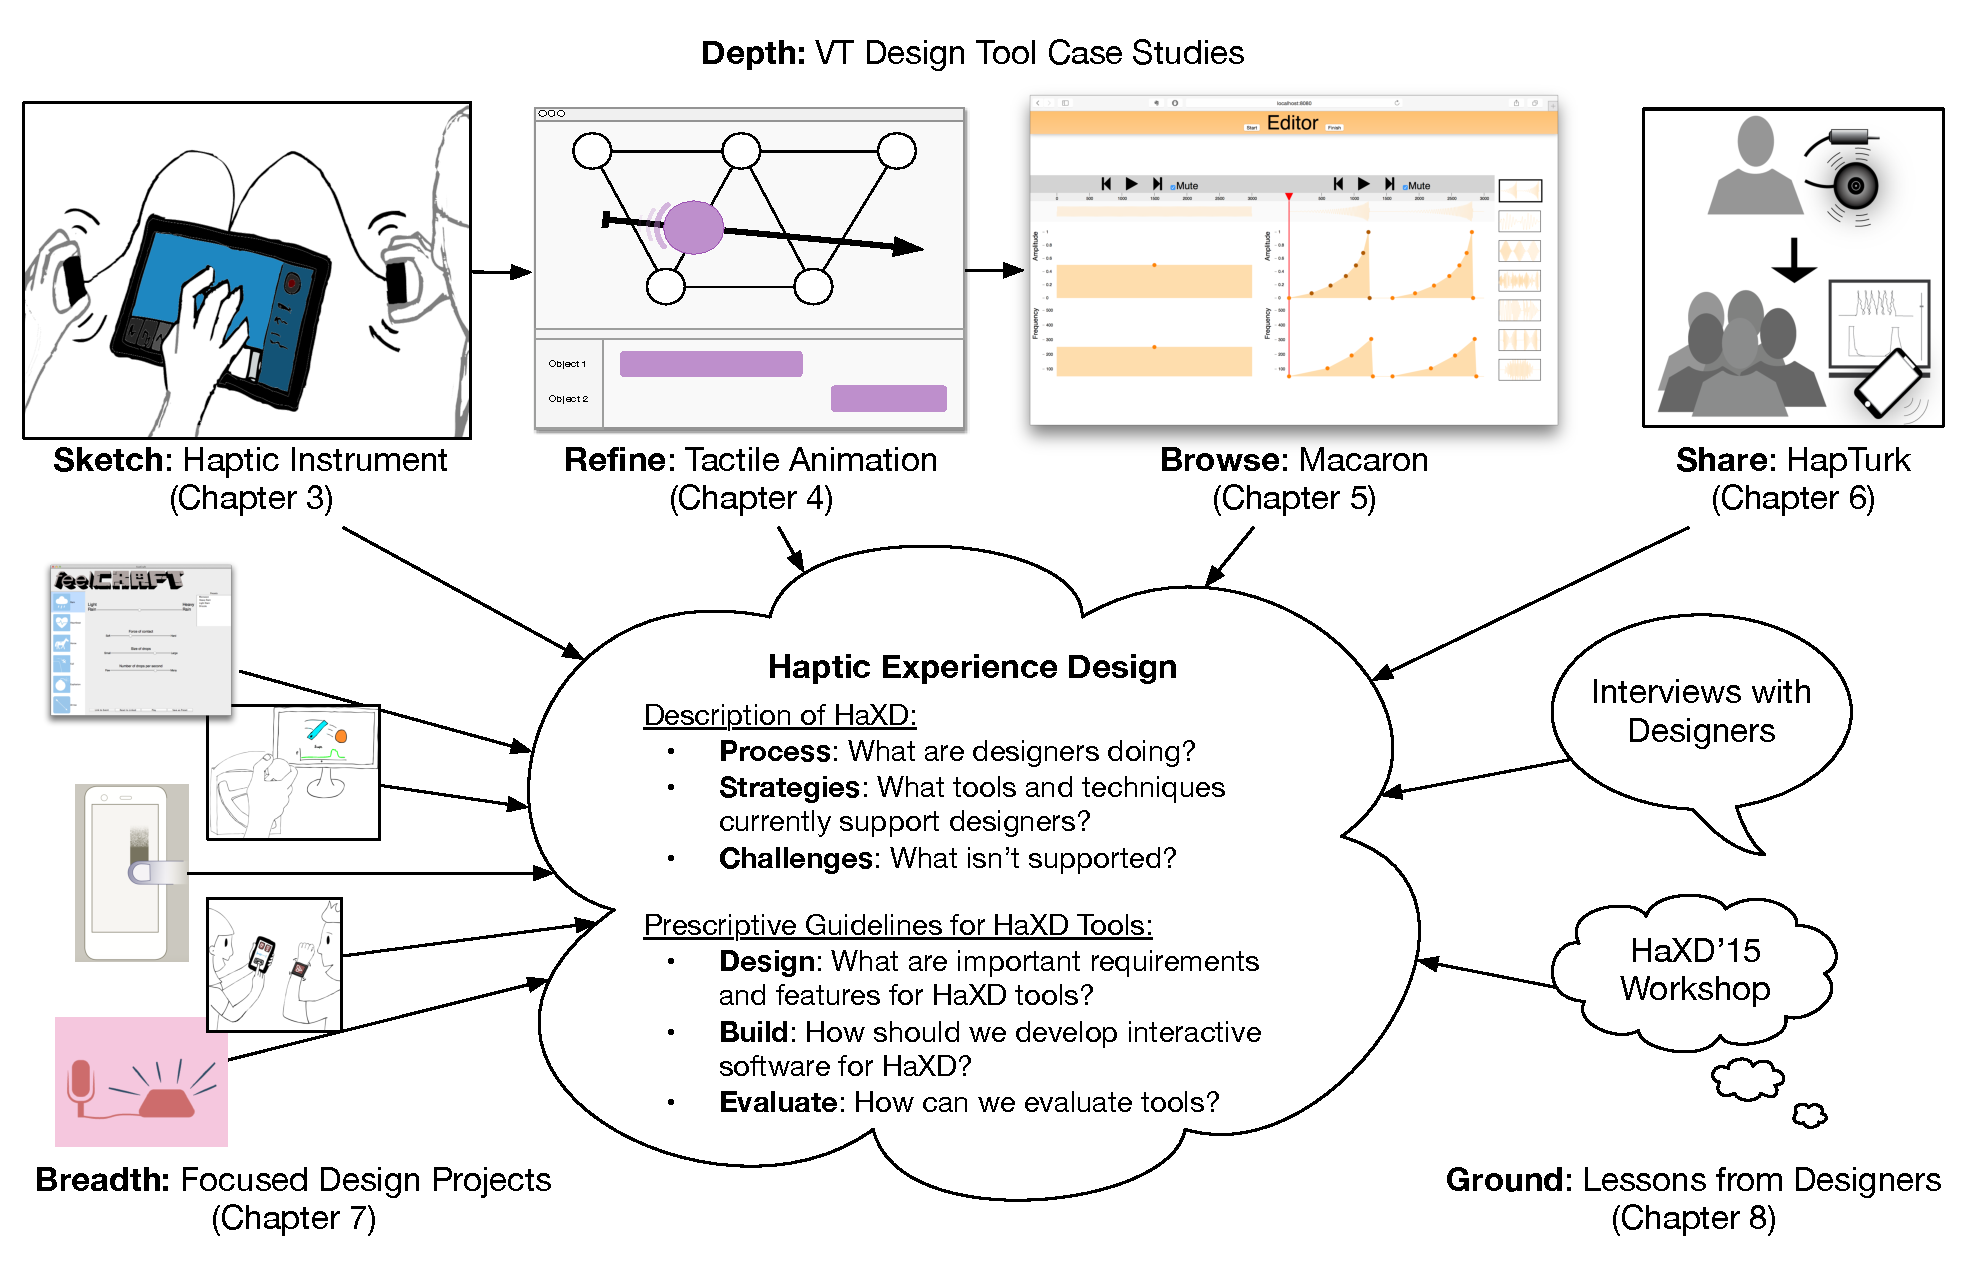
\includegraphics[width=\textwidth]{HaXDTheoryOutline-2016-08-11}
\caption{Approach overview. We investigate VT design tools (Chapters \ref{ch:hapticinstrument}-\ref{ch:macaron}) and techniques (Chapter \ref{ch:hapturk}) in-depth. These findings are synthesized with multiple, smaller focused projects (Chapter \ref{ch:applications}) and grounded data from hapticians (Chapter \ref{ch:hapticianinterviews}) into a preliminary understanding of \haxd.}
\label{fig:intro:methodologyoverview}
\end{center}
\end{figure}



\section{Approach}
While many tools exist to support design in other modalities, such as graphic design, there are few for haptics.
%Part of this comes from immaturity of the field and lack of market penetration of highly expressive haptic devices.
%However, there are also intrinsic challenges to designing for the sense of touch.
%I want to develop practical tools that support the HaXD process, building a body of knowledge of how to facillitate this difficult subfield of design.
We approach this problem with three strategies:
\begin{enumerate}
\item \textbf{Depth: Vibrotactile design tool case studies (Chapters \ref{ch:hapticinstrument}-\ref{ch:hapturk}).}
To understand design, I take a design perspective.
In each of three case studies, I design, build, and evaluate a tool or technique to support an aspect of \haxd, scoped to \emph{vibrotactile} (VT) design.
Each of these results in concrete implications for designing tools and a small window onto the larger HaXD process.
Contributions include algorithms, data structures, interaction techniques, features, analytic techniques, and working software tools that have been employed by designers.
\autoref{ch:hapticinstrument}, \autoref{ch:tactileanimation}, and \autoref{ch:macaron} outline iterative development and evaluation of VT design tools; \autoref{ch:hapturk} covers a VT design technique (proxies).

\item \textbf{Breadth: Focused haptic design projects (Chapter \ref{ch:applications}).}
While the case studies provide an in-depth investigation into VT sensation design, results may not generalize to other devices, and provide limited investigation into application areas like education.
To generalize from VT effects, explore other aspects of haptic design, and gain personal experience as a haptic experience designer, we participate in several smaller focused design projects, which lend a broader context to our findings.
\autoref{ch:applications} discusses these projects.

\item \textbf{Ground: Data from haptic experience designers (Chapter \ref{ch:hapticianinterviews}).}
Finally, despite the recent growth of the field, haptic designers remain relatively rare and difficult to recruit.
To complement our primarily design-based approach and ground it with haptic experience designers in the field, we draw from other data sources: a workshop held at World Haptics 2015 and interviews with haptic designers.
\autoref{ch:hapticianinterviews} discusses this characterization of haptic experience design.
\end{enumerate}


\begin{figure}[htbp]
\begin{center}
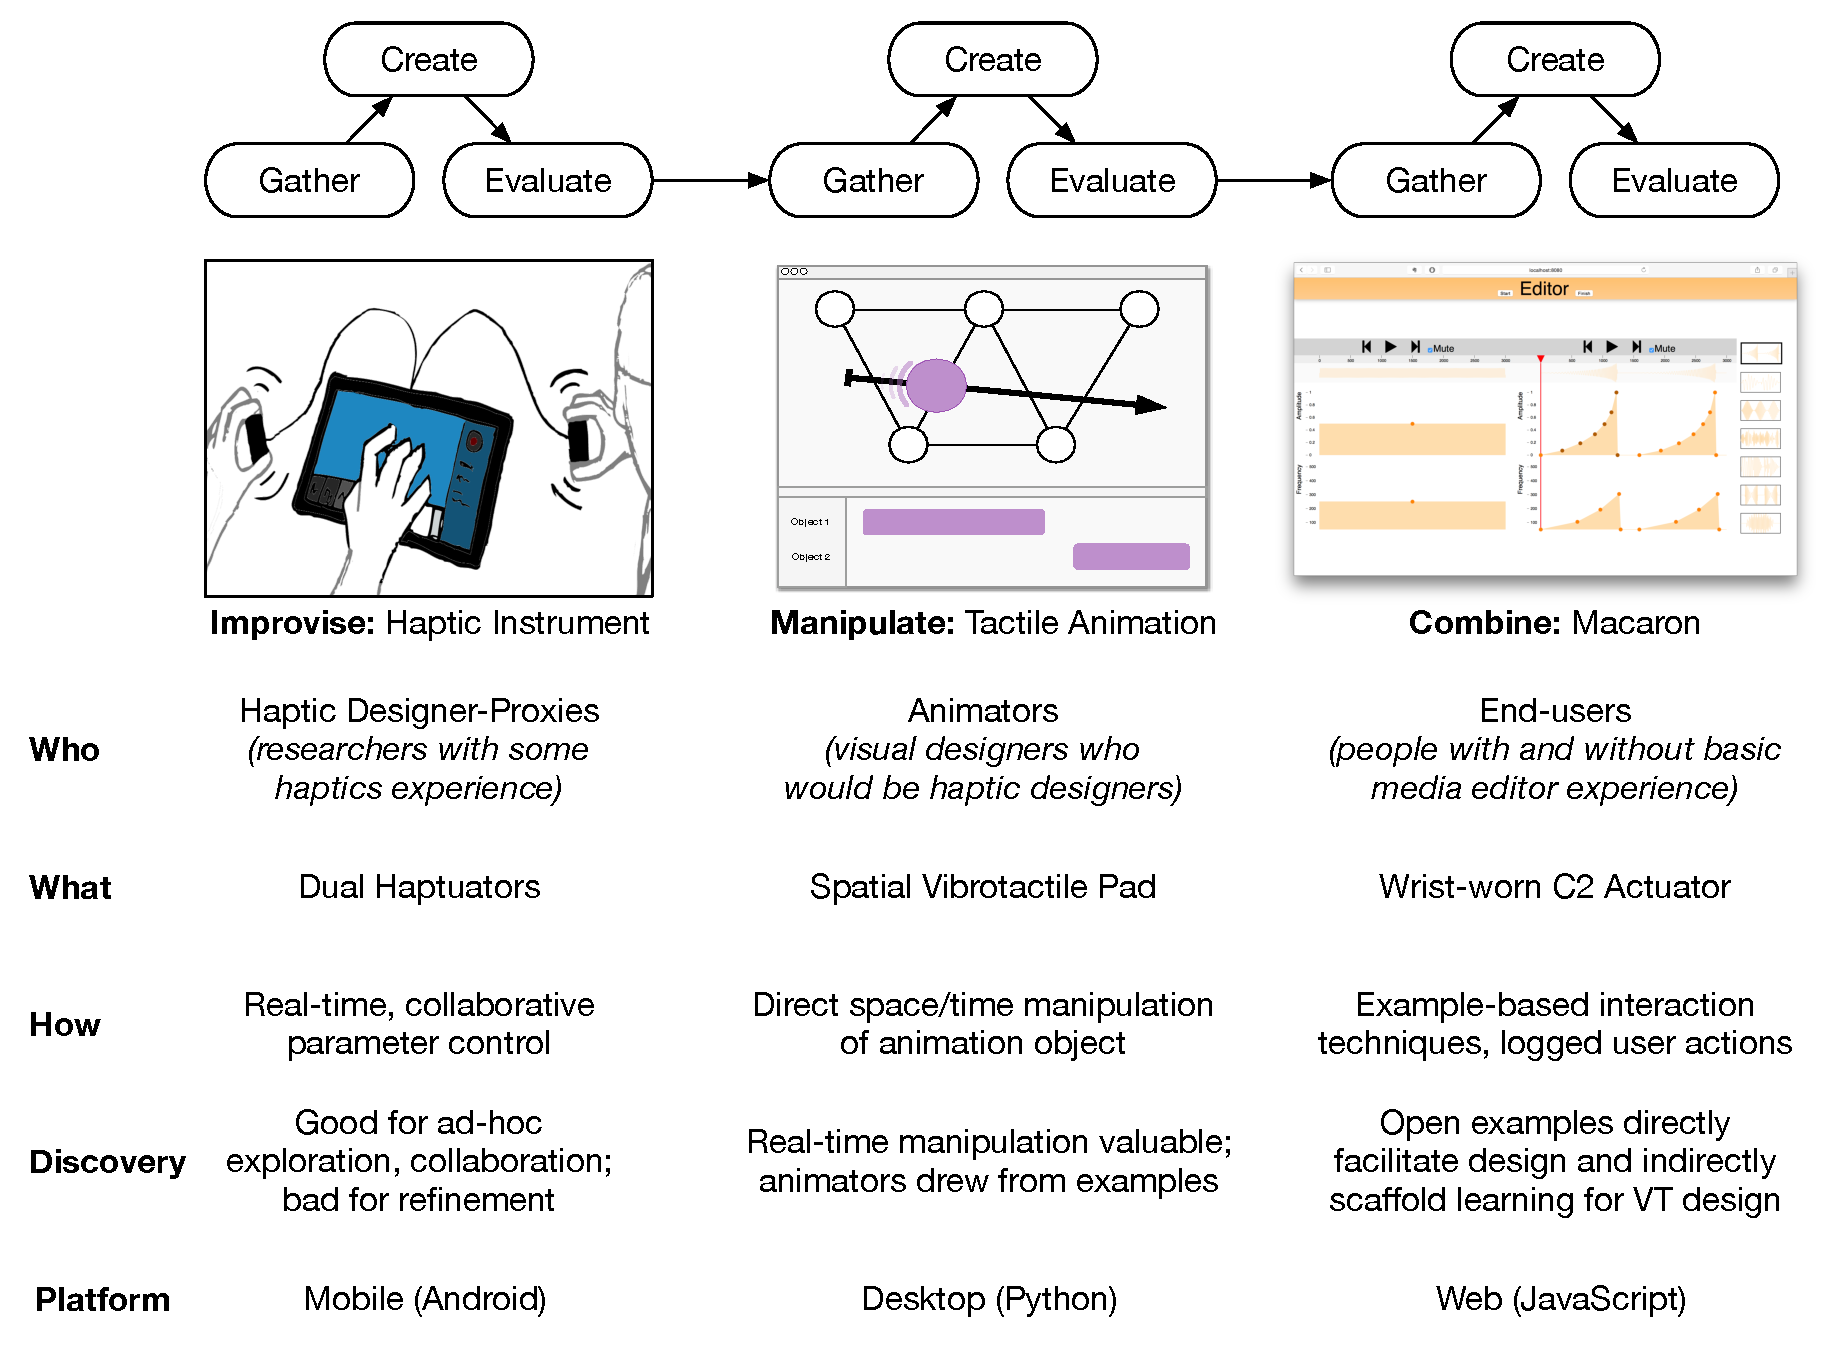
\includegraphics[width=\textwidth]{HaXDTheoryCaseStudyOutline-2016-08-11}
\caption{Vibrotactile design case studies. Each studies an aspect of vibrotactile design with a varied set of users, devices, platforms, and foci.}
\label{fig:intro:casestudyoverview}
\end{center}
\end{figure}



\subsection{Depth: Vibrotactile Design Tool Case Studies}

Each case study investigates a different set of design concepts with varying user populations, VT device, and design challenges.
We iteratively develop three \haxd support tools (\autoref{fig:intro:casestudyoverview}), but restricts scope to VT sensations.
This offers a deep look into an expressive and increasingly common class of haptic devices, allowing us to explore critical features in a somewhat controlled fashion.
An iterative approach allows us to refine ideas and methods, and so each case study follows three steps: \emph{gather}, finding requirements and previous design elements; \emph{create}, where we design and build the tool; and \emph{evaluate}, where we test the tool with its target population and consolidate lessons learned.
We also include a collaborative study for a VT design technique (``HapTurk").


\begin{description}

\item[Initial Exploration: The Haptic Instrument (\autoref{ch:hapticinstrument})]
In Study 1, the Haptic Instrument, we focus on real-time, rapid design of VT sensations with a first look into themes of real-time design and collaboration.
When participants worked with our tool, mHIVE (a ``mobile Haptic Instrument for Vibrotactile Exploration"), compositions couldn't be edited, suggesting mHIVE was suitable for exploration and improvised communication, but not as suited to refining ideas.
We also found informal, collocated collaboration useful, but leave future examination of collaboration support to side projects (described next in \autoref{ch:intro:approach:breadth}).

\item[Direct Manipulation Pipeline: Tactile Animation (\autoref{ch:tactileanimation})]
In Study 2, Tactile Animation, we developed a single abstracted animation object directly manipulated in both space and time.
In this study, we focused on building a usable tool to support exploration and refinement, and investigate a generalized rendering pipeline in detail to understand how to build haptic design tools.
Animators found our tactile animation tool, Mango, easy-to-use, and confirmed our findings about the value of real-time exploration.
We also found that ``soft features", like copy/paste and undo/redo, were extremely important.

\item[Example Use and Analytics: Macaron (\autoref{ch:macaron})]
One stand-out result from both Mango and mHIVE is that designers drew from their experience or examples found in the world, and wanted to re-use what they had created (e.g., through copy and paste).
In Study 3, we explore the role of examples in haptic design with a web-based tool, ``Macaron", a vibrotactile track-based editor with visible, incorporable examples directly embedded in the interface.
Macaron was implemented using the understanding we gained from Study 2, giving us more opportunity to focus on capturing and studying the design process, especially using interaction logs to investigate example use.
%This study is codenamed ``Project Macaron" and consists of two phases.
%Phase I, ``algorithms and interaction techniques", builds a set of perceptually-verified ways to manipulate examples and incorporate them into designs.
%In Phase II, we use the results of Phase I to create a haptic design gallery interface, and study how and when users incorporate examples into their VT designs.
%In this way we hope to consolidate our findings from mHIVE and Mango, and capture our participants' design process more concretely through logging of user actions.
We found examples were used primarily as templates to inform initial design, making each individual design easier but also scaffolding the user's understanding of how to create VT effects.
%These studies are described in more detail in \autoref{ch:hapticinstrument},  \autoref{ch:tactileanimation}, and \autoref{ch:macaron}.

	\item[Feedback at Scale: HapTurk (\autoref{ch:hapturk})]
	%is a collaboration with PhD candidate Hasti Seifi on different techniques to crowdsource feedback on VT icons. Master's student Salma Kashani and undergraduate Matthew Chun are developing visualizations and low-fidelity VT icons during summer 2015.
	While not an iterative design tool study, HapTurk is a focused investigation of a VT design technique for collecting large-scale feedback on VT icons.
	Haptic devices cannot be sent to hundreds or thousands of people for feedback, but collecting in-lab feedback can be expensive, and informal feedback from colleagues is limited in scope.
	We investigate whether visual or low-fidelity \emph{proxies} can stand in for high-fidelity VT effects, with implications for both collecting feedback and broadcasting VT sensations more widely.

\end{description}




\subsection{Breadth: Focused Haptic Design Projects}
\label{ch:intro:approach:breadth}
Each case study provides concrete knowledge for building a VT authoring tool, and some insight into the VT design process.
However, VT technology can be used in many different scenarios, and there are many devices and experiences that involve other haptic modalities.
To broaden our understanding of haptic design, we undertook several more focused haptic design projects to look at different activities, application areas, and haptic modalities.
In \textbf{\autoref{ch:applications}}, we describe several smaller projects that gave opportunities for practicing haptic design and exploring other types of haptic feedback:

\begin{description}
	\item[FeelCraft (\autoref{sec:applications:feelcraft})] is a plug-in architecture that augments media with customizable spatial VT effects.
	We use FeelCraft to explore existing infrastructure for haptic media, and to design VT effects for a popular video game, MineCraft.
	
	\item[Feel Messenger (\autoref{sec:applications:feelmessenger})] is a chat program augmented with expressive, customizable VT effects using commodity hardware and APIs.
	
	\item[RoughSketch (\autoref{sec:applications:roughsketch})] is a painting application for the TPad Phone, a variable-friction mobile device, for the World Haptics 2015 Student Innovation Challenge. 
	Variable friction is a significant contrast to VT sensations as it is intrinsically connected to input: no sensation can be felt without active movement by the user.
	
	\item[HandsOn (\autoref{sec:applications:handson})] is a conceptual model for creative education software using low-cost, DIY haptic hardware, giving us an understanding of how to work with 1-degree of freedom force feedback and an educational context.

	\item[CuddleBit (\autoref{sec:applications:cuddlebit})] is a project inspired by the Haptic Creature \cite{Yohanan2011affectivetouch,Yohanan2011affectdisplay,Chang2010} and CuddleBot project \cite{Allen2015cuddlebot}.
	We use small, breathing robots to explore the display of emotion, and extend our findings from VT design tools into new tools for this modality: Voodle and MacaronBit.

\end{description}





\subsection{Ground: Data from Haptic Experience Designers}
%In addition, it is difficult to find and recruit haptic designers.
\osC{TODO: Update this once I've gone over Ch8 again}
I will synthesize findings from the three design case studies together with a number of side projects, the design literature, community feedback from a workshop on haptic experience design, and interviews with haptic designers into a preliminary design theory on how to support the creation of engaging, captivating haptic experiences.
I expect to make progress on the following questions:


\begin{description}
    \item[Description of the Haptic Design Process.]
    What are the major \textbf{processes and tasks} conducted by haptic designers?
    What \textbf{strategies} do haptic designers employ, including existing tools?
    What are the \textbf{challenges} haptic designers face?
    
    
    \item[Prescriptive Implications for HaXD Tools.]
    What are major \textbf{requirements} and \textbf{features} for designing HaXD tools?
    What are some considerations when \textbf{implementing} HaXD tools in software?
    How can we \textbf{evaluate} design tools effectively?
\end{description}


\section{Outline and Contributions}
\osC{I've already outlined what I'm talking about. What else can I put here to set up the dissertation?}
\osC{TODO: unite this text with some of the previous descriptions, somehow.}
This dissertation continues as follows.
First, in \autoref{ch:rw}, I cover related work with an overview of haptic technology and applications, a presentation of existing haptic design tools, and a discussion of design theory from other fields.

Then, I outline each VT design tool case study in \autoref{ch:hapticinstrument},  \autoref{ch:tactileanimation}, and \autoref{ch:macaron}.
In \autoref{ch:hapticinstrument}, we present findings from our first vibrotactile design tool, the haptic instrument, which supported easy exploration and informal feedback, but identified a key problem: lack of refinement for designs.
In \autoref{ch:tactileanimation}, we present findings from our second vibrotactile design tool, Mango, which established a generalized pipeline and was able to support both exploration and refinement for expert visual animators; it highlighted reuse as an important next step.
In \autoref{ch:macaron}, we present findings from our third vibrotactile design tool, Macaron, which implemented a browsing interface and analytics system; we found examples played a large part of the design process, and that a web-based tool allowed for easy deployment.

%Each chapter is presented as a direct outline of what will appear in the final dissertation, summarizing either methods and results (\autoref{ch:hapticinstrument} and \autoref{ch:hapticanimation}) or proposed methods and possible results (\autoref{ch:hapticexamples}).
I then describe focused haptic design projects in \autoref{ch:hapturk} and \autoref{ch:applications}, and the results from our grounded data collection in \autoref{ch:hapticianinterviews}.\
In \autoref{ch:hapturk}, we document findings from HapTurk, a technique for getting feedback on vibrotactile designs at scale: from the crowd using proxy vibrations distributed over Mechanical Turk; we also comment on uses for haptic broadcasting.
In \autoref{ch:applications}, we synthesize together findings from our side projects, showing generality by applying our understanding of haptic design explicitly in several domains and gaining practical experience designing haptic experience.
In \autoref{ch:hapticianinterviews}, we complement our design-based inquiry through interviews with professional haptic designers and a workshop run to elicit feedback from the community; this captures a description of haptic design, reinforcing our findings for important support tools, and identifies more systematic challenges.

Finally, in \autoref{ch:conclusion}, we conclude with a summary of our final results and directions for future research.


%
% END
%
\endinput

Any text after an \endinput is ignored.
You could put scraps here or things in progress.


%    2. Main body
% Generally recommended to put each chapter into a separate file

%% The following is a directive for TeXShop to indicate the main file
%%!TEX root = diss.tex

\chapter{Background}
\label{ch:rw}

In this chapter, we provide the relevant background for this dissertation.
We begin with an overview of haptic technology and perception.
Next, we discuss the application space for haptics and why haptic experiences are increasingly important to design.
We then discuss the previous work in \haxd and related support tools, identifying why this is an area for improved understanding.
After, we discuss non-haptic creativity support tools and design theory which provided inspiration and guiding principles.
Finally, we present the qualitative and quantitative methodologies used in this dissertation.
Throughout the chapter, we contextualize this work and \haxd in both the haptics and HCI communities.


%%%%%%%%%%%%
%
% SECTION: What is haptics?
%
%%%%%%%%%%%%
\section{An Overview of Haptic Technology and Perception}
The term ``haptic" was coined by German researcher Max Dessoir to refer to the study of touch, in a similar to ``optic" for sight and ``acoustic" for sound \cite{Grunwald2008}.
Today, it refers to both the study of the psychology and perception of the senses of touch, and the technology that employs touch as a method of feedback.
Haptic technology is typically separated into two classes based on the main sense modality: \emph{tactile} sensations, and \emph{proprioception}, or the sense of body location and force;  the latter includes \emph{kinaesthetic} senses of force and motion.
These two types of feedback are useful for different purposes, \eg, people use their fingerpad's tactile senses to derive texture, but kinaesthetic feedback to infer weight \cite{Lederman1987};
different senses can be combined for more convincing results \cite{Okamura1998}.
An excellent overview of the haptic senses is available by \citet{Lederman2009survey}, and a practical introduction to the technology is available by \citet{Hayward2007}.
Here, we focus our coverage on the sensations directly studied by this dissertation, while also portraying the diversity of haptic experiences and technology.

\subsection{Tactile Perception and Technology}
%\osC{Goal: Explain the main mechanisms we use in the dissertation's studies, persuade the reader that I know enough about tactile perception, and show the variety of tactile displays and experiences.}
Tactile sensations rely on multiple sensory organs in the skin, each of which detect different properties, \eg, Merkel disks detect pressure or fine details, Meissner corpuscles detect fast, light sensations (flutter), Ruffini endings detect stretch, and Pacinian corpuscles detect vibration \cite{ChoiKuchenbecker2013}.
%Temperature and pain are also detected through \osC{todo}.
Of these, the Pacinian corpuscle is most widely targeted by technology through vibrotactile (VT) sensations, where vibrations stimulate the skin.
VT sensations are accessible, well-studied, and increasingly widespread, and can be passively felt, easing implementation.
Our in-depth design tool studies thus focus on VT experiences.

VT actuators can take may forms.
Eccentric mass motors (sometimes ``rumble motors" or ``pager motors") are found in many mobile devices and game controllers, and are affordable but inexpressive.
%An unbalanced mass is mounted on the motor, which provides dramatic shaking of the device.
More expressive mechanisms such as voice coils %  implemented in a variety of ways and 
offer independent control of two degrees of freedom, frequency and amplitude.
Piezo actuation is a very responsive technique that is typically more expensive than other vibrotactile technology.
% One of the more common and expressive is the C2 tactor, intended to directly stimulate the skin through contact or a thin membrane; the tactile animation project [] uses an array of C2 tactors.
While voice coils typically directly stimulate the skin, linear resonant actuators (LRAs) shake a mass back and forth to vibrate a handset in an expressive way; a common research example is the Haptuator \cite{Yao2010}.
Instead of directly stimulating the skin, this actuator typically shakes another device held by the user, such as a mobile device \cite{Yoo2014} or pen \cite{Culbertson2014}.
As of writing (2016), this type of actuator is increasingly deployed in consumer products (\eg, Apple's Taptic Engine).

%%%%In contrast to displacing the entire user body, recent multichannel haptic devices create percepts of dynamic and localized haptic sensations directly on the user's skin \cite{Israr2011} and in the mid-air \cite{Wilson2014}.
Actuators like VT devices can be used alone or put together spatial multiactuator displays like seats \cite{Israr2012,Israr2010}, belts \cite{Pielot2009,Paneels2013}, wristbands \cite{Arab2015,Paneels2013,Gupta2016}, vests \cite{Prasad2014,Jones2004}, and gloves \cite{Park2016,Kim2009}.
These can be arrange into grids, either dense tactile pixels (``taxels") \cite{Kim2009} or sparse arrays \cite{Israr2012,Israr2010}, to provide explicit 2D output on a plane.
Multiactuator arrays increasingly exploit tactile illusions to create effects of motion or phantom sensations in-between actuators.

Another emerging tactile feedback mechanism is programmable friction.
Surface friction, for example on a mobile touch screen, can be manipulated by both mechanical motion or electrical adhesion.
The TPad \cite{Winfield2007a} vibrates a plate at ultrasonic frequencies to create a cushion of air between the surface and the user's finger.
This effect is programmable, and can be used to with a number of interactive scenarios \cite{Levesque2011}.
Other techniques like electrovibration, deployed in TeslaTouch \cite{Bau2010}, and electrostatic forces \cite{Meyer2013} can create a similar effect.
Strong electroadhesion \cite{Shultz2015} has the potential to create even larger shear forces, but comes with a high power cost.
In RoughSketch (\autoref{ch:applications}), we design for a mobile version of the TPad deployed on Android devices, the TPad phone (\url{www.thetpadphone.com}).

There are many other types of tactile stimulation used in haptic experiences.
2-dimensional pin-based grids like Optacon \cite{Bliss1970} and HyperBraille (\url{www.hyperbraille.de}) can display Braille and 2D images to the blind and visually impaired, and operate as a generic computer display \cite{Prescher2010}. 
%"Survey on communication through touch" by pasquero, "Optical to tqactile image conversion for the blind by Bliss et all 1970.
Similar multi-point displays have been deployed on mobile devices.
Edge Haptics uses dozens of linearly-actuated pins on the edge of a mobile device for tactile stimulation, similar to a 2-dimensional braille pin display \cite{Jang2016}, while laterally moving pins can use skin-stretch as a display mechanism \cite{Luk2006}.
Electrocutaneous stimulation, where electrodes are directly activated on the skin, has been deployed for spatial tongue displays \cite{Bach-y-Rita1998}.
Temperature displays exploit warm and cold receptors in thea skin for display, using Peltier junctions \cite{Jones2002}.
Tactile sensations can be created at a distance using ultrasonic transducers \cite{Obrist2013,Carter2013} and vortex cannons that shoot puffs of air \cite{Sodhi2013}.



\subsection{Proprioception and Force Feedback}
%\osC{Goal: Explain the main mechanisms we use in the dissertation's studies, persuade the reader that I know enough about proprioception, and show the variety of force-feedback displays. This section will be smaller than the tactile section, and should make the distinction of verisimilitude and veridicality a bit clearer, because with FF we often have a virtual environment and are more concerned with passivity, stiffness, etc.}
Proprioception, the sense of force and position, is synthesized from multiple sensors as well: the muscle spindle (embedded in muscles), golgi-tendon organ (GTO) in tendons, and tactile and visual cues \cite{Kandel2000}.
We distinguish proprioception from the related term kinaesthetic by being the general, synthesized sense, where kinaesthetic sensation is strictly the sense of motion \osC{todo: make sure this is correct}.
Force displays are common in precise, specialized applications like robot-assisted surgery \cite{Okamura2009} or realistic sensorimotor training environments \cite{VanDerMeijden2009}.

Force-feedback devices might have degrees of freedom of feedback (DoF), the number of forces or torques they can display.
These devices render a \emph{virtual environment}, with simulated forces depending on the input from the user.
Common consumer-facing 3-DoF devices include the Geomagic Touch (previously the Sensable PHANTOM) and Falcon devices, offering force in three directions.
2-DoF designs like the pantograph \cite{Ramstein1994,Campion2005} can provide displays on screens, walls, and tables.
These displays have previously input on realistic simulation and rendering: \eg, making free space feel free, providing stiff virtual objects and walls, and avoiding saturation  \cite{massie1994phantom}.
Open-hardware, self-assembled versions of these devices, such as WoodenHaptics \cite{Forsslund2015} for 3-DoF devices and Haplet \cite{Gallacher2016} for 2-DoF displays, have the potential to make haptics more accessible.
Much previous work has been done on handling technical concerns, \eg, displaying complex polygonal objects with a ``God object" \cite{Zilles1995}, coordinating remotely situated devices or shared environments \cite{Buttolo1997}, and improving collision realism with transient forces \cite{Kuchenbecker2006}.
More complex environments are primarily programmed in using APIs like CHAI3D, OpenHaptics, or Unity.

Another approach is to use simple force feedback, especially for haptics education \cite{Jones2014}.
1-DoF devices include linear actuators pushing on the user and haptic knobs, \eg, the UBC Twiddler \cite{Shaver2003,Enriquez2003,MacLean2009a}, and paddles, \eg, the HapKit \cite{Martinez2016}.
The UBC SPIN lab has also adopted 1-DoF force feedback in its affective robot, the Haptic Creature \cite{Yohanan2011affectdisplay,Yohanan2011affectivetouch}, the CuddleBot, and CuddleBits \cite{cang2015cuddlebits}.
We explore force-feedback design with the HapKit and CuddleBits in \autoref{ch:applications}.


\subsection{Haptic Illusions}
Like visual displays' stroboscopic effect transforming a series of images into the perception of motion, illusions play a valuable role in haptic sensations \cite{Hayward2016}.
Some effects are influenced by other senses.
In the classic size-weight illusion \cite{charpentier1891analyse}, when two weights have the same mass but different sizes, the smaller is perceived to be heavier, whether size is seen or felt \cite{Hayward2016}.
A striking, recent example is the use of visual dominance to use a single physical block to provide haptic feedback for multiple virtual blocks by distorting the visual position of the user's arm \cite{Azmandian2016}.
We employ similar techniques in our FeelCraft and Feel Messenger projects, using visual feedback to prime users to haptic sensations (\autoref{ch:applications}).

Other illusions are purely tactile and useful for grid displays.
Phantom tactile sensations \cite{Alles1970}, create illusory vibrations in between two or more VT actuators, opening up the space in-between actuators for display.
Continuous motion can be simulated, \eg, \citet{Seo2010} created a perceived motion flow between two VT actuators mounted on the ends of a handheld device by controlling their intensity.
Similarly, \citet{Lee2012a} created across-the-body and out-of-the-body illusions on a mobile device using up to four % inexpensive 
linear resonant actuators; \citet{Gupta2016} used interpolation on a VT wristband for new interaction techniques.
The Tactile Brush algorithm \cite{Israr2011a} combined phantom tactile sensations and apparent tactile motion to render high-resolution and moving haptic patterns on the back using a coarse grid of VT actuators. 
Other spatio-temporal VT illusions such as the ``cutaneous rabbit"  \cite{Tan2009}, where carefully timed discrete tactile stimuli create perceived motion, and Tau and Kappa effects \cite{Hayward2008,Hayward2016}, where perceived distance between stimuli depending on their timing, can also be used with VT arrays.
Similar illusions are possible using other tactile modalities, including temperature displays \cite{Singhal2016} and electrocutaneous stimulation \cite{Tanie1980}.
We extend phantom sensations to 2D interpolation (\eg, between 3 actuators) to enable Tactile Animation (\autoref{ch:tactileanimation}).



\osC{Integrate this}
Of course, haptic perception can depend on the situation of the user, especially important in wearable contexts.
Vibrotactile detection depends on many variables, including location on the user's body, how much the user is moving, and whether they are expecting the vibration \cite{Karuei2011}, and social context \cite{Cauchard2016}.
These effects can be mitigated through sensing, \eg, detecting movement with accelerometers \cite{Blum2015}.




%\inlineHeading{Multimodal interaction}
%Similar to vision and audio, haptic perception is susceptible to illusions \cite{Hayward2016,Hayward2008}.
%
%discuss passiveness, like cobots, etc.

%%%%%%%%%%%%
%
% SECTION: Why should we care about haptics?
%
%%%%%%%%%%%%
\section{The Value of Haptic Experiences}
Haptic feedback can provide several benefits to interactive experiences.
Here, we outline the main benefits haptics provides, and then several application areas that commonly leverage those benefits.


\subsection{Why Touch?}
Haptic technology enables information transfer between humans and computers;
this transfer is rich, proximal, and fast.
Information flows both ways, through input and output, sometimes simultaneously.
We focus on designed haptic display.

One advantage of touch is simply that it is not vision or audio, the primary feedback methods for interactive systems.
Haptic technology can reinforce other modalities, enriching feedback for a more complete experience, or
provide complementary feedback, with many possible reasons:
information saturation, \eg, when visual or audio displays have maximized their output;
task context, \eg, when the user is driving and must keep their eyes on the road;
impairment or impairing situations, \eg, when a user has limited sight or hearing;
ambient displays, \eg, keeping a user aware of a piece of information without interrupting them;
or nature of the information, \eg, communicating emotion.
%It can increase general usability and provide an alternative path for information when other modalities are not available (\eg, the users are visually-impaired) or not appropriate (\eg, looking at a screen would be socially inappropriate).
Sensory substitution, first pioneered by Bach-y-Rita \cite{Bach-y-Rita1969}, is a dramatic technique often using haptic senses to augment or replace other senses.
A wide variety of devices have been developed and studied for the visually impaired (\eg, \cite{Prescher2010,Bliss1970}).

Of course, touch is a unique, rich sense in its own right.
Like sound, touch can be invisible; like vision, it can be spatial.
Feeling an object is especially helpful at discerning material properties \cite{Lederman1987}.
Touch is the first sense to develop, playing an important role in formative experiences \cite{Jansson-Boyd2011}.
Sensorimotor actions can help to scaffold understanding through embodied learning \cite{Papert1980}.
Touch can also be used for artistic expression; \citet{Gunther2002} studied a full-body vibrotactile suit to create music-like ``cutaneous grooves", helping to identify the artistic space of VT sensations, including concerts with tactile compositions.

While haptic feedback can improve usability and task performance \cite{Pielot2009,Chan2008}, touch is especially connected to visceral, emotional connections.
Marketing research has studied multiple ways that touch can connect with customers.
For example, the way a smartphone feels can influence a purchase over one that might work better, and customers prefer to shop at stores that let them touch products \cite{Spence2011,Jansson-Boyd2011}.

There are different models of models used in affective computing.
Two especially common models are Ekman's basic emotions and Russell's affect grid.
Ekman's basic emotions \cite{Ekman1992,Ekman1971} are a discrete set of emotions identified from a cross-cultural study of facial expressions; we use this model's emotions as the design task in \autoref{ch:hapticinstrument}.
Russell's affect grid \cite{Russell1989circumplexmodel,Russell1989affectgrid} separates emotions into dimensions of arousal (low to high energy) and valence (positive and negative emotions); this work informs much of our work on expressivity and especially the CuddleBit work in \autoref{sec:applications:cuddlebit}.

Researchers are starting to develop design guidelines to express emotions through haptic experiences.
Low-level parameters like amplitude, frequency, and duration have been linked to emotions: \citet{YongjaeYoo2015} showed that VT icons can express arousal and valence;
\citet{Obrist2015} established design parameters for mid-air ultrasound stimulation.
Because touch can be bidirectional, affective sensing can accompany haptic display.
Through the Haptic Creature project established a touch dictionary of gestures used to emotionally communicate with robots \cite{Yohanan2011affectivetouch}.
Touch-based surfaces can detect these gestures \cite{Flagg2013} through technologies like conductive fur and fabric \cite{Flagg2012}.






%emotion theory background
%Emotion can play different roles in technology, such as affective technology, hedonic qualities, or interactional dynamics \cite{Hook2008bodyemotion} \osC{need to dig deep to understand this}





%; see \citep{Hamilton-Fletcher2016} for a recent survey and discussion of user preferences.


%In many of these contexts, careful design is required.
% \citet{Arab2015}'s wrist based display worked best when using a metaphor-based approach \cite{Brunet2013a}, co-designing metaphors with their users.
% \citet{Cauchard2016} found rhythm-based pulses were more effective for portraying numbers in their in-situ study.




\subsection{Applications}
While realistic virtual environments for force-feedback haptic feedback is extremely helpful in medical or training applications \osC{todo}, we focus on applications that find increased value in an explicit design step.


\subsubsection{Immersive Media and Virtual/Augmented Reality}
A popular application for haptic experiences is augmented, immersive media experiences.
Actuated tactile feedback has been used as early as 1959 in the movie \emph{The Tingler}  \cite{IJsselsteijn2003}.
4D theatres and theme park rides use bursts of air or water sprays to engage the audience.
Companies like D-Box (\url{www.d-box.com}) augment films with haptic tracks that both low-frequency movements and high-frequency vibrations, and can be found in theatres across the world.
Buttkicker (\url{www.thebuttkicker.com}) also augments 4D theatres, and provides products for home theatre setups.

Haptic experiences are also increasingly of interest in virtual reality (VR) environments.
Skin stretch techniques, explored in \cite{Guinan2014} and now commercialized by Tactical Haptics (\url{tacticalhaptics.com}), augments virtual-reality setups by simulating forces and torques using handheld controllers, lending stronger immersion for virtual environments and VR games.
Haptic Turk \cite{Cheng2014} and TurkDeck \cite{Cheng2015} are innovative explorations of high-fidelity haptic experiences in virtual environments using people as actuators.
Impacto uses electrical muscle stimulation and a solenoid actuator to create wearable haptic feedback with both kinaesthetic and tactile feedback \cite{Lopes2015}.
Haptic retargeting distorts visual feedback to re-use a single physical block in a virtual block-building game \cite{Azmandian2016}.


Previous work has also attempted to add greater immersion to broadcast media by including haptic sensations.
\citet{Modhrain2001} present an early vision of Touch TV, using active touch with two-DOF actuators embedded in remote controllers; \citet{Gaw2006} follow up with editable position playback on a force-feedback device, played alongside movies or cartoons.
More recently, the proliferation of online streaming video has developed opportunities to add haptic sensations using novel data structures.
Tactile Movies \cite{Kim2009} looks into augmenting movies with spatial VT feedback, including an authoring interface.
\osC{todo} YouTube  \citet{Gao2013}
haptic-audiovisual (HAV) content \cite{Danieau2013} basics of composition \cite{Guillotel2016}


\subsubsection{Affective Computing}
We've discussed how touch is closely connected to emotion.
This has implications for design;
%emotional connection and relationship can influence preferred interaction models;
for example, couples are more comfortable with a ``hand stroke" metaphor for two remotely coupled haptic devices than strangers, who prefer a more less intimate ``ping-pong" metaphor \cite{Smith2007}.
Emotional display through touch has therapeutic applications.
\citet{Bonanni2006} created TapTap, a wearable that can record and playback VT equivalents of affectionate touch to support users in therapy.
Tactile displays target improved mental health \cite{Vaucelle2009} and aiding emotional understanding for autism \cite{Changeon2012}.
The Haptic Creature project explores affective touch in human-robot interaction (HRI) \cite{Yohanan2005,Yohanan2009,Yohanan2011affectivetouch,Yohanan2011affectdisplay};
this furry, zoomorphic robot can measurably relax users when they feel it breath \cite{Sefidgar2016}.





\subsubsection{Expressive Communication}
%interpersonal touch, and haptic interpretations of it
Touch is extremely important for interpersonal communication, from greeting a new acquaintance with firm handshake, to showing affection to a loved one; see \citet{Gallace2010} for an overview.
Of course, technologically can mediate touch between people, \eg, in remote collaboration or shared virtual environments \cite{Haans2006}.
\citet{Brave1997} introduced ``inTouch", mechanically linked rollers that enabled playful touch interactions at a distance.
ComTouch \cite{Chang2002a} used pressure input to send vibrations with between mobile phones, finding it was used for attention, turn-taking, and emphasis.
\citet{Hoggan2012} elaborated these findings a one month-study found users sent ``Pressages" (pressure messages) both for greetings and to emphasize speech or emotional messages.
\citet{Chan2008} used VT icons to coordinate turn-taking in an online system, featuring an extensive design process to create and perceptually verify icons that present system state and requests with varying urgency.
%\citet{Brown2006multidimensionaltactons} used tactons displayed on a user's forearm \osC{this is actually kinda boring this study}





\subsubsection{Mobile Alerts}
Mobile contexts are rife with opportunities for haptic feedback.
Ambient tactile displays can provide awareness can provide awareness and alerts without distracting the user.
VT feedback is affordable, low-power, and can be added to watches and wrist-bands \cite{Brunet2013a,Arab2015}, belts, vests, and other wearables.
Tactons \cite{Brown2006} are a type of haptic icon \cite{MacLean2003} that provide VT feedback, commonly in mobile applications.
Rhythm opens up a large design space, letting users learn 84 different icons \cite{Ternes2008} and can be applied with even light, low-cost rumble motors.
A 28-day study showed that rhythmic VT icons do not disturb users in daily activities and can communicate ambient information \cite{Cauchard2016}.
\citet{Hemmert2008} explored a life-like metaphor of pulsing and breathing to provide alerts, but found care needed to be taken to not be annoying.
Multiple actuators can be combined in mobile handheld devices to provide differentiable spatial information, enriching the VT icon design space \cite{Yatani2009a}.
VT icons produced by phones can represent multiple levels of urgency and source of an alert (\eg, voice call, text message, or multimedia message) \cite{Brown2006mobilealerts}.


\subsubsection{Guidance}
Guidance is a typical application for VT feedback, which can be invisible, mobile, and accessed without using vision or sound.
%Guidance is a major applications, especially for specific populations like the visually impaired \cite{} or older adults \cite{Arab2015}.
Spatial guidance through haptic wearable display can improve navigation with multiple actuators across several form factors, including belts \cite{Pielot2009,Lindeman2005}, wrist-bands \cite{Arab2015}, and vests \cite{Prasad2014}; in each case, the vibrations inform the user where to go with spatial vibrations or metaphorical spatial icons.
Periodic vibrations can guide a user's walking speed without large attentional demands \cite{Karuei2014}.
Tactile illusions like saltation can provide directional information for guidance \cite{Tan1997}; larger back-based displays are effective for guiding both attention and direction, \eg, in automobiles \cite{Tan2003}.
\citet{Brewster2010} used VT icons to provide awareness of nearby friends and colleagues.
%Guidance Linderman2005 \cite{Prasad2014} \cite{Pielot2009}





\subsubsection{Education}
Haptic technology has the potential to improve educational resources, especially to those lacking resources.
Montessori methods have long espoused the value of physical learning aids, especially using physical \emph{manipulatives} \cite{Montessori1917}.
There is evidence to support these techniques: in a meta-analysis of 55 studies, \citet{Carbonneau2013} found that physical manipulations improve several learning outcomes, with influence by other instructional variables.
Studies of gestures have also found value in students ``being the graph" by physically acting out mathematical shapes, grounding abstract knowledge in embodied experience \cite{Gerofsky2010}.
These techniques have roots in constructivist learning, where learners use existing understandings as a \emph{transitionary object} to understand new concepts \cite{Papert1980}.

Haptic technology is well-positioned to support embodied learning, and there is early evidence for its efficacy.
Haptic feedback has been shown to improve temporal aspects when training motor skills \cite{Feygin2002}.
In a study for molecular chemistry education, \citet{Sato2008} found students had higher test scores when they interacted with their haptic learning interface; students reported engagement.
In \autoref{ch:applications} we describe results from an early learning interface for low-cost haptic displays \cite{Martinez2016}, showing that haptic technology can improve engagement and make lasting impressions.

%\cite{Hook2008bodyemotion} (?)

%Active learning and creativity in education??

%%%%LEARNING
%%%\osC{Education}
%%%Recognition of the value of a hands-on, embodied approach to learning dates to 1907, when
%%%Maria Montessori opened a school where she used \emph{manipulatives} to teach a wide array of concepts ranging from mathematics to reading, e.g., by introducing the alphabet through children tracing their finger along large, cut-out letters~\cite{montessori_advanced_1917}.
%%%Constructivist learning theories posit that well-designed manipulatives can assist understanding by grounding abstract concepts in concrete representations ~\cite{papert1980,piaget_science_1970},
%%%%Their use today is 
%%%and are an accepted core principle in early math and science education, confirmed empirically~\cite{carbonneau_meta-analysis_2013}. 
%%%
%%%More recently, digital technologies are radically altering learning environments.
%%%Massive Open Online Courses (MOOCs) expand access, games motivate, and with graphical simulations (e.g., PhET~\cite{wieman_phet:_2008}), students can interact with abstractions to develop their understanding.
%%%However, these experiences are disembodied. Indirect contact via keyboard, mouse and screen introduces a barrier of abstraction that undermines the connection and path to understanding. 
%%%% that the interaction aims to promote. 
%%%
%%%
%%%Haptic (touch-based) technology should bring %able to bring
%%% benefits of physicality and embodied learning~\cite{dourish_where_2004} to interactive virtual environments. 
%%%It adds a sensory channel as another route to understanding~\cite{calvert_crossmodal_1998}; when deployed appropriately, active exploration can improve understanding~\cite{martin_physically_2005} and memory~\cite{glenberg_activity_2004} of new concepts. 
%%%Haptic tools have already shown promising results in many specializations, demographics and age groups, both
%%%to enhance lesson fidelity 
%%%% (e.g., physics and medical simulations)  -- don't have room for citations!
%%%and to increase engagement and motivation through tangibility and interactivity; e.g., with devices like Geomagic Touch\footnote{Prev. Sensable Phantom \url{www.geomagic.com/en/products/phantom-omni/overview}}~\cite{williams_implementation_2004} and SPIDAR-G~\cite{sato_haptic_2008}.
%%%
%%%Unfortunately, %t
%%%%These 
%%%%Sadly, 
%%%existing approaches have %suffer from 
%%%both hardware and software limitations.
%%%Actuated learning tools introduce physical issues of cost, storage, and breakage;
%%%devices are  too bulky, complex, or expensive for schools or self-learners.
%%%For software, it is hard for users to construct and explore their own haptic environments. Typically, users load a virtual system to interact with it haptically. This sidelines the rich learning potential of involving users with model construction~\cite{papert1980}.
%%%We address hardware with the HapKit~\cite{martinez_2016}, a \$50, simple, low-fidelity device constructed from 3d printed materials.  
%%%
%%%Our focus here is on software, with a new learning environment that lets users both construct and explore haptic systems. Until now, the only way for a user to construct a haptic system was by programming it herself. Our approach, inspired by Logo ~\cite{papert1980} and Scratch ~\cite{maloney2010}, is to ultimately % KM notes: currently we don't provide much power compared to programming. But it's planned for.
%%%provide much of the power of a programming language while hiding distracting complexity. 
%%%



%%%%%%%%%%%%
%
% SECTION: Why should we care about haptic experience design tools? What is the precise problem this dissertation is solving?
%
%%%%%%%%%%%%
\section{Previous Efforts for Haptic Experience Design}


\osC{just moved this from applications}
The Haptic Application Meta Language (HAML) \cite{Eid2006} is an XML-based data format for adding haptics to MPEG-7 video, eventually augmented with the HAML Authoring Tool (HAMLAT) \cite{,Ferre2008}.
\citet{AbdurRahman2010} eventually adapted an XML approach to YouTube, and \citet{Gao2013} developed related online MPEG-V haptic editing.
Augmented media experiences and HAV content \cite{Danieau2013},  have used different methods of input.
One approach is to use camera motion sourced from accelerometers \cite{Danieau2012} to actuate audience members' hands and head in a HapSeat \cite{Danieau2013a,Danieau2012a}.
Later editable with H-Studio \cite{Danieau2013c}, this work has proposed the concept of Haptic Cinemotography \cite{Danieau2014}, including basic principles of composition when combined with video \cite{Guillotel2016}.
Other approaches include automatic conversion of audio content
Several studies have looked into automatic conversion from audio streams \cite{Lee2013,Chang2005,Hwang2014} or video streams \cite{Kim2014} to VT or force-feedback output.


\subsection{Editors and design tools}
As long as designers have considered haptic effects for entertainment media, they have needed compositional tools % to facilitate their design 
\cite{Gunther2002}.

Custom editors (such as D-Box Motion Code Editor) and software plugins are provided to media designers that overlaid the visual and audio content with haptics, and allow designers to generate, tune and save frame-by-frame haptic content in an allocated track for it to play simultaneously with the media content. 

By tuning parameters of these effects, users could personalize  haptic content, embed it in games and share effects with other users.
Similar devices and authoring schemes are also developed for online social interactions using custom multi-actuator haptic devices \cite{Kim2009,Tsetserukou2009,Paneels2013}.%Tsetserukou, D. and Neviarouskaya, A. iFeel_IM!: augmenting emotions during online communication. Comp. Graphics & Applications 30 (2009), IEEE, 72-80.
A great deal of previous work has focused on how to prototype or author haptic phenomena using non-programming methods. 

Many user-friendly interfaces help designers create % control 
haptic sensations, especially with vibrotactile devices.
The Hapticon editor \cite{Enriquez2003}, Haptic Icon Prototyper \cite{Swindells2006}, and posVibEditor \cite{Ryu2008} use graphical mathematical representations to edit either waveforms or profiles of dynamic parameters (torque, frequency) over time.
The Vibrotactile Score \cite{Lee2009} was shown to be generally preferable to programming in C and XML, but required familiarity with musical notation \cite{Lee2012}. 
%Mobile tools make haptic design more accessible.
The Demonstration-Based Editor \cite{Hong2013} allows control of frequency and intensity by moving graphical objects on a touchscreen.
%mHIVE, a Haptic Instrument \cite{Schneider2014} controls frequency, intensity, waveform and amplitude envelope of two tactors with touchscreen gestures.
Similar to the SPIN lab's Haptic Instrument (mHIVE, \autoref{ch:hapticinstrument}), this mobile tool was shown to be intuitive and easy to use for exploration or communication, but faltered when refining more elaborate sensations. %for a set context.

Commercially, Apple's end-user vibration editor has been present in iOS since 2011 (iOS 5) but only produces binary on/off timing information.
Immersion provides two tools: TouchSense Engage is a software solution for developers, while Touch Effects Studio lets users enhance a video from a  library of tactile icons supplied on a mobile platform.
Vivitouch Studio allows for haptic prototyping of different effects alongside video (screen captures from video games) and audio, and supports features like A/B testing \cite{Swindells2014}.
%More recently, Vivitouch Studio \cite{Swindells2014} allows for haptic prototyping of different effects alongside video (screen captures from video games) and audio, including features like A/B testing for simultaneous comparison of haptic content and exporting of a haptic video channel.


The control of multi-actuator outputs has been explored by TactiPEd \cite{Paneels2013}, Cuartielles' proposed editor \cite{Cuartielles2012}, and the tactile movie editor \cite{Kim2009}; the latter combined spatial and temporal control using a tactile video metaphor for dense, regular arrays of tactile pixels (``taxels"), including a feature of sketching a path on video frames. 
However, these approaches embrace the separate control of different actuators, rather than a single perceived sensation produced by the multi-actuator device, which we address with tactile illusions in \autoref{ch:hapticanimation}.

%The hapticon editor \cite{Enriquez2003}, haptic icon prototyper \cite{Swindells2006}, posVibEditor \cite{Ryu2008}, and Immersion's Haptic Studio (www.immersion.com) use a graphical representation to edit either waveforms or profiles of dynamic parameters (such as, torque) over time.

%Both emphasize exploration and broad manipulation rather than finely controlled end results.


\subsection{Platforms?}

There are many software libraries aim to support developers.
The UPenn Texture Toolkit contains 100 texture models created from recorded data, rendered through VT actuators and impedance-type force feedback devices \cite{Culbertson2014}.
The HapticTouch Toolkit \cite{Ledo2012} and Feel Effect library \cite{Israr2014} control sensations using semantic parameters, like ``softness" or ``heartbeat intensity" respectively.
%and Feel Effects  provide examples for vibrotactile actuators, like those found in game controllers and mobile devices.
Vibrotactile libraries like Immersion's Haptic SDK (immersion.com) connect to mobile applications, augmenting Android's native vibration library.
%FeelCraft's plugin architecture connects feel effects to various media types \cite{SchneiderAsiaHaptics2014}.
Force feedback devices have software platforms like CHAI3D (chai3d.org), H3D (h3dapi.org), and OpenHaptics (geomagic.com). 

Hardware prototyping platforms like
Arduino (arduino.cc) provide an open source microcontroller % platform 
and development platform % environment
for physical prototyping.
Phidgets (phidgets.com) facilitate rapid hardware prototyping with over 20 programming languages 
\cite{Greenberg2001}.
More recently, Wooden Haptics gives open-source access to fast laser cutting techniques for force feedback development \cite{Forsslund2015}, and
% Projects like 
faBrickation streamlines prototyping for 3D printing \cite{Mueller2014}. % and other manufacturing techniques.
These platforms, especially Arduino, have made significant improvements to enable rapid iteration and hardware sketching.
However, I believe we can do much better: these platforms require programming, hardware, and haptics expertise, and include inherent time costs like compilation, uploading, and debugging.



\subsection{Language of touch \osC{and schema?}}
Some higher-level perspectives offer outcome targets or design attitudes to guide haptic practitioners.
``DIY Haptics'' categorize  feedback styles and design principles \cite{Hayward2007,MacLean2008}.
``Ambience'' is proposed as one target for a haptic experience \cite{MacLean2009}.
Haptic illusions can serve as concise ways to explore the sense of touch, explain concepts to novices and inspire interfaces \cite{Hayward2008}.
``Simple Haptics'', epitomized by \emph{haptic sketching}, emphasizes rapid, hands-on exploration of a creative space \cite{Moussette2010,Moussette2011}. % with a design perspective \cite{Moussette2010,Moussette2011}.
Haptic Cinematography \cite{Danieau2014} uses a film-making lens, discussing physical effects using cinematographic concepts.
The notion of distributed cognition \cite{Hutchins1995} has particular relevance for haptic design, % provides an important perspective for haptic design in particular, 
suggesting that people situate their thinking both in their bodies and in the environment.
Haptics courses are taught with a variety of foci including perception, control, and design, providing students with an initial repertoire of skills \cite{Okamura2012, Jones2014}.

Haptics has often made use of metaphors from other fields.
Haptic icons  \cite{MacLean2003}, tactons \cite{Brewster2004}, and haptic phonemes \cite{Enriquez2006} are small, compositional, iconic representations of haptic ideas.
Touch TV \cite{Modhrain2001},  tactile movies \cite{Kim2009}, haptic broadcasting \cite{Cha2009}, and Feel Effects \cite{Israr2014} attempt to add haptics to existing media types, especially video.

Musical analogies have frequently been used to inspire haptic design tools, especially VT sensations. %unique.
The Vibrotactile Score, a graphical editing tool representing vibration patterns as musical notes, is a major example \cite{Lee2012, Lee2009}.
%The vibrotactile score provides an abstraction beyond low-level parameters and can draw from a musician's familiarity with the notation.
Other musical metaphors include the use of rhythm, often represented by musical notes and rests \cite{Ternes2008,Brown2005,Chan2008, Brown2006a}.
Earcons and tactons are represented with musical notes \cite{Brewster1993,Brewster2004}, complete with
tactile analogues of crescendos and sforzandos \cite{Brown2006}.
The concept of a VT concert found relevant tactile analogues to musical pitch, rhythm, and timbre for artistic purposes \cite{Gunther2002}.
Correspondingly, tactile dimensions have been also been used to describe musical ideas \cite{Eitan2010}.


%\subsection{Language of Tactile Stimuli}
The language of tactile perception, especially affective (emotional) terms, is another way of framing haptic design.
%The language of tactile stimuli has a long history in psychological studies \cite{Okamoto2013}.
Many psychophysical studies have been conducted to determine the main tactile dimensions with both synthetic haptics and real-world materials  \cite{Enriquez2003,Okamoto2013}.
Language is a promising way of capturing user experience \cite{Obrist2013}, and can reveal useful parameters, e.g., how pressure influences affect \cite{Zheng2012}.
Tools for customization by end-users, rather than expert designers, are another way to understand perceptual dimensions \cite{Seifi2014, Seifi2015}.
However, this work is far from complete; touch is difficult to describe, and some even question the existence of a tactile language \cite{Jansson-Boyd2011}.
%There is a clear need to empirically investigate the subjective experience of touch-based interfaces, for which phenomenology is ideal \cite{Creswell2013, Moustakas1994}.
%Start with hapticons, tactons, vibrotactile icons, Earcons, Auditory icons...
%Participants described two different sensations, one oscillating at 16 Hz and the other at 250 Hz.



%%%%%%%%%%%%
%
% SECTION: What other inspirations can we draw from? How are we approaching the above-mentioned problem? What scope is reasonable.
%
%%%%%%%%%%%%
\section{Non-Haptic Design and Creativity Tools}

%%%\section{Non-Haptic Design Theory}
In this section, we present related work on non-haptic design organized into three major elements: problem preparation, hands-on design, and collaboration.

\subsection{Problem Preparation}
Creative tasks, like design, are often defined as the recombination of existing ideas, with a twist of novelty or spark of innovation by the individual creator \cite{Warr2005}.
Also known as the ``problem setting" \cite{Schon1982}, ``analysis of problem" \cite{Warr2005}, or ``collect" \cite{Shneiderman2000} step, problem preparation involves getting a handle on the problem,  drawing inspiration from previous work. %, and and establishing a first general approach with which to attempt a solution.
Sch\"{o}n demonstrated that designers initially frame their problems before developing a solution \cite{Schon1982}.
Sch\"{o}n also describes the designer's repertoire, their collected experience, which aids in design.
External examples are especially useful for inspiration and aiding initial design \cite{Herring2009,Buxton2007}, which we explore in \autoref{ch:hapticexamples}.


%%Framing, finding the appropriate metaphor for thinking about the problem \cite{Schon1982}.
%When encountering a new problem, a designer begins \emph{framing}, finding the appropriate metaphor for thinking about the problem, typically drawn from her experience.
%In this way, metaphors that people already understand can be used to learn about new situations as a transitionary object \cite{Papert1980}.
%%Framing involves transforming the problem so that the designer can get a handle on it and begin to make progress.
%\emph{Framing} could involve a set of constraints upon the design problem, a list of requirements, or notational language to describe the problem.
%The more we can say about the problem, the more we can make progress on the solution.
%
%When \emph{framing}, designers draw from a \emph{repertoire} of their own previous experience that guides their design, storing cases, images, understandings, and actions \cite{Schon1982}.
%This approach is widespread in the haptics literature (e.g., ``haptic icons"  \cite{MacLean2003}, ``touch TV" \cite{Modhrain2001}), suggesting that we often have to rely on outside metaphors to describe concepts in haptics.
%
%Designers draw both from their \emph{repertoire} and from others' design \emph{examples}.
%While other sources sometimes use ``example" to refer to previously-encountered case studies \cite{Schon1982}, we consider those as part of the \emph{repertoire} and use ``example" exclusively to refer to externalized resources.
%In other fields of design, designers clip, store, and display \emph{examples} for inspiration \cite{Buxton2007} (\autoref{fig:corkboard}).
%Industrial designers collect various knobs and materials, and web designers bookmark sites \cite{Herring2009}.
%Managing these \emph{examples} effectively is already a significant task even in these more visual fields.
%%; with haptics, which often involves both software and hardware, this becomes a serious barrier.
%To work effectively with \emph{examples}, we need to have ways to capture, visualize, and recall them \cite{Herring2009}.

\subsection{Hands-On Design}
There has recently been a shift in how we interpret the act of thinking.
No longer is thinking relegated to the head; cognition is now seen as being situated in the physical world \cite{Hutchins1995}.
The designer must iteratively generate a varied set of initial ideas  (ideation) and then prune them (evaluation), repeating this step many times to settle on a single design \cite{Buxton2007}.
Working with multiple ideas simultaneously is a boon to good design.
Developing interfaces in parallel can facilitate generation and evaluation, delaying commitment to a single design \cite{Hartmann2008, Resnick2008}, while
in groups, sharing multiple designs improves variety and quality of designs \cite{Dow2011}.


Sketching supports ideation, evaluation, and multiple ideas,
allowing the designer to
explicitly make moves in a game-like conversation with the problem \cite{Schon1982}.
It is so important that some researchers declare it to be the fundamental language of design, like mathematics is the language for scientific thinking \cite{Cross2006}.
The power of sketching, according to Cross, is contained in its ability to describe a partial model of a proposed design or problem.
Detail can be subordinated, allowing a designer to zoom-in, solve a problem, and then
abstract it away when returning to a high-level view.
%\osC{cut this paragraph - should some of it be incorporated?}
This has implications for software tools: designers must easily navigate the design space with undo, copy and paste, and a history of progress, creating tools with a ``high ceiling" and ``wide walls" \cite{Resnick2008}.


\subsection{Collaboration}
Design is a collaborative process with the potential for generating more varied ideas \cite{Warr2005}, and is important for creativity support tools \cite{Resnick2008,Shneiderman2000}.
Although sometimes group dynamics influence the design process negatively, proper group management and sharing of multiple ideas results in more creativity and better designs \cite{Herring2009}.
Shneiderman in particular has championed collaboration in design \cite{Shneiderman2000}, and suggests two different types of collaboration to be supported by creativity tools: \emph{relating}, informal discussions with colleagues, and \emph{donating}, disseminating information to the public/annals of time.
Orthogonal to these intended purposes (relating and donating) is the collaboration context.
Computer-supported collaborative work often separates interactions into four contexts ordered into two dimensions: collocated (same location) or distributed (different locations), and synchronous (simultaneous)  or asynchronous (at different times) \cite{Ellis1991}.
Collaboration is notable because it is inherently challenging to haptic design: two people can look at the same image or hear the same sound from across a room, but touch is a local sense, far easier in a collocated, synchronous setting.
We explore collaboration with the Haptic Instrument (\autoref{ch:hapticinstrument}) and the FeelCraft and HapTurk side-projects (described in \autoref{ch:haxd}).


% (\autoref{tab:groupware}).
%Considering these different contexts illuminates specific goals when supporting haptic experience design.

%\begin{figure}[tbp] %  figure placement: here, top, bottom, or page
%   \centering
%   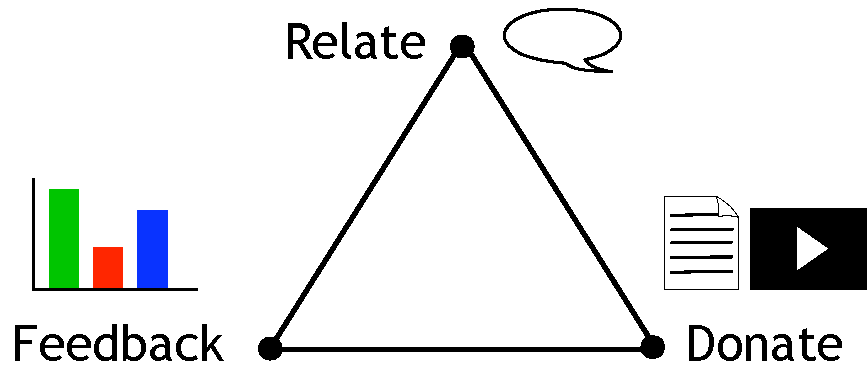
\includegraphics[width=0.33\textwidth]{figures/CollaborateSubProcesses2} 
%   \caption{Collaboration sub-activities. Designers work collaboratively in a continuum between \emph{donating}, \emph{relating}, and gathering \emph{feedback}.}
%   \label{fig:collaborate:sub:activities}
%\end{figure}

%\subsection{Challenge - Distributed Haptics}

%However, collaboration in the remote or asynchronous case is more challenging.
%Haptics has long been examined in remote collaboration both with force feedback \cite{Kim2004} and tactile \cite{Chan2008} mechanisms.
%Remote collaboration to support haptics, on the other hand, is a different beast.

%\subsubsection{Asynchronous collaboration}
%Collocated collaboration is common and well supported in haptics.
%In the synchronous case, \emph{relating} is a common activity, e.g., getting labmates and visitors to quickly try a prototype. User studies typically occur
%face-to-face as well, and 
%demonstrations at conferences \emph{donate} haptics to the community (indeed, the haptics community prioritizes demos so much that the inaugural Asia Haptics conference in 2014 was entirely in demo format).
%Asynchronous collaboration is less typical, with special advantages and issues.
%More investigation into asynchronous collaboration could reap rewards of self-running demos and user studies that collect copious data from diverse deployments % result in self-running demos and user studies that collect large amount of data from diverse populations (by deployment into different areas) 
%at low time cost to HaXD practitioners.
%%While more formal activities like feedback or donation could also be imagined , asynchronous collaboration is \kmC{get more specific : poorly understood}.
%%(self-running user studies or tactile installations \cite{Laaksolahti2011})

%\subsubsection{Distributed collaboration}
%Working remotely is even more challenging, both for synchronous and asynchronous contexts.
%Haptics involves physical devices and is a proximal sense.
%When working at a distance, there must be two identical devices.
%This means all components must be identical, whether electrical (e.g., amplifier settings), mechanical (e.g., joint dampening), or software.
%
%Distributed \textit{relating} can be supported in some small-scale cases.  % because of the small scale of devices.
%Each colleague could have a calibrated, identical device with synchronized software.
%% Because each colleague is expected to be 
%When each collaborator is knowledgeable about the device, video chat and email could provide sufficient support for many applications.
%Devices can be shipped or fabricated and calibrated at each location.
%While this introduces delay, slowing iteration and adding communication overhead, it is achievable.
%





%%%%%%%%%%%%
%
% SECTION: Methodology. How will we transform the above-mentioned approach into knowledge? How can we study our solutions?
%
%%%%%%%%%%%%
\section{Methodology}

Studying design process, creativity support tools, and haptic sensations is challenging and requires a robust methodology.
Our research questions seek to describe the process, strategies, and experience of \haxd, and to inform the design of supporting tools.
%As we have seen in our discussion of creativity and design support, systems of creativity tools are complex and noisy.
Our approach is to use mixed methods, as appropriate for our research questions.
We begin by using qualitative techniques to gather rich, generative data from design tools and design processes, and to inform iteration.
Through our work, we increasingly complement this data with quantitative methods, moving towards large-scale data collection for our generated theories with deployed tools.
%Furthermore, this work is an early inquiry requiring inductive models of thinking to generate theories, and the flexibility to accommodate invention as part of the inquiry, \eg letting us build tools iteratively based on participant feedback.
%As such, we turn to qualitative methodologies first and foremost, and as we gather findings, we gradually apply more hypothesis-testing-based approaches in a quantitative tradition.


\subsection{Inspiration and Perspectives}

extended mind and embodiment
Distributed cognition, embodiment, extended mind...
??

\subsection{Qualitative methodologies}
In this dissertation, we draw from the philosophical and methodological traditions of phenomenology, and the methodology of grounded theory.

Phenomenology is both a philosophical tradition and a social science methodology based upon that tradition that involves the study of subjective experience.
We use \citet{Moustakas1994} as our primary guide through both, as it focuses on practical methodological concerns but provides a strong philosophical background; \citet{Creswell2013} provided an overview of various methodologies and resources for phenomenology.
Critical components include \emph{horizonalization}, or preparing oneself to consider all of the participant's statements equally and with fresh eyes; distinguishing and synthesizing \emph{textural} descriptions, \eg the participant's verbatim explanation of the experience, with \emph{structural} description, or the analytical interpretation through psychology (or HCI) theories; and the documentation of the researcher's own experience with the phenomenon of study.
Phenomology as a methodology has been used in psychology to investigate topics ranging from visual illusions to tactile experience \cite{Richer1978, Obrist2013, Creswell2013}.

Methodologies, like phenomenology, often include a set of methods combined with their philosophical and epistemological underpinnings.
In this work, we specifically use the Stevick-Colaizzi-Keen methods as described by \citet{Moustakas1994}.
Transcripts are divided into non-overlapping, non-redundant statements about the phenomena known as Meaning Units (MUs).
This considers every statement that the participants make, and does not discount any due to bias or selective searching.
Then, MUs are clustered into emergent themes through affinity diagrams, writing and re-writing of thematic descriptions, and reflection guided by phenomenological philosophy.
We use this technique exactly in our first exploratory study (\autoref{ch:hapticinstrument}), and later combine it with Grounded Theory methods.

Grounded Theory is another well-known methodology first described by \citet{glaser1966awareness}.
We adopt the more flexible methodology described by \citet{Corbin2008}, as it allowed us to integrate with our phenomenological methods.
We principally adapt the methods used in Grounded Theory, specifically, memoing (writing about each focused quotation or MU), constant comparison (comparing each new memo and codes to previous ones), and open and axial coding (creating codes, or concepts, linking them together, then categorizing statements or observations based on codes).
This technique especially facillitated video analysis in \autoref{ch:tactileanimation} and \autoref{ch:macaron}, and allowed for quantitative count-based data and simple statistics to complement our interview-based findings.

We also note that researchers who use methods from the umbrella term ``qualitative research" often blend techniques from many methodologies.
Phenomenology and grounded theory are two such methodologies, others include hermeneutics, ethnography \cite{Moustakas1994}, ethnomethodology, and thematic analysis \cite{Ryan2003}.
For example, ethnography introduces the concept of ``thick description" \cite{}, where the research tries to use detailed, evocative language to convey a rich sense of being in the observed environment.
This technique is used more generally in observational notes and when writing up qualitative results to provide the rich data studied by qualitative methods.

\subsection{Towards quantitative methods at scale}
While some design scholars adopt qualitative techniques \cite{Schon1982,Cross2007,Cross2011}, others have developed quantitative techniques.
When studying graphic design for ads, \citet{Dow2011} used ratings by experts as well as click-through rates and other online analytics for actual deployed ads from their study.
\citet{Kulkarni2012} used MTurk to generate sketches of aliens in several conditions (of exposure to examples), then deployed another MTurk task to label each drawing with features like antennae or feet.
\citet{Lee2010a} had end-users rate graphic designs in both an in-lab study and over Mechanical Turk, and recorded time participant designers spent on each component.
These approaches allow for hypothesis testing for specific research questions, but require infrastructure unavailable to haptics, notably, crowd deployment, rating scales, and mature input tools.
In our early work, we found qualitative feedback to be sufficient while developing our understanding of how to build design tools.
Later, we begin to approach this infrastructure, using an online editor with analytic logs in Macaron (\autoref{ch:macaron}), and examining the potential for crowdsourced feedback with HapTurk (\autoref{ch:hapturk}).
While a valuable goal, large-scale quantitative feedback on \haxd remains outside the scope of this dissertation.



%%%%Unfortunately, these approaches do not scale to %\kmC{slc} % KM: seems like references to 'feedback' 'donate' etc should all be italicized because of their special sense.
%%%%formal \emph{feedback} or wide-spread \emph{donate tasks}, which typically have a large or anonymous audience with diverse % limited 
%%%%resources.
%%%%A wide-spread standardized device platform could support distribution, but given the variety of haptic effects \cite{Hayward2008}, this is extremely limiting and would tend to enforce a `lowest common denominator' effect.
%%%%Without assuming standardization, we suggest two possible solution strategies, each with tradeoffs:
%%%%accessible fabrication and device generalization.
%%%%
%%%%Fabrication methods like 3D printing are increasingly accessible. % to end-users.
%%%%%At a recent meeting with collaborators conducting 3D printing of haptic devices to a wide spread 
%%%%%\kmC{slc} % KM: following sentence confuses me, does it follow from 1st? Should there be a 'however"? Why does the complexity of haptic device manufacture fit it best for asynchronous collab - wouldn't that be better for synchro + collocated? 
%%%%However, manufacturing haptic devices is
%%%%complex, with software, moving parts,  and electronics, often requiring some assembly, best suited for asynchronous collaboration.
%%%%Furthermore, there is no guarantee that users have assembled their devices correctly.
%%%%Collaborators at a recent workshop found it difficult to verify % noted the difficulty in verifying 
%%%%system dynamics on their kit-based device in an asynchronous \textit{donate} task.
%%%%A resulting brainstorm \emph{ideated} a small calibration element to capture system dynamics, and a suite of diagnostic checks to help devices be consistent (e.g., template virtual environments with described ``correct behaviour").
%%%%%One promising area for investigation is in calibration tools to ensure remote devices are operating in similar fashion.
%%%%More advanced fabrication techniques may be able to improve this problem, producing moving parts, electronics, or other essential components.
%%%%
%%%%A second approach is to not attempt identical devices, but ensure they communicate what needs communicating.
%%%%We define device generalization in haptics as \emph{consistently reproducing intentional aspects of a haptic sensation}.
%%%%For example, a user watching a video of a force-feedback device on their phone could feel the force vector magnitude as vibration intensity (a \emph{donate} task), or a video chat could be augmented with a virtual environment rendered on force-feedback devices with different complexity.
%%%%This approach relies on partial standardization -- some sort of infrastructure is in place that facilitates constant output, for example, haptic broadcasting \cite{Cha2009}, touch TV \cite{Modhrain2001}, cinematography \cite{Danieau2014}, and tactile movies \cite{Kim2009}.
%%%%This is a challenging area, full of cross modal effects and contextual considerations (how is the user holding their phone?).
%%%%However, we think this is a promising approach while fabrication develops, especially for a \emph{donate} task in both synchronous and asynchronous interactions.
%%%
%%%
%%%
%%%
%%%\osC{SLC for HapTurk RW}
%%%%\section{Related Work}
%%%%We cover work related to VT icons and evaluation methods for VT effects, the current understanding of affective haptics, and work with Mechanical Turk in other modalities.
%%%%   %% \subsection{VT Icons}
%%%%     
%%%%		%%[change first sentence] VT effects are useful. According to previous studies, VT icons can communicate information [ref] and affect [ref]. VT effects are developed to assist visually-impaired users in outdoor scenarios [ref] as well as accessing digital information [ref]. In addition, VT effects can increase performance on visual interfaces, enhance engagement with the content and provide better user experience with electronic devices [ref to levesque].
%%%%		
%%%%\subsection{Existing Evaluation Methods for VT Effects} 
%%%%
%%%%The haptic community has appropriated or developed many types of user studies to evaluate VT effects and support VT design.
%%%%These target a variety of objectives:
%%%%
%%%%1) {\em Perceptibility:} Determine the perceptual threshold or Just Noticeable Difference (JND) of VT parameters. Researchers vary the values of a VT parameter (e.g., frequency)
%%%%% in small steps
%%%%to determine the minimum perceptible change
%%%%%for the parameter
%%%%~\cite{JNDstudy,foundationsoftactile}. 
%%%%
%%%%2) {\em Illusions:} Studies investigate effects like masking or apparent motion of VT sensations, useful to expand a haptic designer's palette \cite{Hayward2008,Israr2011a,Seo2013}.
%%%%
%%%%3) {\em Perceptual organization:} Reveal the underlying dimensionality of how humans perceive VT effects (which are generally different than the machine parameters used to generate the stimuli).
%%%%Multidimensional Scaling (MDS) studies are common, inviting participants compare or group vibrations based on perceived similarity~\cite{Hollins93,van2003distilling,Pasquero2006,Chan2008,Ternes2008}.
%%%%
%%%%4) {\em Encoding abstract information:} Researchers examine salient and memorable VT parameters (e.g. energy, rhythm) as well as the number of VT icons that people can remember and attribute to an information piece~\cite{Brown2006a,Allen2005,Chan2008,Ternes2008}.
%%%%
%%%%5) {\em Assign affect:} Studies investigate the link between affective characteristics of vibrations (e.g., pleasantness, urgency) to their engineering parameters (e.g., frequency, waveform)~\cite{Ternes2008,affect2015,Raisamo,Koskinen}.
%%%%To achieve this, VT researchers commonly design or collect a set of vibrations and ask participants to rate them on a set of qualitative metrics.
%%%%
%%%%6) {\em Identify language:} Participants describe or annotate tactile stimuli in natural language~\cite{Chan2008,Ternes2008,Obrist2013,Guest2011,Hwang2011,Seifi2015}.
%%%%
%%%%7) {\em Use case support:} Case studies focus on conveying information with VT icons such as collaboration~\cite{Chan2008}, public transit~\cite{Brunet2013a} and direction \cite{Brunet2013a,Arab2015}, or timing of a presentation~\cite{presentationtiming}. In other cases, VT effects are designed for user engagement, for example in games and movies, multimodal storytelling, or art installations~\cite{Israr2014,feelcraft}. 
%%%%Here, the designers use iterative design and user feedback (qualitative and quantitative with user rating) to refine and ensure effective design.
%%%%
%%%%All of the above studies would benefit from the large number of participants and fast data collection on MTurk.
%%%%In this paper, we chose our methodology so that the results are informative for a broad range of these studies.
%%%%
%%%%\subsection{Affective Haptics}
%%%%VT designers have the challenge of creating perceptually salient icon sets that convey meaningful content. A full range of expressiveness means manipulating not only 
%%%%a vibration's physical characteristics but also its perceptual and %affective
%%%%emotional properties, and collecting feedback on this. Here, we refer to all these properties as affective characteristics. 
%%%%
%%%%%;then, based on Multi-Dimensional Scaling... to 
%%%%%(New sentence)Using Multi-Dimensional Scaling (MDS) analysis of similarity ratings, it was proposed... (the same)
%%%%Some foundations for affective VT design are in place. Studies on tactile language and affect are establishing a set of perceptual metrics~\cite{Obrist2013,Seifi2015}. Guest \etal\ collated a large list of emotion and sensation words describing tactile stimuli; then, based on multidimensional scaling of similarity ratings, proposed comfort or pleasantness and arousal as key dimensions for tactile emotion words, and rough/smooth, cold/warm, and wet/dry for sensation~\cite{Obrist2013}.
%%%%Even so, there is not yet agreement on an affective tactile design language~ \cite{Jansson-Boyd2011}.
%%%%
%%%
%%%%
%%%% THIS PART MAY BE INCLUDED ALREADY IN ch:hapturk
%%%%
%%%%%Recently, Seifi \etal\ compiled research on tactile language into five taxonomies for describing vibrations~\cite{Seifi2015}.  \textbf{1) Physical properties} that can be measured: e.g., duration, energy, tempo or speed, rhythm structure; 
%%%%%\textbf{2) sensory properties}: roughness, and sensory words from  Guest \etal's touch dictionary \cite{Guest2011};
%%%%%\textbf{3) emotional interpretations}: pleasantness, arousal (urgency), dictionary emotion words \cite{Guest2011};
%%%%%\textbf{4) metaphors} provide familiar examples resembling the vibration's feel: heartbeat, insects;
%%%%%\textbf{5) usage examples} describe % types of 
%%%%%events which a vibration fits: an incoming message or alarm.
%%%%%
%%%%%%addressing Karon's comment a bit 
%%%%%%To evaluate our vibration proxies, we derived the five most salient metrics from these taxonomies. 
%%%%%To evaluate our vibration proxies, we derived six metrics from these taxonomies to capture vibrations' physical, sensory and emotional aspects:  
%%%%%1) duration, 2) energy, 3) speed, 4) roughness, 5) pleasantness, and 6) urgency. 
%%%%%% \kmC{why these 5? you took one from each taxonmy, but why this particular one?}
%%%%%
%%%%%
%%%%%\subsection{Mechanical Turk (MTurk)}
%%%%%MTurk is a platform for receiving feedback from a large number of users, in a short time at a low cost~\cite{mutrkgeneral,visualperceptionturk}. These large, fast, cheap samples have proved useful for many cases including running perceptual studies~\cite{visualperceptionturk}, developing taxonomies~\cite{taxonomyturk}, feedback on text \cite{Siangliulue2015}, graphic design \cite{Xu2014}, and sonic imitations \cite{Cartwright2015}.
%%%%%
%%%%%\purple{Crowdsourced studies have drawbacks. The  remote, asynchronous study environment is not controlled; compared to a quiet lab, participants may be subjected to unknown interruptions, and may spend less time on task with more response variability~\cite{mutrkgeneral}.
%%%%%MTurk is not suitable for getting rich, qualitative feedback or following up on performance or strategy~\cite{behavioralturk}. Best practices -- e.g., simplifying tasks to be confined to a singular activity, or using instructions complemented with example responses -- are used to reduce task ambiguity and improve response quality~\cite{Amazon.comInc.2015}.
%%%%%Some participants try to exploit the service for personal profit, exhibiting low task engagement~\cite{Downs2010}, and must be pre- or post-screened.} 
%%%%%
%%%%%Studies have examined MTurk result validity in other domains. 
%%%%%Most relevantly, Heer \etal~\cite{visualperceptionturk} validated MTurk data for graphical perception experiments (spatial encoding and luminance contrast) by replicating previous perceptual studies on MTurk. %The studies yielded similar design guidelines, albeit with greater variability; participant environment, i.e. operation system and graphical display as identified by Javascript, was a factor.
%%%%%% Further, they found the operation system and monitor details, as recorded by Javascript, a predictor of the results. 
%%%%%%\kmC{OS:slc} % KM 01.07: don't understand previous sentence. I tried to rephrase it, but I still am unsure how the environment played into the results. It seems like this counters the point of previous point: the system the subject used was a noise source, which would have gotten in way of validation.
%%%%%Similarly, we compare results of our local user study with an MTurk study to assess viability of running VT studies on MTurk, and collect and examine phone properties in our MTurk deployment. 
%%%%%%Need for Haptic Turk... that's not our title so can we use this? 
%%%%%
%%%%%{\it Need for HapTurk:} Our present goal is to give the haptic design community access to crowdsourced evaluation so we can establish modality-specific methodological tradeoffs.
%%%%%%
%%%%%There is ample need for huge-sample haptic evaluation. User experience of transmitted sensations must be robust to receiving device diversity.
%%%%%Techniques to broadcast haptic effects to video \cite{Modhrain2001,Kim2009}, e.g., with YouTube \cite{AbdurRahman2010} or MPEG7 \cite{Eid2006,Ferre2008} now require known high-fidelity devices  because of remote device uncertainty;  
%%%%%the same applies to social protocols developed for remote use of high-quality vibrations, e.g. in collaborative turn taking \cite{Chan2008}. 
%%%%%Elsewhere, studies of VT use in consumer devices need larger samples: e.g., 
%%%%%perceivability~\cite{Kaaresoja2005}, encoding of caller parameters \cite{Brown2006b}, including caller
%%%%%emotion and physical presence collected from pressure on another handset~\cite{Hoggan2012}, and usability of expressive, customizable VT icons in social messaging~\cite{Israr2015}.
%%%%%%
%%%
%%%
%%%\subsection{Mechanical Turk (MTurk)}
%%%MTurk is a platform for receiving feedback from a large number of users, in a short time at a low cost~\cite{mutrkgeneral,visualperceptionturk}. These large, fast, cheap samples have proved useful for many cases including running perceptual studies~\cite{visualperceptionturk}, developing taxonomies~\cite{taxonomyturk}, feedback on text \cite{Siangliulue2015}, graphic design \cite{Xu2014}, and sonic imitations \cite{Cartwright2015}.
%%%
%%%\purple{Crowdsourced studies have drawbacks. The  remote, asynchronous study environment is not controlled; compared to a quiet lab, participants may be subjected to unknown interruptions, and may spend less time on task with more response variability~\cite{mutrkgeneral}.
%%%MTurk is not suitable for getting rich, qualitative feedback or following up on performance or strategy~\cite{behavioralturk}. Best practices -- e.g., simplifying tasks to be confined to a singular activity, or using instructions complemented with example responses -- are used to reduce task ambiguity and improve response quality~\cite{Amazon.comInc.2015}.
%%%Some participants try to exploit the service for personal profit, exhibiting low task engagement~\cite{Downs2010}, and must be pre- or post-screened.} 
%%%
%%%Studies have examined MTurk result validity in other domains. 
%%%Most relevantly, Heer \etal~\cite{visualperceptionturk} validated MTurk data for graphical perception experiments (spatial encoding and luminance contrast) by replicating previous perceptual studies on MTurk. %The studies yielded similar design guidelines, albeit with greater variability; participant environment, i.e. operation system and graphical display as identified by Javascript, was a factor.
%%%% Further, they found the operation system and monitor details, as recorded by Javascript, a predictor of the results. 
%%%%\kmC{OS:slc} % KM 01.07: don't understand previous sentence. I tried to rephrase it, but I still am unsure how the environment played into the results. It seems like this counters the point of previous point: the system the subject used was a noise source, which would have gotten in way of validation.
%%%Similarly, we compare results of our local user study with an MTurk study to assess viability of running VT studies on MTurk, and collect and examine phone properties in our MTurk deployment. 
%%%%Need for Haptic Turk... that's not our title so can we use this? 
%%%
%%%
%%%
%%%%Hapturk
%%%Recently, Seifi \etal\ compiled research on tactile language into five taxonomies for describing vibrations~\cite{Seifi2015}.  \textbf{1) Physical properties} that can be measured: e.g., duration, energy, tempo or speed, rhythm structure; 
%%%\textbf{2) sensory properties}: roughness, and sensory words from  Guest \etal's touch dictionary \cite{Guest2011};
%%%\textbf{3) emotional interpretations}: pleasantness, arousal (urgency), dictionary emotion words \cite{Guest2011};
%%%\textbf{4) metaphors} provide familiar examples resembling the vibration's feel: heartbeat, insects;
%%%\textbf{5) usage examples} describe % types of 
%%%events which a vibration fits: an incoming message or alarm.
%%%
%%%


%%%
%
% END
%
\endinput

%Any text after an \endinput is ignored.
%You could put scraps here or things in progress.


% $Id: template.tex 11 2007-04-03 22:25:53Z jpeltier $

%\documentclass{vgtc}                          % final (conference style)
%%\documentclass[review]{vgtc}                 % review
%%\documentclass[widereview]{vgtc}             % wide-spaced review
%%\documentclass[preprint]{vgtc}               % preprint
%%\documentclass[electronic]{vgtc}             % electronic version
%
%% Added by KM, 130928, to get it to compile. Not sure why.
%\let\ifpdf\relax
%
%
%%% Uncomment one of the lines above depending on where your paper is
%%% in the conference process. ``review'' and ``widereview'' are for review
%%% submission, ``preprint'' is for pre-publication, and the final version
%%% doesn't use a specific qualifier. Further, ``electronic'' includes
%%% hyperreferences for more convenient online viewing.
%
%%% Please use one of the ``review'' options in combination with the
%%% assigned online id (see below) ONLY if your paper uses a double blind
%%% review process. Some conferences, like IEEE Vis and InfoVis, have NOT
%%% in the past.
%
%%% Figures should be in CMYK or Grey scale format, otherwise, colour 
%%% shifting may occur during the printing process.
%
%%% These three lines bring in essential packages: ``mathptmx'' for Type 1 
%%% typefaces, ``graphicx'' for inclusion of EPS figures. and ``times''
%%% for proper handling of the times font family.
%
%\usepackage{mathptmx}
%\usepackage{graphicx}
%\usepackage{times}
%
%% K additions (commenting)
%\usepackage{xcolor}
%%\usepackage{pdfcomment}
%
%%% We encourage the use of mathptmx for consistent usage of times font
%%% throughout the proceedings. However, if you encounter conflicts
%%% with other math-related packages, you may want to disable it.
%
%%% If you are submitting a paper to a conference for review with a double
%%% blind reviewing process, please replace the value ``0'' below with your
%%% OnlineID. Otherwise, you may safely leave it at ``0''.
%\onlineid{0}
%
%%% declare the category of your paper, only shown in review mode
%\vgtccategory{Research}
%
%%% allow for this line if you want the electronic option to work properly
%\vgtcinsertpkg
%
%
%% sort citations
%\usepackage{cite}
%%\usepackage[sort]{natbib}
%
%
%%% =================================
%% inline comments[KM addition]
%\definecolor{DarkGreen}{rgb}{0.0, 0.6, 0.0}
%\definecolor{DarkRed}{rgb}{0.7, 0.2, 0.2}
%\definecolor{DarkMagenta}{rgb}{0.5, 0.0, 0.5}
%\definecolor{DarkCyan}{rgb}{0.0, 0.6, 0.6}
%
%%\newcommand{\inlinecomment}[3][]{$\lceil$\textbf{#1}~\textit{\textcolor{#2}{#3}}$\rfloor$}
%\newcommand{\inlinecomment}[3][]{\textbf{#1}~\textit{\textcolor{#2}{#3}}}
%
%\newcommand{\todo}[1]{\noindent \inlinecomment[TODO]{DarkRed}{#1}}
%\newcommand{\km}[1]{\noindent \inlinecomment{DarkGreen}{#1}}
%\newcommand{\ikComment}[1]{\noindent \inlinecomment[IK]{DarkCyan}{#1}}
%\newcommand{\bgComment}[1]{\noindent \inlinecomment[BG]{blue}{#1}}
%
%
%\newcommand{\kmEdit}[1]{\textcolor{DarkGreen}{#1}}
%% \newcommand{\grn}[1]{\textcolor{DarkGreen}{#1}}
%%% =================================
%
%

\chapter{Sketch: The Haptic Instrument}
\label{ch:hapticinstrument}


%% In preprint mode you may define your own headline.
%\preprinttext{To appear in an IEEE VGTC sponsored conference.}

%% Paper title.

%\title{Haptic Jazz: Designing Touch with the Haptic Instrument}
%\title{Improvising Design with a Haptic Instrument}

%% This is how authors are specified in the conference style

%% Author and Affiliation (single author).
%%\author{Roy G. Biv\thanks{e-mail: roy.g.biv@aol.com}}
%%\affiliation{\scriptsize Allied Widgets Research}

%% Author and Affiliation (multiple authors with single affiliations).
%%\author{Roy G. Biv\thanks{e-mail: roy.g.biv@aol.com} %
%%\and Ed Grimley\thanks{e-mail:ed.grimley@aol.com} %
%%\and Martha Stewart\thanks{e-mail:martha.stewart@marthastewart.com}}
%%\affiliation{\scriptsize Martha Stewart Enterprises \\ Microsoft Research}

%% Author and Affiliation (multiple authors with multiple affiliations)
\author{Oliver S. Schneider\thanks{e-mail: oschneid@cs.ubc.ca} \qquad \qquad Karon E. MacLean\thanks{e-mail: maclean@cs.ubc.ca}\\ %
        \scriptsize Department of Computer Science \\
        \scriptsize University of British Columbia, Vancouver, Canada
}
%\author{Oliver S. Schneider\thanks{e-mail: oschneid@cs.ubc.ca}\\ %
%        \scriptsize University of British Columbia %
%\and Karon E. MacLean \thanks{e-mail: maclean@cs.ubc.ca}\\ %
%        \scriptsize University of British Columbia %
%%\and Martha Stewart\thanks{e-mail:martha.stewart@marthastewart.com}\\ %
%%     \parbox{1.4in}{\scriptsize \centering Martha Stewart Enterprises \\ Microsoft Research}
%}

%% A teaser figure can be included as follows, but is not recommended since
%% the space is now taken up by a full width abstract.
%\teaser{
%  \includegraphics[width=1.5in]{sample.eps}
%  \caption{Lookit! Lookit!}
%}

%%\abstract{
%% Designing haptic phenomena is increasingly important but difficult.
%As the need to deploy informative, expressive haptic phenomena in consumer devices gains momentum, the inadequacy of current design tools is becoming more critically obstructive.
%%However, this increased activity  also makes it possible to characterize issues, and address them with advances in software engineering.
%%Designers face two primary obstacles.
%Current tools do not support collaboration or serendipitous exploration.
%Collaboration is critical,
%but direct means of sharing haptic sensations are limited,
%and the absence of unifying conceptual models for working with haptic sensations further restricts communication between designers and stakeholders.
%%Because there are no unifying conceptual models for working with haptic sensations, there are major communication problems between designers and stakeholders.
%%: neither designers, nor managers, nor users can articulate what they experience.
%%This is especially troublesome when designing pleasant, affective interactions that rely upon user experience.
%This is especially troublesome for pleasurable, affectively targeted interactions that rely on 
%subjective user experience.
%%In this paper, we introduce our solution: the haptic instrument, analogous to a musical instrument, a new tool for real-time, collaborative manipulation of haptic sensations.
%In this paper, we introduce an alternative design approach
%inspired by musical instruments -- a new tool for real-time, collaborative manipulation of haptic sensations;
%and describe % the design of 
%a first example, mHIVE, a mobile Haptic Instrument for Vibrotactile Exploration.
%%, which allows both designers and users to express vibrotactile \km{(VT)} ideas with a simple touchscreen interface.
%Our qualitative study shows that mHIVE supports exploration and communication but
%requires additional visualization and recording capabilities for tweaking designs,
%and expands previous work on haptic language.
%%and reveals future research directions for both design tools and language.
%%}


%% ACM Computing Classification System (CCS). 
%% See <http://www.acm.org/class/1998/> for details.
%% The ``\CCScat'' command takes four arguments.
%
%\CCScatlist{
%  \CCScat{H.5.2}{Information Interfaces and Presentation (e.g., HCI)}{User Interfaces}{Haptic I/O}
%}

%% Copyright space is enabled by default as required by guidelines.
%% It is disabled by the 'review' option or via the following command:
% \nocopyrightspace

%%%%%%%%%%%%%%%%%%%%%%%%%%%%%%%%%%%%%%%%%%%%%%%%%%%%%%%%%%%%%%%%
%%%%%%%%%%%%%%%%%%%%%% START OF THE PAPER %%%%%%%%%%%%%%%%%%%%%%
%%%%%%%%%%%%%%%%%%%%%%%%%%%%%%%%%%%%%%%%%%%%%%%%%%%%%%%%%%%%%%%%%

% Make sure hyperref comes last of your loaded packages, 
% to give it a fighting chance of not being over-written, 
% since its job is to redefine many LaTeX commands.
%\usepackage[pdftex]{hyperref}
%\hypersetup{
%pdftitle={SIGCHI Conference Proceedings Format},
%pdfauthor={LaTeX},
%pdfkeywords={SIGCHI, proceedings, archival format},
%bookmarksnumbered,
%pdfstartview={FitH},
%colorlinks,
%citecolor=black,
%filecolor=black,
%linkcolor=black,
%urlcolor=black,
%breaklinks=true,
%}


%Set graphics path

%% create a shortcut to typeset table headings
%\newcommand\tabhead[1]{\small\textbf{#1}}
%
%%new command that is a bold item
\newcommand\strongitem[1]{{\textbf{#1.}}}
%
%%new command that describes a theme:
\newcounter{themecounter}
\stepcounter{themecounter}
%%\newcommand\theme[1]{\vspace{2mm}\textbf{Theme \thethemecounter: #1}\stepcounter{themecounter}}
%%\newcommand\theme[1]{\subsection{Theme \thethemecounter: #1}\stepcounter{themecounter}}
\newcommand\theme[1]{\subsection{#1}}

%quote commands
\newcommand\q[1]{\textit{``#1"}} 			%\q for quote
\newcommand\sq[1]{{\q{#1}}}			%\sq for small quote
\newcommand\namedquote[2]{{\q{#2} (#1)}}
%\newcommand\namedquote[2]{{\textbf{#1:} \q{#2}}}
\newcommand\nq[2]{\namedquote{P#1}{#2}}	%\nq for named quote of participant number N
\newcommand\term[1]{\textit{#1}} 			%\term

%\numberofauthors{1}
%%\author{
%%  \alignauthor Author(s) Name(s)\\
%%    \affaddr{Affiliation(s)}\\
%%    \affaddr{Address(es)}\\
%%    \email{e-mail address(es)}\\
%%    \affaddr{Optional phone number(s)}
%%}
%
%
%%\keywords{
%%	vibrotactile; design tools;
%%	\textcolor{red}{Mandatory section to be included in your final version.}
%%}
%
%%\category{H.5.m.}{Information Interfaces and Presentation (e.g. HCI)}{Miscellaneous}
%%See: \url{http://www.acm.org/about/class/1998/}
%%for more information and the full list of ACM classifiers
%%and descriptors.
%
%\begin{document}
%% The ``\maketitle'' command must be the first command after the
%% ``\begin{document}'' command. It prepares and prints the title block.

%% the only exception to this rule is the \firstsection command

%%%%%%%%%%%%%%%%%%
%
% SECTION: Introduction
% 
%%%%%%%%%%%%%%%%%%
%\section{Introduction}

%%\maketitle
%
%Haptic feedback has hit %devices  are hitting 
%the mainstream, present in smartphones, gaming and automobile design,
%%Everything from smartphones to cars are adopting higher-fidelity haptic technology.
%but our knowledge of how to design haptic phenomena remains limited.
%%Despite years of research
%There are still no agreed-upon vocabularies or conceptual models for haptic phenomena \cite{Enriquez2003,Ledo2012,Lee2009,Obrist2013}, % putting \km{us} % haptic design at a loss when compared 
%in contrast to other modalities (\emph{e.g.}, using theory of minor chords to evoke a sad emotion in music).
%% Prospects are even more limited when developing sensations to have qualitative features, such as pleasant alerts or frightening game environments.
%For subjective qualities, such as pleasant alerts or frightening game environments, prospects are even more limited.
%%
%Design is still based on trial and error with programming languages, limiting exploration.
%%Programming languages are primarily used, limiting exploration.
%The lack of established conceptual models or design frameworks further challenges communication between designers and stakeholders.
%%The subset of tactile sensations has a number of candidates (e.g., vibrotactile score \cite{Lee2009}), but even this area can be improved.
%%In particular, existing tools fail to support designers in two ways:
%
%%\begin{itemize}
%%	\item Development cycles are still based on compile, run, adjust cycles, or hardware vendor demos/examples
%%	\item There is no understood mental model or design theory when creating haptic phenomena
%%\end{itemize}
%

%\begin{figure}[th] %  figure placement: here, top, bottom, or page
%   \centering
%   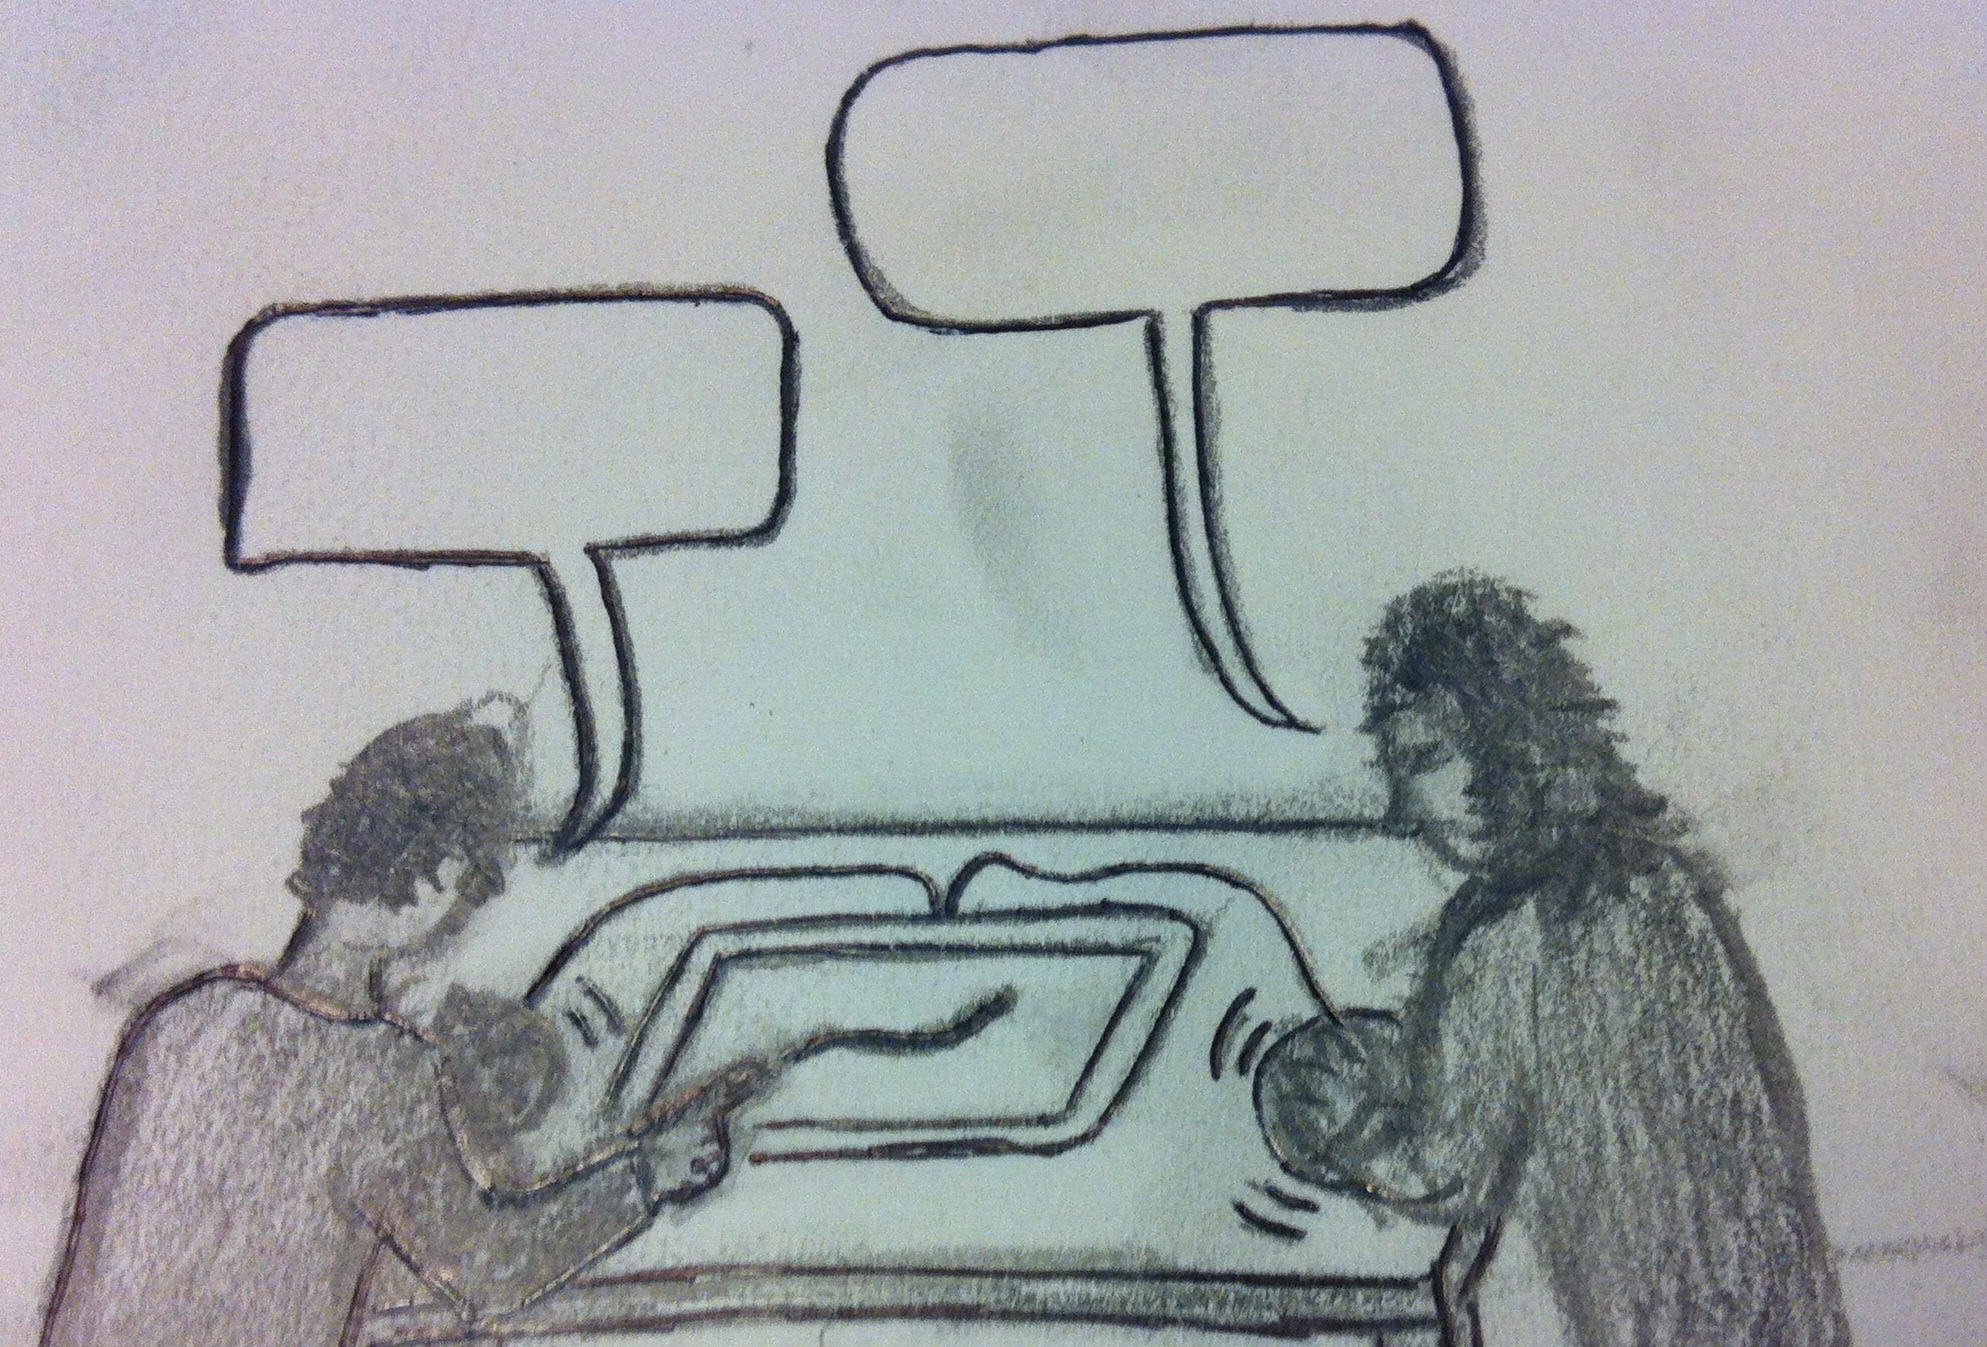
\includegraphics[width=0.4\textwidth]{HapticInstrumentConceptSketchRough} 
%   \caption{Concept Sketch of the Haptic Instrument}
%   \label{fig:HapticInstrumentConceptSketch}
%\end{figure}

\begin{figure}[h] %  figure placement: here, top, bottom, or page
   \centering
   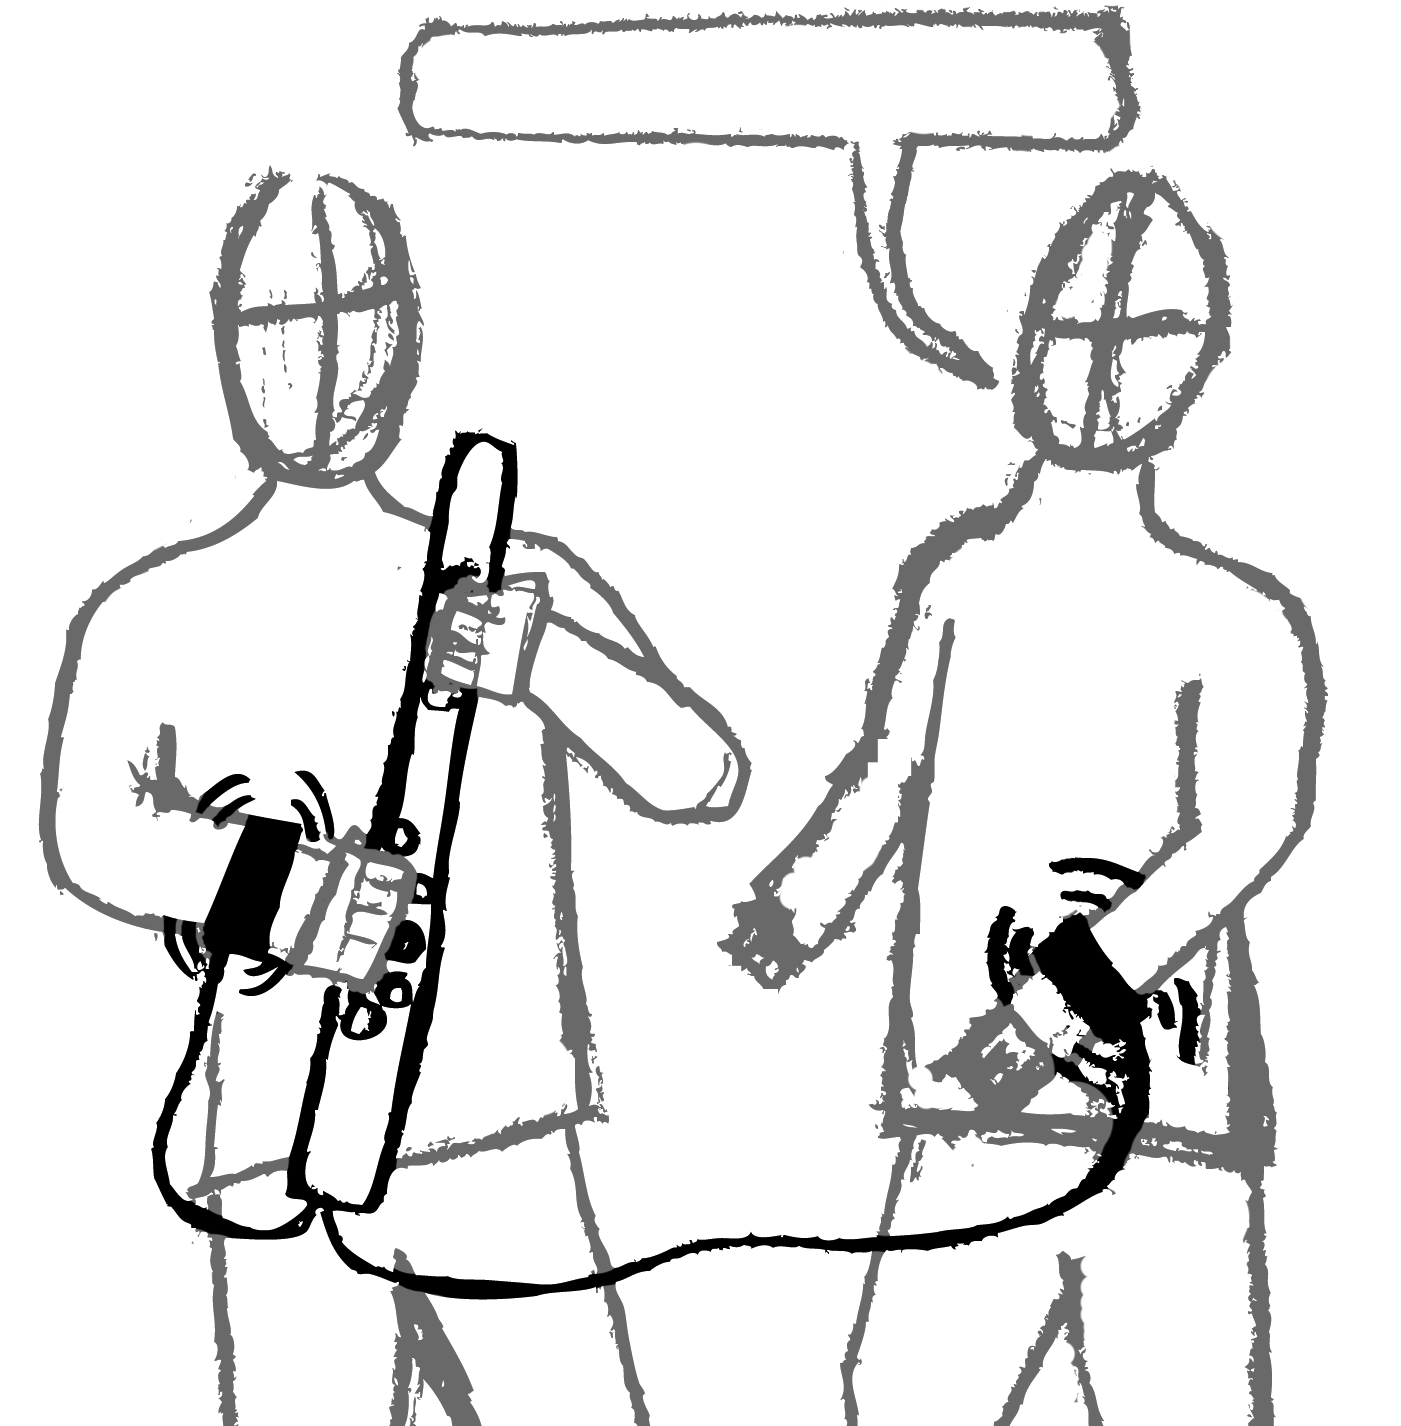
\includegraphics[width=0.5\textwidth, height=2.3in]{haptic-instrument-concept-sketch-sax-small-traced-squarer} 
   \caption{Concept sketch of a haptic instrument. Both users experience the same sensation, controlled in real-time.}
   \label{fig:HapticInstrumentConceptSketch}
\end{figure}

The Haptic Instrument case study\footnote{Published in Haptics Symposium 2014 \cite{Schneider2014} and at a CHI 2014 workshop \cite{Schneider2014b}.} is a first exploration into building a vibrotactile design tool, looking at design activities of exploration and informal sharing.
Through it, we investigate the role of real-time feedback and synchronous collaboration on haptic experience design, using participants with some haptics experience, serving as proxies for haptic experience designers.
Conventional haptic design tools contain a slow iteration, requiring programming or rendering before playback.
Using a music composition metaphor (as in~\cite{Lee2009}), we are writing music without ever playing a note: composing a work in its entirety, then listening to the result before making changes.
In contrast, musicians often use their instruments as a tool for serendipitous exploration when designing music.
%and can draw upon musical theory.
Furthermore, music is collaborative, with communication facilitated by a reference point of a sound.
%Touch, however, is a personal, local sense, making it difficult to discuss stimuli.


%Facilitated exploration and collaboration % in haptic design should 
%should streamline the haptic design process and inform a guiding 
%theory, analogous to those for musical composition. % theory. % vague?
%% With eased exploration, 
%Designers will attain fluency with new devices and control parameters,
%while collaborative elements % should help communication, but also 
%% could prove key to developing this theory.
%%Previous approaches have all been single-user design tools.
%%We suspect that adding a collaborative element is the key to developing these languages
%will get people designing in groups.  A usable haptic language may emerge from their dialogue.
%% they use to collaborate might emerge naturally from the collaborative interactions.


%Furthermore, recent work has identified major communication barriers in industry. Designers of haptic sensations are forced to carry examples of different textures or dynamical systems to make their point to stakeholders.



Our approach is to directly use a \emph{haptic instrument}, inspired by musical instruments but producing (for example) vibrotactile (VT) sensations rather than sound (\autoref{fig:HapticInstrumentConceptSketch}).
Haptic instruments are intended to have two main uses: they provide real-time feedback to the user to facilitate improvisation and exploration, and produce haptic output to multiple users as a \emph{what-you-feel-is-what-I-feel} (WYFIWIF) interface.
This allows for a dialogue that includes a haptic modality: haptic instruments create a shared experience of touch, allowing for a common reference point.


% when two or more people are talking.
%We hope that haptic instruments will not only prove to be useful tools in their own right, but also allow for a haptic language to emerge naturally from the dialogue surrounding this shared experience.
%We developed a vibrotactile instance, mHIVE (mobile Haptic Instrument for Vibrotactile Exploration), as a platform to investigate this concept.


%Our main contributions are:
%\begin {itemize}
%	\item A definition of the haptic instrument concept \& design space.
%	\item A fully-working haptic instrument (mHIVE).
%	\item The novel application of an established psychological methodology, phenomenology, to investigate mHIVE's interface and subjective tactile experiences.
%%	rather than psychophysical thresholds.
%	\item Preliminary results from a qualitative study that show mHIVE supports exploration and collaboration, and implications for the design of future haptic design tools.
%\end{itemize}

%%\noindent
%In this paper, we first cover the related work of haptic design tools and haptic language,
%%, identifying the progress so far in haptic design tools and conceptual models.
% then define the haptic instrument, its requirements, features, and design space.
%We report the design of mHIVE,
%% and the feedback we have encountered.
%our methodology, and preliminary results, and
%% investigating both the experience of using mHIVE and the language used to describe haptic phenomena.
% conclude with future directions for haptic tool design and research into a haptic language.
%%, and a vision for how haptic instruments can be used to develop a conceptual framework, the analogous musical theory for haptic sensations.
%%
%%\begin{itemize}
%%	\item Haptic jazz is a rich metaphor
%%	\item Haptic ``lead sheets" instead of scores
%%	\item improvisation
%%	\item social
%%\end{itemize}

\begin{figure*}[Htb]
   \centering
   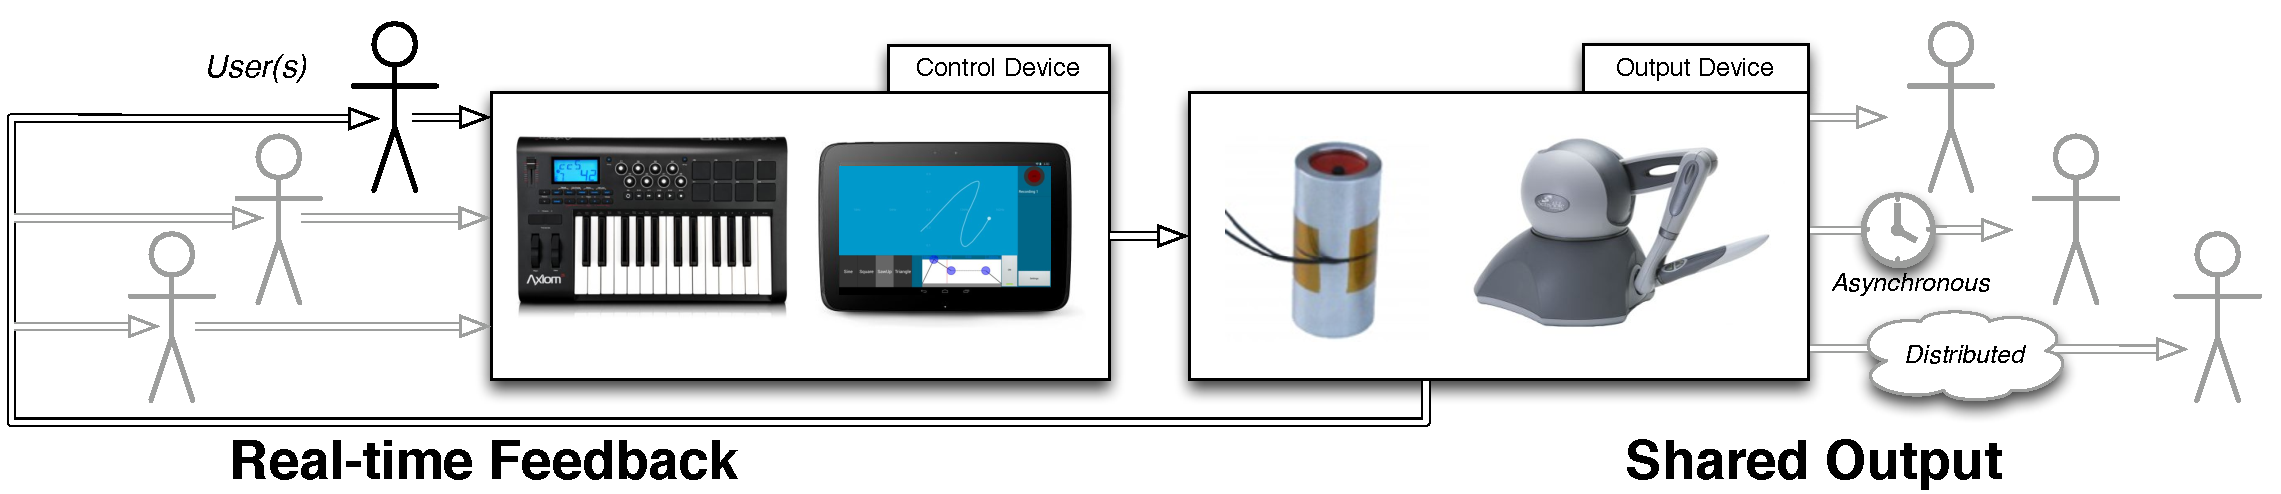
\includegraphics[width=\textwidth]{haptic-instrument-concept-horizontal4-small} 
   \caption{The haptic instrument concept. One or more people control the instrument, and receive real-time feedback from the device. Any number of audience members can feel the output in real time as well. Control methods can vary, from traditional musical control devices (such as the M-Audio Axiom 25, used in preliminary prototypes) to touchscreen tablets (used in mHIVE). Output devices vary as well.}
   \label{fig:HapticInstrumentConcept}
\end{figure*}




%Finally, we draw inspiration the Logo, which uses the ``transitionary object" of a turtle \cite{Papert1980}??? to aid users in making  to communicate experience, live coding ? Programming by example, haptic camera line of thought?


%%%%%%%%%%%%%%%%%%
%
% SECTION: Defining the Haptic Instrument
% 
%%%%%%%%%%%%%%%%%%
%\section{Defining the Haptic Instrument}
%We define a haptic instrument as a tool for general manipulation of one or more haptic (tactile, force-feedback, or both) devices that provides real-time feedback to anyone controlling the device, and can produce identical shared (WYFIWIF) output to all users to facilitate discussion and collaboration.
%Manipulation can include ideation, exploration, communication, recording, refinement, and articulation.
%Manipulation can be for utilitarian purposes (\emph{e.g.}, designing haptic notifications) or artistic expression (\emph{e.g.}, a haptic performance).
%Output devices can be purely output, or interactive.
%Furthermore, although haptic devices must be involved, multimodal experiences could easily be created by combining a haptic instrument with auditory or visual output.\footnote{One could even imagine a multimodal instrument such as Asimov's Visi-Sonor \cite{Asimov-Foundation-and-Empire} or its parody, Futurama's Holophonor \cite{Futurama-33-ParasitesLost}.}


%\begin{figure*}[htb]
%   \centering
%   \begin{minipage}{0.65\textwidth}
%	   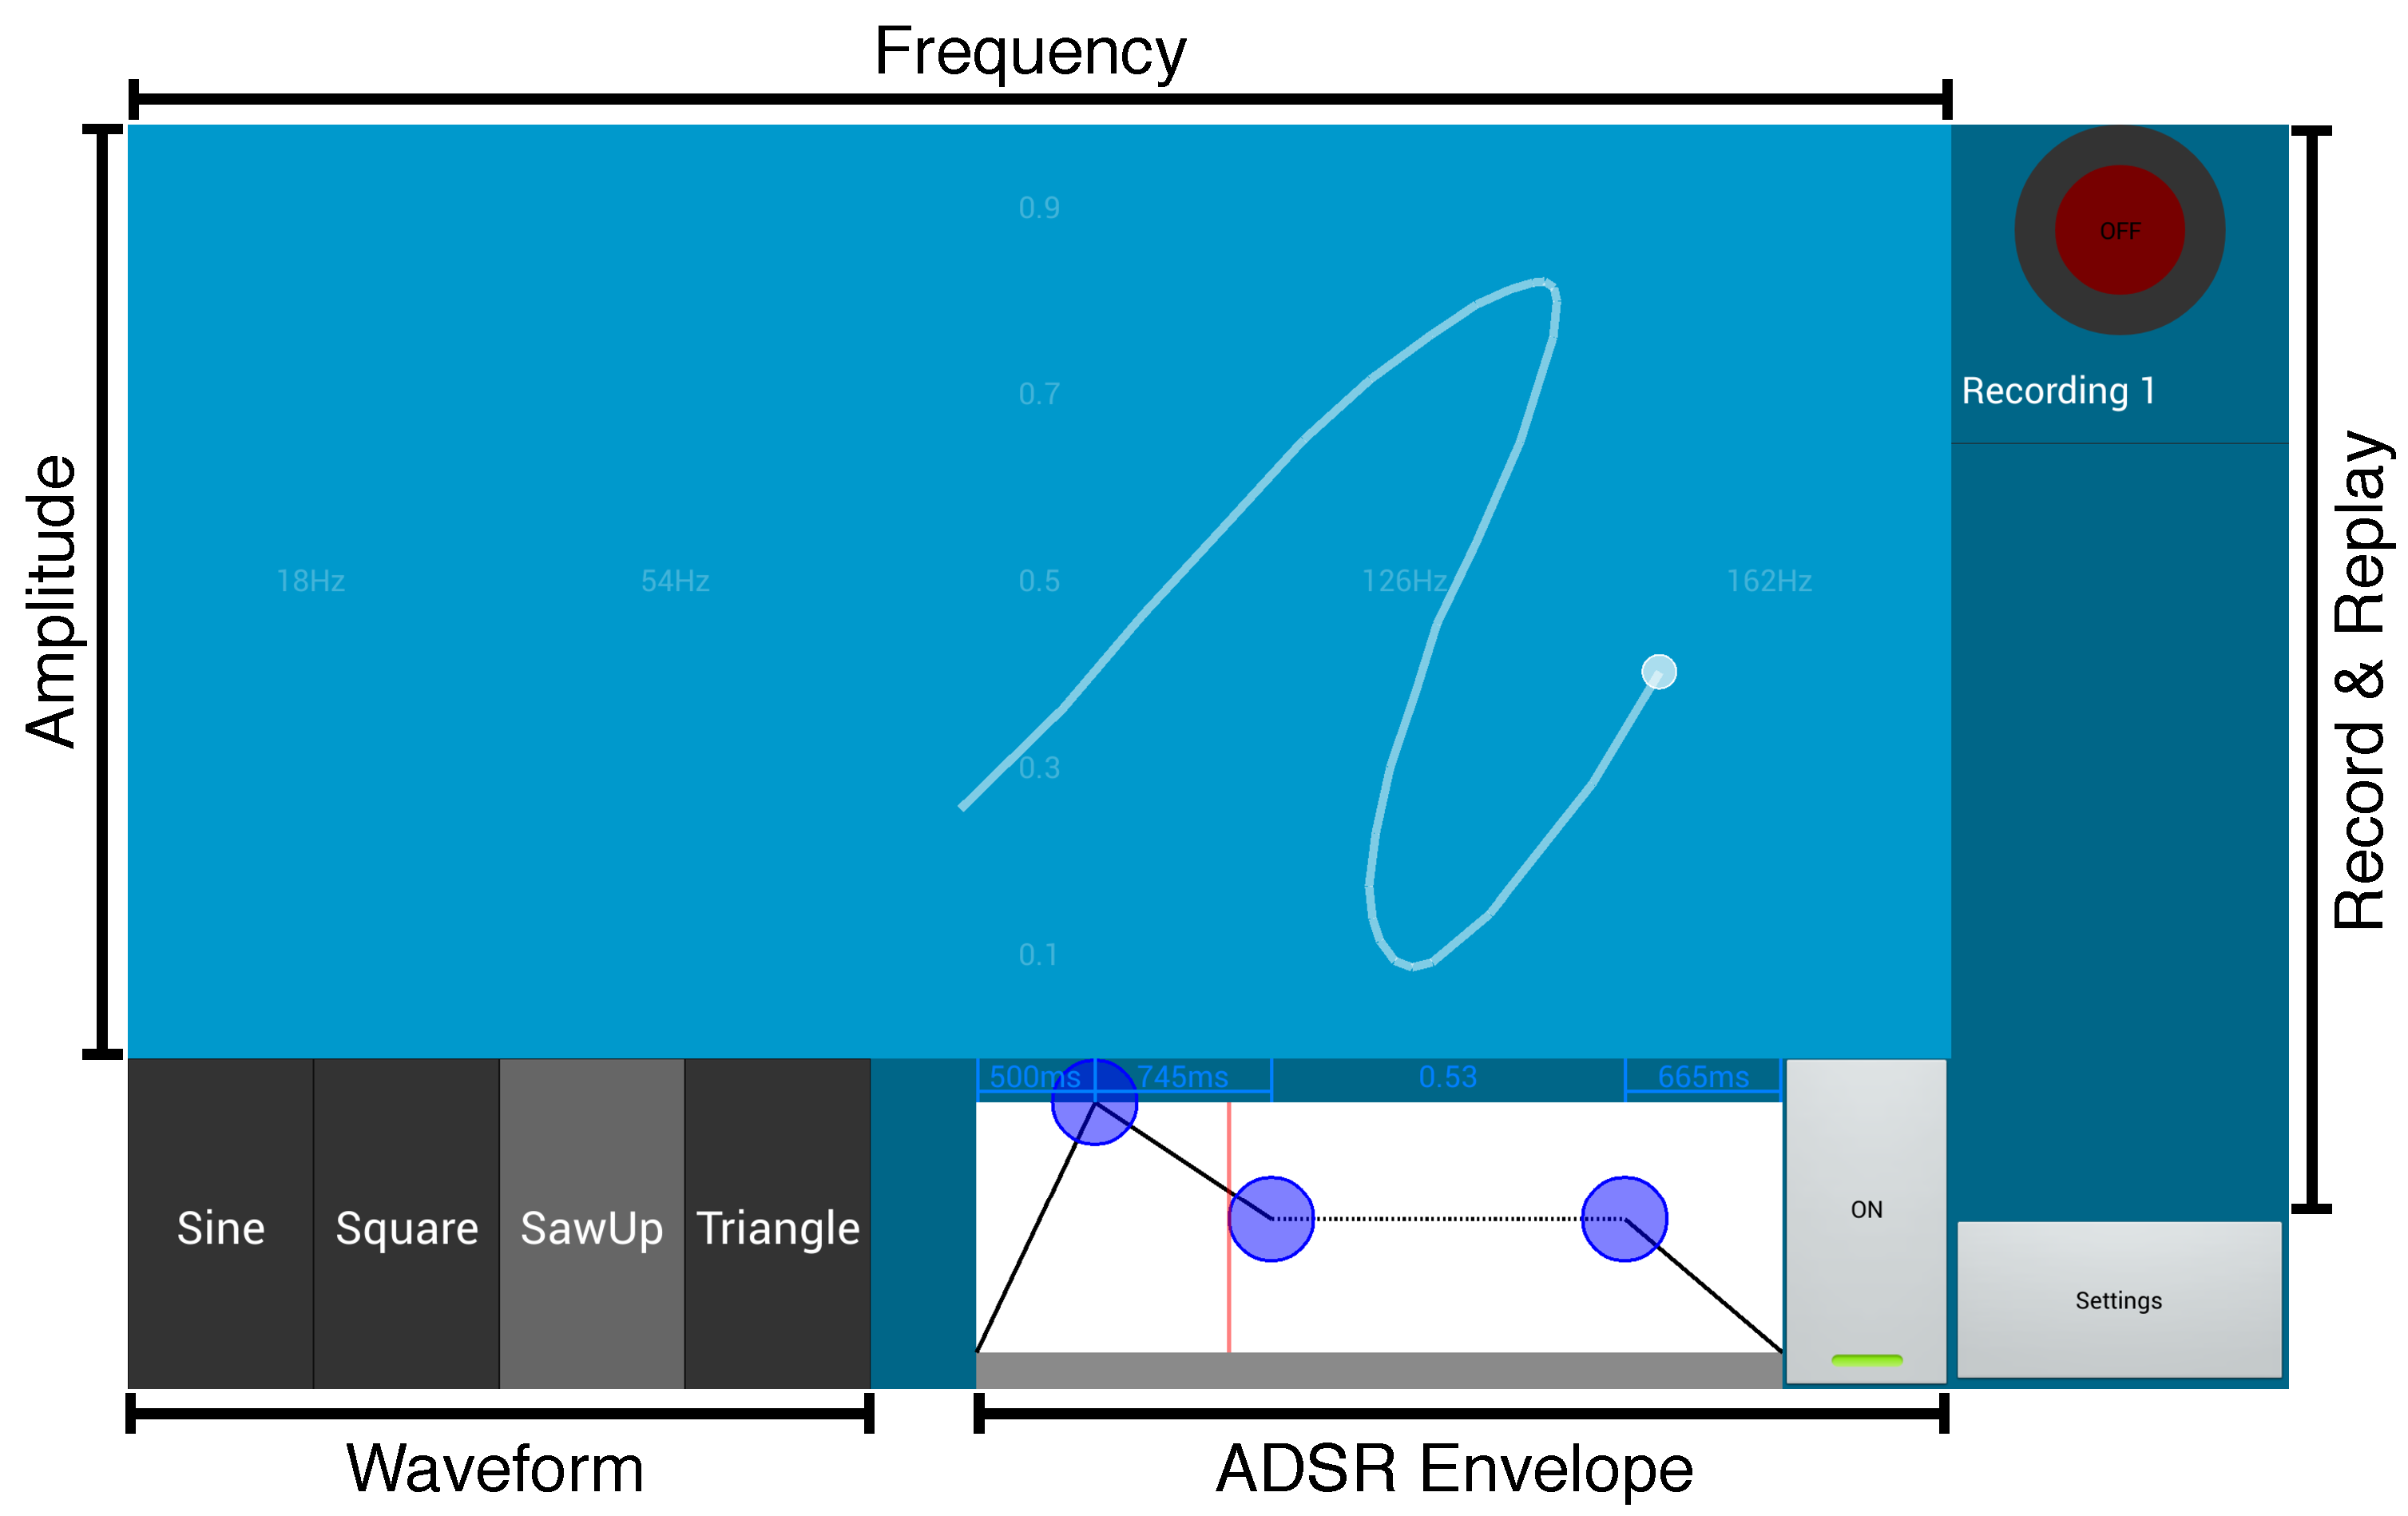
\includegraphics[width=\textwidth]{mHIVE-screenshot-labeled-2013-08-13} 
%	   \caption{mHIVE interface. Primary interaction is through the amplitude-frequency view, where visual feedback is provided through a circle (current finger position) and a trail (two seconds of previous interaction history).}
%	   \label{fig:mHIVE}
%    \end{minipage}
%    \hspace{1cm}
%   \begin{minipage}{0.25\textwidth}
%	   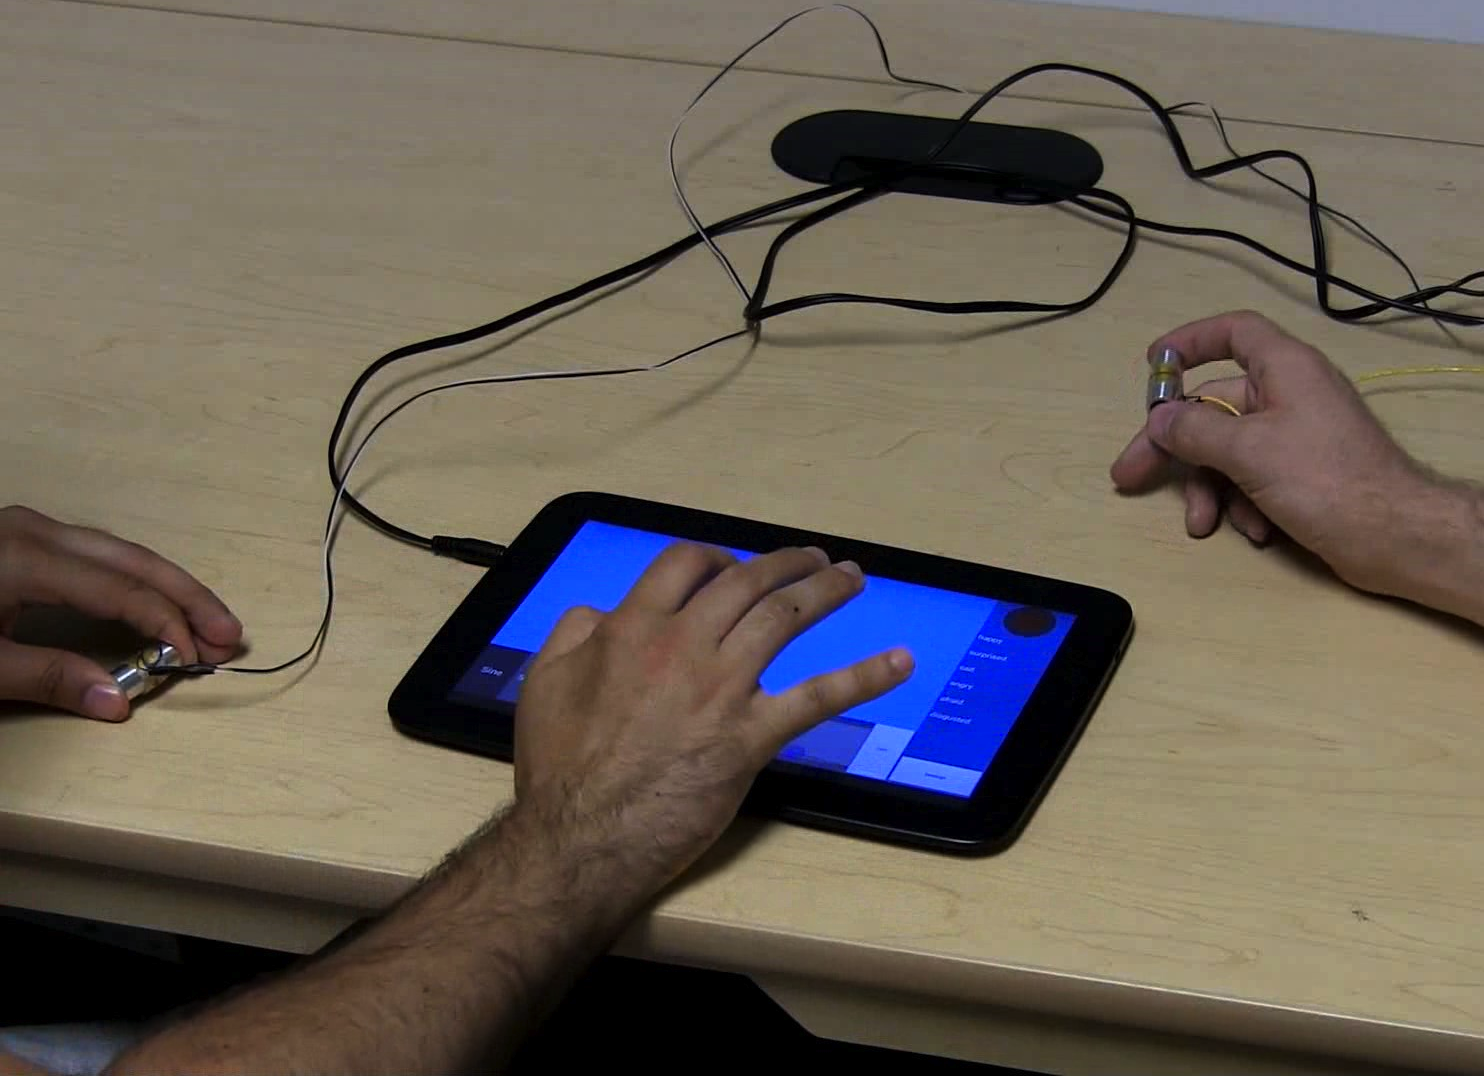
\includegraphics[width=\textwidth]{mHIVE-study-setup-cropped} 
%	   \caption{Study setup. The participant (left) controls the device while feeling the sensation; the interviewer (right) feels the same sensation on an identical output device.}
%	   \label{fig:StudySetup}
%    \end{minipage}   
%\end{figure*}





%%%%%%%%%%%%%%%%%%
%
% SECTION: mHIVE
% 
%%%%%%%%%%%%%%%%%%
\section{Design}

%%%%%
%SubSection: Design Dimensions
%%%%
%\subsection{Design Dimensions}
%Though haptic instruments by definition provide real-time feedback have shared-output, there are several main design dimensions that can be considered in a haptic instrument (outlined in \autoref{fig:HapticInstrumentConcept}).
%Note that haptic instruments can occupy multiple positions on these dimensions.
% Though haptic instruments by definition provide real-time feedback \kmEdit{??} have shared-output, 
There are several main design dimensions that can be considered in a haptic instrument (outlined in \autoref{fig:HapticInstrumentConcept}).
A haptic instrument can occupy multiple positions on these dimensions.
%; a haptic instrument could allow for both synchronous and asynchronous collaboration.

%\begin{description}

	\strongitem{Asychronous/synchronous}
%	Because of the shared-output,
%A haptic instrument collaborative.
Though a haptic instrument must provide real-time feedback, its collaborative (shared-output) aspect could be either synchronous (by having multiple people experience the real-time output) or asynchronous (by allowing for recording and playback, important for design).
%Indeed, recording is critical when creating musical pieces.

	\strongitem{Collocated/distributed} A haptic instrument's output could be present only for users in the same room, or be broadcast over a network to people around the world. For example, multiple mobile devices could all display identical output in a distributed manner.

	\strongitem{Private/shared %KM suggested collaborative, not going with it because of our use of "collaborative" elsewhere
control} A haptic instrument's control % interface 
 could be private (operated by a one person at a time) or shared (multiple users control the display). 
Shared control could be collocated or distributed (\emph{e.g.}, a web interface and shared object model).
	
	\strongitem{Output mechanism} Each haptic instrument will control a haptic device, which has its own mechanism for providing a haptic sensation (\emph{e.g.}, vibrotactile sensations). Because haptic devices can be complex and combine multiple mechanisms, this is a large space in its own right. Characterizing the different display mechanisms is something that we must leave to future work. Suffice it to say, a haptic instrument will be different depending on its output device.

	\strongitem{Number of haptic instruments or output devices}
	One consideration is whether a haptic instrument is intended to operate alone, or with other haptic or multimodal instruments.
%	\kmEdit{slc} % Don't you need to mention also, multimodal design? jam the haptic channel along with the auditory?
	One can imagine haptic jam sessions for inspiration and ideation, or even form haptic bands for artistic expression.
	This is highly related to private/shared control -- there is a fine line between several identical haptic instruments with private control, and a single haptic instrument with shared control and several output devices. Note that a haptic instrument may involve several devices to produce shared-output.

	\strongitem{Control mechanism} Similarly, a haptic instrument could be controlled in a variety of ways.
	From musically-inspired MIDI controllers to smartphone applications, we envision a wide variety of control methods.
%	Even a real-time programming environment might be appropriate for complex interactive sensations.
%	One should note that the control mechanism must work with the output device's paradigm.
	Even a real-time programming environment might be appropriate for complex interactive sensations,
	so long as the control mechanism works with the output device's paradigm.
%	 likely depend on the display mechanism, as many display mechanisms required their own paradigm for control.

%\end{description}
%
%We expect that haptic instruments could provide both immediate and long-term value.
%% In the short term, 
%We hope haptic instruments will improve the design process immediately, by supporting exploration and collaboration.
%% won't just be valuable on their own, but might produce emergent value.
%%We also expect that there will be other valuable results that are emergent from.
%%We expect that exploration will help designers quickly internalize the meaning of different control parameters for a given device.
%%of different display mechanisms and the parallel differences in control paradigms.
%%Collaboration, on the other hand, could develop an explicit conceptual model or language analogous to musical theory that could aid haptic designers.
%Over time, their use could lead to a natural, emergent design language valuable in its own right.
%One can also imagine a general tool composed of several virtual haptic instruments, much like digital musical synthesizers.
%
%%User stories, requirements?

\begin{figure}[Htb]
   \centering
%	   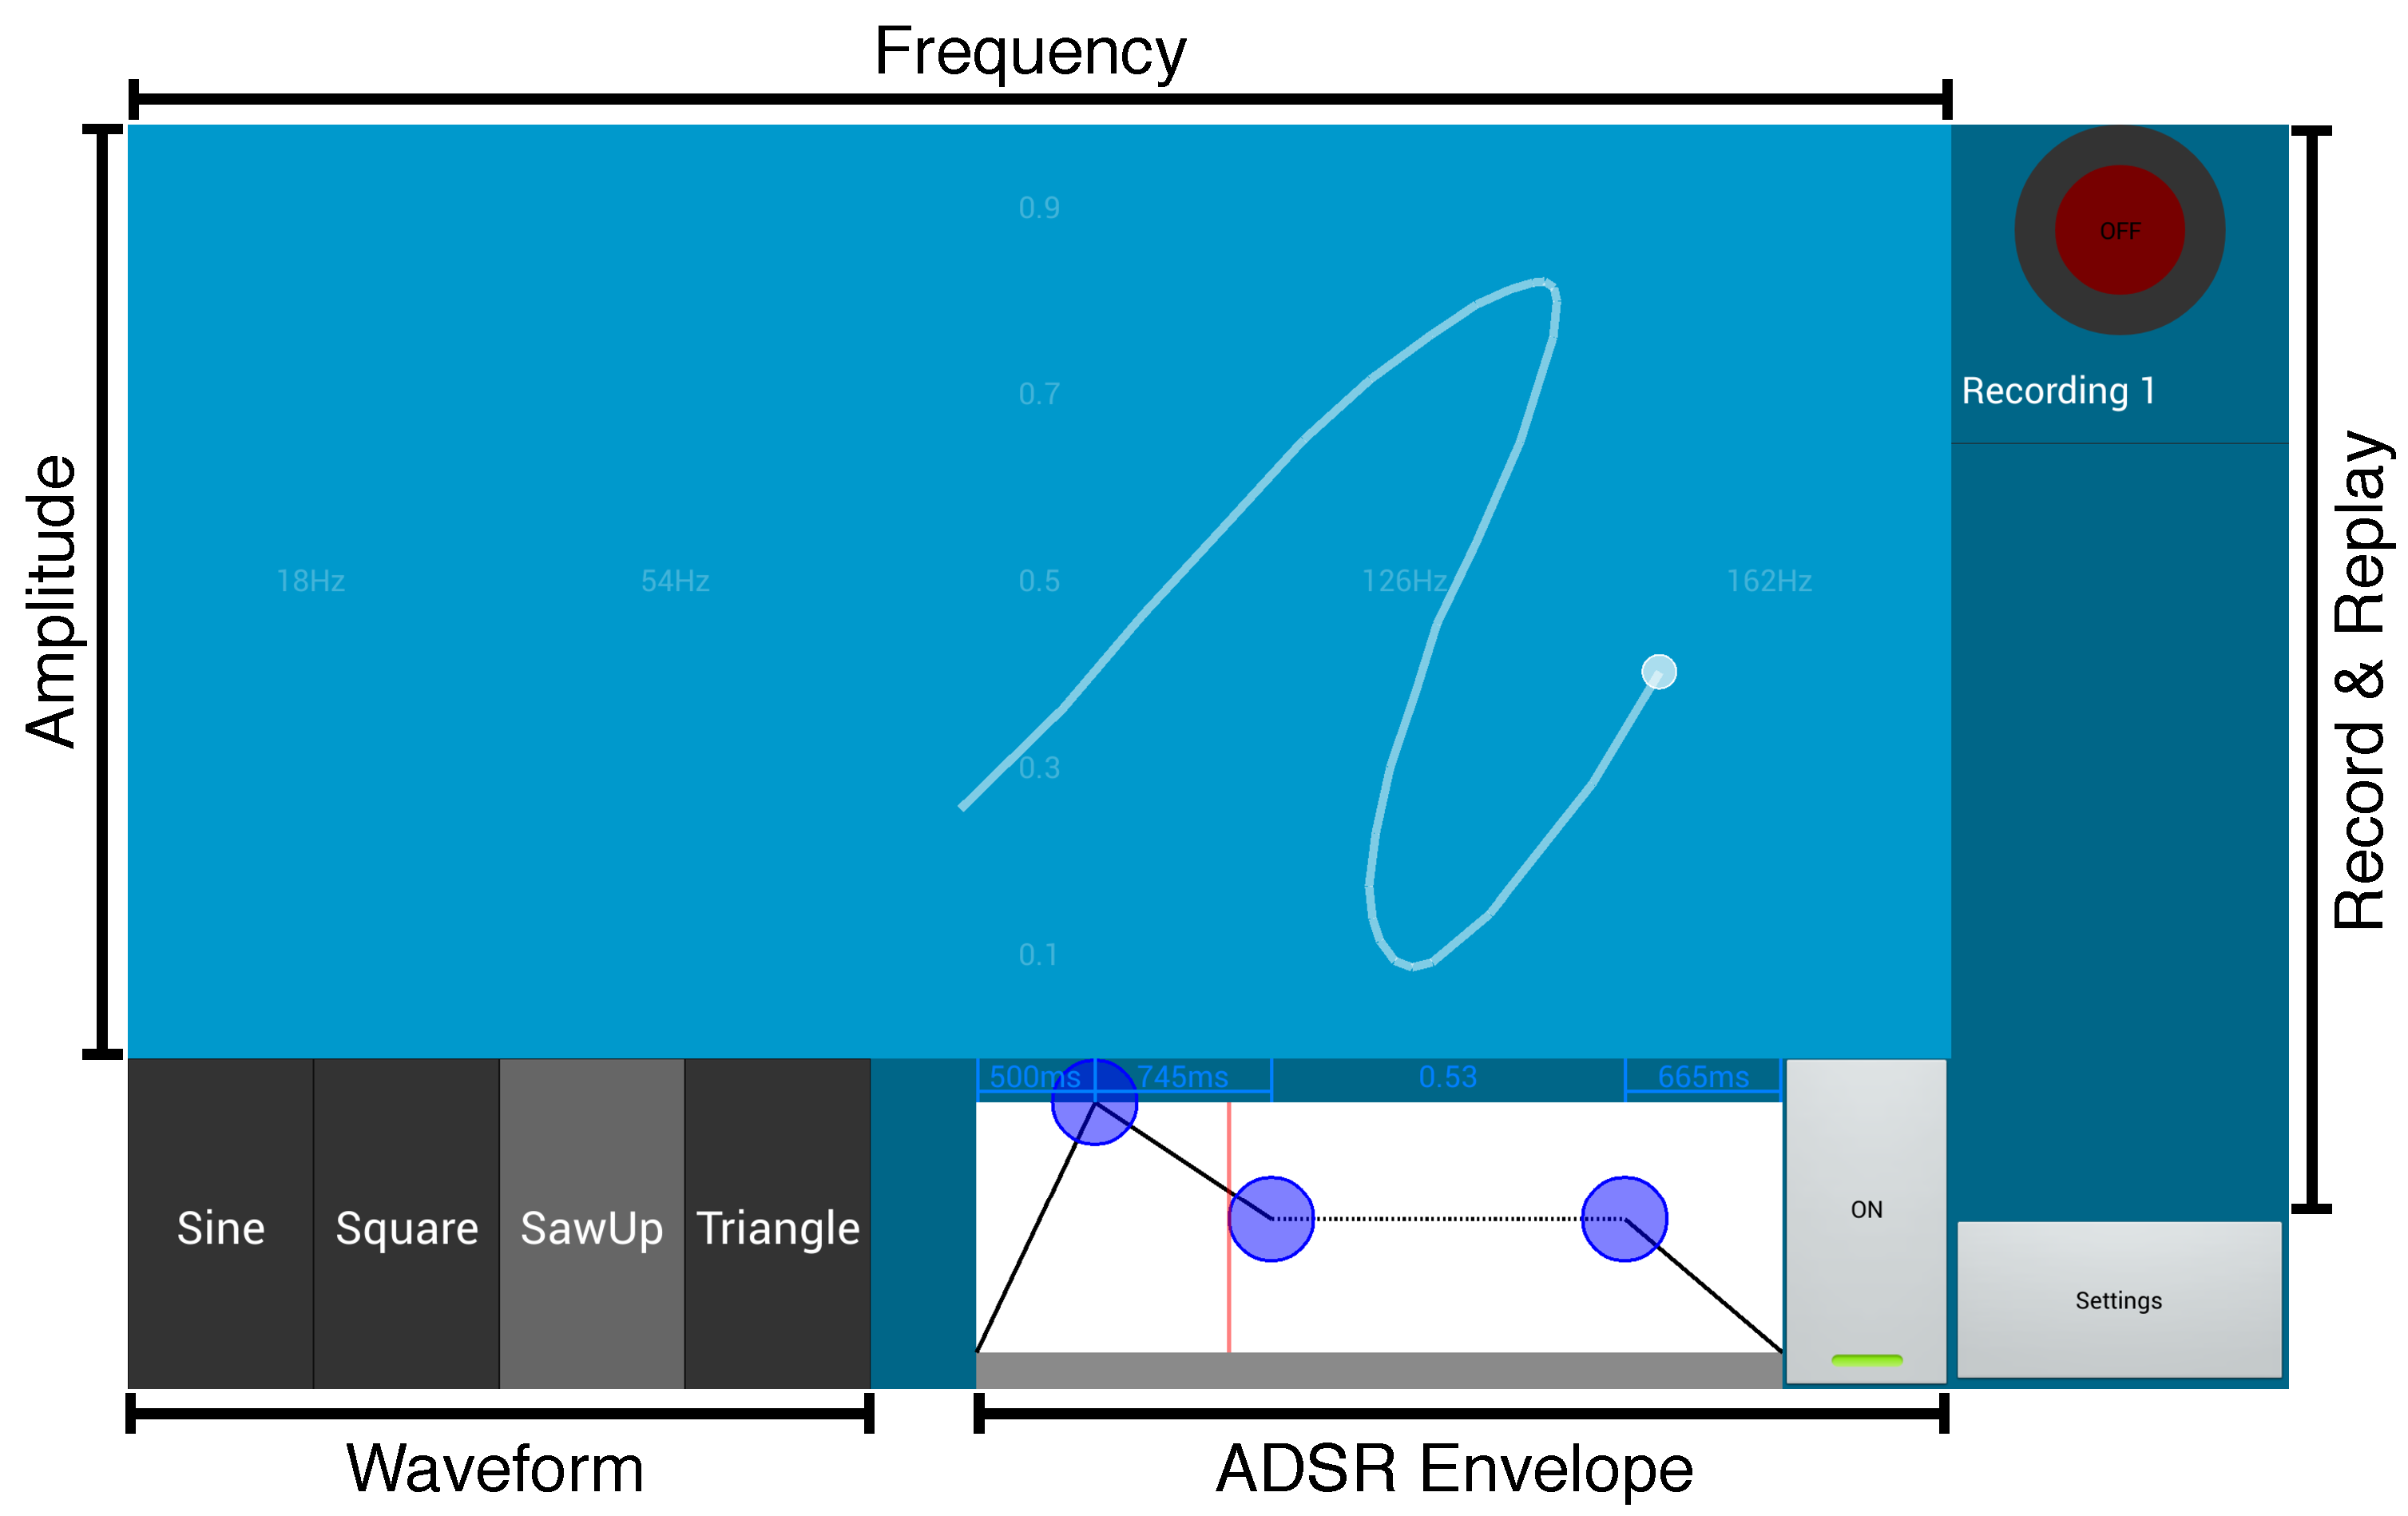
\includegraphics[width=0.43\textwidth]{mHIVE-screenshot-labeled-2013-08-13} 
	   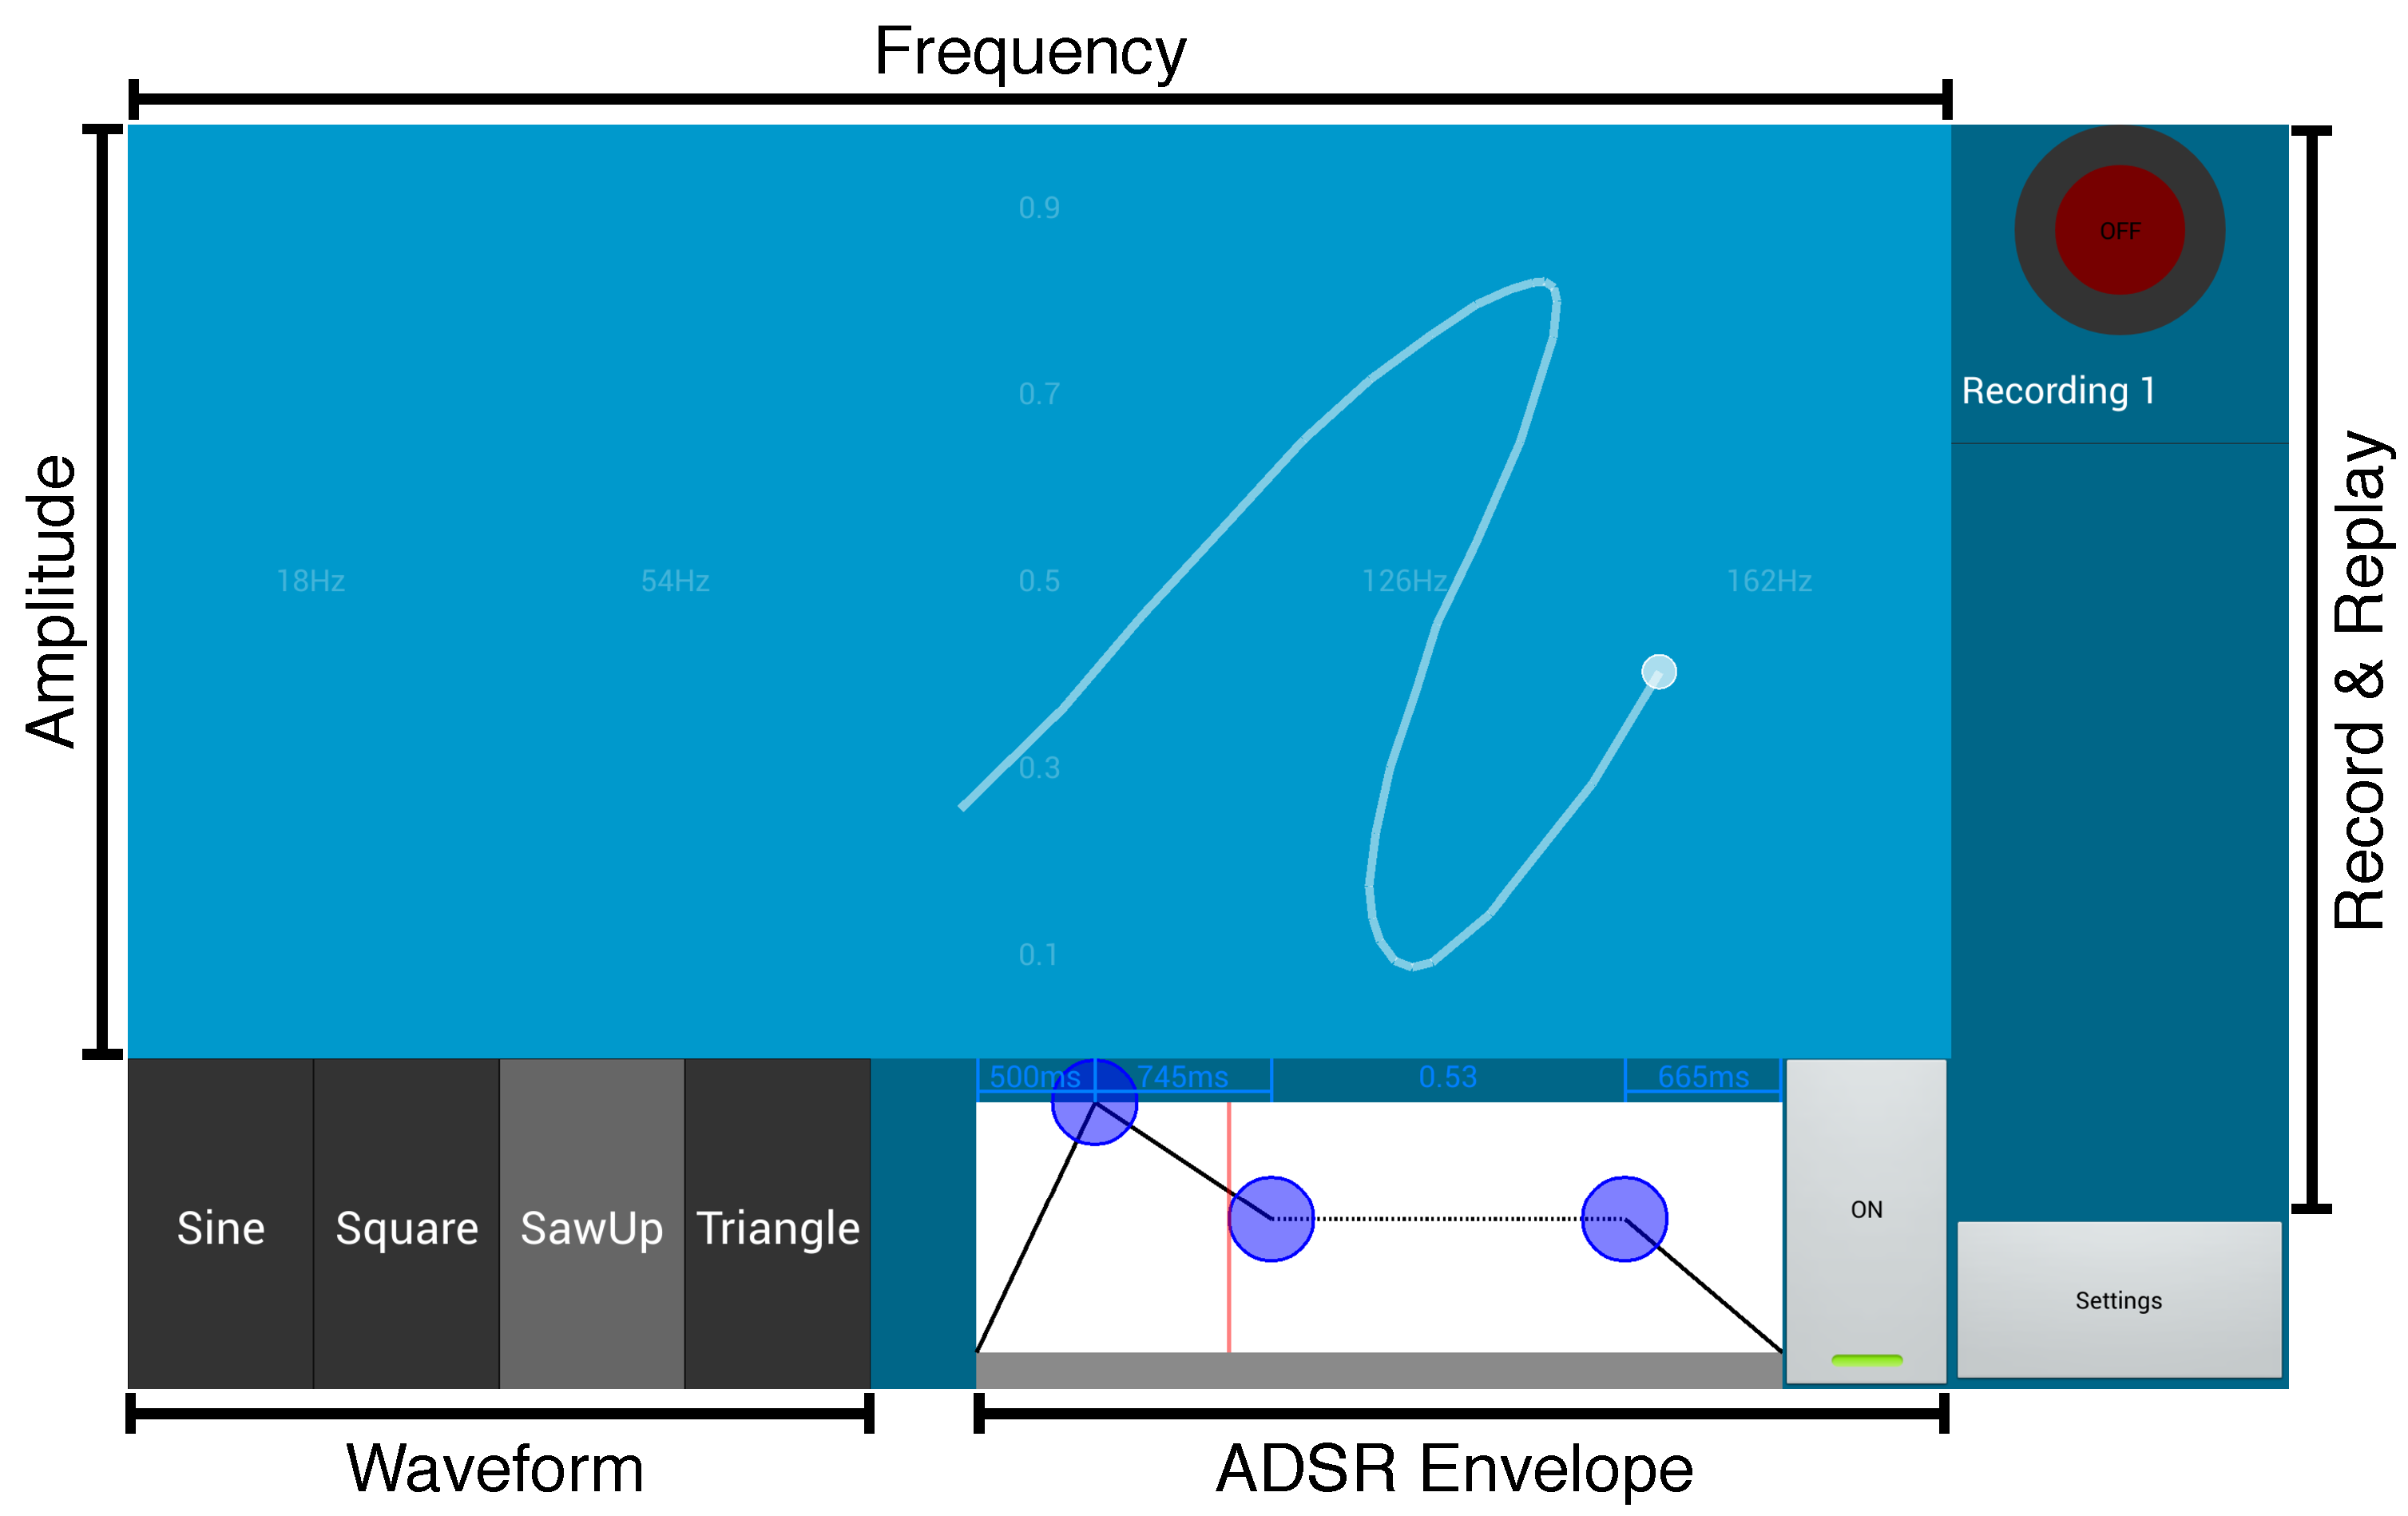
\includegraphics[width=0.7\textwidth]{mHIVE-screenshot-labeled-2013-08-13} 
	   \caption{mHIVE interface. Primary interaction is through the amplitude-frequency view, where visual feedback is provided through a circle (current finger position) and a trail (interaction history).}
	   \label{fig:mHIVE}
    \end{figure}



\subsection{mHIVE}%, a mobile Haptic Instrument for Vibrotactile Exploration}
We developed mHIVE, a mobile Haptic Instrument for Vibrotactile Exploration, to begin to explore how a haptic instrument should work and what it should do (\autoref{fig:mHIVE}).
% , we  developed a prototype, mHIVE (mobile Haptic Instrument for Vibrotactile Exploration,
%
%\footnote{Our first, low-fidelity prototype was named HIVE, before we switched to developing on a mobile platform. }
%
% mHIVE is a collocated, synchronous, mostly private control haptic instrument that controls 2 vibrotactile actuators
mHIVE is a collocated, synchronous haptic instrument for a single user. It accommodates shared display via dual
Haptuators~\cite{Yao2010}
and is operated with a single-touch tablet-based interface for direct manual control (\autoref{fig:hapticinstrument:StudySetup}). 
mHIVE is designed for for VT
% We chose this as a simple first attempt at a haptic instrument: vibrotactile 
sensations, which are common, do not require interactive programming, are controlled through waveforms (analogous to music), and their low-level control parameters are well understood.
%As well, they are commonly used in commercial devices, such as smartphones.
%Using a touchscreen % interface 
%allowed %was chosen for 
%direct manual control, similar to most musical instruments. % of the control parameters.
%: early desktop prototypes were awkward.



mHIVE offers real-time control of frequency, amplitude, waveform, envelope, duration, and rhythm, identified as the most important parameters for VT sensations \cite{Gunther2002,Brown2006a,Brown2006,Brewster2004, Rovan2000}.
mHIVE is implemented in Java using the Android SDK \cite{AndroidOpenSourceProject2012}, and the FMOD sound synthesis library \cite{fmod2013} to produce sounds, sent to two or more Haptuators through an audio jack.
%Thus, mHIVE is effectively a sound synthesizer designed for tactile sensations.
We deployed mHIVE on an Android Nexus 10 tablet running Android 4.2.1.



%mHIVE allows for control of frequency (5-180Hz, determined through piloting) and amplitude (0 (min) to 1 (full)) by drawing on a main input canvas.
%The ADSR filter can be toggled on or off by an adjacent button.
%As well, mHIVE allows for the user to record their input for later play back.
%Recording captures all input events, including waveform selection, ADSR manipulation, frequency/amplitude input, and even recording playback.

%%%%%%%%%%%%%%%%%%
%
% SECTION: Study Methodology
% 
%%%%%%%%%%%%%%%%%%
%\clearpage
\section{Study}

%%%%%%%%%%%%%%%%%%
%
% SECTION: Study Methodology
% 
%%%%%%%%%%%%%%%%%%
%\clearpage
% With mHIVE built, 
We conducted a qualitative study to investigate two questions.
%\km{Q1/Q2?slc} % consider numbering them for more structered reference later. gives a bit of formalism.
First, is mHIVE an effective tool for the expression, exploration, and communication of affective phenomena?
Second, what language, mental models, and metaphors do people use to describe vibrotactile sensations, and how do they relate to mHIVE's low-level control parameters?

\begin{figure}[Htb]
	\centering
%	   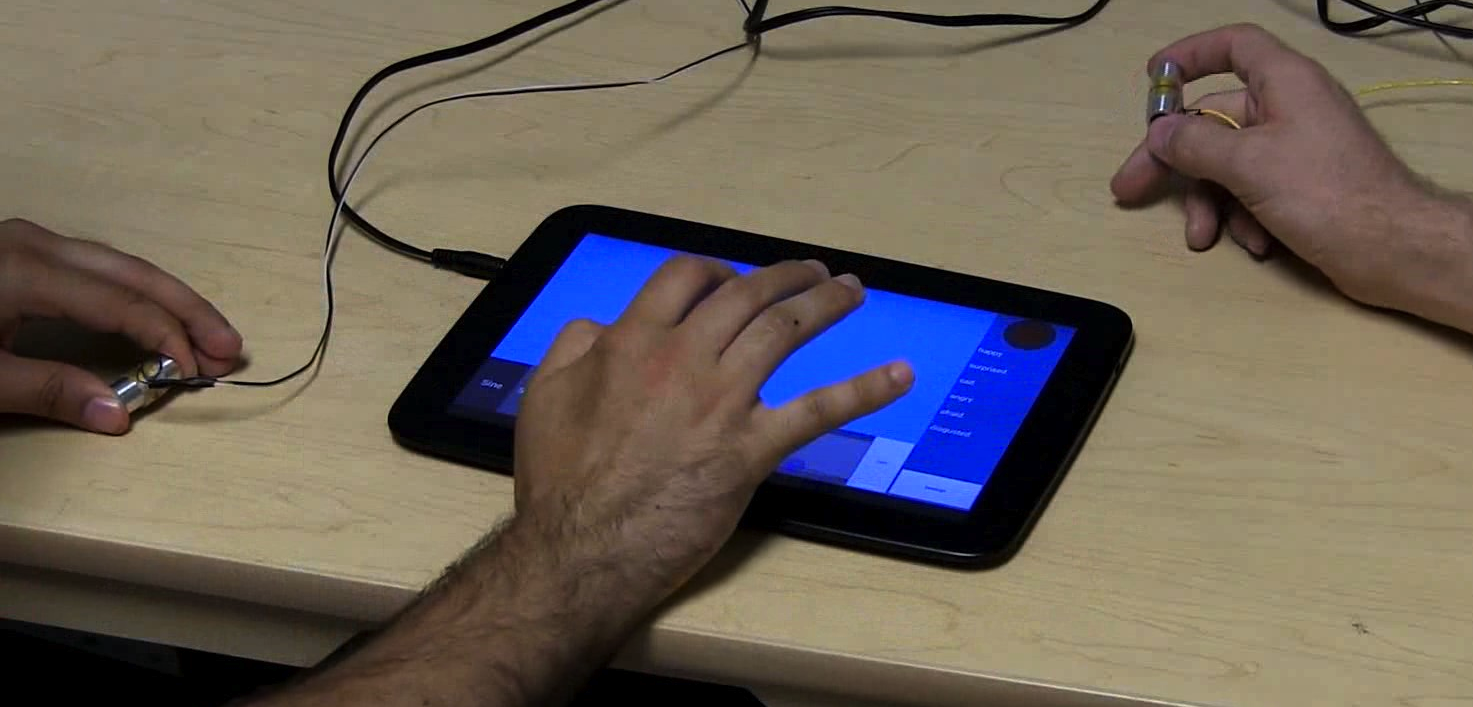
\includegraphics[width=0.32\textwidth]{mHIVE-study-setup-cropped2} 
	   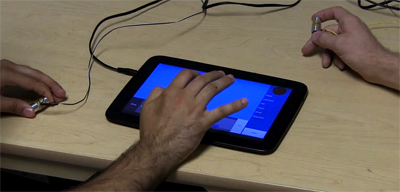
\includegraphics[width= 0.65\textwidth]{mHIVE-study-setup-cropped2small} 
	   \caption{
	   Study setup. Both the participant (left) and the interviewer (right) feel the same sensation as the participant controls mHIVE.
%	   The participant (left) controls mHIVE while feeling the sensation; the interviewer (right) feels the same sensation.
}
	   \label{fig:hapticinstrument:StudySetup}
\end{figure}

%\subsection{Procedure}
One researcher collected and analyzed data using the Stevick-Colaizzi-Keen method as described by Moustakas \cite{Moustakas1994}.
Our 1-hour open-ended interviews
%with four participants, all with haptic experience.
used the following protocol:
\begin{enumerate}
	\item Ask the participant for their background: occupation, experience with touchscreens, haptics, music, and video games.
	\item Demonstrate mHIVE to the user, and invite them to explore while thinking aloud to describe the sensations they feel.
	\item Probe the design space by asking participants to explore different control parameters, and to explore their metaphors (\emph{e.g.}, if the participant describes a sensation as ``smooth", R1 would ask them to try to produce a ``rough" sensation).
	\item Ask the participants to produce sensations for the six basic cross-cultural emotions documented by Ekman \cite{Ekman1992}, and rank how well they think their sensation represents the emotion on a 4-point semantic differential scale (Very Poorly, Somewhat Poorly, Somewhat Well, Well). This was done both as an elicitation device to gather a wider range of interactions with mHIVE, and to directly investigate a design task.
	\item Set the Haptuators down, and ask the participants to describe their experience of working with mHIVE in as complete detail as possible to evaluate the device itself.
\end{enumerate}

\noindent
R1 conducted the interviews and analysis, which required specialized knowledge of mHIVE.
%, and inductive nature of analysis did not allow for other researchers to cluster separately.
% Because clustering was conducted and not coding, 
%\kmEdit{Because we conducted clustering rather than coding,??}
Scores of inter-rater reliability common with other qualitative analyses (\emph{e.g.}, grounded theory \cite{Corbin2008}) are inappropriate and unavailable, as we did not conduct deductive, low-level coding.
To improve reliability,  R1's documented experience was analyzed first, and then consulted during analysis to remove bias (\emph{e.g.}, to not use terms only used by the experimenter).
%documented and analyzed his own experience with the device, which was considered when conducting analysis.
%we present here separately from other results to clearly demarcate the researcher's biases and preconceptions.
%Even so, results are grounded in empirical data, shown by quotations representing the clusters.
%Participants will also be contacted after analysis to provide feedback on our initial conclusions \textbf{TODO}.

%%%%%%%%%%%%%%%%%%
%
% SECTION: Results
% 
%%%%%%%%%%%%%%%%%%
\section{Results}

We sought participants with experience designing haptics as a proxy for expert designers for our initial study.
Four participants were recruited through email lists and word-of-mouth (P1-4, three male), and were all in the age range of 26-35 with self-reported occupations including graduate students or post-docs in information visualization, HCI, and human-robot interaction.
All had experience working with haptic technology, and (because of this requirement) all knew the main researcher in a professional capacity, although only P2 had seen earlier prototypes of the haptic instrument.
The small sample size, typical for phenomenological studies \cite{Creswell2013}, was appropriate for the rich data we wanted.
Data collection ended when we achieved saturation of new results, and had a clear direction for our next iteration.

%determined by saturation of new data: when we stopped encountering new data, we stopped recruiting participants.

%Analysis revealed several themes among the participants, particularly about the device's role in the design process, a tendency towards audio metaphors or concrete example-based metaphors, and a notion of enjoyable sensations vs. non-enjoyable sensations.
%As well, usability concerns are reported, suggesting implications for the design of future haptic instruments.

%
% Subsection: Reflections
%
%\subsection{Researcher Reflections and Experience}

%\emph{Note: This section is written by the researcher who led development of mHIVE and conducted the interviews and analysis.}

%%Researcher eval v1
%%As the principle developer of mHIVE, I have a unique outlook on the device.
%%I entered the study with planned improvements derived from piloting.
%%Deliberate exploration of the device revealed a number of takeaways which I will report here.
%%Some are may be similar to the experience reported by study participants, and some are specific to me.

%%Because I built the device, I understood the underlying mental model, and thus found mHIVE to be \q{very intuitive,} and \q{very helpful.}
%%I \q{enjoyed using it.}
%%I found visual trace and ADSR envelope to be \q{helpful.}
%%In particular, ADSR was very \q{important} to me, and was useful to \q{soften the edges} of the sensations.

%%However, I do not believe that mHIVE is perfect.
%%First, the addition of multitouch is \q{important.}
%%I found it was tricky to \q{juggle both hands}, feeling the output while simultaneously controlling the interface.
%%I have mixed feelings about the recording feature. Though I found it \q{helpful the one time} when developing the surprise sensation, I only used it once and feel that it \q{needs work.}
%%I had originally though that the recording feature needed a stop button, but \q{I didn't used it enough to notice} any lack of such a feature.

%%Finally, I found myself changing waveform and ADSR infrequently; it was \q{easy to leave something in place.}
%%Overall, I felt that mHIVE was \q{an exploratory tool} rather than a tool for \q{refinement.}
%%It would be best suited to exporting icons to \q{another application or another task.}

%%researcher eval v2
%Because I built the app, I understood the underlying system model. Because of this, I enjoyed using it, thought it was helpful, and found it intuitive and easy-to-use. I thought visual trail was very nice and helpful, because I could see where it was, and that ADSR was important, especially for a ringing sensation. I experienced unexpected sensations, calling them weird.

%Of course, because I was using an early prototype, there were still some interface-level refinements I thought were important to make. Some of these became less important as I interacted with the device. I thought that it needed a button to stop replay, but because I only used the record/replay feature once when exploring the device and didn't notice the lack of a stop button, I thought it was fine. Interacting with the device, multitouch emerged as an important feature to try. Overall, I though mHIVE was suited for exploration but not refinement, and thought it might be a good idea to record haptic icons and export them to another application.

%Low frequency sensations stood out to me as oscillating, pushes, thumps or hits (with the square wave), and felt like a watch or subwoofer. I described some low-level sensations with onomatopoeias, including djoo djoo djoo, wub wub wub, tick tick tick tick. ADSR allowed sensations that felt like soft bells, and that made me picture the sound of an ocean swelling. I made frequent analogies to technology: lasers, boat motors revving, and zippers, and could hear higher frequencies, comparing them to mosquitos buzzing or high pitched whines like an plane engine.

%I also used tactile metaphors, tingly, strained, taut, grainy, gritty, and rumbly. Triangle and sine waves became more forceful while square and sawtooth waves became stronger. Higher frequencies were smooth, like a constant ringing, and sometimes aggressive, viscious, on edge, or even painful (on one occasion).

%
% Subsection: Themes
%
%\subsection{Themes}
Here we report the three major themes that emerged during analysis: % possibly: use this spot to help with the expansion on methodology, reinforcing that it was systematic not biased, clearly a concern of the reviewers.}
%
 mHIVE's success as a haptic instrument, mHIVE's limitations that reveal more detail about the haptic design process, and the use of language in the study.

\theme{mHIVE Succeeds as a Haptic Instrument}

%mHIVE achieved its goals of exploration and communication. 
Our results suggest that mHIVE can be effective for exploration of a design space, and communication in the haptic domain. % This section does come across as one-sided. Being critical: the goal of exploration/communication is broad and loose (a low bar?) and many statements could be used in support of it. Can you balance with statements that either countered it (showed where improvement was needed) or establish limits? Most helpful now is that you break it down into sub-themes.
Overall, mHIVE was well received, seen as a novel and promising tool.
\nq{1}{I definitely liked it},
\nq{2}{I think there should be more devices like this for designing haptic icons}.
%\nq{3}{It was fine. I mean I guess at the high level, it's relatively easy -to-use}
%\nq{4}{it's a nice, uh, nice sandbox to play in}


\strongitem{Serendipitous exploration}
Participants reported that mHIVE was best served to explore the design space, generate a number of ideas, and try things out.
Serendipitous discoveries and exclamations of surprise were common.
Participants were able to \nq{2}{accidentally stumble upon something} as they explored the device.
%	\nq{1}{what's that going to be like},
%	\sq{maybe something like this�}
%	\nq{2}{it's not like you know, uh, everything in advance, it's not like you're trying to mimic something, you're trying to put random things together and see what meanings you can extract out of it}
	\sq{I felt I could get a large variety},
	\nq{3}{I could easily play around with the high-level to find out what was neat}.
%	\nq{1}{Ooo, that's kinda cool}.

%In addition, mHIVE let the participants "accidentally stumble upon something" (P2), revealed through expressions of surprise when feeling interesting sensations:


%	\nq{2}{Yeah, you feel like, oh this is interesting}

%	\nq{3}{That's an interesting kind of effect there}

\strongitem{Communication}
mHIVE %was not just a tool for exploration, but also communication as it 
established an additional modality for dialogue.
%Participants referred to sensations as a deictic channel, essentially using the device in a manner analogous to gestures.
The dual outputs created a shared context, demonstrated by deictic phrases: the additional context of the vibrotactile sensation was required to make sense of the statement.
The use of ``that" and ``there", reminiscent of the classic ``Put That There" multimodal interaction demo \cite{Bolt1980} indicate a shared reference point was established from the haptic instrument.
\nq{3}{So there'd be like, (creates a sensation on the device), which is pretty mellow}.

In particular, P4 successfully communicated the sensation of sleepiness to the R1, by asking whether R1 could guess the sensation.
\nq{4}{Can you guess it?} \namedquote{R1}{Sleepy?} \nq{4}{Yeah. Pretty good}.
The dialogue worked as a two way channel, as R1 was able to phrase questions using the device.
%, and communicate the sensation of surprise to P4, or pose a question to P2.
	\nq{2}{It was different} \namedquote{R1}{How was it different?} \nq{2}{You delayed the first part, it felt new}.%, but when you make random moves}

Certain sensations, like a feeling of randomness, could only be felt when another person controlled mHIVE.
	\nq{2}{When someone else does it, I feel better, it's like, you cannot tickle yourself}.


%This was revealed especially when discussing a usability flaw in the device, a lag between touching the device and the output of the sensation:
%	\nq{2}{(taps on the device, demonstrating delay) you feel the delay?}
%In addition, the interviewer was able to phrase questions by using the device:
	
	
%	\theme{ADSR envelope has a learning curve}

%\strongitem{Learning curve}
%Like a musical instrument, mHIVE also has a learning curve.
%This is especially true with the ADSR envelope, which was unfamiliar to most participants.
%P4, a musician who had encountered ADSR envelopes before, was more familiar with the concept, but still felt that he could become more expert with mHIVE.
%Though a learning curve limits who can use the device, it might just mean a different target audience, such as experts rather than novices, or designers rather than end-users.
%%ADSR especially required more expertise than the other features:
%	\nq{1}{This little plot dude down here didn't make sense to me at all at first, once you explained it, it totally it did; I'm still not very confident in my ability to map between this plot and sensations, but I kinda get how it would work},
%	\nq{4}{I think it does require a bit of a learning curve}.
%%\nq{3}{I find this a bit harder just to perceptualize, but by the end I think I was starting to get a sense of how it worked, it took me longer than the other aspects to, clue into.}
%%\nq{4}{So I don't know if most people would take the time to use a tool like this to develop a range of different haptic signals for their phone, but this would be a great tool for a designer to use}
%%We suspect that ADSR would be used more heavily by expert users.
%However, some designers might still not want to use ADSR at all.
%\nq{3}{This attack and release, I find it the third most valuable thing [of four].}

%% P2 and found the control confusing when the sustain was 0 (\q{(sustain $<0$), I can control how long it vibrates}, \q{(sustain 0), it's like it dies, and, seems like, um, I dunno I'm less in control of this one}).

%%P4, with experience in digital music, immediately recognized the ADSR. TODO

\theme{Tweaking through Visualization and Modification}

During analysis, some key directions for future design emerged around visualization and control capabilities.

\strongitem{Inability to tweak}
Though mHIVE supported exploration and collaboration, we found % that mHIVE was not a general design tool on its own.
it was inadequate as a standalone design tool.
Few created sensations were considered to be final.
Many descriptions were hedged % with an ``I dunno," 
and in the design task, few sensations captured the emotional content well.%(\autoref{fig:design:bar:plot})
	\nq{1}{I dunno, maybe that's afraid?},
%	\nq{1}{Not bad\ldots I feel that one could do better}, \sq{My angry is somewhat disgusted}
	\nq{2}{Still felt that you can make them better},
	\nq{3}{To me that's more fuming (laughing) than it is angry}.
%	\nq{4}{I'm sure if I spent more time on this, I think we could play around a bit more with the design space.}
On some occasions, participants were certain about their descriptions.
\nq{1}{Sad, definitely down on the amplitude with sad\ldots oh that's totally sad. Yeah.}.
%, \nq{2}{Yeah. This is afraid.}
This was uncommon, and usually tied to discovering an ideal sensation during the design task.

%\begin{figure}[htbp] %  figure placement: here, top, bottom, or page
%   \centering
%   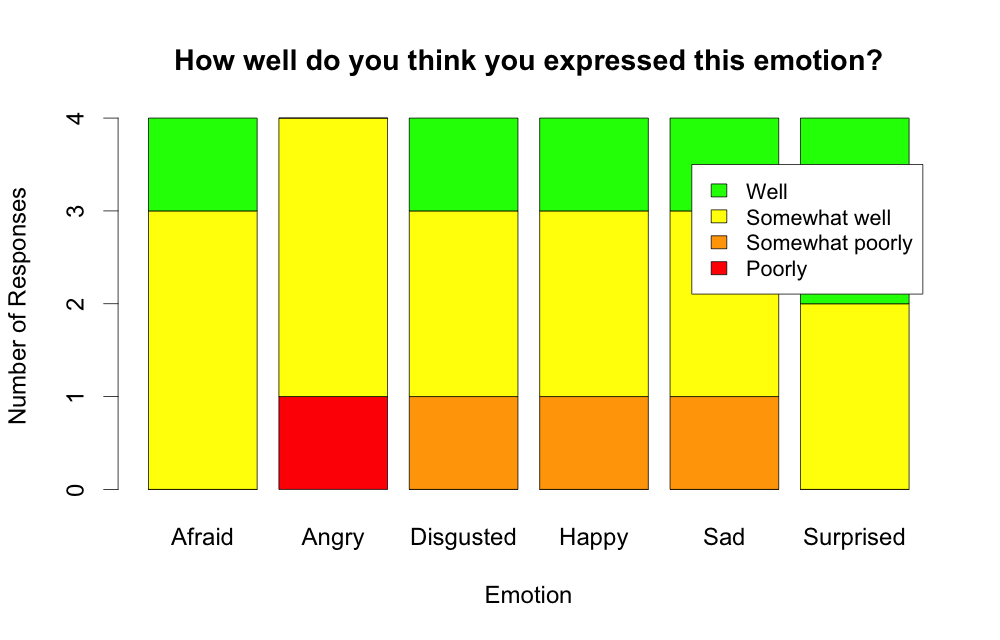
\includegraphics[width=0.47\textwidth]{mHIVE-BarPlot} 
%   \caption{Participant ratings of the confidence in their designs}
%   \label{fig:design:bar:plot}
%\end{figure}


%\strongitem{Memory and attention barriers}
\strongitem{More visualization and recording}
%Though the participants were able to create initial designs for sensations, they were unable to develop them.
Part of mHIVE's inability to support tweaking was due to cognitive limitations for both memory and attention.
Participants found it difficult to remember what they had tried before, % and found it difficult 
and to pay attention to the output % sensation 
while simultaneously controlling it. %the device.
%Participants found significant cognitive challenge in remembering what they had tried before
%	\nq{2}{I tried to recreate that but I couldn't create it exactly as it felt the first time}
\nq{3}{There's a lot of variables which, when I'm trying to compare between two configurations\ldots it was hard sometimes to remember what I had tried},
%if I've done something,
%\theme{Tactile Overshadowing, Looping is required}
%Participants unanimously expressed a desire to feel sensations without having to simultaneously control the device, allowing participants to focus on the sensations they were feeling. This was achieved either by using the recording functionality or the interviewer control mHIVE:
	\nq{1}{I definitely liked being able to feel a stimulus without having to implement it, you know, it allows me to focus more on what it feels like}.
%%	\nq{3}{it's bit hard to do, like I'm trying to go for what I'm imagining, it's hard to do it and feel it at the same time I guess?}
%%	\nq{2}{I tried to recreate that but I couldn't create it exactly as it felt the first time}
%%One thing all participants mentioned was a difficulty remembering what they had previously created or developed. This was partially alleviated by recording, but a desire for more history was deemed important:
%	\nq{3}{It was neat when I could play it back and be like, what did I do and I could see, oh I did that\ldots
%	%and then being able to see where it was was very useful, cuz that helped me in, in what I wanted to be able to kind of replay, like 
%	oh I remember doing something that might work in this situation}.

%This was especially true when the participants noticed a delay between touching the tablet screen and the haptuators activating.  \sq{Feels like there's a delay}, \nq{2}{If I don't look at your finger, I don't see the asynchrony}.

%\strongitem{More visualization and recording}
Participants suggested that although % though 
visualization and recording features helped somewhat %a little 
to overcome these limitations, more was needed. % they needed to be improved.
%All participants requested a further emphasis on recording through repetition or looping.
%This was intended to both aid memory and allow participants to focus on the sensation without worrying about controlling the device.
All  requested greater emphasis on recording through repetition or looping, both to aid memory and allow for focus on the sensation independent of device control. 

%
%\km{SLC***: simultaneous compose/review bad; fluid mode shifting good?} % KM: just struck me: does this undermine the key starting premise that we should be able to perceive the design output AS we create it? In fact, we're finding that this is cognitively too hard. Is it the same for music? Maybe what we have learned is that you need a little space, but not much; and perhaps it is more important that the cognitive effort and time elapsed in moving between composition and review is very streamlined - i.e. you do them separately, but the movement between modes must be extremely fluid.


Allowing persistent, modifiable sensations and alternative visualizations could also help participants overcome these limitations.
%These cognitive challenges were exacerbated when developing more complex sensations.
%mHIVE's recording and visualization capabilities were critical for dealing with these challenges during the design process.
%The visual trail on the main frequency-amplitude screen was especially well received, both aesthetically and for practical use.
%Recorded sensations were important for developing more complicated sensations and augmenting participant memory:
%\nq{2}{The recording functionality I would use for designing more complicated icons that I want to feel different and pleasant}.
%, sometimes goofy or funny
%\nq{2}{Feels great, I love the GUI, a lot},
%\nq{2}{I like the visualization, I like that the history is visible}.
%However, the recording and visualization features are simply not enough as is.
	\nq{3}{The recording records what I do, but it'd be nice to have it repeat stuff},
%This was sometimes meant to mean repeating a single note (P3 quote TODO) but also lead to suggestions of direct manipulation and history:
%Additional visualization was suggested in different forms, improving the trail and seeing the output signal.
%\nq{3}{I almost wanted to be able to see an actual output of the electrical signals\ldots I was having a hard time doing it just by feeling, I would've liked to be able to see it},
%\strongitem{Modification}
%Participants unanimously wanted to modify sensations that had been created.
	\nq{1}{It might conceivably be nice to be able to, you know, draw a curve, draw a pattern, draw like you would in paint, and then be able to manipulate it, replay it, move the points, see what happens}.
%\nq{2}{What I would like to do is, to record something like this, or say go from here to here with the same pace, a constant speed, and then say, okay now, add some acceleration or deceleration to this movement},
%	\nq{3}{Once I zeroed in on something that I thought was close, I almost want to be able to record that spot and then like, tweak it}.

%These design directions may push towards previous tools, like the vibrotactile score \cite{Lee2012, Lee2009}.
%However, it is important to keep some of the novelties created by the haptic instrument, whether as a development paradigm or an interaction technique.
%Rather, combining the two paradigms of editing and collaborative real-time control, either in a single tool or as steps in the design process, might be the best direction. 
%% \kmEdit{slc}
%% Trying to decide if you mean tight integration between two tools in a design-process kind of way; or integrating them within a single tool? 
%	\sq{If you could, transfer this to a desktop computer and then play with it on the desktop computer},
%	\nq{2}{Definitely those options would bloat the interface\ldots so you don't want to sacrifice the good interface that you have for a lot of functionality that a lot of people don't want}.

%One thing all the participants wanted was for recorded sensations to loop and be modifiable:

%	\nq{1}{The other thing was, I think a little bit difficult,is\ldots
%	%you know there was one or two instances where I wanted to, um, you know
%	if I wanted to change something over the course of recording, you know if I wanted to change the waveform as part of the same recording that it was, you know, I couldn't do that quickly}





%%\theme{Visualizations are important}
%%The answer to 
%%Visualizations were critical  \textbf{TODO}
%%The amplitude-frequency view and its graphical trail was well received, especially by P2: \q{Feels great, I love the GUI, a lot}, \q{I like the visualization, I like that the history is visible}.

%P1 enjoyed the visualizations, but wasn't sure if it was useful at first: \q{at first I wasn't sure whether I liked the trails or not, and I still don't think they actually do me any good, but I like them just, aesthetically\ldots you know what maybe they do, because they allow me to, uh, think visually about uh, about what I'm doing and they also allow me to, uh, reproduce and tweak, um, a stimulus.}
%% You know I, I can do this, the output's kind of like that, but I, I, and so the, it's easy to tell I'm doing the same thing again, it's also easy to tell how I'm changing}

%P3 actually wanted more visualization, particularly of the outputted electrical signal: \q{I almost wanted to be able to, um, see like an actual, like, output of the, electrical signals, so that I could really map\ldots I was having a hard time doing it just by feeling, I would've liked to be able to see it.}





%Further comments suggested that the design process was split into two tasks: generation of ideas and tweaking.
%The recording function was a first step towards stronger design capabilities, but tweaking required more power.
%Participants wanted to modify existing stimuli, such as adjusting speed or length of a sensation, automatically loop or sequence sensations, and manually enter values for the parameters (e.g., ADSR).

%%	\nq{1}{but it- it seems like a weird tool cuz it's so constrained, right, but when I think about it as, oh I'm just defining a single tone, um, then it makes sense, and it seems like a handy thing to have.}

%	


%Though participants wanted additional functionality to support tweaking, they thought it might be best implemented in a second tool or mode:
%	
%	\nq{4}{
%	%Either that or if you just have a, selecting, buttons like this, you wouldn't need this free form control, and
%	you'd obviously need two interfaces, one with this freeform, uh digital entry and another one you can just program in what you want.}


%\theme{Hard to remember what was tried}
%Part of mHIVE's inability to support tweaking was due to a poor support of sensation history.


%	\nq{3}{it was neat when I could play it back and be like, what did I do and I could see, oh I did that, and then being able to see where it was was very useful, cuz that helped me in, in what I wanted to be able to kind of replay, like oh I remember doing something that might in this situation.}

%However, the mHIVE's recording and visualization features are not enough.
%Participants were lost in the complexity, and indicated a desire for looping or direct manipulation that would allow changes to existing sensations.
%This is an important direction for improvement, because could help challenges for both attention (by allowing participants to focus entirely on the looping sensation) and memory (by allowing modifications instead of requiring a sensation to be redrawn each time).

%	\nq{1}{it might conceivably be nice to be able to, you know, draw a curve, draw a pattern, draw like you would in paint, and then be able to manipulate it, replay it, move the points, see what happens.}
%	
%	\nq{1}{The other thing was, I think a little bit difficult,is you know there was one or two instances where I wanted to, um, you know if I wanted to change something over the course of recording, you know if I wanted to change the waveform as part of the same recording that it was, you know, I couldn't do that quickly,}

%	\nq{3}{the recording records what I do, but it'd be nice to have it repeat stuff like that}
%	
%These design directions may push towards previous tools, like the vibrotactile score (cite).
%However, it is important to keep some of the novelties created by the haptic instrument, whether as a development paradigm or an interaction technique.
%Rather, combining the two paradigms of editing and collaborative real-time control might be the best direction.

%	\nq{2}{If you could, transfer this to a computer, to a desktop computer and then play with it on the desktop computer},
%	\sq{definitely those options would bloat the, interface so, somehow you want to, um, not go that way, as well, so you don't want to sacrifice the good interface that you have for a lot of functionality that a lot of people don't want.}

%One thing all the participants wanted was for recorded sensations to loop and be modifiable:

%	\nq{1}{The other thing was, I think a little bit difficult,is\ldots
%	%you know there was one or two instances where I wanted to, um, you know
%	if I wanted to change something over the course of recording, you know if I wanted to change the waveform as part of the same recording that it was, you know, I couldn't do that quickly}


\theme{A Difficult Language}
% Unfortunately, We report here on some of the emerging trends.
Our study was too small to analyze language patterns in detail, but exposes emerging trends.

%\theme{ADSR and low-frequencies are pleasant, constant high-frequencies are unpleasant}

\strongitem{Pleasantness, ADSR, and frequency}
Participants often started with a statement of like or dislike rather than a description.
% frequently first stated whether they liked or disliked a sensation, rather than describing  the sensations.
Pleasant sensations often involved the
%Participants used a variety of approaches to describing the sensations that they felt.
%It was sometimes difficult to find appropriate words.
%One of the most common exclamations was whether a participant liked or disliked a sensation.
%This was sometimes more immediate and natural than adjectives.
ramp-in and ramp-out (``echo" or ``ringing") of the ADSR envelope, or lower-frequency sensations.
Longer, higher frequency without ramp-in and ramp-out were less pleasant.
% were especially tied to creating a pleasant sensation.
%In keeping with the literature about touch being connected to affect or \ldots (cite, ask Hasti for refs), participants frequently and readily expressed when they liked a sensation:
	\nq{1}{I don't know how else to describe it, I kinda like it},
%	\nq{3}{I like that}
%This was especially true when introduced to the ADSR envelope:
%	\nq{1}{Oh that's cool, it definitely allows you to change, um, uh, feel, the� niceness? of the tone}, \sq{kinda like that with the square wave, I didn't like the square wave before}	
	\sq{Yeah, this [ADSR] seems natural, somehow}, \nq{2}{It feels unnatural to kill the echo right away},
%	\nq{3}{(TODO)}
%While exploring the device, participants tended to divide frequency and amplitude into two or three discrete values: low, high, and sometimes medium.
%Initially, participants tended to press and hold, rather than tap rhythms (often until prompted by R1).
%The labeled axes divided the main frequency-amplitude interface into quadrants, and afforded this discretization.
%The lower-frequency section (approx. 0-20Hz) provided some variation, when the individual pulses of the actuator could be felt.
%Lower-frequency sensations were often pleasant, while a continuous, high-frequency (150-180Hz) sensation was unpleasant.
%	\nq{2}{I like the sensation of the very low frequency, it's very warm},
	\nq{3}{I like this [low-frequency] sensation cuz to me it feels a lot like purring}.
%Correspondingly, all participants agreed that a sustained high-frequency (right-half of the view, or over 90Hz) was unpleaseant or associated with negative emotions:
%	\nq{1}{I find there's negative emotions I would also associate with high frequencies, definitely anger is a high frequency thing},
%	\nq{2}{I feel like the high frequency one can become disturbing, if the use is prolonged}.
%	\nq{3}{sad was hard, because, I feel like, the high vibration frequencies are agitating so they're okay with negative emotions, and it's a little bit harder at the high speeds to get something that's happier feeling but low, I feel like on this was kind of hard}


%\nq{2}{I'm trying the extreme points first. And middle points.}


\strongitem{Waveform}
%\theme{Waveforms feel qualitatively different, and might gave sensations of frequency}
Participants all noticed differences between waveforms, but were often challenged in expressing them
% although it was often challenging to express the difference
(P4 
%described the differences with 
used the musical term ``timbre").
Square waves in particular were distinct, with a greater range and stronger affinity to mechanical sensations.
	\nq{1}{It's interesting, they feel more different than I thought they would},
	\nq{2}{If you want to make something feel like a motorcycle, you would definitely need square wave}.
%The different waveforms also compounded with frequency -- some waveforms felt like they had higher frequency content in them than others.
%%	\nq{3}{oh not as maybe nice as sine}, \sq{I like it better with the triangle.}
%%The different waveforms felt like they had different frequency content. In some cases this was minor or questioned:
%	\nq{1}{The corners must excite other vibration modes, there's definitely more high frequency information there},
%	\sq{Maybe a sine wave with a frequency of f is equal as a square wave with frequency of 2f}, \nq{2}{Saw feels the highest, then sine, then square and then triangle}.
%	P3 noticed and considered frequency differences between the waveforms, but then decided they weren't salient enough.
%	\nq{3}{I don't think the frequencies are changing, I think it's just the style}.
%%\theme{Common descriptors included sonic, tactile, and abstract-affective metaphors}

\strongitem{Aural/haptic metaphors drawn from previous experience}
For the most part, participants used concrete examples and direct analogies to describe sensations, often drawn from their previous experiences.
One stand-out strategy employed by all participants %to describe sensations 
was % the use of 
onomatopoeias: \nq{1\&4}{beeooo}, \nq{1}{vroom}, \sq{bsheeeooo}, \sq{boom}, \sq{neeeaa}, \nq{2}{mmmMMMmmm}, \sq{pa pa pa pa}, \sq{tum tum tum tum}, \nq{3}{tumba tumba tumba tumba}; \nq{4}{upward arpeggio, like, (singing with hand gestures) na na na naaa}.
Other sound-based metaphors were very common, including hum, buzz, whistle, rumble (P1); bell (P1, P2); squeaky, creak (P2); or thumpy (P3).
%Part of this was influenced, for P1, by hearing the haptuators (especially at higher frequencies).
%In response, R1 reduced the volume for P2-4.
%Audio metaphors were still used; even the word ``sounds" was used instead of ``feels": \nq{4}{Triangle, sounds nicer, er feels nicer (laughing)}.
%This may be isolated to vibrotactile output, and might not generalize to force-feedback output.
Still other descriptors were directly haptic in nature:
rough, flat (P1);
sharp, round, ticklish (P2);
sharp, smooth, cat pawing (P3);
impatient foot tapping (P4).


%\strongitem{Previous experiences}
%Participants especially drew on their previous experience for direct haptic metaphors.
%P3, a pet-owner, used several biological metaphors related to her background:
%	\nq{3}{%As you know, 
%A lot of my experience developing haptic outputs has been trying to develop biological metaphors for haptic outputs, so I think in part, I'm just used to thinking about these kinds of things, the kind of biological, twist to them?}.
%%	 Or more natural twist, um, I think that's most of it}
%Biological metaphors were also used by P2 (\q{This feels like someone throwing up (laughing)} ) and P1 (\q{This to me feels like the device is breathing, kind of like a tactile equivalent to the little light on the front of a MacBook}), but were more isolated.

%
%Cars and motors were another common direct metaphor, particularly at low frequencies.
%%This was also related previous experience: P2 mentioned that he pays a lot of attention to car engines, and drives a manual car.
%This was also related to previous experience: P2 mentioned that he pays a lot of attention to car engines, and drives a manual (stick-shift) car.
%This might explain why it was so commonly mentioned, as a car engine is a common experience.
%	\nq{2}{It feels like, feeling cars passing by, as if you can touch something on the side of the road\ldots like a lamp post that vibrates with cars},
%	\nq{3}{Like a car running},
%	\nq{4}{Sort of a revving sound, like revving an engine}.
	
%\strongitem{Few abstract metaphors}
%Although most descriptors were concrete, some more abstract adjectives were used.
%Abstract terms were typically structural in nature, typically involving the control parameters (amplitude, frequency).
%Other terms were used, some in relation to an overall strength (intense, dainty, has presence), some affective in nature (goofy, serious, playful).
%We did not encounter enough of these terms to notice trends.

%More colourful abstract descriptors were still related to the control parameters (intense, dainty, has strong, has presence), or affective during the design task.


%%%%%%%%%%%%%%%%%%
%
% SECTION: Discussion
% 
%%%%%%%%%%%%%%%%%%
\section{Discussion}
\osC{TODO: modify and link this discussion to other chapters, once they are better established.}
Here we interpret these themes to draw implications for haptic design tools, and compare to research on the language of haptics.
We then reflect upon our methodology and limitations.

%
% Discussion: Design Tools
%
\subsection{Design Tools}

mHIVE was able to achieve the two main goals of a haptic instrument, facilitating both exploration and collaboration.
Participants were clearly able to explore the different low-level parameters, and encountered serendipitous or unexpected sensations through improvisation.
mHIVE created a shared experience that facilitated communication between R1 and the participants.
%The dual outputs created a shared context, demonstrated by deictic phrases where the additional context of the vibrotactile sensation was required to make sense of the statement.
%Direct expression of haptic ideas without names occurred: Participants referred to stimuli as ``this" or ``that," meaning that participants did not need to give names to sensations to discuss them.
%The device was sometimes used as a means of almost gestural expression inserted into conversation.
We can thus conclude that haptic instruments are a promising new tool in a haptic designer's arsenal, with a first, successful implementation in mHIVE.

However, the second theme shows that serendipity and communication are only part of the equation.
mHIVE does not serve as a general editor of haptic sensations.
In particular, participants found their attention split when controlling the device and feeling the sensation; perhaps the real-time control should allow for a rapid, but not instantaneous, switch in focus between control and perception.
%Though mHIVE was successful in its goals, its present form does not also serve as an editor.
More generally, participants were unable to tweak sensations because there was insufficient support for comparing ideas or evolving an existing idea.
%for previous sensations, memory and attention. difficulty of remembering what had been explored before, and the difficulty of paying attention to the sensation perceptually while creating it.

% This difficulty is unsurprising, 
In hindsight, this general difficulty is understandable given the broader context of the musical instrument analogy we used for inspiration.
%The other two problems are cognitive-perceptual barriers that must be addressed when considering the entire work flow for haptic sensations.
Musical instruments are not used to write songs on their own, but % need to be 
combined with notation or recording media.
% This
A similar combination of a haptic instrument and recording might be described more succinctly as %with
 a \emph{haptic sketchpad}.
Sketching is critical in design because it allows for the evolution of an idea through multiple sketches, as well as criticisms, comparisons, and modifications \cite{Cross2011}.
%By adopting a more visual, modifiable tool, we can support tweaking.
Emphasizing a history feature that supports multiple versions of sketches, the user could develop an idea as if with a multiple pages in a sketchbook.
Haptic sketching in hardware has already been shown to be %very 
effective \cite{Moussette2011}.  %; we plan to explore more visual metaphors with future iterations.
As well, a visual metaphor resonates with the desire for more effective visualization.
%, so a software perspective might be promising
%A haptic sketchpad would make heavier use of visual working memory to offset the noted perceptual-cognitive challenges with .
%Of course, effective visualizations are challenging, and are left to future work.

Ultimately, haptic instruments may be most useful as one element
% might be useful as one type of tool  % 
in a suite, or component of a more general tool.
% As part of a suite of tools, mHIVE or other 
A haptic instrument could complement % work together with 
a graphical editing tool that does support tweaking, such as the vibrotactile score \cite{Lee2012,Lee2009} or the hapticon editor \cite{Enriquez2003}.
%This path mirrors musical development directly, and so more inspiration might be from digital audio tools.
As part of a more comprehensive tool, mHIVE could be improved to reduce cognitive barriers to memory and attention.
Alternatively, we could add functionality to mHIVE to support looping, visualization, and direct manipulation of the sensations within the tool.
We will explore these options as we iterate on mHIVE's design in future work.

%This latter approach might suggest that musical instrument metaphor needs to be used more broadly.



%
% Discussion: Language
%
\subsection{Language}

Our preliminary results for language are compatible with the literature,
%providing inductive, empirical evidence
supporting previous work.
% The
Participants' readiness to say whether a sensation was pleasant or not supports the 
% current consensus % KM: I wouldn' say it's a consensus yet.
view that touch is affective in nature, and that knowing what one likes or doesn't like is a primary function of touch \cite{Jansson-Boyd2011}.
ADSR pleasantness and high-frequency unpleasantness are both consistent with the literature: Zheng and Morell note that ramped signals influenced affect more positively than step signals, and 3s high-frequency sensations were annoying or agitating \cite{Zheng2012}.
The heavy use of onomatopoeias is reminiscent of Watanabe \emph{et al}.'s work with static materials \cite{JunjiWatanabeTomohikoHayakawaShigeruMatsuiArisaKanoYuichiroShimizu2012}.
%, albeit in English rather than Japanese.
However, in our study, onomatopoeias were often used to express dynamic sensations (beeeooo being a gradual decrease in amplitude and frequency), which might be a useful direction for future work.

%Participants tended to split the frequency space into either low/high, or low/middle/high frequency regions.
%Though this lends support to the low/high frequency split found in the literature \cite{Obrist2013,Zheng2012}, participants did use dynamic changes in both frequency and amplitude, again suggesting that dynamism is an important direction for future work.

%Because of the consistency with the literature, our other discovered language themes might be appropriate for future areas of research.
%Personal experience and direct analogies might make promising starting points for designers, by focusing on making tactile sensations based on common experiences.
%As the language of touch is developed, we can even consider using higher-level parameters, such as changing the ``roughness" or ``pleasantness" of a sensation, rather than frequency or amplitude.
%This will require more analysis, and is left to future work.
%However, we can say that the parameters chosen for mHIVE seem to be effective for controlling vibrotactile stimuli at this point in time.

%
% Discussion: Methodology and Limitations
%
\subsection{Methodology and Limitations}

Although phenomenology is uncommon in the haptics community (excluding \cite{Obrist2013}), we found it to be an effective way to empirically examine the subjective experience of using mHIVE.
%This was especially true when examining the more nebulous concepts of affect, rather than perceptual thresholds found in psychophysics studies.
Because the community is still developing processes and tasks for haptic design, qualitative studies seem to be an especially appropriate way to tackle these problems.
Once we have further defined haptic design, we can then move to more task-based, experimental methods.
%Of course, these will hopefully be triangulated with controlled, statistically rigorous studies.

Our study was a first round of feedback to inform our next iteration, and has limitations.
%There are limitations to this study that we must mention.
First, our participant pool is (intentionally) small,
%Four participants was sufficient for the rich data we needed at this stage in the design process.
and participants were all collected through our professional network, as people with haptic design experience are rare.
As we continue to tackle the problem of haptic design, we hope to seek out a larger and more diverse pool of participants, and %understand different aspects of the problem through different methods.
%In particular, we hope to
explore more realistic design tasks. %with future work as we iterate upon our tools.



%%%%%%%%%%%%%%%%%%
%
% SECTION: Discussion
% 
%%%%%%%%%%%%%%%%%%
\section{Discussion}
Ultimately,
mHIVE was able to achieve the two main goals of a haptic instrument, facilitating both exploration and collaboration, which showed value in real-time exploration and a shared output context.
mHIVE also had limitations - participants could not edit sensations and found it difficult to keep track of multiple sensations.
This is understandable given the broader context of the musical instrument analogy we used for inspiration.
Musical instruments are not used to write songs on their own, but % need to be 
combined with notation or recording media.
There may be no silver bullet with haptic design tools, with haptic instruments solving a particular set of processes (quick, easy ideation and communication for experts) but not others (final touches, distribution).
Ultimately, haptic instruments may be most useful as one element
% might be useful as one type of tool  % 
in a suite, or component of a more general tool.
%A designer could keep a haptic instrument to quickly sketch ideas while working with a more heavyweight tool that allows for manipulation of a haptic sensation.
%This could be in an ``exploration mode", or perhaps a portable tool to sketch ideas when not near a haptic editing suite.

We follow-up on these leads in our subsequent design studies.
In \autoref{ch:tactileanimation}, we use a persistent model of a VT sensation for an editor, and confirm the value of real-time feedback while expanding the design palette to include spatial haptics.
In \autoref{ch:macaron}, we attempt to mitigate the difficulty of describing haptics and draw upon examples by using a VT design gallery.




%Participants were clearly able to explore the different low-level parameters, and encountered serendipitous or unexpected sensations through improvisation.
%mHIVE created a shared experience that facilitated communication between R1 and the participants.
%We can thus conclude that haptic instruments are a promising new tool in a haptic designer's arsenal, with a first, successful implementation in mHIVE.

%However, the second theme shows that serendipity and communication are only part of the equation.
%mHIVE does not serve as a general editor of haptic sensations.
%In particular, participants found their attention split when controlling the device and feeling the sensation; perhaps the real-time control should allow for a rapid, but not instantaneous, switch in focus between control and perception.
%More generally, participants were unable to tweak sensations because there was insufficient support for comparing ideas or evolving an existing idea.
%
%
%A similar combination of a haptic instrument and recording might be described more succinctly as %with
% a \emph{haptic sketchpad}.
%Sketching is critical in design because it allows for the evolution of an idea through multiple sketches, as well as criticisms, comparisons, and modifications \cite{Cross2011}.
%%By adopting a more visual, modifiable tool, we can support tweaking.
%Emphasizing a history feature that supports multiple versions of sketches, the user could develop an idea as if with a multiple pages in a sketchbook.
%Haptic sketching in hardware has already been shown to be %very 
%effective \cite{Moussette2011}.  %; we plan to explore more visual metaphors with future iterations.
%As well, a visual metaphor resonates with the desire for more effective visualization.
%%, so a software perspective might be promising
%%A haptic sketchpad would make heavier use of visual working memory to offset the noted perceptual-cognitive challenges with .
%%Of course, effective visualizations are challenging, and are left to future work.

%Ultimately, haptic instruments may be most useful as one element
%% might be useful as one type of tool  % 
%in a suite, or component of a more general tool.
%% As part of a suite of tools, mHIVE or other 
%A haptic instrument could complement % work together with 
%a graphical editing tool that does support tweaking, such as the vibrotactile score \cite{Lee2012,Lee2009} or the hapticon editor \cite{Enriquez2003}.
%%This path mirrors musical development directly, and so more inspiration might be from digital audio tools.
%As part of a more comprehensive tool, mHIVE could be improved to reduce cognitive barriers to memory and attention.
%Alternatively, we could add functionality to mHIVE to support looping, visualization, and direct manipulation of the sensations within the tool.
%Many of these results fed into the next case study, Tactile Animation, which expanded to include space and time as controlled dimensions.


\endinput




\newcommand{\qq}[2]{\emph{``#1"} (#2)}
\newcommand{\HAtheme}[2]{\textbf{Theme #1:} \uline{#2}\\}



\chapter{Refine: Tactile Animation}
\label{ch:tactileanimation}

  % \teaser{
\begin{figure}[h]
   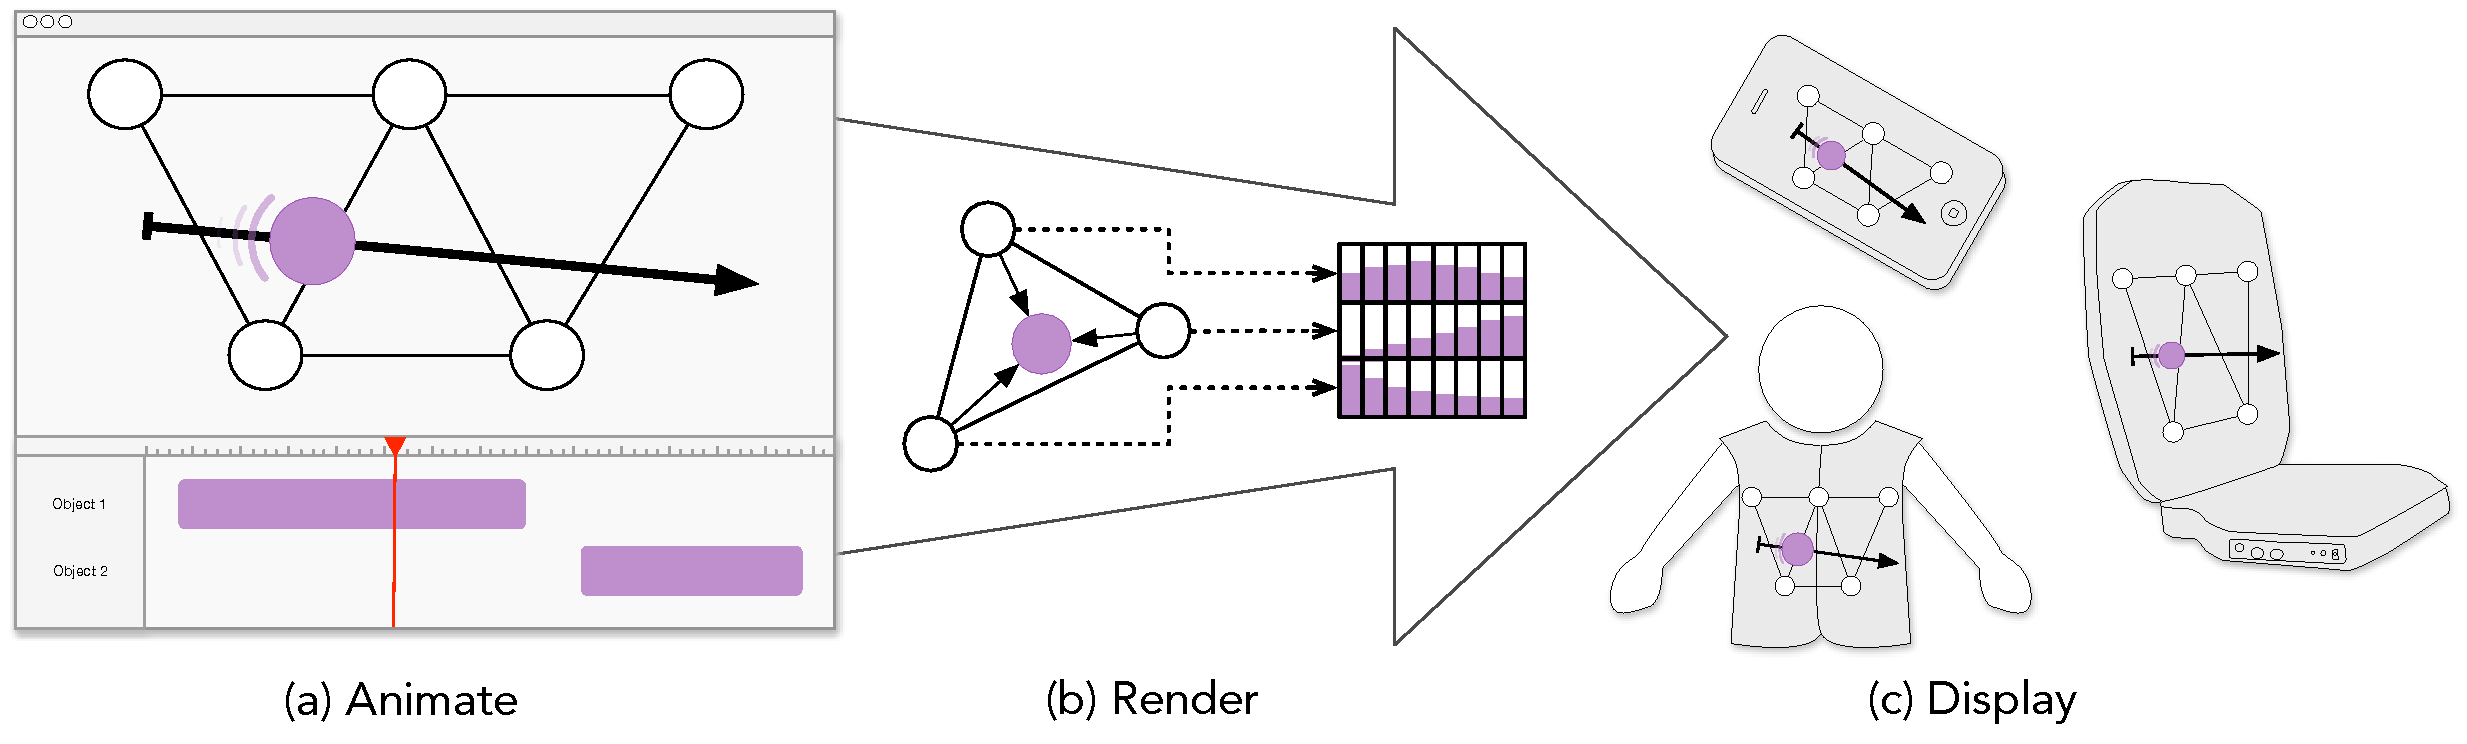
\includegraphics[width=0.98\textwidth]{images/HA14-Concept-Sketch-2015-01-17-1127}
   \caption{Concept sketch for tactile animation. 
An artist draws an animated sequence in the user interface and the user experiences phantom 2D sensations in-between discrete actuator grids. 
%The animator controls phantom sensations directly, without needing to think in device terms, and designs expressive sensations for arbitrary vibrotactile arrays.
}
   \label{fig:concept:sketch}
\end{figure}
% }

  

%Chairs, wearables, and handhelds have become popular sites for spatial tactile display.
%Visual animators, 
%already expert in using time and space to portray motion, could readily transfer their skills to production of rich haptic sensations if given the right tools.
\noindent
\inlineHeading{Preface} In this second case study\footnote{\fullCitation{Schneider2015}}, we iterate on our findings from the haptic instrument to build a full authoring tool that supported both \emph{sketching} and \emph{refinement}.
This work expanded to spatial vibrotactile designs with professional non-haptic media designers.
We surveyed critical haptic authoring tool features and developed a full rendering pipeline for the tactile animation object, an abstraction able to handle diverse spatial vibrotactile arrays. %We describe Mango's interface, rendering pipeline, and perceptually-optimized interpolation algorithm.
We evaluated the implemented tool, Mango, with both phenomenology and methods from grounded theory and iterated on our study tasks.
Professional animators transferred their non-haptic design skills to both explore (sketch) and iterate (refine), but missed features to reuse design elements and gather inspiration from examples.
This theme, also glimpsed in \autoref{ch:hapticinstrument}, lead to the third design activity: \emph{browse}.
%Furthermore, the tactile animation metaphor is a generalizable concept that can extend to several devices.
%, which we explore before concluding.
%in authoring real-time feedback on a variety of grid displays.

%Tactile Animation let us
%\osC{TODO: prosify this additional framing, outline chapter.}
%  - develop a full pipeline editing tool
%  - ground our designs in industry concerns
%  - evaluate with non-haptic media designers to investigate transfer effects
%  - expand our design palette to spatial vibrotactile effects, unexplored directly in the haptic instrument case study
%  - in particular, we expand to a directly-manipulated metaphor
%  - look at device generality in a different way than the haptic instrument. In the haptic instrument, one can build a haptic instrument for new output devices by connecting nput parameters to different output devices. Here we look at a class of devices - 2D vibrotactile grids, but possibly other 2D grids.
%   - this direct manipulation metaphor is distinguished from other spatial control by \autoref{fig:tactileanimation:prevwork}.



\section{Abstract}
Chairs, wearables, and handhelds have become popular sites for spatial tactile display.
Visual animators, 
already expert in using time and space to portray motion, could readily transfer their skills to produce rich haptic sensations if given the right tools.
%We introduce the \emph{tactile animation object}, an abstracted primitive 
We introduce the \emph{tactile animation object}, a directly manipulated phantom tactile sensation.
This abstraction has two key benefits: 1) efficient, creative, iterative control of spatiotemporal sensations,
and 2) the potential to support a variety of tactile grids, including sparse displays.
%enabling direct manipulation of phantom vibrotactile sensations continuously in space and time, and
We present Mango, an editing tool for animators, including its rendering pipeline and perceptually-optimized interpolation algorithm for sparse vibrotactile grids.
In our evaluation,
professional animators found it easy to create a variety of
vibrotactile patterns, with both experts and novices preferring the tactile animation object over
controlling actuators individually.

  
%%%%%%%%%%%%%%
%
% Section - Intro
%
%%%%%%%%%%%%%%
\section{Introduction}

Haptic feedback is
viewed today %in today's
%entertainment and media industry
as a key ingredient of immersive media experiences.
Body-moving devices in theatre seats, ride vehicles, and gaming platforms can tilt, translate, and shake the user for increased engagement. 
Recently, arrays of multiple actuators have been developed to display expressive, spatial sensations on the skin 
%aim to supplement movies, games, and social activities with expressive, synchronized cues at multiple locations 
\cite{Israr2011,Danieau2012a,Sodhi2013,Kim2009,Wilson2014}. 
%Similar opportunities await well-designed wearable and handheld displays.

Vibrotactile (VT) arrays,
which stimulate the skin through vibration, are common in diverse applications from immersive gaming chairs  \cite{Israr2011} to wearable vests for mobile awareness \cite{Jones2004}.
%To create expressive sensations, however, designers typically must be programmers and haptic experts.
%Several device-specific tools for prototyping or final authoring of haptic sensations have introduced user-friendly and user-familiar interfaces.
These displays typically employ sparse actuator arrangements to reduce cost and power requirements, using perceptual illusions to create continuous sensations \cite{Alles1970,Israr2011a,Seo2013}.
Unfortunately, adoption of VT arrays is limited by a lack of authoring tools.
Most only support a single actuator \cite{Enriquez2003}; those that accommodate multiple actuators % deleted Lee2009
control each separately \cite{Kim2009,Paneels2013,Swindells2014},
%Separate actuator control %allow designers to edit, test, and save time-series data for individual actuators, but
%supports smaller, denser arrays \cite{Kim2009} but
%can be 
cumbersome for non-adjacent actuators.
%, with as many as % greater than 
%%10 or 20 vibrating actuators (e.g., one haptic jacket for movie goers is equipped with 
%64 vibrators \cite{Jones2009}.
%%). %(Tactile 

To remedy this, we propose the \textit{tactile animation object}, an abstract, directly manipulable representation of a phantom sensation perceived in-between physical actuators.
% to support real-time spatiotemporal tactile feedback in sparse actuator arrays, enabling direct manipulation.
%{\it Direct manipulation} of a spatial animation object provides
%rather than by coordinating multiple tracks. 
With this approach, designers can 
%eases the transition of visual animators into haptic design.
efficiently and creatively explore ideas and iterate without worrying about underlying actuator arrangements.
As long as a rendering algorithm can be developed, this abstraction not only facilitates design, but is compatible with a variety of form factors and technologies.

In this paper, we describe the tactile animation object and implement it in \emph{Mango}, a tactile animation tool and pipeline (\autoref{fig:concept:sketch}).
Our contributions are: 
%We have three contributions.
1)  A tactile animation interface grounded in user interviews and prior literature.
% The design is derived from interviews and prior literature, ..  includes tools 
%Derived from interviews and prior literature, its design integrates techniques familiar to a mainstream animator workforce. 
2) A rendering pipeline translating tactile animation objects %designed % animated 
%haptic patterns to sparse VT arrays, and optimize its rendering algorithm with a user study.
to phantom sensations on sparse, generalized VT arrays, optimized with a perceptual study.
% We conduct a study to determine an optimal rendering algorithm for sparse VT arrays. 
3) An evaluation with professional animators showing accessibility and expressivity.
4) An exploration of  potential applications for tactile animation.
% with \kmC{SLC} % in  ??? 
%natural user gestures.
% KM 04.12: at this point, 'animation metaphor' as connected to 'natural user gestures' is unclear - you haven't mentioned gestures yet so this comes out of nowhere. Can you restate this contribution more plainly?

%%%%%%%%%%%%%%
%
% Section - Related Work
%
%%%%%%%%%%%%%%
\section{Background}

%%%%%%%%%%%%%%
%
% Subsection - VT perception
%
%\subsection{Haptic Icons and Vibrotactile Perception}

\subsection{Haptic Entertainment Technologies}
Haptic feedback was % has been 
used in cinema as early as \emph{Percepto}, a 1959 multisensory experience for the movie ``The Tingler"  \cite{IJsselsteijn2003} %
%G. Riva, F. Davide, and W.A. IJsselsteijn, �Presence in the Past: What Can We Learn from Media History?,� Being There: Concept, Effects and Measurements of User Presence in Synthetic Environments, IOS Press, 2003, Amsterdam, The Netherlands, pp. 17-40.
with theater seats % The theater seats were 
% equipped with vibrating devices 
that buzzed the audience at strategic moments. % during events in the movie.
Current 4D theaters, rides, shows, and gaming arcades are equipped with sophisticated motion platforms (e.g., D-Box, www.d-box.com) that supplement visual scenes. % with subtle and synchronized movements.
Large tactile transducers (such as Buttkickers, www.thebuttkicker.com) that shake the entire seat using the sound stream are also common with gaming and music content. %, therefore allowing users to feel `bumps' during musical beats and gameplay.   
Custom editors (such as D-Box Motion Code Editor) and software plugins %enable media designers that
overlay visual and audio content with haptics, and allow designers to generate, tune and save frame-by-frame haptics in an allocated track. %for simultaneously with  media content. 

In contrast to displacing the entire body, multichannel haptic devices create percepts of dynamic and localized haptic sensations on the user's skin \cite{Israr2011} and in mid-air \cite{Wilson2014}.
% and in the mid-air \cite{Wilson2014}.
Similar devices have been % are also
developed for online social interactions using custom multi-actuator displays  %haptic devices 
\cite{Kim2009,Tsetserukou2009,Paneels2013}. %Tsetserukou, D. and Neviarouskaya, A. iFeel_IM!: augmenting emotions during online communication. Comp. Graphics & Applications 30 (2009), IEEE, 72-80.
%  Designers (and researchers) for these technologies must have 
% Use of
All of these technologies require extensive programming experience, knowledge of hardware and background in haptic sciences to generate expressive and meaningful haptic content. 
% Due to the lack of
Without guiding principles or haptic libraries,  content generation schemes are complex, device-specific, and time consuming. 


Another class of haptic technology renders high-resolution spatio-temporal patterns on the skin using a sparse array of VT actuators.
These technologies use parametric models of sensory illusions in touch, such as phantom tactile sensations \cite{Alles1970}, and create illusory vibrations in between two or more VT actuators.
%For example, Seo and Choi % KM: when you give authors names in text this way, you can reduce the citation to just the year to avoid clumsy redundancy. However, while I thought there was an easily accessed bibtex citation alternative, I can't find it now. (seem to have to install natbib package and this creates other problems).
%OS: Couldn't figure this one out (biblatex is another package that causes other issues), restructured to be a little less jarring.
%
This idea has been used to % has been done to
create a perceived motion flow between two vibrators mounted on the ends of a handheld device % by controlling their intensity
\cite{Seo2013} and to
%Lee and colleagues
create across-the-body and out-of-the-body illusions on a mobile device using up to four % inexpensive 
%linear resonant 
actuators \cite{Lee2012a}.
The Tactile Brush algorithm \cite{Israr2011a} combined phantom tactile sensations and apparent tactile motion to render high-resolution and moving haptic patterns on the back using a coarse grid of VT actuators, but paths must be pre-determined (\autoref{fig:prevwork:tactilebrush}). 
Other spatio-temporal VT illusions such as the  ``cutaneous rabbit"  \cite{Tan2009} and Tau and Kappa effects \cite{Hayward2008} can be also used with VT arrays.


%Spatial displays of tactors (VT actuators) are a promising avenue for chair-based immersive gaming experiences \cite{Israr2011}, sleeves for social touch \cite{Huisman2013}, or wearable vests for mobile awareness \cite{Jones2004, Brewster2010}.%and artistic compositions \cite{Gunther2002}. Here we cover relevant work on VT communication and perception, and the literature on haptic authoring tools.

%%%%%%%%%%%%%%
%
% Subsection - Haptic authoring tools
%
\subsection{Haptic Authoring Tools}
As long as designers have considered haptic effects for entertainment media, they have needed compositional tools % to facilitate their design 
\cite{Gunther2002}.
% Much previous work has focused on how to prototype, sketch or control haptic phenomena using non-programming methods, % This section highlights those past literature and the 
Requirements drawn from previous work on how to prototype, sketch, or control haptic phenomena using non-programming methods are summarized in
% Key features of these tools are summarized in 
\autoref{tab:design:literature:requirements}.
%A thorough review of prior literature is presented below.

The Hapticon editor \cite{Enriquez2003}, Haptic Icon Prototyper \cite{Swindells2006}, posVibEditor \cite{Ryu2008}, and Immersion's Haptic Studio (www.immersion.com) use graphical representations to edit either waveforms or profiles of dynamic parameters (such as frequency or torque) over time.
%Features include the combination or multi-tracking of effects, utilizing a library of existing effects, and the ability to play back sensations.
Another %popular trend has been to augment  media content with 
approach is predefining a library of haptic patterns to augment media content. %during the development process.
Immersion Corporation's Touch Effects Studio lets users enhance a video from a  library of tactile icons supplied on a mobile platform.
Vivitouch Studio \cite{Swindells2014} allows for haptic prototyping of different effects alongside video (screen captures from video games) and audio. 
These tools focus on low-level control of device features rather than a semantic space, and control devices with either a spatial or temporal component, but not both simultaneously. 




\newcommand\prevWorkWidth{1.25in}
\newcommand\prevWorkImageWidth{1.1in}


\begin{figure}[t]
 \centering
   \begin{subfigure}[t]{\prevWorkWidth}
	  \centering
	   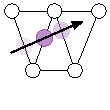
\includegraphics[width=\prevWorkImageWidth]{HA14-PreviousWork-TactileBrush-2015-04-12-1100} 
	   \caption{Tactile Brush \cite{Israr2011a}: precomputed paths}
	   \label{fig:prevwork:tactilebrush}
    \end{subfigure}
    \qquad
  \begin{subfigure}[t]{\prevWorkWidth}
  	\centering
	   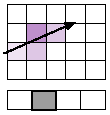
\includegraphics[width=\prevWorkImageWidth]{HA14-PreviousWork-TactileMovies-2015-04-12-1100} 
	   \caption{Tactile Video \cite{Kim2009}: frames of tactile pixels}
	   \label{fig:prevwork:tactilemovies}
    \end{subfigure}
	\qquad
      \begin{subfigure}[t]{\prevWorkWidth}
	      \centering
	   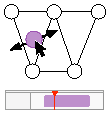
\includegraphics[width=\prevWorkImageWidth]{HA14-PreviousWork-HA-2015-04-12-1100} 
	   \caption{Tactile Animation: direct manipulation}
	   \label{fig:prevwork:ha}
    \end{subfigure}
    \caption{Comparison between related systems.}
    \label{fig:tactileanimation:prevwork}
\end{figure}




\begin{table*}
	\begin{tabular}{|l|p{0.92\textwidth}|}
	\hline
	\rowcolor{tableheadercolor}

	\textbf{LR}
		%& \textbf{RW}
		& \textbf{Description} \\
	\hline
		LR1 
		 &
		 \textbf{Real-Time Playback} \cite{Moussette2011,Schneider2014}
		 Rapid prototyping is essential for working with VT sensations, especially in absence of objective metrics. % of success.
		 Feeling a sensation at design time allows iteration to converge faster to better results. % and develop more engaging sensations.
		 However, \textit{too} real-time can cause split attention.
	\\
	\hline
		LR2 & 
		 \textbf{Load, save, manipulate}
		 \cite{Resnick2008,Johnson2002,Schneider2014}
		 	A persistent object model is essential for sensation editing over % for being able to continue to work on sensations for 
			longer projects and % for being able to share them 
			sharing with other designers or across devices.
			Well-defined actions upon a data structure also facilitates features like \textit{undo} that support experimentation.
	\\
	\hline
		LR3 &
		\textbf{Library of effects} \cite{Enriquez2003,Swindells2006,Herring2009,Paneels2013,Swindells2014}
		% deleted Paneels2010
			 A library of saved sensations is an important feature used in previous haptic authoring tools, providing inspiration and preventing designers from re-inventing the wheel.
	\\
	\hline
		LR4 &
		\textbf{Device configuration} \cite{Kim2009,Paneels2013,Lee2012,Lee2013}% deleted Lee2009
			~Because of the many types of haptic devices, a general tool must be able to understand different devices.
			Lightweight configuration files are common in the literature, allowing users to select specific hardware, specify location and type of actuators, and choose a rendering algorithm.
%			Animators can also select a rendering algorithm from a list of available ones.
	\\
	\hline
		LR5 &
		\textbf{Multiple channels \& combination of effects}
		 \cite{Enriquez2003,Swindells2006,Ryu2008,Paneels2013,Swindells2014}	 
		 Being able to display multiple effects simultaneously, or combine effects via superposition or concatenation, is essential for expanding the design space.
		 This is typically represented in a timeline, which represents the temporal behaviour of any objects.
	\\
	\hline
		LR6 &
		\textbf{Visual/direct control metaphor}
		\cite{Kim2009,Paneels2013,Cuartielles2012}
		 Most previous tools consider each actuator separately.
		 When thinking semantically about a spatial system, a direct view of the device and actuator layout is critical for direct manipulation.
	\\
	\hline
		LR7 &
		\textbf{Audio/visual context}
		\cite{Kim2009,Swindells2014,Moussette2011}
		 Haptic perception depends greatly on additional senses \cite{Hayward2008}. %cite hayward or pseudohaptics
		By providing audio and visual feedback, these effects can be mitigated and the designer can experience haptic sensations in context.
	\\
	\hline
		LR8 &
		\textbf{User Feedback}
		 \cite{Schneider2014,Swindells2014}
		 Receiving feedback from users, either by demonstration or A/B testing, is extremely valuable.
	\\
	

	\hline
	\end{tabular}
	\caption{Literature Requirements (LRs) for a tactile animation authoring.}
	\label{tab:design:literature:requirements}
\end{table*}


Several tools have allowed users to author haptic content using accessible touchscreen interactions.
A demonstration-based editor \cite{Hong2013} allowed control of frequency and intensity by moving graphical objects on a screen.
mHIVE \cite{Schneider2014} controls frequency, intensity, waveform and envelope of two tactors with touchscreen gestures.
Both systems were shown to be intuitive and easy to use for exploration or communication, but faltered when refining more elaborate sensations. % for a set context. 
Commercially, Apple's vibration editor (since iOS 5, 2011)  allows users to create personalized vibratory patterns by touching the screen, but only produces binary on/off timing information.


Other aids to creating haptic phenomena include haptic sketching \cite{Moussette2011} for hands-on exploration of haptic ideas in early design, and end-user customization of tactile sensations \cite{Seifi2014}.
Both emphasize exploration and broad manipulation rather than finely controlled end results.
HAMLAT \cite{Ferre2008} supports authoring of force feedback in static 3D scenes. 
Lee and colleagues \cite{Lee2012} used a musical metaphor for vibrotactile authoring.
Schneider et al. introduced ``FeelCraft" for end user customization of
%to create expressive haptic content using 
a library of \emph{feel effects} \cite{SchneiderAsiaHaptics2014}.
%By tuning parameters of these effects, users could personalize  haptic content, embed it in games and share effects with other users.

Kim and colleagues offered combined spatial and temporal control using a tactile video metaphor for dense, regular arrays of tactile pixels (``taxels"), including a feature of sketching a path on video frames \cite{Kim2009} (\autoref{fig:prevwork:tactilemovies}).
While a promising approach, this tool relies on editing of discrete actuators and frames, with its sketching feature used for input, not as a manipulation method.
As well, it does not generalize to sparse or irregular displays, and was not evaluated with designers.
We suggest that an animation metaphor could provide an easier interaction model, facilitating key creative activities such as rapid exploration and iteration, especially through a continuous timeline (\autoref{fig:prevwork:ha}).
%Further, an animation metaphor could generalize to
%Further, interpolating between actuators works for
%sparse, irregular displays appropriate for larger areas (\autoref{fig:prevwork:ha}).
The control of multi-actuator outputs has also been explored by TactiPEd \cite{Paneels2013} and Cuartielles' proposed editor \cite{Cuartielles2012}.
However, these approaches still require the separate control of different actuators, rather than a single perceived sensation produced by the multi-actuator device. 





%%%%%%%%%%%%%%
%
% Section - Requirements Gathering
%
%%%%%%%%%%%%%%
\section{Tactile Animation Authoring Tool}
% The objective of the haptic authoring tool 
Our objective is to provide media designers with a familiar and efficient % authoring
framework for creating dynamic haptic content. Mango's design is based on two sets of requirements: Literature  (``LRs", \autoref{tab:design:literature:requirements}), from prior research on haptic authoring tools, and Industry (``IRs") from interviews with five industry experts in haptic media creation and animation, which confirm and expand upon design decisions for other VT tools.

\subsection{Gathering Design Requirements}
We interviewed two industry experts with haptics experience from a media company (E1-2).
E1 % has experience with haptic technologies and % KM 04.12: redundant with previous statement
uses Max/MSP, OpenFrameworks, Processing, and Visual Studio to create haptic media.
E2 is a professional media designer and an expert user of Pro Tools (an industry standard for authoring sound media).  Together, E1 and E2 previously undertook 
a six-month training that included generation of dynamic haptic experiences on seats and supporting platforms using audio and video tools.
Our interviews included meetings, recordings, and sketches of their experience during training.

In addition, we conducted contextual interviews of three industry animators (A1-3) interacting with non-tactile animation tools using a think-aloud protocol.
A1 and A3 used Adobe After Effects, while A2 used Maya.
A1 and A2 were tasked with creating an animation of two balls moving; A3 created an animation based on a sound file.
These interviews yielded rich detail that we %and useful information that was 
 compiled into % a small set of 
 categories, then compared with our LRs % presented in 
(\autoref{tab:design:literature:requirements}). LRs 2-7 also emerged independently from this stage.
% these interviews and observations.
We extend the LRs with additional expert-drawn {\bf industry requirements (IRs):} % KM 04.12: definition of IR was too buried, so added bf 

\emph{IR1 - Animation window} allows users to draw tactile animation objects, control them in space, and define their motion paths.
The window is overlaid with location and type of haptic actuators, providing visual feedback (LR8).
		
\emph{IR2 - Timeline} is a time track for a tactile animation object.
During playback, the animation is played on IR1 showing the movement of the animation relative to the tactile object.
Object behaviours are linked to time track to visualize temporal variations.
Time tracks are editable by inserting key frames.%, allowing the user to modify objects on the fly.

\emph{IR3 - Object tools} extend LR2,
supporting direct manipulation operations on  tactile objects such as 
``new", ``scale", ``translate", %``new object", ``scale object", ``translate object", 
analogous to object creation and manipulation in After Effects and Maya. 
% In addition to LR2, direct manipulation operations on tactile objects should be analogous 

		
\emph{IR4 - Path tools} define motion paths of tactile objects (straight lines, curves, input-device traces), and store them in a path  library (LR3).
		 
\emph{IR5 - Haptic rendering schemes}
compute output waveforms for each % hardware 
actuator channel, animated %  while the interface animates the pattern 
visually in the animation window. 
% Once the user plays the animation, the interface animates the pattern on IR1 and renders tactile feedback on  hardware using a  haptic   rendering scheme. 
Users select the % specific rendering 
scheme from a list % of possible schemes
% available 
for connected hardware, % possible schemes are 
defined in a hardware configuration file (LR4).
% The rendering scheme computes output waveforms for each hardware actuator channel. % of the hardware.
 \begin{figure*}[t] %  figure placement: here, top, bottom, or page
   \centering
   
\includegraphics[width=1.0\textwidth]{images/Fig2-FeelTaxonomy-2015-04-14-1332}%FeelTaxonomy-2014-09-22-0256} 
   \caption{Tactile animation rendering pipeline. Users can: (a) create tactile animation objects; (b) render objects to actuator parameter profiles (such as amplitude) with our rendering algorithm; (c) rasterize vector sensations into frames; (d) play the sensation on the device.}
   \label{fig:feel:taxonomy}
\end{figure*}

\emph{IR6 - Global parameter tools} allow the user to control the overall feel of the tactile animation object.
Analogous to filters and effects applied on the object, this includes parameter setting for frequency, intensity and modulation.
% These tools are analogous to filters and effects applied on the object.

We developed a tool design from these two sets of requirements. Our Mango prototype uses
% From the two sets of requirements, we developed a design for our tactile animation tool.  We built a prototype of Mango with 
Python 2.7 and Tkinter for 
% to implement 
the rendering pipeline (\autoref{fig:feel:taxonomy}) and UI (\autoref{fig:implementation:screenshot}), which 
communicates with haptic devices via USB. % serial communication on USB.

% We implemented critical features in the prototype and fulfill requirements presented as LRs and IRs, such as animation window (IR1, LR6), timeline (IR2), control of tactile animations (IR3, IR4, IR6, LR2), time tracks of individual actuator (LR5), device configuration (LR4), a rendering pipeline (IR5), playback system (LR1), audio track (LR7), and real-time feedback (LR8). Libraries of pre-set sensations (LR3) have already been shown to be effective; we have left it for future expansion of the prototype.


%%%%%%%%%%%%%%
%
% Section - Framework
%
%%%%%%%%%%%%%%




\subsection{Framework for Tactile Animation}
%%%%%%%%%%%%%%
%
% Framework for Haptic Animation



In this section, we present an animation metaphor that allows users to generate tactile content in the same way as they would create visual animations and play them real-time on a VT array.
\autoref{fig:feel:taxonomy} shows the workflow of this authoring mechanism.  
Designers create tactile animations on a typical animation tool as shown in \autoref{fig:feel:taxonomy}a.
The animation object is placed in space, and the designer adjusts % at a location and designers adjust 
its size on the visual outline of the VT array. %\kmC{SLC}. % KM 04.12: 'trace of a VT array" is unclear to me. 
% Once the object is created, they 
The designer then adds movements and special effects to the object using Mango's toolset,
% a set of tools provided in the Mango interface, 
and plays it to observe its frame-by-frame sequence. % of the animation.  

Mango's rendering engine translates visual animations to tactile animations on the VT array.
Knowing the location of vibrating points on the sparse array of VT actuators, the rendering engine resolves the animated sequence into individual actuators using the phenomena of phantom tactile sensations \cite{Alles1970,Israr2011a}. 
The phantom sensation is a sensory illusion elicited by stimulating two or more vibratory elements on the skin.
Instead of feeling the individual vibration points, the user feels a single sensation in between, whose perceived intensity is defined by the weighted sum of the intensities of the vibrating elements.
Therefore, in each frame, the animated tactile object is resolved into intensity of actuators on the VT array (\autoref{fig:feel:taxonomy}b).
The rendering engine then calculates raw waveforms for each VT channel (\autoref{fig:feel:taxonomy}c) that can either be sent to the VT device to play the animated sequence or exported as a multichannel datafile for later use.
Previous work has interpolated between only two actuators \cite{Seo2013,Lee2012a}; % KM 04.12 missing ref?
however, a more generalized 3-actuator interpolation algorithm allows for arbitrary real-time manipulation of the tactile animation object on grid displays. 
%, but is less understood perceptually. As such, we guide our rendering algorithm with a perceptual study.
% presents additional challenges, including choosing a suitable rendering function
%OS: Should we explain that previous work has only interpolated between two actuators? Or would that invite questions about whether it feels right?
% KM: I think you risk this coming up if you don't.

% COMMENTED OUT JAN16 2:30PM PST
%
% all chan
%
%Several methods
%
%called \emph{vector sensations} (\autoref{fig:feel:taxonomy}(b)), 
%
%and each vector represents variation in intensity of the corresponding actuator of the VT array. From these vector sensations, the rendering engine calculates the raw waveform, called \emph{raster sensation}, at each sample instant for haptic rendering (\autoref{fig:feel:taxonomy}(c)). The sample rate for haptic rendering is usually faster than the frame rate and raster sensations are combination of intensity variations (vector sensations) and the stimulation frequency. These raster sensations are then sent to the haptic devices (\autoref{fig:feel:taxonomy}(d)) t

To accommodate the animation framework, we define three {\bf datatype models},
for use in the current implementation and  future expansion of the Mango tool:
% if tight on space, following sentence is redundant with remainder of section since full refs are on same page.
\emph{Tactile animation objects}, high-level hardware-independent data types for tactile animation;
\emph{vector formats}, high-level hardware-specific control common in previous work; and
\emph{raster formats}, low-level hardware-specific formats for rendering and playback.
%Data types are stored as JavaScript Object Notation (JSON) files.

\textbf{Tactile animation objects} % KM: could save sig space by defining acronomym, given # of appearances.
are high-level specifications of virtual sensations moving on a 2D VT array (\autoref{fig:feel:taxonomy}a).  
High-level parameters, such as location, size, and other semantic qualities, can either be constant or variable. % interpolation methods. 
Each tactile object has a start time and a duration.
Object type is also defined for tactile animations that sets pre-defined parameters and features to animated objects. 
For example, a moving virtual point can have a position, size, and frequency parameter, while a ``rain" effect can have a position and more semantic parameters like raindrop frequency or size.

%Similarly to visual effects present in animation tools like Adobe After Effects, each animation type is pre-programmed with various parameters and shown as tracks in timeline.
%The detailed implementation of different animation object types is left for future expansion of Mango.

Tactile animation objects are device-independent.
Mango uses a device configuration file (LR4) and the rendering engine to create animated VT patterns on hardware.
Animation objects can be combined in novel ways, organized in groups, or generate other tactile animations like a particle generator as in a graphical animation tool, and can have paths that constrain motion to a pre-determined trajectory.
We prototyped an early version of the tactile animation object in Mango; however, the data type is extensible.% for future expansion. 

% The rendering scheme computes output waveforms for each hardware actuator channel. % of the hardware.
 \begin{figure*}[t] %  figure placement: here, top, bottom, or page
   \centering
   
\includegraphics[width=1.0\textwidth]{images/Fig2-FeelTaxonomy-2015-04-14-1332}%FeelTaxonomy-2014-09-22-0256} 
   \caption{Tactile animation rendering pipeline. Users can: (a) create tactile animation objects; (b) render objects to actuator parameter profiles (such as amplitude) with our rendering algorithm; (c) rasterize vector sensations into frames; (d) play the sensation on the device.}
   \label{fig:feel:taxonomy}
\end{figure*}

\textbf{Vector formats} are similar to those in previous work (e.g., \cite{Enriquez2003}).
Instead of objected-based definitions, as in tactile animation objects, parameters are defined for individual actuation. % in the vector format 
(\autoref{fig:feel:taxonomy}b).
Parameters include duration, amplitude envelopes (e.g., fade-ins and fade-outs), frequency, and start times.
Being device-specific, vector formats % are device-specific and 
offer finer sensation control than tactile animation objects (analogous to pixel-level editing of sprites).
However, creating a single percept from independent controls can be challenging.
This data type is useful when rendering methods for the hardware are not defined or the user wants to control specific actuator sequence to animate tactile content, such as using the Tactile Brush \cite{Israr2011a}. 

\textbf{Raster format}, analogous to a raster-graphics image or WAV file, is suitable for playback operations or exporting it to a device specific format (\autoref{fig:feel:taxonomy}c).
A raster format contains a matrix of actuator intensities; each row defines intensities of an actuator and columns containing the intensities at each time instance. Each format also contains a timestamp row defined by the rendering engine's framerate.  
The playback system parses the raster data, finds the current column, and pushes these actuator settings to the device. %, setting each actuator to its desired value.
This data type is also used for real-time feedback during authoring.
% KM: surely other ways of doing this too.

%In our implementation, all data types are stored as JavaScript Object Notation (JSON) files.
%In the following, we describe features of an authoring interface for designers to create animation sequence; and the empirically determined, high-definition VT rendering method. % for high definition sensations on the VT hardware.


%%%%%%%%%%%%%%
%
% Section - Design
%
%%%%%%%%%%%%%%
\subsection{Authoring Interface}
%%\ALIc we need a good introductory sentense for this section.
The authoring interface % is the key component in the Mango tool and % KM: so is the rendering pipeline isn't it?
allows designers to efficiently create moving tactile content in a familiar environment.
Here we describe user interactions, %to generate animated tactile content, %and associate them with our gathered design requirements. 
% gathered in Section 3. 
% In Mango's implementation, 
most of which
%Most Mango interactions 
are through the animation window (1) and  timeline (2) (\autoref{fig:implementation:screenshot}).
%

%% ------
%\subsubsection{Animation Window and Object Paths}
\emph{Animation Window}: A user creates a tactile animation object (3) with a ``new object" button (6), then manipulates it in the animation window (1). %, which shows its size and position at current time.
The window is overlaid with a faint trace of the % light impression of 
VT hardware (13) for %to give % the designer 
 % so the user can place the object at the right location corresponding to
context. % on the skin. % in contact with the hardware.
%The device configuration file, loaded on startup, provides location and type of actuators, available rendering schemes, and any hardware specific information. 
Here, we used an array of 10 VT actuators (\autoref{fig:rendering}).
%The hardware then generates VT sensations corresponding to animation objects (3). %, in real time, using a rendering algorithm describe in the next section.


\emph{Object Paths}: The animation object (3A) has (x, y) parameters describing position, an ``r" (radius) parameter, corresponding to the VT output voltage from 0 (minimum) to 1 (maximum).
% that is
%scaled to the size of the circle on (1). 
An optional path can be added to an object (7), or removed (8), along which the motion of the object (3B) is constrained (12). 
%Thus, 
The path-object (3B) %has a single ``position" parameter from 0 to 1, instead of (x, y) parameters, and
is manipulated in two ways: moving on path (5), which moves the object from the beginning (position=0) to the end of the path (position=1), or moving in space (4), which moves the object and the path together on the animation window (1).
%The path can be redefined by clicking and dragging boxes at each end of the path.
The current Mango implementation only supports straight-line paths, however their use can be extended in a later version.
Also note that curves can be accomplished through keyframed (x, y) positions.
%Each animation object has at most one path, and each path has only one animation object.
%An alternative model is independent paths, similar to masks in Photoshop or After Effects.
%However, we felt this was too detailed for an early prototype and could confuse users. 

%% ------
%\subsubsection{Timeline}
\emph{Timeline}:  Each animation object (3) is represented in the timeline (2) as a track (17). 
The red scrubhead (16) (shown as a triangle and line) shows and manipulates the current time.
%, and can be dragged around (``scrubbed"). 
Animation objects can be moved in time by clicking and dragging, and resized to change duration. %to have a shorter or longer duration.
Individual parameters can be set on the left, by typing values into text fields (19), allowing precision.
The entire animation can be played and paused using buttons (14) or the spacebar.

\emph{Keyframes}: Parameters can be toggled as ``keyframeable" with a small clock button (20).
%A keyframeable parameter has a value that depends on the current time.
When the value is changed, a keyframe (18) is automatically created at the current time.
Intermediate values are linearly interpolated. %..between. % keyframe values.

\emph{Vector Sensations}:  
% vector sensations for an object (3) can be created by clicking on a button (9) while (3) is selected.
A new vector can be created by selecting an object (3) then clicking on a button (9).
These sensations control each actuator directly through the parameter values, controlling that actuator's voltage from 0 to 1 (same as the ``r" parameter).
%and converts object tracks to individual actuator tracks (17C) in the timeline (2).
The corresponding actuator is highlighted in the animation window (1) when the text field (19) or track (17C) is selected.
Each track is also keyframeable.
%This feature is useful when users need to fine-tune % for users to manipulate 
%individual actuators, and % for fine tuning, as well as 
%to support previous multi-track designs (e.g., \cite{Enriquez2003}).
% and to export time-series waveform to a file (such as a .wav file)

%% ------
%\subsubsection{Save and Load}
\emph{Save and Load}: 
Animations can be saved and loaded (10) to/from JSON files.
% using the data model previously described.
An audio track can be loaded (11) to the timeline (15).% for context (LR7).
This allows the user to design a VT experience for sound files (LR7).
Video overlay is left for future work.% of Mango.

\emph{Hardware Configuration File}:  A hardware-specific structure is defined and stored in a JSON configuration file (LR4). The file contains:
%\kmC{slc} % KM: consider naming these (a), (b) etc to avoid confusion with numbered items in Fig 3
(a) physical width and height of the grid, %in physical units;
%If a hardware has two % separate 
%grids, e.g., on seat and back of %such as one on the seat and one for the back for a 
%chair-like hardware, then individual grid size is defined separated by an identifier.
(b) a dictionary of actuator types (e.g., voice coils or rumble motors), each with a list of control parameters (e.g., frequency, intensity) and allowable values;
(c) location and type of each actuator;
(d) supported communication protocols and rendering methods;
(e) brand information (e.g., USB vendor id and product id) for device recognition; and
(f) default settings.
Physical dimensions are defined in SI units, e.g., meters, Hz. 

\emph{Playback}: Once the animation of the object is defined,
%in both the animation window (1) and the timeline (2),
the user can play and stop the animation. % using buttons (14).
During playback, the animation runs in (1) and the corresponding parameters vary in (2).  
Simultaneously, VT stimulations are activated on the hardware for user feedback.
%and the user feels sensations on the body.  
Multiple animation objects and vector sensations can exist simultaneously.
%, and multiple objects can be grouped together as one object.
Actuators output the sum of all the values generated by objects (described later in the Rendering Algorithm section) and vector sensations.

%Using Mango's user interface, users are able to manipulate animation objects continuously in space and time and vector sensations, which emulates previous tools (e.g., \cite{Enriquez2003}).

    
    
    
%%%%%%%%%%%%%%
%
% Rendering Pipeline
%
%%%%%%%%%%%%%%
\section{Rendering Algorithm}
Mango's rendering algorithm defines how high-resolution haptic feedback is translated to % rendered on
 sparse grids of VT actuators. 
% the central component of the Mango animation tool.
% It makes use of a
The rendering algorithm translates animations created in the animation window to animated VT patterns on the hardware.
\autoref{fig:feel:taxonomy} shows the rendering pipeline that converts animation objects to
%vector sensations and
a raster format, which outputs to the hardware.

The rendering algorithm is derived from %deep and extensive \kmC{SLC} % KM 04.12: are you sure about "deep/extensive"? sounds funny to me.
psychophysical understanding of VT illusions on the skin and creates percepts of virtual actuators and their motion in between a set of real actuators.
The precise perceptual model depends on several factors, such as type of VT actuators (DC vs. voice coil motors), stimulation site (forearm vs. back) and the spacing of actuators in the array (e.g., \cite{Israr2011a}).
To allow for custom framerates and real-time feedback, we generalize from the 1D case (in between two VT actuator along a line) to the 2D case (in between three or more actuators, previously accomplished with non-VT sensations \cite{Tanie1980}).
Thorough investigation of the psychophysical model is beyond our present scope, however, we empirically determine 
the most effective model among those  % optimal model that is derived from various methods
 documented in the literature for the 1D case with a 
% The only 2D phantom sensation of which we are aware was done with electrocutaneous stimulation, not vibrotactile \cite{Tanie1980}.
 %\kmC{2D vs 1D, slc} % KM: don't you need to go into more detail on 2D vs 1D? this seems like it's hinting at something without saying it.
%In this section, we present a renderin algorithm and propose rendering models for 2D actuator grids, extended from prior 1D approaches \cite{Israr2011a,Lee2012a}.
%The rendering algorithm computes output values for all actuators and uses real actuators to create virtual patterns, 
%and requires knowledge of % therefore, the
% location and type of actuators in the hardware. % is an important input. 
%This kind of device abstraction is accomplished through Mango's device configuration file (LR4), whose parameters accommodate a wide range of haptic and VT hardware.
% This and similar hardware-specific information is defined in the device configuration file (LR4) and is uploaded in Mango to accommodate a wide range of haptic and VT hardware in Mango platform.
%Here we describe the interpolation models for rendering algorithm used in the prior literature, and a 
pairwise comparison.
% for the Mango's rendering algorithm.

%\subsection{\kmE{Psychophysics-driven Selection of} Interpolation Models} 
\subsection{Perceptual Selection of Interpolation Models}
The rendering algorithm translates virtual percepts to a physical actuator grid.
We first construct a Delaunay triangulation for all actuators to automatically define a mesh on the hardware grid.
At each instant of rendering, we use barycentric coordinates of the virtual animation objects relative to a triangle defined by three real actuators (\autoref{fig:rendering:algorithm:barycentric}).
Barycentric coordinates are scaled by an interpolation method to determine real actuator intensity.
%These barycentric coordinates scale the intensity of real actuators using interpolation models shown in \autoref{fig:rendering:algorithm:interpolation}.

We propose three interpolation models for Mango, derived from prior psychophysical understanding of phantom VT sensations:
% They are: 
(i) {\it linear}, 
(ii) {\it logarithmic (``log")}, and 
(iii) {\it Pacinian power (``power")} (\autoref{fig:rendering:algorithm:interpolation}). 

In the linear interpolation model, barycentric coordinates are linearly related to actuation amplitude. In the log model, these coordinates are scaled logarithmically, as perceived intensity is related to physical vibration amplitude % in a logarithmic fashion, based on % This model is derived from the fact that the perceived intensity is logarithmic related to the physical amplitude of vibrations 
\cite{verrillo1992perception}. In the power model,  coordinates are coupled to the power (square of the amplitude) of vibrating stimulations \cite{verrillo1992perception}. 
Linear and log interpolation models have been used in the past to express either location or intensity respectively (but not both) of virtual sensations between two vibrators \cite{Seo2013,Alles1970}. A Pacinian power model was used in \cite{Israr2011a} to account for both location and intensity of virtual sensation between two vibrators.

%%  R.T. Verrillo and G. A. Gescheider, "Perception via the sense of touch," in Tactile Aids for the Hearing Impaired, Practical Aspects of Audiology, I. R. Summers, Ed. London: Whurr Publishers, 1992, pp. 1�36. 

%In the following user study, we compare the three interpolation models to determine the best method for our VT hardware. 
%However, a thorough and extensive psychophysical study is left for future work.


\begin{figure}[t] %  figure placement: here, top, bottom, or page
   \centering
  \begin{subfigure}[b]{0.4\textwidth}
	   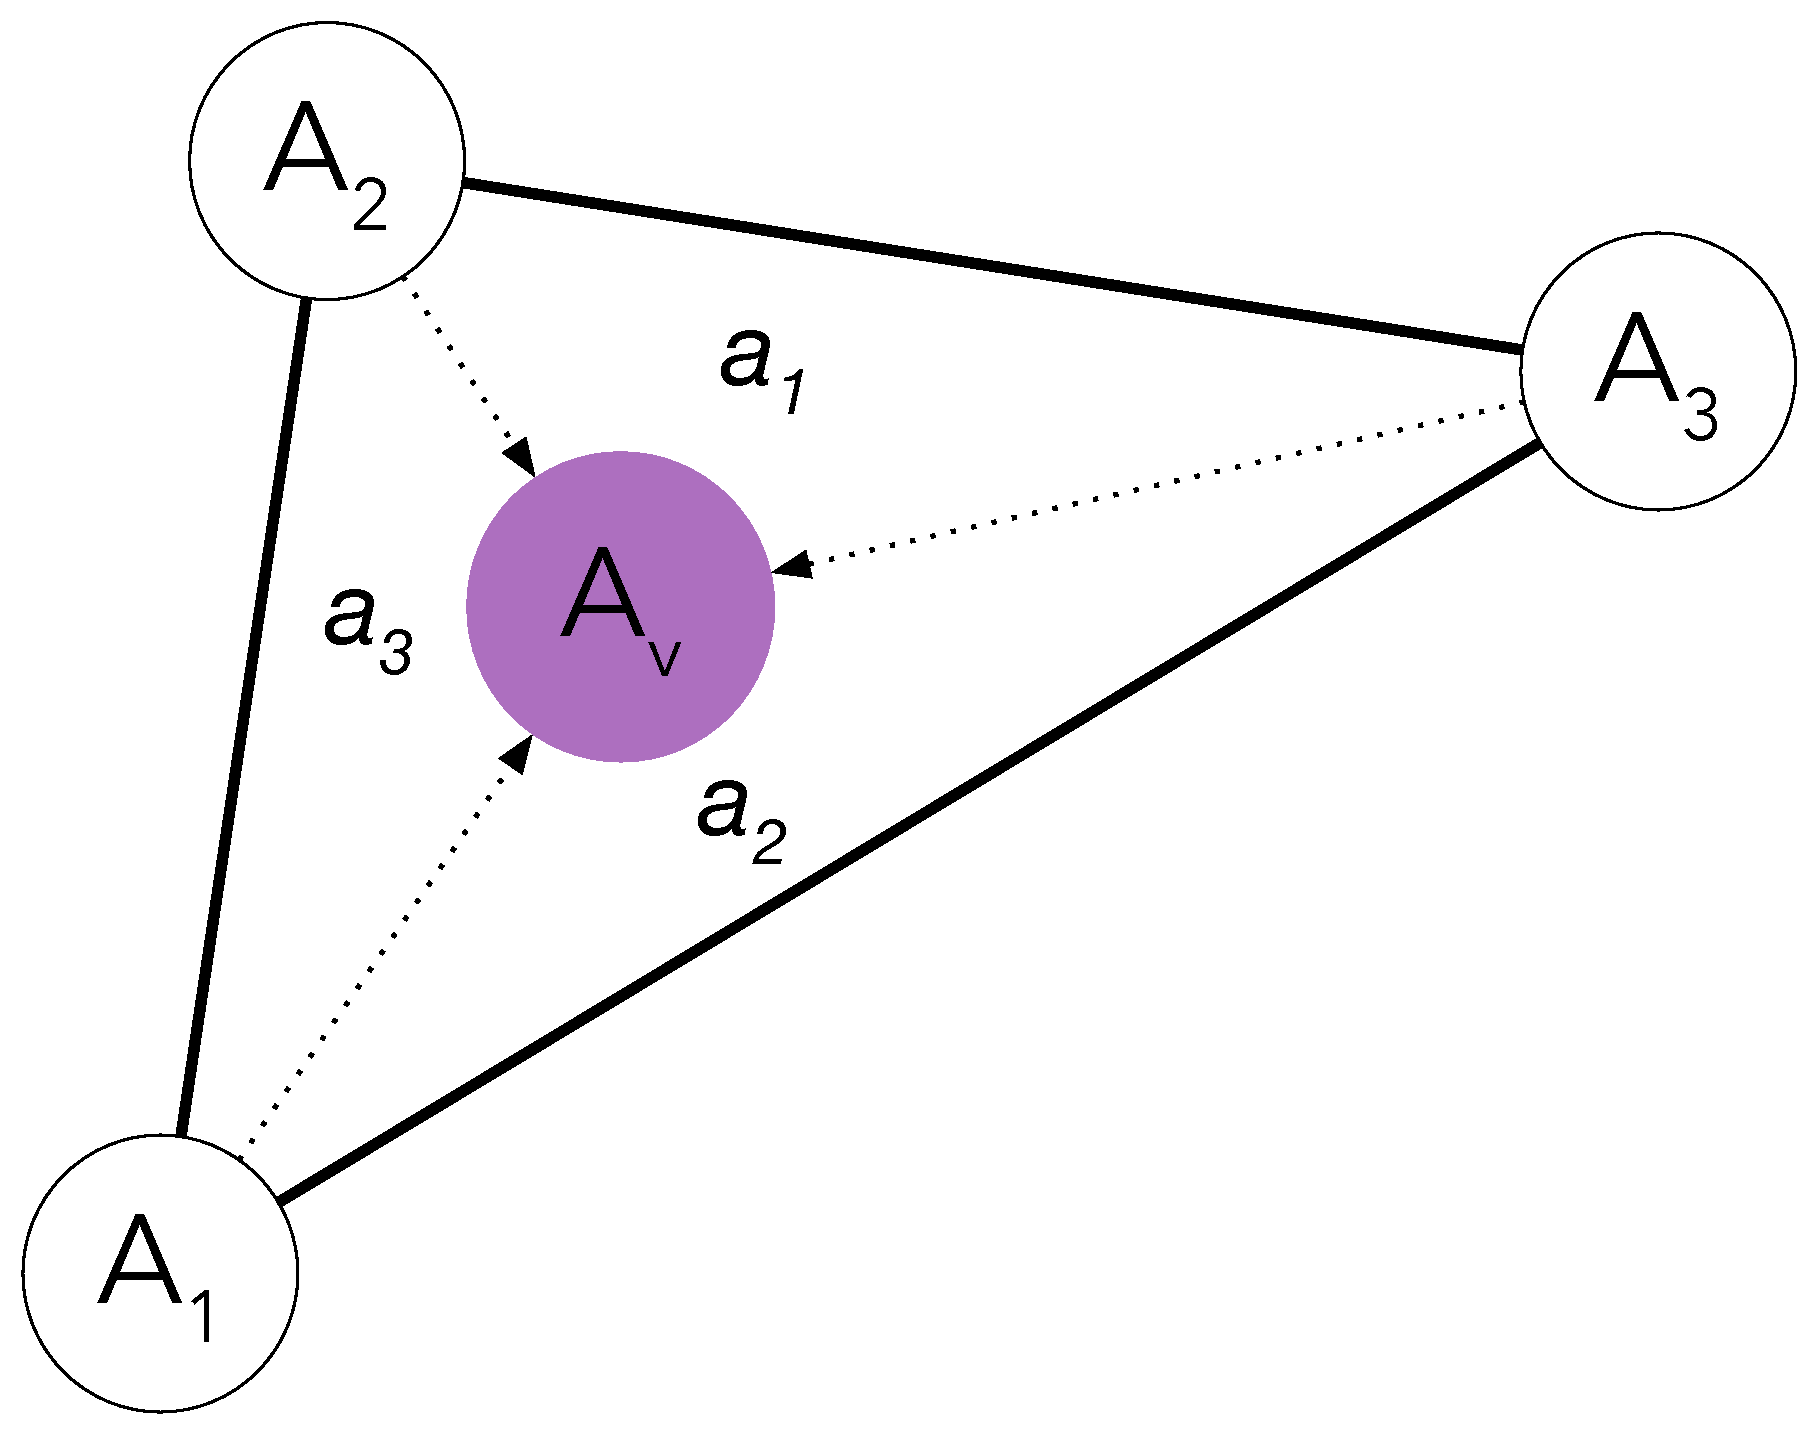
\includegraphics[width=\textwidth]{HA14-RenderingFigure-2015-08-06-1707} 
	   \caption{Barycentric coordinates}
	   \label{fig:rendering:algorithm:barycentric}
    \end{subfigure}
    \qquad
     \begin{subfigure}[b]{0.45\textwidth}
     		\begin{tabular}{l l}
	   	Linear & $A_i = a_i \times A_v$  \\ 
		\\
	   	Log & $A_i = \frac{\log{a_i+1}}{\log{A_{max} +1}}A_v$  \\
		\\
	   	Power & $A_i = \sqrt{a_i} \times A_v$
		\\
		\\
		\end{tabular}
	   \caption{Candidate interpolation methods}
	   \label{fig:rendering:algorithm:interpolation}
    \end{subfigure}
    	   \caption{Interpolation models to determine physical actuator output ($A_{1-3}$) from virtual actuator intensity ($A_v$) and barycentric coordinates ($a_{1-3}$).}
	   \label{fig:rendering:algorithm}
\end{figure}



%%%%%%%%%%
%
%
%
\subsection{Pairwise Comparison Study}

% Our first study is 
%We performed a pairwise comparison between the three candidate interpolation models prototyped for Mango's rendering pipeline.
%Our goal was to determine the user-preferred model for this VT hardware, to be used in Mango's ongoing implementation; and to identify relevant factors (e.g., frequency, amplitude, or individual differences).
To determine the preferred model for this VT hardware in Mango's rendering pipeline, and to identify relevant factors (e.g., frequency, amplitude), %, or individual differences), 
we performed a pairwise comparison of our three candidate interpolation models.

\subsubsection{Participants and Apparatus}
Eighteen volunteers took part (6 female, between age 20-35). % aged 21 to 34) . 
%
The VT hardware consisted of 10 high-quality VT actuators (C2 tactors, Engineering Acoustics, Inc., USA) arranged in a 3-4-3 layout and mounted on the back of a chair in a pad  21 cm high, 29 cm wide, and 2 cm thick;  actuators form equilateral triangles with edges of 6.35 cm  (\autoref{fig:rendering:device}). The rendering engine updates at 100 Hz.
Through piloting, we determined that the device's on-screen visual outline should mirror the sensations rendered on the physical device. That is, if participants see an animation object on the right side of the screen, they prefer to feel it on the right side of the back. 
% (as if they are looking from behind the VT hardware). 
\autoref{fig:rendering:study} shows the experiment interface, in which an arrow represents the sensation direction. 


\begin{figure}[t] %  figure placement: here, top, bottom, or page
   \centering
   \begin{subfigure}[b]{0.37\textwidth}
	   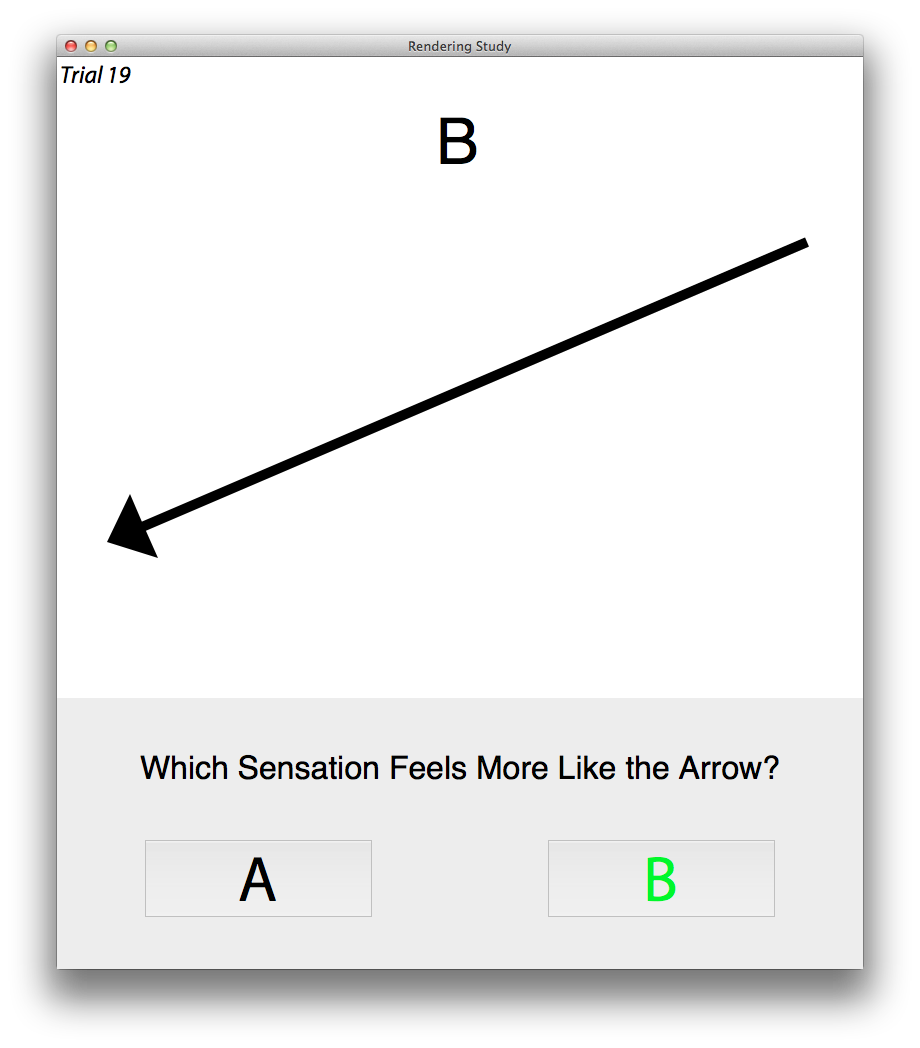
\includegraphics[width=\textwidth]{HA14-RenderingUI-2014-08-19-1417} 
	   \caption{Rendering study interface}
	   \label{fig:rendering:study}
    \end{subfigure}
    \qquad
     \begin{subfigure}[b]{0.55\textwidth}
	   	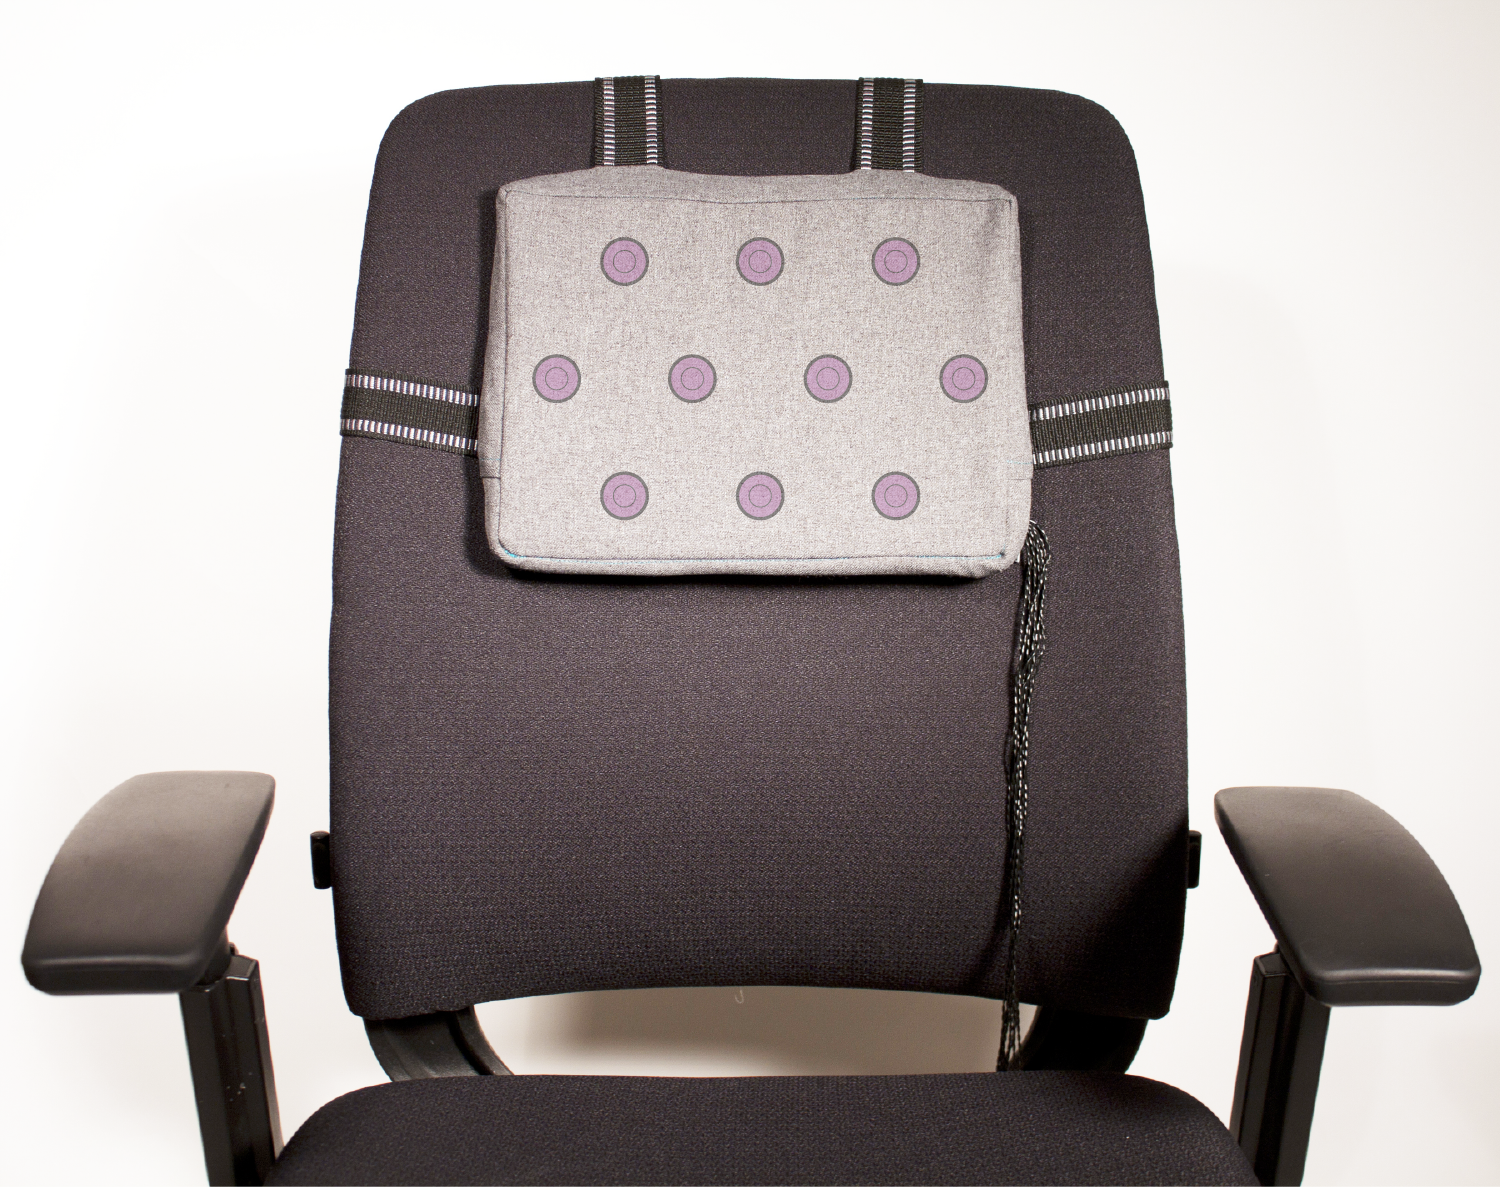
\includegraphics[width=\textwidth]{figure_chairpad} 
	   \caption{Output device with highlighted actuators}
	   \label{fig:rendering:device}
    \end{subfigure}
    	   \caption{Rendering study setup and user interface.}
	   \label{fig:rendering}
\end{figure}

\subsubsection{Methods}
We conducted % a series of 
A/B paired comparison tests (two-alternative, forced-choice) to determine the preferred model out of the three candidates.
%
In each trial, participants were presented with two stimuli at % separated by 
a 400 ms interval.
Each stimulus is
%a rendition of
a ``straight-line" VT stimulation on the back using one model. % of the three interpolation models.
%Stimulus frequency, intensity, direction, and duration were constant across trials. \kmC{slc} % KM 04.12: what is 'across trials'? next para, you refer to these as controlled variables, so I'm a little confused.
Participants were asked to % compare the two stimuli and 
select the stimuli that \emph{best represented straight-line motion} in a variety of directions.

Two durations (500 and 1500 ms), eight cardinal directions, and A/B order were crossed with each model pair, and presented in a random order.
For each trial, frequency was randomly selected from 80, 160, 240, and 300 Hz, and intensity from between 10 and 20 dB above detection threshold.
Each participant performed 96 trials over $\sim$15min (1728 total). 

\subsubsection{Results}
% Analysis was conducted for each pairwise algorithm matchups. % We fit the data
Each algorithm pair's data was fit  to a logistic regression model with participant, frequency, intensity, direction, and duration as factors;  direction was grouped into horizontal, vertical, and diagonal.
We performed stepwise regression (backwards elimination with $\alpha=0.05$ and a $\chi^2$ test for removing each factor) to iteratively eliminate factors that were not statistically significant. % , then analyzed the result.

\emph{Logarithmic vs. Linear.}
% We 
Regression eliminated % 4 factors: 
duration, frequency, intensity, and direction ($p>0.1$).
The resulting model has Nagelkerke $R^2=0.135$.
Using Bonferroni correction for multiple comparisons, 95\% confidence intervals for each participant were computed. 
11 participants were more likely to prefer Log over Linear ($p<0.05$) models; none were likely to prefer the Linear model.

\emph{Logarithmic vs. Pacinian power.}
All 5 factors were eliminated ($p>0.1$).
The overall 95\% confidence interval of participants selecting Log over Power was 37.06\% to 87.40\%, overlapping 50\%.
We therefore detected no significant difference of preference between Log and Power models.

\emph{Pacinian Power vs. Linear.}
We eliminated %3 factors:
intensity, direction and duration ($p>0.1$), with the fitted model's %The fitted model had 
Nagelkerke $R^2=0.0970$.
The confidence interval for each participant-frequency combination, via Bonferroni corrections, yielded 22 / 72 participant-frequency combinations selecting Power model over Linear model more than 50\% of the time.
No one chose the Linear model more than 50\% of the time.

\textbf{Conclusion:}
Logarithmic interpolation outperformed linear and was % found 
equivalent to Pacinian power model. We proceeded with the logarithmic model for Mango's implementation, as the power model did not outperform either of the others. % the linear model.
%\kmC{ based on its greater simplicity of implementation. ???}
% Of the three candidate algorithms, we chose the Logarithmic interpolation method for the rendering algorithm of the Mango animation tool. 

%%%%%%%%%%
%
% Animation Tool Evaluation
%
\section{Design Evaluation}
% We implemented the critical functional features of Mango as described in the above sections.
To evaluate Mango's % the 
animation metaphor and expressive capability,
%with critical functional features implemented,
we asked media professionals to
% we had media professionals 
create a variety of designs.
Qualitative evaluation was chosen for rich, focused, early feedback of the animation metaphor and lessons for iteration.
A quantitative comparison between tool perspectives is left until more refined tools are developed.
We wanted to establish whether this is an effective approach before studying the most effective approach.


Six participants (P1-6, 3 females) were introduced to Mango driving % linked to 
the  VT hardware described previously. % for the pairwise comparisons. 
%First, each participant was interviewed about their background.
P1 had experience with haptics but not animation beyond video editing;
P2-5 had animation experience but little or no experience with haptics;
P6 had no experience with haptics or animation, but was familiar with media tools like Adobe Photoshop.
P5 was also involved with the requirement gathering interviews presented earlier.
Each entire session took 40 to 60 minutes.


Each participant was introduced to Mango with a training task: % and the use of tactile animation objects and vector sensations.
designing an alerting sensation using %  ``alert" sensation with 
either animation objects or vector sensations (order counterbalanced).
%half of them used the animation objects first and the other half used vector sensations first.
Then, each participant was given three design tasks.
1) Primarily \emph{temporal}: create a heartbeat sensation.
2) Primarily \emph{spatial}: tell a driver to turn left.
3) \emph{Context-based}: create a tactile animation to match a sound file.
A 3-second sound effect of a bomb falling (with a whistle descending in pitch) then exploding with a boom was chosen, i.e., complex with two semantic components.
The wide array of resulting designs can be found in the accompanying video.
Mean non-training task time was 5:59 (med 5:38, sd 2:46, range 1:41-13:48).

After each task, participants rated confidence in their design from 1 (Not confident) to 5 (Very confident), primarily to stimulate discussion.
All designs were rated 3 or higher; P6 wrote ``6" for his sound-based design.
The animation object training task was always rated the same or higher than the corresponding vector training task.
While suggestive, these ratings were self-reported and from a small sample.
We thus did not conduct statistical analysis.
%, due to small sample size.

%
% Show one animation
%
\begin{figure}[htb] %  figure placement: here, top, bottom, or page
   \centering
%   	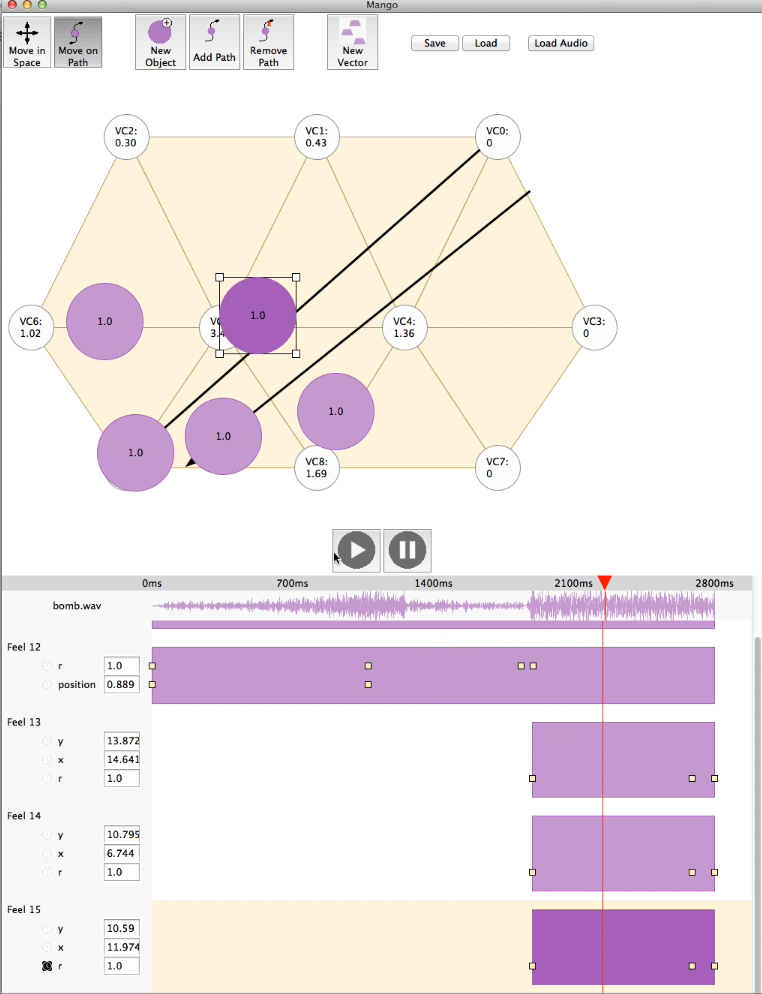
\includegraphics[clip=true, trim= 1 150 0 7, width=0.4\textwidth]{P2_sound_example-2014-09-22-1630} 
	   	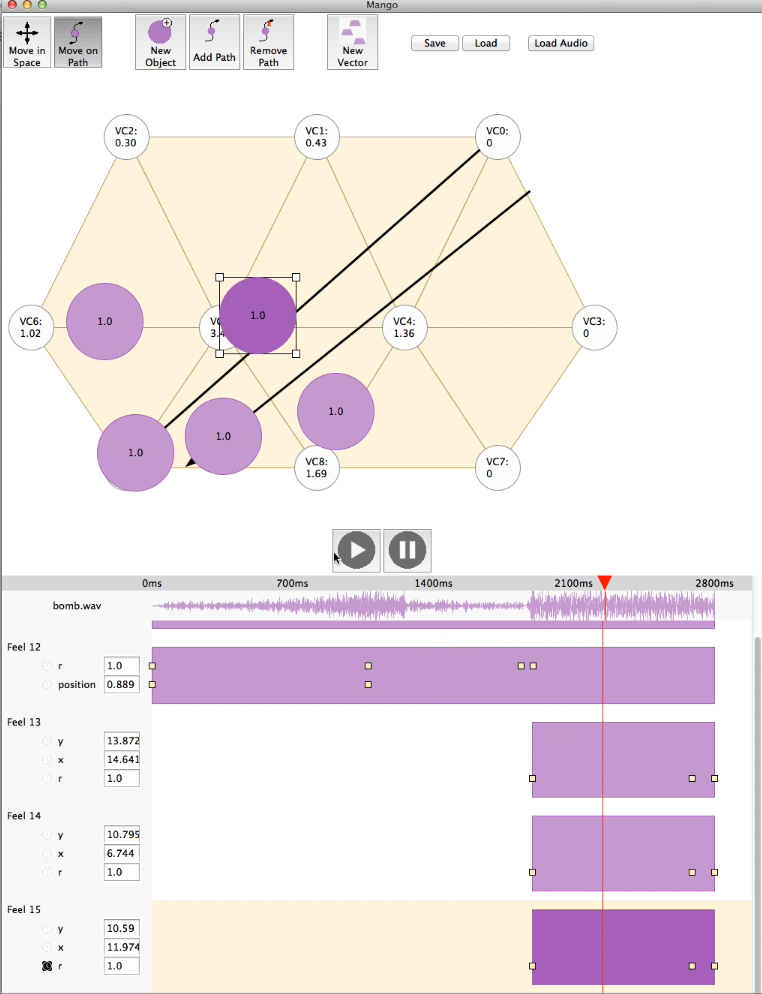
\includegraphics[clip=true, trim= 4 155 0 85, width=0.8\textwidth]{P2_sound_example-2014-09-22-1630} 

	\caption{Example of P2's animation for matching a sound. See the accompanying video for all participant animations.}
	\label{fig:animation:example:p2}
\end{figure}




A semi-structured interview followed the design tasks.
%The interviewer then followed up on interesting statements and/or concerns.
Participants were asked to compare animation objects with vector sensations, and to walk through the interface to elicit feedback.
%
% Study 2 results
%
%\subsection{Results}
Interviews were conducted and analyzed by a researcher with training and experience in qualitative research, and followed established methodologies:
% by considering each statement, memoing, coding, and relating codes
%according to % Corbin and Strauss's 
methods of grounded theory  \cite{Corbin2008} informed by phenomenological protocols \cite{Moustakas1994}.
Analysis resulted in four themes.

\subsubsection{Theme 1: Animation Metaphor}
Participants found the tool easy to use.
All six participants were able to accomplish all five tasks (object alert, vector alert, heartbeat, turn left, sound).
Participants described the interface as intuitive (P1-5), agreeing that it was an animation tool: \qq{It's up to the standards of other animation tools}{P1}, \qq{This is totally animation}{P2}, \qq{It felt very much like an animation tool}{P4}, \qq{I'm not an expert when it comes to haptics, but this software seems almost as if it can change the game of designing haptic vibrations}{P5}.
Negative feedback focused on polish and feature completeness:
% not implementing enough features of their preferred tools and general feedback on polish and streamlining of the interface:
\qq{gotta spline [the keyframe interpolation]}{P2}, \qq{a couple quirks but there was nothing difficult to overcome}{P4}, \qq{being able to design your own curve [path] would be really nice}{P5}.
%, \qq{move in space and move on path can be one thing}{P6}.


\subsubsection{Theme 2: Tactile Animation Object vs. Vector Sensations}
Participants relied more on animation objects %  used animation objects more frequently
than vector sensations, which
%Vector sensations 
were only used twice: P4's heartbeat task and P5's sound task (combined with an animation object).
P1 switched from vectors to animation objects early in her heartbeat task;
%for her remaining tasks
no other participants used vector sensations.


Animation objects were described as easier to use and more intuitive, especially to represent location or for non-animators. \qq{After using the new object I'd probably never use new vector again}{P2}, 
%especially to describe motion or position:
\qq{easier to find the location of the heart}{P1}, 
%They were also described as more appropriate for people without animation experience:
\qq{if I weren't an animator I think I would only use [animation objects]}{P4}.
%, \qq{You have to be a little more careful when animating [vector sensations]}{P5}.
%
%Animation objects and vector sensations supported different workflows. Animation objects tended to be described as better for position, movement, and for % if you wanted to have 
%multiple objects, while 
Vectors were preferred for more fine-tuned control when motion didn't matter as much, often using many keyframes.
\qq{You can control multiple [actuators] at the same time, so you don't have to create new objects and then put them everywhere on the screen}{P1},
\qq{[Animation objects] can be more comfortable to use when one doesn't work with keyframes}{P3}, 
\qq{If you want precise control over [actuators], then vector is the way to go}{P4}.
%Participants rarely combined the two:
%\qq{I'm already into the object mode, I forget about the vector}{P6}.

%
% Shows three animations
%
%\begin{figure*}[htbp] %  figure placement: here, top, bottom, or page
%   \centering
%      	\begin{subfigure}[b]{0.30\textwidth}
%		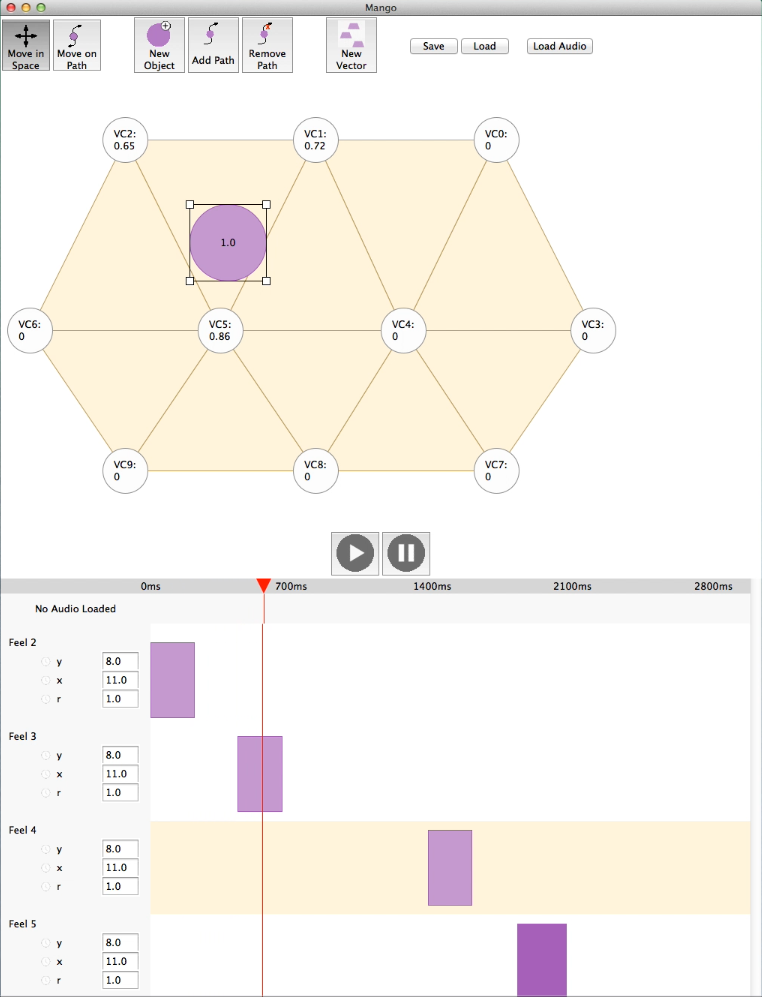
\includegraphics[width=\textwidth]{p1-heartbeat-example} 
%		\caption{Heartbeat task by P1}
%		\label{fig:animation:example:p1}
%	\end{subfigure}
%	\quad
%	\begin{subfigure}[b]{0.30\textwidth}
%		   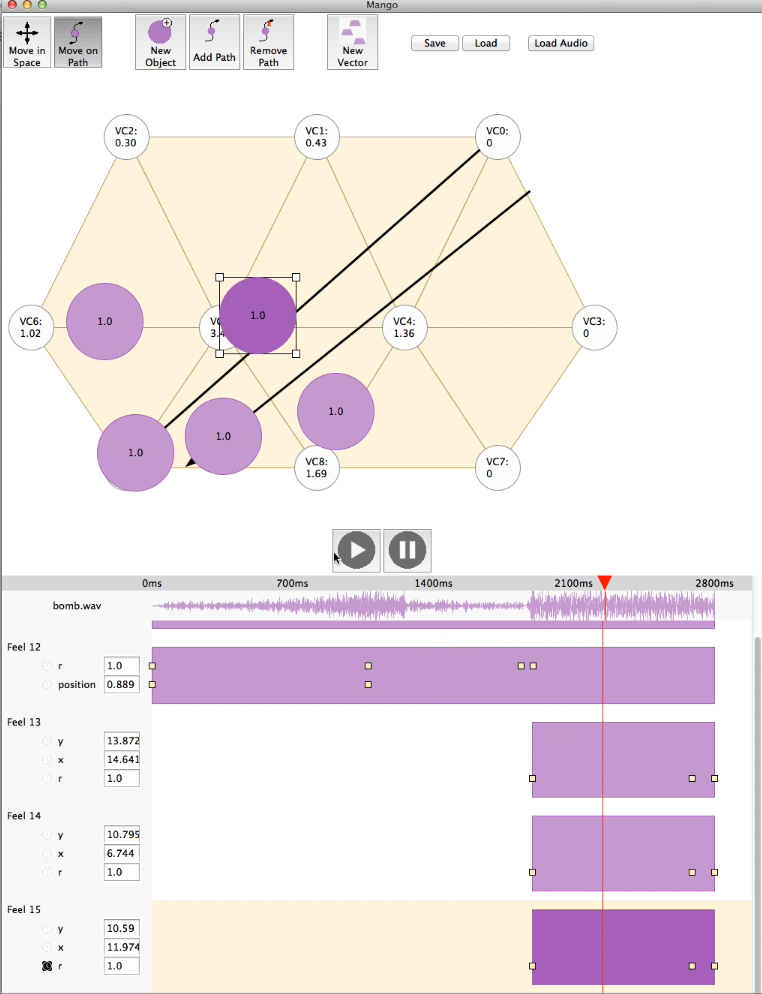
\includegraphics[width=\textwidth]{P2_sound_example-2014-09-22-1630} 
%		   \caption{Sound task by P2}
%		   \label{fig:animation:example:p2}
%	\end{subfigure}
%	\quad
%	\begin{subfigure}[b]{0.30\textwidth}
%		   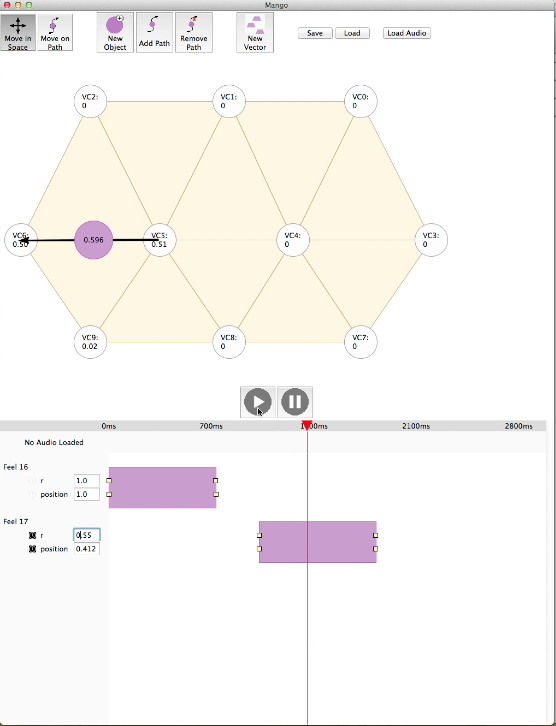
\includegraphics[width=\textwidth]{p4-turnleft-example-2015-01-19-1024} 
%		   \caption{Turn left task by P4}
%		   \label{fig:animation:example:p4}
%	\end{subfigure}
%
%
%
%
%      	\caption{Examples of Animations}
%	\label{fig:animation:example}
%\end{figure*}


%\theme{4}{Feedback, Context and Imitation}
\subsubsection{Theme 3: Designing-in-action with direct manipulation}
Participants used direct manipulation to feel their designs in real time, %  was valuable to participants.
dragging animation objects %in the animation window
and scrubbing through
%at various speeds in
the timeline: \qq{I would make the [animation] object and just play around with it before creating the animation, as a way to pre-visualize what I was going to do}{P5},
\qq{I kind of play around with it, and randomly come up with the ideas}{P6}.
P2 even noted that YouTube did not have
 real-time video scrubbing feedback like Mango's:
 %support for haptic and audio feedback:
 \qq{I wish I could scrub back and forth [with YouTube]}{P2}.
However, continual % constant 
vibrations were annoying, and participants requested a ``mute" feature:
%A VT feedback ``mute'' would be welcomed.
%P4 and P5 moved the timeline so that no output would play during design phase. 
% was playing while they were in design phase.
%\qq{It would be nice if when I [enter values into text fields] it doesn't go off constantly, it's getting annoying}{P3}.
\qq{It would be nice if...it doesn't go off constantly.}{P3}.
%It was further suggested that each object should be independently mutable (as in hiding Photoshop layers), and VT output should be mutable entirely. 

More generally, participants used feedback from their experience or external examples.
P1 stopped to think about her own heartbeat,  P2 used a YouTube video of a heartbeat as a reference, and P3 based her alert on her phone: %directly stated that she
%used imitation for the non-sound tasks
%;  her alert consisted of two vibrations similar to her phone: 
\qq{It's typical to have two beeps for mobile phones}{P3}.
Correspondingly, participants were excited when prompted by an audio sensation: \qq{I was really happy with the bomb one, because I could really hear it and imagine me watching a TV and then feel it at the same time}{P1},
\qq{The sound part was good, that would be a fun thing to design for}{P4}.



\subsubsection{Theme 4: Replication through Copy and Paste}
Replication in both space and time was common while using Mango.
Many designs had symmetrical paths to reinforce sensations (\autoref{fig:animation:example:p2}).
All but P4 requested copy / paste as a feature.
%, suggesting it would be useful (P2, P3), faster (P1, P2) and easier (P5).
%P1, P2, and P5 wanted to duplicate their heartbeat sensation to be multiple beats, but did not do so without copy and paste.
%, instead saying they would repeat or loop it. [??????]
\qq{I could just copy/paste the exact same thing on the left side and then move it to the right side}{P1}, \qq{I have the timing the way I like it, ideally it'd be cool if I was able to copy and paste these, so it would be able to repeat}{P5}.
%\qq{Is there any way to copy and paste keyframes?}{P2}.

\section{Discussion}
Here we interpret our design evaluation, explore animation with other devices, and describe applications and limitations.

\subsection{Design Evaluation Summary}
From our design evaluation, we conclude that tactile animation is a promising approach for controlling tactile grids.
Direct, continuous manipulation of tactile animation objects supported embodied design and exploration by animators, who rapidly iterated on designs to try new ideas.
Mango facilitated the design of a wide variety of animations (see accompanying video) and received positive responses.
We also found recommendations for our next iteration: more animation features, video as well as audio context, and muting.% (similar to hiding layers in Photoshop).%'s ``hide layer'' functionality).

\begin{figure}[htb] %  figure placement: here, top, bottom, or page
   \centering
   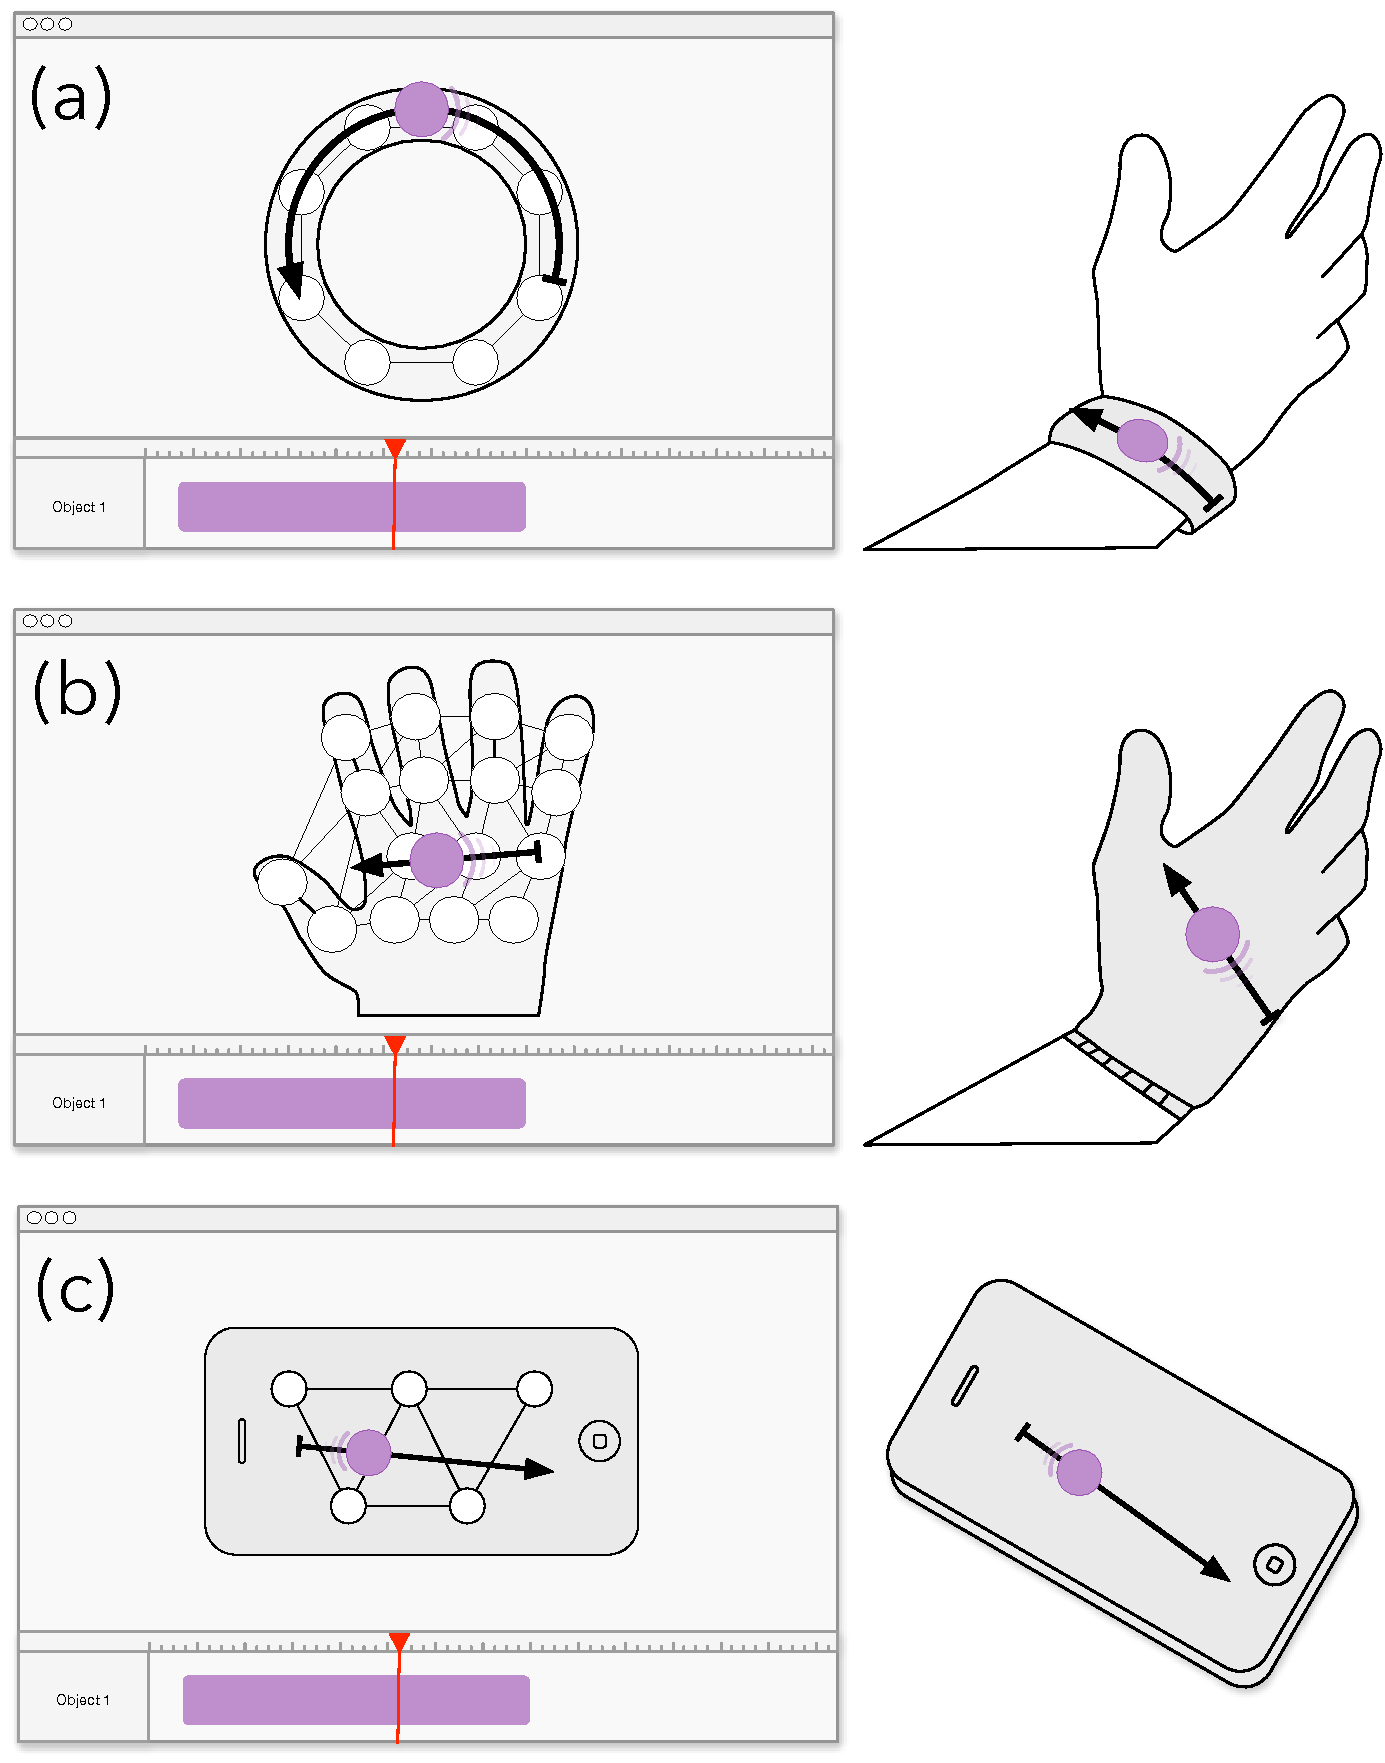
\includegraphics[height=2.75in]{HA14-Applications-Split1-2015-04-14-1025} 
%   \caption{Tactile animation could define motion with (a) 1D actuator arrays, (b) dense and sparse VT grids, (c) handhelds.}
%   \label{fig:application:space}
%\end{figure}
%\begin{figure}[htb] %  figure placement: here, top, bottom, or page
%   \centering
\qquad
   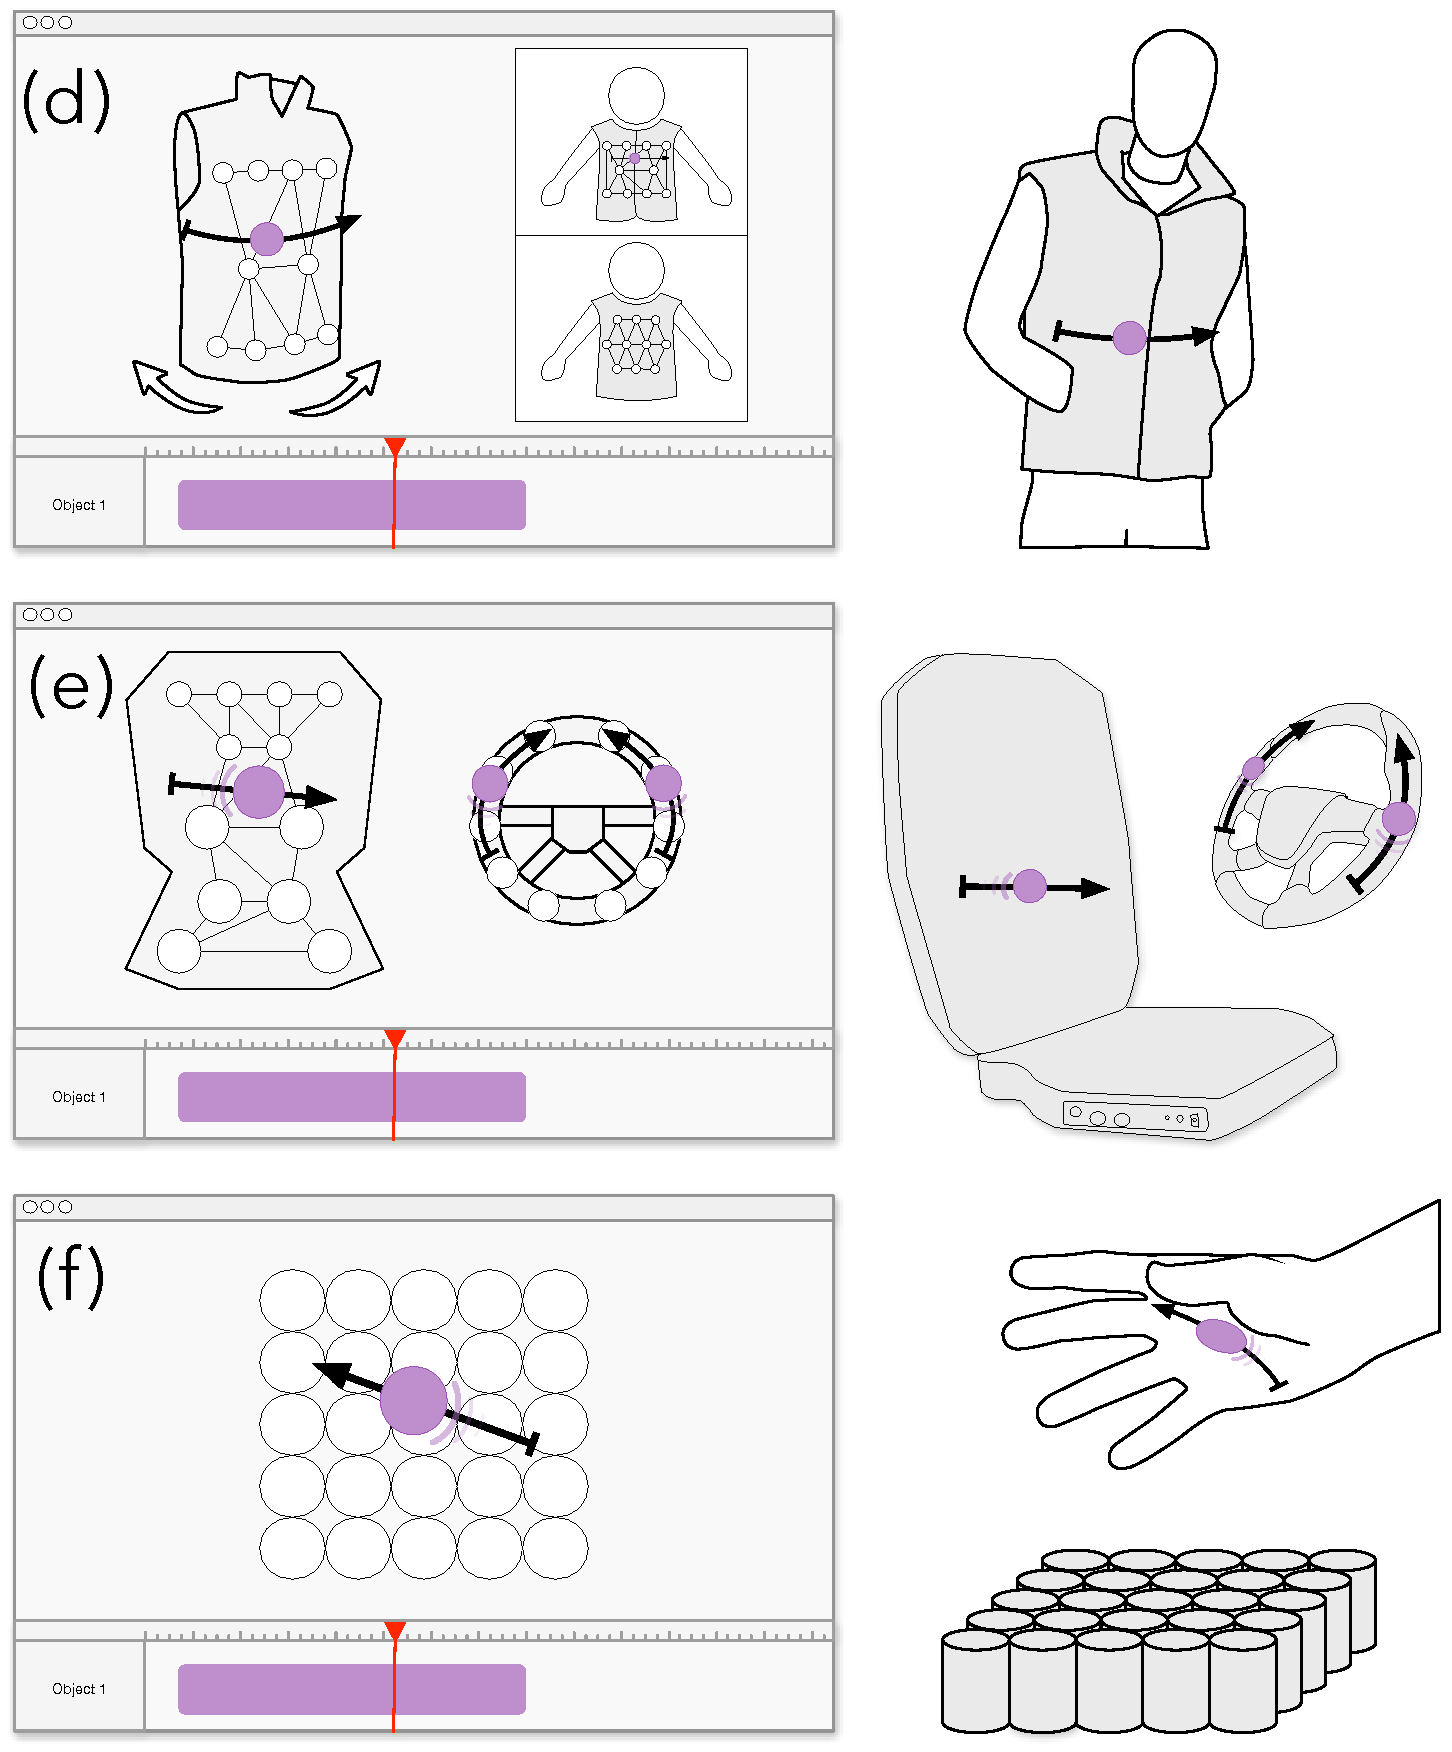
\includegraphics[height=2.75in]{HA14-Applications-Split2-2015-04-14-1025} 
%   \caption{Tactile animation could also define motion  with (d)  3D surfaces, (e) multi-device contexts, and  (f) non-VT devices like mid-air ultrasound.}
%   \label{fig:application:space}
      \caption{Tactile animation could define motion with (a) 1D actuator arrays, (b) dense and sparse VT grids, (c) handhelds, (d)  3D surfaces, (e) multi-device contexts, and  (f) non-VT devices like mid-air ultrasound.}
   \label{fig:application:space}
\end{figure}

%\vspace{20pt}
\subsection{Possible Extension to Other Device Classes}
%\emph{Future Work: Applications and Extensions}\\ % Application space }\\
%We look forward to extending Mango to other devices.
% Mango is not limited to
The animation metaphor is not limited to a back-based pads.
Part of the advantage of an abstracted animation object is that, 
as long as a suitable rendering algorithm can be developed, the metaphor can apply to other devices.
In this section, we illustrate possibilities that we plan to explore in future work.


\emph{1D VT Arrays (\autoref{fig:application:space}a)}:
1D VT arrays are common in arm sleeves, wrist bands, belts, and similar wearables.
These devices provide sensations along the path of the array.
By constraining objects to a linear or circular path, barycentric coordinates collapse into 1D interpolation.

\emph{Dense and Sparse VT Grids  (\autoref{fig:application:space}b)}:
2D VT grids are also common, used in chairs, gloves, and the backs of vests.
%Dense arrays previously had their own actuator-based authoring tools \cite{Kim2009}.
While we evaluated Mango with a sparse back-mounted array, tactile animation naturally supports denser arrays, either with our rendering algorithm or by using a nearest-neighbour technique to activate a single actuator.
%; in both cases, animation objects can be directly manipulated.
%In the present work, we evaluated the usability of Mango to author variety of VT sensations on sparse arrays.
%The actuator layout in both these devices are dif- ferent, and we accomodated them by selecting an appropriate
%algorithm and layout to render high definition haptic feedback.


\emph{Handhelds (\autoref{fig:application:space}c)}:
Actuators embedded in handheld objects, such as mobile devices, game controllers, or steering wheels, shake objects instead of directly stimulating the skin.
Animators might be able to define source locations for vibrations using handheld-based rendering algorithms (e.g., \cite{Seo2013}).
%Similarly, a single embedded vibrator in handheld devices can be supported by constraining the tactile object to a single point.


\emph{3D Surfaces  (\autoref{fig:application:space}d)}:
Mango currently only supports a 2D location for its animation objects.
However, tactile animation can be extended to support surfaces of 3D surfaces, such as vests or jackets that wrap around the user's body. 
More work will need to be done to perfect this interaction style, possibly using multiple views or a rotatable 3D model with animation objects constrained to the surface.
%, drawing more from 3D animation tools like Maya.

\emph{Multi-device contexts  (\autoref{fig:application:space}e)}:
Mango's rendering algorithm already supports connections to multiple devices simultaneously.
The editing interface could combine layouts for different devices, enabling animators to animate the entire user experience (such as a car's seat and steering wheel).

\emph{Non-vibrotactile devices (\autoref{fig:application:space}f)}:
While our rendering algorithm is particular to VT arrays, a tactile animation object can represent manipulable percepts with other actuation technologies.
%Mango is not limited to only VT devices, similar to the one used in the present evaluations.
Ultrasound-based mid-air displays generate a sensation as a focal point with a position and size \cite{Wilson2014}; this sensation could be manipulated through a tool like Mango.
% produce a percept of object in mid-air and can be manipu- lated by changing the focal point as a animated object on the Mango interface. Algorithm to generate localize percept can be loaded along with the specifications written in the config- uration file.
Similarly, passive force-feedback sensations (e.g., Hapseat \cite{Danieau2012a}) or height displays (a grid of pins) could be supported.


%Beyond the VT pad used in our evaluations,
%the animation metaphor naturally supports other devices, some of which have been controlled by other authoring tools (\autoref{fig:application:space}).
%By constraining animation objects to a circular path, wristbands and belts can be supported (\autoref{fig:application:space}a).
%Dense, regular displays, such as glove-based grids \cite{Kim2009}, could also be controlled with direct manipulation (\autoref{fig:application:space}b).
%An extension to vests and other cylindrical or spherical displays might use multiple views to facilitate design (\autoref{fig:application:space}c).
%Finally, complex multi-device scenarios can be coordinated in a single interface (\autoref{fig:application:space}d).
%We have already extended Mango to support a chair-based display (similar to \cite{Israr2011a}), with planned extensions for vests and gloves (\autoref{fig:devices}).

\subsection{Interactive Applications}
While our goal was to enable animators to create rich content, the tactile animation object can be linked to alternative input sources for other interactive experiences.

\emph{User gestures.}
User gestures and motion can be tracked and mapped to animation objects directly rendered on the haptic hardware.
For example, a user creates patterns on a touch sensitive tablet that maps touch locations to a grid.
Users could play games or create personalized haptic messages on the back of a vest.
Similarly, a dancer's movements could be tracked through accelerometers, drawing animated haptic content on the body of her audience through actuated theater seats during a live performance.
%Object location and parameters could be linked to a mobile or gestural input method; we have implemented tactile animation objects on a tablet interface (\autoref{fig:tabletinput}).
%Other media like a video or audio streams could be linked to objects to automate the process; computer vision techniques

\emph{Camera feed extraction.}
%Objects from Camera Feed
Motion from video feeds can be automatically extracted with computer vision and rendered on grid displays \cite{Kim2014}, providing dynamic patterns associated with actions during sports, movies, and games.
Similarly, animation parameters could be extracted and mapped to positions on a VT grid, creating haptic feedback for non-haptic media.
%Animation Model
%Animators can create animated models on their preferred tools and export them in a standard file format. The file is opened by a playback tool and renders dynamic haptic pat- terns on grid displays. For example, an animated sequence is directly translated to moving tactile patterns during mid-air user interactions, as shown in FIG??.

\emph{Data streams.}
One main application of haptic grid displays is to provide users directional, assistive, and navigational cues during driving cars, walking down the street, or with over-
saturated sensory tasks.
%Our rendering pipeline and its psy- chophysical assessment illustrates a technique to 
Users could associate digital data streams, such as GPS input, to predefined set of directional patterns on the back or palm of the hand.
%Designers, engineers, scientists and students can utilize our techniques to integarte animated haptic content in their projects; such as stock market feeds (anonymous). Such data feeds could be used in vest and jackets to assist blind indi- vidual during navigation, and over-stimulated indivual during task completion.



%
%\begin{figure}[htb] %  figure placement: here, top, bottom, or page
%   \centering
%   \begin{subfigure}[b]{0.235\textwidth}
%	   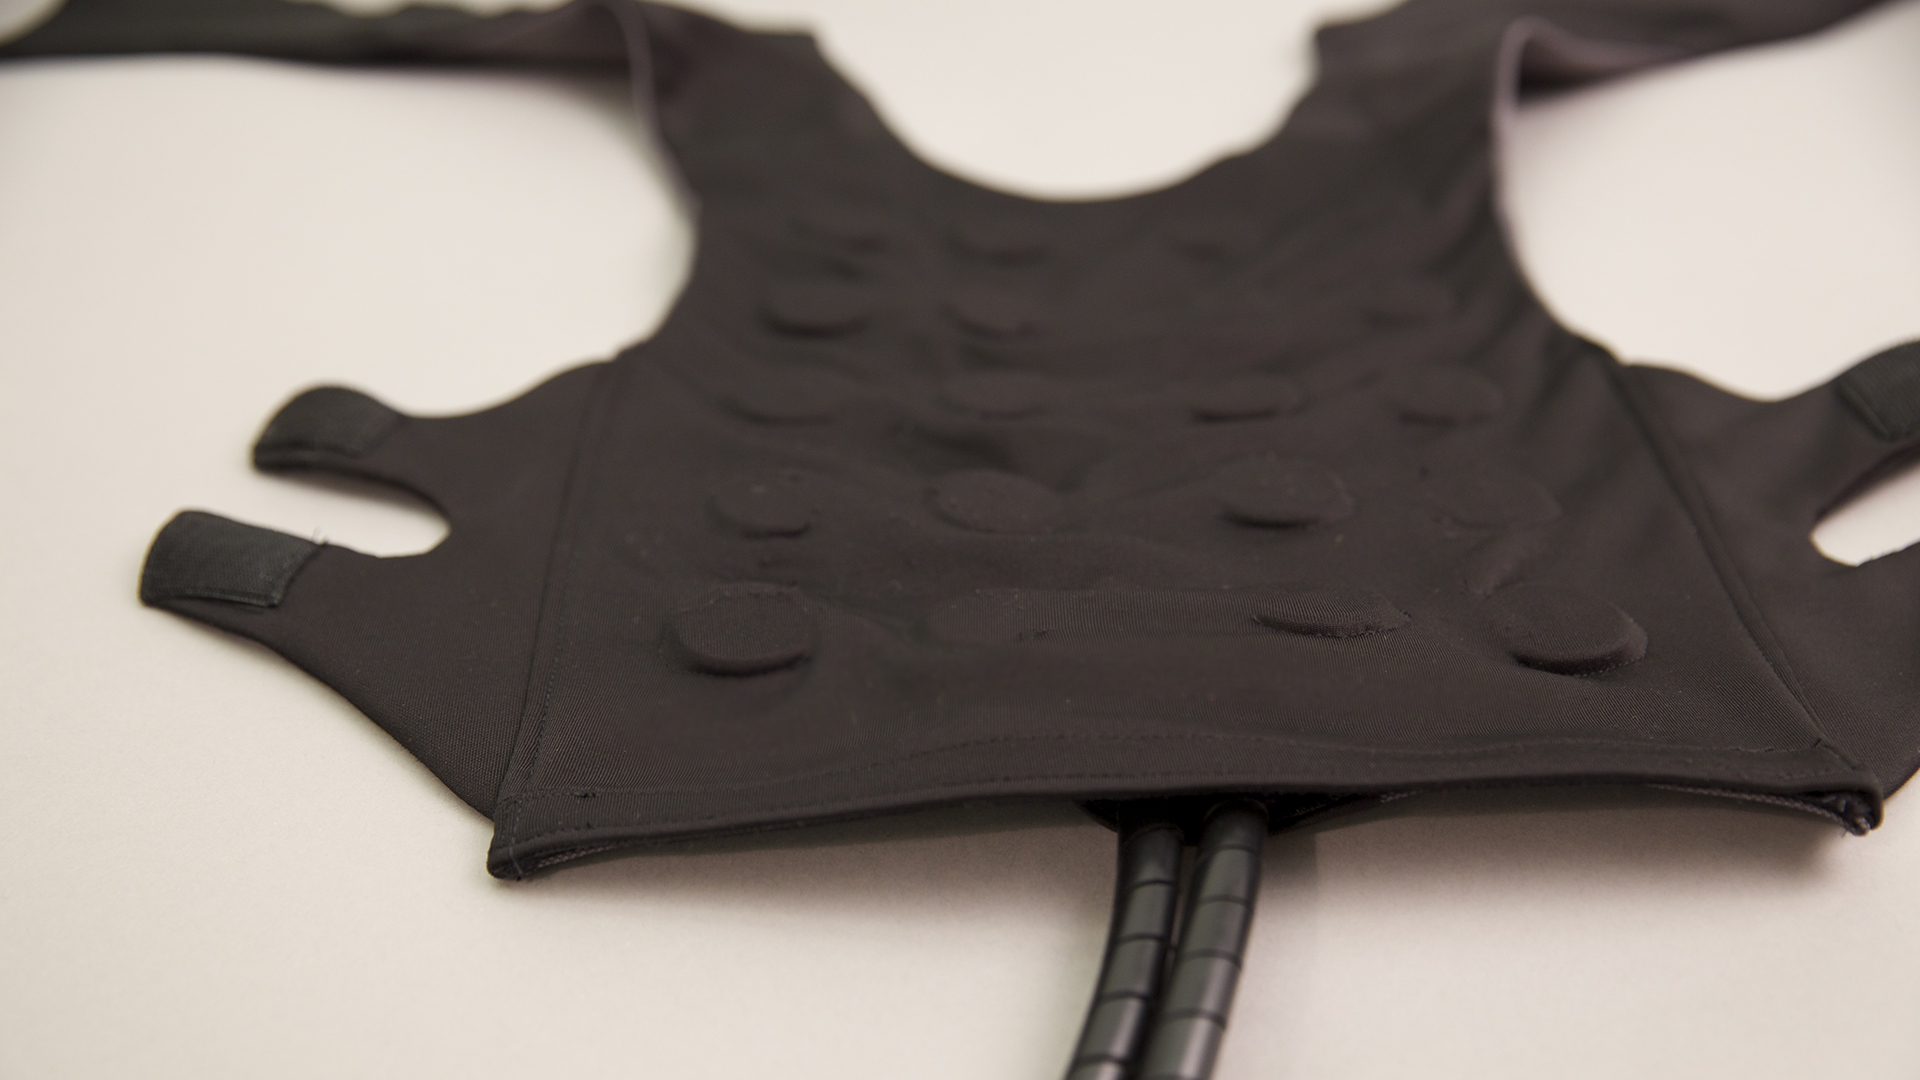
\includegraphics[width=\textwidth]{vest4} 
%	   \caption{Vest}
%	   \label{fig:devices:vest}
%    \end{subfigure}
%     \begin{subfigure}[b]{0.235\textwidth}
%	   	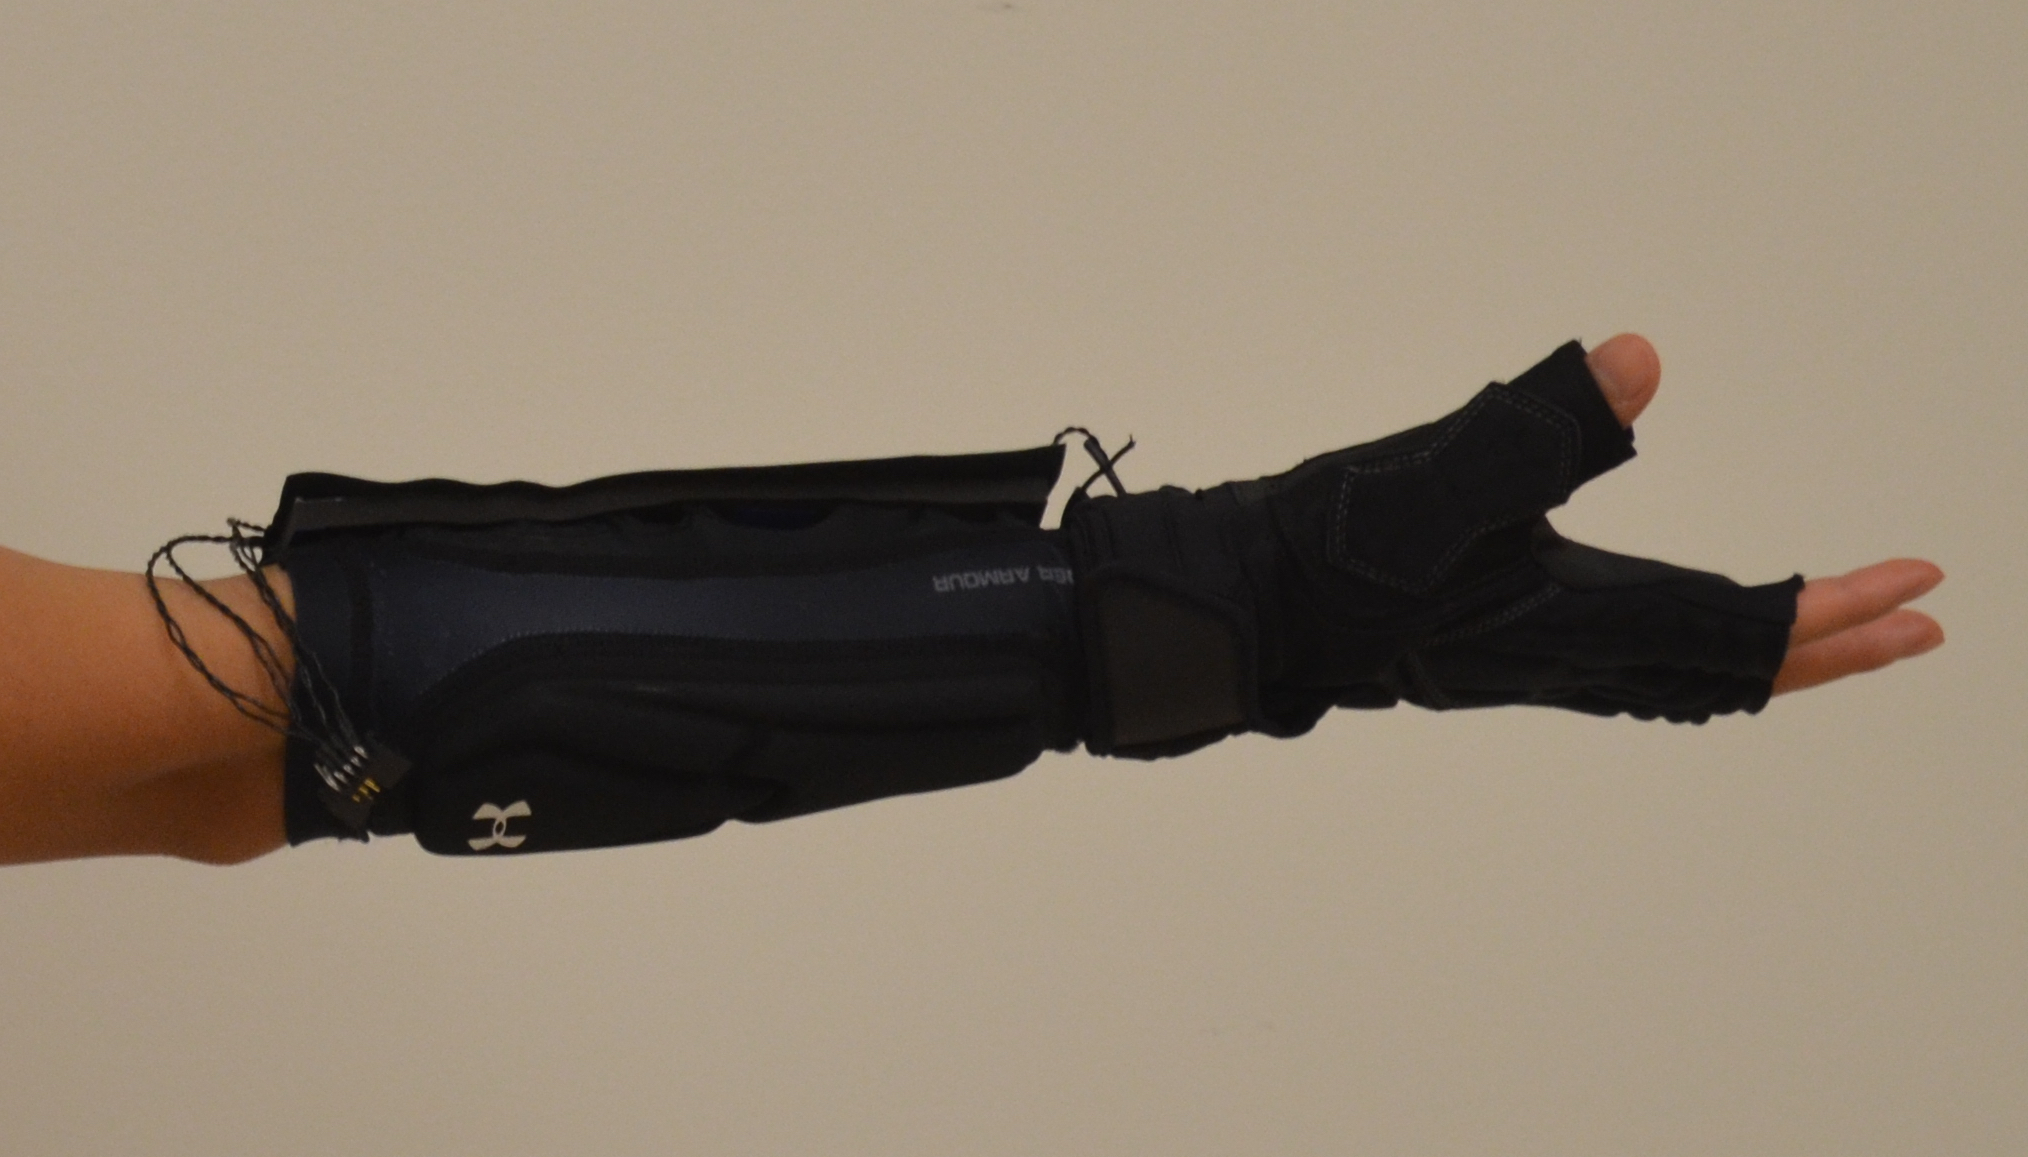
\includegraphics[width=\textwidth]{glove} 
%	   \caption{Glove}
%	   \label{fig:devices:glove}
%    \end{subfigure}
%    	   \caption{Other supported devices.}
%	   \label{fig:devices}
%\end{figure}


%\begin{figure}[htb] %  figure placement: here, top, bottom, or page
%   \centering
%	   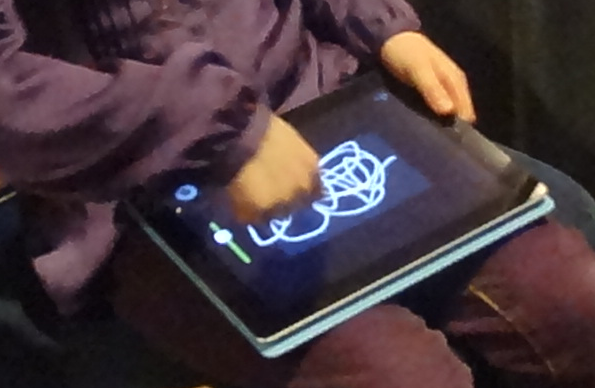
\includegraphics[width=0.47\textwidth]{tablet-input} 
%        	   \caption{Tactile animation objects implemented on a tablet.}
%	   \label{fig:tabletinput}
%\end{figure}



\subsection{Limitations}
While the tactile animation metaphor seems promising and may apply to many contexts, it is limited by the requirement of a suitable rendering algorithm for target hardware.
We have not yet explored other form factors, such as handhelds, multi-device scenarios, or non-vibrotactile sensations.
Although we perceptually optimized our algorithm, we did not conduct a full psychophysical investigation.
Further work needs to be done to identify the limits, thresholds, and peculiarities of this rendering technique.
Examples include:
curved trajectories of animation objects (although participants' use of curved motion was encouraging, e.g., P5's turn left sensation),
spatial frequency control (how to superpose animation objects of differing frequencies),
non-triangular meshes (e.g., quadrilateral interpolation or kernel methods),
and mixed actuator types (such as a chair with both voice coil and rumble motors, \autoref{fig:application:space}e).

%%%%%%%%%%
%
%Implications for Design
%
%%%%%%%%%%
\section{Conclusion}

%This paper presents Mango, a new tactile animation tool to create rich, dynamic and expressive haptic experiences. 
%The tool utilizes animation metaphor in the design process and renders animated VT patterns on a variety of spatial VT displays.
%Design requirements gathered in interviews and literature review are implemented on a prototype software that was evaluated with artists and a normal everyday computer user.
%The post evaluation interviews and feedback suggested that the tool was useful and easily adaptable; and participants highly preferred animation metaphor to design haptic patterns.
%Overall, tactile animation represents a promising new direction to support haptic media design.

%A key feature of Mango is that it can be used with a wide range of haptic feedback hardware. The hardware specific definitions are provided in the configuration file which facilitates authoring of animations and its rendering on the hardware. Configuration files for new hardware can be constructed and loaded in Mango, to use its authoring capabilities with new hardware.  

%\kmC{Adjust weight: tactile animation then Mango} % Km: up to here, I think it's consistent now. I ran out of steam.
This paper introduces the \emph{tactile animation object}, a new abstraction for creating rich and expressive haptic media on grid displays.
% The design of Mango is derived from an
This animation metaphor allows designers and media artists to directly manipulate phantom vibrotactile sensations continuously in both space and time.
Our rendering pipeline, which uses a perceptually-guided phantom sensation algorithm, enables critical real-time feedback for designing.
%an approach that is more direct and potentially creative than coordinating individual actuators, and which scales better to large actuator maps, where perceived motion is nearly intractable using track-based approaches.
%Unlike previous tools that either required rigorous programming background or was applicable to a specific hardware configuration, an animation approach also % our tool
%provides a familiar interface to a large animation workforce, therefore eliminating training time and cost necessary for haptic content production in the mainstream media.  
We incorporated these ideas into a prototype, Mango, with a design grounded in animator requirements and haptic design guidelines.
Professional animators used our tool to create a variety of designs, giving positive feedback and excitement for future versions.
This approach has the potential to % KM: concerned that this functionality can be added to any tool with properly designed configuration files, and isn't tied particularly to the other innovations reported here. If so, need to be much more careful about how it's phrased since this capability isn't even really demonstrated here - you only use one display apparatus.
% Moreover, Mango 
accommodate a large variety of haptic hardware, ranging from a single shaking element mounted on the seat to an array of actuators stimulating multiple points on the skin, and can export content into formats applicable in the production pipeline.
Tactile animation empowers animators with a new set of artistic tools for rich, multimodal feedback. 

\section{Acknowledgments}
We thank our reviewers and participants for their valuable feedback.
This work was supported by Disney Research, with
additional support provided by NSERC.
%Oliver holds an NSERC CGS D scholarship.


%
%
%\subsection{Demo}
%\osC{Add image, description, takeaway from demo}
%
%\section{Discussion}
%The Tactile Animation project expanded our understanding from the Haptic Instrument study in \autoref{ch:hapticinstrument}.
%Specifically, it reaffirmed the value of real-time feedback and the need for examples, and showed that a persistent object model reduces cognitive load.
%It also suggests again that examples and user experiences are extremely valuable to the design process, providing motivation for example-based haptic design discussed next in \autoref{ch:hapticexamples}.
%
%
%
\endinput





\chapter{Combine: Macaron}
\label{ch:macaron}

\begin{figure}[htbp]
\begin{center}
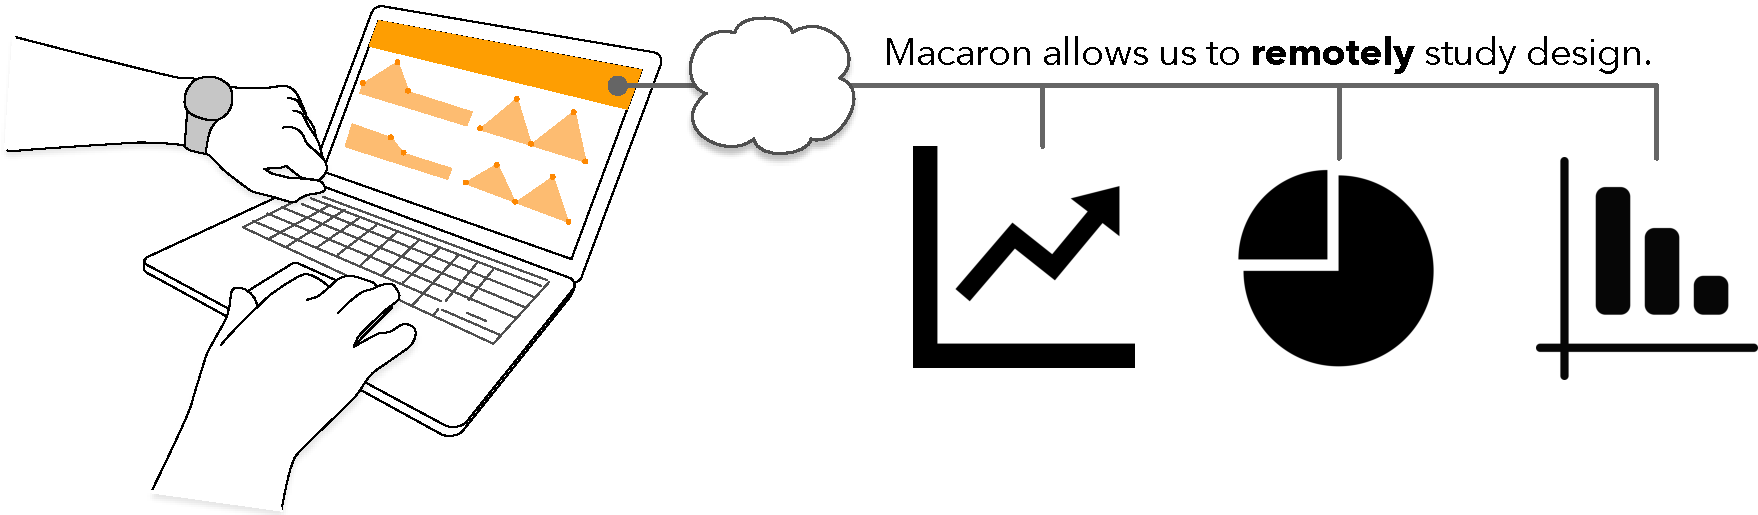
\includegraphics[width=0.9\textwidth]{poster/MacaronPoster-HS16-conceptsketch-words}
\caption{Concept sketch for a Macaron, an online, open-source VT editor features incorporable examples and remote analytics.}
\label{hapticexamples:designgallerysketch}
\end{center}
\end{figure}

In both the Haptic Instrument and Tactile Animation case studies, participants drew from their experience or external examples and requested features for repetition.
%This is unsurprising; creative tasks, like design, are often defined as the recombination of existing ideas, with a twist of novelty or spark of innovation by the individual creator \cite{Warr2005}.
Because we explored haptic design tool implementation and rendering pipeline in-depth in \autoref{ch:tactileanimation}, with Project Macaron\footnote{Published and demoed at Haptics Symposium \cite{Schneider2016macaron}.} we instead move the focus to capturing more of the design process, with example-use as the target phenomenon.
Creativity often sparks when an inventor, examining existing ideas, sees a way to combine them with a novel twist~\cite{Warr2005}.
% Creativity often sparks when the inventor sees a way to combine existing ideas with a novel twist~\cite{Warr2005}.
An environment rich with \emph{examples} is fuel for this fire. In industrial and graphic design \cite{Buxton2007,Herring2009} their use improves process and final results~\cite{Dow2011,Lee2010a}.
%Examples are critical to provide inspiration, guidance, and inform design \cite{Herring2009,Buxton2007}; for example,
%%In other fields of design, designers clip, store, and display examples for inspiration \cite{Buxton2007}.
%industrial designers collect various knobs and materials, and web designers bookmark sites \cite{Herring2009}.
%Managing these examples effectively is already a significant task even in these more visual fields, but there is no explicit support for vibrotactile (VT) design.
%I will investigate interaction techniques to directly use examples in haptic design through a design gallery tool for VT icons (\autoref{hapticexamples:designgallerysketch}).
Design galleries are used in graphics and web design to facilitate the use of examples \cite{Lee2010a,Marks1997}.
While there are several challenges involved with examples in design, including capture, search, management, use, and sharing, I limit this project's scope to the \emph{combining} existing examples to create new VT icons.

Problem preparation -- also known as the ``problem setting" \cite{Schon1982} or ``analysis of problem"~\cite{Warr2005}
%\osC{or ``collect"~\cite{Shneiderman2000}} 
step of design -- involves 
% getting a handle on the problem 
immersion in the challenge
and drawing inspiration from previous work. %, and and establishing a first general approach with which to attempt a solution.
%Sch\"{o}n demonstrated that designers initially frame their problems before developing a solution \cite{Schon1982}.
%Sch\"{o}n also describes the designer's repertoire, their collected experience, which aids in design.
Both may come from the designer's experience,  \emph{repertoire}~\cite{Schon1982} or exposure to a symbolic domain, e.g., mathematical theorems and notation %, or techniques for painting
\cite{Csikszentmihalyi1996}.

To this end, external examples are critical in inspiring, guiding and informing design \cite{Herring2009,Buxton2007}. 
Industrial designers collect objects %various knobs
and materials; web designers bookmark sites \cite{Herring2009}.
In graphics and web design, \emph{design galleries} organize examples to be  immediately at hand % in the design process
~\cite{Lee2010a,Marks1997}.
% \emph{Design galleries}  are used in graphics and web design to include examples immediately at hand in the design process~\cite{Lee2010a,Marks1997}.
Example-based tools often use sophisticated techniques to mix and match styles and content~\cite{Kumar2011}: this requires immediate access to the examples' underlying structure.

Several effect libraries are available to designers of vibrotactile (VT) sensations, e.g., for accessible wayfinding \cite{Zelek2003} or % rich 
media experiences \cite{SchneiderAsiaHaptics2014,Israr2014,ImmersionCorporation,Culbertson2014}. 
%\kmC{slc} % leave out Seifi2015? since it does not have all these limitations. use as positive example instead?
But despite the need for effect customizability~\cite{Seifi2014}, VT library elements are generally opaque in construction and immutable.
Recent advances include limited parameter adjustability~\cite{Israr2014,SchneiderAsiaHaptics2014} and faceted library search and browsing~\cite{Seifi2015}. 
Despite this, designers still must either choose a pre-existing sensation or build from scratch:
\textit{elements cannot be sampled, recombined, built upon or adapted}. %imitated with variations.
In contrast, web designers can access a page's source;
graphic and sound designers can sample and incorporate colours and sounds from other media.



\begin{figure}
        \centering
%        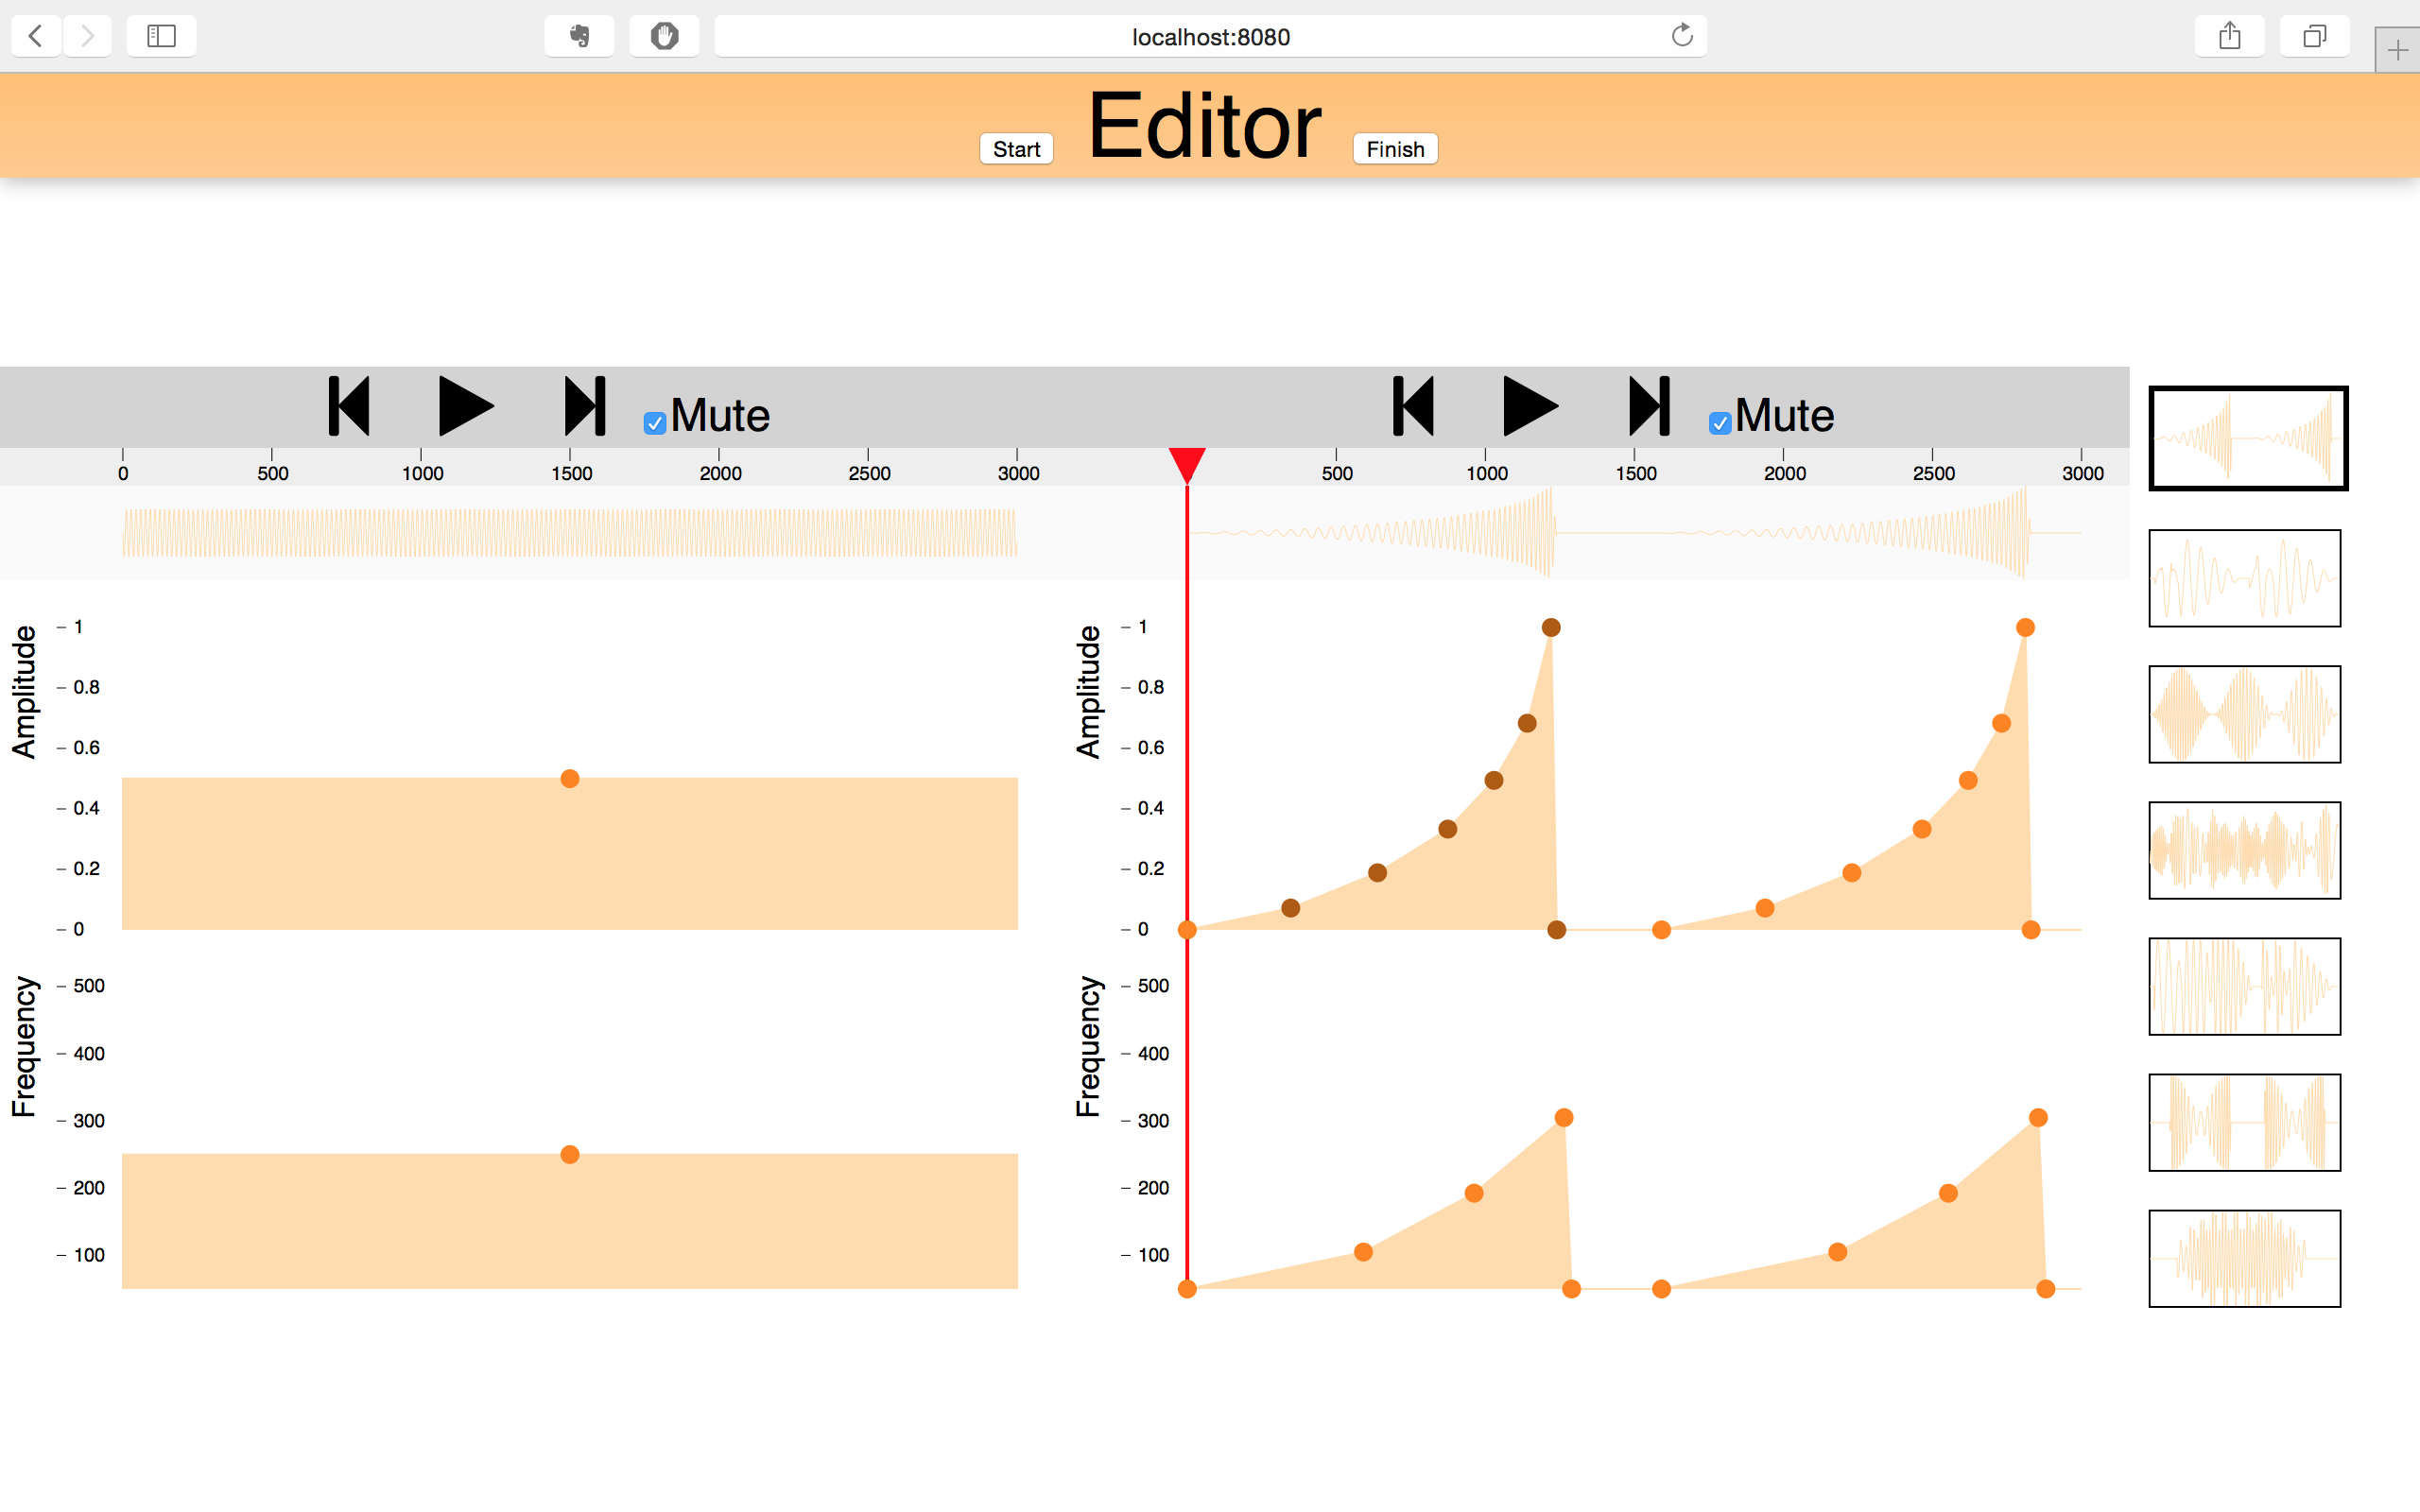
\includegraphics[width=0.8\textwidth]{full/MacaronScreenshotHi}
        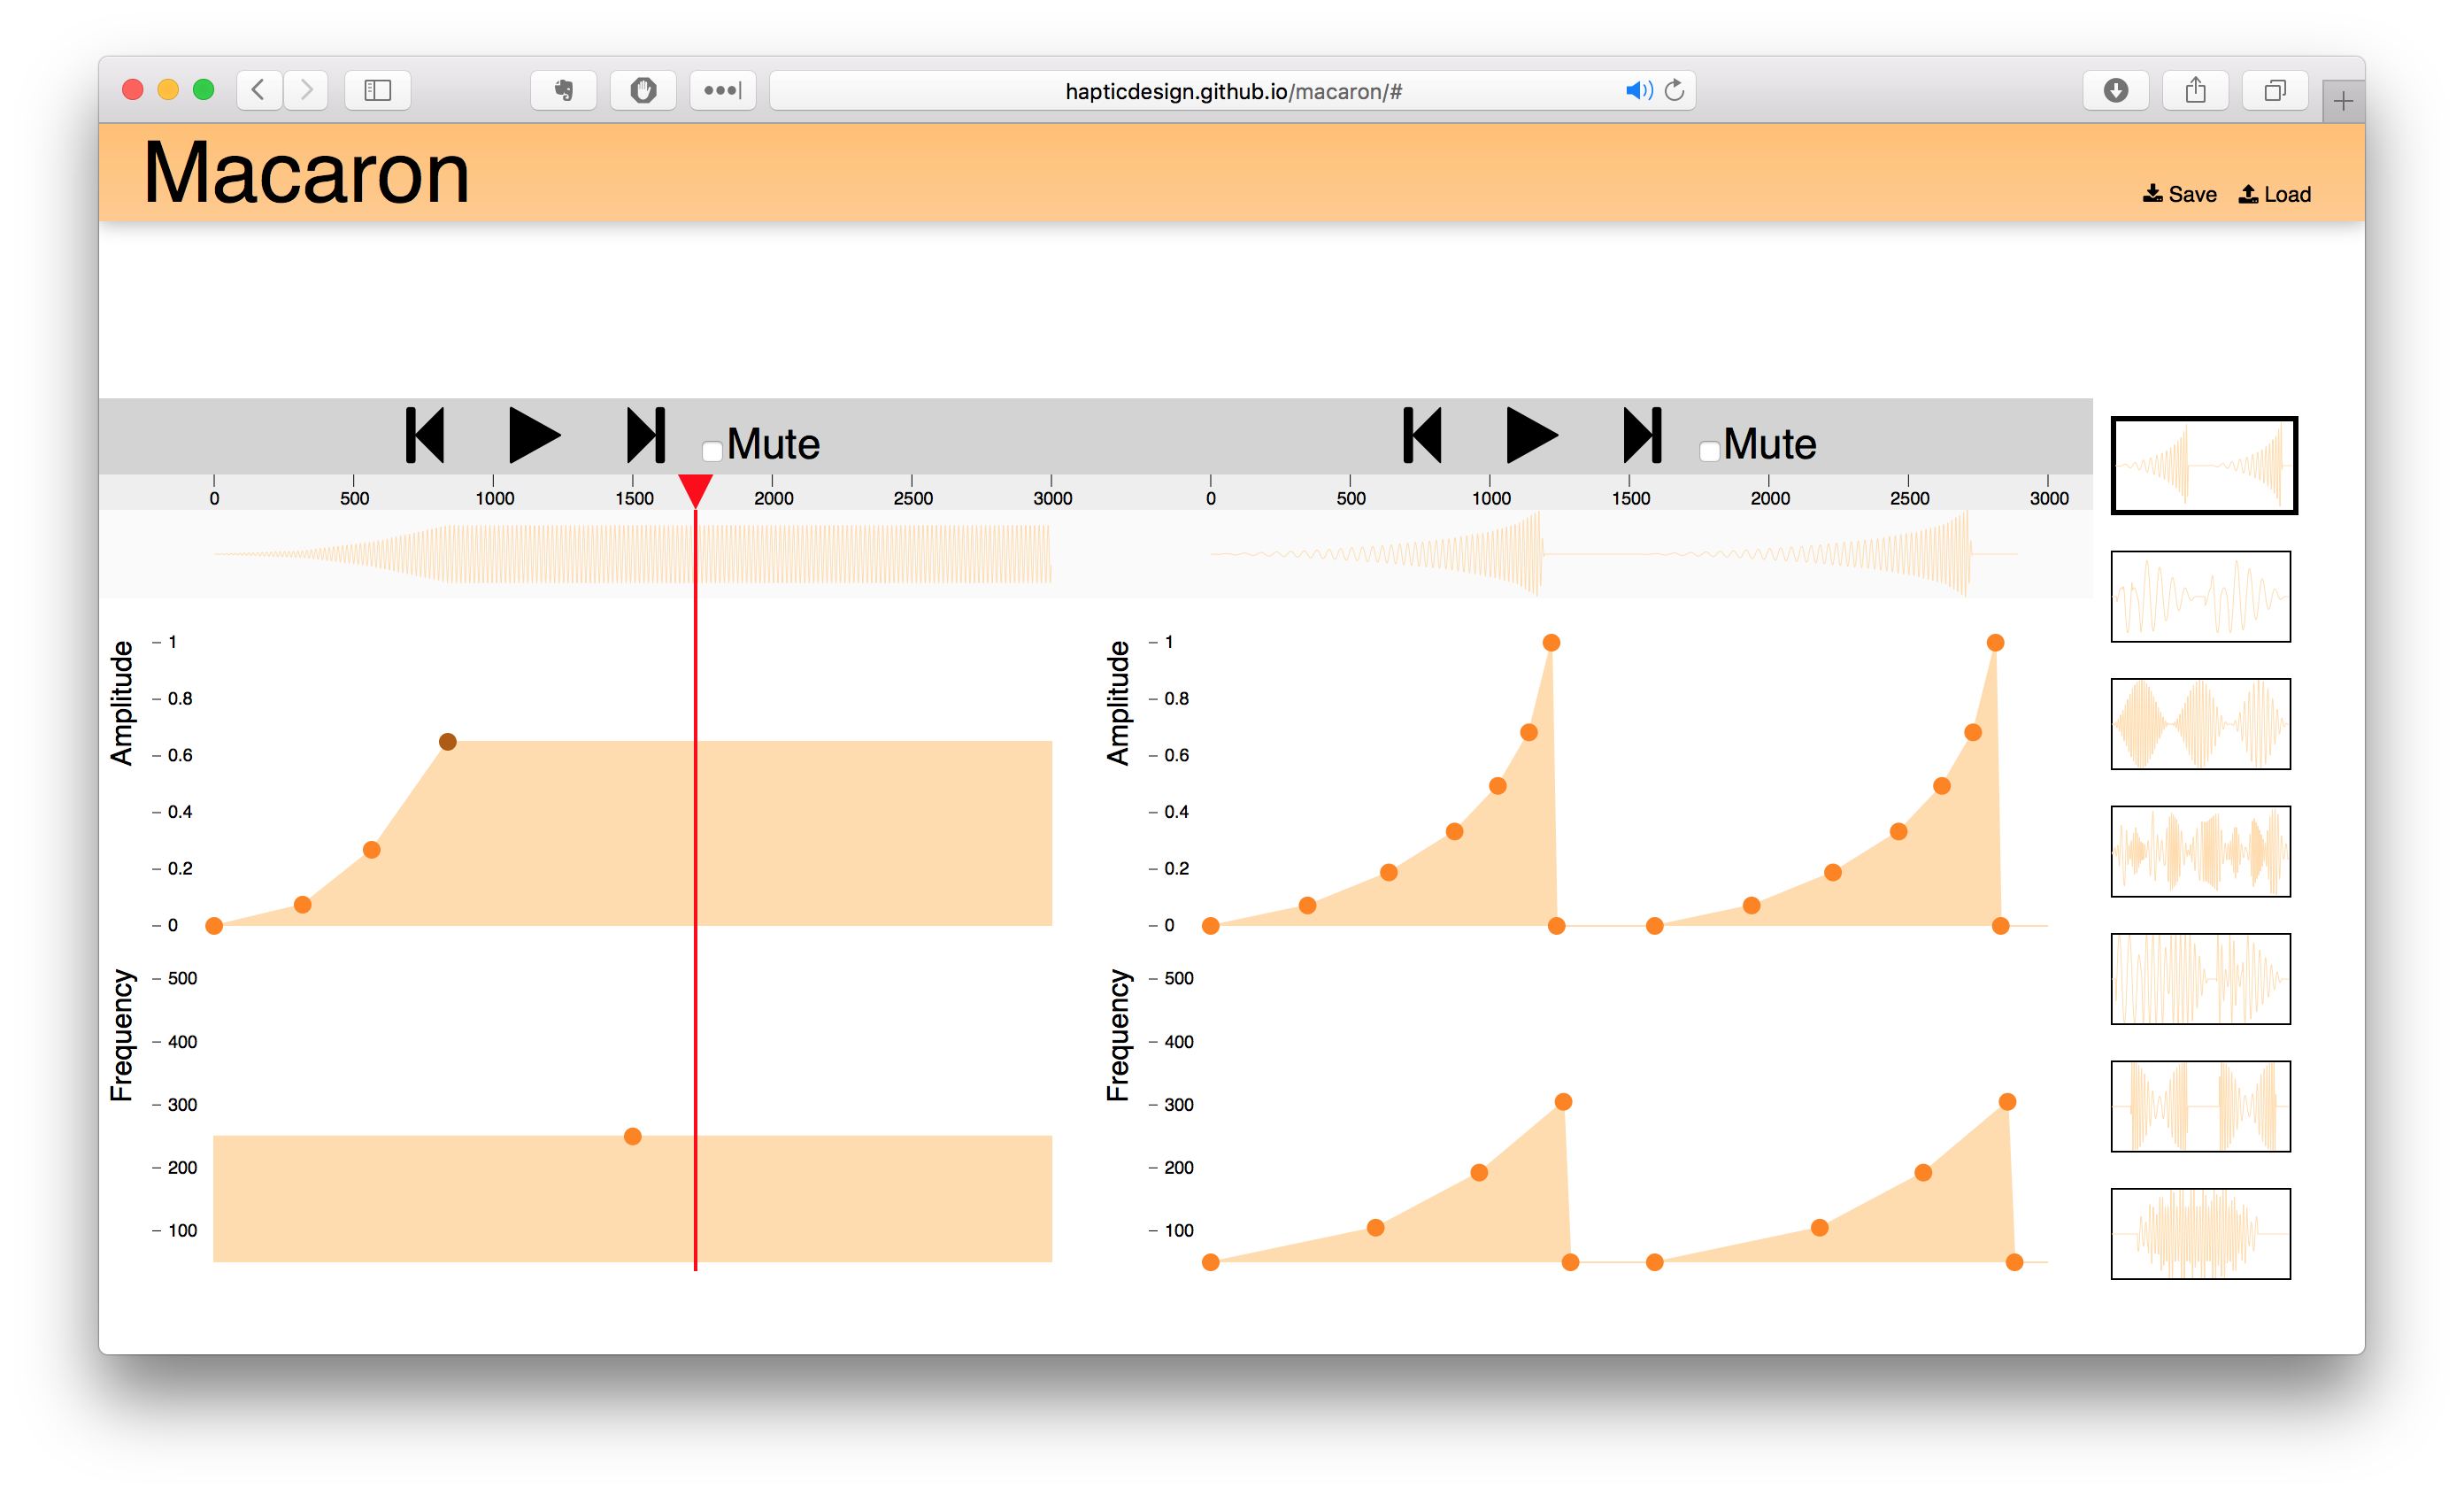
\includegraphics[width=0.9\textwidth]{poster/IMG-MacaronScreenshot-Poster}
        \caption{Macaron interface, ``\hi'' version featuring both composability (copy and paste), and visibility of underlying parameters. The user edits her sensation on the left, while examples are selected and shown on the right. 
%        One editor has focus at a time, shown by the red playhead. Examples are non-modifiable (keyframes cannot be inserted or moved).
        Macaron is publicly available at \emph{{\tt hapticdesign.github.io/macaron}}.
}
        \label{fig:macaron:hi}
\end{figure}


Here, we \textit{examine the potential role of examples} in VT design, to establish how to best support their use.
% Here, we examine the role of examples in VT design.
We designed a web-based editor and interactive \emph{design gallery} \cite{Lee2010a,Marks1997} (\autoref{fig:macaron:hi}) for VT sensations,
then asked users to compare versions (\autoref{fig:versions}) that vary in example accessibility via \emph{visibility} and \emph{incorporability}, as they create VT effects for animations (\autoref{fig:animation}).
%\kmC{adequate grounding of this choice? slc} % KM 11.07 1227 as I come back later to these terms (in tool variant choice, then results) I realized there is not a lot of justification for choosing these dimensions. I think we had really good reasons for going this way, but it doesn't come across.

%We then compare versions of this tool which vary in power of examples use: the editor alone, relative to designer access to examples with low or high \emph{visibility} and low or high \emph{composability}.
Analysis of user action logs provide an objective picture of the VT design process. To validate the deployment of this methodology at scale, we also interpret and validate logs with direct observation and interviews.
%Specifically, we:
%\begin{itemize}
%\item introduce \textit{Macaron}, a web-based VT effect editor through which examples can be used directly in designs,
%\item find that \textit{visible, incorporable examples make design easier} by providing a starting point for design and scaffolding to learn how to work with VT parameters,
%\item identify \textit{implications for future tools and libraries}, and
%\item discuss the \textit{opportunities afforded by a web-based editor} as a practical tool and platform for studying other aspects of VT design at scale.
%\end{itemize}









\newcommand{\macaronBigImageWidth}{0.55\textwidth}
\newcommand{\macaronSmallImageContainerWidth}{0.42\textwidth}
\newcommand{\macaronSmallImageWidth}{0.24\textwidth}


% \begin{figure*}[htb]
% % \centering
%     \centering
%         \begin{subfigure}{\macaronSmallImageWidth}
%             % \centering
%             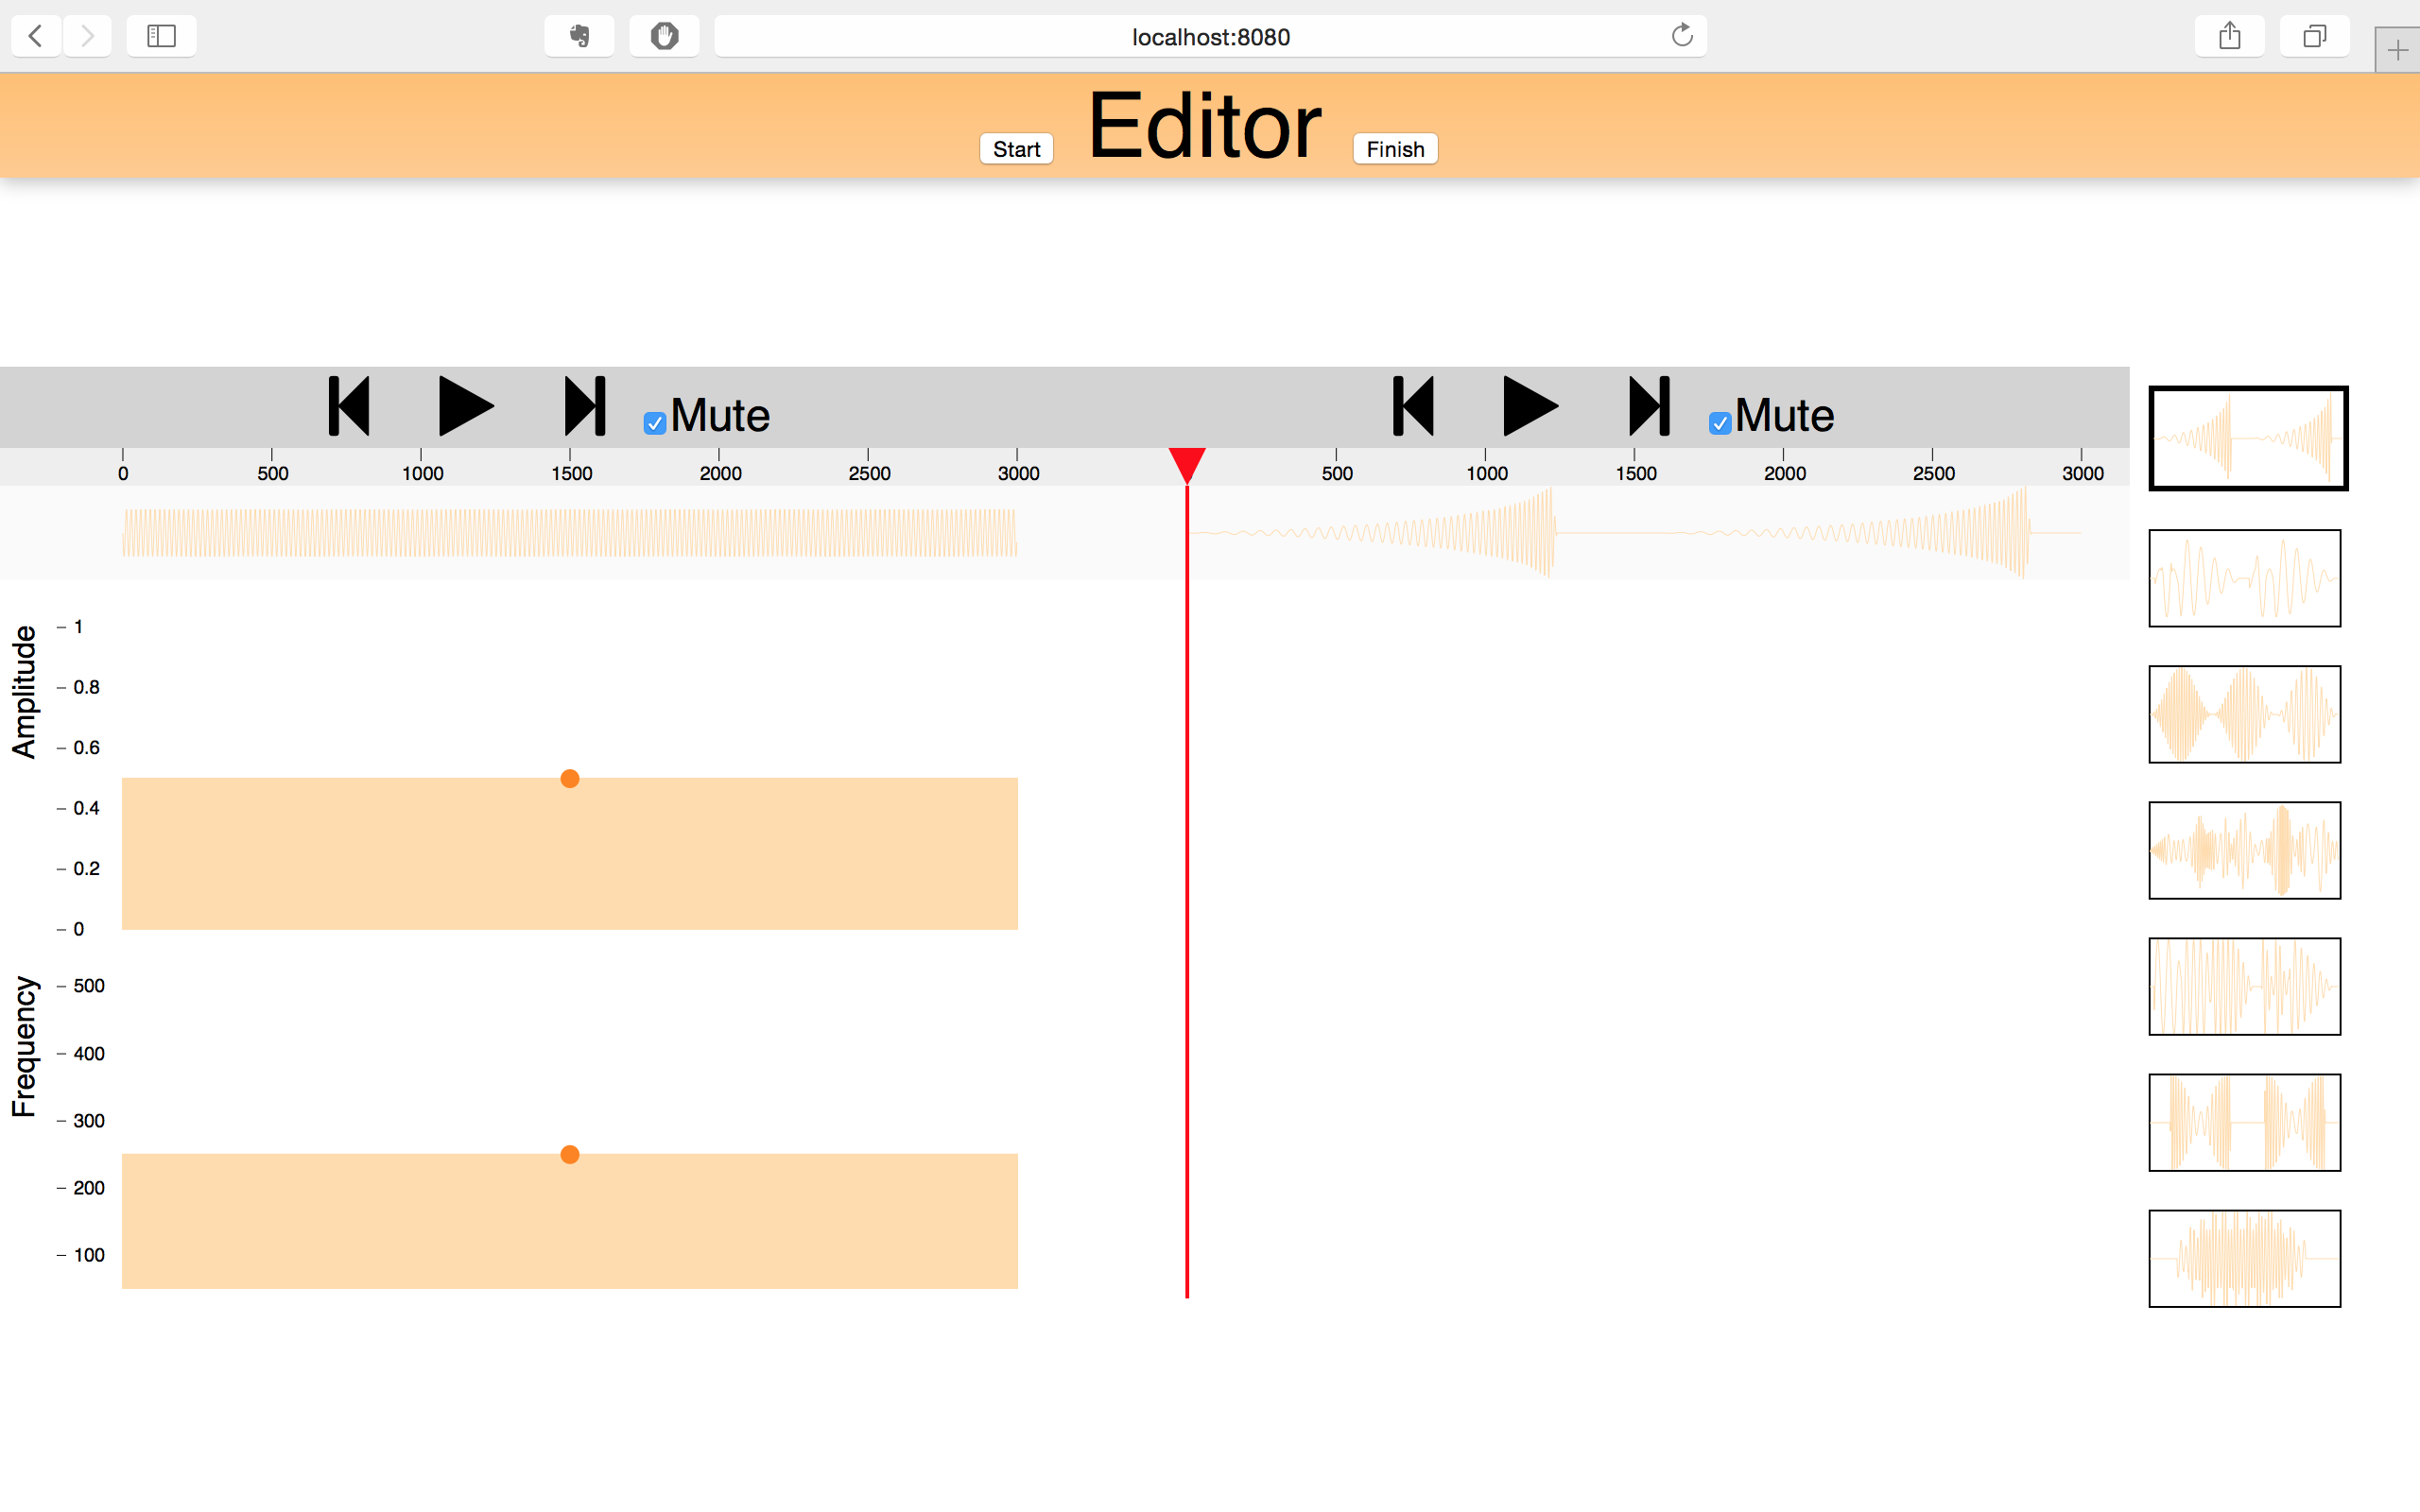
\includegraphics[width=\textwidth]{MacaronScreenshotLo}
%     	   \caption{\lo version.}
%     	   \label{fig:macaron:lo}
%         \end{subfigure}
%         \begin{subfigure}{\macaronSmallImageWidth}
%             % \centering
%             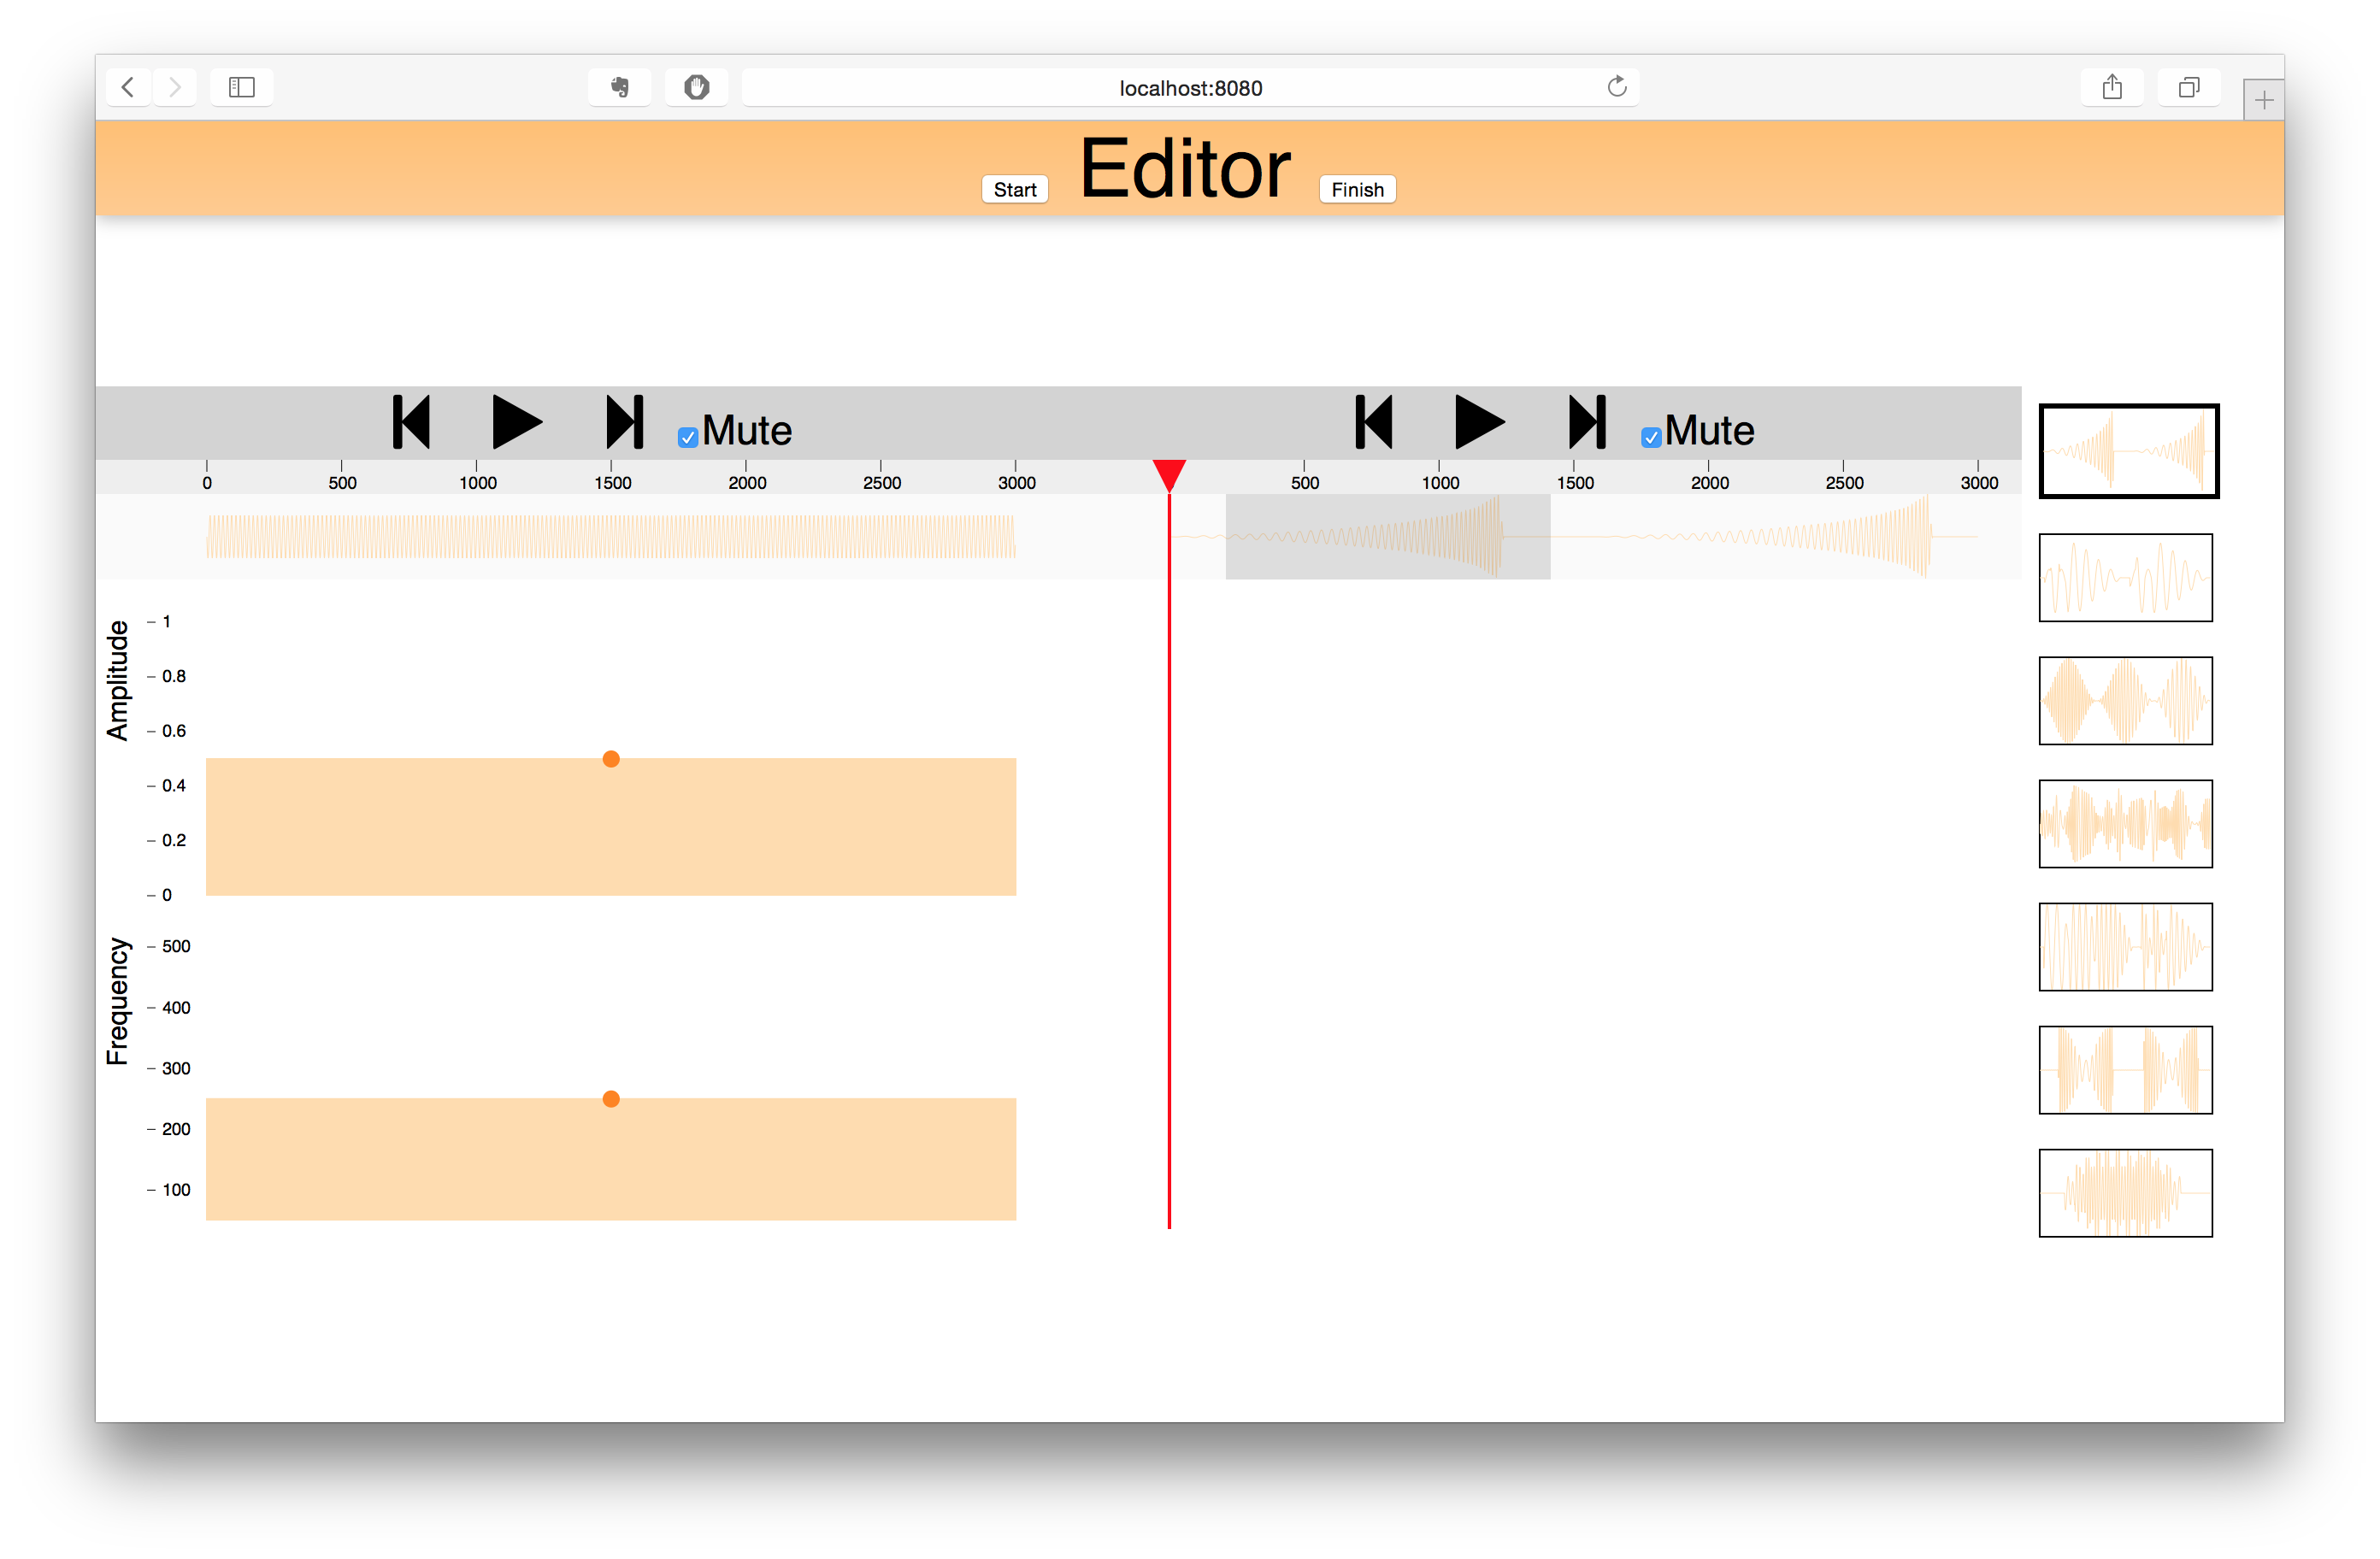
\includegraphics[width=\textwidth]{MacaronScreenshotSelect}
%     	   \caption{\select version.}
%     	   \label{fig:macaron:select}
%         \end{subfigure}
%         \begin{subfigure}{\macaronSmallImageWidth}
%             % \centering
%             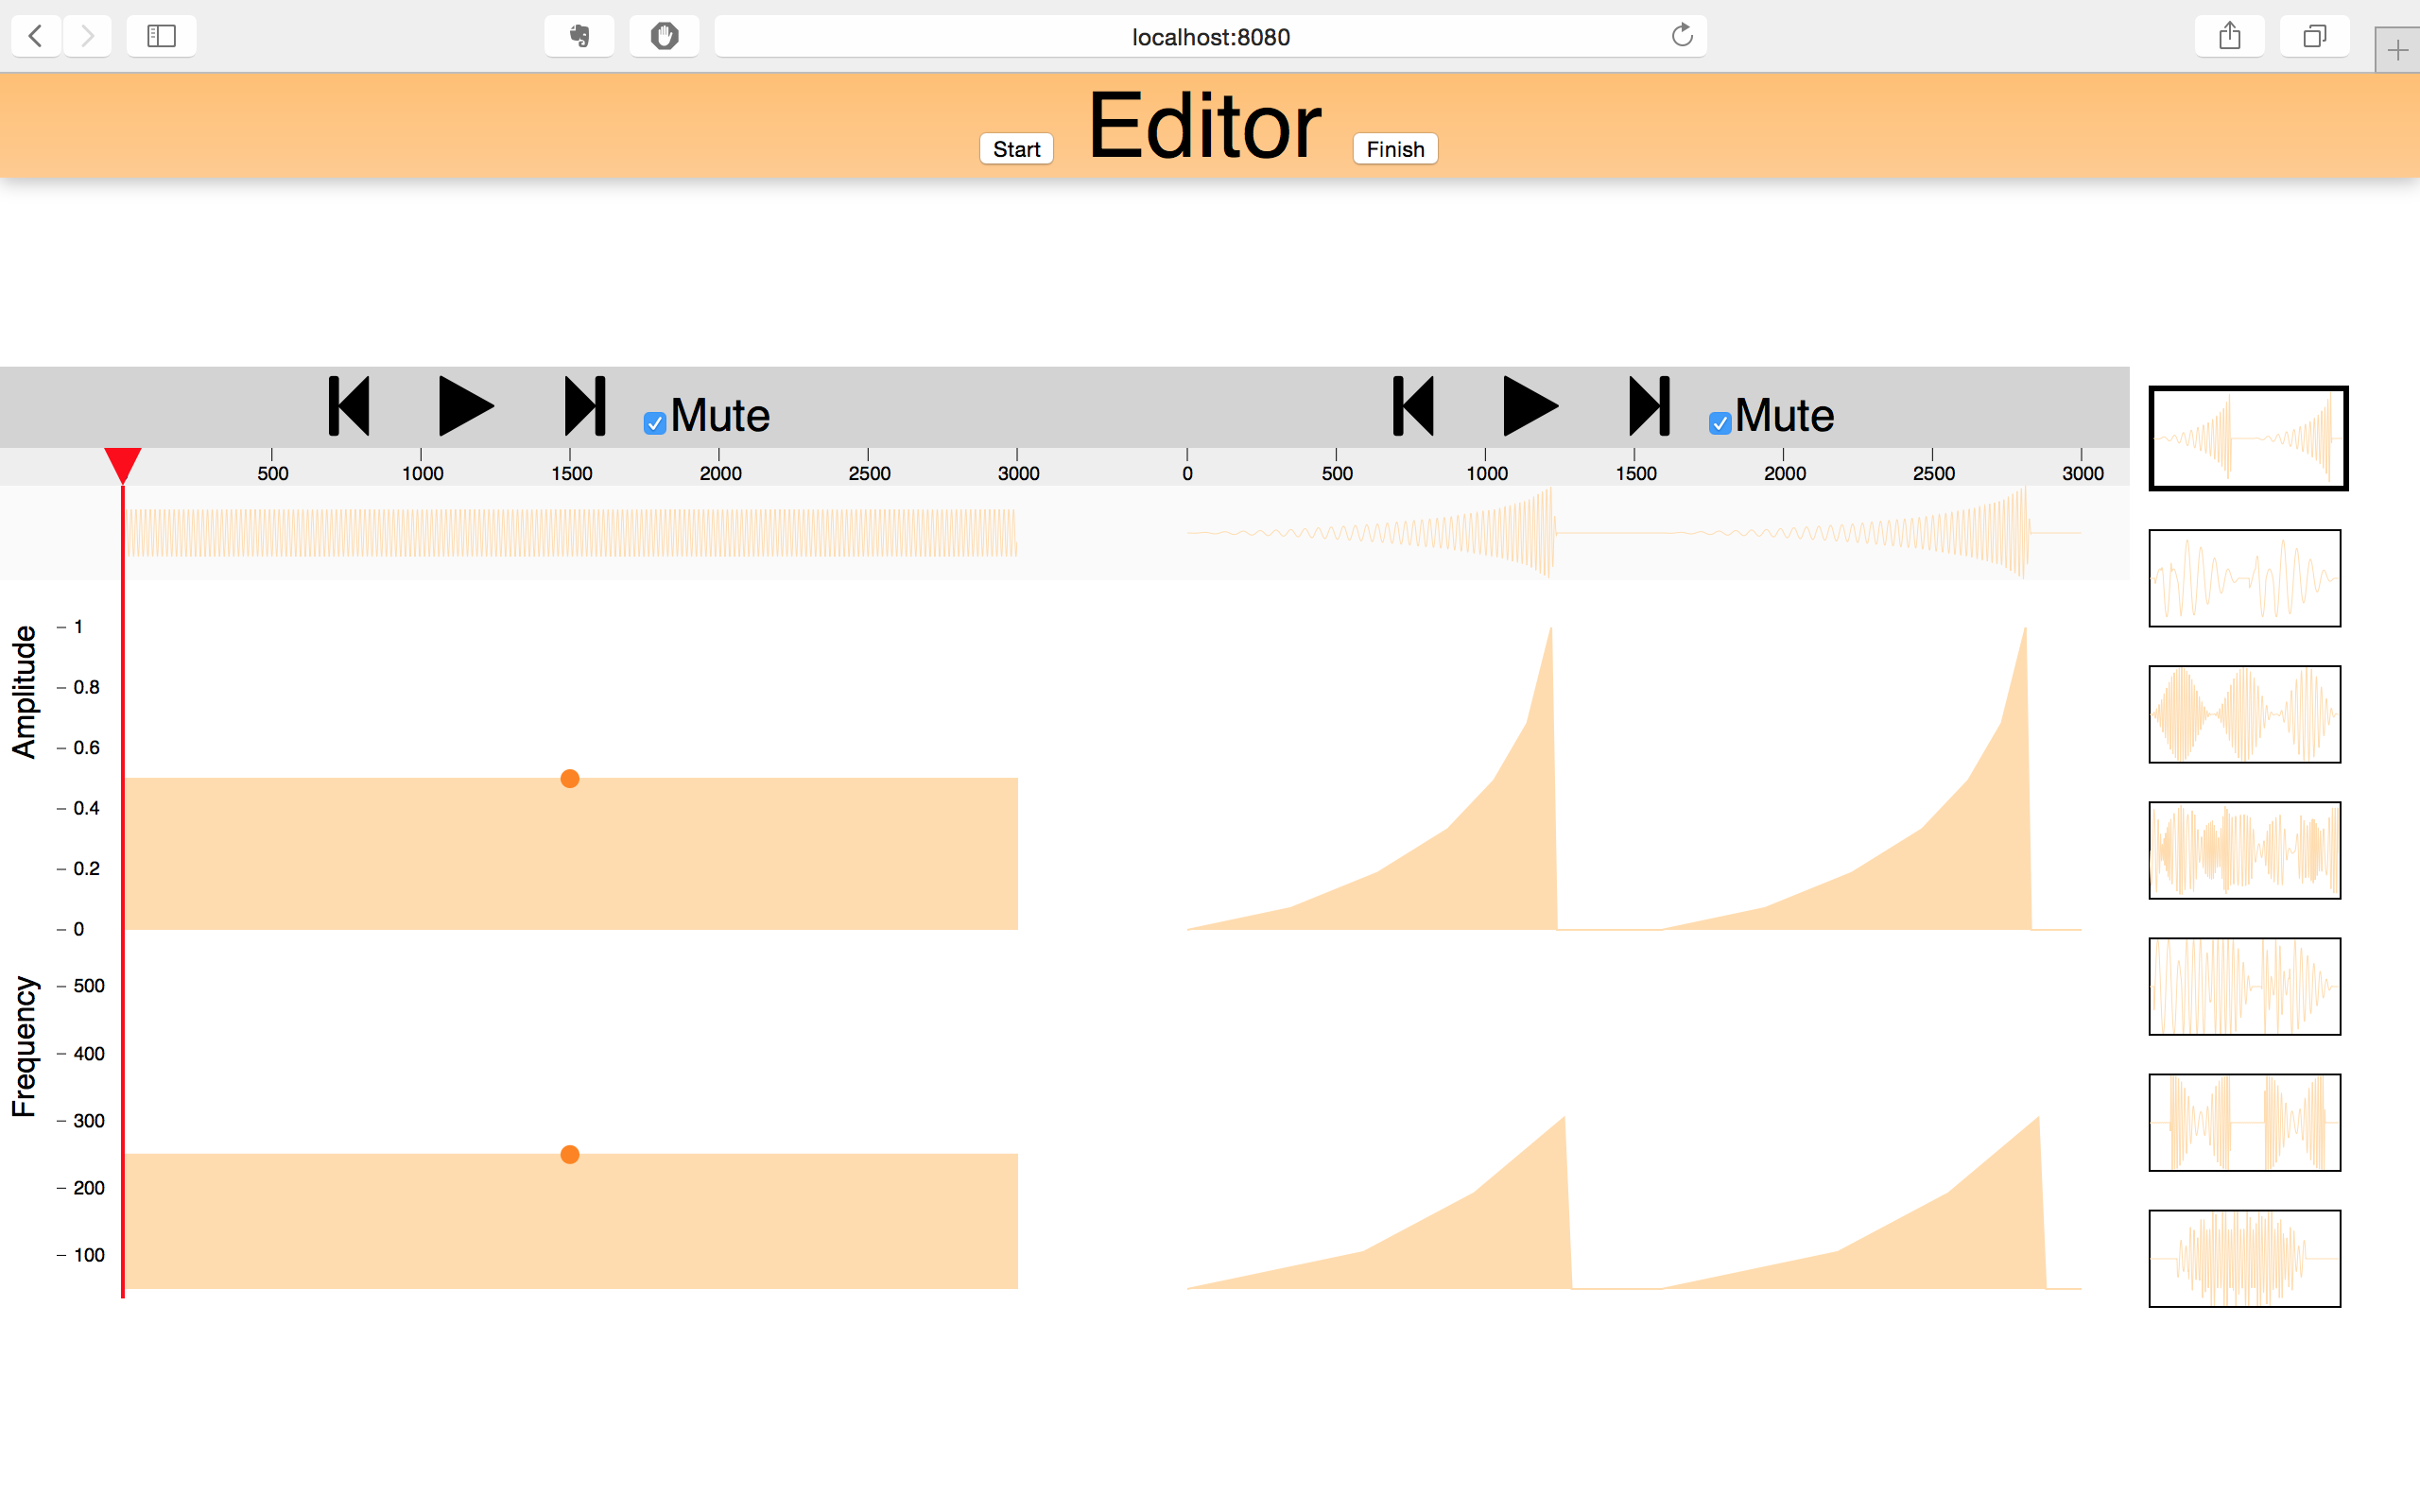
\includegraphics[width=\textwidth]{MacaronScreenshotVis}
%     	   \caption{\vis version.}
%     	   \label{fig:macaron:vis}
%         \end{subfigure}
%         \begin{subfigure}{\macaronSmallImageWidth}
%             % \centering
%             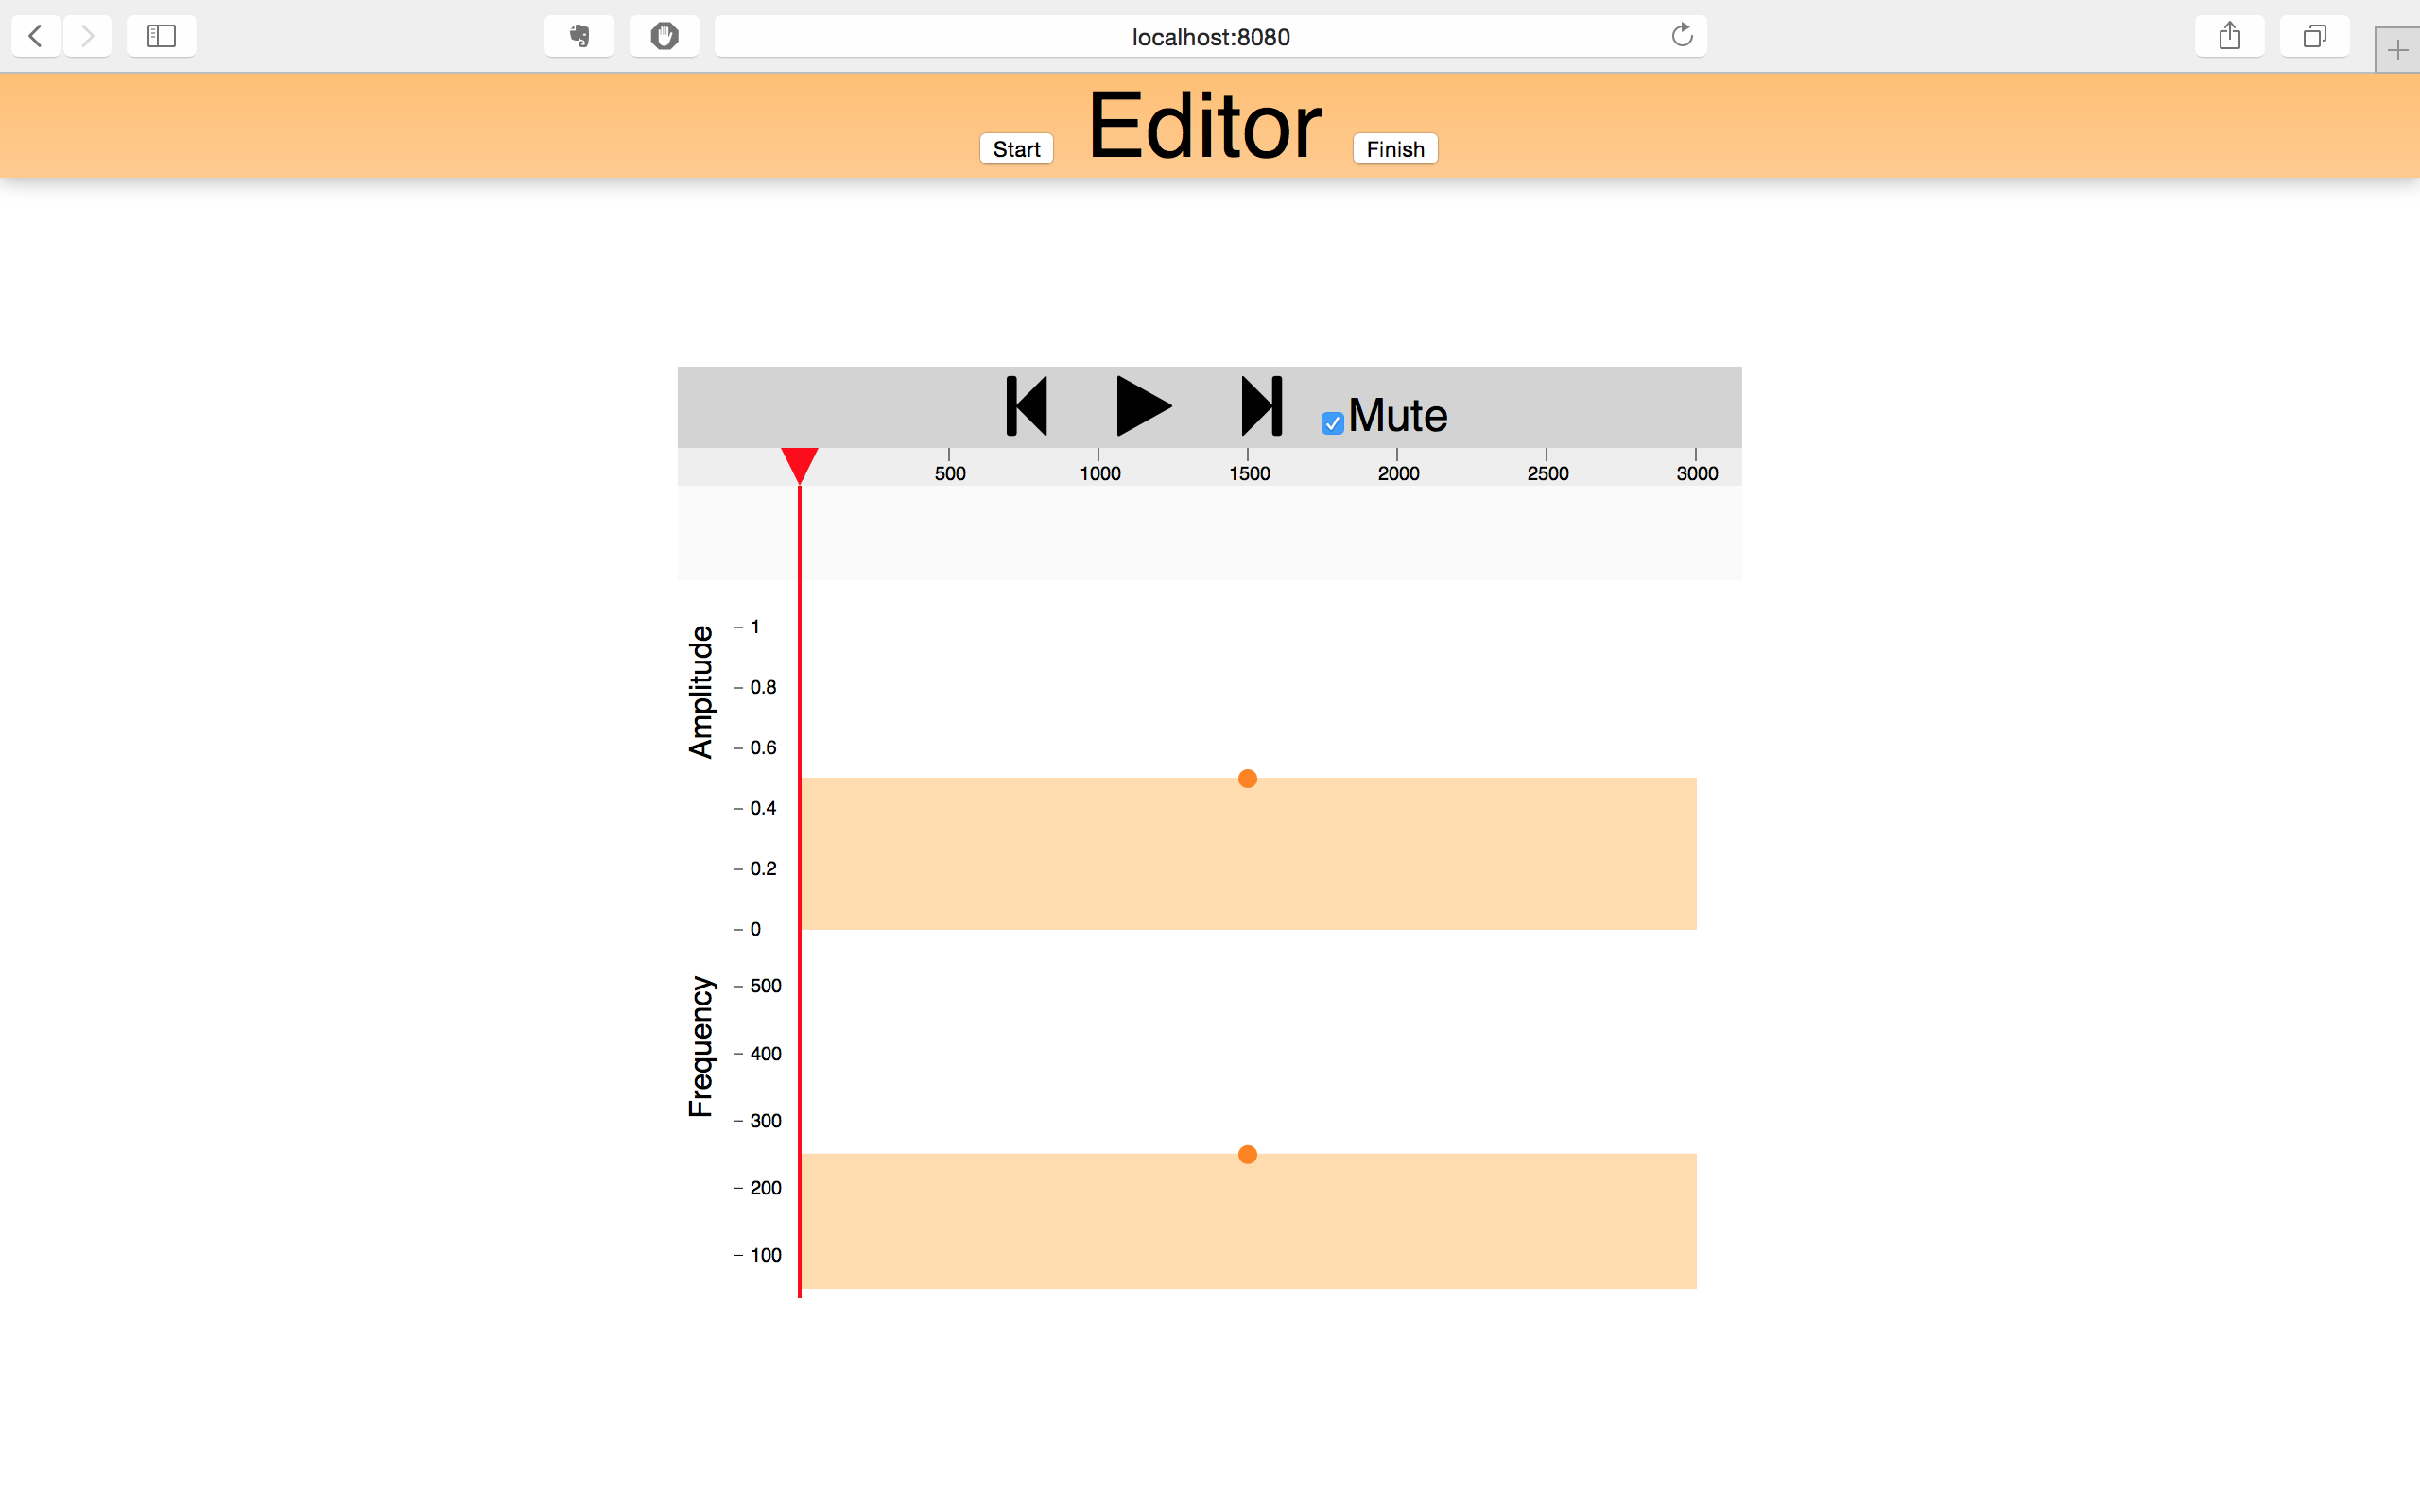
\includegraphics[width=\textwidth]{MacaronScreenshotNone}
%     	   \caption{\none version.}
%     	   \label{fig:macaron:none}
%         \end{subfigure}
    
%     \caption{Alternative Macaron interfaces. \lo has examples that can be felt, but only the waveform is visible (simulating the status quo for libraries). \select shows the vibration, and allows selection and copying from the waveform visualization. \vis is the opposite: showing the underlying vibrations, but with no selection or copying. \none has no examples at all.}
%     \label{fig:macaron}
% \end{figure*}


%%%%%%%%%%%%%%%%%%%%%
%
% SECTION: Related work
%
%%%%%%%%%%%%%%%%%%%%%
%\section{Related Work}
%% Previous work includes VT effects, past approaches to VT design, and example use in non-haptic design.
%
%%%%%%%%%%%%%%%%%%%%%%%%
%\subsection{Salient factors in VT effect perception and control}
%% Haptic icons  have long been an important tool for structuring vibrotactile design, typically manipulated with amplitude, frequency and waveform~\cite{Gunther2002,MacLean2003,Brewster2004,maclean2008foundations}.
%Vibrotactile effects (e.g. haptic icons~\cite{MacLean2003}) are typically manipulated with low-level engineering of signal parameters, beginning with  amplitude, frequency and waveform~\cite{Gunther2002,MacLean2003,Brewster2004,maclean2008foundations}.
%%
%%Different granularities of amplitude and frequency control show that
%Rhythm can support large, learnable icon sets \cite{Ternes2008,Swerdfeger2009a};  combining waveforms enhances roughness \cite{GunhyukPark2011}.
%Time-varying amplitude adds musical expressivity, from tactile crescendos \cite{Brown2006} to 
%%attack-decay-sustain-release (ADSR)
%envelopes \cite{Schneider2014}.
%Multi-dimensional scaling % (MDS)
%can be used to identify %, confirm, 
%and elaborate these parameters \cite{MacLean2003,VanErp2003,Enriquez2006,Hollins2000}.
%
%Affect and metaphor are another way to structure and manipulate sensations at a level more cognitively relevant than engineering parameters.
%Perceived valence (pleasantness) and arousal can be influenced by  frequency/amplitude combination \cite{YongjaeYoo2015,Obrist2015}.
%Metaphors \cite{chan2008,Obrist2013,Seifi2015} and use cases \cite{chan2008,Seifi2015} offer structure, memorability and design language.
%% While we focus here on single-actuator displays, 
%Spatial displays require additional controls for location and direction, % for users to work with, 
%whether body-scale \cite{Gunther2002,Israr2011a}, mobile  \cite{Seo2013}, or mid-air \cite{Obrist2015}.
%While many parameters are available for VT design, we chose the most established (time-varying frequency and amplitude) for Macaron's initial implementation.
%%Location and direction also influence affective perception \cite{Obrist2015}.
%%\kmC{summarize? slc} % KM 11.07 1143 this section needs a brief capture statement. My rework of ss heading helps, but problem is,  you've listed a ton of parameters, but not said how this relates to Macaron. This would be a place to say "we chose the three most basic ones to start exploring these ideas (freq, amp, time invariance), but clearly there's a lot of headroom to bring in other manipulables in the future?
%
%%\begin{itemize}
%
%%\item (briefly) what parameters today's technology gives control discretion over, and the scale at which these play out (temporal granularity? thinking about difference between amplitude and rhythm). Mention technology insofar as to say ``this is what the tech requires you to control; and this is what people perceive as perceptual dimensions that thus should be controlled''.
%
%%\item what parameters have been found to have expressive benefit (rhythm wins, waveform loses). Emotional parameters (Sri, Seifi)
%
%
%%\item what expressive control entails. Focus here on the stimulus properties and their perception, not the tools used to draw them out.
%
%%\item while design space is certainly more limited than visual and auditory design, a considerable and expressive freedom exists (e.g. Ternes, Swerdfeger thesis - pretty large sets are learnable). 
%
%%\osC{missing some synthesis, slc} %KM: I haven't been able to fully process or express what you've suggested here
%%\item what makes it hard to access the expressivity that does exist is: 
%%(a) serial nature that can be hard for an editor to represent in overview and in comparison with alternatives (a challenge faced by other temporal-media editors) 
%%(b) poor predictability of how superposed dimensions (e.g. tracks) will interact perceptually (?)
%%(c) big problem: machine parameters aren't necessarily the right perceptual parameters [but, this isn't quite the one you're going after here] 
%
%%(d) ``blank sheet'' problem - perennially needing to start from scratch - identify as the one you're focusing on here.
%
%
%%\end{itemize}
%
%
%%\noindent Fodder: 
%
%%- Amplitude and frequency are identified as the primary low-level design parameters for single-location VT actuators \cite{Gunther2002,Schneider2014}.
% 
% %- rhythm and other time-invariant patterns occur at a different scale; perceptually extremely important -  Mention van Erp 2003, Brown 2006, Ternes 2008
%
%%- Waveform less expressive \cite{Gunther2002}.
%
%%%%%%%%%%%%%%%%%%%%%%%%
%\subsection{Past approaches to VT design}
%% Several tools have been built to aid VT design.
%Past editors -- e.g., the Hapticon Editor \cite{Enriquez2003}, Haptic Icon Prototyper \cite{Swindells2006}, posVibEditor \cite{Ryu2008}, Vivitouch Studio \cite{Swindells2014}, and Haptic Studio (www.immersion.com) -- are track-based, with graphical representations to edit either waveforms or profiles of dynamic parameters.
%Additional features (e.g., spatial control or mobile interfaces) are surveyed in \cite{Schneider2015}.
%%Features include the combination or multi-tracking of effects, utilizing a library of existing effects, and the ability to play back sensations.
%
%A library of effects is critical for haptic design tools \cite{Schneider2015}. Most existing tools support feature saving/loading, and some have an internal component library \cite{Enriquez2003,Swindells2006,Swindells2014}.
%However, previous implementations were primarily \emph{compositional}, employing building blocks~\cite{Enriquez2006} %that can be combined to create more complex sensations \cite{Enriquez2006}.
%rather than complete artifacts. Example use was not studied.
%%In Macaron, we also investigate examples of full, created and complete artifacts, built right into the tool.
%%\kmC{careful/confused slc} 
%% in this par you seem to be saying existing libraries only have bits, not full things. [caution: Swindells examples allowed for examples to be complete as well as partial. I'd back off on this.]
%% in next par, you seem to say the opposite: libraries only have whole examples, you can't pick and choose from internals. 
%
%%This  \kmC{what is??} is more analogous to 
%% Complete artifacts are found in large libraries of VT icons, but with limitations.
%Large VT libraries contain complete artifacts, but impose a serious constraint on their use.
%In the Immersion Touch Effects Studio library,
%% of tactile icons supplied on a mobile platform, but 
%underlying structure and design parameters are hidden and cannot be incorporated into new designs. %, and examples cannot be incorporated into a new project.
%VibViz \cite{Seifi2015} features 120 VT examples with visualizations searchable by several taxonomies, but the selection model is all-or-nothing.
%FeelCraft \cite{SchneiderAsiaHaptics2014} proposes a community-driven library of feel effects \cite{Israr2014} for simple parametric customization and re-use. %\kmC{and?} % how does Feelcraft fit in here? are you talking about FC in next sentence? if so, need to connect end-user customization better to FC.
%While end user customization-by-selection is important \cite{Seifi2014},  
%experts need a more open, editable model,
%% we suggest a more open model for experts. %this \kmC{what?} still represents a library of selectable, all-or-nothing designs.
%%Compare this to
%% For example, web designers can view source code at any time, with recent tools allowing search and easy incorporation of elements
%just as web designers rely on full access to source code with recent tools allowing search and easy incorporation % of elements
%% interactive \emph{design galleries} allow users to search and incorporate elements from other sites 
%\cite{Lee2010a}.
%% search sites to see what others are doing \cite{Lee2010a}.
%%\kmC{Needs summary sentence to close slc} % KM 11.07 1140 this section needs a focus - I'm uncertain of the point being made with the cited work, they seem contradictory. In addition to comments above, suggest close with a sentence on "hole left that this work fills". 
%% ALSO, this section seems a little long >.25/6 pgs+ 8-10 refs - although it is likely most impt part of RW, consider dropping one or two cases.
%
%% \begin{itemize}
%% \item Other editors have had some success in going after "what makes VT design hard''. They've introduced track-based design, exposed underlying parameters, helped with rapid prototyping, visualization, and sharing of sensations. They vary in the degree to which they support``choosing'' vs ``modifying'' (use Seifi terminology) and how they expose innards. 
%
%% \item Past use of examples goes this far: Swindells allows things to be saved and re-used (but not sampled, and only used in narrow ways), VibViz allows library browsing but doesn't show underlying construction (well, a bit). Immersion editor...
%
%% \item Here, we aren't so much introducing new features or abilities, but we want to turn the knob on the ``example'' thing to see how it actually impacts the design process.  [i.e., don't claim that Macaron is first to employ examples. But do say that it is novel to study it in a variable way]
%
%% \end{itemize}


%%%%%%%%%%%%%%%%%%%%%%%
%\subsection{Examples in non-haptic design}
%% [actually, suggest leaving this out. Already said in 1st para.] Innovative recombination of existing ideas is at the heart of many design inventions~\cite{Warr2005}, and is spurred by immersion in an example-rich environment \kmC{REF?}.
%%Creative tasks, like design, are often defined as the recombination of existing ideas, with a twist of novelty or spark of innovation by the individual creator \cite{Warr2005}.
%
%Problem preparation -- also known as the ``problem setting" \cite{Schon1982} or ``analysis of problem"~\cite{Warr2005}
%%\osC{or ``collect"~\cite{Shneiderman2000}} 
%step of design -- involves 
%% getting a handle on the problem 
%immersion in the challenge
%and drawing inspiration from previous work. %, and and establishing a first general approach with which to attempt a solution.
%%Sch\"{o}n demonstrated that designers initially frame their problems before developing a solution \cite{Schon1982}.
%%Sch\"{o}n also describes the designer's repertoire, their collected experience, which aids in design.
%Both may come from the designer's experience,  \emph{repertoire}~\cite{Schon1982} or exposure to a symbolic domain, e.g., mathematical theorems and notation %, or techniques for painting
%\cite{Csikszentmihalyi1996}.
%
%To this end, external examples are critical in inspiring, guiding and informing design \cite{Herring2009,Buxton2007}. 
%Industrial designers collect objects %various knobs
%and materials; web designers bookmark sites \cite{Herring2009}.
%In graphics and web design, \emph{design galleries} organize examples to be  immediately at hand % in the design process
%~\cite{Lee2010a,Marks1997}.
%% \emph{Design galleries}  are used in graphics and web design to include examples immediately at hand in the design process~\cite{Lee2010a,Marks1997}.
%Example-based tools often use sophisticated techniques to mix and match styles and content~\cite{Kumar2011}: this requires immediate access to the examples' underlying structure.
%% , requiring access to examples' underlying structure.
%

%%%%%%%%%%%%%%%%%%%%%
%
% SECTION: System Design
%
%%%%%%%%%%%%%%%%%%%%%
\section{Design}
%\kmC{OS *slc*}
% KM 02.02: (1) HEADINGS. the submitted-version headings reinforce a "build system / evaluate it" contribution model that may be leading reviewers to overlook the other contributions here. Think about tweaking the names to emphasize the scientific contribution? 
% (2) NOVELTY: this first paragraph of 'system design' is very important in establishing the objectives of the system, and also its novelty. I've tried tweaking it to push forward its experiment-driven requirements. But no novelty as a tool is expressed in this para. We have to either/both of explaining that achieving the flexibility (for an experimental platform) was hard, or that something about the tool itself is novel (and hard). Otherwise, it does sound ho-hum. Obviously this includes example use (shows up in 2nd para, I'll try to work it into first), but can we express something concrete about the rest?
%

\begin{figure}[htb]
    \centering
    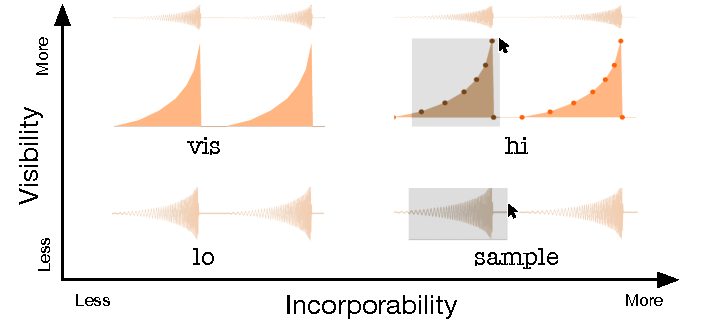
\includegraphics[width=0.75\textwidth]{VersionSpace-16-01-29}
    \caption{Design space for Macaron versions. \hi and \select both allow for selection and copying of example keyframes. \vis and \hi both show the underlying profiles. \lo represents the current status quo; only a waveform is shown.
    %\osC{slc}%"extraction/extractability"? ``sample-ability''?
    %\kmC{slc} % 11.07 10:40 I'm getting weird shadowing in this one, pretty sure it's not right. If it is, I don't understand what I'm seeing. Also it's a big figure and may not be pulling its weight.
    %OS: 02.01 I've adjusted contrast and shading issues. Does this look better?
    }
    \label{fig:versions}
\end{figure}

\begin{table}[htb]
            \small
            \centering
            \begin{tabular}{p{0.5in}p{4in}}
%            \toprule
             \textbf{\hi} & 
                  Full access to gallery examples, with keyframes visible and selectable for copy and paste.
                Simulates source visibility, \emph{e.g.}, viewing the source of a web page or having access to a {\tt .psd} PhotoShop document.
    	        \\
    	    \midrule

    	    
    	    \textbf{\select} & 
                Hides underlying parameters of frequency and amplitude, whereas waveform regions (underlying keyframes) may be copied and pasted into a design,
                simulating example mixing in absence of visibility into underlying construction.
                While possible to see underlying representation by copying the entire example, the steps are indirect and inconvenient.
             \\
    	    \midrule
    	    
    	    \textbf{\vis} & 
                Reveals underlying parameters, but hides keyframes, parameter scales, selection and copy/paste features.
                The inverse of \select, it exposes example structure, but does not support incorporating example elements into a design.
             \\
    	    \midrule
    	   
    	        	    
             \textbf{\lo} & 
                Supplies a ``black box'' outer representation. Playback and visualization of the complete vibration reflect the status quo of non-visible, non-mixable example libraries.
             \\
    	    \midrule
	    \textbf{\none} & 
                No examples present.
             \\
%             \bottomrule

    	    
            \end{tabular}
            \caption{Macaron tool alternatives, varied on dimensions of internal visibility and element incorporability.}
            \label{tab:toolAlternatives}
        \end{table}
  


To investigate VT design in the context of examples, we required a platform that would expose users' natural procedural tendencies. 
Our Macaron design gallery is simple, flexible, and extensible.
In this work, we add multiple types of example access to polished implementations of familiar concepts: \emph{tracks}, \emph{envelopes}, and \emph{keyframes}
(Figures~\ref{fig:macaron:hi},\ref{fig:versions}).
This enables easy extensions to other devices, discussed in \autoref{ch:applications}.
%
% To investigate VT design in the context of examples, we designed and built Macaron, a VT design gallery (Figures~\ref{fig:macaron:hi}-\ref{fig:macaron}).
% We built a design gallery to investigate VT design in the context of examples 
% To expose users' natural procedural tendencies, Macaron is simple, flexible, and uses familiar concepts of \emph{tracks}, \emph{envelopes}, and \emph{keyframes}. % at this early stage of development.



\emph{Tracks} are the accepted language of temporal media editors (video, audio, and past haptic efforts \cite{Swindells2006,Enriquez2003,Ryu2008}).
We provide tracks for perceptually important ``textural'' parameters (amplitude and frequency); the user accesses periodic and time-variant aspects by manipulating their 
\emph{envelopes} using
%Effects are further encapsulated as 
\emph{keyframes}, with linear interpolation in-between.
Users double-click to create a new keyframe, click or drag a box to select, and change or delete a selection by dragging or with the keyboard.
A waveform visualization reflects changes.

Macaron's example access features are inspired by more recent graphics and web design galleries \cite{Marks1997,Lee2010a,Ritchie2011}, which show examples side-by-side with the editor.
% to help ground the designer.
Other implemented features, critical for polished creative control \cite{Schneider2015}, include real-time playback, time control (scrubbing) % by the red play-bar, 
copy-and-paste, undo and redo, and muting (disables realtime VT output).
% Users can mute vibration output. 
%
To support its use as an experimental tool, user interactions are logged; 
start / stop buttons allow the user to indicate when they began and completed their design process.

 
Macaron was built with HTML5 and JavaScript, using React, Reflux, D3, and
Audiolet\footnote{\url{facebook.github.io/react}, \url{github.com/reflux}, \url{d3js.org}, \url{github.com/oampo/Audiolet}}. Real-time sound synthesis drove a C2 actuator.
To leave % the user's 
hands free for keyboard and mouse, the C2 is attached to a wristband; we simulate the design process for a wrist-worn wearable (as in \cite{Seifi2015}).


%
% Subsection: Alternative Versions
%

%\subsection{Alternative Versions}
%\kmC{descriptive version names?}
\emph{Evaluation Versions}: To study how examples impact design, we made four gallery versions by sampling two theoretical dimensions of example access:
% example visibility and incorporability (\autoref{fig:versions}).
element \emph{incorporability} and internal parameter \emph{visibility} (\autoref{fig:versions}, \autoref{tab:toolAlternatives}).
We hypothesized these would affect users' design processes, e.g., incorporable examples would encourage ``mixing and matching" of examples, visibility might provide insight.
%\kmC{OS: slc} % reads very oddly to have this results-type sentence here. Recall a discussion, can't remember reasoning. Can we drop it?
%However, these different versions revealed that our participants used these examples in a more nuanced way: as a \emph{starting point for each design}, and \emph{scaffolding for learning}.
%Our results indicated this nuanced.
%, two of which are analogous but not identical to visibility and incorporability.
%We discuss this later. %  finding not quite lining up with these dimensions.
%We theorize that the first, which opens the ``black box'' that is closed in most example libraries, will assist learning, encourage deconstruction, and promote internally intensive strategies like superposition (e.g., modifying envelopes of individual tracks as opposed to just pasting together frames sequentially). 
%Incorporability, on the other hand, should promote re-usability and efficiency, but it might not necessarily improve learning or sophisticated editing methods.

We compared these versions with each other and with a non-example version:
\none.
%
%\hi (\autoref{fig:macaron:hi}),
%\lo (\ref{fig:macaron:lo}),
%\select (\ref{fig:macaron:select}),
%\vis (\ref{fig:macaron:vis}).
%
In all versions with examples, the user can play or scrub the example, feeling it and seeing the waveform visualization.
We did not allow users to modify the examples, to avoid study workflow confounds.
To populate the gallery, we chose or adapted seven examples from~\cite{Seifi2015}, 
piloted them to confirm example variety, then regenerated keyframed versions with Macaron.
% To populate the gallery, seven examples were chosen or inspired from~\cite{Seifi2015}, piloted to confirm example variety, then keyframed versions were re-generated with Macaron.


%%%%%%%%%%%%%%%%%%%%%
%
% SECTION: Study
%
%%%%%%%%%%%%%%%%%%%%%
\section{Study Methods}
% \section{Study Method}
%\kmC{slc} % OS, I don't like my new section title much. Can you do better? I want to allude to what the study is about, to avoid natural assumption it's for tool usability.
Participants were tasked with creating a sensation to accompany five animations (\autoref{fig:animation}) -- SVGs (scalable vector graphics)  which can be played or scrubbed by the same means as navigating Macaron's time control.
We chose animation variety (concrete to abstract) and complexity to inspire non-obvious solutions without overwhelming.

Participants were first trained on \none\ with no animation,
then presented with five animation/version combinations.
As the least crucial source of variance, animations were presented in \autoref{fig:animation}'s constant order, while 
interface versions were counterbalanced in two 5x5 Latin square designs.
Thus, each participant encountered each animation and each interface version once; over all participants, each animation/version combination appeared twice,
with Latin squares balancing 1st-order carry-over effects.
This design confounds learning with animation task. 
We believe this is an acceptable tradeoff at this stage, allowing us balance interface order with a single participant session of reasonable length (1-1.5h).
% Once we understand the effect of example interfaces, we can choose a single version and examine other factors in future work.


% I come out of this feeling confused about factors and rationale.
% - explicitly state the factors you KEPT (incorporability and visibility) and the one you dropped.  
% - Why can you afford to overlook learning?
% - define what you got, for the price of the confound: be explicit about the constraint being satisfied.  there is both fitting a session into a single subject's time, and not choosing to run more subjects to keep the design iteration lightweight in proportion to the investigative stage. 

\newcommand{\animationHeight}{0.75in}
 \newcommand{\animationWidth}{0.27\textwidth}
%\newcommand{\animationWidth}{0.095\textwidth}

\begin{figure}[htb]
    \small
    \centering
    \begin{subfigure}{0.18\textwidth}
            \centering
            
\includegraphics[height=\animationHeight]{animations/MacaronHeart}
    	   \caption{Heartbeat.}
    	   \label{fig:animation:heartbeat}
    \end{subfigure}
    \begin{subfigure}{0.18\textwidth}
            \centering
            
\includegraphics[height=\animationHeight]{animations/OliverCat}
    	   \caption{Cat.}
    	   \label{fig:animation:cat}
    \end{subfigure}
    \begin{subfigure}{0.18\textwidth}
            \centering
            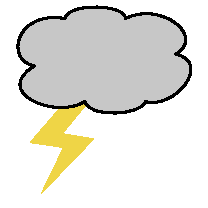
\includegraphics[height=\animationHeight]{animations/OliverLightning}
    	   \caption{Lightning.}
    	   \label{fig:animation:lightning}
    \end{subfigure}
    \begin{subfigure}{0.18\textwidth}
            \centering
            
\includegraphics[height=\animationHeight]{animations/OliverCar}
    	   \caption{Car.}
    	   \label{fig:animation:car}
    \end{subfigure}
    \begin{subfigure}{0.18\textwidth}
            \centering
            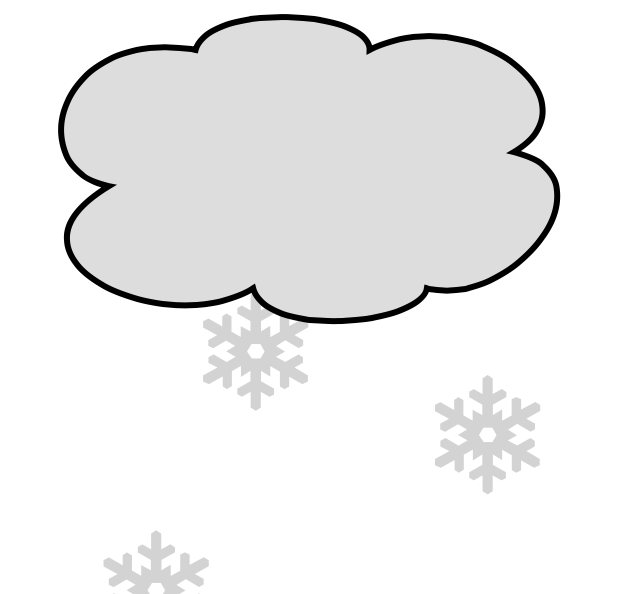
\includegraphics[height=\animationHeight]{animations/MacaronSnow}
    	   \caption{Snow.}
    	   \label{fig:animation:snow}
    \end{subfigure}
    
    \caption{Animations used as design tasks, in presentation order. Heartbeat expands in two beats; the cat's back expands as breathing and purring; lightning has two arhythmic bolts; the car oscillates up and down, and makes two turns: left then right; snow has three snowflakes float down.
    %See accompanying video for more detail.
    }
    \label{fig:animation}
\end{figure}



%%%%%%%%%%%%%%%%%%%%%
%
% SECTION: Results
%
%%%%%%%%%%%%%%%%%%%%%
\section{Results}
 
% 1. earlier you called them "designers" - might require qualification.
%
% 2. Later you mix in "I" with "P" subjects. I think (not sure) that you ran 13 subjects, but discarded 3 incompletes. This is a confusing way to say it; when you first identify the incompletes, along with P9, I can't tell what's what. Is it P1-P10 plus I1-I3? Indicate this right here where you identify subjects.
%
% 3. Better justify N=10. Later, it gets awkward when you note you only have 2 observations each. We know people will ask for more data; I don't think what's here is strong enough to counter. Need to indicate the COST of running a subject? relative to benefit? 20 would not be an unusual number for a psychophysics experiment. The point here is the analysis is hell. 

We targeted a study size of 10 complete participants for a balanced Latin square design, and a manageable sample size for rich, exploratory, qualitative analysis. % for an exploratory investigation.
13 untrained  participants were recruited: P1-10  (7 female, ages 22-35) completed all five tasks, while I1-3 (2 female, ages 29-45) 
% did not complete all designs due to time restrictions,  
only completed the first three % (heartbeat, cat, lightning) 
due to time restrictions.
% This may be due
Because I1-3 (and P9) all had the same interface order (\lo, \none, \vis, \hi, \select), we suspect that beginning with `sparse' versions gave insufficient insight into how to design quickly enough to finish the study. % into how to use examples.
I1-3 showed no distinct patterns beyond this; we leave their data for future analysis.  
%when we can follow-up with additional studies. 
% other than time constraints to not finish the study.
% After I1-3 failed to complete this order, P9 did complete it.
 
%


% We outline these, then describe the two main ways we saw examples used: 
% \kmC{SLC} % Note, this statement is repeated at start of (C) example use. I wonder if it would be better to give this preview in the Intro, but leave it out here?
% directly within each task as \emph{design starting points}, and indirectly over the session to \emph{learn how} to make VT designs.

\emph{Analysis and Data:} A team member % OS, should this be "team member?"
trained in qualitative methods analyzed screen recordings, interviews, and logs with grounded theory methods (memoing, open \& closed coding~\cite{Corbin2008}) and thematic analysis and clustering \cite{Moustakas1994}.
We visualized logs using D3 (\autoref{fig:archetype}). 
%
We chose a qualitative analysis because our goal was to capture the design process, not compare Macaron with previous tools.
% Qualitative analysis was chosen to capture the design process, rather than comparison with previous tools.
Our analysis exposed three major qualitative findings, discussed below.
%We now discuss our three major qualitative findings: 
% an archetypal process followed by participants, individual micro-interaction patterns, and strategies for example use.

%
%\kmC{slc} % I'm trying sticking this part about participants under "analysis", rather than as part of what looks like a usability comment. I believe you're not attributing the noncompletion to a lack of tool usability, but rather to task comprehension. But generally, the following statements are confusing and need to make a point more clearly.
%For each condition, participants were able to complete all 5 designs within their sessions, \kmC{[?? slc]  
%with one exception: three participants ran out of time, failing to finish all of P9's condition before P9 finally did.}
% P9 is one participant not 3. What does it mean that 3 (out of 10, this is not an exception it's a major proportion) failed to finish P9's condition before P9 did?  And how do the I1-3's count re latin square? 


\emph{Tool Usability:} Overall, the tool was well received, described as \qquote{P1}{easy to use}, \qquote{P5}{well made}, %\qquote{P7}{cool}, %\qquote{P7}{awesome},
\qquote{P9}{pretty neat}, \qquote{P3}{the templates help a lot}.
%\kmC{any more reserved comments to balance these, or more detailed insights about usability relevant?}


\emph{Completion time:}
%While we asked participants to click the ``start" button before they started designing, some clicked before browsing examples, and some afterwards.
%Therefore, w
%We calculated task time from handing off the mouse to the participant to the user's hitting the ``finish" button. %\kmE{located XX}.
Overall mean task completion time for P1-10 was 5m48s (median 4m48s, sd 3m52s, min 40s, max 18m23s).
%With two observations for each interface/task combination, 
We conducted two one-way ANOVAs on  completion time;
%,  with interface or task as factors.
%; diagnostics of normality (S-W test failed, but it's equal sample size and QQ plots showed limited violations. Also, Kruskal-wallis test corroborated ANOVA results) and homoscedascity (Levene's test) both passed.
%INTERFACE:(Shapiro-Wilk failed W=0.92, p=0.00192, but inspectino of QQ plots revealed limited skewness; Levene's test
%INTERFACE LEVENE TEST F(5, 44) = 0.8428 p=0.5268 
%INTERFACE ANOVA: $F(5, 44)=0.3596$ $p=0.8733$
%TASK S-W: W = 0.94902, p-value = 0.0311
%TASK LEVENe F(4, 45)=1.4966 p=0.2192
%TASK 
neither interface ($p=0.87$) nor task ($p=0.64$) had a significant effect. % on completion time.



\begin{figure}[tb]
    \centering  
    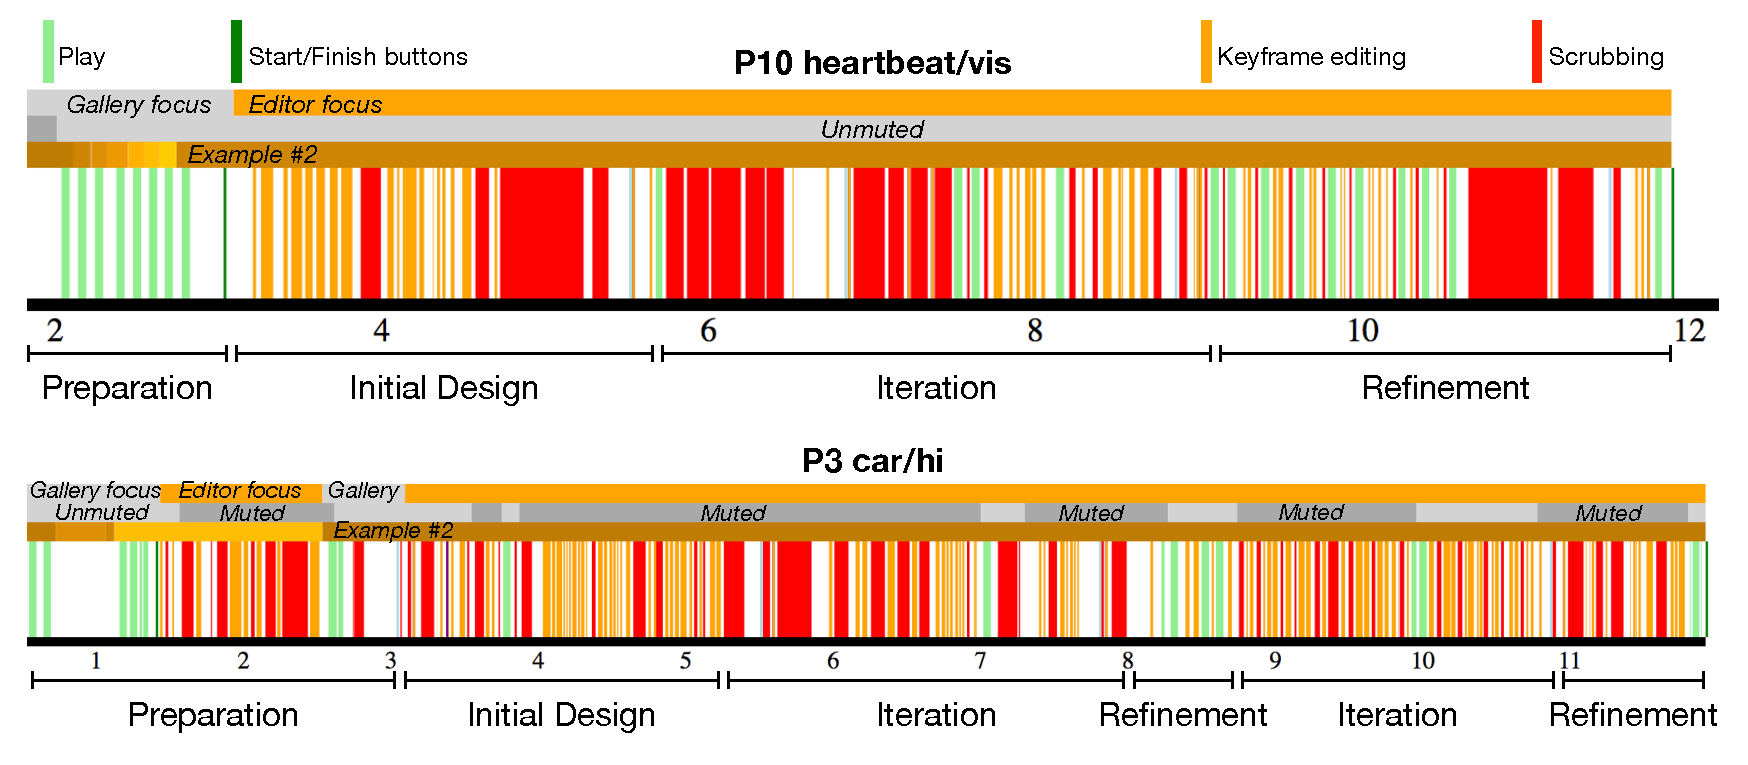
\includegraphics[width=\textwidth]{timelines/Example-Process-Diagram4}
    \caption{Log visualizations showing archetypal design process. Top: P10's heartbeat/\vis condition (an``ideal'' version). Bottom: P3's car/\hi condition (variations: a return to example browsing after editing, repeated refinement, muted editing).
    } 
    \label{fig:archetype}
\end{figure}


\begin{table*}[]
	\small
            \centering
            \begin{tabular}{p{0.5in}p{4in}}
%            \toprule
             \textbf{Prepare} & 
                All participants began with a problem preparation step \cite{Warr2005}. They played the animation to understand the problem, then typically looked at several (sometimes all) examples.
                %All participants browsed browsed at least one example once; 
                Only P2, P8, and P9 had a task where they did not begin with an example.
                Otherwise, participants browsed examples, chose a best match to the animation (\qquote{P7, heartbeat/\hi}{I was trying to find the best match with the visual}), then transferred into initial design. 
                Participants rarely returned to examples for more exploration; only P3 (car/\hi) and P5 (car/\lo) switched to a different example after beginning their initial design.
                Preparation is characterized by a large number of plays and example switches: on average, 47.45\% of all session plays were before the first edit (sd 30.15\%),
                %(todo- remove cases where I played),
                and participants switched examples an average of 6.75 times (sd 5.17).
             \\
    	    \midrule
    	    
             \textbf{Initial Design} & 
                Participants either used their example choice to help create their initial design, or ignored it because it wasn't close enough to what they wanted to do.
%                \kmC{SLC x2} 
                % 1. "what they wanted to do" suggests a vision that is apart from the example inspiration. Talk about that?
                % 2. In below: I'm so uncertain about what the gallery versions are (nondescriptive names) that it's hard to get import of the details reported. 
                Participants typically recreated the example in their editor by copy/paste of the entire design (P1,2,4-8,10) or sometimes a component (P3,10) in incorporable conditions (\hi and \select), or by manually recreating the design (P5,6) or a component (7,10) with \vis.
                In the \lo condition, we only observed P5 somewhat recreating an example.
                %LOW: P3 lightning/low?, P4 inspired
                Occasionally, participants would create a new design loosely based on the example rather than recreating it (P3,4,6-8), when using the \emph{Inspire} example use strategy (described later).
%                \textbf{TODO: Was this typically in Vis? (it was, need to count).}
             \\
    	    \midrule
    	    
    	    \textbf{Iterate} & 
                % After initial design, participants started iterating to develop their design.
                Participants refined designs with longer periods of editing typically book-ended by playing the entire design (discussed as ``real-time feedback"  micro interaction pattern).
            	In some cases, especially when the example was ``close enough", participants skipped iteration (\emph{Adjust} or \emph{Select} example use strategies, described later).
             \\
    	    \midrule
    	    
    	    \textbf{Refine} & 
                Smaller changes forecast design conclusion, e.g.,
            	incremental global changes: constant frequency (P1,2,5,6,10), alignment (P1,3,6), or pulse height adjustment (P1,3,8,10).
            	This step is sometimes visible in activity logs, as most participants (P1,3-10) exhibited more frequent plays of the entire design, and shorter periods of editing/scrubbing.
            	Occasionally, participants repeated larger iterations and refinement (P3 car/\hi, \autoref{fig:archetype}).
             \\
%    	    \bottomrule
            \end{tabular}
            \caption{Steps in observed archetypal design process.
            % \kmC{put Fig XX color codes here?? tiles under step names?}
            % \kmC{02.02: highlight word "example" in table, to show example appearance in process?}
            }
            \label{tab:archetypal:process}
        \end{table*}
        
        
%
% Archetypal Design Process
%
\subsection{Archetypal Design Process}
 % NEW 02.02  [see radical suggestion in next line!] devil's advocate: while I realize we've treated example use separately from design process (section A, B vs C) as I read A and B I start to wonder why they're here if our objective was just to look at examples use. Can you do a bit more to justify this, and perhaps allude to example influence on the design process? and/or, to the design process in (C)?  
 % [radical suggestion] In Table II, examples appear more than they do in the regular text. What if we highlighted every appearance of the word "example" in table II to illustrate this? You'd need an explanation in the caption, to effect we do this to help see where examples show up in the process we observed.
 %
Log visualizations (\autoref{fig:archetype}) show that users could and did employ Macaron for all key design stages: preparation, initial design, iteration, and refinement. %(\autoref{tab:archetypal:process}, 
% implying that it supported these steps.
All participants followed this sequence.
Some omitted one or more steps depending on personal style and strategies for using examples (below). % Verify - only a single step omitted by any one P, and all followed sequence? Earlier version sounded like "they all did the same thing except some did it differently" - seeking more concreteness about divergence.
We list observations of the basic process in \autoref{tab:archetypal:process}, to document behaviour and frame discussion.
% of example use and individual differences.
%\autoref{fig:archetype} shows an exemplar of this process.





%%%%% MOVED INTO TABLE %%%%%%%%
%     \subsubsection{\underline{Preparation}}
%     All participants began with a problem preparation step \cite{Warr2005}. They played the animation to understand the problem, then typically looked at several (sometimes all) examples.
%     %All participants browsed browsed at least one example once; 
%     Only P2, P8, and P9 had a task where they did not begin with an example.
%     Otherwise, participants browsed examples, chose a best match to the animation (\qquote{P7, heartbeat/\hi}{I was trying to find the best match with the visual}), then transferred it into initial design. 
%     Participants rarely returned to examples for more exploration; only P3 (car/\hi) and P5 (car/\lo) switched to a different example after beginning their initial design.
%     Preparation is characterized by a large number of plays and example switches: on average, 46.67\% of all session plays were before the first edit (sd 29.63\%),
%     %(todo- remove cases where I played),
%     7.78 example switches (sd 5.15).
% 	%⁃	TODO: how many unique examples (“examples viewed”??)
% 	%Participant rationale for choosing or browsing examples is discussed in more detail below. %  with direct example use in tasks.
    
%     \subsubsection{\underline{Initial Design}}
%     % After choosing an example,  usually the closest match to the problem domain or intended design, 
%     Participants either used their example choice to help create their initial design, or ignored it because it wasn't close enough to what they wanted to do.
%     \kmC{SLC x2} 
%     % 1. "what they wanted to do" suggests a vision that is apart from the example inspiration. Talk about that?
%     % 2. In below: I'm so uncertain about what the gallery versions are (nondescriptive names) that it's hard to get import of the details reported. 
%     Participants typically recreated the example in their editor by copy/paste of the entire design (P1,2,4-8,10) or sometimes a component (P3,10) in \hi and \select conditions, or by manually recreating the design (P5,6) or a component (7,10) with \vis.
%     In the \lo condition, we only observed P5 somewhat recreating an example.
%     %LOW: P3 lightning/low?, P4 inspired
%     Occasionally, participants would create a new design loosely based on the example rather than recreating it (P3,4,6-8), when using the \emph{Inspire} example use strategy (described later).
%     \textbf{TODO: Was this typically in Vis? (it was, need to count).}
%     %We describe this later under “Direct Example Use - Starting Point” as a spectrum of approaches: “ignore”, “inspire”, “template”, “adjust”, and “select”.

    
%     \subsubsection{\underline{Iteration}}
    
%     % After initial design, participants started iterating to develop their design.
%     Participants refined designs with longer periods of editing, either by itself or with scrubbing interspersed, typically book-ended by playing the entire design.
% 	They took time to \kmC{??: realize each new version of the design before giving them an overview.}
% 	% While the mute feature was rarely used, [KM: but, 3/7 did. That's not rare.} 
% 	P3, P4, and P7 all exhibited focused editing with mute enabled, unmuting for the bookended play sections; others did not use muting.
% 	In some cases, especially when the example was ``close enough", participants skipped iteration (\emph{Adjust} or \emph{Select} example use strategies, described later).

    
%     \subsubsection{\underline{Refinement}}
    
%     Smaller changes forecast design conclusion, e.g.,
% 	incremental global changes: constant frequency (P1,2,5,6,10), alignment (P1,3,6), or pulse height adjustment (P1,3,8,10).
% 	This step is sometimes visible in activity logs, as most participants (P1,3-10) exhibited more frequent plays of the entire design, and shorter periods of editing/scrubbing.
% 	Occasionally, participants would repeat larger iterations and refinement steps (P3 car/\hi), see \autoref{fig:archetype}.
% 	%Some participants skipped refinement(\emph{Select} example use strategy).
    %%%%%% END TABLE MOVED %%%%%%%

\subsection{Micro Interaction Patterns Enabled by Tool} 
Several small-scale  patterns further characterize behaviour within the archetypal process.

%\begin{figure}
%    \centering
%    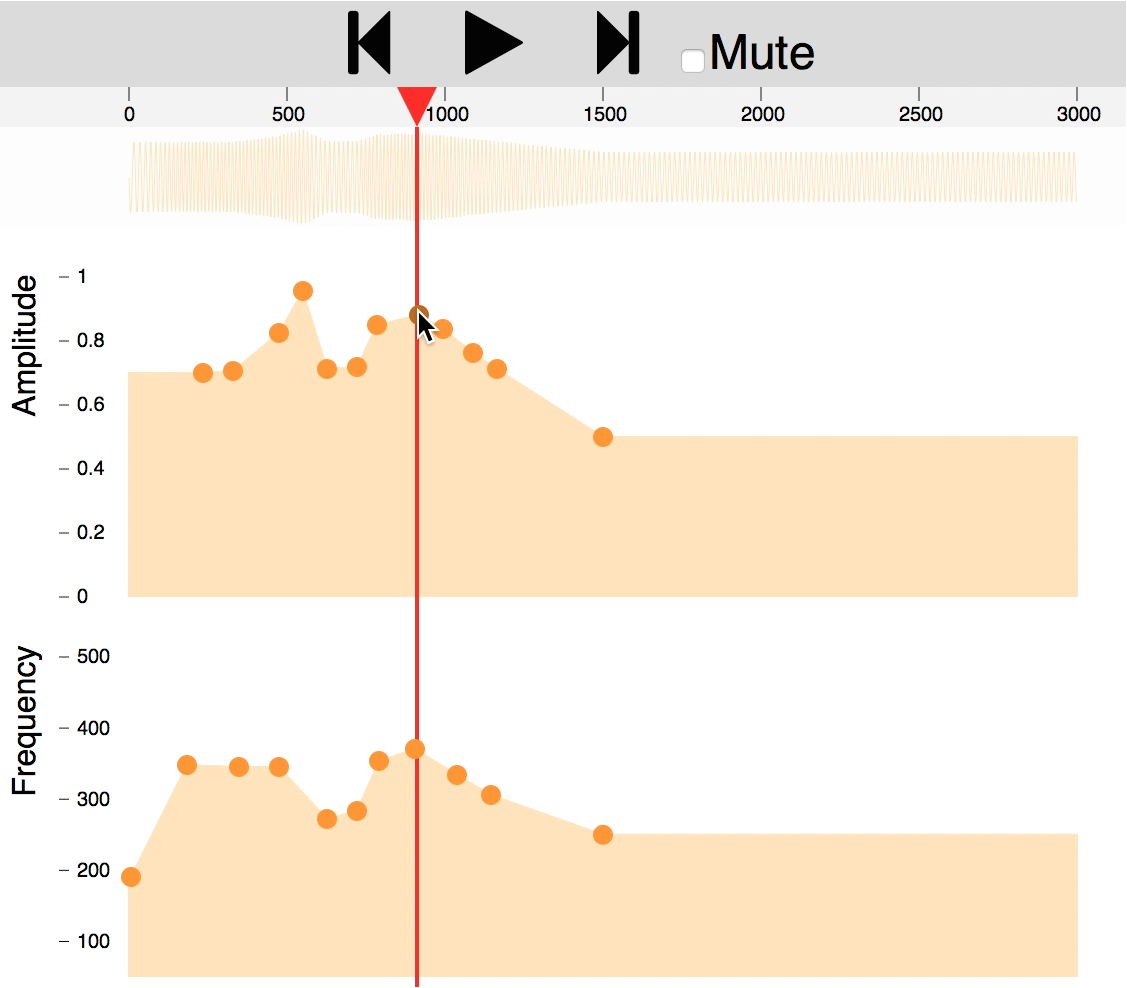
\includegraphics[width=0.24\textwidth]{Alignment-BetweenTracks-P13-Cat-None}
%    \caption{Participants used the red playhead for alignment, between animation and the multiple tracks (P9 cat/\none).
%    \kmC{Drop? slc} % The playhead shows up in other figures, can you reference it there? If so, may need to include the caption}
%    }
%    \label{fig:alignment}
%\end{figure}


\inlineHeading{Different paths through the interface}
% \subsection{Paths through the Interface}
%
% Participants navigated through the interface in different ways.
% We found three strategies that have later implications for design:
% by time, by component, and by track.
% With by time (\autoref{fig:path:bytime}, P1,2,3,4,7,9), participants march through the design, creating amplitude and frequency at the same time.
% With by component (\autoref{fig:path:bycomponent}, P1,4,6,8,10), participants develop and iterate on part of a design, then repeat or copy and paste the component later in time.
% With by track (\autoref{fig:path:bytrack}, P2,3,6,7,8,9,10), participants work through an entire track (typically amplitude) before working through the other one.
% These different strategies are often combined; for example, P6 developed their car/\lo component by track (amplitude, then frequency).
%
%% Further enforcing flexibility, participants frequently used copy and paste to replicate points in time (containing points from one or both tracks), but P1,3,7 also brought up being able to copy and paste between tracks:
%% \qquote{P7}{The one thing I found missing was copy and pasting between amplitude and frequency}.
%    % Participants navigated through the interface in different ways. 
%
%
    We saw three design-path strategies. % that have later implications for design:  %  time,  by component,  and by track.\\
    \par -- \emph{Time} (\autoref{fig:path:bytime};  P1,2,3,4,7,9): proceed through the timeline,  creating  amplitude  and  frequency  at  the  same  time.
    \par -- \emph{Component} (\autoref{fig:path:bycomponent}, P1,4,6,8,10): iterate  on  a  design element,  then  repeat  or  copy/paste it later in time.
    \par -- \emph{Track} (\autoref{fig:path:bytrack},  P2,3,6,7,8-10): proceed through one entire \emph{track} (typically amplitude), then the other one. 
    
 \noindent Strategies were often combined hierarchically. P6 developed a car/\lo component by track (amplitude, then frequency).
    Wanting additional flexibility,   %participants  used copy/paste to replicate points in time (re-using points from one or both tracks),  but 
    P1,3,7  requested  copy/paste  \emph{between}  tracks: \qquote{P7}{The  one  thing  I found missing was copy and pasting between amplitude and frequency}.
 


\begin{figure}[Htb]
\centering
\begin{subfigure}{4.5in}
    \centering
    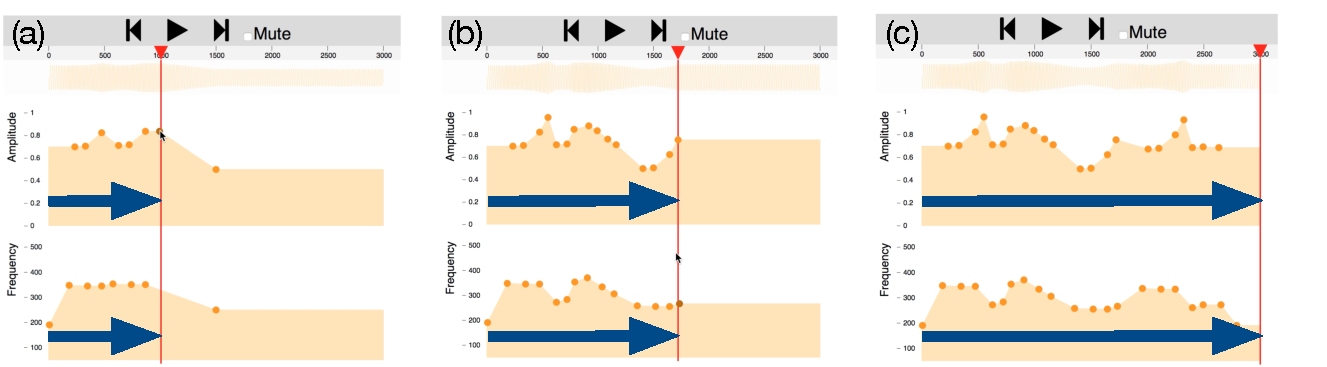
\includegraphics[height=1in]{paths/Path-ByTime}
    \caption{P9's cat/\none design progressed sequentially in time.
    Note the red playhead helping alignment in (b).
     }
    \label{fig:path:bytime}
\end{subfigure}

\begin{subfigure}{3.5in}
    \centering
    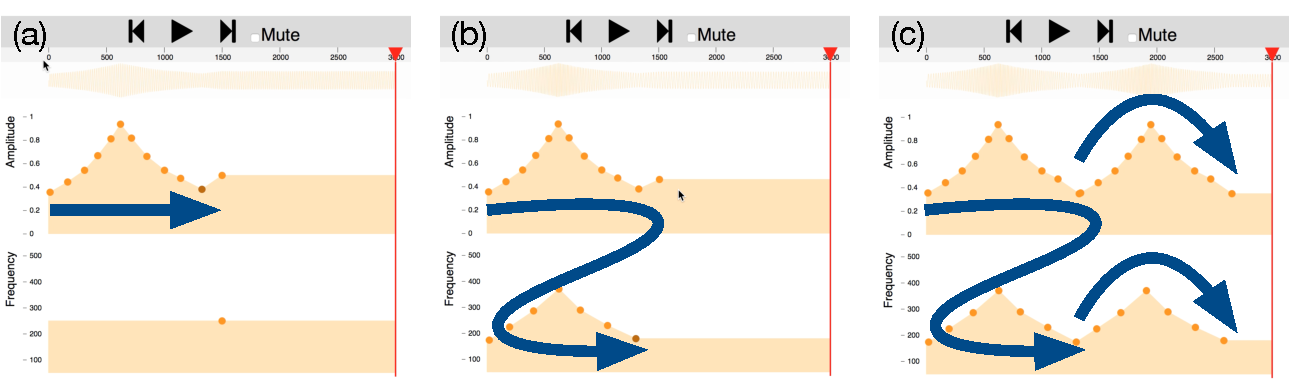
\includegraphics[height=1in]{paths/Path-ByComponent2}
    \caption{P6's car/\lo design progressed by component, developing the component then repeating it.}
    \label{fig:path:bycomponent}
\end{subfigure}

\begin{subfigure}{4.5in}
    \centering
    \includegraphics[height=1in]{paths/Path-ByTrack}
    \caption{P10's heartbeat/\vis design progressed by track. Amplitude was developed first, then frequency.
    }
    \label{fig:path:bytrack}
\end{subfigure}
\caption{Participants created their designs using different progression paths, suggesting flexibility.}
\label{fig:path}
\end{figure}
%
   \begin{figure}[Htb]
    \centering
    \includegraphics[height=1.75in,width=4in]{realtime/RealTimeFeedback}
    \caption{Participants used real-time feedback to explore, both (a) in time by scrubbing back and forth (P3 lightning/\lo), and (b) by moving keyframes (P10 heartbeat/\vis).
%        \kmC{lose some whitespace? slc.} % do you need the (a), (b) etc in Figs 6, 7, 9? Would get you 3-6 lines of vertical compression.
        }
    \label{fig:realtimefeedback}
\end{figure}
    

%    \kmC{slc} % KM 11.07 1311 Does this par belong under Micro Interactions? clarify why it's a path-thru-interface if not.
    Further showing diverse workflows, participants requested more powerful controls to work with keyframes as a group, such as widen (P5), reverse (P7), shift everything (P9), move up/down and smooth (P4). % these requests  by saying the more power we have, the better: \qquote{P1}{It's always good to have more control over what I can adjust}.
    %This could have an affect on how participants choose their examples or their approach for initial design:
%    \qquote{P7}{None of [the examples] came close...the one I selected was the exact inverse of what I wanted}.
%    \qquote{P7}{The [example] I selected was the exact inverse of what I wanted}.
    Other requested features include looping (P1), hovering over a point to see the value (P1), more detail through a zoomable interface (P4). 
    %OS CUT? P4 discovered and heavily used left/right arrow keys to navigate the timeline, a feature that had not been disclosed but remained in the tool from development.

\inlineHeading{Alignment and Copy/Paste are Precise, Convenient}
%    Participants described both alignment and copy/paste as important features.
    Precision was valued; alignment and copy/paste were used to achieve it.
%       
%       \kmC{is this a novice thing?? SLC} % I wonder if precision desire comes from the tool affordance, and transfer from other editing (visual) where precision can really count. It might be that a precise design is indistinguishable haptically from a nonaligned one, but these subjects don't know that yet.
%       
    Alignment was sought both in time and to keyframe values.
    A common technique (\autoref{fig:path:bytime}b) was to use the red playhead like a plumb-line to align keyframes with animation features (P1-5,7,9,10) and between the two tracks (amplitude and frequency) (P3-5,7,9,10): \qquote{P2}{Using that red arrow thing and placing the dots when it makes the heartbeat}.
    Some participants, including those who used the plumb-line, requested
    %P1,2,6,7,8,9
    %Six participants requested even 
    more refined alignment features: \qquote{P1}{I couldn't keep it straight}. %\textbf{CONFIRM!} \kmC{slc} % Were requestors the same ones who made use of plumbline, or were they ones who hadn't discovered it? i.e. was plubmline enough?
    % Several participants requested alignment features: shift to move in only one of x or y; anchors; alignment of video.

    Copy/paste was used for improved  work efficiency (especially helpful during initial layout or when creating long or repeating designs)
    %\qquote{P1}{If you want to create something that's longer you might want copy and paste},
    %\qquote{P2}{It was easier to use the examples, and it felt like matched, not exactly, but enough}.
%    \qquote{P6}{That was easy, I just copy and pasted the entire thing}.
    and precision:
    \qquote{P6}{Copy and paste...was also the most precise, because if you feel like it's a perfect fit, you can use it exactly}.
    Correspondingly, conditions without copy/paste (\emph{i.e.}, \lo and \vis) took additional effort:
    % \qquote{P5}{It's harder than the previous ones because there's no copy and paste}.
    \qquote{P5}{It's harder...because there's no copy and paste}.
%    \qquote{P6}{That was a little tedious}.
    %Indeed, even 
%    Power features (e.g., keyframe typing) were used mainly for alignment: \qquote{P1}{maybe, if I want to align stuff}.
    Precision also depended on context: %\qquote{P9}{If it was used for monitoring someone's health, you would have to be very accurate}.
    \qquote{P9}{For monitoring someone's health, you would have to be very accurate}
    %, \qquote{P4}{I find [copy and paste] to be a useful but not priority functionality for me...I feel like vibration is less precise compared to vision}. % because I don't know if it's right or wrong, but I feel like vibration is less precise compared to vision}.

    

	%⁃	Copy and paste was often cited making things easier and less tedious, especially for larger tasks. Speed: less mentioned, but related, was that copy and paste sped up the process. Precision: Because c+p exactly replicated the source material, it was described as more precise.. This is interesting because P4 said copy and paste was less important to her, but that’s because she considered vibration to be less accurate than other modalities (connected to the gist/focus or prefeel/render). Precision is also connected to other features: alignment (which subsumes entering values), purpose of the design (medical vs. toy P9)
	%⁃	Several participants requested alignment features: shift to move in only one of x or y; anchors; alignment of video. Participants also described one major approach aligning their vibrations to events in the animation. This is consistent with our observations; we saw several participants use the read playhead to both line up keyframes with video events, and to align keyframes between amplitude and frequency.


\inlineHeading{Editing and playback}
During iteration, participants edited in bursts of primarily scrubbing activity, bookended by full playthroughs.
They took time to realize each new version of the design before observing an overview.
            	% While the mute feature was rarely used, [KM: but, 3/7 did. That's not rare.} 
    % KM 11.07 1314: confused about this section. 
    % 1. above sounds like all participants did both levels at different times.
    % 2. below, what you drill in on is scrubbing. Now, I think what you might be saying is that while everyone did focus work (they must have done), only some chose to scrub as they focused. If that's so (not sure) then is this section about scrubbing during focus work (as a strategy that M supports, but only some people liked) or about focus vs overview switching seen in everyone?
   		When editing, participants scrubbed back-and-forth, varying speed (P1-4,7,9,10), and dragging keyframes to try ideas out (P1,3,4,7,9,10) \autoref{fig:realtimefeedback}.
    This feature was valued by those who used it: \qquote{P1}{The real-time part is pretty important};
%\qquote{P1}{When I adjust it I can feel how it changes, the real-time part is pretty important};
    some rarely played, showing more frequent or longer periods of scrubbing instead (P2,9,10).
    %P2 had difficulty working with frequency until the researcher suggested trying it: \qquote{P2}{Ah, okay, the vibration disappears at a higher frequency}.
    Others rarely scrubbed (P5, P8), possibly to have an overall sense of the design: \qquote{P8}{Trying to get a general sense of how it might feel}.
%    P5 only scrubbed back-and-forth when reminded of the tool's capability in their cat condition; %, but did not continue to do this afterwards, and did not try out keyframe values in a focused way.
%    P8 intentionally did not use scrubbing outside of the training task, instead playing frequently: \qquote{P8}{Trying to get a general sense of how it might feel}.
    %P4 remarked on target of focus: \qquote{P4}{I was mostly creating it by looking at the animation, so during creating I didn't really try it out a lot}.
            	P3, P4, and P7 all exhibited focused editing with mute enabled, unmuting for the bookended play sections; others did not use muting.



%\subsubsection{\underline{Feedback: Scrub or Press Play}}
%    % KM 11.07 1314: confused about this section. 
%    % 1. above sounds like all participants did both levels at different times.
%    % 2. below, what you drill in on is scrubbing. Now, I think what you might be saying is that while everyone did focus work (they must have done), only some chose to scrub as they focused. If that's so (not sure) then is this section about scrubbing during focus work (as a strategy that M supports, but only some people liked) or about focus vs overview switching seen in everyone?
%    When working in a focused way, participants scrubbed back-and-forth, varying speed (P\osC{1?2?,}3,4,7,9,10), and dragging keyframes to try ideas out (P1\osC{?2?},3,4,7,9,10) \autoref{fig:realtimefeedback}.
%    This feature was valued by those who used it: \qquote{P1}{When I adjust it I can feel how it changes, the real-time part is pretty important}.
%    %P2 had difficulty working with frequency until the researcher suggested trying it: \qquote{P2}{Ah, okay, the vibration disappears at a higher frequency}.
%    Participants who preferred to scrub rather than play the entire design showed more frequent or longer periods of scrubbing (P2,9,10) instead of playing.
%    
%
%    
%    This behaviour seems to be related to personal preference.
%    P5 only scrubbed back-and-forth when reminded of the tool's capability in their cat condition; %, but did not continue to do this afterwards, and did not try out keyframe values in a focused way.
%    P8 intentionally did not use scrubbing outside of the training task, instead playing frequently: \qquote{P8}{Trying to get a general sense of how it might feel}.
%    %P4 remarked on target of focus: \qquote{P4}{I was mostly creating it by looking at the animation, so during creating I didn't really try it out a lot}.

\inlineHeading{Encoding and Framing}
%\kmC{SLC - Examples?} % [02.02] Can we bring this back to examples more?
% [pre-submission] the encoding thing seems potentially very important, and not really focused on here. Maybe highlight in future work. Can examples, or simply encoding matches between haptics and other modalities, help us understand natural mappings or translations between modalities? 
    % Participants had different strategies when tackling their designs.
    Some participants encoded parameters using consistent rules, often aligned to events like heartbeats or lightning bolts.
    Others sought to create moods or metaphors for sensation.
    
   Encoding %\kmC{SLC} % What (which of previous two strategies) was visible? It sounds like all examples of consistent rules (but crashes on lightning strikes could also be metaphor, but that would make it a combined strategy). Do you have other examples of mood/metaphor? 
   was most visible in the lightning task, where participants represented lightning bolts in regular ways: %with pulses of consistent height:
   %, sometimes representing left and right lightning strikes differently (different heights or shapes):
   \qquote{P9}{if there was a lightning bolt on the left, I put amplitude and frequency a little longer than a lightning bolt on the right}.
   When the animation had two simultaneous bolts, several (P2-4,7,9) encoded it by superimposing two bolt representations on top of one another.
   Participants were forced to reframe their encoding strategy:
   \qquote{P7}{...two [lightning bolts]...I divided it into two equal partitions, .6 and 1}.
%   \qquote{P7}{...two [lightning bolts] at one particular snapshot, that is why I divided it into two equal partitions, .6 and 1},
%   \qquote{P9}{if there were two bolts I tried to make double amplitude and frequency but I ran out of space}.
   
%   Encoded designs varied, either encoded in shape or in parameters.
%   We often observed frequency mirroring amplitude (as observed in \autoref{} and \autoref{}.
%   Sometimes, the two were developed in concert, somewhat mirrored and sometimes varied (as in \autoref{}).
%   Finally, sometimes parameters encoded different features.
%   P1 used amplitude to represent the bumpiness of the car, and frequency to represent the turns.
   
   Encoding failed when participants did not find a direct mapping:
   %\qquote{P9}{Normally you don't think of snowflakes in terms of vibrations},
      %P7 couldn't resolve representing three snowflakes with two parameter tracks: 
      \qquote{P7}{When the three [snow flakes] come together I think my strategy broke down}. %, because there are only two choices, amplitude and frequency}.
%   \qquote{P2}{it felt like the snowflakes were going in a wave}.
   Metaphors helped in these cases.
   Car took extra imagination, either for the experience of driving (P6, P8, and P9 didn't drive), %, but designed for what they imagined),
   %it to be like;
   or because it's hard to %P1 knew what it felt like to drive, but didn't
   \qquote{P1}{know what it would feel like on the wrist}. %\kmC{SLC} % so what did they do? was this then a failure? Did they divert to a metaphor/mood approach? If so, would a general approach be: first try to encode, if that fails try a metaphor/mood? 
   %
%   There was a strong tendency to ``focus on the visual" task:  P2, P4, P7, P8. 
   %
%   We do not yet know if this was due to abstractness of the sensation, the slower speed, or amount of features present in the animation.
%   More general metaphors were used instead of a direct encoding.
   P6 describes her process for both lightning and snow as using mood: \qquote{P6}{...what I think the mood is...like snow fall, it's kinda like, very gentle and calm}.
   

   

   
	%⁃	Some participants, however, did not focus on alignment in their designs, instead focusing on general impressions to create a “mood”. [connect to focus/gist above?] [connect to framing and metaphor below?]
	%⁃	ENCODING???
	%⁃	Participants demonstrated framing, structuring the problem to find an appropriate tack to continue. In accordance with Schön’s theory of “seeing the problem in familiar terms”, participants often drew parallels with earlier tasks: 

	



%
% Example Use
%
\subsection{Example Use}  % Can you allude to design process in this section, so it feels more like (C) is building on (A) and (B)?  Then tell reader this will happen in framing?
% The alternative versions of Macaron did not influence process along our theoretical dimensions (visibility and incorporability) as clearly as we hoped. % as we had hoped. %demonstrate a clearly observed comparison.

As seen, examples played a major role in users' design processes.
%that users' natural tendencies, supported or stunted by these constraints and opportunities, would appear as differing strategies and use patterns.
Analysis revealed the effect of examples to be more nuanced than %d picture appeared in analysis.
%Presence / absence of these factors in the tool variants worked well to elicit strategy experimentation and consequent reflection 
%% (e.g., missing an element when it was gone).
a one-to-one mapping of the theoretical dimensions of incorporability and visibility.
%Other dimensions, %(e.g., a concept of design \emph{editability} as distinct from example incorporability, as well as task- and user- centered variables). 
Emergent themes were instead organized on the \emph{role} of examples: %, rather than interface features:
%, by which we frame our  discussion:
as a \emph{direct starting point} for each design; and
to \emph{indirectly scaffold learning} throughout a session.
The latter was related to additional themes: task difficulty and individual differences.


% didn't line up perfectly with task process that people used; and other factors, were hinted at like task difficulty and abstraction, user confidence in their abilities (designerlyness), 

%difficulty (from task, interface, and personal confidence/learning)
%task (task difficulty (complexity and abstraction), user strategy (encoding, metaphor), confidence, learning)
%

\inlineHeading{Direct example use -- task starting point}
   When participants \emph{prepared} for each task by browsing to find a best-match example, then using it as a starting point, they did this with a spectrum of strategies. These strategies, elaborated in \autoref{tab:direct:example:strategies}, range from Ignore (examples not used) to Select (an example was the final design). 
 %   \osC{quantify:slc}
    %OS 10.20 NEED TO QUANTIFY EACH OF THESE, INCL. correlation to interface.

        \begin{table}[]
        \small
            \centering
            \begin{tabular}{p{0.5in}p{4in}}
%            \toprule
             \textbf{Ignore} & 
%                      \kmC{SLC}  % Is "ignore" the best term for this? I'm thinking of case where they browsed and looked, but didn't find what they want. This seems not so much ignoring, as trying but dissatisfied with examples. Should these be two different cases - deliberate ignoring, vs unfound? Or, "unused" as strategy name?
                Deliberately do not choose an example,
    	         through either lack of match:
    	        \qquote{P1}{I didn't [find] the examples that I wanted};
    	        a desire to challenge themselves or be creative:
%                \qquote{P8}{...difficult to replicate, so I just wanted to do my own thing};
		\qquote{P9}{I wanted to do my own thing!};
               or difficulty in using the examples. 
%               \kmC{mapping weak. positive: creativity. negative: inadequate example library? }
    	        \\
    	    \midrule
    	    
             \textbf{Inspire} & 
                Choose an example, but do not explicitly copy/paste or replicate it in the editor; instead, design based loosely on example parts, sometimes as an adaptation from memory: \qquote{P6 car/\lo}{I just tried to remember what the keyframes were like before, and then I modified it}.
%                \par \kmE{Requires: high-viz, low-incorp, high-edit.} 
                % Attributes of our old dimensions show up. When OS says it wasn't a ``thing'' in the analysis, does this mean there wasn't alignment of "inspire'' strategy with hi-vis, low incorp usages?
             \\
    	    \midrule
    	    
    	    \textbf{Template} & 
                Choose an initial example, but alter it considerably.
            	In this case, participants use the example to expedite the process. %, but still modified it substantially.
            	%, such as P7 inverting his waveform.
%            	\par \kmE{Requires: high-viz, high-incorp. high-edit}.
             \\
    	    \midrule
    	    
    	    \textbf{Adjust} & 
%    	                \kmC{slc} % ?? due to disinterest, or really liked example? Were these other methods not wanted at other times?}
                Find an initial example, skipped major iteration and went directly to the refine stage, sometimes because the example was a close match.
                To enable this, some participants wanted a more powerful manipulation methods, like inverting (P7). % than was available.
                %, like stretching, or inverting (P7).
%                \par \kmE{Requires: high-incorp, high-edit; viz unclear}
             \\
    	    \midrule
    	    
    	    \textbf{Select} & 
                Copy/paste an example (or manually recreate it), % and manual recreation otherwise,
                then do not modify;
                sometimes because the example seemed to match:
	                \qquote{P5}{...copy and paste, then confirmed it was the same.}
%	                \qquote{P5}{I played this first, then matched the graph, then copy and paste, then confirmed it was the same.}%, and I think it is the same.}
                	%\qquote{P2}{The vibrations follow one of those patterns}.
                	%This could occur after a significant deliberation period (P7 played example X Y times, adjusted, then undid his actions).
                	%Participants sometimes explained this as they did not feel they could do better (P?). %\kmC{Other cases? disinterest??}
%                	\par \kmE{Requires: high-incorp, indifferent viz, editability.}
             \\
%    	    \bottomrule
            \end{tabular}
            \caption{Strategies used by participants to directly use examples as a starting point.
            Ignore and Inspire did not start with copy/paste; Template, Adjust, and Select did, with varying amounts of editing afterwards.
            When copy/paste was not available, manual re-creation was used as a stand-in.
            %, with mappings to original and augmented theoretical example-access dimensions of visibility, incorporability and editability.
            }
            \label{tab:direct:example:strategies}
        \end{table}
    	
    	
    %%%BELOW MOVED INTO THE TABLE%%%%%
%     	\emph{Ignore: } \kmC{SLC}  % Is "ignore" the best term for this? I'm thinking of case where they browsed and looked, but didn't find what they want. This seems not so much ignoring, as trying but dissatisfied with examples. Should these be two different cases - deliberate ignoring, vs unfound? Or, "unused" as strategy name?
%     	Deliberately do not choose an example.
%     	Sometimes it was because there was no match:
%     	    \qquote{P1}{I didn't [find] the examples what I wanted},
%     	    \qquote{P9}{I didn't use [an example] because I didn't feel any of them were applicable to the snow flake}.
%     	Or through a desire to challenge themselves or be creative:
%          \qquote{P8}{...difficult to replicate, so I just wanted to do my own thing},
%          \qquote{P9}{I wanted to do my own thing!}.
%         Another reason was difficulty when trying to work with examples:
%          \qquote{P2}{I didn't know how, or I just kinda forgot}.
         
         
%     	\emph{Inspire:} 
%     	Choose an example, but do not explicitly copy/paste or replicate it in the editor; instead, design based loosely on example parts, sometimes as an adaptation from memory: \qquote{P6 car/\lo}{I just tried to remember what the keyframes were like before, and then I modified it}.
%     	%Or done when viewing keyframes (\textbf{TODO}).
    	
%     	\emph{Start/template:} 
%     	Choose an initial example, but alter it considerably.
%     	In this case, participants use the example to expedite the process, but still modified it substantially, such as P7 inverting his waveform.
% 	%(what was their motivation? this is the most vague, how does it differ from adjust??)
    	
%     	\emph{Adjust:} 
%     	Find an initial example, skipped major iteration and went directly to the refine stage.
% 	%Occasionally this was challenging, 
% 	%\kmC{?? due to disinterest, or really liked example? Were these other methods not wanted at other times?}
% 	At this point, participants sometimes wanted a more powerful manipulation method than was available, like stretching (quote) or inverting (P7), or filters (quote).
    	
%     	\emph{Select:}	
%     	Choose an example and do not modify. Sometimes this was because the example seemed to match:
% 	\qquote{P5}{I played this first, then matched the graph, then copy and paste, then confirmed it it was the same.}%, and I think it is the same.}
% 	%\qquote{P2}{The vibrations follow one of those patterns}.
% 	This could occur after a significant deliberation period (P7 played example X Y times, adjusted, then undid his actions).
% 	Participants sometimes explained this as they did not feel they could do better (P?). %\kmC{Other cases? disinterest??}
	
%   % 	Copy/paste vs. Visualization
% %    	These 5 techniques varied based on interface and stage in design. participants did TODO CORRELATION    
     %%%%%% END TABLE MOVED %%%%%%%
    
    
    

   
   
   
    \inlineHeading{Indirect example use -- observe how to design}
    Over the course of the session, participants used % examples or 
    underlying structures of examples to understand how to design VT icons. % to relate this structure to their feel. 
    This was most evident in the \none or \lo condition after participants were first  exposed to examples: 
    %\qquote{P4 car/\none}{I don't know if it's cheating, but I sort of remembered, there is one vibration in this session that's very similar to this, so I sort of picked it up?},
    \qquote{P4 car/\none}{I sort of remembered}.
%    \qquote{P5 cat/\none}{I kind of mocked the examples that I saw before},
    %\qquote{P6 car/\lo}{I just tried to remember what the keyframes were before}.
    Some % participants 
    explicitly described learning: % within a session: 
    \qquote{P9 lightning/\vis}{It gave me a general idea of thinking in big shapes rather than little dots}.
   % Others specifically commented on learning how to use frequency:
    %\todo{}

    
    Most participants commented on the difficulty or ease of their task (P1-5, 7-9). Task difficulty was connected learning (\qquote{P4 snow/\lo}{It's easy...maybe it's more experience}) and individual differences.
    Some people were motivated to learn, and challenge themselves; others were not.    
    
    Connections between these factors are complex and difficult to unravel with this data.
    We speculate on the utility of flow theory
    % However, this suggests the theory of flow 
    \cite{Csikszentmihalyi1996} as a useful lens to connect these issues, as it considers creativity, education, and the relationship between perceived challenge and perceived ability.
    We plan to use it to frame future exploration.
    
%    Another confounding factor with learning is differences between the tasks themselves, and what characterizes their difficulty: complexity, abstractness s
    
    
    
    
    
%        Examples were important to this, building a repertoire and helping to explain the symbolic domain of the tools, especially frequency (quotes).
%Part of this was building their repertoire,... some of this was due to frequency; 
%    	⁃	Task difficulty?
%    	⁃	Individual differences?
%    	⁃	challenges?
%    	⁃	Participants readily gave feedback on the difficulty of each task. Difficulty depended on the interface (P5/cat, “harder than before, because there were no examples”), the task (P9/cat, “harder, because the cat’s motion, it’s less noticeable”), and the participant’s experience (P4/snow “the interface is not specifically better than any previous ones â€Å%  but I say it’s easier because I’m just getting better with it”).
%    	⁃	
%    	⁃	flow?
    		% \subsection{Motivation}
            % Some participants seemed knowledgeable, or generally ``well-behaved" designers, comfortable with the interface and typically following the archetypal process.
            % Other participants had different motivation, which we noticed in two groups: the ``mathophobic" group, and the ``individual
            
            %     \subsection{Mathophobic}
            %     P2, any others?
                
            %     \subsection{Individualistic}
            %     Need to talk about using examples or not.
            
            % \subsection{Repertoire}
            % discuss Schon, connect to visualization
            
            % \subsection{Task difficulty (and framing?)}
            





% %%%%%%%%%%%%%%%%%%%%%
% %
% % SECTION: Discussion
% %
% %%%%%%%%%%%%%%%%%%%%%
% \section{Discussion}

% What to put here?


%%%%%%%%%%%%%%%%%%%%%
%
% SECTION: Implications for Design
%
%%%%%%%%%%%%%%%%%%%%%
\section{Discussion}
We discuss implications for design, then limitations we hope to progress on with future work. %including observed themes and online deployment.

\subsection{Implications for Design}
    
    %Expose examples
    \subsubsection{Expose example structures for learning}
    When exposed to examples' underlying structure, participants are able to build their repertoire and learn VT design conventions like \qquote{P9}{big shapes}.
    %\kmC??: conventions (quote about using big shapes)}.
    Such scaffolding is particularly crucial in an environment where experienced VT designers and training possibilities are rare. % , typically available only at select universities.
    Whether through exploratory tool use or structured with online training programs, examples can expand the VT design practices available to novice designers.
    
    %templates
    \inlineHeading{Examples as templates}
    Participants typically copied an example first before iterating and customizing,
    %\kmC{?? SLC: This was contrary to our initial hypothesis,} % Was this a hypothesis? I can't find it or any others.
    suggesting a template model of modifiable source documents as a way to expose structure and reduce effort for designers.
    %A more accessible model for using examples might be able to select and open them, like boilerplate or templates. %\kmC{SLC} % At least one of your galleries did this, right? Is this an implication for design tools, or for use of examples? Restate less ambiguously.
%    This model is appropriate for larger modifications, and for the smaller changes of the Adjust strategy using global tools or filters \cite{Seifi2014}.

    
    %templates
    \inlineHeading{Example Recommender}
    The time participants spent searching for the suitable examples suggests a recommender system could be very valuable. %\kmC{SLC} % again, is this a design tool implication?
    AI techniques might recommend examples similar (or dissimilar) to a source stimuli, as with previous tools in other sensory modalities \cite{Lee2010a} and VT 
    %The challenge of supporting browsing for haptic stimuli has been broached through
    visualization tools like VibViz \cite{Seifi2015}.
    
    %examples in context
    \inlineHeading{Clarify example context}
    % 3However, more powerful recommendation tools should not compromise context.
    Participants often repeated gallery searches for each new animation; they needed to compare examples alongside the target graphic.
    In addition, though our examples were designed independently of our animation tasks, some participants showed confusion about whether they were supposed to match. %\kmC{?? SLC}. % Don't understand previous. They thought there was a whole new gallery of examples each time they got a new animation? Because they had incompletely explored previously, or couldn't recall seeing them before? 
    %\textbf{TODO: Put in example section}.
    Clarifying the context for each example, by presenting it either in connection to its original design goal or as a candidate for the participant's current goal, will help participants choose an example.
    %New recommender or navigation tools could benefit from including this context.
    
    
    %hideable
    \inlineHeading{Hideable examples}
    Some participants wanted to be individualistic with their designs and actively disliked the most powerful \hi condition, saying that the \none condition was cleaner, or that while examples were helpful to learn, they felt ``more creative" with fewer examples present.
%    A simple solution to this design problem could be
    A hideable gallery, which can be opened when needed but kept hidden otherwise, could accommodate user preference.
    %This capability could also be personalized, where participants could intentionally restrict visibility or incorporability.
    An intelligent gallery could even time example appearances or suggestions to occur at helpful design stages, e.g., by recognizing by activity patterns \cite{Warr2005,Dow2011}. %: example timing study, brainstorming separately then coming together papers).
    
    
%
% Implications for VT Design
%
% \subsection{Implications for VT Design Tools}
    
    % Prefeel
    \inlineHeading{Realtime ``prefeel" then render} % Prefeel and Render}
    Macaron's real-time feedback supported exploration, with full play-throughs providing an overview or  evaluation in-between editing sessions.
    %Participants typically worked in focused, sustained bursts that included real-time experimentation: scrubbing and keyframe modification. %\kmC{SLC} %% What is 'movement of keyframes'?
    %This exploratory editing was typically bookended by full play-throughs of animation and vibration.
    %This suggests that real-time exploration was important in focused work, and full play-throughs important for an overall view.
    %\kmC{SLCx2} 
    % 1. Not following. Do the full play-throughs indicate that the real-time scrubbing was not necessary? How does that follow? 
    % 
    % ** 2. Below it sounds like in contrast, you're saying that the pre-feel is pretty important. I'm confused about the overall point of this section.** 
    In addition, P4, who was familiar with haptics, felt that the scrubbing synthesis  was ``muddy" relative to waveforms pre-rendered with audio tools -- a common challenge, noted also by the researchers but deemed suitable for this study.
    %
    % Because real-time synthesis sometimes falls short compared to rendered sensations,     this process suggests a feedback model based on 
    While we hope this technology deficit inspires improved realtime rendering algorithms, it also suggests an explicit workflow compromise.
    Many video editing and compositing tools show a low-resolution previsualization in design mode; a clip is then fully rendered for playback.
    For tactile design, coarse, ``prefeel" sensations would be synthesized for immediate feedback during a rough design stage, and a high-fidelity rendering generated for less frequent play-throughs.
    This %may have marginal gains for a short, vibration-based editing, but could pay off when using 
    could help computationally demanding, perceptually-based models or multi-actuator setups (e.g., tactile animation \cite{Schneider2015} as a prefeel for tactile brush \cite{Israr2011a}).

    % Wide Walls
    \inlineHeading{Tool flexibility}
    Macaron was used in very different ways depending on the participant.
    % % Multiple Avenues
    % \subsubsection{Multiple Avenues}
    %In particular, participants had two strategies for developing their design: by track, by working with amplitude exclusively, then with frequency exclusively; and by time, by working with amplitude and frequency in tandem, marching along time or copying and pasting to repeat a designed example.
    Some progressed by time, by track, by component, or a combination thereof.
    Some mirrored  frequency and amplitude, using them together, while others used them to express different ideas. % (P1 used frequency to express rumbling in the car animation, and frequency to express turning).
    This suggests that tools should be flexible and accommodate different strategies; perhaps offering a choice to group by parameters (e.g., \cite{Schneider2015}) or work along parameter tracks (e.g., \cite{Swindells2014,Swindells2006}).
    
    % Alignment
    \inlineHeading{Alignment tools}
   %\osC{Combine this with Reuse and maybe Wide walls into a more general, ``give the designers more options and more power with tools" discussion}
    Participants frequently used the playhead for alignment, finding locations in the video or aligning points between amplitude and frequency.
    Participants requested using modifier keys to align points (as in other editing tools), or a visualization of events in video.
    This suggests several features, providing ability to:
        \par -- Align comparison sensations from each modality - visual or audio sensation alongside VT. %\osC{-- e.g.,  using one, or linked source documents.}
        \par -- Place anchors for attaching a VT sensation (or keyframe within it) to a point in a target visual or audio sensation. This might be automatically assisted, e.g, with video analysis techniques to find scene changes.
        \par -- Automatically align keyframes to nearby keyframes, or use a modifier key to constrain or nudge keyframe movement.
    
    % Reuse
    \inlineHeading{Reuse}
    Copy/paste, especially from a template, speeded  design and facilitated otherwise tedious approaches.
    Several participants made use of element repetition, which had to be re-done upon design re-framing.
    While copy/paste was helpful, more powerful repetition tools (e.g. looping, and ``master templates'', as in PowerPoint) would likely find use by many designers.
    
    % Automated encoding
    \inlineHeading{Automated Encoding}
    Some participants applied consistent rules in translating an animation to a tactile rendering -- e.g., representing left/right lightning bolts differently in the lightning animation, or directly matching amplitude to up-down motion in the car animation.
    Some of these practices might be automated into generative rules. 
    For example, video analysis could detect up/down motion for a visual object, and translate that automatically to a level for amplitude, similar to how motion trackers can track a moving object and link that to position of an animation; or, a designer might want to specify the mapping.
    More complex parameterizations could provide a useful tool for expert users, much like how {\tt fmod} allows for parametrized audio in game design.
    
    
\subsection{Limitations \& Future work}
Limitations in our study suggest future lines of inquiry: following up on additions study factor by deploying online.
%
% Dimensionality pivot
%

% notes, 11.06 16:30
% KM  didn't line up perfectly with task process that people used; and other factors, were hinted at like task difficulty and abstraction, user confidence in their abilities (designerlyness), 
% OS difficulty (from task, interface, and personal confidence/learning)
%task (task difficulty (complexity and abstraction), user strategy (encoding, metaphor), confidence, learning)
%
\inlineHeading{Study factors}
%However, its limitations show an obvious path to next steps. 
%Study size was constrained by the resource demands of our qualitative methods: we analyzed only 10 participants' design experiences.
% Only 10 people participated in this study; the three incomplete participants were not analyzed, which we plan to do to identify questions for future studies.
Our Latin square design allowed qualitative comparison of several gallery variants, but did not have the power for comparative statistical tests between the alternatives.
Meanwhile, five design tasks presented in a uniform order did not permit systematic insights into other factors: learning, or task features such as abstractness and complexity.
Flow was identified after-the-fact as an important framework for future analysis, but only after our study was designed and data was collected.


Our proposed example-usage dimensions of visibility and incorporability were a useful starting point, but did not line up well with the task processes that people actually used with Macaron. We did see behaviors that aligned well with \emph{learning} and \emph{design-starting} from examples, as well as hints of a more  rich and nuanced view of what makes examples useful and in what way.

First, the examples-as-starting-point strategies actually used (\autoref{tab:direct:example:strategies}) suggest that visibility and incorporability at minimum are not quite right and probably insufficient in dimensionality -- there is a concept of edibility regardless of starting point; whereas incorporability could entail editing, but certainly requires an example as a start.

Additionally, observations (including details not reported due to space limits) suggest other factors that influence example use, e.g., 
 \emph{difficulty}, from task, interface and personal confidence and experience; and
 \emph{task}, from task complexity and abstraction, user strategy, e.g. encoding and metaphor, and user confidence and experience. 
These hints are far from orthogonal, and will require further research, with focus turned to elements like task abstraction and user background, to disentangle and prioritize. 

\inlineHeading{Online deployment}
Triangulation will be helpful in studying factors like difficulty, task abstraction, and user background.
In this study, Macaron was deployed and studied locally.
We were able to validate the editor's design support and utility of its logging methods, and expose many interesting insights into natural end-user design practices.

Our next plan to answer these questions is to deploy Macaron at a larger scale: online, as a free-to-use design tool for the haptics community, with an initial study in haptics courses.
This will allow research \emph{in-situ} with larger, more quantitative, remote-based methods for data collection, triangulated with the less scalable qualitative methods used in-lab.
Interaction logs, use statistics, and A/B tests will help us further develop Macaron as  a tool for VT design and more generally as a lens for the haptic design process.
\osC{TODO: Comment more on the Online Deployment, probably as its own section, and with image of the demo and current directions. Also need to show MacaronKits.}


\endinput



\chapter{Share: HapTurk}
\label{ch:hapturk}


\begin{figure}[h] %  figure placement: here, top, bottom, or page
   \centering
   \includegraphics[width=\textwidth]{ConceptSketch-03} 
   \caption{In HapTurk, we access large-scale feedback on informational effectiveness of high-fidelity vibrations after translating them into proxies of various modalities, rendering important characteristics in a crowdsource-friendly way.}
   \label{fig:hapturk:conceptsketch}
\end{figure}


\noindent
\inlineHeading{Preface} 
While Chapters \ref{ch:hapticinstrument}-\ref{ch:macaron} describe iterative development of vibrotactile tools, \osE{with} HapTurk\footnote{\fullCitation{Schneider2016hapturk}} \osE{we} stud\osE{y} a vibrotactile technique. % to support large scale feedback high-fidelity VT effects.
Here, we look into \emph{browse}'s \osE{inverse}: \emph{share}, disseminating or storing a design concept for others' use.
\osE{We focus on one aspect of \emph{sharing}: disseminating designs over the internet. In this case, the goal is to collect large-scale feedback.}
%\osE{This follows} up on our goal of \osE{supporting} collaboration in \autoref{ch:hapticinstrument}, where we found utility in \osE{\emph{sharing} designs informally for feedback.} 
%informal, collocated user feedback. %, but were unable to reach conclusions about haptic language due to small sample size.
%We specifically study \emph{sharing} in the context of collecting feedback.
In other design domains, crowdsourcing platforms like Amazon's MTurk can deploy user studies \osE{and rapidly collect} large samples.
%    The  problem with crowdsourcing tactile feedback is that the ``crowd''  can't feel the stimuli.
   % Even when consumer devices have tactors,  output quality and intensity is unpredictable and uncontrollable.
%    Sending each user a device is impractical
%   What we need are crowd-friendly proxies for test stimuli.
However, high-fidelity haptic sensations require specialized \osE{hardware, which most crowdsourced participants will not be able to access}.
\osE{We instead send} more easily-shared stimuli: proxies, \osE{like visualizations and low-fidelity phone vibrations.} %which are sent to the crowd instead of the source stimuli.
\osE{We found these proxies can convey some affective characteristics for some source stimuli, and identified several directions for developing better proxies.}
%Though we use proxies to collect crowdsourced feedback, this technique be used for other \emph{sharing} purposes, \eg, online media broadcasting.
%In this chapter, we design and evaluate the potential of two proxy methods for high-fidelity vibrations: visualizations and low-fidelity phone vibrations.



%There is ample need for huge-sample haptic evaluation. User experience of transmitted sensations must be robust to receiving device diversity.
%Techniques to broadcast haptic effects to video \cite{Modhrain2001,Kim2009}, e.g., with YouTube \cite{AbdurRahman2010} or MPEG7 \cite{Eid2006,Ferre2008} now require known high-fidelity devices  because of remote device uncertainty;  
%the same applies to social protocols developed for remote use of high-quality vibrations, e.g. in collaborative turn taking \cite{Chan2008}. 
%Elsewhere, studies of VT use in consumer devices need larger samples: e.g., 
%perceivability~\cite{Kaaresoja2005}, encoding of caller parameters \cite{Brown2006mobilealerts}, including caller
%emotion and physical presence collected from pressure on another handset~\cite{Hoggan2012}, and usability of expressive, customizable VT icons in social messaging~\cite{Israr2015}.
%To our knowledge, this is the first attempt to run a haptic study on a crowdsource site and characterize its feasibility and challenges for haptics. 
%


\section{Abstract}
% New actuators for handhelds and wearable devices are making 
    Vibrotactile (VT) display is becoming a standard component of informative user experience, where notifications and feedback must convey information eyes-free.
    However, effective design is hindered by 
    incomplete understanding of relevant perceptual qualities.
    %, together with 
    %the need for user feedback to be accessed in-situ. 
    To access evaluation streamlining now common in visual design, we introduce \emph{proxy modalities} as a way to crowdsource VT sensations by reliably communicating high-level features through a crowd-accessible channel. 
    We investigate two proxy modalities to represent a high-fidelity tactor: a new VT visualization, % technique 
    and low-fidelity vibratory translations playable on commodity smartphones. % such as those in modern wearables.
    We translated 10 high-fidelity vibrations into both modalities, 
    % In two user studies, we evaluate proxy ability to convey affective features and  their consistency when deployed over Mechanical Turk.
    and in two user studies found that both proxy modalities can communicate affective features, and are consistent when deployed remotely over Mechanical Turk. 
    We analyze fit of features to modalities, and suggest  future improvements.
    
    
    
    \section{Introduction}
    
    In modern handheld and wearable devices, vibrotactile (VT) feedback can provide unintrusive, potentially meaningful cues through wearables in on-the-go contexts~\cite{Brunet2013a}.
    With % trend-setting 
    consumer wearables like Pebble and the Apple Watch featuring high-fidelity actuators, VT feedback is becoming standard  in more user tools.
    Today, VT designers seek to provide sensations with various perceptual and emotional connotations to support the growing use cases for VT feedback (everyday apps, games, etc.).
    Although low-level design guidelines exist and are helpful for addressing perceptual requirements \cite{MacLean2003,InwookHwang2013,Ternes2008,Brewster2004,Brown2006a},  higher-level concerns and design approaches to increase their usability and information capacity (e.g., a user's desired affective response, or affective or metaphorical interpretation) have only recently received study and are far from solved \cite{Obrist2013,Arab2015,Seifi2014,Israr2014,Jansson-Boyd2011,Okamoto2013}.
    Tactile design thus relies heavily on iteration and user feedback \cite{Schneider2014}. Despite its importance \cite{Seifi2014,Seifi2015}, collecting user feedback on perceptual and emotional (i.e., affective) properties  of tactile sensations in small-scale lab studies is undermined by noise due to individual differences (IDs). %can result in large variation in ratings and inconclusive results.
 

    In other design domains, crowdsourcing  enables collecting feedback at scale.
    Researchers and designers use platforms like Amazon's Mechanical Turk %(MTurk,
    (\texttt{www.mturk.com}) to deploy user studies with large samples, receiving extremely rapid feedback in, e.g., creative text production \cite{Siangliulue2015collaborativeideation}, graphic design \cite{Xu2014} and sonic imitations \cite{Cartwright2015}.
    
    %Sending each user a device -> Sending user specialized devices like the C2 tactor is impractical 
    
    The  problem with crowdsourcing tactile feedback is that the ``crowd''  can't feel the stimuli. Even when consumer devices have tactors,  output quality and intensity is unpredictable and uncontrollable.
    Sending each user a device is impractical.
    % Ultimately, 
    % VT designers have been left out of the crowdsourcing revolution and we want in.
    
    
%    \kmC{APPROACH and OBJECTIVES  --- SLC}
    % This is the approach for whole paper, not just proxy design.     Use it also to make your objectives and scope clear up front, or risk confusing reviewers. In this part, you need to explain more specifically 
    % - that the goal is a feasibility assessment of doing this. It doesn't guarantee that the translation process is sstreamlined, for example, because fist we need to figure out what translations work.   
    % - you don't have to access all possible MTurk subjects for MTurk to be incredibly useful [e.g., just those with certain types of phones are pretty good] But you do need to verify compliance, and this will be a challenge.
    % Lay out the stages more clearly. On pg 3 or 4 you start talking about the stages of your validation process. For a high level process like this which defines the whole paper, it belongs in a high level approach section. 

    
   What we need are crowd-friendly proxies for test stimuli.
    Here, we define a \emph{proxy vibration} as a sensation that communicates key characteristics of a source stimulus within a bounded error; a \emph{proxy modality} is the perceptual channel and representation employed.
    In the new evaluation process thus enabled, the designer translates a sensation of interest into a proxy modality, receives rapid feedback from a crowd-sourcing platform, then interprets that feedback using known error bounds.
    In this way, designers can receive high-volume, rapid feedback to use in tandem with costly in-lab studies, for example, to guide initial designs or to generalize findings from smaller studies with a larger sample.
    
    
    To this end, we must first establish  feasibility of this approach, with specific goals: 
    \textbf{(G1)} {Do proxy modalities work?} Can they effectively communicate both physical VT properties (e.g., duration), and high-level affective properties (roughness, pleasantness)? 
      \textbf{(G2)} {Can proxies be deployed remotely?}
      \textbf{(G3)} {What modalities work}, and 
      \textbf{(G4)} {what obstacles must be overcome to make this approach practical?}
    
      
    %   \concept{To this end, first we need to establish the feasibility of the concept (VT proxies). In particular, we need to know: 1) Whether proxy modalities are viable. i.e., Can they effectively communicate physical properties of vibrations (e.g., duration)? what about high-level affective properties (e.g., roughness, pleasantness)? (Goal1), 2) whether these proxies can be effectively administered/deployed remotely, (G2) 3) What modalities are promising for this approach (G3), and 4) what challenges designers can face for crowdsourcing VT sensations (G4).}
          
      
    This paper describes a proof-of-concept for  proxy modalities for tactile crowdsourcing, and identifies  challenges throughout the workflow pipeline. 
    We describe and assess
    %In this paper, we describe and assess
    two modalities' development,  translation process, validation with a test set translation, and MTurk deployment.  
    Our two modalities are a new  technique to graphically visualize high-level traits, and the low-fidelity actuators on users' own commodity smartphones. 
    Our test material is a set of 10 VT stimuli designed for a high-fidelity tactile display suitable for wearables (referred to as ``high fidelity vibrations''), and perceptually well understood as presented by that type of display  (\autoref{fig:vis:ref:comparison}).  
    We conducted two coupled studies, first validating proxy expressiveness in  lab, then establishing correspondence of results in remote deployment.
%
    Our contributions are:
    \begin{itemize}
    \setlength\itemsep{0px}
        \item  A way to crowdsource tactile sensations (vibration proxies), with a technical proof-of-concept.
        % we deploy not just visualizations, but vibrations remotely on MTurk.  
        \item A visualization method that communicates high-level affective features more effectively than the current tactile visualization standard (vibration waveforms).
        \item Evidence that both proxy modalities can represent high-level affective features, with lessons about which features work best with which modalities.
        \item Evidence that our proxy modalities are consistently rated in-lab and remotely, with initial lessons for compliance.  
    \end{itemize}
 
%  After discussing related work, we describe our high-fidelity source vibrations and target %perceptual 
%  \affect{affective} characteristics, and
%  the design process for each.
%  %our visualization and low-fidelity vibration proxies,
%  We present results from two coupled studies, first validating proxy expressiveness in the lab, then establishing correspondence of results in remote deployment; and
%  conclude with implications for design and future work.


\section{Related Work}
We cover work related to VT icons and evaluation methods for VT effects, the current understanding of affective haptics, and work with Mechanical Turk in other modalities.
   %% \subsection{VT Icons}
     
		%%[change first sentence] VT effects are useful. According to previous studies, VT icons can communicate information [ref] and affect [ref]. VT effects are developed to assist visually-impaired users in outdoor scenarios [ref] as well as accessing digital information [ref]. In addition, VT effects can increase performance on visual interfaces, enhance engagement with the content and provide better user experience with electronic devices [ref to levesque].
		
\subsection{Existing Evaluation Methods for VT Effects} 

The haptic community has appropriated or developed many types of user studies to evaluate VT effects and support VT design.
These target a variety of objectives:

1) {\em Perceptibility:} Determine the perceptual threshold or Just Noticeable Difference (JND) of VT parameters. Researchers vary the values of a VT parameter (e.g., frequency)
% in small steps
to determine the minimum perceptible change
%for the parameter
~\cite{Pongrac2008vibrotactile,maclean2008foundations}. 

2) {\em Illusions:} Studies investigate effects like masking or apparent motion of VT sensations, useful to expand a haptic designer's palette \cite{Hayward2008,Israr2011a,Seo2013}.

3) {\em Perceptual organization:} Reveal the underlying dimensionality of how humans perceive VT effects (which are generally different than the machine parameters used to generate the stimuli).
Multidimensional Scaling (MDS) studies are common, inviting participants compare or group vibrations based on perceived similarity~\cite{Hollins1993,VanErp2003,Pasquero2006,Chan2008,Ternes2008}.

4) {\em Encoding abstract information:} Researchers examine salient and memorable VT parameters (e.g. energy, rhythm) as well as the number of VT icons that people can remember and attribute to an information piece~\cite{Brown2006a,Allen2005initial,Chan2008,Ternes2008}.

5) {\em Assign affect:} Studies investigate the link between affective characteristics of vibrations (e.g., pleasantness, urgency) to their engineering parameters (e.g., frequency, waveform)~\cite{Ternes2008,YongjaeYoo2015,Raisamo2013comparison,Koskinen2008feelgood}.
To achieve this, VT researchers commonly design or collect a set of vibrations and ask participants to rate them on a set of qualitative metrics.

6) {\em Identify language:} Participants describe or annotate tactile stimuli in natural language~\cite{Chan2008,Ternes2008,Obrist2013,Guest2011,Hwang2011,Seifi2015}.

7) {\em Use case support:} Case studies focus on conveying information with VT icons such as collaboration~\cite{Chan2008}, public transit~\cite{Brunet2013a} and direction \cite{Brunet2013a,Arab2015}, or timing of a presentation~\cite{Tam2013design}. In other cases, VT effects are designed for user engagement, for example in games and movies, multimodal storytelling, or art installations~\cite{Israr2014,Schneider-demo-feelcraftUIST2014}. 
Here, the designers use iterative design and user feedback (qualitative and quantitative with user rating) to refine and ensure effective design.

All of the above studies would benefit from the large number of participants and fast data collection on MTurk.
In this paper, we chose our methodology so that the results are informative for a broad range of these studies.

\subsection{Affective Haptics}
VT designers have the challenge of creating perceptually salient icon sets that convey meaningful content. A full range of expressiveness means manipulating not only 
a vibration's physical characteristics but also its perceptual and %affective
emotional properties, and collecting feedback on this. Here, we refer to all these properties as affective characteristics.

%;then, based on Multi-Dimensional Scaling... to 
%(New sentence)Using Multi-Dimensional Scaling (MDS) analysis of similarity ratings, it was proposed... (the same)
Some foundations for affective VT design are in place. Studies on tactile language and affect are establishing a set of perceptual metrics~\cite{Obrist2013,Seifi2015}. Guest \etal\ collated a large list of emotion and sensation words describing tactile stimuli; then, based on multidimensional scaling of similarity ratings, proposed comfort or pleasantness and arousal as key dimensions for tactile emotion words, and rough/smooth, cold/warm, and wet/dry for sensation~\cite{Obrist2013}.
Even so, there is not yet agreement on an affective tactile design language~ \cite{Jansson-Boyd2011}.

Recently, Seifi \etal\ compiled research on tactile language into five taxonomies for describing vibrations~\cite{Seifi2015}.  \textbf{1) Physical properties} that can be measured: e.g., duration, energy, tempo or speed, rhythm structure; 
\textbf{2) sensory properties}: roughness, and sensory words from  Guest \etal's touch dictionary \cite{Guest2011};
\textbf{3) emotional interpretations}: pleasantness, arousal (urgency), dictionary emotion words \cite{Guest2011};
\textbf{4) metaphors} provide familiar examples resembling the vibration's feel: heartbeat, insects;
\textbf{5) usage examples} describe % types of 
events which a vibration fits: an incoming message or alarm.

%addressing Karon's comment a bit 
%To evaluate our vibration proxies, we derived the five most salient metrics from these taxonomies. 
To evaluate our vibration proxies, we derived six metrics from these taxonomies to capture vibrations' physical, sensory and emotional aspects:  
1) duration, 2) energy, 3) speed, 4) roughness, 5) pleasantness, and 6) urgency. 
% \kmC{why these 5? you took one from each taxonmy, but why this particular one?}


\subsection{Mechanical Turk (MTurk)}
MTurk is a platform for receiving feedback from a large number of users, in a short time at a low cost~\cite{Kittur2008crowdsourcing,Heer2010}. These large, fast, cheap samples have proved useful for many cases including running perceptual studies~\cite{Heer2010}, developing taxonomies~\cite{Chilton2013cascade}, feedback on text \cite{Siangliulue2015collaborativeideation}, graphic design \cite{Xu2014}, and sonic imitations \cite{Cartwright2015}.

\purple{Crowdsourced studies have drawbacks. The  remote, asynchronous study environment is not controlled; compared to a quiet lab, participants may be subjected to unknown interruptions, and may spend less time on task with more response variability~\cite{Kittur2008crowdsourcing}.
MTurk is not suitable for getting rich, qualitative feedback or following up on performance or strategy~\cite{Mason2012conducting}. Best practices -- e.g., simplifying tasks to be confined to a singular activity, or using instructions complemented with example responses -- are used to reduce task ambiguity and improve response quality~\cite{Amazon.comInc.2015}.
Some participants try to exploit the service for personal profit, exhibiting low task engagement~\cite{Downs2010}, and must be pre- or post-screened.} 

Studies have examined MTurk result validity in other domains. 
Most relevantly, Heer \etal~\cite{Heer2010} validated MTurk data for graphical perception experiments (spatial encoding and luminance contrast) by replicating previous perceptual studies on MTurk. %The studies yielded similar design guidelines, albeit with greater variability; participant environment, i.e. operation system and graphical display as identified by Javascript, was a factor.
% Further, they found the operation system and monitor details, as recorded by Javascript, a predictor of the results. 
%\kmC{OS:slc} % KM 01.07: don't understand previous sentence. I tried to rephrase it, but I still am unsure how the environment played into the results. It seems like this counters the point of previous point: the system the subject used was a noise source, which would have gotten in way of validation.
Similarly, we compare results of our local user study with an MTurk study to assess viability of running VT studies on MTurk, and collect and examine phone properties in our MTurk deployment. 
%Need for Haptic Turk... that's not our title so can we use this? 

{\it Need for HapTurk:} Our present goal is to give the haptic design community access to crowdsourced evaluation so we can establish modality-specific methodological tradeoffs.
%
There is ample need for huge-sample haptic evaluation. User experience of transmitted sensations must be robust to receiving device diversity.
Techniques to broadcast haptic effects to video \cite{Modhrain2001,Kim2009}, e.g., with YouTube \cite{AbdurRahman2010} or MPEG7 \cite{Eid2006,Ferre2008} now require known high-fidelity devices  because of remote device uncertainty;  
the same applies to social protocols developed for remote use of high-quality vibrations, e.g. in collaborative turn taking \cite{Chan2008}. 
Elsewhere, studies of VT use in consumer devices need larger samples: e.g., 
perceivability~\cite{Kaaresoja2005}, encoding of caller parameters \cite{Brown2006mobilealerts}, including caller
emotion and physical presence collected from pressure on another handset~\cite{Hoggan2012}, and usability of expressive, customizable VT icons in social messaging~\cite{Israr2015}.
%
% Phone vibrations have been examined for perceptual qualities \cite{Kaaresoja2005}, caller identity and  urgency \cite{Brown2006mobilealerts},
% and used to represent %affection
% \affect{emotion} and physical presence collected from pressure on another handset \cite{Hoggan2012}, and expressive, customizable VT icons in social messaging \cite{Israr2015}.
%Human power also been used to create in-person haptic effects with ``Haptic Turk" \cite{Cheng2014}. %KM: much as I'd like to mention it, it seems completely irrelevant and I can't think of a way to be witty about it that doesn't sound insulting right now.
%These applications will all benefit from crowdsourced {\it feedback}, if we can find a way to get it. 
To our knowledge, this is the first attempt to run a haptic study on a crowdsource site and characterize its feasibility and challenges for haptics. 
			
    
    
%    \subsection{Phone vibration design work}
% Previous work on phone vibration design demonstrated the communication of various information types. In Brown and Kaeeresoja?s study on tactons (vibrotactile icons) \cite{Brown2006mobilealerts}, phone vibrations were able to impart more complex levels of phone alerts such as a caller?s identity and the urgency of their sent messages. Hoggan et. al work on Pressages,\cite{Hoggan2012} a pressure input method for phones to create vibrations, showed that affective qualities such as affection and physical presence could be emphasized by simulating an affection hand squeeze on a phone, which created an appropriate vibration [H]. 
%
%Among different phone vibration studies, the primary vibration qualities that could be adjusted to change information conveyance typically included the rhythm, roughness, and felt intensity of a vibration. The rhythm of a vibration, a series of varying vibration motor on/off time gaps, was found to have a great effect on the perceived urgency of a phone vibration, with shorter vibrations usually feeling more ?urgent? [N]. The roughness of a vibration, it?s felt ?texture?, was found to be an identifiable trait to impart the priority of a phone alert. Roughness could be simulated on phones by using different speeds of on-off pulses, with ?smoother? textures using more constant phone vibrator on times (Tacton). Intensity of a vibration, the felt ?energy?, was found to have a potential effect on the perceived pleasantness of a vibration, with stronger intensities potentially feeling more ?unpleasant? or ?irritating?  [B,N]. Due to the usual latency of phone vibration motors, longer vibration on times could be used to impart more intense ?energy? levels of a phone vibration [B]. 
%
%Most phone vibration studies used fixed time durations of a phone?s vibration motor?s on/off times to simulate their respective information parameters. Thus, it would of interest to investigate if variations in the motor time durations found in phones could affect the interpretation of a vibration?s different qualities of its rhythm, roughness, and energy. Changing these qualities may have a final effect on the vibrations affective qualities such as its pleasantness and urgency. \cite{Kaaresoja2005}
% 
%[B] Brown, L.M., and Kaaresoja, T., Feel Whos Talking: Using Tactons for Mobile Phone Alerts 
%[H] Hoggan, E., Stewart, C., Haverinen, L., Jacucci, G., and Lantz, V., Pressages: Augmenting Phone Calls with Non-Verbal Messages
%[N] Kaaresoja, T., and Linjama, J., Perception of Short Tactile Pulses Generated by a Vibration Motor in a Mobile Phone


\begin{figure}[tb]
\begin{subfigure}{0.75\textwidth}
        		\centering
	    	 \includegraphics[width=\textwidth, height=1.2in]{VibViz-Screenshot}
            \caption{VibViz interface ~\cite{Seifi2015}}
            \label{fig:vibviz}
         \end{subfigure}~
	\begin{subfigure}{0.19\textwidth}
    	\centering
     	 \includegraphics[width=\textwidth, height=1.2in]{C2-Tactor-Held2}
            \caption{C2 tactor}
            \label{fig:c2tactor}
         \end{subfigure}
            \label{fig:approach}
            \caption{Source of high-fidelity vibrations and perceptual rating scales.}
\end{figure}

\vspace{0.25in}
\section{Sourcing reference vibrations and qualities}% and qualities}
%\section{Approach \kmE{for Proxy Design and Validation} }
%\kmC{Approach for whole paper, or just  proxy design? SLC}
% If just proxy design (all that's covered in section currently), title section appropriately.
% If for whole paper, Start by overviewing entire approach, don't jump in piecemeal. Then, add sections for the rest - e g. validation process. 
% SUGGEST: Approach for Proxy Design and Validation.  ADD: a subsection, perhaps at start, outlining how you plan to validate (series of studies, what their goals are and how they build on one another. What's the logic?)

%\kmC{SLC: algorithm?} % after reading the Vis and Lofi sections, I'm not confident how streamlined the translation process is. It's okay if it isn't, but need to address this here if so. Say that we're doing a feasibility study, aimed to figure out how the translation should work, so its premature for automoation. HOWEVEr, it is a must that it follows a consistent set of heuristics that COULD be mechanized. }

We required a set of exemplar source vibrations on which to base our proxy modalities. 
This set needed to
1) vary in physical, perceptual, and %affective
emotional characteristics,
2) represent the variation in a larger source library, and
3) be small enough for experimental feasibility.


\subsection{High-fidelity reference library}
We chose 10 vibrations from a large, freely available library of 120 vibrations (VibViz, \cite{Seifi2015}), browsable through five descriptive taxonomies, and ratings of taxonomic properties. Vibrations were designed for an Engineering Acoustics C2 tactor, a high-fidelity, wearable-suitable voice coil, commonly used in haptic research~\cite{Seifi2015}.
We employed VibViz's filtering tools to sample, ensuring variety and coverage by selecting vibrations at  high and low ends of energy / duration dimensions, and filtering by ratings of temporal structure/rhythm, roughness, pleasantness, and urgency.
To reduce bias, two researchers independently and iteratively selected a set of 10 items each, which were then merged.

Because VibViz was designed for a C2 tactor, we used a handheld C2 in the present study (\autoref{fig:c2tactor}).

       \begin{figure}
        \centering
        \begin{subfigure}{0.15\textwidth}
            \centering
            \includegraphics[width=\textwidth]{v-09-09-8-24}
        \end{subfigure}
        \begin{subfigure}{0.15\textwidth}
            \centering
            \includegraphics[width=\textwidth]{v-09-10-7-34}
        \end{subfigure}
        \begin{subfigure}{0.15\textwidth}
            \centering
            \includegraphics[width=\textwidth]{v-10-21-3-11}
        \end{subfigure}
        \caption{\original~Visualization, based on VibViz}
        \label{fig:vis:original}
    \end{figure}

\subsection{Affective properties and rating scales} 
To evaluate our proxies, we adapted six rating scales from the tactile literature and new studies.
%
Seifi \etal~\cite{Seifi2015} proposed five taxonomies for describing vibrations including  physical, sensory, emotional, metaphors, and use examples.
Three taxonomies comprise quantitative metrics and adjectives; two use descriptive words. 

We chose six quantitative metrics from \cite{Seifi2015} that capture important affective (physical, perceptual, and %affective
emotional) VT qualities:
%\kmC{HASTI, can you include the ranges for these? %low/hi, long/short, smooth/rough?
 1) \textit{duration} [low-high], 
 2) \textit{energy} [low-high], 
 3) \textit{speed} [slow-fast], 
 4) \textit{roughness} [smooth-rough], 
 5) \textit{urgency} [relaxed-alarming], and 
 6) \textit{pleasantness} [unpleasant-pleasant].
A large scale (0-100) 
%, compared to more common 5 or 7 point scales)
allowed us to treat the ratings as continuous variables.
To keep trials quick and MTurk-suitable,
%(especially when deploying over MTurk), 
we did not request open-ended responses or tagging. %what kind of tagging?

\section{Proxy Choice and Design}
%: Capturing higher-level traits}
The proxies' purpose was to capture high-level traits of source signals. 
We investigated two proxy channels and approaches, \magenta{to efficiently establish viability and search for triangulated perspectives on what will work.} % while limiting scope to two. 
The most obvious starting points are to 
1) visually augment the current standard of a direct trace of $amplitude=f(time)$, and
2) reconstruct vibrations for common-denominator, low-fidelity actuators.

We considered other possibilities (e.g., auditory stimuli, for which MTurk  has been used~\cite{Cartwright2015}, \magenta{or animations). 
However, our selected modalities balance
a) directness of translation (low fidelity could not be excluded);
b) signal control (hard to ensure consistent audio quality/volume/ambient masking); and
c) development progression (visualization underlies animation, and is simpler to design, implement, display).
We avoided multisensory combinations at this early stage for clarity of results. Once the key modalities are tested, combinations can be investigated in future work.}  



%\kmC{SLC - nonspace?} % Can you briefly talk about the non-space? Were these the only two possibilities that could possibly be considered? Eg., why not Audio? 


    \begin{figure*}
        \centering
        \includegraphics[width=\textwidth]{Figure4(1200res)}
        \caption{Visualization design process. Iterative development and piloting results in the \linear~visualization pattern.}
        \label{fig:vis:initialdesigns}
    \end{figure*}
    
        \begin{figure*}
        \centering
                \includegraphics[width=\textwidth]{Guideline-GRPH-EMPH}
                \caption{Final \linear~ visualization guide, used by researchers to create \linear~proxy vibrations and provided to participants during \linear~study conditions.}
            \label{fig:vis:ref:guideline}
    \end{figure*}

``\hifi" denotes high-fidelity source renderings (C2 tactor).

\textbf{1)	Visual proxies:} 
% The visual proxy for vibrations was inspired by the extensive use of vibration waveforms in VT design.
Norms in published works (e.g. \cite{Chan2008}) directed~\cite{Seifi2015} to confirm that users % find  utility in and 
rely on graphical $f(time)$ plots to skim and choose from large libraries.  We tested the direct plot, \original, as the status-quo representation.

However, these unmodified time-series emphasize or mask traits differently than felt vibrations, in particular for higher-level or ``meta" responses. %interpretations.
We considered many other means of visualizing vibration characteristics, pruned candidates and refined design via piloting to produce a new scheme which explicitly \textit{emphasizes} affective features, \linear.


\textbf{2)	Low-fidelity vibration proxy:} 
Commodity device (e.g. smartphone) actuators usually have low output capability compared to the C2, in terms of frequency response, loudness range, distortion and parameter independence. Encouraged %by work on translating audio \cite{Lee2013} and video \cite{Kim2014} to haptics, and 
by expressive rendering of VT sensations with commodity actuation (from early constraints~\cite{Chan2008} to deliberate design-for-lofi~\cite{Israr2015}), we altered stimuli to convey high-level parameters under these conditions,
hereafter referred to as \lofi.

% Next, we describe our development of the \original, \linear, and \lofi~proxy vibrations in more detail.
\textbf{Translation:} 
Below, we detail first-pass proxy development.
In this feasibility stage,  we translated proxy vibrations manually and iteratively, as we sought generalizable mappings of the parametric vibration definition to the perceptual quality we wished to highlight in the proxy. We frequently relied on a cycle of user feedback, e.g., to establish the perceived  roughness of the original stimuli and proxy candidate. 

Automatic translation is an exciting goal. Without it, HapTurk is still useful for gathering large samples; but automation will enable a very rapid create-test cycle. 
%We believe
It should be attainable, bootstrapped by the up-scaling of crowdsourcing itself. With a  basic process in place, we can use MTurk studies to identify these mappings relatively quickly.

\vspace{0.25in}

\subsection{Visualization Design (\original\ and \linear)}
%We used two visualization methods as proxies: \original, a typical waveform-based visualization, and \linear, specifically designed to convey our high-level perceptual 
%%Here we describe our process for developing both.
%%\original~ is an adaptation of VibViz's waveform method to include a vibration duration and scaled amplitude, to provide a baseline for existing visualization methods.
%% \linear~was iteratively developed to depict our 6 high-level qualities.

    \original\ was based on the original waveform visualization used in VibViz  (\autoref{fig:vis:original}).
%    \kmC{SLC} % this is confusing. You say it's based on VibViz, describe the encoding It hink for VibViz, say that was bad and we did something different here. So, how is it based on VibViz?
    In Matlab, vibration frequency and envelope were encoded to highlight its pattern over time.
    Since \original\ patterns were detailed, technical and often inscrutable for users without an engineering background, we also developed a more interpretive visual representation,  \linear; and 
    included \original\ as a status-quo baseline.

    
      %In the VibViz study, 5 initial taxonomies including (1) physical characteristics (e.g., duration, energy), (2) sensory characteristics (e.g., roughness), (3) emotional characteristics (e.g., pleasantness, arousal), (4) usage examples (e.g., reminder), and (5) metaphors (e.g., snoring), were used for describing vibrations.
    %A subset of these taxonomies was for the visualizations. Due to the challenging nature of illustrating usage example and metaphor characteristics through simple waveforms, only the physical, sensory and emotional characteristics were selected for this stage of the study.
    
    
%    \subsection{Initial exploration}
  
  %
  %Process: Going from stage 1 to 3 it was mainly us. Going from 3 to 4, I talked to 4 other people (my friends and lab-mates). Stage 4 to 5, I did a survey with 7 participants, again friends and family.
  %
%  \kmC{SLC: tighten} % don't need this much detail, and it is a very long para. (I broke it into two)
%  \kmC{I am not getting a sense of a translatory ``algorithm''. Is there one?}
  We took many approaches to depicting vibration high-level properties, with visual elements such as line thickness, shape, texture and colour (\autoref{fig:vis:initialdesigns}).
    %were developed to test the accuracy of the mappings between vibrations and their visuals.
        We first focused on line sharpness, colour intensity, length and texture:
        graphical waveform smoothness and roughness were mapped to perceived roughness; 
        colour intensity highlighted  perceived energy.
        Duration mapped to length of the graphic, while colour and texture encoded the original's invoked emotion.
%        This exploration resulted in the development of 3 different proposed patterns (linear, circular and rectangular, \autoref{fig:vis:proposed}).

    % After developing a set of visualization candidates, 
    Four participants were informally interviewed and asked to feel \hifi~vibrations, describe their reactions, and compare them to several visualization  candidates.
         Participants differed in their responses, and  had difficulties in understanding VT emotional characteristics from the graphic (i.e. pleasantness, urgency), and in reading the circular patterns. 
       We simplified the designs, eliminating representation of emotional characteristics (color, texture), while retaining more objective mappings for physical and sensory characteristics. % \affect{in our proxy design}.
       % \affect{I don't understand the previous sentence. Does it mean that we did not focus on emotional characteristics in our design, but still evaluated these characteristics ?!} 
       
       \linear~won an informal evaluation of final proxy candidates (n=7), and was captured in a translation guideline
       % for translating a \hifi~vibration to a \linear~proxy 
       (\autoref{fig:vis:ref:guideline}).
     
    
     
%        As a first set of visualizations, original waveform patterns of the 10 selected vibrations are scaled and represented on a 2-dimensional graph with time on the x-axis and amplitude on the y-axis.
%        The linear patterns are selected as the second set. They are designed using a basic guideline that translated the main characteristics of a vibration such as roughness, energy and duration (\autoref{fig:vis:ref:guideline}, \autoref{fig:vis:ref:comparison}). 
%        The guideline highlights that the line'??s thickness corresponds to energy level of the vibrations.
%        For easy comprehension of the patterns, the energy and roughness levels of the vibrations are divided into 3 ordinal groups: low, medium and high.
%        Roughness is highlighted through the smoothness or sharpness of the waveforms.
%        In addition to the line'??s thickness, energy level is also highlighted on the y-axis on the linear pattern graphs.
%        The x-axis displays time.
%        Duration of the vibration is displayed with a solid line and as a point of reference; the duration of the longest vibration is displayed on the same graph with a dashed line.
        

   

\subsection{Low Fidelity Vibration Design} 
%In addition to visualization proxies, 
For our second proxy modality, we translated \hifi~vibrations into \lofi~vibrations.
We used a smartphone platform for their built-in commodity-level VT displays, their ubiquity amongst users, and low security concerns for vibration imports to personal devices~\cite{Felt2012}.
To distribute vibrations remotely, we used HTML5 Vibration API, implemented on Android phones running compatible web browsers (Google Chrome or Mozilla Firefox).

%\kmC{SLC: algorithm?} % as for visual - need to hear the automatable algorithm or process.
As with \linear, we focused on physical properties when developing \lofi (our single low-fi proxy exemplar).
We emphasized rhythm structure, an important design parameter \cite{Ternes2008} and the only direct control parameter of the HTML5 API, which issues vibrations using a series of on/off durations.
%%%%%%%
Simultaneously, we manipulated perceived energy level by adjusting the actuator pulse train on/off ratio, up to the point where the rhythm presentation was compromised.
%%%%
%As defining the vibration motor time durations was the main method to create vibrations, this was by far the biggest limitation to overcome. The time durations controlled the overall energy felt by the phone and the general rhythm (on/off beats).
Shorter durations represented a weak-feeling hi-fi signal, while longer durations conveyed intensity in the original.
%But with these limitations in mind, an initial set of 10 lower fidelity vibrations were created.
%
% \subsection{Design Process}
 %
% Our general process in creating these low-fi vibrations were to adjust the various ?on? segments of the original vibration in their timings to match their energy levels, while adjusting the ?off? motor times to represent the necessary pauses of the vibration?s rhythm structure.
%    
%Representing accurate rhythm structure was straightforward for the candidate vibrations that contained short vibration segments with consistent energy levels. These sorts of vibrations required timing the ?on? motor times to match their original counterparts energy levels - often short time durations of around 50 to 100 ms. The ?off? time durations closely matched the original vibrations off times to match the rhythm. 
%
This was most challenging for dynamic intensities or frequencies, such as increasing or decreasing ramps, and long, low-intensity sensations.
Here we used a duty-cycle inspired technique, similar to \cite{Israr2015}, illustrated in \autoref{fig:vib:lofidesign}.
%\kmC{SCOPE NOTE - SLC} % This is another important scope limitation that you may need to highligyt in Intro / Approach. This limitation is kind of sidestepping the broad claim of crowdsourcing. So you need to explain that it allows you to ACCESS crowdsourcing,but need to limit that pool to subjects that have this kind of phone. This is still pretty good! However, it raises the question of verifying compliance.}
%

To mitigate the effect of different actuators found in smartphones, we limited our investigation to Android OS.
While this restricted our participant pool, there was nevertheless no difficulty in  quickly collecting data for either study.
We designed for two phones representing the largest classes of smartphone actuators: Samsung Galaxy Nexus, which contains a coin-style actuator, and a Sony Xperia Z3 Compact, which uses a pager motor resulting in more subdued, smooth sensations.
Though perceptually different, control of both actuator styles are limited to on/off durations.
As with \linear, we developed \lofi~vibrations iteratively, first with team feedback, then informal interviews (n=6).

% vibration segments in their energy levels, this process was trickier. These vibrations often featured the escalation of energy over a vibration?s on segments. To emulate this, we had to carefully pick the initial ?on? time and increase this time with appropriate time increments as well as making sure the ?off? times decreased in parallel to allow for the peak energy levels to be felt though the longer motor ?on? times. An example of this type of vibration would be {\tt [1,77,2,76,3,75, ...., 77,1] }showing that the ?on? motor times gradually increase while the ?off? times decreases. 
%\subsection{Feedback on initial low fidelity vibration designs}

%We primarily verified these low-fi vibrations on a Samsung Galaxy Nexus, which incorporated a ?coin? vibration motor. These motors resulted in creating ?textured? vibrations resembling the energy levels of the original vibrations. Our other test phone was the Sony Xperia Z3 Compact, which used an ?pager? vibration motor. By comparison, these motors felt subdued and smoother. Early design reviews indicated the initial vibrations designed for the Samsung phone felt much more weaker than on the Sony phone, due to the different vibration motors used by each. The differences in the felt vibrations among these motors requires an explanation of their characteristics. 
%    Ref:
%    Vibration Motor Differences
%http://www.precisionmicrodrives.com/vibrating-vibrator-vibration-motors/pancake-shaftless-coin-vibration-motors/design-considerations)

%``Pager" vibration motors can be thought of as the most basic form of a vibration motor, essentially a DC motor with an small offset mass attached to a rotating shaft. When the offset mass is rotated, this causes a repeated displacement of the whole motor that is perceive as a vibration. ?Coin? vibration motors are similar in that it uses a rotating disc mass that is located inside a metal case enclosure. The disc mass rotates via magnetic field interactions, causing the entire coin-shaped motor to vibrate. 

%By comparison, the ``coin" vibration motors vibrate a larger area of motors compared to the more compact coverage of ``pager" motors, which may contribute to the more intense feeling of these motors.?Coin? motors also require a relatively higher start voltage to begin the vibration process compared to ?pager? vibration motors. This may also contribute to a ?harder? vibration feeling than ?pager? motors that require lower voltages to continue vibrating [ref]. 


%
%Based on team feedback, all of our low-fi vibrations were adjusted to accommodate both types of vibration motors in these phones, to accommodate as much motor variety among different phone brands as seen from these phones. The goal was to maintain the rhythm of the vibratins to be as similar as possible on both phones while imparting as much energy from their respective motor types. 
    
    \begin{figure}
        \centering
        \includegraphics[width=0.42\textwidth, height=1.65in]{VibratorTime}
        \caption{Example of \lofi\ proxy design. Pulse duration was hand-tuned to represent length and intensity, using duty cycle to express dynamics such as ramps and oscillations.}
        \label{fig:vib:lofidesign}
    \end{figure}

 
    \begin{figure*}
        \centering
                \includegraphics[width=\textwidth]{AllVISNewNumbering}
                \caption{Vibrations visualized as both \original\ (left of each pair) and \linear.}
            \label{fig:vis:ref:comparison}
        \end{figure*}



%\subsection{Final low fidelity vibration designs}    
%    After many iterations with fellow team members, the final version of the low fidelity vibrations were deemed appropriate in capturing the "essence" of the original vibrations. These vibrations were further verified through pilots employing custom web surveys on various  mobile web browsers. This was to check for any technical problems. It was found that the vibrations were playable on the expected hardware and web browsers to be used.
    


%    were recruited through the university graduate and undergraduate mailing lists. Participants were not exposed to the other vibrotactile study.
%    Conditions - We were comparing  ratings of different metrics between visual and vibotactile representations of the vibrations. We compared ratings on 6 metrics: 
%    1. Speed (beat/second)
%    2. Duration
%    3. Energy
%    4. Roughness
%    5. Pleasantness
%    6. Urgency
%     
%    Tasks - Participants were asked to complete three surveys. Two of the surveys included visual representations of the vibrations. The third survey was designed for the vibrotactile stimuli. For the linear visual design survey, participants were presented with a guideline to help them with identifying vibration�??s physical properties such as duration, roughness and energy. They were then asked to complete the survey. With the vibrotactile survey, they were asked to play the vibrations on a second computer and feel the vibrations using the C2-tactor. 
%    
%    Design - Our experiment was a 3x10 repeated ANOVA test with 10 vibrations (between subjects) and 3 different representation methods (within subjects).
%    Factor 1: 10 Vibrations
%    Factor 2: Vibration presentation methods   a) Visual �?? Linear Pattern  
%    b) Visual �?? Original Pattern
%    c) Vibrotactile   
%    
%    Apparatus - We conducted the experiment in a laboratory at University of British Columbia. Two Windows laptop and an extra monitor were used. One monitor was used to display the survey. Another monitor was used to display the rules and the overview image of all the vibrations. The second laptop was used to access the vibrations. A C2-tactor device was connected to the second laptop for feeling the vibrations.
%    Independent and dependent variables
%    Independent variables: 1) Representation Method 2) Vibration  
%    Dependent variables: 1) Ratings of the 6 different metrics
%    Confounding variables: 1) C2-tactor 2) Individual differences
%    
%    Hypotheses
%    H1: There is no statistical significance between the average attribute scores obtained from the visual designs versus sensing the vibrotactile stimuli.
%    It is hypothesizes that the average attribute scores of at least one of the new sets is not significantly different from the original scores of the vibration obtained in VibViz study. In other words, the vibration�??s attributes that was obtained through visual representation correctly matches the ones obtained from physically sensing the vibrations.
%    H2: There is a statistical significance between the attribute scores of the linear visual pattern versus the original set.
%    
%    It is hypothesized that the new pattern will accurately represent vibrations�?? properties compared to the original patterns. In other words, the linear pattern will better visualize the vibrations for the users, compared to the original pattern.

%!!!!!!!!!!!!!!


\hspace{0.2in}
\section{Study 1: In-lab Proxy Vibration Validation (G1)}
%\kmC{FRAME MISSING - SLC} % clarify (heading, text) that this is a local study. You're holding everything constant except the vibrations, AND you're making sure you can watch and see what people are actually doing, what problems they have. But you also are aware that people will behave differently in this setting than on MTurk so it's not perfect.
% ALSO, I feel that well before now I needed to hear that you were going to do a local study followed by an MTurk study to compare the results. What is your validation approach?
%
%To validate our proxies for a Mechanical Turk study we followed a two stage approach.
We obtained user ratings for the hi-fi source vibrations \hifi and three proxies (\original, \linear, and \lofi). An in-lab format avoided confounds and unknowns due to remote MTurk deployment, addressed in Study 2.
%To examine whether users rate a proxy and the high-fidelity vibration similarly,
Study 1 had two versions: in one, participants rated visual proxies \original\ and \linear~next to \hifi; and in the other, \lofi\ next to \hifi.
%
\visref\ and \lofiref\ denote these two references, each compared  with its respective proxy(ies) and thus with its own data. 
In each substudy, participants rated each \hifi\ vibration on 6 scales [0-100] in a computer survey, and again for the proxies.
Participants in the visual substudy did this for both \original~and \linear, then indicated preference for one.
Participants in the lo-fi  study completed the \lofi~survey on a phone, which also played vibrations using Javascript and HTML5; other survey elements  employed a laptop.
40 participants aged 18-50 were recruited via university undergraduate mailing lists.
20 (8F) participated in the visual substudy, and a different 20 (10F) in the low-fi vibration substudy.

Reference and proxies were presented in different random orders.
Pilots confirmed that  participants did not notice proxy/target linkages, and thus were unlikely to consciously match their ratings between pair elements. % 
%Piloting suggested participants did not recognize that \hifi~vibrations matched proxies. % SLC %KM doesn't understand this sentence. 
\hifi/proxy presentation order was counterbalanced, as was \original/\linear.




%\kmC{Other setup? SLC}  % Need to better formalize the basic premise (part of this can go into earlier approach), immediate objective, experiment design. You've only pulled out and highlighted the statistical test.  E.g., what was the study design, and what did subjects do ,exactly? (they rated vibrations. How, on what scales, how many times?)
 
\subsection{Comparison Metric: Equivalence Threshold}
%\kmC{tighten and improve structre - SLC}
% This section is important in setting up the assessment system you use in next section. This doesn't pop out - I need to read it carefully to figure out what 20 or 30 means. I suggest it
To assess whether a proxy modalities were rated similarly to their targets, we employed \emph{equivalence testing}, which tests the hypothesis that sample means are within a threshold $\delta$, against the null of being outside it \cite{Schuirmann1981}.
This tests if two samples are equivalent with a known error bound; it corresponds to creating confidence intervals of means, and examining whether they lie entirely within the range $(-\delta, \delta)$.

%
%We initially set a planned threshold of 10, corresponding to 10\% of the entire rating scale (and a difference of 1 point on a discrete 10-point rating scale).
%
% We anticipated that a threshold of about 10 (corresponding to 10\% of the entire rating scale, and a difference of 1 point on a discrete 10-point rating scale) would be informative.
%\kmC{SLC illustrate?} % what makes this feel intuitive and the right thing to do is seeing it in context of sample data with either CI's or error bars. Do you have any figures that you are showing anyway, that you could reference for this grounding?  (perhaps with an overlay added of what the ET's are?)
% 
%However, this proved too conservative.
We first computed least-squares means for the 6 rating scales
% (duration, energy, speed, roughness, pleasantness, urgency).
for each proxy modality and vibration.
%, testing the \hifi~condition with the proxy condition using Schuirmann?s two one-sided test (TOST) \cite{Schuirmann1981}.
95\% confidence intervals (CI) for \hifi~rating means ranged from 14.23 points (Duration ratings) to 20.33 (Speed).
%This meant that Speed ratings could not possibly be equivalent with $\delta=10$, even if the \hifi~data set was compared with itself; that would require $\delta=20.33/2=10.165$.
Because estimates of the \hifi~``gold standard'' mean could not be more precise than these bounds, we set equivalence thresholds for each rating equal to CI width.
For example, given the CI for Duration of 14.23, we considered proxy Duration ratings equivalent if the CI for a difference fell completely in the range $(-14.23, 14.23)$.
With pooled standard error, this corresponded to the case where two CIs overlap by more than 50\%.
%
We also report when a \textit{difference} was detected, through typical hypothesis testing (i.e., where CIs do not overlap).
%This means our confidence for representing these ratings was the same as our confidence for each mean itself.
%non-equivalence is not the same as difference.%, we also report results where the
%When two means are statistically different using typical hypothesis testing, we report them, as they imply that bias was introduced when translating to the proxy vibration.

Thus, each rating set pair could be \textit{equivalent}, \textit{uncertain}, or \textit{different}.
\autoref{fig:violinplot} offers insight into how these  levels are reflected in the data given the high rating variance.
%While this is more generous than typical equivalence testing, 
% We argue that 
This approach gives a useful error bound, quantifying the precision tradeoff in using vibration proxies  to crowdsource feedback.

%
%Confidence intervals and corresponding two one-sided tests of equivalence were computed for the 5\% level of significance.  %, adjusted for 
%Except where noted, all models passed diagnostics of normality and homoscedacity.

%As such, we set two additional thresholds: 20 and 30, to help characterize error bounds in a more helpful way. \kmC{SLC, IMPORTANT} % 'more helpful' is too vague. Sounds like you just enlarged it til you got something that allowed you to say it works -- when put this way.
%\kmC{SLC} % don't get 'tight bounds'
%While always extremely tight bounds, our equivalence tests are still conservative: as with typical hypothesis testing, failure to achieve equivalence does not necessitate a difference.

%{\em Connecting thresholds to data:} \autoref{fig:violinplot} provides a qualitative understanding of the different thresholds.
%Differences that are statistically significant (and would have been detected using typical hypothesis testing) are also reported (\ostodo).
%No shift was equivalent with $\delta=10$, so we only report significance for $\delta=20$ and $\delta=30$.
%multiple comparisons by Bonferroni correction.
%\kmC{How does this relate to Fig 8?}

 
 \subsection{Proxy Validation (Study 1) Results and Discussion}   




%\kmC{high level comments SLC}
% -This section reads more as a discussion than a results section (on first read I overlooked reference to results table, so moved it up).
% - Important to distinguish at top (ideally set up when you mention the rating scales you use): physical vs abstract. You refer below to the expectation that things will work differently for these, and yet it is something that really should have come across in describing the proxy development. It shouldn't be a kind of a surprise to the reader to find it here. 
% The overview should explain how you are mixing the comparisons from the two substudies - LoFi and visual. It should make it clear that this is okay to do.  A table organizing quantitative results could assist with this, through its structure.
 
\subsubsection{Overview of Results}
Study 1 results appear graphically in \autoref{fig:results:study1}.
%\kmC{Start by summarizing / highlights of what the figure shows; lead the reader into how to interpret it.}
	% MAYBE: can suggest to reader several features to look for in the plot. 
To interpret this plot, look for 
(1) equivalence indicated by bar color, and CI size by bar height (dark green/small are good);
(2) rating richness: how much spread, vibration to vibration, within a cell indicates how well that parameter captures the differences users perceived;
(3) modality consistency: the degree to which the bars' up/down pattern translates vertically across rows. When similar (and not flat), the proxy translations are being interpreted by users in the same way, providing another level of validation.
%Many vibrations reach at least an equivalence threshold of 30 (\kmC{reiterate what this means}), and several reach a closer threshold of 20 (\kmE{meaning?}). \kmE{Two parameters (Duration and Energy) attain a 10-point equivalence for at least one modality and vibration. }
%Every rating scale had at least one proxy modality that achieved equivalence within 30 points.
We structure our discussion around how the three modalities represent the different rating scales. 
We refer to the number of \textit{equivalents} and \textit{differents} in a given cell as [$x$:$z$], with $y=$ number of \textit{uncertains}, and $x+y+z=10$.

\begin{figure*}[tb]
	\centering
	\includegraphics[width=\textwidth, height=3in]{LocalStudy-CameraReadyPlot-2015-01-08-0021}
	\caption{95\% confidence intervals and equivalence test results for Study 1 - Proxy Validation. Grey represents  \hifi~ratings. Dark green maps equivalence within our defined threshold, and red a statistical difference indicating an introduced bias; light green results are inconclusive. Within each cell, variation of \hifi~ratings means vibrations were rated differently compared to each other, suggesting they have different perceptual features and represent a varied set of source stimuli.
	}
		%\kmC{Needs explanation. SLC}
	% EXPLAIN What do dots vs bars mean. Reiterate there are three proxies (one in each row) and one 'reference', and each line/dot is a datapoint comparing one proxy method (row) for one rating type (major columns) for one of the 10 reference vibrations (minor columns). 
	% EXPLAIN how to interpret "scatter". Within a given cell, we would like to see short bars with dots close together; but its' fine, even good, for the bars to "scatter" up and down heightwise. This means users can tell them apart. The ideal result would be tight bars (black or daark green), but varying in height by vibration. If all modalities translated consistently, then the up/down pattern for vibrations will be repeated vertically across modality.  [Note: a natural but incorrect interpretation is to look for low 'scatter' within a cell, i.e. bars all close in height] 
	%SUGGEST renaming the row to indicate perceptual modality, e.g. VIS: original, VIS: Linear, VIB: Lofi.  Problem: easy to confuse "ORIGINAL" as the reference (sounds like one), instead of LOFI.  
	%SUGGEST: renaming the modalities for use throughout. get rid of ORIGINAL - it's meaning has lost relevance in this context, and its implication is confusing. Call them VIS:DIRECT, VIS:LINEAR, VIB:LOFI, VIB:REF
	% ALSO: back where defining the VIS proxies, I didn't get clear sense of why it's called LINEAR. is this the best name for it (now?) Implication is of a simplification - a linearization.  }
	
	\label{fig:results:study1}
\end{figure*}

\begin{figure}[tb]
	\centering
	\includegraphics[width=0.6\textwidth]{Fig8-new4}
	\caption{Rating distributions from Study 1, using V6 Energy as an example. These violin plots illustrate 1) the large variance in participant ratings, and 2) how equivalence thresholds reflect the data. When equivalent, proxy ratings are visibly similar to \hifi. When uncertain, ratings follow a distribution with unclear differences. When different, there is a clear shift.}
%	\kmC{I think this is important to have, but I can't follow explanation. Also: what we can conclude from this fig for this stim, and what can you generalize to the other stim? How representative is it? minor: bigger labels}}
	\label{fig:violinplot}
\end{figure}

 \subsubsection{Duration and Pleasantness were translatable}
    Duration was comparably translatable for \lofi\ [5:1] and \linear\ [6:1]; \original\ was less consistent [7:3] (two differences very large).
    Between the three modalities, 9/10 vibrations achieved equivalence with at least one modality.
%    The remaining  two were biased (V10, the longest vibration, and V6). \kmC{explain SLC} % what does biased mean in this context? It sounds like you're saying it's okay to dismiss them because of it.
    For Duration, this is unsurprising. It is a physical property that is controllable through the Android vibration API, and both visualization methods explicitly present Duration as their $x$-axis. %. \kmC{axis? SLC} % Do you mean, they render it directly? Say how. 
    This information was apparently not lost in translation.
    
    More surprisingly, Pleasantness fared only slightly worse for \lofi\ [4:2]
    and \linear\ [4:1]; 8 / 10 vibrations had at least one modality that provided equivalence.
    %always met \hifi\ equivalence within 30 points. For \original, only two vibrations  failed this threshold. 
     Pleasantness is a higher-level affective feature than Duration.
     Although not an absolute victory, this result gives evidence that, with improvement, crowdsourcing may be a viable method of feedback for at least one affective parameter.
    
    \vspace{0.1in}
    \subsubsection{Speed and Urgency translated better with \lofi}
    	\lofi\ was  effective at representing Urgency [6:2]; \linear\ attained only  [4:5], and \original\ [3:5].
	Speed was less translatable. \lofi~did best at [4:2];
	\original~reached only [1:6], and \linear~[3:5].
	%
	However, the modalities again complemented each other.
	Of the three, 9/10 vibrations were equivalent at least once for Urgency (V8 was not).
	Speed had less coverage: 6/10 had equivalencies (V3,4,6,10 did not).
	
	\subsubsection{Roughness had mixed results; best with \linear}
    
    Roughness ratings varied heavily by vibration.
    7 vibrations had at least one equivalence (V2,4,10 did not).
    All modalities had 4 equivalencies each:
    \linear\ [4:3], \original\ [4:4], and \lofi\ [4:5]. 
    
          \subsubsection{Energy was most challenging}
          Like Roughness, 7 vibrations had at least one equivalence  between  modalities (V1,4,10 did not).
          \lofi\ [4:5] did best with Energy;
          \linear\ and \original\ struggled at [1:8]. 
          
          

%    Energy was harder in general, with 7 within a threshold of 30 for \lofi, 6 for \linear (although V7 was shockingly accurate within 10 points), and a 4 for \original.
%    Part of this could be the complexity of what ``energy" means.
%    This could also be one of the more difficult challenges when moving to proxy modalities.
%    Designing the right energy levels seems challenging for some vibrations given the current phone actuators (e.g., short pulses with high energy, very high energy signals) .
%    However, visualizations did not perform better.
%    As such, energy remains the most challenging of our 6 perceptual qualities to represent.
        %This is due the coupling of time and energy in phone actuators. i.e., the less an actuator is on, the lower the resulting energy is. Thus it is difficult to design very short strong pulses with these actuators. Also, the upper bound on the energy of phone actuators is lower than the one for C2 tactor (high-fidelity actuators). thus, designing very high-intensity vibrations is another design challenge.
    
%    In addition, designing the right energy levels seems challenging for some vibrations given the current phone actuators (e.g., short pulses with high energy, very high energy signals) while it seems more feasible with visual proxies. This suggests that triangulation of different proxies might be a good strategy. In other words, researchers can use low-fi vibrations to get user feedback on speed and urgency and collect user feedback on roughness and energy using the linear (??) proxy.
    
    \subsubsection{Emphasized visualization outperformed direct plot}
 %   \subsubsection{\linear\ outperformed \original}

	Though it depended on the vibration, \linear\ outperformed \original\ for most metrics, having the same or better equivalencies/differences for Speed, Energy, Roughness, Urgency, and Pleasantness.
	Duration was the only mixed result, as \original\ had both more equivalencies and more differences  [7:3] versus [6:1]
    %
%    \linear strictly outperformed \original for roughness, urgency, and pleasantness; for these modalities, every vibration was found equivalent at the same or higher threshold in \linear.
%    In other modalities, the results depended on the vibration, but \linear had more vibrations with higher equivalence: with speed, \linear had  6 within 30 and 3 within 20, compared to 5 and 2; with energy, \linear had 6 within 30 and 2 within 20, compared to 4 and 2 (one of which was equivalent within 10).
%    Duration has a more complex comparison: while \linear had all vibrations equivalent within a threshold of 30 (7 within threshold of 20), duration had two distinctly non-equivalence vibrations (V6 and V10), while having many very comparable ratings (three within a threshold of 20 points.
%    This suggests that \original~was more accurate at displaying some durations, while \linear~was less accurate but effective at all our vibrations.
    %
    In addition, 16/20 participants (80\%) preferred \linear\ to \original.
    Although not always clear-cut, these comparisons overall indicate that our \linear\ visualization method communicated these %perceptual
    affective qualities more effectively than the status quo.
    This supports our approach to emphasized visualization, and motivates the future pursuit of other visualizations.
    
    \subsubsection{V4,V10 difficult, V9 easy to translate}
    
    While most vibrations had at least one equivalency for 5 rating scales, V4 and V10 only had 3.
    V4 and V10 had no equivalences at all for Speed, Roughness, and Energy, making them some of the most difficult vibrations to translate.
    V4's visualization had very straight lines, perhaps downplaying its texture.
    V10 was by far the longest vibration, at 13.5s (next longest was V8 with 4.4s).
    Its length may have similarly masked textural features.
    
    V8 was not found to be equivalent for Urgency and Pleasantness.
    V8 is an extremely irregular vibration, with a varied rhythm and amplitude, and the second longest.
    This may have made it difficult to glean more intentional qualities like Urgency and Pleasantness.
    However, it was only found to be different for \original/Urgency, so we cannot conclude that significant biases exist.
    
    By contrast, V9 was the only vibration that had an equivalency for every rating scale, and in fact could be represented across all ratings with \lofi.
    V9 was a set of distinct pulses, with no dynamic ramps; it thus may have been well suited to translation to \lofi.
    
\begin{figure*}[tb]
	\centering
	\includegraphics[width=\textwidth, height=3in]{MTurkStudy-cameraready-2015-08-0116}
	\caption{95\% Confidence Intervals and Equivalence Test Results for Study 2 - MTurk Deployment Validation. Equivalence is indicated with dark green, difference is indicated with red, and uncertainty with light green. Red star indicates statistically significant difference between remote and local proxy ratings. 
	}
	\label{fig:results:study2}
\end{figure*}

\subsubsection{Summary}
In general, these results indicate promise, but also need improvement and combination of proxy modalities.
Unsurprisingly, participant ratings varied, reducing confidence and increasing the width of confidence intervals (indeed, this is partial motivation to access larger samples). 
Even so, both differences and equivalencies were found in every rating/proxy modality pairing.
Most vibrations were equivalent with at least one modality, suggesting that we might pick an appropriate proxy modality depending on the vibration; we discuss the idea of triangulation in more detail later.
Duration and Pleasantness were fairly well represented, Urgency and Speed were captured best by \lofi, and Roughness was mixed.
Energy was particularly difficult to represent with these modalities.
%; unsurprising, as \hifi~vibrations can control frequency and amplitude simultaneously, both which have a role in energy (\ostodo CITE).
We also find that results varied depending on vibration, meaning that more analysis into what makes vibrations easier or more difficult to represent could be helpful.

Though we were able to represent several features using proxy modalities within a bounded error rate, this alone does not mean they are crowdsource-friendly.
All results from Study 1 were gathered in-lab, a more controlled environment than over MTurk.
We thus ran a second study to validate our proxy modality ratings when deployed remotely.

\section{Study 2: Deployment Validation with MTurk (G2)}
To determine whether rating of a proxy is similar when gathered locally or remotely, we deployed the same computer-run proxy modality surveys on MTurk.
We wanted to discover the challenges all through the pipeline for running a VT study on MTurk, including larger variations in phone actuators and experimental conditions (G4). 
We purposefully did not iterate on our proxy vibrations or survey, despite identifying many ways to improve them, to avoid creating a confound in comparing results of the two studies. 
% Otherwise, we might have optimized the proxies for the local study to later find out that they do not translate to a remote study 

The visualization proxies were run as a single MTurk Human Intelligence Task (HIT), counterbalanced for order; the \lofi\ survey was deployed as its own HIT.
Each HIT was estimated at 30m, for which participants received \$2.25 USD. In comparison, Study 1 participants were estimated to take 1 hour and received \$10 CAD. 
We anticipated a discrepancy in average task time due to a lack of direct supervision for the MTurk participants, and expected this to lead to less accurate participant responses, prompting the lower payrate.
On average, it took 7m for participants to complete the HIT while local study participants took 30m.

We initially accepted participants of any HIT approval rate to maximize recruitment in a short timeframe. Participants were post-screened to prevent participation in both studies. 49 participants were recruited. 
%
No post-screening was used for the visual sub-study.
%All visual proxy results were accepted. 
For the \lofi~proxy survey, we post-screened
%additional screening techniques were 
to verify device used~\cite{Mason2012conducting}. 
We asked participants (a) confirm their study completion with an Android device via a survey question (b) detected actual device via FluidSurvey's OS-check feature, and (c) rejected inconsistent samples (eg. 9 used non-Android platforms for \lofi). 
Of the included data, 20 participants participated each in the visual proxy condition (6F) and the \lofi~condition (9F).

For both studies, Study 1's data was used as a ``gold standard" that served as a baseline comparison with the more reliable local participant ratings~\cite{Amazon.comInc.2015}.
%
We compared the remote proxy results (from MTurk) to the \hifi~results gathered in Study 1, using the same analysis methods.

%40 were included in the study (9 used non-Android platforms for the \lofi HIT).


\subsection {Results}

Study 2 results appear in \autoref{fig:results:study2},
which compares remotely collected ratings with locally collected ratings for the respective reference (the same reference as for \autoref{fig:results:study1}). It can be read the same way, but adds information.
Based an analysis of a different comparison, a red star indicates a statistically significant difference between remote proxy ratings and corresponding local \textit{proxy} ratings.
This analysis revealed that ratings for the same proxy gathered remotely and locally disagreed 21 times (stars) out of 180 rating/modality/vibration combination; i.e., relatively infrequently.

Overall, we found similar results and patterns in Study 2 as for Study 1. The two figures show similar up/down rating patterns; the occasional exceptions correspond to red-starred items.
Specific results varied, possibly due to statistical noise and rating variance.
We draw similar conclusions: that proxy modalities can still be viable when deployed on MTurk, but require further development to be reliable in some cases.

% On the whole, our study 2 results mixed, but encouraging.
% For each rating/modality pair, at most three differences were detected, and more equivalencies were found than with our proxy validation.
% However, these results still indicate a large amount of noise when deploying on MTurk, with no immediate patterns about which vibrations deploy effectively.
% We discuss these results and their implications, combined with the results of Study 1, in the next section.
		
\section{Discussion}
Here we discuss high level implications from our findings and relate them to our study goals (G1-G4 in Introduction).
%	    Vibration	Duration
%V5	V10 8-24 		13.5
%V1	V7  4-20 		3.6
%V2	V1  6-5		1.5
%V3	V2  7-34		1
%V8	V9  2-40		3.1
%V4	V4  1-39		3.5
%V10 V6 1-16		3.3
%V6	V3  3-11		0.7
%V9	V5  6-27		1.1
%V7	V8  7-26		4.4

    \subsection{Proxy modalities are viable for crowdsourcing (G1,G2:feasibility)} % feasibility
   Our studies showed that proxy modalities can represent %both physical and 
   affective qualities of vibrations within reasonably chosen error bounds, depending on the vibration.
   These results largely translate to deployment on MTurk.
   Together, these two steps indicate that proxy modalities are be a viable approach to crowdsourcing VT sensations, and can reach a usable state with a bounded design iteration (as outlined in the following sections).
   This evidence also suggests that we may be able to deploy directly to MTurk for future validation.
   Our two-step validation was important as a first look at whether ratings shift dramatically; and we saw no indications of bias or overall shift between locally running proxy modalities and remotely deploying them.
   \vspace{0.35in}
    \subsection{Triangulation (G3:promising directions/proxies)}
	Most vibrations received equivalent ratings for most scales in at least one proxy modality.
	Using proxy modalities in tandem might help improve response accuracy.
	For example, V6 could be rendered with \lofi~for a pleasantness rating, then as \linear~for Urgency.
	Alternatively, we might develop an improved proxy vibration by combining modalities - a visualization with an accompanying low-fidelity vibration.
%	Taken in tandem, this might improve response accuracy.
	

    \subsection{Animate visualizations (G3:promising directions)}
    Speed and Urgency were not as effectively transmitted with our visualizations as with our vibration.
    Nor was Duration well portrayed with  \original, which had a shorter time axis than the exaggerated \linear.
    It may be more difficult for visual representations to portray time effectively: perhaps it is hard for users to distinguish Speed/Urgency, or the time axis is not at an effective granularity.
    Animations (e.g., adding a moving line to help indicate speed and urgency), might help to decouple these features.
    As with triangulation, this might also be accomplished through multimodal proxies which augment a visualization with a time-varying sense using sounds or vibration.
    Note, however, that Duration was more accurately portrayed by \linear, suggesting that direct representation of physical features \textit{can} be translated.
    
    \subsection{Sound could represent Energy (G3:promising directions)}
Our high-fidelity reference is a voice-coil actuator, also used in audio applications.
Indeed, in initial pilots we played vibration sound files through speakers. Sound is the closest to vibration in the literature, and a vibration signal's sound output is correlated with the vibration energy and sensation. 

However, in our pilots, sometimes the vibration sound did not match the sensation; was not audible (low frequency vibrations); or the C2 could only play part of the sound (i.e, the sound was louder than the sensation).

Thus, while the raw sound files are not directly translatable, a sound proxy definitely has potential. It could, for example, supplement where the \original~\ waveform failed to perform well on any metric (aside from Duration) but a more expressive visual proxy (\linear) performed better.


    \subsection{Device dependency and need for} Energy model for Vibrations (G4:challenges)
     Energy did not translate well.
     This could be a linguistic confusion, but also a failure to translate this feature.
     For the visualization proxies, it may be a matter of finding the right representation, which we continue to work on.
     
     However, with \lofi, this represents a more fundamental tradeoff due to characteristics of phone actuators, which have less control over energy output than we do with a dedicated and more powerful C2 tactor.
     The highest vibration energy available in phones is lower than for the C2;  this additional power obviously extends expressive range.
     %
     Furthermore, vibration energy and time are coupled in phone actuators: the less time the actuator is on, the lower the vibration energy.
     As a result, it is difficult to have a very short pulses with very high energy (V1,V3,V8). The C2's voice coil technology does not have this duty-cycle derived coupling.
     %
     Finally, the granularity of the energy dimension is coarser  for phone actuators.
     This results in a tradeoff for designing (for example) a ramp sensation: if you aim for accurate timing, the resulting vibration would have a lower energy (V10).
     If you match the energy, the vibration will be longer.
     
     Knowing these tradeoffs, designers and researchers can adjust their designs to obtain more accurate results on their intended metric. 
     Perhaps multiple \lofi\ translations can be developed which maintain different qualities (one optimized on timing and rhythm, the other on energy).
     In both these cases, accurate models for rendering these features will be essential.
     %[Oliver- check V9 for energy. significant in Matthew�??s analysis and has the same structure as v2,v6,v7- so makes sense to be bad on energy
      %  [Matthew based on short pulse/low energy argument, v3 should be bad in terms of energy which is not true.]
        
    %\textbf{Overall}: The biggest design challenge for android actuators seems to be having very strong, and short pulses.
        
        %Big take away: Energy could be the most important parameter!? 
        %Developing an energy model for vibrations on MTurk is critical -> provides motivation for  Oliver�??s earlier MTurk project proposal!!		
		
	\subsection{VT %Perceptual
	affective ratings are generally noisy (G4:challenges)}
   Taken as a group, participants were not highly consistent among one another when rating these %perceptual
   affective studies, whether local or remote.
  This is in line with previous work \cite{Seifi2015}, and highlights a need to further develop rating scales for affective touch.
   Larger sample sizes, perhaps gathered through crowdsourcing, may help reduce or characterize this error. Alternatively, it gives support to the need to develop mechanisms for individual customization. If there are ``types'' of users who do share preferences and interpretations, crowdsourcing can help with this as well.
   
\subsection{Response \& data quality for MTurk \lofi\ vibrations (G4:challenges)}
When deploying vibrations over MTurk, 8/29 participants (approximately 31\%) completed the survey using non-Android based OSes (Mac OS X, Windows 7,8.1, NT) despite these requirements being listed in the HIT and the survey. One participant reported not being able to feel the vibrations despite using an Android phone. 
This suggests that enforcing a remote survey to be taken on the phone is challenging, and that additional screens are needed to identify participants not on a particular platform.
Future work might investigate additional diagnostic tools to ensure that vibrations are being generated, through programmatic screening of platforms, well-worded questions and instructions, and (possibly) ways of detecting vibrations actually being played, perhaps through the microphone or accelerometer).



\subsection{Automatic translation (G4:challenges)}
Our proxy vibrations were developed by hand, to focus on the feasibility of crowdsourcing.
However, this additional effort poses a barrier for designers that might negate the benefits of using a platform of MTurk.
As this approach becomes better defined, we anticipate automatic translation heuristics for proxy vibrations using validated algorithms.
Although these might be challenging to develop for %affective
emotional features, physical properties like amplitude, frequency, or measures of energy and roughness would be a suitable first step.
Indeed, crowdsourcing itself could be used to create these algorithms, as several candidates could be developed, their proxy vibrations deployed on MTurk, and the most promising algorithms later validated in lab.



    % \subsection{Low-Fi}
    %     Duration translated well for all low-fi vibrations. 
        
       
        
        
    %     Speed did translate well except for V6, V7. [not exactly sure. for both could be the carryover impact from energy (considerably lower energy, might have felt as lower tempo too.) for V7 could be due to variations in tempo in time (too subjective??)]
        

        
        
    %     Roughness translated well except for V6,V7 (and maybe V3) but the mean differences is lower than energy. We think that roughness of the a vibration with short pulses depends on number and timing of pulses as well as the energy of each pulse. Thus, we conjecture that the smaller roughness difference for V6, V7 could be due to drastic differences in their low-fi energy. Would be interesting to find the ideal pulse duration that trade-offs the pulse energy and pulse timing (since roughness depends on both). [this argument doesn�??t cover V3, barely within range]
    %     Urgency translated well except for V6. V6 is short and rated as lower on energy, speed, and roughness, all the things that contribute to urgency. V7 is longer and have more pulses which have compensated for lack of energy and provided a higher urgency rating than V6.[again not so sure about this argument].
        
    %     Pleasantness translated well for all vibrations. In this case, V6 just barely within the range and received higher pleasantness rating than the hi-fi version. The order of pleasantness and energy ratings for those vibrations that are farther apart are the exact opposite [Interesting!!]
        
    %     Surprisingly/interestingly affective ratings of urgency and pleasantness were rated more consistently across the conditions. It could be that like people�??s criteria for affective parameters are more general. thus less impacted by small variations in physical parameters (!!) [aggressive conjecture]
        

        
        
    % \subsection{Visualization}
    % Duration translated well for all Vis L representations but not for two of Vis O representations (V5, V10). [Not sure why]
    
    % Energy did not translate well for any of the two visualization conditions. For original, the vibration height only represented the amplitude and thus energy variations due to frequency were lost (V7,V9,V1,V8,V10). This result is surprising especially for linear visualization design since we had explicitly encoded energy information on the y axis as low, medium and high. We think
    % the differences in energy for linear visualization could be due to differences in amplifier setting. We had encoded energy based on ratings from our previous user study and unfortunately we did not match the amplifier setting for this study. As a result, most vibrations were perceived to have lower energy than their visual representation. [I�??m puzzled about V4 (v1-39)]
    % [Salma- 8-24 seems to have medium energy level on VibViz interface, do you know why it�??s coded as low energy in Vis L?]
    
    % Speed did not translate well for the two visualizations either (4 and 5 error cases for VisL, and VisO respectively). The two design do not differ in their visualization of the temporal pattern of vibrations. simply reflecting the temporal pattern over time does seem to accurately reflect the perceptual speed for a vibration [why??]. In all cases that the mean speed rating for the VisL and VisO was different, VisO received higher speed rating. It could be that darker lines and filled waveshapes provide a more dense look and result in higher speed ratings. But this is only a hypothesis. 
    
    % Roughness translated well for linear visualization with one exception for V4 and only partially for VisO (except for V1, V4, V8). Interestingly for all three cases the order of roughness rating is similar to energy ratings which could speak to link between perceived energy and roughness. [cannot think of a stronger argument]
    
    % Urgency results were comparable except for three cases in VisL (), and five cases in VisO (). Many of these vibrations are among error cases for energy as well. Interestingly, in the majority of cases (9 out of 10 vibrations) the order of mean are the same for energy and urgency ratings. However, there are more drastic difference in energy ratings than urgency. 
    
    % Pleasantness ratings were comparable for all vibrations in VisL and were also comparable for VisO except for one vibration (V4). [weirdly VisL is fine for V4 although both its energy and roughness are error cases]
    
    % The challenge of providing an accurate visualization of energy is less fundamental/easier to tackle than for low-fi vibration case. We could got more promising results if we had matched the amplification levels across studies. 
    
    \subsection{Limitations}
    
    A potential confound was introduced by \linear\ having a longer time axis than \original: some of \linear's improvements could be due to seeing temporal features in higher resolution.
    This is exacerbated by V10 being notably longer than the next longest vibration, V8 (13.5s vs. 4.4s), further reducing temporal resolution vibrations other than V10.
    
    We presented ratings to participants by-vibration rather than by-rating.
    Because participants generated all ratings for a single vibration at the same time, it is possible there are correlations between the different metrics.
    We chose this arrangement because piloting suggested it was less cognitively demanding than presenting metrics separately for each vibration.
    Future work can help decide whether correlations exist between metrics, and whether these are an artifact of stimulus presentation or an underlying aspect of the touch aesthetic.
    
    \textcolor{black}{Despite MTurk's ability to recruit more participants, we used the same sample size of 40 across both studies. While our proxies seemed viable for remote deployment, there were many unknown factors in MTurk user behaviour at the time of deployment. We could not justify more effort without experiencing these factors firsthand. Thus, we decided to use a minimal sample size for the MTurk study that was statistically comparable to the local studies. In order to justify a larger remote sample size in the future, we believe it is best to iterate the rating scales and to test different sets of candidate modalities.}
    
    As discussed, we investigated two proxy modalities in this first examination but look forward to examining others (sound, text, or video) alone or in combination.
        
    %  Finally, our local study conclusions are based on a $\delta$ of 20 or 30 points on a 100-point scale
    %  While these are not a narrow band, they also represent a conservative test.
    %  The entire confidence interval for these means must lie within the range -20 to 20 or -30 to 30; many estimates that do not lie in this range also do not lie entirely out of it, and so we cannot always conclude non-equivalence for null results.
    %  Ultimately, there is uncertainty in this data; future work with larger sample sizes could help resolve whether this is due to large individual differences (observed in previous work (vibviz?)).

      
\section{Conclusion}
In this paper, we crowdsourced high-level parameter feedback on VT sensations using a new method of \emph{proxy vibrations}.
We translated our initial set of high-fidelity vibrations, suitable for wearables or other haptic interactions, into two proxy modalities: a new VT visualization method, and low-fidelity vibrations on phones.

We established the most high-risk aspects of VT proxies, namely feasibility in conveying affective properties, and consistent local and remote deployment with two user studies.
%Our two-stage evaluation (first locally testing our proxies for producing similar results as a high-fidelity reference, then deploying those same proxies in a crowdsource format and checking for similarity of results) validated the idea. It showed that proxy vibrations have the potential to gather VT feedback that is consistent with high-fidelity vibrations, even when deployed remotely over MTurk. 
Finally, we highlighted promising directions and challenges of VT proxies, to guide
%These studies provide lessons for 
future tactile crowdsourcing developments, targeted to empower VT designers with the benefits crowdsourcing brings.

% In this paper we demonstrated contributions and other contributions.
% Our contributions revealed important takeaways and highlighted a need for problem, but ultimately showed a success for goal.
% Future work will contribute further contributions on problem and related goals.
% Together, we will save the world through science.

\section{Acknowledgments}
We are grateful for participant feedback, reviewer suggestions, and extra tactors shared by Hong Tan. Research was funded by NSERC and conducted under UBC BREB H13-01646.      
%\section{Conclusion}
%In this paper, we crowdsourced high-level parameter feedback on VT sensations using a new method of \emph{proxy vibrations}.
%We translated our initial set of high-fidelity vibrations, suitable for wearables or other haptic interactions, into two proxy modalities: a new VT visualization method, and low-fidelity vibrations on phones.
%
%We established the most high-risk aspects of VT proxies, namely feasibility in conveying affective properties, and consistent local and remote deployment with two user studies.
%%Our two-stage evaluation (first locally testing our proxies for producing similar results as a high-fidelity reference, then deploying those same proxies in a crowdsource format and checking for similarity of results) validated the idea. It showed that proxy vibrations have the potential to gather VT feedback that is consistent with high-fidelity vibrations, even when deployed remotely over MTurk. 
%Finally, we highlighted promising directions and challenges of VT proxies, to guide
%%These studies provide lessons for 
%future tactile crowdsourcing developments, targeted to empower VT designers with the benefits crowdsourcing brings.
%
%% In this paper we demonstrated contributions and other contributions.
%% Our contributions revealed important takeaways and highlighted a need for problem, but ultimately showed a success for goal.
%% Future work will contribute further contributions on problem and related goals.
%% Together, we will save the world through science.



\endinput



\chapter{Breadth: Focused Design Projects}
\label{ch:applications}

%
%\begin{figure}[h] %  figure placement: here, top, bottom, or page
%   \centering
%   \includegraphics[width=0.7\textwidth]{HaXDTheoryOutline-2015-05-22} 
%   \caption{Planned synthesis of data for a preliminary theory of haptic experience design.}
%   \label{fig:haxd:theoryoutline}
%\end{figure}

In \autoref{ch:applications}, we complement the vibrotactile tools and techniques in Chapters \ref{ch:hapticinstrument}-\ref{ch:hapturk}, broadening 
our scope to include application areas like gaming and education, non-vibrotactile haptic devices, and \osE{other design concerns} like customization\osE{.} % and other methods of \emph{sharing}.
We adopt a haptic designer's role to gain first-hand knowledge into \haxd in a more natural design setting than our one-session lab-based evaluations.
We include five design projects:
%Chapters \ref{ch:hapticinstrument}-\ref{ch:macaron} describe provide rich provide rich but focused data on how to create vibrotactile (VT) experience design tools, and Chapter 7 provides a detailed look at a VT technique for large-scale feedback.
%To complement these studies, I participated in several more focused projects, to examine other application areas, categories of devices, and gain first-hand experience as a haptic designer:
\begin{enumerate}
    \item[\bf\ref{sec:applications:feelcraft}]
    \textbf{FeelCraft: Sharing Customized Effects for Games}\footnote{\fullCitation{SchneiderAsiaHaptics2014}}\footnote{\fullCitation{Schneider-demo-feelcraftUIST2014}}, a plug-in architecture for distributing customizable feel effects, implemented with the game Minecraft.
    
    \item[\bf\ref{sec:applications:feelmessenger}]
    \textbf{Feel Messenger: Expressive Effects with Commodity Systems}\footnote{\fullCitation{Israr2015}}\footnote{\fullCitation{Schneider-demo-feelmessenger2015}}, a design project creating expressive shareable VT icons on commodity smart phones.
    
    \item[\bf\ref{sec:applications:roughsketch}]
    \textbf{RoughSketch: Designing for an Alternative Modality}, a drawing application using programmable friction with the TPad phone.
    
    \item[\bf\ref{sec:applications:handson}]
    \textbf{HandsOn: Designing Force-Feedback for Education}\footnote{\fullCitation{Minaker2016}}, a conceptual model for DIY force-feedback haptics in education. 
    %\footnote{\inlineCitation{Martinez-demo-hapkit2016}}
    
    \item[\bf\ref{sec:applications:cuddlebit}]
    \textbf{CuddleBit Design Tools: Sketching and Refining Affective Robot Behaviours}\footnote{\fullCitation{Bucci2016}}, Voodle and MacaronBit are design tools for CuddleBits, simple affective robots.
\end{enumerate}

\noindent
\osE{Most of this chapter (Sections \ref{sec:applications:feelcraft}-\ref{sec:applications:roughsketch}) and \ref{sec:applications:cuddlebit}}  were primarily presented as demos with associated papers\osE{. As such,} we present \osE{this chapter's work} in a summary format rather than full reproduction\osE{, and exclude prefaces.}

\section{FeelCraft: Sharing Customized Effects for Games}
\label{sec:applications:feelcraft}
%In recent years, haptic feedback has shown promise to enhance user experience in movies, games, rides, virtual simulations, and social and educational media [1?3]. However, current mainstream media has yet to use the richness of haptic modality within its content. The lack of haptic authoring tools, production infrastructure,
%standardized playback protocols, and skilled and trained workers has contributed to the difficulty of integrating haptic content with accompanying media. To reduce the gap between haptics and mainstream communication, haptic feedback must be expressive, coherent, and synchronized with the content of the media, and also meet user expectations. We believe that allowing end users to access, customize, and share haptic media will create an intimate, engaging, and personalized experience, and proliferate the use of haptics.

As shown in prior work \cite{Seifi2013,Seifi2014}, and as we will discuss in \autoref{ch:hapticianinterviews}, customization is an important feature for haptic experiences.
In addition, haptic media must be built around existing infrastructure, as it is not directly supported by most media types.
FeelCraft is a media plugin architecture that monitors events and activities in the media, and associates them to user-defined haptic content in a seamless, structured way.
The FeelCraft plugin allows novice users to generate, recall, save, and share haptic content, and play and broadcast them to other users to feel the same haptic experience, without requiring any skill in haptic content generation.
In this chapter, we describe the plug-in architecture, envisioned applications, and our implementation for VT grid arrays displaying Feel Effects (FEs) \cite{Israr2014} for a popular video game, Minecraft.
Our implementations uses the Marvel Avengers Vybe Haptic Gaming Pad by Comfort Research (\url{http://comfortresearch.com}), a chair-shaped pad with 12 actuators (6 voice coils and 6 rumble motors).
We designed effects that leveraged this display, \eg, voice coils simulating rain on the user's back when there is rain in-game, and rumble motors creating a galloping sensation on the chair's seat when the user rides an virtual horse.

%In the current implementation, we concentrate on the vibrotactile array as the source of sensation and the back as the surface for stimulation; however, the FeelCraft architecture can be easily adapted for other haptic feedback modalities. We begin by presenting relevant background work related to haptic media
%infrastructure. We then present the FeelCraft architecture and describe in detail each component of the system. Finally, we conclude the paper with our envisioned application ecosystem.
%In this paper, we propose and implement an architecture that channels media
%content to dynamic and expressive tactile sensations.

%\subsection{Approach}
%Infrastructures to integrate haptic feedback in media have been primarily derived from media type and user interactions associated with the content.
%These infrastructures fall into two categories: event triggers and direct mappings.
%In the event triggers scheme, haptic information is embedded in the media and played back using predefined protocols [4?]. 
%A common example is a video game controller that rumbles on predefined triggers embedded in the games.
%This technique typically requires dedicated production infrastructure and access to tools and libraries for creating expressive haptic effects, similar to the libraries for visual and sound effects [5].
%Direct mappings use cues from existing media and directly maps them to haptic effects.
%For example, a typical way to enhance movies and other visual content with haptics is to monitor activity in a video feed [6] and map these activities to haptic transducers arranged along the seat [1, 7].
%This way, movements in a visual scene are mapped to gross motion collocated with events seen in 4D movies and rides (www.d-box.com).
%%Similarly, sound has been used to derive haptic cues for video games and music [8, 9].
%%For example, Buttkicker technology (Guitammer, USA) shakes the entire seat using low-pass filtered sound.
%%The Vybe Haptic Gaming Pad (Comfort Research) divides sound into three bands and maps them to transducers located in the seat and back. The advantage of the direct mapping scheme is that no change is required in the current media production process. However, each technique is limited to its media type.
%\osC{The above-mentioned descriptions don't really make sense.}


%\begin{itemize}
%	\item link existing and new media to the haptic feedback technology,
%	
%	\item use an FE library to find appropriate semantically defined effects,
%	
%	\item author, customize, and share a common, evolving repository of FEs, and
%	
%	\item play and broadcast haptic experiences to one or more user(s).
%\end{itemize}


\subsection{FeelCraft Plugin and Architecture}
A FeelCraft plugin maps media to haptic sensations in a modular fashion, supporting arbitrary media types and output devices.
By using a FeelCraft plugin, users can link existing and new media to the haptic feedback technology, use an FE library to find appropriate semantically defined effects, author, customize, and share a common, evolving repository of FEs, and play and broadcast haptic experiences to one or more user(s).
A pictorial description of the FeelCraft architecture is shown in Fig. 1 architecture.

The conceptual framework of FeelCraft revolves around the FE library introduced in \cite{Israr2014}.
The FE library provides a structured and semantically correct association of media events with haptic feedback.
By using the authoring interface to tailor FE parameters, a repository of FEs can remain general while being used for unique, engaging, and suitable sensations for different media.
The playback system, authoring and control interface, Event2Haptic mappings, and media plugin support seamless flow of the media content to the haptic feedback hardware.

\begin{figure}[htbp] %  figure placement: here, top, bottom, or page
   \centering
   \includegraphics[width=\textwidth]{feelcraft/FeelCraftArchitecture2-2014-07-23-1805} 
   \caption{FeelCraft architecture. The FeelCraft plugin is highlighted in green. The FE library can connect to shared feel effect repositories to download or upload new FEs. A screenshot of our combined authoring and control interface is on the right.}
   \label{fig:feelcraft:architecture}
\end{figure}

\begin{description}
	\item[Media (1)] can be entertaining, such as video games, movies, and music, or
social and educational.
The media can also be general user activity or embedded events in applications. In our implementation (\autoref{fig:feelcraft:ecosystem}), we use the popular sandbox indie game Minecraft (https://minecraft.net).

	\item[Media Plugin (2)] is a software plugin that communicates with the media and
outputs events and activities. This plugin can be as simple as receiving messages from the media or as complicated as extracting events and activities from a sound stream. With existing media, common plugin systems are automatic capture of semantic content from video frames \cite{Isokoski2012}, camera angles \cite{Danieau2014}, or sounds \cite{Lee2013,Chang2005}, or the interception of input devices (such as game controllers or keyboard events). We use a CraftBukkit Minecraft server modification to capture in-game events.

	\item[Event2Haptic (3)] mappings associate events to FEs, which are designed, tuned,
and approved by users using the FE library. This critical component links the media plugin's output to the haptic playback system. Currently, six FEs are triggered by six recurring in-game events: the presence of rain, low player health, movement on horse, strike from a projectile, in-game explosions, and player falls. Our implementation provides the option to store this mapping directly in the source code, or in a text-based JavaScript Object Notation (JSON) file

	\item[FE Library (4)] is a collection of FEs. A key feature of an FE is that it correlates
the semantic interpretation of an event with the parametric composition of the sensation in terms of physical variables, such as intensity, duration, and temporal onsets \cite{Israr2014}. Each FE is associated with a family, and semantically, similar FEs are associated with the same family. For example, the Rain family contains FEs of light rain and heavy rain; as well that that of sprinkle, drizzle, downpour, and rain.In our implementation, each FE family is represented as a Python source file that defines parametric composition of the FE and playback sequences for the FeelCraft Playback system, and each FE is coded as preset parameters in a JSON file. FE family files are necessary to play corresponding FEs in the family, and new FE families can be developed or downloaded through the shared FE repository. The FE can also be created, stored, and shared. FE family and FE files are stored in a local directory of the plugin and loaded into FeelCraft on startup.

	\item[Authoring and Control Interfaces (5, 6)] allow users to create and save new
FEs and tune, edit, and play back existing FEs. Users modify an FE by varying sliders labeled as common language phrases instead of parameters such as duration and intensity (Fig. 1). Therefore, users can design and alter FEs by only using the semantic logic defining the event. The interface also allows users to map game events to new FEs and broadcast to other users, supporting a What-You-Feel- Is-What-I-Feel (WYFIWIF) interface \cite{Schneider2014}.

	\item[Playback and Communication Protocols (7)] render FEs using the structure
defined in FE family files and outputs them through a communication method (8) to one or more devices (9). Our implementation includes an API controlling the commercially available Vybe Haptic Gaming Pad via USB.
\end{description}

\begin{figure}[htbp] %  figure placement: here, top, bottom, or page
   \centering
   \includegraphics[width=\textwidth]{feelcraft/FeelcraftMockupLabeled} 
   \caption{Mockup for FeelCraft demo system.}
   \label{fig:feelcraft:mockup}
\end{figure}


\subsection{Application Ecosystem}

\begin{figure}[htbp] %  figure placement: here, top, bottom, or page
   \centering
   \includegraphics[width=\textwidth]{feelcraft/FeelCraftEcosystem-2014-07-23-1822} 
   \caption{ Application ecosystem for FeelCraft and an FE repository}
   \label{fig:feelcraft:ecosystem}
\end{figure}

FeelCraft plugins are designed to make haptics accessible to end users using existing media and technology. For example, a user may want to assign a custom vibration to a friend's phone number, or add haptics to a game. In this case, a user would download a FeelCraft plugin for their device, browse FEs on an online feel repository, and download FE families they prefer. Once downloaded, the FeelCraft authoring interface allows for customization, as a rain FE for one video game may not quite suit another game. The user could create a new FE for their specific application, and once they were happy with it, upload their custom FE for others to use. If the user wanted to show a friend their FE, they could use the playback system to drive output to multiple devices, or export the FE to a file and send it to them later. Figure 2 illustrates this ecosystem with application areas. Just like the Noun Project for visual icons (http:// thenounproject.com) and downloadable sound effect libraries, we envision online repositories of FEs that can be continually expanded with new FEs by users. Our current FErepository includes six original families described in \cite{Israr2014} and an additional four new families: Ride, Explosion, Fall, and Arrow.




%\subsection{Conclusion}
%In this paper, we have presented FeelCraft, a software plugin that allows users to author, customize, share, and broadcast dynamic tactile experiences with media and user activities. The plugin uses FEs, semantically structured haptic patterns.
%We integrated the FeelCraft plugin with a popular sandbox game, MineCraft. Users can associate six events in the game to corresponding FE, and modify and broadcast to other users to share the haptic experience. The newly authored FEs are saved and shared with other users for communal use via an online FE repository. The pro- posed plugin can also be used with a wide range of entertaining, social, and edu- cational media. Future work includes expanding the FE repository, networked communication and sharing, and supporting output to different haptic device types while maintaining semantic meaning, connecting end users to haptics in an even more accessible manner.

\begin{figure}[htbp] %  figure placement: here, top, bottom, or page
   \centering
   \includegraphics[width=\textwidth]{feelmessenger/Figure1} 
   \caption{Users exchanging expressive haptic messages on consumer embedded devices.}
   \label{fig:feelmessenger:fig1}
\end{figure}



\section{Feel Messenger: Expressive Effects with Commodity Systems}
\label{sec:applications:feelmessenger}
\noindent
In \autoref{sec:applications:feelcraft}, we designed expressive spatial VT Feel Effects using existing infrastructure, using a plugin architecture to link desktop applications to new VT hardware.
In \autoref{sec:applications:feelmessenger}, we look at the expressiveness of existing infrastructure and actuation methods with Android smartphones for customizable VT effects by implementing customizable VT emojis in a chat program, Feel Messenger.
As illustrated previously by \autoref{fig:vib:lofidesign} in \autoref{ch:hapturk}, APIs for vibrotactile feedback are currently limited to a series of pulses.
With Feel Messenger, we were able to produce expressive VT icons for emojis using the built-in Android API, including customizable effects like a heartbeat that varies in both rate and intensity.
We found VT icons were effective when they had an engaging visual icon to frame the vibration, \eg, a cat emoji helped the user understand purring vibration was a purr.
\autoref{fig:feelmessenger:fig1} presents a concept sketch.

%Touch is particularly significant in interpersonal communication [3].
%Ranging from mutual user interactions, such as handshakes and hugs, to directing a user's attention by poking or tapping on the shoulder; the channel of touch has also been used in children games in which one child draws patterns on another child's body usin ga finger, and the recipient child guesses what is drawn on the body [7].
%Many authors have explored the haptic channel to artificially communicate, enhance and augment interactions on custom-made handheld and wearable devices [3, 4, 5, 16]. This paper explores the use of haptic feedback in social interactions, such as instant messaging, social networking and everyday social use on embedded mobile devices.
%
%Current consumer devices, such as mobile devices, watches and hand controllers, are equipped with a single vibrotactile (VT) motor that usually alerts users for incoming calls or messages, and/or for text entry and ?clicks? [8]. These actuators are popular due to low cost and power requirements, small size and weight, convenient packaging and simple control electronics. The challenge is to create meaningful, expressive and interactive haptic feedback in-between users using only a single low-bandwidth VT motor and with limited computational resources in embedded devices.
%
%Recently, Israr and colleagues [9] have demonstrated that a class of haptic patterns, called feel effects (FEs), could be defined in a parametric structure, called a family. By tuning parameters of these families, users control the semantic interpretation of haptic patterns using the same logic as they would use in normal language. This interpretation of haptic patterns not only allows users to communicate more expressive haptic content, but also to personalize the right haptic pattern for social and interpersonal communication. Such feel effects have also shown to improve early reading comprehension scores in [18].
%
%In this paper, we implement Feel Messenger, a social and instant messaging (IM) application that allows users to share, express and communicate haptic patterns in a structured and economical way on current consumer devices (i.e., using the embedded VT motor). We introduce ?feelbits? and ?feelgits?, haptic structures that allow succinct and eloquent network communication and reduce bandwidth and latency between devices. By allowing users to share and personalize haptic content, we hope to extend the capabilities of handheld and wearable devices for more interactive use among consumers.
%
%This paper is organized as follows: After a brief background, we present the Feel Messenger application. Next, we explore the vocabulary of haptic patterns and present a pilot study to evaluate the usability of the application.
%
%\subsection{Background}
%The idea of haptic feedback for instant messaging and social networking has been demonstrated in the past, however, previous work lacked expressive and meaningful haptic interactions connected to a semantic language. In these studies, user gestures, pre- programmed tactile patterns and ?feels? were transmitted using custom devices and through multiple actuators [2, 11-14, 17].
%
%Force feedback devices are not applicable for mobile applications, as they need to be coupled with the ground. Shape-changing features and vibratory grids have been explored to convey emotions, textures and directional cues on handheld devices [6, 8]. A few commercial libraries and APIs are also available to add haptics experiences in current mobile devices [1].
%
%These libraries allow programmers to select from a predefined list of haptic patterns and embed them in their application. All patterns are stored in the device?s memory and users have limited flexibility in personalizing haptic patterns for rich and expressive communication. Recently, Seifi and colleagues [15] have shown that participants preferred customization of VT patterns in social settings, and did not prefer predefined patterns.
%
%Therefore, we present a compact and expressive haptic authoring and sharing protocol and implement it on a typical mobile device. The protocol can be extended for other social networking apps, such as twitter, emails, etc., running on tablets, watches, controllers and other embedded devices.
%

\subsection{Feel Messenger Application}
In this section, we present the architecture (backend) and user interface (frontend) of a messenger application that allows users to create and share haptic content through a network connection. The critical components of the application are shown in Figure 2.

\inlineHeading{Architecture}
To account for the limited computation, storage and communication capabilities of a simple microcontroller unit, we introduce feelbits and feelgits. Feelgits (short from ``feel widgets") are installed piece of software that define parametric compositions of a set of haptic patterns (called a family). Feelbits are parametric settings of a feelgit to produce a particular haptic pattern (called a feel effect \cite{Israr2014}). For example, the feelgit of pulse is defined as two successive onsets of vibration, separated by a timing parameter. The feelbits are timing and intensity of onset parameters. Therefore, by varying feelbits, a user can personalize the haptic effect to be calm (low intensity, long temporal separation) or racing (high intensity, short temporal separation) heartbeat.

A library of haptic patterns is stored as parametric models (feelgits) with preset parameters (feelbits). New feelgits and feelbits can be downloaded, personalized and saved. The haptic engine idly waits for incoming haptic messages and renders haptic patterns on demand. Once the message is received, the corresponding feelgit is executed with parameters defined as feelbits. Once the pattern is completely rendered, the engine waits idly for the next message.

Additionally, the response characteristics of the VT motor are also stored in the memory. These characteristics are generally represented by simple first-order functions relating the digital value (such as data byte) to the perceived intensity judged by users \cite{Jones2008tactors}, which could be used to maintain the quality of experience across wide variety of mobile phones and hardware technologies.

Finally, we introduce a communication protocol that shares feelgits and feelbits along with text messages. For example, the frontend application sends a function playpattern(``pulse", p1, p2) to play the feelgit pulse with parameters defined as feelbits p1 and p2; or playpulse(``soft") plays a predefine soft pulse. Note that in order for the device to play a haptic pattern, the corresponding feelgit must be stored in the device; the communication packet includes feelbits and the name or id of the corresponding feelgit.


%\begin{figure}[htbp] %  figure placement: here, top, bottom, or page
%   \centering
%   \includegraphics[width=0.5\textwidth]{feelmessenger/fig2} 
%   \caption{The backend software architecture and the frontend user interface of the Feel Messenger app.}
%   \label{fig:feelmessenger:fig2}
%\end{figure}


%
%\inlineHeading{User Interface}
%The frontend of the application is shown in Figure 2. In addition to conventional text and image entries, the Feel Messenger interface allows users to play, personalize and share haptic patterns. The components of the interface are explained below.

%\inlineHeading{Messenger Interface}
%The message interface, Figure 2 (1), is kept almost the same as a typical IM interface on current devices. However, this can be easily adapted to emails, Twitter feeds or other social media timelines. Aligned to the left are received messages and those aligned to the right are the sent or entered messages. Along with the message is an icon indicating that a haptic effect has been attached to the message. Once the message is received, the application triggers the haptic engine to play the haptic pattern. The user can replay the message by clicking on the message or the accompanying icon. Multiple patterns can also be embedded in a single message. Simultaneous effects are sent by using ?|? (vertical bar) between two icons, otherwise the effects are played in the same order as the icons in the message.
%
%Below the message interface are three icons buttons, shown in Figure 2 (2). The leftmost icon allows users to attach a predefined FE (Figure 3A). The center icon opens a Feel Editor display (Figure 3B), and the right most buttons connects to the users (Figure 3C).

\inlineHeading{Predefined Patterns}
The predefined patterns allow users to quickly attach a haptic pattern to the IM. These patterns can be stored from incoming messages or created by using stored haptic families. Each pattern is defined by a set of feelbits that plays when the corresponding feelgit is executed. These presets can be shown as text, images or emotion icons.

\inlineHeading{Authoring interface}
The Feel Editor displays available FE families (feelgits) and allows users to personalize, play, save and share haptic patterns.
%(Figure 3B).
By clicking a FE icon, sliders corresponding to parameters (feelbits) are enabled. These sliders may have labels corresponding to physical parameters, such as amplitude or duration of vibration; however, we have used semantic labeling that may correspond to single or multiple parameters. Once the sliders are adjusted, the user can play, save or attach the haptic pattern to the IM.


%\begin{figure}[htbp] %  figure placement: here, top, bottom, or page
%   \centering
%   \includegraphics[width=\textwidth]{feelmessenger/fig3} 
%   \caption{Program flow diagram of the Feel Messenger application.}
%   \label{fig:feelmessenger:fig3}
%\end{figure}
%


\subsection{Haptic Vocabulary}
The vocabulary of haptic effect is critical for expressive and precise communication between users. In this preliminary implementation, we explore three types of haptic vocabularies. Type 1 is adapted from feel effects defined in \cite{Israr2014}, where haptic patterns are semantically characterize by a phrase. Type 2 is change in physical parameters as in \cite{Brewster2004,MacLean2003} but can also be simultaneously played with feel effects. Type 3 predefined coded patterns.
\autoref{fig:feelmessenger:fig4} shows the icons for haptic language. Note, that the two feel effects cannot be simultaneously played. This will result in overflow of the user's bandwidth, especially with a low-fidelity VT actuator.


\begin{figure}[htbp] %  figure placement: here, top, bottom, or page
   \centering
   \includegraphics[width=0.6\textwidth]{feelmessenger/fig4} 
   \caption{Graphical representation of haptic vocabularies and icons.}
   \label{fig:feelmessenger:fig4}
\end{figure}


\begin{figure}[htbp] %  figure placement: here, top, bottom, or page
   \centering
   \includegraphics[width=0.6\textwidth]{feelmessenger/fig5} 
   \caption{Some examples of expressive haptic messages embedded with normal text messages.}
   \label{fig:feelmessenger:fig5}
\end{figure}


\inlineHeading{Type 1: Feel Effects}
A set of feel effects is defined that delivers emotional, attentional and contextual effects. They are:
\begin{description}
	\item[Pulse:] Two successive onsets of vibration; speed (slow/fast) and intensity (weak/strong). Used as pulsation and heartbeat (calm/racing).
	\item[Motor:] A 4-second modulated vibration; intensity (soft/loud) and speed (slow/fast) are parameters. Used as snoring, breathing, purring, engine rumble, etc.
	\item[Strike:] A single onset of vibration; duration (short/long) and intensity of vibration are parameters. Used for tap, poke, jab and punch.
	\item[Urgency:] a burst of vibrations; intensity (weak/strong) and temporal separation between pulses (low/high urgency) are parameters. Used for alerting users and expressing urgency.
\end{description}

\inlineHeading{Type 2: Physical Effects}
These effects are associated with direct variation in tactile patterns. Previous studies (\eg, \cite{Brewster2004,MacLean2003}) have used variation in amplitude, duration as typical variation. Our library includes:

\begin{description}
	\item[Ramp-up:] gradual increase in intensity; parameters are peak intensity and the rate of increase.
	\item[Ramp-down:] gradual decrease in intensity; parameters are peak intensity and the rate of decrease.
	\item[Spacer:] keeps steady intensity; parameters are intensity and duration. This can be used for putting a delay (or spaces) between two haptic effects.
\end{description}

These effects create new haptic effects and can also be combined with feel effects. Such as the message Ramp-up | Motor followed by Ramp-down creates a new pattern that gradually increases the rumbling and then decays linearly as shown in \autoref{fig:feelmessenger:fig5}.

\inlineHeading{Type 3: Coded Effects}
This type demonstrates symbolic vocabularies, such as one adapted from International Morse Code that consists of pre-stored pulses of dots and dashes. Other examples can be vibratese language \cite{Tan1997}, emoticon, and input from peripheral sensors.



\begin{figure}[htbp] %  figure placement: here, top, bottom, or page
   \centering
   \includegraphics[width=\textwidth]{feelmessenger/FeelMessenger-WHC15} 
   \caption{Implemented Feel Messenger demo at World Haptics 2015.}
   \label{fig:feelmessenger:demo}
\end{figure}

\subsection{Demo}
We developed an Android application on a two Samsung S5 smartphones running Android 4.4.2.
The Android API allows ON/OFF control of the embedded VT motor.
A rough relationship between duty cycle and perceived intensity was determined to create effects.

In this prototype, we explored both predefined effects and Type 1 icons (Feel Effects).
Our predefined effects were designed with 6 emoji.
Our four Type 1 FEs were:
Heartbeat (Pulse FE),
Lightning (Strike FE),
Cat Purr (Motor FE), and
Coffee (Urgency FE).
These VT emoji could be embedded in chat messages, sent between two Android phones using UDP.
VT effects are felt when editing, when received, and when the user taps a message.
All effects were implemented using built-in Android APIs.


\section{RoughSketch: Designing for an Alternative Modality}
\label{sec:applications:roughsketch}

FeelCraft (\autoref{sec:applications:feelcraft}) and Feel Messenger (\autoref{sec:applications:feelmessenger}) used existing infrastructure to conduct VT design, but how do other types of feedback vary?
In Sections \ref{sec:applications:roughsketch} to \ref{sec:applications:cuddlebit}, we investigate other modalities in other applications: programmable friction for touchscreen drawing, force-feedback for education, and affective robots for emotional expression.
Here, in \autoref{sec:applications:roughsketch}, we describe RoughSketch, a drawing application for the TPad Phone.

The TPad Phone (www.thetpadphone.com) is a programmable friction display mounted on an Android phone.
It uses piezo-actuated mechanical vibration to create a cushion of air, reducing friction \cite{Winfield2007}.
As part of the World Haptics 2015 Student Innovation Challenge, we built RoughSketch, a mobile drawing application to explore friction displays for digital mark-making.
We looked at several mark-making interaction techniques including:
\begin{itemize}
    \item \textit{Paintbrush}, where you feel paint leaving your finger,
    \item \textit{Pen and eraser}, based on real-world writing utensils,
    \item \textit{Spray paint}, where you feel the roughness of paint on the screen as you spray,
    \item \textit{Pinch/zoom}, inspired by compressing and stretching rubber, and
    \item \textit{Feel finger}, the ability to feel your drawing on the paper.
\end{itemize}

\begin{figure}[htbp] %  figure placement: here, top, bottom, or page
   \centering
   \includegraphics[width=\textwidth]{roughsketch/tpad_handout_final_color} 
   \caption{RoughSketch handout, illustrating interaction techniques an textures.}
   \label{fig:roughsketch:handout}
\end{figure}

\begin{figure}[htbp] %  figure placement: here, top, bottom, or page
   \centering
   \includegraphics[width=\textwidth]{roughsketch/roughsketch-poster-draft2} 
   \caption{RoughSketch poster, describing interaction techniques and high-level findings.}
   \label{fig:roughsketch:poster}
\end{figure}

\noindent
To implement RoughSketch, we adapted an open-source Android drawing application, Markers (\url{https://github.com/dsandler/markers}) and used the TPad Phone API to control friction using two methods:
static textures defined by bitmaps, and
temporal envelopes that programmatically adapt friction based on input values or time.
We used a variety of real-world metaphors to inspire our designs; these are
illustrated in \autoref{fig:roughsketch:handout}.
While designing and developing RoughSketch, we exposed a design space, finding conflicts for our metaphors, specifically, should TPad sensations feel like their real-world equivalent, or are they unique to the TPad; and 
should rendered textures represent the drawing process, or the finished product?
%We also explored how they would be adapted if the user interacted with RoughSketch using an app rather than their finger.

Our findings are outlined in \autoref{fig:roughsketch:poster}.
In addition to developing different effects, we informally compared haptic feedback to non haptic feedback by including a toggle to friction feedback.
Although some effects were subtle, once disabled, users immediately noticed the difference and preferred to have haptic feedback.
We also explored stylus use, finding that a rubber tip would barely transmit any sensation, while a more rigid tip would propagate the (dampened) effect.




\section{HandsOn: Designing Force-Feedback for Education}
\label{sec:applications:handson}

\begin{figure} [bt]
  \centering
  \includegraphics[width=0.7\textwidth]{handson/CyberHap-ConceptualModel-page1_PB_crop}
  \caption{Students, teachers, and researchers can explore science, technology, engineering, and math (STEM) abstractions through low-fidelity haptics, incorporating elements into system designs.}
  % \caption{HandsOn conceptual model:  students, teachers, and researchers can incorporate low-fidelity haptics to learn or design.} 
  % at different levels of exploration.}
  \label{fig:conceptOverview}
\end{figure}

%\inlineHeading{Preface}
In \autoref{sec:applications:handson}, we investigate creative control of 1-degree of freedom (DOF) force-feedback display for education.
Force-feedback is interactive, with output dependent on input, but also controllable when the user holds their hand stationary, unlike programmable friction feedback explored in \autoref{sec:applications:roughsketch}.
The application area, science education, offers important design constraints: feedback must enhance learning without distraction, and in this project, enable creative exploration for students.
We thus both design haptic feedback and enable students to design while they learn.
To manage this, we model feedback as a system of springs, easy to adjust and design, but scalable to more complex tasks by combining multiple springs in series or parallel.


%\subsection{Abstract}
%Embodied, physical interaction can improve learning by making abstractions concrete, 
%while 
%online courses and interactive lesson plans have increased education access and versatility. 
%Haptic technology could integrate these benefits, but requires both low-cost hardware (recently enabled by low-cost DIY devices) and accessible software that enables students to creatively explore haptic environments without writing code.
%To investigate haptic e-learning without user programming, 
%we developed \HandsOn, a conceptual model for exploratory, embodied STEM education software; and implemented it with the \SpringSim interface and a task battery for high school students. 
%%structure graphically presented STEM educational lessons, conveyed through affordable, self-assembled force feedback devices.
%%limits the latter; as such, e-learning haptics has never been evaluated.
%%puts haptic exploration out of reach for most schools or self-learners.
%%We provide this missing \HandsOn, a conceptual model on which we can structure graphically presented STEM educational lessons, conveyed through affordable, self-assembled force feedback devices.
%%
%%a need to write code.
%In two studies, we confirm that low-cost devices can render haptics adequately for this purpose, 
%find qualitative impact of \SpringSim on student strategies and curiosity,
%and identify directions for tool improvement and extension.
%



%Recognition of the value of a hands-on, embodied approach to learning dates to 1907, when
%Maria Montessori opened a school where she used \emph{manipulatives} to teach a wide array of concepts ranging from mathematics to reading, e.g., by introducing the alphabet through children tracing their finger along large, cut-out letters~\cite{Montessori1917}.
%Constructivist learning theories posit that well-designed manipulatives can assist understanding by grounding abstract concepts in concrete representations ~\cite{papert1980,piaget_science_1970},
%%Their use today is 
%and are an accepted core principle in early math and science education, confirmed empirically~\cite{Carbonneau2013}. 
%
%More recently, digital technologies are radically altering learning environments.
%Massive Open Online Courses (MOOCs) expand access, games motivate, and with graphical simulations (e.g., PhET~\cite{wieman_phet:_2008}), students can interact with abstractions to develop their understanding.
%However, these experiences are disembodied. Indirect contact via keyboard, mouse and screen introduces a barrier of abstraction that undermines the connection and path to understanding. 
%% that the interaction aims to promote. 
%
%
%Haptic (touch-based) technology should bring %able to bring
% benefits of physicality and embodied learning~\cite{dourish_where_2004} to interactive virtual environments. 
%It adds a sensory channel as another route to understanding~\cite{calvert_crossmodal_1998}; when deployed appropriately, active exploration can improve understanding~\cite{martin_physically_2005} and memory~\cite{glenberg_activity_2004} of new concepts. 
%Haptic tools have already shown promising results in many specializations, demographics and age groups, both
%to enhance lesson fidelity 
%% (e.g., physics and medical simulations)  -- don't have room for citations!
%and to increase engagement and motivation through tangibility and interactivity; e.g., with devices like Geomagic Touch\footnote{Prev. Sensable Phantom \url{www.geomagic.com/en/products/phantom-omni/overview}}~\cite{williams_implementation_2004} and SPIDAR-G~\cite{sato_haptic_2008}.
%
%Unfortunately, %t
%%These 
%%Sadly, 
%existing approaches have %suffer from 
%both hardware and software limitations.
%Actuated learning tools introduce physical issues of cost, storage, and breakage;
%devices are  too bulky, complex, or expensive for schools or self-learners.
%For software, it is hard for users to construct and explore their own haptic environments. Typically, users load a virtual system to interact with it haptically. This sidelines the rich learning potential of involving users with model construction~\cite{papert1980}.
%We address hardware with the HapKit~\cite{Martinez2016}, a \$50, simple, low-fidelity device constructed from 3d printed materials.  
%
%Our focus here is on software, with a new learning environment that lets users both construct and explore haptic systems. Until now, the only way for a user to construct a haptic system was by programming it herself. Our approach, inspired by Logo ~\cite{papert1980} and Scratch ~\cite{maloney2010}, is to ultimately % KM notes: currently we don't provide much power compared to programming. But it's planned for.
%provide much of the power of a programming language while hiding distracting complexity. 
%
%
%% The rise of open-sourced DIY methods are enabling low-cost, compact, simple designs (e.g., the HapKit \cite{Martinez2016}) which can mitigate these factors, but at the cost of rendering fidelity. 
%% Requirements for display resolution and accuracy are imposed by lessons' perceptual demands, e.g., comparisons needed to assess a hypothesis.
%
%
%
%% \subsubsection{Challenges of Haptic Technology in the Classroom:}
%%
%%  Actuated learning tools introduce obvious physical issues of cost, storage, and breakage. 
%% Devices are often too bulky, complex, or expensive for either schools or self-learners.
%
%% The rise of open-sourced DIY methods are enabling low-cost, compact, simple designs (e.g., the HapKit \cite{Martinez2016}) which can mitigate these factors, but at the cost of rendering fidelity. 
%% Requirements for display resolution and accuracy are imposed by lessons' perceptual demands, e.g., comparisons needed to assess a hypothesis.
%% hypothesis examination and problem solving.
%
%%Unfortunately, hardware is just one layer of the learning experience. 
%%The HapKit, for example, is controlled through an 
%%Arduino\footnote{\url{https://www.arduino.cc}} development environment (IDE). 
%% The problem is not just that 
%%Programming a haptic virtual model is beyond most students in an introductory physics class and thus a massive distraction; worse, procedural programming % , particularly procedural styles, 
%%is a highly abstracted activity that removes  students from the direct-interaction, embodied aspects of the learning environment. 
%
%% Current software that accompanies haptic devices in an educational context can be restrictive \todo{RD: CITE}. An educational haptic-enabled interface must be suitable for immediate interactive use by a broad range of lessons and learners, while supporting engaging educational tasks. %
%% More engaging activities will be creative and design-oriented \rdC{1cite} , building upon more structured introductory exercises; but the coding this eventually entails must remain direct and object-based -- as exemplified by Papert's Logo~\cite{papert1980} and the Scratch visual programming environment~\cite{maloney2010}.
%%
%%Lessons (structured or open-ended) must scale to conventional class sizes, which will be delivered and perhaps designed by teachers themselves non-expert in haptics or programming. 
%
%% \paragraph{Requirements:}  % Note - there's another "requirements" under Apparatus.
%\subsubsection{Approach and Present Objectives:}
\subsection{Introduction}
Recognition of the value of a hands-on, embodied approach to learning dates to 1907, when
Maria Montessori opened a school where she used \emph{manipulatives} to teach a wide array of concepts ranging from mathematics to reading, e.g., by introducing the alphabet through children tracing their finger along large, cut-out letters~\cite{Montessori1917}.
Constructivist learning theories posit that well-designed manipulatives can assist understanding by grounding abstract concepts in concrete representations ~\cite{papert1980,piaget_science_1970},
%Their use today is 
and are an accepted core principle in early math and science education, confirmed empirically~\cite{Carbonneau2013}. 

More recently, digital technologies are radically altering learning environments.
Massive Open Online Courses (MOOCs) expand access, games motivate, and with graphical simulations (e.g., PhET~\cite{wieman_phet:_2008}), students can interact with abstractions to develop their understanding.
However, these experiences are disembodied. Indirect contact via keyboard, mouse and screen introduces a barrier of abstraction that undermines the connection and path to understanding. 
% that the interaction aims to promote. 


Haptic (touch-based) technology should bring %able to bring
 benefits of physicality and embodied learning~\cite{dourish_where_2004} to interactive virtual environments. 
It adds a sensory channel as another route to understanding~\cite{calvert_crossmodal_1998}; when deployed appropriately, active exploration can improve understanding~\cite{martin_physically_2005} and memory~\cite{glenberg_activity_2004} of new concepts. 
Haptic tools have already shown promising results in many specializations, demographics and age groups, both
to enhance lesson fidelity 
% (e.g., physics and medical simulations)  -- don't have room for citations!
and to increase engagement and motivation through tangibility and interactivity; e.g., with devices like Geomagic Touch\footnote{Prev. Sensable Phantom \url{www.geomagic.com/en/products/phantom-omni/overview}}~\cite{williams_implementation_2004} and SPIDAR-G~\cite{sato_haptic_2008}.

Unfortunately, %t
%These 
%Sadly, 
existing approaches have %suffer from 
both hardware and software limitations.
Actuated learning tools introduce physical issues of cost, storage, and breakage;
devices are  too bulky, complex, or expensive for schools or self-learners.
For software, it is hard for users to construct and explore their own haptic environments. Typically, users load a virtual system to interact with it haptically. This sidelines the rich learning potential of involving users with model construction~\cite{papert1980}.
We address hardware with the HapKit~\cite{Martinez2016}, a \$50, simple, low-fidelity device constructed from 3d printed materials.  

Our focus here is on software, with a new learning environment that lets users both construct and explore haptic systems. Until now, the only way for a user to construct a haptic system was by programming it herself. Our approach, inspired by Logo ~\cite{papert1980} and Scratch ~\cite{maloney2010}, is to ultimately % KM notes: currently we don't provide much power compared to programming. But it's planned for.
provide much of the power of a programming language while hiding distracting complexity. 


% The rise of open-sourced DIY methods are enabling low-cost, compact, simple designs (e.g., the HapKit \cite{Martinez2016}) which can mitigate these factors, but at the cost of rendering fidelity. 
% Requirements for display resolution and accuracy are imposed by lessons' perceptual demands, e.g., comparisons needed to assess a hypothesis.



% \subsubsection{Challenges of Haptic Technology in the Classroom:}
%
%  Actuated learning tools introduce obvious physical issues of cost, storage, and breakage. 
% Devices are often too bulky, complex, or expensive for either schools or self-learners.

% The rise of open-sourced DIY methods are enabling low-cost, compact, simple designs (e.g., the HapKit \cite{Martinez2016}) which can mitigate these factors, but at the cost of rendering fidelity. 
% Requirements for display resolution and accuracy are imposed by lessons' perceptual demands, e.g., comparisons needed to assess a hypothesis.
% hypothesis examination and problem solving.

%Unfortunately, hardware is just one layer of the learning experience. 
%The HapKit, for example, is controlled through an 
%Arduino\footnote{\url{https://www.arduino.cc}} development environment (IDE). 
% The problem is not just that 
%Programming a haptic virtual model is beyond most students in an introductory physics class and thus a massive distraction; worse, procedural programming % , particularly procedural styles, 
%is a highly abstracted activity that removes  students from the direct-interaction, embodied aspects of the learning environment. 

% Current software that accompanies haptic devices in an educational context can be restrictive \todo{RD: CITE}. An educational haptic-enabled interface must be suitable for immediate interactive use by a broad range of lessons and learners, while supporting engaging educational tasks. %
% More engaging activities will be creative and design-oriented \rdC{1cite} , building upon more structured introductory exercises; but the coding this eventually entails must remain direct and object-based -- as exemplified by Papert's Logo~\cite{papert1980} and the Scratch visual programming environment~\cite{maloney2010}.
%
%Lessons (structured or open-ended) must scale to conventional class sizes, which will be delivered and perhaps designed by teachers themselves non-expert in haptics or programming. 

% \paragraph{Requirements:}  % Note - there's another "requirements" under Apparatus.
\subsubsection{Approach and Present Objectives:}
To study \textit{how} to unlock the potential of hapticized virtual environments in STEM education, we need a viable front-end.
%
% Here, we take the first step towards these requirements with a graphical learning interface which presents a \textit{single} lesson as an evaluation instrument with several purposes. It must allow us to 
%
To this end, we first established a \textit{conceptual model} (\HandsOn):
central interface concepts, supported operations and language  \cite{johnson_conceptual_2002} that can be employed in a broad range of lessons involving physical exploration and design. 

Next, we implemented the \HandsOn conceptual model (CM) in \SpringSim, a first-generation learning interface prototype narrowly focused in a module on mechanical springs and targeted at high school physics students.
To render forces we used the HapKit, a simple device with a 3D-printable handle providing affordable, self-assembled 1 DOF force-feedback for about \$50 USD.
%
As an evaluation instrument, this single-lesson implementation allows us to 
(a) measure a given hardware platform's fidelity for a representative perceptual task; 
(b) attain insight into the kinds of lessons such a system can  leverage; and
(c) assess its learning-outcome efficacy relative to conventional methods.
With these answers, we will be able to design a more powerful tool.

We report results from two user studies: 
(1) the HapKit's ability to display differentiable springs with and without graphical reinforcement, and 
(2) a qualitative evaluation of \SpringSim for a carefully designed set of  educational tasks.
We confirm that the \SpringSim interface and its conceptual model \HandsOnCM %substantively supported physical feedback in these tasks, 
%We confirmed that the \SpringSim interface and its conceptual skeleton  \HandsOnCM incorporate physical forces substantively into these tasks, 
%and \osE{compared input device use (mouse vs. HapKit)}.
%investigated the comparative use of mouse versus Hapkit as input devices. 
are understandable and usable, 
%We report our findings on participants' comprehension of the CM, 
describe the role of haptics compared to mouse input, and
%Finally, we 
provide %guidance and
recommendations
for future evaluation, lesson and tool design.

% ============================================
\subsection{Tool Development: Conceptual Model and Interface}
Our goal was to find a software model to use and evaluate low-cost force feedback in an educational setting.
We began by choosing a device, establishing requirements, and exploring capabilities through use cases and prototypes.
From this, we defined %a conceptual model, 
\HandsOn.
We then implemented  essential features in a medium-fidelity prototype, \SpringSim, for our user studies.

% % \subsubsection{Overview:}
% We developed \HandsOn as a conceptual framework for educational software tools providing a flexible, exploratory front-end to an accessible, 1-DOF haptic device such as the Hapkit. 

% We followed the following design process.
% Requirements gathered from educators and students fed extensive iteration on a extensible underlying conceptual model (CM -- the core concepts and operations supported by the tool, and their representation to the user), around which we implemented a medium fidelity prototype. 
% % \springSim's CM is capable of supporting educational lesson plans beyond its current implementation. 
% Currently, \SpringSim includes one lesson module in which students can explore properties of springs and spring systems.
% In future implementations, its comprehensive CM can support more complex and abstract education topics, such as lessons on electrical circuits or trigonometry.


\subsubsection{Initial design (requirements):}
We established six guiding requirements. % for our model.
%Early piloting motivated and suggested an approach for an exploratory interface structured within a lesson plan. 
First, we developed initial prototypes with HapKit 2.0
through two pilot studies with middle school students (described in \cite{Martinez2016}).
These highlighted two aspects of a practical, accessible approach for junior students: 1) no programming; instead 2) a graphical implementation of an exploratory interface within a lesson plan.
%These established 1) a confirmation that programming provided significant barriers to students, and 2) that graphical interfaces were most practical as an exploratory interface within a lesson plan.
%While we first planned for open-ended design tasks to promote engagement, we here realized that a single structured lesson focused on a small number of tangible concepts was more appropriate for future comparative evaluation of the haptic feedback's educational utility. 
We also needed to build on known benefits of traditional classroom practices, and enable learning-outcome comparison.
% came from previous interfaces and features of using a haptics.
We must 3) 
support the same \textit{types} of traditional education tasks, e.g., let students  compare and assemble spring networks as easily as in a hands-on physics lab; 
but also 4) \textit{extend} them, to leverage the flexibility offered by a manipulative that is also virtual.
Similarly, to support future formal comparisons, %to pursue inquiry into the learning benefit of haptics,
%, we need to assess the learning benefit added by rendered forces to an educational simulation over the  graphics-based status quo. 
our model needs to 5) support both haptic and non-haptic (mouse) inputs.
Finally, to ensure generality we also needed to 6) support diverse STEM topics, like physics, biology, and mathematics.
Further design yielded a model that addressed these requirements: \HandsOn.
% This model had to work both with Hapkit, and without it. 
% Subsequent low-fidelity prototyping around these constraints yielded a conceptual model based on exploration: \HandsOn.

% From this we established initial requirements:
% We assessed interface requirements during pilot studies and classroom visits in collaboration with education researchers  and
% iteratively with low-fidelity prototyping (paper and software mockups) which were evaluated informally both with team members and representative students, % GM, for the students I'm thinking the middle school studies. Legit to say this?
% This culminated in a CM and then a medium fidelity prototype of the spring simulation element. \SpringSim with HapKit (fully functional but minimally featured, with simply rendered but carefully planned screen elements) was piloted with volunteers, and iterated once more prior to formal evaluation.
%to conduct comparative studies that more closely investigate Hapkit's utility. 
% Our initial evaluation-platform lesson had to expose insight into user preferences for and strategies in using haptic support in an education task.

% \paragraph{Process:}
% Tool design was preceded by and then intertwined with educational task design, both taking input from education researchers. We considered and even prototyped a broad set of candidate domains, learning goals and task style (e.g., structured versus open-ended) before  realizing that a first ``studyable'' lesson must be relatively simple and structured, and focusing on spring simulation. 



% -----------------------------
\subsubsection{Conceptual Model:}%: \HandsOn.}

%02.07 BEGIN NEW CM SECTION
%Our conceptual model (CM) is primarily based on our first two requirements (R1 \& R2):
%\gmC{Noticing that we don't go through all of R1-R6 in this section. Not sure if its necessary?}
\HandsOn is a programming-free (R1) graphical interface supporting learner exploration (R2), with a number of key \emph{concepts}: \textit{Interactive Playground}, \textit{Hands}, \textit{Design Palette}, \textit{Objects}, \textit{Properties}, \textit{Haptic} and \textit{Visual Controls}.
Exploration is supported at various levels (Figure~\ref{fig:conceptObjects}).

\begin{figure} [b]
  \centering
  \includegraphics[width=\textwidth]{handson/CyberHap-ConceptualModel-2016-02-08b}
  \caption{The \HandsOn CM enables three kinds of exploration based on requirements.}
  \label{fig:conceptObjects}
\end{figure}

%``How does it feel to interact with a spring-mass-damper system?''
The \emph{Interactive Playground} provides a virtual sandbox where
users can interact with virtual environments (VE). % using \emph{Hands}. 
\emph{Hands} allow users to select, move, and manipulate components in the Interactive Playground. %The \emph{Hands} can be
Control occurs with either the mouse or a haptic device to receive force-feedback (Figure~\ref{fig:conceptObjects}A) (R5). In the design and modification phase, users can add or remove \emph{objects} like springs, masses, gears, or electrons by dragging them to and from a \emph{Design Palette} (R3). Once added to the scene, users can modify their physical properties (e.g., a spring constant k) and make changes to the VE (Figure~\ref{fig:conceptObjects}B). After construction, the user can customize their interaction with their VE by adjusting \emph{Visual Controls} and \emph{Haptic Controls} options that extend interactions in new ways afforded by haptics (R4) (Figure~\ref{fig:conceptObjects}C). Because of the flexibility afforded by having multiple \emph{objects} in the playground with multiple \emph{Hands} for interaction points, and customization of interaction and feedback, \HandsOn can support different STEM topics (R6), from biology to mathematics.
To confirm the viability of this approach, we built an initial prototype with essential features: \SpringSim.


%Most essentially, users simply interact with a virtual system in the \emph{Interactive Playground}, receiving feedback, e.g., from manipulating a spring-mass-damper system and feeling and seeing state like output forces (Figure~\ref{fig:conceptObjects}A). %``How does it feel to interact with a spring-mass-damper system?''
%A \emph{Hand} is the boundary between real and virtual spaces (what the user is currently feeling and manipulating).
%\emph{Hands} allowing users to interact with different parts of a system by being \underline{selected}, \underline{moved} (e.g., stretched), \underline{connected} \osC{?} and the result \underline{measured} -- e.g., in the context of a lesson plan, a learner can use a ruler object to  measure spring displacement to understand stiffness.
%Based on previous educational interfaces (R3), we also include the ability to add  or remove \emph{objects} to a structure to create new scenarios, and modify properties, e.g., adding a new mass to a system.
%This is analogous to students trying different spring systems in a physics lab, or modifying simulations in PhET \cite{wieman_phet:_2008}.
%In \HandsOn, this is done through a \emph{design palette}, a set of possible objects and operations to modify them (Figure~\ref{fig:conceptObjects}B).

%To understand how to extend possible interaction in new ways afforded by haptics (R4), we include customization controls for interaction feedback: \textit{Visual Controls} and \textit{Haptic Controls} (Figure~\ref{fig:conceptObjects}C).
%Learners, teachers, and researchers can change
%``How does it feel when you add a spring to a mass, and change the mass/spring ratio?''
%Finally, they can customize
%\textit{how} interaction happens, e.g., toggling display modalities or increasing force gain.
%This also enables comparison between haptic and non-hapti
%c controls (R5), possible through \emph{Hands}, which can be represent a 1-DOF force-feedback device or a standard computer mouse.
%Because of the flexibility afforded by having multiple \emph{objects} in the playground with multiple \emph{Hands} for interaction points, and customization of interaction and feedback, \HandsOn can support different STEM topics (R6), from biology to mathematics.
%To confirm the viability of this approach, we built an initial prototype with essential features: \SpringSim.

%We included interaction customization for experiment control, but later realized this feature has learning uses. 


% You can 
% 1) Interact with model: manipulate its state, i.e. providing input and receiving feedback (stretch spring, feel its force, drag ruler to measure the springs). Objects: Hand, Springs, Ruler,  - the hand.
% 2) Modify model: edit/design the model (which springs, how connected, their K-constants)
% 3) Modify interaction itself - e.g., mapping from input to output, gain of haptic feedback (including off), what parameters you can see visually. Originally for development purposes, may be useful for teachers or even students later (ind. differences).


% \HandsOn includes a small number of key  \textit{concepts}. 
% A selected \textit{Hand} is the boundary between real and virtual spaces (what the user is currently feeling and manipulating).  
% \textit{Objects} (e.g., virtual springs and masses, and measurement tools)   have \textit{Object Properties} (e.g., stiffness constant and weight).
% In an \textit{Interactive Playground}, \textit{Objects} can be (via the active \textit{Hand}) \underline{selected}, \underline{moved} (e.g., stretched), \underline{connected} and the result \underline{measured} -- e.g., in the context of a lesson plan, a learner can use a ruler object to  measure spring displacement to understand stiffness. 
% When the object attachment is moved with the \textit{Hand}, the virtual model is recomputed and the resultant model force at that point displayed through the haptic device, if present and turned on.
% % A \textit{Design Palette} provides these operations (e.g., with an object creator and/or a property editor).
% A \textit{Design Palette} is a source of new objects for the playground and editing mechanisms for existing objects. 
% % The graphic and haptic objects have a small number of low-level parameters accessible through the \textit{Visual Controls} and \textit{HapKit Controls} boxes.

% %This exploration is meant to happen within 
% The \HandsOn model extends naturally to many complex lesson domains explored in prototyping, including physical systems, chemistry, and biology.


%
% 02.07 BEGIN OLD CM SECTION
%
% At the highest level, our CM supports exploration at varying levels of initiative (Figure~\ref{fig:conceptObjects}). 
% Most essentially, users simply interact with a model, receiving feedback: ``How does it feel to interact with a spring-mass-damper system?''
% Next, they can add  objects to a structure to create new scenarios, and modify properties: 
% ``How does it feel when you add a spring to a mass, and change the mass/spring ratio?''
% Finally, they can customize \textit{how} interaction happens, by enabling or adjusting input and output (e.g., control/display  or  force gain).
% We included interaction customization for experiment control, but later realized this feature has learning uses. 

% \begin{figure} [b]
%   \centering
%   \includegraphics[width=1.05\textwidth]{CyberHap-ConceptualModel-sketch}
%   \caption{HandsOn conceptual model.}
%   \label{fig:conceptObjects}
% \end{figure}
% % You can 
% % 1) Interact with model: manipulate its state, i.e. providing input and receiving feedback (stretch spring, feel its force, drag ruler to measure the springs). Objects: Hand, Springs, Ruler,  - the hand.
% % 2) Modify model: edit/design the model (which springs, how connected, their K-constants)
% % 3) Modify interaction itself - e.g., mapping from input to output, gain of haptic feedback (including off), what parameters you can see visually. Originally for development purposes, may be useful for teachers or even students later (ind. differences).


% \HandsOn includes a small number of key  \textit{concepts}. 
% A selected \textit{Hand} is the boundary between real and virtual spaces (what the user is currently feeling and manipulating).  
% \textit{Objects} (e.g., virtual springs and masses, and measurement tools)   have \textit{Object Properties} (e.g., stiffness constant and weight).
% In an \textit{Interactive Playground}, \textit{Objects} can be (via the active \textit{Hand}) \underline{selected}, \underline{moved} (e.g., stretched), \underline{connected} and the result \underline{measured} -- e.g., in the context of a lesson plan, a learner can use a ruler object to  measure spring displacement to understand stiffness. 
% When the object attachment is moved with the \textit{Hand}, the virtual model is recomputed and the resultant model force at that point displayed through the haptic device, if present and turned on.
% % A \textit{Design Palette} provides these operations (e.g., with an object creator and/or a property editor).
% A \textit{Design Palette} is a source of new objects for the playground and editing mechanisms for existing objects. 
% % The graphic and haptic objects have a small number of low-level parameters accessible through the \textit{Visual Controls} and \textit{HapKit Controls} boxes.

% %This exploration is meant to happen within 
% The \HandsOn model extends naturally to many complex lesson domains explored in prototyping, including physical systems, chemistry, and biology.

%
% 02.06 END OLD CM section
%


% Spring generator is PART of the design palette (only part for SpringSim) \\
% Design palette includes both spring generator (right) spring properties (left) and deletion. Modfy AND design -


% Possible \textit{operations} on these object are revealed by key screen elements (Figure~\ref{fig:conceptOperations}): 

%
% \begin{figure} [bt]
%   \centering
%   \includegraphics[width=\textwidth]{CyberHap-CM-2}
%   \caption{\todo{add caption}}
%   \label{fig:conceptObjects}
% \end{figure}
% %
% \begin{figure} [bt]
%   \centering
%   \includegraphics[width=\textwidth]{CyberHap-CM-1}
%   \caption{\todo{add caption}}
%   \label{fig:conceptOperations}
% \end{figure}


% \paragraph{SpringSim Prototype Implementation}
% In this first instantiation, \SpringSim is a principally a tool for education researchers to compare novel educational strategies and utility to conventional alternatives. We therefore technically support both HapKit and mouse as input devices. 
% This model had to work both with Hapkit, and without it. 
% Note: GM says this version has amplified screen controls - for experimenter use. E.g. turning hapkit on/off, but it might also be helpful for students exploration, and/or teachers. 

% -----------------------------
\subsubsection{Implemented Prototype: }
Our first \HandsOn interface is \SpringSim
(Figure~\ref{fig:springsim}),
%We chose springs systems for our proof-of-concept implementation 
which supports  a spring lesson -- spring systems are natural as a virtual environment of
 easily-controlled complexity. 
%(from single springs to a serial or parallel assembly), 
%allowing the user to create and
%interact with a wide variety of
%configurations.
%for scalable task difficulty; a set of tasks of escalating challenge can be built around them; and they
%
%
%
%
%
\begin{figure} [bt]
   \centering
   \includegraphics[width=0.9\textwidth]{handson/SpringSim-cropped}
   \caption{\SpringSim interface, a \HandsOn sandbox for a single lesson module on springs.}
   \label{fig:springsim}
\end{figure}
In \SpringSim, \emph{objects} include single springs and parallel spring systems, with properties
%In \SpringSim, 
% users can choose a single spring or build a parallel spring system, and for each element, specify a stiffness value (N/m), rest length (cm) and label.
%users interact with spring \textit{Objects} using \textit{Hands} in the \textit{Interactive Playground},
%and can update
spring rest length (cm), stiffness (N/m) and label.
The \emph{Design Palette} includes the \textit{Spring Properties} and \textit{Spring Generator} UI components.
Implemented \emph{Visual Controls} are toggling numerical displays of spring stiffness and force; \emph{Haptic Controls}  toggle HapKit feedback and output amplification. The open-source repository for SpringSim is available at https://github.com/gminaker/SpringSim.
%They can add, combine (into parallel assemblies), delete and measure springs at rest or deflected.
%
 %Adjusting haptic feedback gain, and which information is displayed in a visual format (e.g., spring constants, and numerical value of the force exerted by the \textit{Hands}) are additional ways to observe spring dynamics.





% \begin{itemize}
%     \item Task 1: Rank three springs in order from least to most stiff
%     \item Task 2: Plot the relationship between displacement and force for two springs.
%     \item Task 3: Estimate the stiffness of an unknown spring, given two reference springs with known stiffness value. 
%     \item Task 4: Predict the behaviour of springs in parallel. 
%     \item Task 5: Design a parallel spring system that uses two springs to behave like an individual spring of stiffness 55 n/m.
%     \item Task 6: Predict the behaviour of springs in series. 
%     \item Task 7: Describe any relationships you have noticed between spring force, displacement, and stiffness.
% \end{itemize}

% \section{Evaluation of SpringSim for Perceptual Transparency and Usability}

% We conduct two studies of our medium fidelity \SpringSim\ prototype. 
% First, we conduct a perceptual study to characterize the perceptibility of SpringSim and Hapkit; specifically designed to validate a students’ ability to distinguish between pre-selected springs that would be used in our second user study. Current literature does provided some insight on perceptual properties of computer-controlled actuators \cite{jones_1990}, however, the perceptual properties of springs rendered virtually on the HapKit have yet to be fully characterized. Additionally, current literature describes the human ability to resolve force and compliance of springs (\gmC{TODO: CITE}), however, we were unable to find literature that considers both the virtual rendering and visualization of springs, as is the case with SpringSim and Hapkit.

% Following the completion of our perceptual study, user studies were conducted on students to investigate (a) the usability of SpringSim, (b) the effectiveness of our designed educational tasks for investigating haptics-based educational intervention studies in future work, and (c) provide preliminary insights into the effect of Hapkit on students’ educational strategies. 

\subsection{Study 1: Perceptual Transparency}
Before evaluating \SpringSim, we needed to confirm that the HapKit could render spring values sufficiently for our qualitative analysis.
%Our goal was to identify spring values that were distinguishable to ensure our Study 2 results were not overwhelmed by perceptual failures of the device.

\subsubsection{Methods:}

14 non-STEM undergraduate students (8 females) participated in a two-alternative, forced choice test with two counterbalanced within-subject conditions:
%Participants completed an entrance survey before being presented with pre-selected spring pairs across two counterbalanced conditions:
\textit{HapKit + Dynamic Graphics}, and \textit{HapKit + Static Graphics} (Figure \ref{fig:study1-hapkit}).
%In the \textit{HapKit + Static Graphics} condition, a static graphical rendering indicated which spring was being rendered on the Hapkit (Figure \ref{fig:conceptOverview}).
%In contrast, the \textit{HapKit + Dynamic Graphics} condition displayed a dynamic graphical representation of a spring in addition to the spring being rendered on the Hapkit.
Three spring pairs (15/35, 35/55 and 55/75 N/m) were each presented five times per condition, in random order.
For each  pair, participants %were asked to %interact with the springs at their will,
indicated which spring felt more stiff, and rated task difficulty %of distinction using
on a 20-point scale. % on a paper response sheet.
Following each condition, participants rated overall condition difficulty, mental demand, effort, and frustration on 20-point scales % using a paper response form. These questions were also
derived from the NASA TLX~\cite{hart_1988}.
Following the completion of both conditions, a semi-structured interview was conducted to address any critical incidents. %perceptible sources of confusion and difficulty during the task. 
Each session lasted 20-30 minutes.


%
\subsubsection{Results:}
%We recruited 14 non-STEM university undergraduates with only 1st year physics training (8 female) for study 1.
% We report results  for Accuracy, Task Time, and Difficulty Rating.
All tests used a 5\% level of significance and passed test assumptions.
%\todo{GM: Did we analyze condition difficulty?}

\paragraph{Accuracy:}
A logistical regression model was trained on task accuracy with spring-pair and condition as factors. %\todo{OS assumption tests.}
No interaction was detected; spring-pair was the only significant factor.
Post-hoc analysis revealed that spring-pair \#1 (15/35 N/m) was significantly less accurate than spring-pair \#2 (35/55; p=0.0467). %  no other differences were significant.
Performance averaged 88.57\% (15/35), 96.49\% (35/55), and 94.45\% (55/75). 


\paragraph{Time:}
Task time ranged from 3-160s (median 117s, mean 96.41s, sd 47.57s).
In a 3-way ANOVA (participant, spring-pair, and visualization condition) 
%on task time failed to reject assumptions (Shapiro-Wilk W=0.97936 p=1.079e-05, but Q-Q norm test revealed no major non-normality; Levene’s Test F(83, 336)=1.0203, p = 0.4401). 
% detected no interactions; 
only participant was significant  ($F(13,336)= 4.17$ $p=1.947e-06$).


\paragraph{Difficulty rating:}
A 3-way ANOVA (factors: participant, spring-pair, and visualization condition) %on difficulty rating failed to reject assumptions (Shapiro-Wilk W=0.99324 p=0.05638, Levene’s Test F(83, 336)=0.6369, p = 0.9928).
detected one two-way interaction between participant and spring pair ($F(26,336)= 2.10$, $p=0.00165$).
%, visualization condition had no effect. 


% \subsubsection{Summary}
% Overall, visualization condition (haptics-only vs haptics+graphics) had no effect on any metric. Thus, visualizations are not significantly influence accuracy. Individual differences were found for two metrics: difficulty rating and task time. For difficulty rating, it depended on the participant and the spring pair; task time only depended on the participant. Accuracy only depended on the spring pair, with spring-pair #1 found as less accurate than spring-pair #2.

\begin{figure} [tb]
  \centering
  \includegraphics[width=0.7\textwidth]{handson/cyberhap-interface_pb}
  \caption{In the \textit{Hapkit+Dynamic Graphics} condition, graphical springs responded to input (left); static images were rendered in the \textit{Hapkit+Static Graphics} condition (right); in both, HapKit 3.0\cite{Martinez2016} was used as an input/force-feedback device (far right).}
  \label{fig:study1-hapkit}
\end{figure}

\subsubsection{Discussion:}
Study 1 revealed that (a) for stiffness intervals 15/35/55/75 N/m, the HapKit  provides  distinguishability equivalent to  dynamic graphics.
%, lending promise to the hapkit’s use even without visual reinforcement. 
Individual differences influenced difficulty and speed, 
%adding to the literature on individual differences for haptic perception and 
 suggesting that learning interfaces may need to accommodate this variability. % in user responses. 
(b) Accuracy was not dependent on individual differences, suggesting that learning interfaces can consider task time and perceived difficulty separately from accuracy when using the HapKit (at least, for these force ranges).
%We also found 
(c) Performance was mostly above 90\%, and confidence intervals for our small sample size estimate no lower than 82\% accuracy at the lowest (15/35). 
%Although the low value for spring pair 1 was initially unexpected (Weber’s law (cite?) predicts that spring pairs 2 and 3 should be more difficult because of a lower proportional difference), 
We speculate that the HapKit's natural dynamics are more pronounced at lower rendered forces, and may interfere with perceptibility. 
%This is a targeted area for future improvement.
%
\subsection{Study 2: Tool Usability and Educational Insights}

%
\subsubsection{Methods:}
%\paragraph{Participants}
10 non-STEM participants (1st and 2nd year university undergrads with up to first year  physics training, 6 female, 17-20 years) volunteered for 45-60 minute sessions.
%\paragraph{Protocol}
After an introductory survey, participants were randomly assigned to one of two conditions, \textit{Mouse} (4 participants, M1-4) or \textit{Hapkit} (H1-6).
%The assigned condition determined the input device used to manipulate virtual springs in SpringSim.
HapKit 3.0 was calibrated for force consistency between participants.
After allowing participants to freely explore \SpringSim, % for several minutes, 
a survey assessed % participant's 
understanding and usability of various \SpringSim interface components;
misunderstood components were clarified.
%The facilitator conducted a debrief following the survey to avoid the interference of usability issues while assessing learning strategies and use cases of HapKit 3.0 during the education tasks.
%Participants then worked through 7 education-based tasks on springs and spring properties,
%each followed by a brief interview. 
Three exit surveys elicited 
value of \SpringSim components on 7-point Likert scales, 
cognitive load~\cite{jones_1990}, understanding, and curiosity on 20-point scales,
and preferred learning modality~\cite{vark}, respectively.

%Interview followed each task; after the last task, three exit surveys were conducted:
%one evaluating value of \SpringSim components,
%one cognitive load \cite{jones_1990},
%the last preferred learning modality \cite{vark}
%the first of which assessed the value of \HandsOn components. This assessment of conceptual components, as opposed to interface components, was possible due to the usability debrief that reasonably removed the interface implementation as a confound to the value of \HandsOn components. The following exit surveys assessed cognitive load \cite{jones_1990} and preferred learning modality (CITE VARK), respectively
%A closing, semi-structured interview fielded information on HapKit 3.0, SpringSim, and participant insights during the
%Sessions lasted 45-60 minute session.

\subsubsection{Learning Tasks:}
We iteratively designed and piloted a task battery of escalating learning-goal sophistication~\cite{bloom1969taxonomy} to
 %; when carried out, they must
expose strategies for force feedback use and general problem-solving (Table~\ref{tab:SpringTasks}).
Tasks did not require physics knowledge,
 % more generally.
% As with \SpringSim, they
and were suitable for both mouse and HapKit input.
%as input device, without overtly favoring either one.
%Participants in Study 2 were asked to sequentially carry out the tasks in .

%\todo{OS: how do you use both 'c' and 'p' in tabular?}
% https://en.wikibooks.org/wiki/LaTeX/Tables
%\osC{slc}
%02.07 OS: I don't think you can use c and p. You can achieve finer control by using multirows and multicolumns, but it gets trick.
\begin{table}[tb] \footnotesize
    \begin{tabular}{|p{0.40in}|p{1.00in}|p{3.3in}|}
    \hline
    \textbf{Task} & \textbf{Bloom} &  \textbf{Description} \\ \hline
    1    & Understand (2) &  Rank three springs in order from least to most stiff  \\ \hline
    2    & Understand (2) & Plot the relationship between displacement and force for two springs. \\    \hline
    3    & Apply (3) & Estimate the stiffness of an unknown spring, given two reference springs with known stiffness value \\ \hline
    4    & Analyze (4) & Predict the behaviour of springs in parallel. \\ \hline
    5    & Create (6) & Design a parallel spring system that uses two springs to behave like an individual spring of stiffness 55 N/m. \\ \hline
    6    & Apply (3)  & Predict the behaviour of springs in series. \\ \hline
    7    & Evaluate (5) & Describe any relationships you have noticed between spring force, displacement, and stiffness. \\ \hline
    \end{tabular}
    
    
    \caption{Learning tasks used with \SpringSim in Study 2. \textit{Bloom} level is a measure of learning goal sophistication \cite{bloom1969taxonomy} %, \textit{Input} = anticipated input device, Mouse/HapKit.
%        \caption{Learning tasks used with \SpringSim in Study 2. Diff $=$ relative difficulty, Input = anticipated input device, M = mouse, H = hapkit.}
%    \kmC{Impt: Table needs to list ''Bloom level (a measure of task sophistication [CITE]'')} 
 %   \gmC{Karon, can do, but do we feel it is important, valuable enough to replace the current difficulty column? Explaining blooms will take some space...}
   % \kmC{(1) I believe Bloom is better to list. I hope this description in caption is sufficient.}  
   % \kmC{(2) want to drop  input type?} (was impt at one point) 
   }
   % GM: yes, dropping input. was impt when we were considering adding tasks that favored one condition over another. we never did move forward with that. 
   
    \label{tab:SpringTasks}
\end{table}

%
\subsubsection{Analysis:}
%Through both quantitative and qualitative analyses, common themes have been identified.
We conducted t-tests on self-reported understanding, cognitive load, engagement, understanding, curiosity; and on objective metrics of time-on-task and number of spring interactions.
Qualitative analysis of video and interview data used grounded theory methods of memoing and open \& closed coding \cite{Corbin2008}.
Together, these  yielded insight into the usability of \SpringSim and the \HandsOn CM, and several themes %(reflecting the \HandsOn conceptual model).several themes
describing the role of haptics in our tasks. Two participants were excluded from analysis of Task 1 due to technical failure. %\osC{GM, put reason in comments please} \gmC{slc}
% GM: The participant either misunderstood, or I forgot to instruct them to turn the 'stiffness display' off, which spoiled the question.
%OS: Thanks. Leaving here for posterity.


%\kmC{Some left out of analysis??} % later you reference 'participants included in analysis'.
%, observations about our tasks,

%First we present the major findings that provide initial insight into the use of a haptic-enabled interface for education tasks. Later, we outline the effectiveness of the educational task set and present usability results of \SpringSim and its conceptual model \HandsOn. 

 %Paired t-tests were performed to analyze changes in participants' self-reported understanding throughout educational tasks. Two-sample t-tests were performed to determine effects of condition (Hapkit or Mouse) on self-reported cognitive load metrics, engagement, understanding, curiosity, time spent exploring, and spring interactions. Qualitative methods included analyzing screen recordings, video data, and interviews using grounded theory methods; primarily memoing, open, and closed coding techniques (CITE). \gmC{OS, we should perhaps have brief discussion to ensure this is being described appropriately.} 
 
 
\subsubsection{Results - Usability:}
%\paragraph{\SpringSim \& \HandsOn provided robust learning environment}
%\SpringSim and its conceptual counterpart \HandsOn provided a platform on which students were able to successfully attempt all presented tasks in both HapKit and Mouse conditions with few. 
%
%Following the completion of free, exploratory interaction with \SpringSim, participants were asked to indicate wether or not they understood the intended functionality of each
%\kmC{?? SLC} % what is the 100\%? are these # of respondents, binary response? clarify. Consider reporting out of x/n instead of %.}

After free exploration of \SpringSim, participants rated their understanding of CM objects (yes/no) and their ease-of-use [1-7]:
\emph{Ruler} (10/10, 7.0),
\emph{Numerical Force Display} (10/10, 6.5),
\emph{Playground} (10/10, 6.0), 
\emph{Hand} (9/10, 6.0),
\emph{Spring Properties} (9/10, 6.0), 
\emph{Spring Generator} (\textbf{\textbf{7/10}, 5.0}),  
\emph{HapKit} (6/6, \textbf{4.5}), and
\emph{Haptic Feedback Controls} (5/6, \textbf{4.5}). 
%
While generally usability was good, interface clarity needed improvement in highlighted cases. 
Participants specifically noted confusion on radio button affordances, %color scheme of %\kmC{??} 
%ControlP5 radio buttons, where lighter shades of red counter-intuitively indicated an active selection
and \emph{Spring Generator} input fields (due to redundant availability in \emph{Spring properties}).

%After free exploration of \SpringSim, \kmE{most??} participants reported understanding most CM objects:
% % \SpringSim components: 
%\emph{ Force Display} (100\%), \emph{Playground} (100\%), \emph{Ruler} (100\%), \emph{HapKit} (100\%), \emph{Spring Properties} (90\%), and \emph{Hand} (88\%).
%% Less understood were
%\kmE{More had difficulty with} \emph{Haptic Feedback Controls} (83\%) and \emph{Spring Generator} (70\%).
%% Participants rated 
%Ease-of-use ratings [1-7] yielded median scores $>=6$ % or higher 
%% for Force Display (6.5), Playground (6.0), Ruler, (7.0), Hapkit (7.0), Spring Properties (6.0), and Hand (6.0).
%Median scores were lower for the Spring Generator (5.0) and HapKit Feedback (4.5).
%Participants noted confusion on color scheme of ControlP5 radio buttons and input fields in the `spring generator' (also available in the `spring properties' component).

%who made it unclear to some which selection was currently active. Sentiments such as "I'm not getting the colors" (H1) were commonly expressed.
%Furthermore, some participants displayed confusion about what the text input fields in the `spring generator' would affect. 
%This was likely due to having presented spring properties in two places: both in the ‘spring generator’ and ‘spring properties’. Future iterations should provide a better mapping of spring properties to existing springs, and settings in the spring generator to springs being designed. 

%Once all visual and haptic feedback displays were enabled, no participants were observed manipulating either Numerical Forces or Hapkit Feedback.
%attempting to turn off hapkit or numerical feedback displays, nor adjusting the gain of the hapkit device. 
%Occasionally, participants would attempt an unpredicted exploratory behaviour that was not supported by \SpringSim. M2
%, in his initial exploration of the system,
%attempted to design a spring with K=10000 N/m.
%In its current implementation, the software was capable of handling this value, however, the hapkit was not. \osC{not really sure what do about this factoid} \gmC{I added clarification, try now} \kmC{SpringSim did support it - don't say it didn't. SpringSim is not HapKit.}
%type of exploration, however, what should  a K-constant of 10000 N/m feel like on the hapkit? To render such a force is unrealistic, and without limits in place, there is risk of damaging the HapKit hardware, or providing inaccurate feedback.

\subsubsection{Results - Task Suitability for Haptic Research:}

%\kmC{Is this section about task suitability? SLC}. % Suitability for what? In any case it's not about what they learned, which is what heading seems to suggest. but I'm not sure it will support a conclusion about suitability. Data describes that they're possible to do, and likely balanced between mouse/hapkit input. does not reveal engagement, too easy, relation to learning goals etc.

Regardless of prior physics knowledge, all participants were able to complete education tasks 1-6 (Table \ref{tab:SpringTasks}) in the allotted 60 minutes. 
%Further, all participants were able to attempt the tasks, regardless of their prior physics knowledge. 
%Tasks intended to support multiple workflows (1,3) did so, and participants found an answer irrespective of condition. 
%\kmC{?? SLC} % clarify. you say additional workflows were OBSERVED (not designed?) then imply 'other than these observations, none were DESIGNED.
We found no evidence that any task favoured %Besides additional workflows having been observed in the HapKit condition, no tasks was designed to favor
one condition over another.
When participants in the mouse condition were asked how their workflow would change %have changed
with physical springs, participants weren't sure: ``I don't know if that would've given me more information" (M4). 
%``... I don't think that would make a difference... But, 
%you know,
%the last question, 
%if it was two springs [in series], it would be easier to answer that question." (M3).
%However, no participants in either condition had access to a serial spring system \gmE{to answer the question referenced by M3, which was intended to be elicit predictions.}% \kmC{Why relevant?} \gmC{try now}
 
\subsubsection{Results - Haptics \& Learning Strategies:}
We observed several themes relating to the influence of force feedback % haptics 
on a student's learning strategy. %, elaborated below.

%(1) Forces increased a participant's possible strategies, and \kmE{sometimes ?}created} \kmC{?? predominating?} new strategies.  % KM - I don't understand "created predominating new strategies".
%(2) Haptic interactions with springs were impressionable and persuasive. 
%(3) Participants in the haptics condition reported increases in curiosity & understanding throughout the lesson. 
%(4) The issue of perceptual resolution in haptic devices for education.

%\paragraph{Haptics changes and provides additional workflows}
\paragraph{Haptics creates new, dominating strategies.} %\kmC{?? FIX, SLC} % i don't understand this sentence at all, nor 'predominating new strategies' in earlier statement. Not english.
%
Learning strategies used by participants %were employed between participants
in the HapKit condition (H1-6) were more diverse than those in the mouse condition (M1-4).
In Task 1, M1-4 all followed the same strategy, displacing all 3 springs the same distance and comparing the numerical force required to displace them. They then correctly inferred that higher forces are associated with stiffer springs (the \textit{displace-and-compare} strategy).

By contrast, all 5 H participants included in analyses (H2 excluded due to technical failure) used force-feedback as part of their  approach to Task 1. 
H1 describes applying the same force to the HapKit across all 3 springs, recording displacement to solve the task, while
H5 described looking at the speed at which the HapKit was able to move back-and-forth in making his determination of stiffness, rather than through direct force-feedback of the device. Only H6 indicated that he ``looked at the numbers for a sec", but no participant fully used the \textit{displace-and-compare} strategy we observed for M participants. 

%OS 02.08 make sure KM's comment below is handled in discussion.
%\kmC{The single M strategy worked well. Why is diversity a benefit?}
While the single-strategy approach worked for easy tasks, it was linked to errors and dead-ends in at least one instance in the mouse condition.
In Task 5, M2-4 used  \textit{displace-and-compare}  to validate their newly designed spring; M1 did not seek verification of his design.
In contrast, H1,2,5,6 used haptic feedback to verify their designs. % of a parallel spring system.
They did this by comparing how stiff their parallel spring system felt to a target reference spring. 
H4 guessed at an answer without verification.
H3 used the \textit{displace-and-compare} strategy, checking that equal forces were required for equal displacement. %of each spring.


% GM IS REMOVING THIS AT HIS DISCRETION 02.08:

%\paragraph{Haptics allows students to test, revise hypotheses similarly to status-quo methods.}
%\osC{Do we want to say ``similarly to status-quo methods" in the results?}
%\osC{This section should go before "diverse workflows} \gmC{I'm not sure how valuable this is... RD, any opinions on keeping section:}
%We found participants in both conditions followed a very similar hypothesis-testing process for Task 5, beginning with a hypothesis of what the spring system's components should be, implementing it, and reading feedback using the numerical force display in the mouse condition (3/4) or used either numerical force display or force-feedback in the hapkit condition (5/6). In each condition, there was one participant who developed a hypothesis, implemented it, and did not seek to verify their result. 
%No significant differences were found between the number of iterations that participants performed for their design of a parallel spring system between HapKit and mouse conditions in Task 5. 

%\paragraph{Haptic interactions with springs are impressionable.}
\paragraph{Haptic impressions of springs are enduring and transferrable.}
%\kmC{Impressionable?? or 'haptic impressions of springs are enduring and transferrable'.}
HapKit participants were able to use their previous explorations to solve problems.
In Task 3, M1-4 interacted with all three springs to find a ratio between force and stiffness.
However, H participants interacted with springs fewer times (mean 1.5, sd 3.21) than M (6, sd 1) (p=0.018). %(t(6.5161)=3.1429; p=0.0179).
H2-4,6 did not interact with any springs,
%during the task,
and H1 interacted with only one.
This was because they had already 
%Participants in the hapkit condition who did not interact with springs cited having already
interacted with the springs in previous questions: 
%``it was just kind of intuitive" (H2);
``I remember spring C was less stiff" (H3).
%H1: "I used what I did for the first one... I knew it was pretty not stiff [sic]",.
 Further suggesting the strength of haptic impressions, % impressionability of haptics,
 %is futher highlighted by
 when H1 designed an inaccurate spring system for Task 5 (k=80N/m vs. expected k=55N/m), 
 she described the haptics as overriding the visual feedback: %``when I felt it, they just felt similar.
 ``they just felt similar.
 Even though the numbers weren't really relating to what I thought."
 Similarly, H2 arrived at an approximate result (k=40N/m), after using force-feedback and acknowledges ``... [it's] slightly less than the reference spring, but it's closer."
  %but seems to %acknowledge andignore the fact it remains inaccurate:
 %inaccurate but still a final answer: . \osC{could cut this last example if need be}
 %She appeared  to use both the force-feedback from the hapkit, in addition to the strategy of using numerical force feedback commonly seen in the mouse condition: “
 when I felt it, they just felt similar. Even though the numbers weren’t really relating to what I thought.”

%GM: I do feel that there is something here, but we're really starting to tread on grounds of educational utility, which I think we should steer clear from.
%\paragraph{Using haptics led to more approximate answers}
%A common pattern observed in the hapkit condition is a tendency for participants to arrive at at answers that they cite as being approximate. H4, Task 2: "the numbers are just kind of random", P9, Task 5 "they kind of matched"; H2, Task 5: "its slightly less than the reference spring, but its closer", H6, Task 5: "I can't really confirm its correct, but they both feel about the same". In task 3, participants in the mouse condition were seen interacting with springs in a productive manner as they worked towards a calculation. This was not observed in the hapkit condition, as previously mentioned. For task 5, 3/6 participants in the hapkit condition arose at answers that were not accurate. This is compared to 3/3 in the mouse condition who all provided accurate answers. 

\paragraph{Haptics associated with increases in self-reported curiosity and understanding.}
%\kmC{earlier said 7-point scale?? clarify earlier}
Participants' self-reported curiosity significantly increased over the course of HapKit sessions 
from a mean of 6.3 (sd 3.83) %median, sd, min, max =  5/ 3.83/ 2 /12)
to 10.8 (sd 3.92) in the Hapkit condition %t(5)=-2.7302; 
(p=0.041). %0.04127.
No significant changes in curiosity were detected in the mouse condition.
Participants' self-reported understanding significantly increased over the course of HapKit sessions from a mean of 3.67 (sd 4.03) to 11.83 (sd 3.19) (p=0.014). %(t(5)=-3.6914, p=0.0142).
No significant changes in understanding were detected in the mouse condition (before: 9.25, sd 5.32; after: 9.25, sd 5.32; p=0.77). % t(3)=0.31363; p=0.7743).
%We acknowledge the discrepancy between conditions in participants' self-reported understanding at the beginning of the session. \todo{include more in discussion} \osC{Is this last sentence worth mentioning? Do we already have it in discussion? I recommend cutting}

In interviews, participants commonly made references to how the HapKit influenced their understanding: ``I can use this thing for help if I really need some physical, real-world stimuli" (H5); % to help me solve questions on the sheet" (H5);  %``the question about parallel springs and regular springs and the stiffness, 
%``[when] we looked at it mathematically I could find the answer if I was given a formula, but I think just having the hapkit and just physically testing it out was really, really helpful"% and made it very clear what the answer should be”
%(H2).
``almost all of my thinking was based on how the spring [HapKit] ended up reacting to it" (H6).
%\osC{another quote in comment; not sure which is better}
%``Like, I wouldn't have figured out one of those tasks if I didn't have the spring [HapKit)]to test out if these two were similar or not" (H6).
M2, who had a stronger physics background than others (IB Physics),  was the only user to report a drop in curiosity and understanding over the course of the physics tasks, despite initial excitement:
%At first, M2 expresses his excitement and curiosity of the interface, which was presented in the mouse-only condition:
``the fun part is messing around with  [SpringSim]," he exclaimed near the beginning of the exploratory phase. 
%Throughout the lesson, he demonstrates a level of understanding about springs that was above other participants, and ponders several questions relating to the frequency of spring motion, the effect of angles on springs in parallel systems, and others [include concrete example] that SpringSim was never intended to support.

%\paragraph{The issue of perceptual resolution seen in HapKit.}

%\gmC{GM acknowledges a missing section presenting critical incidents of two separate participants that were 'misled' by the haptics due to its perceptual quality. Will insert data in am of 02.08. This data must have been inadvertantly cut in an edit}    


%
\subsection{Study 2 Discussion} 
%
% We discuss implications for design and implementation of haptics for e-learning tasks, including limitations and direction for future work. 
%
%Discussion:
%    - Hapkit 3.0 -> perhaps for exploration over accuracy. 
%        - discuss its impressionability, how that at times it appeared to suppress alternate workflows that would lead to a more accurate results than by feel alone.  
%        - present it as a design challenge: students still have access to the tools and workflows that would help them arrive at a correct answer, but it currently seems to be suppressed. 

%    -Why approximate answers -> impressionability and resolution of the hapkit together, create a situation where students are empowered to use haptics in their problem-solving, but are limited to the accuracy and resolution of their solution. This could have design considerations, and 
    
%    - Design consideration: "zooming in on haptics" -> solve limits on perceptual ability through recommending haptic "gain" or "zooming in on haptics".

% ----------------------
\subsubsection{Tool and Tasks: Suitability for Learning and as Study Platform}
% -----
\paragraph{Adequacy and comprehensibility of underlying model:} Overall,  \HandsOn  concepts proved an effective and comprehensible skeleton for \SpringSim. 
% Concepts that shone through the interface were well received by participants. 
Specific implementations rather than concepts themselves 
 % There were no concepts, but rather specific implementations, that 
 appeared to be the source of the reported confusions, and 
 we observed that \HandsOn should be extended % needs to be modified slightly  to support the future incorporation of 
 with additional measurement tools (e.g., protractors, scales, calculators, etc). 
 % Here we briefly discuss the performance and limitations of \SpringSim.

% -----
\paragraph{\SpringSim performance:} %performance and limitations:} 
This \SpringSim implementation adequately supported most students in finishing learning tasks; 
extending available objects, properties and tasks will support advanced students as well.
Future iterations should 
%
% resolve some concerns from participants; including 
more clearly map \textit{Design Palette} elements to the objects they support, 
% Spring Properties to the Springs, moving 
increasing rendering fidelity and reconsider colors to avoid straightforward affordance issues.
% (eg, participants were confused by the color scheme of the radio buttons). 
While participants did not heavily use haptic and visual controls, we anticipate these will be important  for instructor and researcher use. 

% -----
\paragraph{Learning task suitability:}
The learning tasks used here were fairly robust to time constraints of user-study conditions, did not require previous physics knowledge, avoided bias % contamination 
from standardized physics lessons, and exposed haptics utilization strategies without penalizing non-haptic controls. 
Currently, the task set ends 
% with a cliff-hanger for participants, 
by asking students to predict a serial system's behavior; some students found predicting new configurations a large jump.  % Gordon: is this because it was intrinsicly harder than parallel systems, or because they couldn't try it out?
% \gmC{because its an instrically harder problem. It was a prediction question, so wasn't made more difficult by not being able to try it out - although that would've helped, too}
%\kmC{GM: Does below capture?}
% This seemed to be a much more difficult and less-intuitive problem for participants to think so, 
% It would be beneficial for future iterations if
Future task-set iterations could support integrative, prediction-type questions with interface elements that are successively exposed to allow prediction testing.
% Am picturing a system that only lets them try out serial assemblies after they've thought about it and mcommitted to a guess. 

% such leaps with an interface implementation to allow them to explore behavior.
% should support more object-connection possibilities, to gather  such functionality to elicit further information about the use of haptics over an even greater range of task difficulty. 


% ----------------------
\subsubsection{Evidence of the Role of Force Feedback in Learning}

% -----
\paragraph{Curiosity and understanding leading to exploration:}
Self-reported curiosity and understanding increased when forces were present. 
%GM: In mouse condition, no significant increase was found for curiosity. However, participants in mouse condition started with a much higher self-reported curiosity than in hapkit condition. so we can't conclude that haptics increased curiosity while mouse did not... 
 %KM: This is a statistical anomaly right? at start, an unbiased sample should have given same response to self-reported curiosity, or did the condition have a chance to influence this?
%GM: Yes, a random number generator assigned conditions - statistical anomaly (... and exact same protocol in both conditions leading up to their responding to initial curiosity question)  
%
%
% Due to the informal and self-reported nature of evaluating participant understanding, we leave any indication of significance to future research. 
While these trends must be verified, curiosity is of interest since it can lead to more meaningful and self-driven interactions.
% the observed increases in curiosity is an interesting finding with implications of its own. 
%
Iterations on both tasks and tool should support this urge with an interface and framing that supports curiosity-driven exploration.

% -----
\paragraph{Alternative strategies enabled by force feedback:}
%
The HapKit's additional feedback modality enabled alternative task workflows, e.g., %by providing another modality with which to receive feedback. 
% (Table \ref{tab:SpringTasks}), 
 estimations of force appeared to supplant mathematical strategies for stiffness estimation.
% Perceived forces dominated several participants' strategies, % and seemed to provide non-specific feedback in participants' hypothesis testing. 
While possibly risky as a crutch, force assessments might be a useful step for students not ready for technical approaches (e.g., M3/Task 3 when  stalled in attempting cross-multiplication).
Future task-set iterations could encourage more \textit{balanced} strategy use, e.g. mathematical \textit{and} perceptual rather than primarily perceptual.

%\kmC{GM: this might not be a BETTER strategy. comment? ``Future task-set iterations could more strongly encourage equal use of multiple strategies, e.g. mathematical \textit{and} perceptual rather than primarily just perceptual.}



% -----
\paragraph{HapKit salience, resolution \& implications:}
Overall, HapKit 3.0's fidelity was enough to assist participants verify a correct hypothesis. 
% It could point a \textit{direction} to revise one that proved to be incorrect, but 
% While the feedback was helpful in guiding students towards a more accurate hypothesis, 
%its rendering resolution and accuracy did not suffice to lead them all the way to an accurate result. Overall, 
However, those who started with an \textit{incorrect} hypothesis and used only HapKit to test it generally arrived at solutions that improved but were still inaccurate. 
Given the confidence that forces instilled, % impressionability of haptics that was observed, 
this is an important consideration.
%
 A formal device characterization will allow us to keep tasks within viable limits; 
 % to inform future design; 
  we can also consider using low-fidelity forces more for reinforcement and exploratory scenarios. % or encouraging its use in accompaniment with other strategies.
 % to avoid scenarios previously described (H1), in which a student over-rules her observation of what visual feedback is telling her, in favor of haptic feedback, which proves inaccurate.

 
% -----
%\paragraph{Is tool ready for a learning study?}

% - Explain the kind of study it is currently suitable for (or not suitable for).
 
% - two parts: (a) good so far (right direction); 
% (b) does it need to be extended, more complex/engaging?


% ----------------------
\subsubsection{Limitations and Next Steps:}

% -----
% \paragraph{Limitations:}
Our studies were small and used non-STEM university students as a proxy for high-school learners.
Despite both limitations, they were useful for our current needs (rich, initial feedback establishing suitability and usability for \HandsOn through \SpringSim);  % but suggest future elaboration with larger, more targeted participants.
%We feel this proxy sufficed for physics knowledge but
but may overestimate general academic ability and maturity.
%. This compromise served our purpose insofar as
%eliciting feedback on tool suitability and haptics-enabled exploration strategies; a test that \SpringSim has largely passed.
As we we move into evaluation of learning outcome impact, larger and more targeted studies are imperative.

% but as we we move into evaluation of learning outcome impact, larger and more targeted studies will be imperative.}
 
% -----
% \paragraph{Future Use and Development:}

 % This study largely validates \SpringSim for learning outcome assessment contains the components and task set that would support more comprehensive educational studies that should be carried out.
%Beyond details noted above, 
Future interfaces can both increase physical model complexity and breadth (e.g., complex mass-spring-damper systems), and extend \HandsOn for more abstract education topics, such as trigonometry. 
 We also plan to extend the \textit{Playground} to support more engaging, open-ended student design challenges, such as obstacle courses using trigonometry concepts; this in turn requires new measurement tools and tasks that are more exploratory and open-ended.
 % such as a protractors and grid rulers. A c
% Accompanying challenge tasks must encompass exploratory and open-ended styles.
 % and follow the requirements of the current task set to further support the study of haptic-enabled educational interfaces.
 
 %Iterations of \SpringSim and its task set should implement the aforementioned usability modifications, include support for serial spring systems for a greater range of task difficulty, take into greater consideration the perceptual qualities of the HapKit, and better account for a student's desire to explore beyond the renderable range of haptic feedback devices. 

% -----
%\paragraph{Planned Interface Evolution} 
%- future complexity; talk about how our CM can handle a very different interface (design playground to build, for example, obstacle courses, contests between friends, etc. New measurement and assessment tools.





% -----
%KM: \paragraph{Middleware to support flexible, dynamic haptic models} Very briefly allude %to need for new programming support for reconfigurable handles. No detail.
%GM: moved to FW for now, until I find a relevant place in discussion





% =========================================
\subsection{Conclusions}
%

% We have presented initial insights into the influence of haptics in e-learning tasks. 
Haptic feedback's potential in STEM education use can only be accessed with a comprehensible, extendable, and transparent front-end. 
We present \HandsOn, a conceptual skeleton for interfaces incorporating virtual forces into learning tasks,
%to access the posited benefits of tangibility with the accessibility, power and flexibility of virtual environments.
and assess its first implementation, \SpringSim and task set. 
Our findings (on interface usability, task effectiveness, and impact of haptic feedback on learning strategies, understanding and curiosity) underscore this approach's promise, as we proceed to study haptic influence on learning outcomes themselves.




\section{CuddleBit Design Tools: Sketching and Refining Affective Robot Behaviours}
\label{sec:applications:cuddlebit}
In \autoref{sec:applications:cuddlebit}, we explore a third non-vibrotactile modality - furry, affective, breathing robots called CuddleBits (\autoref{fig:cuddlebits}).
These robots are multimodal: they visibly move, and their breathing can be felt.
Their form factor and affordances can vary; for example, they can be flexible (\autoref{fig:flexibit}) or rigid (\autoref{fig:ribbit}).
We use the CuddleBits as a rich design problem - supporting engaging, emotional, lifelike behaviour design - and as a means to explore the interplay between two design tools, each supporting different activities: \emph{sketching} and \emph{refining}.

As robots begin to take a larger role in our lives, they require natural ways of interacting with people.
Notably, they need to communicate affectively with humans, recognizing and expressing emotion, or behaving with a \osE{believable} personality.
This is important for both everyday interactions with robots, and targeted health applications: robot-based therapy can measurably relax people by breathing \cite{Sefidgar2016}.



\begin{figure}[htbp] %  figure placement: here, top, bottom, or page
   \centering
      \begin{subfigure}{0.5\textwidth}
   	   \includegraphics[height=1.6in]{cuddlebit/flexibit} 
	      \caption{``FlexiBit", a furry, flexible CuddleBit.}
	      \label{fig:flexibit}
   \end{subfigure}
   \qquad
   \begin{subfigure}{0.4\textwidth}
   	   \includegraphics[height=1.6in]{cuddlebit/ribbit-open} 
	      \caption{``RibBit", a rigid CuddleBit.}
	      \label{fig:ribbit}
   \end{subfigure}
   \caption{Two examples of CuddleBits, simple DIY haptic robots.}
   \label{fig:cuddlebits}
\end{figure}



The Haptic Creature project \cite{Yohanan2011} explores the role of touch-based interactions with furry, zoomorphic robots.
However, an early prototype of a multi-DoF haptic robot, the CuddleBit, suffers from slow iteration for both hardware form-factor and software behaviours.
To explore these concepts more thoroughly, we developed the CuddleBits \cite{cang2015cuddlebits}: simple, affective robot pals built with a rapid prototyping (sketching) ethic.
To control CuddleBit behaviour and inform \haxd support tools in this complex domain, we developed two software design tools: Voodle and MacaronBit (\autoref{fig:cuddlebitdesigntools}).

\begin{figure}[htbp] %  figure placement: here, top, bottom, or page
   \centering
      \begin{subfigure}{\textwidth}
   	   \includegraphics[width=\textwidth]{cuddlebit/VoodleScreenshot} 
	      \caption{Voodle, a vocal doodling interface that uses voice to control the CuddleBit. The circle in the middle visualizes the CuddleBit's movement on-screen, while  additional controls adjust algorithms for vocal processing.}
	      \label{fig:voodle}
   \end{subfigure}
   \qquad
   \begin{subfigure}{\textwidth}
   	   \includegraphics[width=\textwidth]{cuddlebit/MacaronBitScreenshot} 
	      \caption{MacaronBit, a version of Macaron (\autoref{ch:macaron}) extended to control CuddleBits.}
	      \label{fig:macaronbit}
   \end{subfigure}
   \caption{CuddleBit design tools. Voodle enables initial \emph{sketching} of affective robot behaviours, while MacaronBit enables \emph{refining}.}
   \label{fig:cuddlebitdesigntools}
\end{figure}

Voodle (\autoref{fig:voodle}), from ``vocal doodling", is a novel sketching interface to easily create 1-DoF behaviours using non-speech voice, in particular, ideophones \cite{Dingemanse2012} like ``Ooooh" and ``Bwooop."
It is inspired by the onomatopoeia descriptions found with our initial exploration (\autoref{ch:hapticinstrument}) and previous work \cite{Seifi2015,Watanabe2012}.
Through a series of user studies, we developed a prioritized set of ideophones and how they mapped to movements of the CuddleBit.
At the time of writing, Voodle is in active development; we are using participatory design to further identify critical features, Voodle's expressive capability, and how it might fit into a design tool suite for the CuddleBit alongside Macaron.

MacaronBit (\autoref{fig:macaronbit}) is an adaptation of Macaron (\autoref{ch:macaron}) to control 1-DoF CuddleBit using a familiar track-based metaphor.
Instead of two tracks controlling amplitude and frequency, MacaronBit has five: low-frequency amplitude and frequency (for breathing); high-frequency amplitude and frequency (for ``shakiness" or ``noise"), and bias (asymmetry in the signal), determined during piloting.

Voodle and MacaronBit are symbiotic.
Users can record voodles and export them to MacaronBit; initial result suggest that they each support different goals for users.
Together, Voodle and MacaronBit represent sketching (\autoref{ch:hapticinstrument}) and refining (\autoref{ch:tactileanimation}, showing that this dichotomy provides a useful framing when creating \haxd support tools and applies to other display types beyond VT icon design.
Research is ongoing in a series of user studies, exploring expressiveness and consistency of designed behaviours, the specific capabilities and roles of the two tools, and important considerations for future development.


\endinput



\chapter{Haptic Experience Design}
\label{ch:hapticianinterviews}


%\section{Introduction}
%\osC{Is author order okay, given Kelly's substantial late-stage writing and Colin's interviewing/early writing, etc.? How about contribution descriptions?}

%\kbC{Title has been changed to incorporate the term ``Haptician'' (the old title is still there, but commented out). The term is woven into the first part of the paper so it does not comes a surprise the two places it is used later on.}
\noindent 
Haptic feedback provides value in several ways, especially accessibility~\citep{Bliss1970}, low-attention feedback~\citep{MacLean2009}, and motor skill training~\citep{Milot2010}.
Recently, high-fidelity haptic technology has expanded % emerging as a critical part of wearables, automobiles, and new media
user experience. %, especially with wearables, automobiles, and new media.
% Expressive actuators are increasingly deployed in consumer products like Apple's laptops (apple.com), wearable devices invite eyes- and hands-free interaction, and fabrication techniques further blur the distinction between digital and physical.
%where haptic experiences have shown promise in a diverse set of interactive application domains.
Emotional therapy~\citep{Yohanan2011,Vaucelle2009}, education~\citep{Sato2008}, and entertainment~\citep{SchneiderAsiaHaptics2014} are increasingly employing haptic feedback. % interactions [].
% Exciting new technologies, such as variable friction displays [] and ungrounded force illusions [] have the potential to produce compelling sensations in consumer products.
Technological advances enable more compelling haptic sensations in consumer products by making it possible to render variable friction on direct-touch surfaces~\citep{Levesque2011,Winfield2007}, and produce forces without needing to ground devices to a table or wall~\citep{Culbertson2016,Winfree2009}.
% Wearables especially have pursued this, with devices like the Apple Watch [] and Pebble (?) making haptic actuators a priority.
Even commodity vibrotactile displays are increasing in expressiveness, with high-quality actuation a priority in devices like the Apple Watch (\url{www.apple.com}) and the Pebble watch (\url{www.pebble.com}), although
often at the cost of painstaking and costly design effort.
Touch is now increasingly studied within market research because it improves the quality of product opinions and encourages consumer purchases~\citep{Jansson-Boyd2011}.
Part of the power of touch is its emotional, visceral~\citep{Norman2004} value with it has within a design, giving haptics a close relationship with user experience.




\begin{figure}[t]
    \centering
    \includegraphics[width=1\textwidth]{Haptician-Grounding-IJCHS-2016-08-01}
    \caption{Our three themes, each exploring different levels of scope through 5 emergent sub-hemes.}
    %\kmC{07.20: text is a little cramped, upsize and spread out slightly? And section numbers have changed.}
    \label{fig:themeoutline}
\end{figure}




\subsection{Haptic Experience Design (\haxd{})}
\noindent
We define \haxd\ as: % ``haptic experience design'' (\haxd) as:
\begin{quote}
\it The design (planning, development, and evaluation) of user experiences  deliberately connecting interactive technology to
% intentionally involving both interactive technology and
one or more perceived senses of touch, possibly as part of a multimodal or multisensory experience.
\end{quote}
Our focus is on gaining a better understanding of the workflow and processes currently used by \textit{hapticians}, the people who practice \haxd{} as part of their day-to-day work. We describe a two-part, multi-year study that examines how contemporary hapticians design haptic experience for use in real-world products. We begin by identifying current obstacles to good \haxd{} and the target audience for our work,  then provide a roadmap to the rest of the paper.


\subsection{Obstacles to Design} 
\noindent
The academic literature suggests many challenges to design for haptic experience.
%However, % despite the increasing presence of haptic technology, 
Haptic content remains scarce and design knowledge is limited.
% including 
Some issues are technological, arising in the hardware and software, such as highly variable hardware platforms and communications latency~\citep{Kaaresoja2014}. 
Other issues are human-centered, arising from individual user characteristics in perception and preferences:
% individual differences in 
low-level perceptual variation~\citep{Lo1984}, 
responses to programmed~\citep{Levesque2011} and natural~\citep{Hollins2000} textures, 
% the effect of aging 
sensory declines due to aging~\citep{Stevens1992,Stevens1996}, 
and  varied interpretation and appreciation of haptic effects and sensations~\citep{Seifi2013,Seifi2015} -- often because of personal experience~\citep{Schneider2014}.

These research findings are reinforced by many interactions the authors have had with practitioners in industry.
Suspecting that there are many challenges related to haptics that face industrial designers, but having little direct evidence to back this up and guide our research,
%still rely on indirect knowledge.
% Many haptic applications are built upon realistic physical models, but must still be fine-tuned. % and improved.
% \kmC{?? slc: Non-photorealistic } %% cross-modal analagy doesn't quite work as written. Abstract? Non-realistic? Techniques to create abstract signals (as opposed to high-fidelity recreations of a sensation found in the real world)
% techniques to create, \eg, vibrotactile feedback are even less understood.
% Though HCI researchers have long pursued haptic feedback and shown improved performance in various domains [], strict application of HCI design methods fail when applied naively to haptic-driven designs, and the specific challenges of designing haptic technology are many yet poorly documented.
% From an impoverished language [] to collaborative barriers []
and further suspecting that it is somewhat rare for professionals to design haptic experiences explicitly rather than doing so in the course of larger design efforts,
we embarked on a multi-year study of the workflows used by designers when they are engaged in \haxd{} -- something that has been largely unexplored in the literature.
%
%Without \kmE{in-depth.} 
% \kmC{Logic problem - keep saying there are a lot of challenges, but also that we don't understand what they are. Need to present the evidence that the challenges are there, to motivate looking. I think the best evidence may be that (a) designers are asking for help (personal communication) and (b) designs aren't very good, and surely could be improved. Finally (c) we know stuff about people (how they perceive things, and individual differences) which \textit{must} make designing hard because it's so indirect. 
% understanding the challenges, we can hardly expect to make fast progress on delivering the promises made by tangible technology.
% }

\textbf{In our study, we take a first in-depth look at haptic designers' experiences to describe \haxd, identify  unique challenges, and connect \haxd to other fields of design}.
%\kbC{What are we correcting, especially if we have already confirmed? I would think formulate, confirm, and elaborate might be better.}
%\osC{We found ourselves in a chicken-and-egg situation, motivating this study by with expected obstacles and claiming found obstacles as the result. We had some ideas formulated going in from the literature and from practicing \haxd ourselves.}
%\kbC{I don't think this addresses my concern. Oliver's answer makes sense, but the text does not reflect this. The text only mentions ``correct'' without any indication whatsoever of what it is that is being corrected (and we do not say what he says in his comment, which is that we went into the study with a set of challenges in mind. In fact, the text suggests that we did not have a list in mind, but rather we set out discover what they might be.}
%\osC{Opening up chat for back-and-forth. Thoughts on the above?}
%\kbC{I have never used Chat in ShareLaTeX and cannot figure out how. I click on the Chat icon and things move around, but I see no chat area. Is there one?}
%\osC{Speech bubble in upper right is the chat button, the area is off to the right as another pane. Just sent email w/ screenshot if it helps.}
We focus specifically on \haxd instead of the more general notion of ``haptic design,'' 
%\osC{Might argue for moving this back to the definition. Makes sense here for setting scope, but I see it as also an important definitional distinction.}
which can also refer to design practices related to haptics not directly involving user experience, \eg, mechanical design of a new actuator or software design of a new control method.
Our definition encompasses pseudo-haptics~\citep{Pusch2011} and other illusions that trick a user into thinking haptic feedback is occurring without direct tactile or kinesthetic stimulation.
Much of what we discuss can also be gainfully applied to the design of tangibles, even with their lack of actuation, although we leave them out of our scope to focus on actuated interfaces.
For brevity we sometimes use ``haptic designers'' to refer to haptic experience designers, while recognizing that beyond these pages this term may include other aspects of haptic design, including purely hardware and software components. We adopt the term ``haptician'' as shorthand for a practitioner of \haxd. % for both.% KM - for haptic experience design, not for the broader haptic designer. 
% \kmC{slc} % or, you could say ``HAX designers'' but perhaps a little too precious.


\subsection{Target Audience}
\noindent
We primarily target readers who are one step removed from \haxd, but who have other design, haptics, or business expertise relevant to haptics. %, such as non-haptic design experts, non-design haptic experts, and industry partners like entrepreneurs looking to work with haptics, or managers interacting with a haptic design group.

We expect that \textbf{\textit{haptic experience} design experts} (hapticians) will be unsurprised by the insights herein. % exposed here
% We hope that, % find our results familiar, % KM: don't feel like calling them 'results' in this context
% and hope 
Although they are not our primary audience, we hope that the articulated challenges and recommendations  will nevertheless still be useful for their practice because it consolidates their \textit{ad hoc} knowledge into a formal framework.


We expect that \textbf{non-haptic \textit{design} experts} will find our discussion of the specific challenges to \haxd informative because it reveals processes of design that are invisible or are taken for granted in other fields.
%their understanding of design broadened, especially with challenges that may not appear in more establish fields.
We also hope non-haptic designers might lend their expertise to accelerate
the generation of tools and techniques for creatively working with these complex interactive systems.

We expect that \textbf{non-design \textit{haptic} experts} will develop a further appreciation for how UX design is important for successful haptic technology, and will gain an understanding of how their devices or research findings are applied in practice.
The recommendations we provide may also motivate several avenues of either basic and applied haptic research that these experts could pursue.

We expect that
\textbf{industry practitioners} will gain insight into how the business case for haptic technology might be more quickly built.
This includes those already involved with haptics or similar technologies such as wearables, as well as those looking to become involved.
We believe our findings may help cultivate connections between the diverse stakeholders involved with % interacting with
\haxd, and that the challenges (and thus the opportunities) that we identify will inspire people to work more with this emerging modality.
%We think this will be valuable both for those involved with haptics or similar physical interactive technology like wearables, and for those looking to become involved.
%\kbC{The notion of industry partner is big with funding agencies (at least NSERC), but this isn't really a common term with the general international research community. I think ``industry practitioners'' or something equivalent might be better here. The second sentence in the paragraph suggests that these might not be current practitioners, but I think that it is OK to use the term because the qualification that follows makes it clear that we are talking about current or potential practitioners.}
% \osC{I support ``industry practicioner". Not sure about ``non-expert", I think there needs to be some qualifier for which industry practitioners, but they might be expert in things other than haptics/design.}
% \kbC{I was trying to continue the pattern of non-X, but since the first doesn't have this, the last doesn't need it either. I simplied to just ``industry practicioner."}

\subsection{Roadmap for the Reader}
\noindent
We describe a two-part, multi-year study in which we sought to gain a solid understanding of
% to shine a light into the dark land of
% shed light on 
\haxd as it is currently practiced ``in the wild'' by actual practitioners (hapticians) in their day-to-day work.
%: we document the challenges that are unique to or accentuated in haptic design, and apply  design thinking to those challenges.
%\kbC{I don't think the flashlight metaphor is a good one, especially the ``dark'' part!}
After a review of the existing literature in \textbf{Section~\ref{sec:lit-review}},
we report on the first part of our study in \textbf{Section~\ref{sec:interviews}}: a grounded theory~\citep{Corbin2008} analysis of intensive interviews with six professional haptic designers.
% The grounded theory 
In our results, we describe observations about haptic designers' process 
% and has 
organized in three cross-cutting themes:
% \kbC{Are these actually levels, or are the ``aspects'' or ``components'' each of which is equally important? Are not these actually the ``themes'' we discovered? I used that term here.}
% \osC{Yes, let's make these themes (with sub-themes).}
% \kbC{Should ``goals'' have been ``tools'' in the previous?}
% \osC{No, although we have information on tools we could add to that theme. ``Adopted" might be wrong with ``goals" though...}
the complex, holistic nature of the experiences they design; 
the collaborative ecosystem in which haptic experience designers play multiple roles; 
and the influences of the cultural contexts in which haptic experiences are used and the value and risk this poses.
%
In \textbf{Section~\ref{sec:workshop}} we describe the second part of our study, conducted in a workshop at a major international haptics conference (World Haptics 2015), where we collected quantitative and qualitative feedback from a broader sector of industry and academic designers regarding tool use, collaboration, evaluation methods, and challenges facing haptic designers.
%
% We supplement these interviews with a quantitative survey and qualitative suggestions from a workshop at a major haptics conference (WorldHaptics 2015), 
% % showing tools and groupwork more broadly in industry and academia. 
% following up on discovered themes on tools and collaboration with a broader sector of industry and academic designers.
In \textbf{Section~\ref{sec:discussion}}, we summarize and discuss our overall findings in three major areas:
%into a set of challenges and recommendations to improve the design process, and reflect upon how \haxd may evolve into its own discipline.
%\osC{slc}
%OS 2016.03.28 I do think we need to articulate that this is the *first look* at this field of design, and that it's *really hard* to find participants. Otherwise, it's going to look like a meager sample size.
\begin{enumerate}

    \item A description of current \haxd practice showing how it has already emerged as a distinct field of design.
    \item A list of challenges facing haptic experience designers, and some unique considerations \haxd requires compared to other more established fields of design.
    \item Recommendations for accelerating the development of \haxd as a full-fledged field of design.
\end{enumerate}

\noindent
We conclude with a few remarks imagining what a mature discipline of \haxd might look like in the near future.

% \begin{quote}
% Quotes can look like this!
% \end{quote}


%%%%%%%%%%%%%%%%%%%%%%%%%%%%%%%%%%%%%%
%
% Section: Related Work
%
%%%%%%%%%%%%%%%%%%%%%%%%%%%%%%%%%%%%%%
\section{Related Work}
\label{sec:lit-review}
\noindent
In this section, we discuss key elements of contemporary thinking about user experience design (UX design or XD) and a specific approach known as ``design thinking.'' We then broadly review haptic technology (hardware and software) and relevant aspects of human perception before providing a critical summary of previous efforts to understand and support \haxd. 
% \kmC{slc} 
%% KM 06.06.14 Start this section with some rationale for the two major subsections, and for ordering them this way (existing tools, and insights from other design fields). At first I was thinking it should be reversed, but could see either way.
%% Also you've begun with some definitions on what haptics are. Probably should give this a section heading, and think more carefully about how far you want to go with it and what is the point of having it there. One possible point, for example, is the high diversity of both the haptic sense (multihaptics) and the high diversity of devices targeting those different sensory receptors. this underlies one of the big challenges. 

%\kmE{16.07.14: This section needs considerable focusing. It lacks a purpose; I'm not convinced about why you've chosen to talk about these particular things, which seem almost picked at random, and discussed in ways that are not well related to paper objectives. Pause and rethink why you've chosen to include THESE topics: why are they the starting point, and why are the ones out of many aspects of user design that matter now? How do they set you up? What would be lost from your logical development and its foundations if you deleted them? What would reviewers object to if you started out cold with these terms?}

\subsection{Design Thinking as a Unifying Framework}
\noindent Design thinking is % has become 
an empowering way to approach technology and user experiences.
At the heart of this practice is the rapid generation, evaluation and iteration of \textit{multiple} ideas at once~\citep{Buxton2007}. % focused on rapidly generating, evaluating, and iterating on multiple ideas.
There are several general design activities that we observed in our participants that reflect design thinking, most notably, problem preparation, sketching-like iteration, and collaboration.

Many advocates of design thinking refer to an explicit problem preparation step preceding initial design~\citep{Schon1982,Warr2005,Shneiderman2000}, 
%Also known as the ``problem setting''~\citep{Schon1982}, ``analysis of problem''~\citep{Warr2005}, or ``collect''~\citep{Shneiderman2000} step, problem preparation
which involves ``getting a handle on the problem'' and drawing inspiration from previous work.
Designers find value in this stage because creative acts can be accurately seen as recombination of existing ideas, with a twist of novelty or spark of innovation by the individual creator~\citep{Warr2005}.
This stage draws from the designer's experience, including their understanding of the \emph{domain} (symbolic language of the field)~\citep{Csikszentmihalyi1996}, and the ability to \textit{frame} a design problem to match it to their repertoire, their their collected professional (and personal) experience~\citep{Schon1982}.
External examples are especially useful for inspiration and aiding initial design~\citep{Herring2009,Buxton2007}.
Early and repeated exposure can increase creativity, although late exposure carries a risk of conformity~\citep{Kulkarni2014}.

Later in this paper, we describe the evidence we found in our study that haptic designers' work naturally includes a dedicated problem preparation step, \eg, by employing collections of examples in a number of ways.


%\kmC{This section looks like an awkward cut-paste. In first para, you're describing parallelism, which is different than hands-on (and also seems to be an important tenent of design thinking; does it even belong here?). Then, you talk separately about sketching, with no clear bridge - which doesn't clearly connect either to hands-on-ness or to parallelism. I see sketching as epitomizing early-stage rapid exploration, as well as communication; but there is nothing specifically hands-on about this. Connect the dots better; at end, make sure to relate haptic technology to parallelism as well as to sketching. Make clear what you mean by 'hands on' - why is it a term you've brought up here in the background section?}

\textit{Sketching} is another critical design activity. It supports ideation, iteration, and evaluation. %, and multiple ideas.
Here, more generally than  pen and paper, we refer to general techniques to suggest, explore, propose, and question \citep{Buxton2007}, including physical ideation \citep{Moussette2010}.
%\kbC{ ADDRESSED -- I think we \emph{must} have a working definition of sketching, in part to ensure that readers do not take it to mean literally sketching a drawing with a pencil. The way we (and others) are using the term is to describe low-fidelity, incomplete descriptions of possible designs.}
Some researchers declare sketching to be the fundamental language of design, much like mathematics is considered the language of scientific thinking~\citep{Cross2006}.
Sketching is rapid and exploits ambiguity, allowing partial views of a proposed design or problem.
Detail can be subordinated, allowing a designer to zoom-in, solve a problem, and then
abstract it away when returning to a high-level view.
It can also support multiple, parallel designs, delaying commitment to a single design~\citep{Hartmann2008,Resnick2008}.
%, whilein groups, sharing multiple designs improves variety and quality~\citep{Dow2011}.
%\osC{cut this paragraph - should some of it be incorporated?}
The fluidity and \textit{ad hoc} nature of sketching extends to software tools: designers must be able to rapidly undo, copy and paste, and see a history of progress~\citep{Resnick2008}.

We discuss techniques for haptic sketching in prior work to support \haxd, and find major barriers to achieving fluidity that were identified by participants in our study.


\textit{Collaboration} improves design.
%Some argue that collaboration is inherently necessary: Csikszentmihalyi claims that creative acts must, by definition, be assessed for value~\citep{Csikszentmihalyi1996}.
Involving more people increases the potential for generating more varied ideas~\citep{Warr2005}, and is recognized as being important for creativity support tools~\citep{Resnick2008,Shneiderman2000}.
Although group dynamics can influence the design process negatively, proper group management and sharing of multiple ideas quite often results in more creativity and better designs~\citep{Herring2009}, and can even influence the work of crowds~\citep{Dow2012a}.
Collaboration can be categorized by intent, such as informal conversations with colleagues or widespread dissemination~\citep{Shneiderman2000}, or by physical and temporal context: collocated (collaborators in the same location) or distributed (in different locations), and synchronous (simultaneous) or asynchronous (at different times)~\citep{Ellis1991}.

We find these categorizations useful to identify where collaboration can break down for haptic design, especially remotely, asynchronously, and with limitations on informal or widespread sharing.
In Section~\ref{sec:interviews:collaboration} we present the first data-informed description of collaboration in \haxd. %the \haxd's collaborative ecosystem. 
%\kbC{Have we said what a collaborative ecosystem is? Are readers supposed to understand the term ``ecosystem'' as we are using it? I think it is a bit of jargon.}
%Many of these \kmC{which?} contexts require extra consideration \kmE{when being enaged in the pursuit of designing haptic applications.} % haptic technology.

%\kmC{Again, this reads like a cut-paste grab bag. Last 'relating' para is not convincingly connected or built upon the first parts. And once again, as a reader I'm not convinced about why we've bothered to address this topic. Why is it important? I think: Haptic design needs collaboration to thrive, like any other design discipline. But, there are some specific obstacles to it. We've exposed these obstacles, and the harm they do, in our [first known] analysis, which is na important first step towards addressing them.}


%OS 07.28 CUT
% In this work, we adopt an embodied perspective, \kmC{Clarify how this relates to Design Thinking.}
% viewing cognition, and thus design, as an activity that occurs both in physical and social worlds \kmE{[planes??]}~\citep{Dourish2004,Hutchins1995}.
% This perspective is particularly appropriate for \haxd: \kmE{it is both well aligned with} % as it matches 
% recent views of interaction design~\citep{Klemmer2006}, \kmE{and is also well suited to} % and suits
% the physical, embodied nature of haptic technology and \kmE{applications}.




\subsection{Haptic Perception and Technology} \noindent
Haptic technology is typically separated into two broad classes based on the complementary human sense modalities: \emph{tactile} sensations, perceived through the skin, and \emph{proprioception}, or the sense of body location and forces; the latter includes \emph{kinaesthetic} senses of force and motion. 
% \osC{Karon, I'm at a loss for a concise way to introduce and distinguish proprioception and kinaesthetic sensing. Any recommendations on phrases or places to look for definitions?} \kmC{08.01: this is good enough.}
On the human side these are further subdivided into different perceptual mechanisms, each targeted with different actuation techniques.
We  overview the complexity of the different senses that make up touch,
 then describe common actuation technologies for these senses, focusing on those mentioned by participants in our study.
%\kbC{ADDRESSED -- Here and earlier you are looking ahead to the study. In this case, I think it is a bit annoying because the reader has not yet heard enough about the study to know whether you are or are not focusing on the most relevant actuation technologies. Do you need to qualify this? Why not do that globaly, at the start of the section, and then not mention it again? My edit tries to deal with this.}
Finally, we review major application areas that use haptics for both utility and emotional value.




%Here, we focus on technologies most relevant to those discussed by our participants.
%
%\kmC{sounds here like you're not going to talk about perceptionn (but you do). Set up better, including a sentence indicating why you're including this material (in particular, this subset of material)}
%More detailed introductions can be found elsewhere, for example~\citep{Hayward2007,ChoiKuchenbecker2013}.
%My three in-depth case studies will focus on vibrotactile sensations for two reasons: 1) they represent a diverse class of soon-to-be consumer-facing devices, and 2) they can be passively experienced, simplifying the interaction model (we do not need to design for input).

%\kmC{high level for rest of this section: generally it's good material included, but same reaction as elsewhere: needs to be given a purpose and strategically connected to the rest of the document. For this section, I expect you'll be wanting to prepare the reader for the arguments of why and how haptic design needs to be different from, e.g., visual and auditory. If that's the case, it might be useful to draw comparisons and contrasts between the senses and then showing how (or at least, set up showing later) how this will impact tools. I DONT think you have space for a general tutorial on perception. This isn't a textbook. You need to be judicious, and let people know why you're telling them this stuff.}

Human perception of touch is synthesized from the tactile and proprioceptive senses, and is influenced by vision and hearing.
%\kbC{We seem to be switching between proprioception and kinaesthetic. Are these interchangeable? Why switch back and forth?}
%\osC{Tried to explain this above; might be easiest to ignore the distinction and just pick one of ``proprioceptive" or ``kinesthaetic", this audience is likely not picky.}
Tactile sensations rely on multiple sensory organs in the skin, each of which detect different properties, \eg, Merkel disks detect pressure or fine details, Meissner corpuscles detect fast, light sensations (flutter), Ruffini endings detect stretch, and Pacinian corpuscles detect vibration~\citep{ChoiKuchenbecker2013}.
Proprioception, the sense of force and position, is synthesized from multiple sensors as well: the muscle spindle (embedded in muscles), golgi-tendon organ (GTO) in tendons, and tactile and visual cues~\citep{Kandel2000}.
Humans use these senses together to learn about the world, \eg, stroking, bending, poking, and weighing objects in active exploration~\citep{Lederman1987}.
Haptic perception is also heavily influenced by other senses.
In the classic size-weight illusion~\citep{charpentier1891analyse}, when two weights have the same mass but different sizes, the smaller is perceived to be heavier, whether size is seen or felt~\citep{Hayward2016}; similarly, sound can affect how a texture feels~\citep{Hayward2016}.
Interactive systems can exploit cross-modal perception to reinforce or improve haptic sensations. To be effective, these effects need to be temporally synchronized, sometimes as closely as
20-100ms~\citep{Kaaresoja2014}.
% TODO include~\citep{levitin2000perception}.
%\kbC{ADDRESSED -- Nothing that precedes this suggests anything about timing. The size-weight illusion is not temporally based. So this is really a leap of faith on the part of the reader. This has switched from human perception in the real world to how human perception can be ``tricked'' into believing it is feeling something in the real world that is in fact artificial. I don't see how that fits into this section. In particular, what has the reader seen up to this point to provide any grounding for the 20-100ms requirement? Nothing!}
%\osC{Does this succeed?}
For more information about haptic perception, we direct the reader to~\citep{Lederman2009survey,Kandel2000,ChoiKuchenbecker2013}.



Haptic technology to produce stimuli for humans to feel is at least as diverse as the human senses that feel it.
%Several of our participants design 
Today, the most common approach is vibrotactile (VT) feedback, where vibrations stimulate Pacinian corpuscles in the skin, \eg, smartphone vibrations.
%\kbC{One again, we are jumping ahead to the study by talking about what participants do when we have not even introduced the study yet, much less the participants.}
VT actuators can take may forms.
Eccentric mass motors (sometimes ``rumble motors'') are found in many mobile devices and game controllers, and are affordable but inexpressive.
%An unbalanced mass is mounted on the motor, which provides dramatic shaking of the device.
More expressive mechanisms such as voice coils %  implemented in a variety of ways and 
offer independent control of two degrees of freedom, frequency and amplitude.
Piezo actuation is a very responsive technique that is typically more expensive than other vibrotactile technology.
% One of the more common and expressive is the C2 tactor, intended to directly stimulate the skin through contact or a thin membrane; the tactile animation project [] uses an array of C2 tactors.
%While tactors directly stimulate the skin,
Linear resonant actuators (LRAs) shake a mass back and forth to vibrate a handset in an expressive way; a common research example is the Haptuator~\citep{Yao2010}.
%Instead of directly stimulating the skin, this actuator typically shakes another device held by the user, such as a mobile device~\citep{Yoo2014} or pen~\citep{Culbertson2014}.
Currently, LRAs are increasingly deployed in mobile contexts (\eg, the Apple Watch Taptic engine).
Our participants also employ force-feedback, which engages proprioception.
Common force-feedback devices include Geomagic Touch (previously the Sensable PHANTOM) and Falcon devices, offering three degrees-of-freedom: force in three directions.
At other times, entire screens might push back on the user in a single degree-of-freedom.
These are only the most common feedback methods discussed by our participants.
Many other types of feedback can be used, \eg, temperature displays~\citep{Jones2002} or programmable friction display on touch screens~\citep{Levesque2011,Winfield2007}.

% \inlineHeading{Applications?}
% Simpler one degree-of-freedom devices are used in education, prototyping, and experimentation.
% Devices include the Twiddler (a haptic knob from UBC) and the HapKit (a low-cost paddle by the Stanford CHARM lab).
% %the latter is used in the CyberHap side project.


%\subsection{Applications}
%An early cinematic use of haptic feedback was in a multisensory experience called \emph{Percepto} used for the movie ``The Tingler'' in 1959~\citep{IJsselsteijn2003}. %
%%G. Riva, F. Davide, and W.A. IJsselsteijn, ÒPresence in the Past: What Can We Learn from Media History?,Ó Being There: Concept, Effects and Measurements of User Presence in Synthetic Environments, IOS Press, 2003, Amsterdam, The Netherlands, pp. 17-40.
%Theater seats were equipped with vibrating devices that buzzed the audience during events in the movie.
%Current 4D theaters, rides, shows, and gaming arcades are equipped with sophisticated motion platforms (e.g. D-Box, http://www.d-box.com) that supplement visual scenes with subtle and synchronized movements.
%Large tactile transducers (such as Buttkickers, www.thebuttkicker.com) are also common with gaming and music content that shake the entire seat using the sound stream, therefore allowing users to feel `bumps' during musical beats and gameplay. 
%Custom editors (such as D-Box Motion Code Editor) and software plugins are provided to media designers that overlaid the visual and audio content with haptics, and allow designers to generate, tune and save frame-by-frame haptic content in an allocated track for it to play simultaneously with the media content. 

%In contrast to displacing the entire user body, recent multichannel haptic devices create percepts of dynamic and localized haptic sensations directly on the user's skin~\citep{Israr2011} and in the mid-air~\citep{Wilson2014}.
%% Designers (and researchers) for these technologies must have 
%Use of these technologies requires
%extensive programming experience, knowledge of hardware and background in haptic sciences to generate expressive and meaningful haptic content. 
%% Due to the lack of
%Without guiding principles or haptic libraries, content generation schemes are complex, device-specific and time consuming. 
%Recently, Schneider and colleagues introduced the tool ``FeelCraft'' for end users to create expressive haptic content using a library of \emph{feel effects}~\citep{SchneiderAsiaHaptics2014}.
%By tuning parameters of these effects, users could personalize haptic content, embed it in games and share effects with other users.
%Similar devices and authoring schemes are also developed for on-line social interactions using custom multi-actuator haptic devices~\citep{Kim2009,Tsetserukou2009,Paneels2013}.%Tsetserukou, D. and Neviarouskaya, A. iFeel_IM!: augmenting emotions during on-line communication. Comp. Graphics & Applications 30 (2009), IEEE, 72-80.
%

\subsection{Efforts to establish \haxd as a distinct field of design}
\noindent
Researchers have developed several approaches to support \haxd.
Some have directly applied design metaphors from other fields to haptics.
Others have built collections of haptic sensations and toolkits that facilitate programming.
%\kbC{ADDRESSED -- We need to say something about what an ``editor'' is in the context of haptics.}
A number of haptic editors, analogous to graphical editors like Adobe Illustrator, have emerged to support specific haptic modalities through parameterized models or other abstractions.
These approaches have developed focused understandings of particular aspects of \haxd, but they do not adequately describe the process as it is actually practiced.

There are many examples of designers drawing from other fields to frame the practice of haptic design.
% ``DIY Haptics'' categorize feedback styles and design principles~\citep{Hayward2007,MacLean2008}.
% ``Ambience'' is proposed as one target for a haptic experience~\citep{MacLean2009}.
% Haptic illusions can serve as concise ways to explore the sense of touch, explain concepts to novices and inspire interfaces~\citep{Hayward2008}.
Haptic Cinematography~\citep{Danieau2014} uses a film-making metaphor, discussing physical effects using cinematographic concepts and establishing principles for editing based on cinematic editing~\citep{Guillotel2016}.
Similarly, 
Tactile Movies~\citep{Kim2009} and
Tactile Animation~\citep{Schneider2015}  
draw from other audio-visual experiences, and Cutaneous Grooves~\citep{Gunther2002} draws from music to explore ``haptic concerts'' and composition as metaphors.
Academic courses on haptics are taught with a variety of foci, including perception, control, and design that provide students with an initial repertoire of pre-existing skills drawn from other disciplines~\citep{Okamura2012,Jones2014}.
These and other ways of framing \haxd{} have been incorporated into rapid prototyping techniques that allow for faster, easier iteration of haptic designs.
Simple Haptics, epitomized by \emph{haptic sketching}, emphasizes rapid, hands-on exploration of a creative space~\citep{Moussette2010,Moussette2011}. % with a design perspective~\citep{Moussette2010,Moussette2011}.
Hardware platforms such as Arduino (arduino.cc) and Phidgets (phidgets.com)~\citep{Greenberg2001}, as well as the recent trend of DIY haptic devices~\citep{Martinez2016,Gallacher2016,Forsslund2015}, encourage hackers and makers to include haptics in their designs.

%\subsection{Language of Tactile Stimuli}
The language associated with tactile perception (terms related to haptic sensation and how they are used), especially affective (emotional) terms, is another way of framing haptic design.
%The language of tactile stimuli has a long history in psychological studies~\citep{Okamoto2013}.
Many psychophysical studies have been conducted to determine the main tactile dimensions with both synthetic haptics and real-world materials~\citep{Enriquez2003,Okamoto2013}.
Language is a promising way of capturing user experience~\citep{Obrist2013}, and can reveal useful parameters, \eg, how pressure influences affect~\citep{Zheng2012}.
Tools for customization by end-users, rather than by expert designers, are another place that efforts have been made to understand perceptual dimensions using a language-based approach~\citep{Seifi2014,Seifi2015}.
However, this work is far from complete; touch is difficult to describe, and some researchers even question the existence of a tactile language~\citep{Jansson-Boyd2011}.
%There is a clear need to empirically investigate the subjective experience of touch-based interfaces, for which phenomenology is ideal~\citep{Creswell2013, Moustakas1994}.
%Start with hapticons, tactons, vibrotactile icons, Earcons, Auditory icons...
%Participants described two different sensations, one oscillating at 16 Hz and the other at 250 Hz.




	% Guest, S., Dessirier, J., Mehrabyan, A., McGlone, F., Essick, G., Gescheider, G., Fontana, A., Xiong, R., Ackerley, R., and Blot, K., “The Development and Validation of Sensory and Emotional Scales of Touch Perception,” Attention, Perception, & Psychophysics, vol. 73:2, pp. 531-550, 2011.
%



Meanwhile, software developers who want to incorporate haptics into their systems are supported by large collections of haptic sensations and programming toolkits.
Sensation collections most commonly support VT stimuli. 
The UPenn Texture Toolkit contains 100 texture models created from recorded data, rendered through VT actuators and impedance-type force feedback devices~\citep{Culbertson2014}.
The Feel Effect library~\citep{Israr2014}, implemented in FeelCraft~\citep{SchneiderAsiaHaptics2014}, lets programmers control sensations using semantic parameters, \eg, ``heartbeat intensity.''
%and Feel Effects provide examples for vibrotactile actuators, like those found in game controllers and mobile devices.
Immersion's Haptic SDK (immersion.com) connects to mobile applications, augmenting Android's native vibration library with both a library of presets, and on some mobile devices, low-level drivers for effects like fade-ins.
%\kbC{ADDRESSED -- What does this mean? Does the SDK extend the native library by using the native library as the low-level driver for higher-level constructs dedined in the SDK? Give some specifics to clarify this.}
%FeelCraft's plugin architecture connects feel effects to various media types~\citep{SchneiderAsiaHaptics2014}.
VibViz~\citep{Seifi2015} is a free on-line tool with 120 vibrations organized around five different perceptual facets.
Force-feedback environments tend to be supported through programming toolkits.
CHAI3D (chai3d.org), H3D (h3dapi.org), and OpenHaptics (geomagic.com) are major efforts to simplify force-rendering.
Table-top haptic pucks can use the HapticTouch Toolkit~\citep{Ledo2012}, which includes parametric adjustment (\eg, ``softness'') and programming support.
% Immersion's TouchSense Engage is a software solution for VT feedback programmingdevelopers. 

Finally, several software-based editing tools support haptic design for different devices.
These tend to focus on VT stimuli or simple 1-degree-of-freedom force feedback.
Many editors~\citep{Enriquez2003,Swindells2006,Ryu2008,Swindells2014,Meyer2016,Schneider2016macaron}
%The Hapticon editor~\citep{}, Haptic Icon Prototyper~\citep{}, posVibEditor~\citep{}, Vivitouch Studio~\citep{}, and Macaron~\citep{}
use graphical mathematical representations to edit either waveforms or profiles of dynamic parameters (torque, frequency, friction) over time.
Of these, Vivitouch Studio~\citep{Swindells2014} offers the most integration with other modalities in games, and Macaron~\citep{Schneider2016macaron} is the most available tool (online and web-based). % justifying the 'most'
% \kbE{on-line, web-based tool}.
%\kbC{ADDRESSED -- The previous sentence used to use ``accessiblity'' but that term is used here to mean something else.}
The Vibrotactile Score~\citep{Lee2009} uses a musical metaphor, shown to be preferable to a programming metaphor as long as the designer has musical experience~\citep{Lee2012}. 
Mobile ``sketching'' tools like the Demonstration-Based Editor~\citep{Hong2013} and
mHIVE, a Haptic Instrument~\citep{Schneider2014} are useful for exploration, but not refinement.
Since iOS 5 (2011), Apple has let end-users create on/off vibrations as custom vibration ringtones.
Immersion's Touch Effects Studio lets users enhance a video from a library of tactile icons supplied on a mobile platform.
Actuator sequencing~\citep{Paneels2013}, movie editing~\citep{Kim2009}, and animation~\citep{Schneider2015} metaphors enable multi-actuator, spatio-temporal VT editing.
%More recently, Vivitouch Studio~\citep{Swindells2014} allows for haptic prototyping of different effects alongside video (screen captures from video games) and audio, including features like A/B testing for simultaneous comparison of haptic content and exporting of a haptic video channel.

Some of these tools are founded in an understanding of haptic designers' needs~\citep{Schneider2015,Swindells2014} and begin to capture a slice of the \haxd process~\citep{Schneider2016macaron}, but they do not fully capture the context and activities of contemporary haptic design.


% The control of multi-actuator outputs has been explored by TactiPEd~\citep{Paneels2013}, Cuartielles' proposed editor~\citep{Cuartielles2012}, and the tactile movie editor~\citep{Kim2009}; the latter combined spatial and temporal control using a tactile video metaphor for dense, regular arrays of tactile pixels (``taxels''), including a feature of sketching a path on video frames. 
% % However, these approaches embrace the separate control of different actuators, rather than a single perceived sensation produced by the multi-actuator device, which we address with tactile illusions in.

% %The hapticon editor~\citep{Enriquez2003}, haptic icon prototyper~\citep{Swindells2006}, posVibEditor~\citep{Ryu2008}, and Immersion's Haptic Studio (www.immersion.com) use a graphical representation to edit either waveforms or profiles of dynamic parameters (such as, torque) over time.

% %Both emphasize exploration and broad manipulation rather than finely controlled end results.


% Haptics has often made use of metaphors from other fields.
% Haptic icons~\citep{MacLean2003} and phonemes~\citep{Enriquez2006} are small, compositional, iconic representations of haptic ideas.
% Touch TV~\citep{Modhrain2001}, tactile movies~\citep{Kim2009}, haptic broadcasting~\citep{Cha2009}, and Feel Effects~\citep{Israr2014} attempt to add haptics to existing media types, especially video.
% Musical analogies have frequently been used to inspire haptic design tools, especially VT sensations. %unique.
% The Vibrotactile Score, a graphical editing tool representing vibration patterns as musical notes, is a major example~\citep{Lee2012, Lee2009}.
% %The vibrotactile score provides an abstraction beyond low-level parameters and can draw from a musician's familiarity with the notation.
% Other musical metaphors include the use of rhythm, often represented by musical notes and rests~\citep{Ternes2008,Brown2005,Chan2008, Brown2006a}.
% Earcons and tactons are represented with musical notes~\citep{Brewster1993,vanErp2003}, complete with
% tactile analogues of crescendos and sforzandos~\citep{Brown2006}.
% The concept of a VT concert found relevant tactile analogues to musical pitch, rhythm, and timbre for artistic purposes~\citep{Gunther2002}.
% Correspondingly, tactile dimensions have been also been used to describe musical ideas~\citep{Eitan2010}.



%%%%%%%%%%%%%%%%%%%%%%%%%%%%%%%%%%%%%%
%
% Section: Description
%
%%%%%%%%%%%%%%%%%%%%%%%%%%%%%%%%%%%%%%

% \kmC{High level - tons of great stuff in here, but structure is not coming through clearly enough yet. SLC}
%% KM 06.14: I'm struggling to visualize structure, partly because of the non-optimal heading styles, but partly because I don't think we're quite clear yet on what the structure is. I've tried to add some clarity, but it's only halfway there, and may seem even more messed up. Can you go through again and think about where *you* want the structure to be?
%% Also, there are places where the Background could do some work to ground. For exmaple, nature of haptic sense (multihapitcs), essentially multimodal, ... We have a choice, let these things come from the designers, or state them up front as context for hearing the designers. My sense is that the latter is better, otherwise we can't choose how much to elaborate and it comes off as digression.

% \section{Interview Analysis: Haptic Experience Designers in the Wild}
\section{Part I: Interviews with Hapticians about \haxd{} in the Wild}
\label{sec:interviews}
\noindent
In this section, we present findings from the first part of our study, a qualitative analysis of interviews with six professional haptic designers who we refer to as ``hapticians.''
% \kmC{?? Should this be 'hapticions'?)}

%\kmC{slc} % I wish for a little more elaboration on how you found these four categories. Did absolutely everything fit into them? Was it like an annotation cloud? Don't assume your reader is so familiar with grounded theory and phenomenology to not need this. 
% E.g., To what extent was there a top-down factor in finding this structure? It would potentially add validity to have an "other" section, where you mention things that didn't fit, because I can't really believe that everything it into these.

%\kmC{OS 07.15: I separated description of your designers into its own section, because this is more Method than Result and this was confusing. Then, the design process analysis that was originally a subsubsection of that part is now 3.2.}

%\kbC{ADDRESSED -- Is the following itemized list just a note to ourselves, or is it intended to be part of the final manuscript? It seems out of place. Why not use a standard APA-like framework that starts with a Participant sibsection (where you can profile the participants) and then proceed from there with very brief subsections for the rest of the Method section and then move into Results?}
%\osC{It was supposed to be an outline of the different sections and their themes. Might not be applicable any more; I've commented it out.}

% \begin{itemize}
% % \item[\ref{sec:interviews:designers: a description of our designers and the types of projects they discussed;
% \item \textit{\ref{sec:interviews:process} \haxd process:} 
% %descriptive observations of 
% how our designers structured steps and stages in their typical work patterns. % a description of our designers and outline of their process.
% \item \textit{\ref{sec:interviews:experience} Structure and characteristics of haptic experiences:} nuances of designing in this modality, such as complexity, multimodality, %complexity, multimodal nature, 
% %vertical design modifications, 
% and designers' resulting challenges and strategies.
% \item \textit{\ref{sec:interviews:collaboration} Collaboration:} a casting of the different stakeholders and the roles they might take within the \haxd process. % roles of haptic experience design, and related themes.
% \item \textit{\ref{sec:interviews:culture} Cultural context:} widespread understanding of haptic experiences, including value, risk, and pragmatics of haptics as they impact % affecting 
% designers, users, and customers.
% \end{itemize}


\subsection{Method}
% and their Situation}
% \subsection{Haptic Experience Designers \kmE{and Designer's Culture Context}}% and Interview Process} % and their Process}
\label{sec:interviews:designers}
% \label{sec:interviews:designers}
\noindent
%\kmC{Should `meet the designers' or `The designers and our methods' should get its own subsection?}
%\kbC{The following paragraph might be better as the start of the Method section, because it provides context. On the other hand, it makes more sent to put it in the Discussion subsection because it reflects back on the generalizability of the Results, which as yet have not been reported (that's why it should go into Discussion).}
%\kmC{07.15: What situation? missing a sentence - you go right into what's changed as of 2016. Alternatively, could say: "we note that these observations are drawn from 2012. .... (2016) the situation is SIMILAR, with the following exceptions:''}
%\kmC{Here, is it worth noting the isolation, lack of specialized training, ... or should we just stick with what has changed, and indicate that everything else is about the same?}
One researcher (the 
% \kmC{?? should this be first author?} second co-author
first author) analyzed the interview transcripts through grounded theory~\citep{Corbin2008} influenced by %with influence from
 phenomenology~\citep{Moustakas1994} and thematic analysis \citep{Ryan2003}.
%
% We group our findings in four subsections, found by looking at different levels of context~\citep{Corbin2008} to cluster themes:
The analyzing author, who was trained in qualitative methods, first transcribed interviews and then examined every participant statement, tagging each with relevant and recurring concepts and keeping written notes for reflection and constant comparison.
Emergent sub-themes (sub-categories) \citep{Ryan2003} were discovered using qualitative techniques of memoing, iterative coding~\citep{Corbin2008}, clustering and affinity diagrams~\citep{Moustakas1994}.
Statements were later grouped according to tags, organized using affinity diagrams and clustering, and iteratively developed with further writing and reflection.
%\osC{MORE? slc} % Is the preceding clear enough? I could also mention I used qualitative data analysis software, or add a reference to a useful paper ``techniques to identify themes" which also has valuable points for thematic analysis.}
% \kmC{1-2 additional sentences with this info good, but also okay without it in pinch.}
% \osC{Should the preceding few sentences be moved to ``Procedure"?} \kmC{I think it is okay here.}
The 15 sub-themes clustered into three themes (categories)~\citep{Corbin2008,Ryan2003}.
We describe the themes in \autoref{sec:interviews:process} after an introduction to the designers themselves and the
procedure that was followed for the interviews.
We delay a detailed discussion of the results until \autoref{sec:discussion}
so we can 
include
%compare the findings from the first part of the study with
the findings of the second part of the study,
%which are
presented in \autoref{sec:workshop}.

\subsubsection{Participants}
\label{sec:interview:participants}

\noindent
Six participants were recruited, 5 male and 1 female. Initial contact was by email from a list of potential interviewees developed by the researchers. We describe each in terms of experience and training, area of focus within \haxd{}, types of projects, and constraints or other factors that might situate or provide insight into the interview.
Experience and position are reported as of the interview year (2012).

%\begin{table}[htbp]
%    % \scriptsize
%    \footnotesize
%    \centering
%    \begin{tabular}{p{\textwidth}}
        %  \toprule
        \textbf{P1} (M, over 15 years of human factors experience, PhD) held a design and human factors position at major healthcare company.
         He worked with auditory alarms, signals, and emotional experience.
         Despite a focus on audio, he frequently related his work to haptics and works with physical controls, designing characteristics like force profiles and detents, and
         described the haptic and audio processes as being the same. %\osC{08.01woah, this might actually be a big point right here, include in Discussion?}.
         Working in health care means there are tight regulations that need to be followed, and a noisy, diverse environment.
         P1 used a number of psychology and human factors techniques, such as semantic differential scales, factor analysis, and capturing meaning.
%         \kmC{Team / collaboration context?}
%          \\ \midrule
          
        \textbf{P2} (M, 5-6 years in haptics, PhD) described two projects: his experience adding mechanical feedback to touch screens at a major automotive company, and his PhD work on remote tactile feedback, where feedback was displayed on one hand while the other interacted with a touch screen. P2's main concern is ``rich feedback'', communicating information like affordances to the user. This is both pragmatic, such as ``consequences'' of the button, and affective, aiming to have sensations ``feel right.'' P2 focused on button presses on a touchscreen, rather than exploring ``roughness'' of a touchscreen or other surface. 
        % P2 accomplishes rich feedback by recreating physical buttons on a touchscreen; he eventually hopes to create virtual buttons that go beyond the physical world. P2 provided feedback in two ways – tactile feedback from screen displacement, and remote tactile feedback. Dwell times are used to mimic force sensing and feedback in the former, while timing is used for reinforcement to effect the latter. In both case, there is an indirectness to the sensation/input, and timing is used to circumvent this. Latency, and timing, are critical. 
%     \\ \midrule
        
        \textbf{P3} (M, 10 years leadership experience with actuation, sensing, and multimedia, M.Eng.) worked at a company that sells actuators used to add haptics to technology (like a tablet computer, game controller, or mobile phone).
        P3 had 20-30 projects going on at any time, each with their own level of size, goals, constraints, and other contexts. His main goal was to sell a developed actuator (with several variants).
        % Companies (customers) provide an existing device they wish to augment with haptics, prototypes, mockups, or CAD designs of new devices, or receive an evaluation kit and work with the P3's company to establish their hardware needs. The augmented prototype is shipped back to the customer, often in a different overseas country.
%         \\ \midrule
        
        \textbf{P4} (M, 11 years of design, development, and analysis/simulation experience, PhD) also puts actuators into new form factors (\eg, touch screens in cars). When he worked, he had limited time and resources, so there is not much time to change things. %Getting the outer dimensions for a visual impression is important.
%         \\ \midrule
        
        \textbf{P5} (M, 12 years of haptics UX experience, M.Sc.) held a user experience leadership position at major haptics company that sells haptic control technology and content; he described mostly software solutions.
        %P5's company is concerned with \qqquote{rallying the ecosystem} to make haptics more widespread.
        His company worked with different domains, but most examples are from mobile phones (handhelds), with a brief mention of automotive haptic feedback.
        They worked with extremely high-end piezo vibration actuators with high bandwidth (frequency and mechanical), and delivered software solutions for Android to their customers: OEMs (original equipment manufacturers).
        He described handheld feedback as two different classes: confirmation haptics, like a vibration to indicate a widget has been used, and animations/gestural feedback, which is more complicated.
        % There are two classes of feedback he discusses: confirmation haptics, and animations/gestural feedback.
        % Confirmation haptics are the primary product that P5 describes, adding haptics to the Android UI stack for major mobile phone manufacturers.
        % These effects are haptic confirmations of button presses extended to other UI widgets like drop-down menus and swipes to \qqquote{giving the user information that something is going on that they don't already know}.
        % Dynamics haptics, e.g., animations and gesture-based haptics, are a more challenging class of effects to design, integrate, and describe, and are left for future products.
%         \\ \midrule
        % CONFIRMATION HAPTICS: The primary project P5 described was adding haptics to the Android UI stack. In this case, the customers are major mobile phone manufacturers. The main goal was to take confirmation haptics present in buttons and extend them to other UI widgets (drop down menus, swipes, etc.). The value in this is in "giving the user information that something is going on that they don't already know". This is obvious with buttons, but less obvious in other widgets (e.g., date picker). However, the date picker gave interest, excitement, and a "mechanical intuition" or confidence in the UI (this contrasts with information they don't know, IMO).
        % ANIMATIONS AND GESTURES (DYNAMIC HAPTICS): P5 also distinguishes confirmation haptics with another class of interactions: animations and gesture-based haptics, described together as "dynamic haptics" (cf. "confirmation haptics"). Integrating haptics to animation is a challenging software engineering problem; P5 describes one point where animations were removed from the "confirmation haptics" package right before release, due to this challenge, and then added to a different product with dynamic haptics. Gesture-based haptics are much more complex to design and to explain (to the OEMs).
        
        \textbf{P6} (F, 5-6 years in haptics, PhD) worked at a major car manufactur\osE{or}. %ing company.
        She primarily designed ``feel'' properties such as friction, inertia, and detents of physical controls inside automobiles.
        P6 also works on active haptic controls.
        Design aspects include measuring force vs displacement profiles and maintenance of a large scale haptic design specification repository that spans user and technical requirements.
        This haptic specification repository is used by many engineering and business stakeholders across many sites in different countries.
        
%        %  \bottomrule
%      \end{tabular}
%    \caption{Our expert haptic designer participants and their projects. Experience and position are reported from interview year (2012).}
%    \label{tab:designers}
%    \end{table}

%\osC{OS HERE Monday 8:12pm PDT, will upload sundry documents while KM finishes pass. Up to here looks pretty good.}


\subsubsection{Procedure}
\noindent
One  co-author % KM: I don't think it's usual to specify who did what to this degree. Since co-author number is ambiguous (does it include first author?), just leave it this way.
interviewed the 6 participants in April-May 2012 using Skype.
Each interview lasted 30-60 minutes and consisted of initial ice-breaker and general open-ended questions, then increasingly detailed questions about participants' processes.
Interviews followed a semi-formal, structured qualitative inquiry process that allowed for followup. % on interesting points.
%% KM 06.14: The timeframe might need explaining; relevance is that times have changed a bit in the intervening 4 years. e.g., see below
Interviews with P2-P5 were fully recorded and transcribed. Interviews with P1 and P6 were collected only as interviewer notes. In the presentation of % When presenting 
our findings, double quotation marks (\textit{``...''}) denote direct transcription quotes for P2-P5 while single quotation marks (\textit{`...'}) denote interviewer notes for P1 and P6. % reported with . % due to technical difficulties with recordings.
%As such, results from P2-5 are reported with full quotation marks \textit{``''}, and P1,6.
% Section~\ref{sec:interview:participants} describes our participants and their projects.



% \subsection{The Haptic Experience Design Process}
% \label{sec:interviews:process}

\subsection{Results}
\label{sec:interviews:process}
% \inlineHeading{Design Process Overview}
% \label{sec:interviews:process} \noindent
% Here we describe the design process through different stages: the beginning, iteration, refinement, and evaluation.
%
\noindent
Most of the emergent themes  that we identified persist throughout the design process (\autoref{fig:themeoutline}). %applied to \kmC{?various? SLC} % KM 07.20: clarify, many different points or each theme a different specific point?
 %points throughout the design process.
We found participants generally followed a process typical of experience design (UX)~\citep{Buxton2007} % followed a familiar process 
in which they first tried to gain an understanding of the design problem, then iteratively developed ideas and evaluated them.
% \kbE{For completeness}
We first outline these confirmatory observations on process, then go on to  report on the themes, our main findings.
Throughout, we cross-reference themes by section number and theme label (\eg, \ref{sec:interviews:collaboration}/Co5).
% linking them to the cross-cutting themes


\subsubsection{Observations on Design Process}
\noindent
Participants described the initial stages of a project as a time to establish and understand requirements, gather initial design concepts, and define or negotiate project parameters.
Designers often collected examples of haptics, such as mechanical buttons and knobs, for inspiration (\ref{sec:interviews:collaboration}/Co5), 
and  they gathered requirements -- both direct requirements for haptic designs (\ref{sec:interviews:culture}/CC1), and project parameters around the value, cost, and risk of haptic technology (\ref{sec:interviews:culture}/CC4,CC5).

% \textit{Examples} take many forms, including a collected “button board” for inspiration (P2), a guidebook of physical button force profiles (P2), a mockup device sent from the client (P3), reference buttons (P4), or a large library of vibrotactile effects (P5).
% Engineering parameters are sometimes hard constraints (orientation of the actuator), or sometimes a ``best guess'' from the customer on what they want, which can then be iterated upon (P4).

% \textit{Project parameters} are non-design concerns negotiated with customers, especially early.
% This includes establishing value propositions, cost and cost structures, and initial pitches, demos, and networking. %Sales reps (P3, described below), \kmC{??: tech days} to interested parties, and timelines all facilitate this process.
% The entire team sometimes meets together early (P6) to make sure everyone is on the same page.
%\qquote{P3}{demo parts to them, present business cases to them, and show them what they can do in order to gain market share, or increase their retail price when they add our technology}.
% We discuss these contextual parameters more in Section~\ref{sec:interviews:culture}.




% \subsubsection{Iteratively developing concepts}
% \noindent
P2-P6 explicitly referred to an iterative process. They all found different ways to fit it into their collaborative ecosystem and constraints.
As we elaborate below, prototyping and assessment in the physical medium of haptics has many challenges that set it apart from graphical or auditory domains even as designers navigate very common-place objectives. For example,
initial requirements were often not actually what clients wanted, and our designers would have to iterate (\ref{sec:interviews:culture}/CC1).
% P4 describes a situation where the customer provided engineering requirements, but \kmC{?? 1st prototype?: it} didn't feel ``right''; P4 and the customer then iterated rapidly in-lab over a day to find what did feel right, changing several best-guess low-level requirements.
% \textit{??Conventional UCD:}
P5's teams explicitly follow a conventional user-centered design process, iterating simultaneously on prototypes and their understanding of customer needs.
% \textit{Iterate by subsystem:} 
P3 sometimes has to ship mockups and devices back and forth with their customers (\ref{sec:interviews:collaboration}/Co5).
Each design problem faced by our participants had to be treated as a unique problem, with designers fine-tuning their design to fit the problem (\ref{sec:interviews:experience}/Ex5).
%(Does P3 iterate? They seem to ship only once…but they follow up with support.)
% Modularity is pursued to facilitate both iteration and later fine-tuning, through swapping in and out themes (P5), %[insert other example?] 
% %“and, uh, when, if we had known directly from the beginning where we would have ended, we would have ended with a smaller actuator module for uh, the demonstrator unit
% and different theoretical parameters are persued during iteration:
% \qquote{P4}{For the full application, we would have had to run through a few demonstrator units beforehand anyway, so it would not have made any difference [if we knew where we would end up]}.
%
% % \subsubsection{Refinement and fine-tuning}
% \textit{\kmE{Bespoke experiences:}}
% As we will elaborate in Section \ref{sec:tailoringandcustomization},
% our participants commonly tailored and customized their designs depending on the application.
% % All (?) participants indicated some kind of tailored product.
% \osC{slc -KM}
% % OS 2016.03.29 I wonder if there's some sort of analogy to clothing tailoring, e.g., "bespoke haptics", "tailored" haptics, "off-the-rack" haptics
% % The term 'bespoke haptics' has been used. I've seen it a couple of times, and like it... google gives this
% % https://www.deakin.edu.au/research/iisri/our-research/haptics-research
% % 2007: http://www.sciencebusiness.net/news/72255/Edinburgh-spins-out-joint-science-art-haptic-technology-company 
% % I think okay to give it without reference, but don't make a big deal of it. 
% \kmE{Application- and client-driven (?)} refinement and fine-tuning was baked directly into some participants' business models.
% P3's company sells a single actuator, with several variants, which are used based on the project needs;
% similarly, P4's actuators are customized depending on the context. P5's design team chooses a small set of effects from their libraries that represent the unique branding of an application.
% \kmC{[ground better:] Having haptic effects being effective} depends on the specific context of a project (both physical layout and social/use context).
%\textit{Evaluation:} our designers also 
Our designers used a variety of evaluation techniques to choose their final designs (\ref{sec:interviews:culture}/CC2).

We now proceed with our  cross-cutting themes, organized by scope (Figure~\ref{fig:themeoutline}): the haptic experience and its implementation (Section~\ref{sec:interviews:experience}), the designers' collaborative ecosystem (Section~\ref{sec:interviews:collaboration}), and implications from the wider cultural context of haptic technology and business requirements (Section~\ref{sec:interviews:culture}).



%%%%%%%%%%%%%%%%%%%%%
% Subsection: Systems solution challenges
%%%%%%%%%%%%%%%%%%%%%
\subsubsection{\textbf{[Theme Ex]} Holistic Haptic Experiences: ``It doesn't end at the actuator''}
\label{sec:interviews:experience}
% \begin{quote}
%  \end{quote
%\qqquote{It doesn't end at the actuator} %}
%
\noindent 
Context is crucial to experience at multiple levels, but is difficult for a designer to foresee or control. 
Aspects of context range from immediate, very local electromechanical environment (material properties, casing resonance, computational latencies), through the user's manner of touching the haptic element (grip, forces, longevity of contact), to the user's momentary environment, attention, and goals.
%and the endeavour they are engaged in around the time of the haptic interaction.}

%\kmC{07.20: first quote skews sense of this section. SLC.} % my problem with this first quote, nice as it is, is that it skews the reader towards expecting JUST local context. But you come back to larger context with Ex4. Can you adjust? Not sure of your intentions}
%OS 07.26 I'm not seeing it as skewed. Yes, it uses the word "actuator" which anchors the reader to local electro-mechanical context, but I think it applies more generally to other levels of context. Now, we do have an option for "systems solution challenges" but I still like "It doesn't end at the actuator".
%OS:0.7.28 I'm not convinced this quote skews the reader too much.

At the local end, the complexity of the haptic sense itself is a major factor in expanding the haptic experience design space substantially beyond what are usually its initial requirements -- for example, for the changing feel of a modal physical control in an automobile cockpit.
%
As we've discussed, 
the haptic sense is really a collection of subsenses~\citep{Kandel2000,ChoiKuchenbecker2013}, working together to construct an overall percept, \eg, material properties deduced from stroking, tapping, or flexing a surface or object~\citep{Lederman1987}.
% \kmE{This factor expands the haptic experience design space substantially beyond what are usually its initial requirements -- for example, for the changing feel of a modal physical control in an automobile cockpit. }
Grip, materials, dynamics as well as visual and audio aspects all play a part in the result.
%
\begin{quote}
\qquote{P5}{The problem is it doesn't end at the actuator, there's a lot to do with the case of the device, the mass of the device, the mechanical coupling between the device and the hand...this all comes into play because it's %, %you know it's 
a tangible experience, and so if there's mechanical resonances that get stimulated by the actuator that make it sound noisy, then it becomes a cheap experience, even if it has a piezo actuator.}
%and so this is all very important design consideration}.
\end{quote}

\noindent 
% This holistic, %, context-sensitive 
% \kmE{multisensory} nature of haptic experiences has implications for \haxd. 
Thus, designers both face multifaceted % multimodal 
constraints and have opportunities to circumvent those constraints. %, this is a double-edged sword. 
%Here, we discuss the nature of haptic experiences as vertical, multimodal systems.
We begin by discussing implications for implementation, wherein haptic components are directly related to the internal mechanics -- the ``guts'' -- of the system (Sub-theme Ex1).
% When designers can control these additional materials, they can enhance the experience.
% At other times, contextual factors offer constraints, or worse, are completely unknown.
% This also
Then, we move on to opportunities for improving design: strategies like reinforcement and substitution are powerful tools for haptic designers (Ex2). 
Timing is critical, enabling abovementioned opportunities while imposing constraints: designers must introduce no new delays and carefully synchronize feedback (Ex3).
However, the full extent of a sensory context is % multimodal contexts are
 sometimes uncontrollable or unknown, and at such times prevent designers from using their tricks (Ex4).
We finish this section by discussing how haptic experiences are often bespoke, 
tailored to constraints of known contexts, or customizable to unknown contexts (Ex5).
%This ``systems'' formation also slows iteration and makes latency and timing a major concern.
% Other parts of the system add complexity, might be out of the designers' direct control (e.g., the visual interface might be handled by another company), or might be completely unknowable (the grip of a phone or the surface it is on).
%Ultimately, the multimodal nature of haptics adds complexity and uncertainty.

% \kmC{07.22: on reflection, I'm tempted to drop the quotes from the EX headings. SLC} % the problem is they over specialize - the theme is more general than the quote, and it's confusing. They don't adequately capture it. This is true for most of them.


\begin{table}[htbp]
    % \scriptsize
    \footnotesize
    \centering
    \caption{Sub-theme summaries for the Holistic Haptic Experiences (Ex1) theme.}
    \label{tab:experience:holistic:overview}
    \fcolorbox{black}{lightgray}{
    % \begin{tabular}{p{0.03\textwidth} p{0.33\textwidth}p{0.55\textwidth}}
    \begin{tabular}{p{0.05\textwidth}p{0.37\textwidth}p{0.45\textwidth}}
        %   \includegraphics[height=0.3in]{figures/HapticExperienceLogo}
        %   & \textbf{Haptic Experiences}
        %   & \\
          \textbf{Code} & \textbf{Sub-theme descriptor} & \textbf{Explanation} \\
          \midrule
          \textbf{Ex1}
            & %\textit{``Changes are to the guts''}
            Haptic components are vertical
            & Changing a haptic component may influence the larger hardware/software system, and vice-versa. \\ \midrule
            
            \textbf{Ex2}
            &% \textit{``Have that solid click''}
            Tricks to create great feels
            & Haptic designers can improve designs and work around constraints through multimodal tricks. \\ \midrule
            
            \textbf{Ex3}
            & %\textit{``A reliable clock''}
            Latency and Timing
            & Without fast feedback and synchronized timing, haptic experiences fall apart. \\ \midrule
            
            \textbf{Ex4}
            & %\textit{``Feelable but not seeable''}
            Constraints and unknown context
            & Other modalities may impose constraints; constraints may not always be knowable. \\ \midrule
            
            \textbf{Ex5}
            & %\textit{``Very individual''}
            Tailoring and customization
            & Designers tailor their solutions to each application; end-users benefit from customization. \\
        
          %\bottomrule
      \end{tabular}}
    \end{table}



\themeHeading{Ex1}{``Changes are to the guts''}{Haptic components are vertical}
%\inlineHeading{``Changes are to the guts'' -- haptic components are vertical}
Haptic experiences are % created the actuating component interacting 
created when the actuating component physically interacts with other system components.
Changing a haptic component can thus affect the entire system's design, unlike 
%Changing a haptic component is thus a change to the \qquote{P3}{guts}, where the design of the entire system is affected.
%P3 contrasts this with 
many other upgrades, like improving memory in a mobile phone: \qquote{P3}{you get the impression every other month they have a new phone...but the guts of it do not change much}.
New phones often just have a faster CPU or more memory swapped into an essentially unchanged % the same 
system; but
 % upgrades can be as simple as adding a new memory chip.
%Unlike other components, like mobile phones, improving memory is quantifiable and fits into a dedi\textbf{}cated, comparable category; haptics requires a .
when adding or modifying haptic components, designers must consider the entire system including the physical casing, and possibly modify it as well:

\begin{quote}
\qquote{P4}{First we had to get the outer dimensions [of the prototype's case] roughly about right, to get the visual impression close to what it resembles later in the application}.
\end{quote}

\noindent This effect is bidirectional. 
% Both physical and non-physical elements influence each other.
Changing the size or material of the casing can have a profound effect on the sensation; correspondingly, any changes to the haptics will have an effect on the entire structure of the device.
% This is built into our designers' process:
Changes to software are also cross-cutting:
\qquote{P5}{we're digging into the source code of Android...we need to make sure that we have the right hooks in the right locations...that's a software architecture issue, right?}.


%, and changes in other components will affect the haptics, as described above.

% As we'll see, this has implications for both the iteration cycle (which is slower and more painful), risk for adding or changing haptics, and latency. \osC{TODO: discuss some quotations about changing software by P5, and some others for P2-4}


%SOFTWARE
%P5: P5: um, well it’s a little, I’m sure it’s different than usual switch design, because, or control design, because, we’re digging into the source code of Android, and trying to figure out what, how we could associate input events with feedback
% and so it’s, I guess it’s similar to mechanical control design, except that it’s all virtual, right, so now we have this event loop and we need to make sure that we have the right hooks in the right locations, and the right um, the right way to override existing behaviours, which Android already has some of, and the right way to enable this such that it’s easy to swap in and out effects in a theme context
% so to basically re-format the whole experience in one fell swoop, you know that’s a software architecture issue, right?
%P5: um, there was a few, um particularly around um, let’s see, around animated widgets, so I don’t know how familiar you are with Android but there’s some widgets that have animation controllers associated with them, and um
%  and that’s fine and that works great if you’re using a finger to interact with these things, but there are some controls which also can receive events from other parts of the system, notifications, or from other widgets, and if those are animated then you get into this kind of feedback loop, which makes the device kinda go crazy
%  and so we, we had to, you know, engineer our way around that but, it’s not a super hard, um, just, you know, engineering work





%
% Subsubsection: Advantages, multimodal tricks
%
% \themeHeading{Ex2}{``Have that solid click''}{Reinforcement and substitution}
\themeHeading{Ex2}{``Have that solid click''}{Tricks to create great feels}
% \kmC{07.21: alt name: ``Have that solid click'' -- Exploitation of mechanics and illusions} 

% \kmC{07.21: need to CLARIFY and GENERALIZE this theme. SLC} 
% (1) As noted when this theme was introduced: need to clarify if reinforcement, substitution are just examples of opportunities to use multimodal situation to improve design, or they are intended to be the full pallette of tools here. Need another sentence here setting this up.
% (2) 'have that solid click' signals a theme that focuses in on the effort of creating great feels. It doesn't convey any exclusive signal about multimodal tricks. imo, the illusions are just one way to get there. Others include high quality, responsive components; many illusions, both multisensory and the way the haptic element alone is programmed and engineered. I think this theme would be more transparent and interesting if you broadened, but make this scope more clear. 

% \kmC{07.21: The point about high bandwidth actuators and their contribution to feel, currently in Ex3, belongs better here. SLC} % as I note below under Ex3, the issues with simultaneity are only negligibly impacted by actuator responsiveness, and it confuses that point badly. Also see comment just above.

% \kmC{07.20: another aspect of context is manner of touching, but this hasn't been introduced adequately. 07.21: partially fixed; SLC} 
% [07.21: the rest of this comment is from an earlier pass... I've tried to bring manner-of-touching in better, not sure if it flows adequately yet.] Comes up in substitution below a little, and 'grip' above, but not prepared enough. Make sure the manner of the user's approaching, dwelling, impacting, stroking vs tapping vs gripping etc, are mentioned as part of the situation of the device. I'd use the example in play - car dashboard - to explain what is meant here.

\noindent
Haptic designers have an array of techniques to create great experiences, working around constraints and uncertainty.
The first step is to have a fast, responsive actuator when possible. % Haptic actuators themselves have become very fast and responsive.
Previously, creating good actuators was a goal for our participants:
\qquote{P5}{[what we] strived in the past significantly to do was to push the market towards high mechanical bandwidth actuators, so actuators that can respond in 15 milliseconds or less}.
Now, high-quality actuators are a main competitive advantage:
\begin{quote}
\qquote{P3}{High-definition feels over a very broad frequency range, with enough strength and small enough, and especially very fast response time, that's our business}.
\end{quote}
% \qquote{P4}{you get almost perfect perpendicular motion of the surface directed to the touch screen}.

As discussed in Ex1, the actuator does not determine the experience alone, but interacts with physical materials and non-haptic senses.
% \inlineHeading{``Have that solid click'' -- Reinforcement and Substitution}
When a haptic device's ultimate situation is known at design time -- like a car dashboard -- 
designers can modify 
properties of the larger physical system to improve the overall haptic experience:
%With complete control over the end product, materials and housing can be changed: 
\qterm{P6}{metal makes unwanted sound, so change it with a plastic}.
% Knowing the \kmE{where the device will ultimately be situated allows} % context, like a car dashboard, lets
The designer can also make a sensation more convincing with multimodal reinforcement, \eg, adding visual or audio feedback:

\begin{quote}
%Sometimes this is as simple as adding a audio click:
\qquote{P5}{%adding in some level of audio too, that also makes a huge difference...
%, especially in the automotive space...
%I work with some automotive people and they just, they
Need to have that
%, you know a,
solid [haptic] click at 150 [Hz] plus some audio at 300 or 400 Hz, which is going to give you that sense of quality, and, consistency across the whole dashboard}.
\end{quote}

When a known physical context has constraints, designers also use substitution to  enable or improve the haptic interaction.
P2 describes two such occasions, one for sensing input and one for displaying output.
%, both in an automotive application.
%One major limitations of haptic displays is that they don't always directly match the desired sensation context.
%In these situations,
%substitution is a critical tool for designers.
%In one case, %substitution makes up for sensor modality:
Because P2 could not sense input pressure, he instead used %Instead of sensing input pressure, temporal features like vibrations and
how long the user was pressing the screen (``dwell time''): % are used in place of spatial sensing like pressure and force feedback:
\qquote{P2}{we were substituting the forces that are needed on the actual buttons with dynamic dwell times}.
This was only possible because P2 had knowledge of \emph{how} the user would be touching the control, and thus could deduce that dwell time was a reasonable proxy for pressure.
%Alternatively, multimodal synthesis can make up for weaknesses in the display.
In another case, P2 could not actuate a touch screen, so he used tactile feedback on the other hand -- again, requiring knowledge of and considerable design access to the device's and user's larger situation; here, the steering wheel.


% \subsubsection{``A reliable clock'': Latency and Timing}
\themeHeading{Ex3}{``A reliable clock''}{Latency and Timing}

\noindent
One underlying requirement for great haptic experiences is responsive timing.
Feedback must be fast; modalities must be synchronized.
%\kmC{07.21: This whole thread strikes me as missing the heart of it - need to re-slice. SLC.} % There are two things here. 
% (1) actuator itself - responsiveness leads to expressiveness and being able to address a large, distinctive range of sensations, but it's a negligible part of simultaneity, i.e. timing issues / overall command-to-result pipeline. I THINK THIS POINT / QUOTES BELONG ELSEWHERE - probably in Ex2.
% (2) system computational latency. I think this is what this theme really should be about. It's huge, and gets worse when you are mixing systems. Timing is about the whole computational architecture of the integrated system, which inevitably includes disparate processing units, and very rarely will any other elements have msec level timing requirements - they will not be designed with haptic realtime requirements in mind. Chained together, they're very unpredictable. The fact that designers often can't know what the whole computational chain will be obviously makes things worse. 
% As written, this section comes off as naive understatement and misattribution of the actual problem. Even with the quotes you have, you can hit a lot harder by saying some of the above.
% \inlineHeading{Very fast feedback and a reliable clock -- Latency and Timing}
Effective reinforcement requires simultaneity and hence tight (millisecond) control over timing.
% To effectively use reinforcement, and to have effective haptic feedback, timing must be tightly controlled.
%Timing is critical to enable multimodal reinforcement and maintain the magic of haptics.
This is well established in the literature~\citep{levitin2000perception,Kaaresoja2014} and known to our designers:
\qquote{P2}{I think, audio feedback and tactile feedback and visual feedback has to happen at a certain time to have a real effect}.
%Because haptics are part of
%One stand-out result of systems modifications is that they are complex and have an major effect on component communication, latency, and timing.

Latency accumulates throughout the computational pipeline, with actuator responsiveness the very last stage and rarely the most impactful.
Designers must minimize computational delays wherever possible.
% now focus on introducing no new delays to the stack. % KM 07.21: note, this has ALWAYS been true - it's not some recent thing.
%when connecting with vertical components.
P2 describes unintentionally adding latency to one project: \qqquote{we had this Python program and Arduino and all this communication going on} and how he
\qqquote{threw out some of the serial communication which [had] made the whole thing a little slow}, and thus, the \qqquote{latency again felt right}.
Timing problems between components can happen at any time:
\qquote{P5}{we've gotten in situations before where we've been very near to completion in design projects, and for whatever reason we can't get a reliable clock, from the CPU, then the whole thing falls apart}.
%{P5}{um, cuz nothing is consistent, you have hiccups in the effects and, there's just no easy way psychophysically to bridge, a variable timer sensation}
% \osC{Need to add in quote or mention of fast actuators - components aren't the problem}

% \textbf{Hardware is not the problem, complexity is.}
% Latency is critical, and while good, fast actuators exist, designers can't add new bottlenecks. 
% Although responsive hardware used to be a problem (\qquote{P5}{[we] strived in the past significantly to do was to push the market towards high mechanical bandwidth actuators, so actuators that can respond in 15 milliseconds or less}), this is no longer the case:
% Haptic companies have become very good at creating good hardware:
% \qquote{P3}{high-definition feels over a very broad frequency range, with enough strength and small enough, and especially very fast response time, that's our business}\

% \osC{todo: fit this quote in}
% \qquote{P2}{on touchscreens you always want to be really fast if you input text or something, and on push buttons, normally you think of a large thing and you have to press it down and it take you several seconds to activate}


% \kmC{This last one (following) is about simultaneity and timing. Belongs in Ex3, but must connect it to the non-collation example started in Ex2. SLC} % This one is about SYSTEM latency, which you're coveringin Ex3. I'd swap it with the example now in Ex3 that does belong here - high quality actuators, really very little to do with latency but all about expressiveness and crispness.}
%
% With careful timing, %Because human brains
% the user perceives a single sensation, letting P2 actuate another location, \eg, the steering wheel:
When adequate simultaneity constraints are met, the user perceptually \emph{fuses} these non-collated events (activating a graphical element on a screen, and feeling a tick on the steering wheel) into a single percept:
\qquote{P2}{somehow you connect these two things, the action with the dominant hand and the reaction that is happening somewhere else}.
Haptic designers thus need access to the computational pipeline to circumvent physical constraints with multimodal tricks.

\themeHeading{Ex4}{``Feelable but not seeable''}{Unknown user constraints and context}
% \inlineHeading{``Feelable but not seeable'' -- Constraints and Unknown Context} % Lack of Knowledge}
\label{sec:interviews:constraints}
Haptic designers sometimes contend with unavoidable constraints emerging from physical context or application space.
Some constraints not only limit multimodal synergies, but go on to %tricks, but 
actively limit haptic display.
%The \kmE{larger context of a user's situation imposes constraints that the designer may not be able to control or leverage.} % may be unknown or uncontrollable haptic experience can limit the designer.
%Multimodal feedback is not always controllable, and sometimes actively constrains the designer.
%However, sometimes constraints remove the ability to use other modalities.
%
For example, eyes-free interaction in cars means that visual reinforcement is unavailable; indeed, visual movement may have to be avoided altogether for safety reasons.
P4 %uses audio reinforcement, but 
is tasked with creating a \qqquote{feelable but not seeable} sensation to \qqquote{avoid having to use visual feedback}, as \qquote{P4}{driver distraction is always a big topic}. 
% P4 had to actively avoid using visual feedback and rely solely on the tactile feedback of a moving touch screen, and actually make the motion unnoticeable visually.
This means P4 has limited control over his designed haptic sensation, as it cannot visibly move, but P4 can use audio reinforcement or substitution to handle constraints. %\kmC{07.22: ?? has full control over HAPTIC, but not visual.}

Perhaps even more difficult is when the experience's context is unknown.
This can derive from at least two sources: % have two reasons: 
protection of intellectual property (IP) through secrecy, % IP
and unconstrained end-user situation.
%
Stakeholders often keep key contextual information such as the visual interface secret from third party designers (\eg, OEMs [original equipment manufacturers] or consulting): 
\qquote{P4}{we can suggest components, and suggest characteristics of the HMI [human-machine interface] system, but the exact visual design of the HMI system is the OEM's knowledge}.
P3 has %an explicit workflow when clients cannot send a prototype device.
%They have
an \emph{evaluation kit} to send to potential customers when customers' IP is a concern: %who can control it with audio signals:

\begin{quote}
\qquote{P3}{[An evaluation kit is] basically a little box that consists of our actuator and some electronics, and that box is connected and driven through the USB port of a computer, and you can then mechanically integrate the box in your own way, so we don't need to know what their design looks like}.
\end{quote}

\noindent
We discuss %reasons for and impact of 
IP and secrecy more in Section~\ref{sec:interviews:culture:secrecy}/CC3.
%Even when not explicitly kept secret, multimodal context is not always known, and sometimes unknowable.
% The surrounding environment has an extreme effect on output dynamics.
Meanwhile, designers must deal with sometimes unknowable end-user context, especially with mobile scenarios.
A high quality LRA-type actuator on a metal table can sound cheap, while an affordable eccentric mass actuator can sound like purring if it's on rubber, and 
\qquote{P5}{there's not much you can do from a haptic perspective, other than allow the user to turn it up or down}.



\themeHeading{Ex5}{``Very individual''}{Tailoring and customization}
% \inlineHeading{``Very individual'' -- Tailoring and customization}
\label{sec:tailoringandcustomization}
%%Quotes for multimodal, context-sensitivity
% o	“we can really feel when they snap in and you actually additionally hear it very loud” P2
% o	“large physical push button with big displacement and a loud snap always means something important is happening” P2
% o	<comparison of identical physical displays> P2
% o	“I think, audio feedback and tactile feedback and visual feedback has to happen at a certain time to have a real effect” P2
% o	“[adding visual reinforcement] really felt alive somehow because, yeah, the speed of change was dynamic somehow” P2
% o	“larger effect and this is a smaller effect so all these, all these little side effects are happening, like, vibrations somewhere else, and, the audio feedback that is happening, and, and the visual feedback, I would think in much more multimodal terms, so have the surroundings in mind” P2
% o	“it's feelable but not seeable. That's actually, the movement should be more or less invisible. but you should feel the feedback, so the kinematics plan(?) is just one of the most characteristic parts, the second is the actuation of the surface” P4
% o	“Yeah, it, does give different tactile feedback, it gives different acoustic feedback, and, even at the same haptics, uh same tactile feedback, but a different acoustic feedback, the customer feels a different haptic” P4
% o	“avoid having to use visual feedback, so it's uh, and driver distraction is always a big topic” P4
% o	“even if I have, large finger movements, for a large touchscreen, or a large actuated surface, you should not have to look where you are moving your fingers, you should feel it, you should feel it, and that's part of the design task.” P4
% o	“first we had to, to get the outer dimensions roughly about right, to get the visual impression, close to what it it (incomprehensible) resembles later in the application” P4
% o	“we modify, of course, our pulse(?), to get it shorter, sharper, to add some high frequency audio noise to it, to get it, get the impression of supporting even, even much sharper than without, uh, high frequency audio noise, we modify the damping, to prevent any vibration of the module, also any feel of the vibration” P4
% o	“depending on the outer design, what's given to us by the customer, we have to choose the direction of movement. for some applications, for some ideas, it's possible to move the surface directly perpendicular, away from the user, and other applications, you have to move the surface perpendicular towards the user, so the same actuation module could feel completely different,” P4
% o	“adding in some level of audio to that also makes a huge difference, um, you know, especially in the automotive space, I work with some automotive people and they just, they need to have that, you know a solid click at 150 plus some audio at 300 or 400 Hz, which is going to give you that sense of quality, and, consistency across the whole dashboard” P5
% o	“well you have to have, I mean the problem is it doesn't end at the actuator, there's a lot to do with the case of the device, the mass of the device, the mechanical coupling between the device and the hand, um the materials and the temperature of the device, um, this all comes into play because it's, you know it's a tangible experience, and so if there's mechanical resonances that get stimulated by the actuator that make it sound noisy, then it becomes a cheap experience, even if it has a piezo actuator and so this is all very important design consideration.” P5
% o	wouldn't change at all; follow-up to flesh out auditory qualities underlying semantic dimensions. There's a whole "ecological psychology" how we perceive sensory in the natural environment. if walk down street, surrounded by complex sounds all the time; in intensive care unit, it's overwhelming. intuitive; perceptual properties. humans don't pay attention. acoustic from a natural environment the complexity of the sound. CONTEXT is crucial; parsing & dimensionality (P1)
% o	We give them components to test; different phases. Need to know how to look, etc., layout needs to be done. very close physical location to team; know them well. Everything that has to do with physical construction. (P6)
% o	e.g., metal makes unwanted sound, so change it with a plastic (P6)
% o	Mass is big for quality; surface temp. (no metal); optics for surface. For the haptics, nice feedback w/ good snap gives a sense of quality. A good negative torque with encoder. (P6) “SNAP”
%
%
% P5: it’s also important to tune the experience depending on whatever kind of motor they decide to put in
%
% Varying Grips, orientations, dynamics are impossible to know.
%
% Because of their connection to context, 
Because the context of haptic technology can vary so much, haptic designs need to be tailored for each client's problem and are often made customizable for end-users.
For the former, several participants' business models are directly based on tailoring.
P4's group makes a small set of actuators, adapting them to each specific request. % from the customer.
This is exacerbated because it is %This could be because it is
\qquote{P4}{hard for [customers] to really express what they need} (discussed more in Section~\ref{sec:interviews:express}/CC1) so designers must rapidly and collaboratively fine-tune their solutions.
%\qquote{P4}{try to assemble a sample, about as close to the specification as [they] get from the customer, and then together with the customer [they] fine-tune that specification}. \osC{trim here}


Even if customer goals are clear, 
tailoring is necessary because of requirements (\eg, branding or \qquote{P2}{trademark}, \ref{sec:interviews:value}/CC4) and hardware setup:
\qquote{P5}{%since Android is pretty generic across the board, they like to have custom themes...
it's important to tune the experience depending on whatever kind of motor they decide to put in}.
\begin{quote}
  \qquote{P4}{Depending on the outer design, what's given to us by the customer, we have to choose the direction of movement. For some applications, for some ideas, it's possible to move the surface directly perpendicular, away from the user, and other applications, you have to move the surface perpendicular towards the user, so the same actuation module could feel completely different}.
  \end{quote}

\noindent Meanwhile, individual differences of end-users further complicate matters: 
\qquote{P2}{feeling right is...something that is very individual}.
As P5 mentioned, volume controls can help end-users and adapt to unknowable context.
% It can also help customers find what they need; our designers would do the difficult job of setting up a demo, then rapidly adjust the volume by adjusting maximum current together to fine-tune the sensation with the customer:
% %A volume control helps to solve the complexity of interacting components, especially when fine-tuning with the customer:
% \qquote{P4}{from the moment the actuation module was working...it was just cranking up the maximum current or reducing the maximum current}.
% We discuss collaboration between designers, customers, and other stakeholders in the next section.



%%Quotes for varying grips, orientations, dynamics, configurations
% P5: uh, well they make a huge difference in terms of damping, primarily, right so if the phone is sitting on a hard, like a metal table or you know a hardwood table, that kind of thing, and it's a LRA type actuator, it's going to sound kind of cheap, because it's gonna really, there's no damping at all in that situation, it's just going to be this very harsh vibration, um, whereas if you have an eccentric mass motor and it's sitting on a rubber mouse pad, then it's going to sound like a, more like a purring, uh sensation and you may even feel it a little bit on the table um, and so, the problem is is that there's, as a designer you have no control at all over those external scenarios, I mean both of them are equally likely, and so without some sort of knowledge of that, there's not really much you can do from a haptic perspective, other than allow the user to turn it up or down



%%Quotes for Indirection
% •	“we were substituting, um, yeah, the forces that are needed on the actual buttons, we were substituting them with dynamic dwell times, so we, these dynamic dwell times, to remodel these force path characteristics” P2
% •	“we thought about using our substitution of force with dwell times to actually play back audio at the right moment of the pressing of the button so we're talking about durations of like, half a second” P2
% •	“even on interactive walls and on interactive walls and touchscreen it's really hard to implement pressure sensing, you can do some sort of pressure sensing by measuring the size of your finger  optically on the screen, but, uh, this is not a good resolution so we tried to substitute it” P2 (sensing indirection)
% •	“the first thing I would do is, to, really check my substitution model so  again, people um, yeah, we assume that people feel a button that's harder to press if the feedback moves slower, there are some related work uh feedback, uh related work on this thing but, I would put some virtual buttons, visually identical on the screen, and have different types of remote tactile feedback  Some slower, and some faster, and then I would ask the people which button is harder to press, and I would not tell them about the different types of speed or different speeds of the feedback I would just (incomprehensible) ask them which button is harder to press and then, maybe, we'd find out if this correlation is really correct” P2 evaluate substitution model
% •	“substitution of force with dwell times to actually play back audio at the right moment of pressing the button” P2
% •	“somehow you connect these two things, the action with the dominant hand and the reaction that is happening somewhere else” P2







%%Quotes for "guts" and/or customization
% •	“from the moment the actuation module was working, it was uh, not much of a scaling factor, it was just cranking up the maximum current or reducing the maximum current.” P4 (note – also hard to set up demos)
% •	“also they are taking an additional risk because they are changing something through the hardware, it might not appear like that when you look into uh, the consumer electronics industry and you get the impression every other month they have a new phone or new, new kind of, new design, but the guts of it do not change much,  (laughing)” P3








%%Quotes for secrecy
% o	“then you have concepts that you work on that are a little bit more disruptive where there's not any device out there yet, somebody wants to design a completely new gaming controller for a gaming console, so they might just have a, some CAD drawings or they might have something they don't want to share with us, so in that case we provide them an evaluation kit, and that evaluation kit consists of basically a little box that consists of our actuator and some electronics, and that box is connected and driven through the USB port of a computer, and uh, you can um, then mechanically integrate the box to, in your own way, so we don't need to need to, don't need to know what their design looks like, uh, they can really work on it internally, and they can drive the actuator by just generating audio files in any, waveform, or any wave file, it can be music it can be proprietary kind of um, audio file, that you can play with any software that is out there to play audio files, and those audio signals get converted into haptic, so it's an easy way to generate haptics” P3
% o	“the customer either comes directly to us, we go towards our customers regularly, have our tech days, similar to automotive clinics  and on these tech days it's usually only one customer and not that many suppliers(?) at the same time, sometimes only the customer and us, to make sure our development are kept confidential” P4
% o	“we cannot really keep our technology itself confidential, that's uh, that's at least as soon as a product is on the market, our competitors take the product and disassemble it, so they know about our technology, and therefore we of course try to present our technology before we get it into the market.” P4
% o	“the design process  is not really that, that much of our own intellectual property only, so that's always, in discussion with the customer and together with the customer and uh, the customer is dealing with our competitors as well, so they are using the same technologies and designing it, but uh, the, technology behind this interface (are fixed?), that was uh, what the end customer does not see, that's certainly our own technology.  that's, that's kept confidential until the product is on the market. But I'm not sure that was your real question. (laughing)” P4
% o	“mostly given to us from the customer, we are responsible for the technical solution of it, but the design is always, the, how, OEM's (?), secret knowledge? So…also the HMI system, we can suggest components, and suggest characteristics of the HMI system, but the exact visual design of the HMI system is, OEM's secret, OEM's knowledge.” P4
% o	? “and, uh, when, if we had known directly from the beginning where we would have ended, we would have ended with a smaller actuator module for uh, the demonstrator unit.  For the full application, we would have had to run through a few demonstrator units beforehand anyway, so it would not have made any difference” P4
% o	“I mean i- if, we've gotten in situations before where we've been very, near to completion in design projects, and for whatever reason we can't get a reliable clock, um from the CPU, then the whole thing falls apart. um, cuz nothing is consistent, you have hiccups in the effects and, there's just no easy way psychophysically to bridge, a variable timer sensation” P5 (also: Latency)
% o	““uh, well they make a huge difference in terms of damping, primarily, right so if the phone is sitting on a hard, like a metal table or you know a hardwood table, that kind of thing, and it's a LRA type actuator, it's going to sound kind of cheap, because it's gonna really, there's no damping at all in that situation, it's just going to be this very harsh vibration, um   whereas if you have an eccentric mass motor and it's sitting on a rubber mouse pad, then it's going to sound like a, more like a  purring, uh sensation and you may even feel it a little bit on the table um   and so, the problem is is that there's, as a designer you have no control at all over those external scenarios, I mean both of them are equally likely, and so without some sort of knowledge of that, there's not really much you can do from a haptic perspective, other than allow the user to turn it up or down” P5
% o	




\begin{table}[tbp]
    % \scriptsize
    \footnotesize
    \centering
    \caption{Sub-theme summaries for the Collaboration (Co) theme.}
    \label{tab:experience:collab:overview}
    \fcolorbox{black}{lightgray}{
    % \begin{tabular}{p{0.03\textwidth} p{0.33\textwidth}p{0.55\textwidth}}
    \begin{tabular}{p{0.05\textwidth}p{0.37\textwidth}p{0.45\textwidth}}
        %   \includegraphics[height=0.3in]{figures/HapticExperienceLogo}
        %   & \textbf{Haptic Experiences}
        %   & \\
          
          \textbf{Code} & \textbf{Sub-theme descriptor} & \textbf{Explanation} \\
          \midrule
          \textbf{Co1}
            & %\textit{``Changes are to the guts''}
            Internal roles are interdisciplinary
            & It takes a multidisciplinary team to create a haptic design. \\ \midrule
            
            \textbf{Co2}
            &% \textit{``Have that solid click''}
            Engineering support
            & Prototyping is necessary and often delegated to engineers. \\ \midrule
            
            \textbf{Co3}
            & %\textit{``A reliable clock''}
            External roles are international
            & Haptic design teams work with other stakeholders around the world. \\ \midrule
            
            \textbf{Co4}
            & %\textit{``Feelable but not seeable''}
            Facillitators and advocates
            & Sales reps handle demos and fight for a deal. \\ \midrule
            
            \textbf{Co5}
            & %\textit{``Very individual''}
            Demos and documentation
            & Designers often show instead of telling. \\
        
          %\bottomrule
      \end{tabular}}
    \end{table}


\subsubsection{\textbf{[Theme Co]} Collaboration: ``Rally the ecosystem''}
\label{sec:interviews:collaboration}
\noindent
In this section, we describe the collaborative ecosystem.
First, we provide an overview of group structure and interdisciplinary roles found in our participants' groups (Sub-theme Co1), including a focus on the role of engineering (Co2).
We then discuss the dispersion of stakeholders internationally and in different organizations (Co3), including a focus on the connecting role of sales representatives, %  a connecting role, sales reps (Co4), 
and the use of demos and documentation (Co5).
We distinguish the Collaboration theme (Section~\ref{sec:interviews:collaboration}) from the Cultural Context theme (Section~\ref{sec:interviews:culture}) by focusing on specific communication methods and roles rather than underlying values and widespread public consciousness.

\begin{table}[tbp]
    % \scriptsize
    \footnotesize
    \centering
    \caption{Internal roles, the various descriptors used to label them, and descriptions. Roles were grouped and named by the authors based on participant-provided descriptors.
   % \kmC{07.22: clarify who assigns these labels - author/researcher, or the designer interviewees? UX and Design will seem oddly named to many readers.}
    %
    }
    \label{tab:roles:internal}
    \fcolorbox{black}{lightgray}{
    \begin{tabular}{p{0.5in}p{1.1in}p{2.75in}}
         \textbf{Role}%/Division 
            &  \textbf{Descriptors} %terms %labels
            & \textbf{Description} \\ 
            \toprule
         UX
            & User division (P6), \newline
            User research (P5), \newline
           Ergonomics (P6), \newline
           Human factors (P1), \newline
           Psychologist (P2,6)
            & The UX team does research: \qterm{P5}{facilitate prototypes, validate, communicate those results}.
            Here we include psychologists and human factors roles because they conduct user research such as evaluation:
            \qterm{P6}{psychologists there who do usability tests},
            %, may have electrical engineers too
            \qterm{P1}{study how effectively how users interact w/ goals}.
            %first job w/ air force.
            % & P6: \#s of people doing analysis, etc. psychologists there who do usability tests, may have electrical engineers too (related to science/UX?). P1: usually how effectively how users interact w/ goals; first job w/ air force. important in the world, what they pay attention to. don't know what's import. interesting analyzing real-world streams; underlying perceptual dimensions are all similar. work in GE global design; improve comfort and differentiate based on branding (if only compete on cost; then this is tough) (P1) \\ \midrule
            \\ \midrule
        Design 
            & Design team (P5) 
            & Related to UX but a separate and in some ways higher-level role. The design group ideates and communicates vision, developing a value proposition. Designers usually have a similar background to the UX group (P5).
            \\ \midrule
        
        
        Engineering 
            &
            \kmE{Tech manager} (P3), \newline
            Engineering (P3,5) \newline
            Electronics, mechanics, tech team (P6) \newline
            & Often a separate division, handling prototyping and implementation (P5).
            They might test components, do %everything to do with
            physical construction, take requirements from design, ergonomics, electronics, mechanics, etc. and generate required (haptic) feedback (P6).
            This can involve both hardware and software.
            \\ %\bottomrule
      \end{tabular}}
    \end{table}
    
All six participants indicated collaboration was an important part of their work and design process.
Haptic designers are part of interdisciplinary, international teams, and do not make haptic experiences alone:

\begin{quote}
    \qquote{P5}{We basically have to rally the ecosystem...we have to go and find, y'know, somebody to supply the amplifier part, somebody to make the motor, somebody who knows enough about the Android kernel...we have to be, kind of, renaissance men if you like}.
\end{quote}


\themeHeading{Co1}{``I'm not so much of a psychologist''}{Internal roles are interdisciplinary}
% \inlineHeading{Internal roles are interdisciplinary}
%Unsurprising given haptic technology's multimodal nature, h
Haptic design is interdisciplinary; hardware, software, psychology, and business all play a role.
%P1 mentions the influence of different roles/backgrounds, e.g., \qterm{P1}{technicians don't give pushback if they believe they have a problem}.
P5 describes his company's job as \qqquote{rallying the ecosystem}, finding diverse expertise and establishing a production chain.
P6 describes different roles in her team, who work more closely together at different stages: \qterm{P6}{user [research], design, ergonomics, haptics, electronics, all come together}.
This is reflected by the diverse internal roles (\autoref{tab:roles:internal}), but also in the diverse work in single projects and individuals:
% A single project can involves tasks from hardware to software and high-level design:

\begin{quote}
\qquote{P3}{We do some mechanical integration work, we help [our international customers] with designing the electronics, we have reference designs there, we have a couple of reference effects, and then we ship the part back and they go on with further doing the software integration and designing the haptic effects.}% that they want to have}.
\end{quote}

Our participants worked in groups of various sizes.
P2 worked with a student in a team of 2, while P5 describes several teams: design, UX, engineering, each with different responsibilities.
This collaboration can be collocated or remote: P6 describes the different divisions in her company as being physically close together, while P3 has sales representatives (\qqquote{reps}) overseas to help with external collaboration.

Especially in smaller groups, team members fill multiple roles.
Sometimes this falls naturally into their background:
%Even when a business model is software-focused, participants compare to physical domains:
\qquote{P5}{I guess [phone vibrations are] similar to mechanical control design, except that it's all virtual}.
Otherwise, this lack of expertise leads reduces confidence:
\qquote{P2}{I don't know, I'm not so much of a psychologist to really, to dare to say I can evaluate subjective responses to tactile feedback}.


%%quotes for interdisciplinary

% I don't know, I'm not so much of a psychologist to really, to dare to say I can evaluate subjective responses to tactile feedback P2

% we do some mechanical integration work, we help them with designing the electronics, we have reference designs there, we have a couple of reference effects, and uh, so  then we ship the part back and they go on with further doing the software integration and designing the haptic effects that they want to have P3

%I guess it's similar to mechanical control design, except that it's all virtual P5

% P6: We give them components to test; different phases. Need to know how to look, etc., layout needs to be done. very close physical location to team; know them well. Everything that has to do with physical construction. Take requirements from design, ergonomics, electronics, mechanics, etc. and make to generate the required haptic feedback. Have electrical engineers too


\themeHeading{Co2}{``Go through the technical levels''}{Engineering support}
% \inlineHeading{Engineering support}
Larger groups are able to have more specialized individuals.
Especially common was a dedicated engineering or technical support team, tasked with implementing prototypes for design and user research teams.


\begin{quote}
\qquote{P5}{In our design research team we don't do any internal prototyping, we rely on engineering resources to do all our prototyping}.
\end{quote}


P5's group says that neither the design team nor the UX team build prototypes, though the UX team facillitates and evaluates them. 
P1's team is similar:
\qterm{P1}{give qualitative feedback and ranges to the technicians}.
Engineering departments are sometimes \qterm{P6}{physically very close to other departments}, presumably to interact with different divisions and groups.
However, separating expertise can cause gulfs of collaboration, \eg, when P3 tries to propose a deal: 


\begin{quote}
\qquote{P3}{If you try to go through the technical levels from a technology scout to a technical manager and then maybe to a senior manager, you usually get blocked with something, 
%that, that you,
because nobody wants to take the risk or the blame}.
\end{quote}

\noindent
Those in engineering roles are risk-adverse:
\qquote{P3}{[it's] risky to suggest changes to their component}. %, so need to get around it}.
% Combined with the segmentation between engineering staff and the design or business group can lead to barriers, especially with respect to risk.
P3 says that to pitch to other companies, you need to reach \qqquote{C-level people} like the CEO, or other business or manager types:
%The members of the design and UX research teams have similar backgrounds (they are "fungible", except for preference for type of work); the trick is getting the right people to work together.
\qquote{P3}{engineers look at it from a perspective well I'm going to take a risk if I change something in my design, and if it doesn't work everybody's going to blame me},
\qterm{P1}{technicians won't give pushback if there is a problem}.
% This is most striking when trying to connect to business roles and other decision makers at other organizations.
%Have electrical engineers too, handles requests and gives support, physically very close to other depts., have electrical engineers (P6).
            % P5 describes his team \qqquote{engineering around} a software problem.
            % It's important to \qterm{P1}{always involve engineers, but they won't bring up issues always (no pushback if they see a problem)}
            % %Can be software (P5 had to engineer around API issues). Provide demos (P5) rather than design/UX team. P1: always involve engineers, but they won't bring up issues always (no pushback if they see a problem). P6: test components, do everything to do with physical construction, take requirements and generate required feedback. Note: designers are not engineers




\themeHeading{Co3}{``Different divisions, different companies''}{External roles are international}
% \inlineHeading{External roles -- connecting organizations internationally}
Haptic designers also worked closely with external stakeholders like potential customers and manufacturers.
%Our participants offered various products and services, such as actuators, the customization and installation of actuators, software, and designed haptic content.
Our designers have diverse suppliers, especially hardware suppliers, and often sell to manufacturers who then sell their own product to the end-user.
\autoref{tab:roles:external} provides details on these external-facing roles.

\begin{quote}
\qquote{P5}{Automotive is very much a tiered and compartmentalized manufacturing business, and so the person who makes the control surface is different than the person who makes the mounting for it...and those people often never talk to each other, and so for us it's even worse than different divisions in a company, it's different companies}.
%, um trying to get those people to talk to each other and to understand that haptics is a system-level solution that requires care and consideration at all these different levels, it's a whole different level of challenge}.
\end{quote}

Often these groups are distributed internationally.
P5's group, based in North America, received international demographics to research: \qquote{P5}{here's phone X from OEM Y and it's targeted at Asian ladies from 15 to 30 years old}.
P3, who has a headquarters in the North America and clients in Asia, describes \emph{sales reps} as critical team members who can bridge language and cultural barriers. %, and be physically present to run demos.
%P5: yeah, well, the bigger, I think the bigger problem is, haptics is a systems solution, it’s not a specific component you put in a system, so the motor is one of the biggest contributors, but so is the amplifier and the communication bandwidth between the amplifier and the CPU, and the CPU processing power for controlling the haptics, and the latency between the sensor and the CPU, all that stuff affects the experience and, unfortunately, each of those components is handled by a completely separate division of an OEM


%%quotes for stakeholders being spread out/disconnected
% “automotive has its own share of issues, we also do a ton of work in automotive, wherein for example for the Cadillac Q, that's our design, um   the, the challenge there is similar though I mean, automotive is very much a tiered and compartmentalized manufacturing business, and so the person who makes the control surface is different than the person who makes the mounting for it, right   it's different than the person that makes the board that controls the display, so and those people often never talk to each other   and so for us it's even worse than different divisions in a company, it's different companies, um trying to get those people to talk to each other and to understand that haptics is a system-level solution that requires care and consideration at all these different levels, it's a whole different level of challenge” P5

%and with a wide number of \textbf{stakeholders}, who are organized in 

%%quotes for international supply chain collaboration

    \begin{table}[htbp]
    \footnotesize
    \centering
    \caption{External roles, the various descriptors used to label them, and descriptions.}
    \label{tab:roles:external}
    \fcolorbox{black}{lightgray}{
    \begin{tabular}{p{0.5in}p{1in}p{2.75in}}
     \textbf{Role}%/Division 
            &  \textbf{Descriptors} %terms %labels
            & \textbf{Description} \\ \toprule
            
        Connections% \& sales
            & Sales rep, technology scout (P3) 
            & Sales reps from haptic companies handle local expertise (language and culture), haptics expertise (they run demos), and can be advocates for products. Technology scouts from large companies talk to haptics companies to learn their technology.
            \\ \midrule
        Business 
            &  Business dev people, % \newline 
            C-level people (P3) \newline
            & Internal business development people are \qquote{P3}{here [in HQ]}, while external business people make decisions; they're who you need to persuade, rather than technology-focused roles.
            \\ \midrule
        Supply chain 
            &  Vendor, developer, manufacturer, OEM % (original equipment manufacturer) 
            (P5), \newline
            supplier (P4,6), \newline
            content provider (P3) 
            & Haptic designers are heavily embedded in a supply chain involving hardware and software manufacturers.
            Some manufacturers provide hardware (e.g, actuators) and software (e.g., Android API) to the haptician, others are the intended customer (phone or car manufacturers, software developers).
            It is unclear who creates haptic content in this ecosystem.
            %
            % P5: Vendor (P5) – handset manufacturers, maybe this combines with OEM, Developer (P5) for software. 
            % %Manufacturer (also OEM??) (P5). OEM – original equipment manufacturer (P5), 
            % different divisions handle CPU, haptics, sensor, communication between them, want to put latest code from Google into handsets, also have tight fixed cost model
            % % OEM mentioned by other interviewees as well
            % Supplier (P4, P6) – is this also manufacturer?, NOT THE CUSTOMER it would seem
            % Content providers (P3): something they don't do, they need to get content creators interested, want to get into the emotional side of haptics
            \\ %\bottomrule
             \end{tabular}}
    \end{table}

\themeHeading{Co4}{``Sales reps''}{Facilitators and advocates}
% \inlineHeading{``Sales Reps'' -- Facilitators and Advocates}
P3 describes sales reps in-depth as key team members.
Sales reps are trained locally at headquarters in North America, then are sent to the customers'
area, often in countries like Korea, Japan, China, and Taiwan which have large consumer electronics and gaming markets.
It is important that they % They can 
speak the local language and understand the local culture; they also facilitate demos and persuade customers to pursue business with the designer's team. %, becoming an advocate for the product.
%They can make sure demos work, because they can be quite complicated.
% They are a key part of an international team, important for P3's US-based company reaching out to countries 
%, showing how to use the hardware (they've been trained), and creating or becoming advocates. 
If a demo is sent to a company without a sales rep, customers may respond by shipping the device back and requesting assistance, but often don't respond at all:

\begin{quote}
\qquote{P3}{If we try to just ship them a part...in the best case they come back and say well it doesn't work as we thought, can you help us?...in the worst case they don't even contact us back and we never learn why they didn't pursue an idea or an opportunity. It's still a complicated setup to make haptics work, there's lots of aspects that you have to take into account, and if you don't do it properly, you're going to be most likely very disappointed about what the outcome is}.
\end{quote}

%this can be very disappointing if you don't do haptics properly, it's very complicated to set up. 
%ship device mockups and evaluation kits back and forth;
%The relationship with other companies depends on whether they are big/small, what their project goals are; language, cultural, geographic differences, sales reps help with these and with demos, which *need to be done properly* or they're ineffective,
%In \autoref{tab:stakeholders}, we connect sales reps to another connecting role: tech scouts.
%and customers won't pursue an idea;

Big tech companies sometimes invert this from a push model (where the haptics company uses a sales rep) to a pull model with tech scouts (who reach out to haptics companies).
Sometimes, companies fill this role without dedicated sales reps: P4 goes to customers 
regularly in confidential meetings, receiving specifications and working collocated with the customer to get their product to feel \qqquote{just right}:


\begin{quote}
\qquote{P4}{There is always [the] option, as we did with one of our customers, that we simply went into the lab for a day or two, and just worked on simulated button feel, together with the customer, to get the feel just right}
\end{quote}

In all cases, content can fall through the cracks. 
P3's company provides technology, but \qquote{P3}{the issue that we are having with uh, the content providers that need to get interested and believe in % into %SLC: OS 07.26 I believe the participant says "believe into it", but it could also be "belief into it" or something. the "into" is not very clear so it's possible that he says "in", and in any case it cleans up the quote without distorting the message so I think we're fine to go with "in"
it...creating the haptic effects is something that we haven't been involved in in a lot of detail in the past}.
P5's company does have a set of 150 effects, from which they select themes.
The other participants all mention technology they develop, with content directly related to their hardware solution.



\themeHeading{Co5}{``Your piezo demo, we love it''}{Demos and documentation}
% \inlineHeading{Demos and Documentation}
Demos are essential to showing both the value of a haptic experience and enabling two-way communication with the customer.
They can clarify requirements and grab attention from clients:
\qquote{P5}{we'll often get the OEMs who will say, well you showed us your piezo demo, and we love it, it feels great}.
Demos can be conducted in-person (synchronously) at events like tech-days or one-on-one meetings:
\qquote{P4}{the customer either comes directly to us, we go towards our customers regularly, have our tech days, similar to automotive clinics}, or asynchronously, remotely shipped.

\kmE{However, demos} are complicated and need an experienced handler like a sales rep.
%if try to just ship them a part, and a lot of them they are asking for it, well just ship us your part, we take care of integrating it ourselves, in the best case they come back and say well it doesn't as we thought can you help us, and they probably ship us back what they put together and we try to fix it in the worst case they don't even contact us back and we never learn why they didn't pursue an idea or an opportunity, cuz they, it's still a complicated setup to make haptics work
%\qquote{P3}{the sales rep knows how to operate it}.
Once set up, demos are often adjusted, but this is easier than the setup: % possibly needing extra demo infrastructure or an experience demoer:
\qquote{P4}{From the moment the actuation module was working...it was just cranking up the maximum current or reducing the maximum current}.


Demos are often collected into groups.
P5 describes downloading apps that use his technology and \qqquote{sticking those in [their] demo suite}.
P1 and P2 talk about collecting examples for inspiration and guidance early in design:
it's \qqterm{quicker to go out and buy examples}, like \qterm{P1}{15 or 16 appliances that had notably different feelings}.
P2 instructed his student to \qqquote{collect physical push buttons just to get in contact with all the diversity of stuff}, and ended up with a \qqquote{button board} to guide design.
He also talks about company guidelines:

\begin{quote}
    \qquote{P2}{When I was at [a major automotive company] 3 years ago...they had this guideline book...they had guidelines on the design of physical widgets like sliders, physical sliders, push buttons, rotary things...they defined thresholds basically where these forces have certain thresholds and if you get over the threshold something is happening}.
\end{quote}

Demo setups can thus be stored long term for internal documentation (button board, guideline book), but they can also be ephemeral (tech days).
% Rapid collaborative editing can be useful to find what feels right, especially when designers have to deviate significantly from a direct translation of mechanical button in order to be compelling.
% This often stems from customers not knowing what is available to them.
%:\qquote{P4}{we had one sample, the customer a surface acceleration of 10 to 20 G perpendicular and a travelling distance of 2-3 tenth of a mm, we ended with an acceleration of 2G and a travelling distance of .4 of a mm, so, due to the size of the module, simply the high accelerations were too high for a good variable feel of the module}.
%Demo kits can even be sent to potential customer so they can protect their intellectual property.
%\osC{todo: resolve this with next 1-2 sections}
In both cases, they can help to articulate the value, especially valuable when most people do not yet understand haptic technology.


%Button Board Quotes:
%P1: quicker to go out and buy examples. collect a bunch (15 or 16 appliances that had notably different feelings). ******
%I had the special? student of mine, and I know that he’s really into sketching hardware and building stuff and he is doing stuff with Arduino, so I asked him to collect physical push buttons just to get in contact with all the diversity of stuff P2
%we made this button board, we called the thing a button board and it was a, (incomprehensible) button board, and we tried to implement as much different push buttons as we could find in this um, in this board P2
%when I was at (company) 3 (incomprehensible) years ago they had this, yeah, it was like, a guideline book, they had this guideline book on physical push buttons, so they defined, redefined the forces that are needed to make a push button a (incomprehensible) push button
% so they had guidelines on the design of physical widgets like sliders, physical sliders, push buttons, rotary things, this was really interesting P2
% mm, yeah, these (company) design guidelines they’re really basic, and they had all these different kinds of buttons like push buttons with two states, or push buttons with only one state and you, can release it again, and they defined thresholds basically where the forces, these forces have certain thresholds and if you get over the threshold something is happening so  um, I think this is much more a design thing to, to coin a trademark or something (P2)

%P5 demo suite quotes:
%and so, I think the most memorable day was when we started downloading apps, and realized that, yes, in fact this does work, and not only does it work but it works pretty well for a variety of apps, and it was a couple of surprising apps that it worked really well for, and basically we ended up just sticking those in our demo suite even though we had no relationship whatsoever to the developer  so, their app just worked, and it worked really well. P5
%P5: right. and, we’ll often get the OEMs who will say, well you showed us your piezo demo, and we love it, it feels great, we’re building this phone that has a, y’know, 10 cent eccentric mass motor in it, can you make it feel the same? Right, and the answer of course is no.


%%quotes for setting up/operating demos, setups
% •	“from the moment the actuation module was working, it was uh, not much of a scaling factor, it was just cranking up the maximum current or reducing the maximum current.” P4 (note – also need to customize/tailor)
%P3: if we um, try to just ship them a part, and a lot of them they are asking for it, well just ship us your part, we take care of integrating it ourselves, in the best case they come back and say well it doesn't as we thought can you help us, and they probably ship us back what they put together and we try to fix it in the worst case they don't even contact us back and we never learn why they didn't pursue an idea or an opportunity, cuz they, it's still a complicated setup to make haptics work

% \osC{TODO: move this vignette elsewhere, maybe to iteration?}


%%%%%%%%%%%%%%%%%%%%%
% Subsection: Cost/benefit not clear
%%%%%%%%%%%%%%%%%%%%%
\subsubsection{\textbf{[Theme CC]} Cultural Context: ``A standard feature, in the future''}
% \subsection{Cultural context: ``It is too new''}
\label{sec:interviews:culture}
%of haptics is not yet persuasive}
\noindent Haptic technology has yet to fully penetrate the public consciousness.
Participants reported major difficulty when working with both customers 
and users, including a limited understanding of what haptic technology is and how to work with it: %, partially because of the youth of the field.

\begin{table}[htbp]
    % \scriptsize
    \footnotesize
    \centering
    \caption{Sub-theme summaries for the Cultural Context (CC) theme.}
    \label{tab:experience:cultural:overview}
    \fcolorbox{black}{lightgray}{
    % \begin{tabular}{p{0.03\textwidth} p{0.33\textwidth}p{0.55\textwidth}}
    \begin{tabular}{p{0.05\textwidth}p{0.37\textwidth}p{0.45\textwidth}}
        %   \includegraphics[height=0.3in]{figures/HapticExperienceLogo}
        %   & \textbf{Haptic Experiences}
        %   & \\
          
          \textbf{Code} & \textbf{Sub-theme descriptor} & \textbf{Explanation} \\
          \midrule
          \textbf{CC1}
            & %\textit{``Changes are to the guts''}
            Understanding requirements
            & Customers and designers have trouble articulating and understanding goals. \\ \midrule
            
            \textbf{CC2}
            &% \textit{``Have that solid click''}
           Evaluation
            & Getting experiences to feel right, usually with acceptance testing and deployment. \\ \midrule
            
            \textbf{CC3}
            & %\textit{``A reliable clock''}
            Secrecy and intellectual property
            & Haptic technology and sourced components are often cutting edge and secret. \\ \midrule
            
            \textbf{CC4}
            & %\textit{``Feelable but not seeable"}
            UX and branding
            & Tactile experiences provide intangible benefits. \\ \midrule
            
            \textbf{CC5}
            & %\textit{``Very individual"}
            Overcoming risk and cost
            & Haptics are risky and expensive to include in a product. \\
        
          %\bottomrule
      \end{tabular}}
    \end{table}

% \begin{quote}
%     \qquote{P3}{It's a little bit like with uh, the gyroscope sensors, in the beginning they were kind of using this just to change the orientation from landscape to portrait on the mobile phone...and then somebody came up and used it for games and today it’s used for navigation and all kinds of things, uh, so I think [haptic] technology today is really at an early stage, when you compare it to graphics, uh, it might be 30 years behind graphics, or maybe I'm too pessimistic there}.
% \end{quote}




\begin{quote}
    \qquote{P3}{People really don't know what to do with [haptics] and I think within the haptics community we need to...continue to push it into the market, but once it's there I think it's going to add to the user experience and will be a standard feature in the future}.
\end{quote}


Specifically mentioned were the difficulty in understanding customer requirements (CC1), and knowing how to appropriately evaluate haptic experiences (CC2).
As a technological field, secrecy and intellectual property are important concerns for both designers and customers (CC3).
Designers had ways to pitch the value proposition of haptics, often tied to UX and branding (CC4), but risk and cost of adopting the technology often make it a hard sell (CC5).


\themeHeading{CC1}{``Hard to express what they need''}{Understanding requirements}
% \inlineHeading{``Hard for them to really express what they need'' -- Understanding requirements}
\label{sec:interviews:express}
%: Language, content, and requirements}
Customers found it difficult to both understand and request their needs.
Our participants focused on the end result because it gives them and their colleagues the ability to solve problems: \qterm{P6}{Don't specify elements. Only give end product. Don't tell how to restrict; can give hints}.
However, requested end-results are often vague or confusing, like \qquote{P4}{good variable feel}:

\begin{quote}
    \qquote{P4}{The customer only came with a question, yeah, how [can the design] feel variable? Here it did not really describe how it should feel variable}.
    %, that was the most important question he had}.
\end{quote}
% \kmC{07.22: confusing. is 'customer' 'it'? is customer asking to be taught how to make it feel variable, or describing requirements?}

To make these impressions concrete, customers initially give engineering parameters as their best guess.
P4 in particular talks about his customers, who might point to a \qqquote{reference button which is available directly on the market, from companies like [company 1] or [company 2], and they say it has to feel exactly like this button}, or
request \qquote{P4}{a surface acceleration of 10 to 20 G perpendicular and a travelling distance of .2-.3 mm}.
This might have little relation to the final result, after the designers iterate with the customer: \qquote{P4}{we ended with an acceleration of 2G and a travelling distance of .4 of a mm, so, due to the size of the module, simply the high accelerations were too high for a good variable feel}.
The goal function of good variable feel was achieved, but the initial engineering-level specification was completely off.

% two different ways: low-level engineering parameters like \qterm{P2}{force profiles} or \qterm{P4}{travel distance} and high-level affective terms like \qterm{P2}{feeling right or alive} or \qquote{P4}{good variable feel}. 
% Examples, such as physical reference buttons, are used for requirement expression from clients, communication between and within organizations, and ideation.



% P4: hm. (incomprehensible) there is always option, as we did with one of our customers, that we simply went into the lab for a day or two, and just worked on simulated button feel, together with the customer, to get the feel just right so, we modified the push(?) strength, the push profile, so the actuator profile, we modified the damping, the spring constant, the spring behaviour, of our actuator, similar as you would do it on a mechanical button, and really tested for hours(?) several different versions of it, using Mickey Mouse ears

% \begin{quote}
%     \qquote{P4}{Because tactile feedback technology is so new, also for them it is too new, so, it's hard for them to really express what they need}.
% \end{quote}

Other participants showed this duality between high-level affective goals and low-level guesses.
P1 especially used affective and psychological terms when considering design, such as semantic differential scales:
\qterm{P1}{good/bad; gender (robust/delicate; size); intensity (sharp/dull; bright/dim, fast/slow); novelty}.
Haptic designers often connected low-level/high-level terms through iteration, or with their own way of representing features like quality:
%\qquote{P5}{solid click at 150 plus some audio at 300 or 400 Hz, which is going to give you that sense of quality, and, consistency across the whole dashboard},
\qquote{P5}{[audio click gives] quality, and, consistency across the whole dashboard},
\qterm{P6}{mass is big for quality...for the haptics, nice feedback w/ good snap gives a sense of quality}.
% Our designers must pay attention to these details: \qquote{P6}{Take into account fashion and consumer electronics; what does one associate with quality. Let this influence.}




% P4: it’s, because it’s uh, tactile feedback technology is so new, also for them it is too new, so, it’s hard for them to really express what they need



%P3: P3: well, um, that is the uh, the issue that we are having with uh, the content providers that need to get interested and believe into it, so we are providing the technology that allows and enables to create high-definition feels over a very broad frequency range, with enough strength and small enough, and especially very fast response time, so that’s our business now creating the haptic effects is something that we, we haven’t been involved in in a lot of detail in the past and that’s why I, I actually contacted Karon to help us with that and uh do a study and start working also on the emotional side of haptics but, that’s something that, we haven’t done a lot 
%P3: people really don’t know what to do with it and I think within the haptics community we need to make sure that we don’t lose our breadth and have enough um, kind of resources to continue to at the moment rather push it into the market, but once it’s there I think it’s, it’s going to be, going to add to the user experience and will be a standard feature in the future, it’s like like having a touchscreen now on smartphones which nobody expects any other way anymore uh, it’s just, I mean it happens to me that I sometimes pull out my old, uh, tom-tom navigation device in my car and I, I uh, and that one didn’t have a touch screen back then (laughing) so I tap on that one and so it’s the same thing with haptics, at some point it’s just going to expect that you get some nice haptic feedback and uh, but uh getting there is still a couple of years out, so, I think


%P3: P3: um, yeah, I would say it’s a little bit like with uh, the gyroscope sensors, in the beginning they were kind of using this just to change the orientation from landscape to portrait on the mobile phone and then they kind of put in that rather extensive sensor back then for uh, a limited functionality and then somebody came up and used it for games and today it’s used for navigation and all kinds of things, uh, so I think the technology today is, is really at an early stage, it’s probably when you compare it to graphics, uh, it might be 30 years behind graphics, or maybe I’m too pessimistic there but


%P4: P4: uh, that’s, different. Some customers say, there’s a reference button which is available directly on the market, from companies like ??? or ???, and they say it has to feel exactly like this button (laughing) I’ll just say, yes, we expect the surface movement or, there’s an acceleration of 10G, for example, and a, there’s a movement distance of 1/10th of a millimetre, and try to just describe the physical movement of the button, or of the touch pad.

%P6: Mass is big for quality; surface temp. (no metal); optics for surface. For the haptics, nice feedback w/ good snap gives a sense of quality. A good negative torque with encoder.
%P1: Caution against novelty because this will wear off; focus on everything else instead. Chasing new designs. Novelty was associated w/ an usual sound; uniqueness was good.
%P1: novelty is also an emotional dimension. can get emotion bang for buck w/ novelty.
%NOTE: P1 used more psych terms than low-level engineering or physical params
%p1: - use psychology techniques:  semantic differential method (rating scale of two opposite words) -- sound or tactile control
%- a number of word pairs. not too narrow on a particular experience
%P1: - pattern:  always same 3 clusters of words:  (SEMANTIC DIFFERENTIAL)
    %  good / bad; 
    %  gender; (robust/delicate; size; small) -- not +ve / -ve
    %  intensity; (sharp / dull; bright/dim; fast/slow);
    %  novelty (Jim's own experience; applied find); sony -- dominance? (consumer products)
% %P1: 4 dimensions equal? some are more prominent; some shifting occurs. use factor analytics techniques; clustering of variance is explained & hierarchy; good / bad is usually 1st or 2nd most important. most interesting are the others that get into subtlties.
% controls usually have a robust vs. pliable feel. Intensity in detents; esp. knobs or buttons.
    % - think of 2 criteria (word pairs to describe these dimensions).
    % - depending on product, choose words for a product. words are targeted w/ conveying info.
    % - e.g., feminine brand image.
    % - Art:get a sense of the subtlties.



% - different urgency differed in terms.


\themeHeading{CC2}{``It feels right''}{Evaluation}
% \inlineHeading{Evaluation}
Our designers all evaluated their designs but demonstrated different methods of evaluation, consistent with our workshop survey (Section~\ref{sec:workshop}).
P2 explicitly evaluates both low-level, pragmatic concerns (\eg, task accuracy and speed) and high-level affective concerns like feeling personally involved (with the AttrakDiff questionnaire~\citep{Hassenzahl2003}, \url{http://attrakdiff.de}).
P5's user experience team conducts validation (but was unable to share details). %(details aren't included).
Small-scale acceptance testing was employed by both P2 and P4: when iterating in-person with the customer, P4 kept iterating until the customer said it \qqquote{felt right}; P2 only had himself and his student evaluate their designs in an academic context, despite indicating a desire to do a more thorough evaluation.
P3's group doesn't create content, but indicated a desire to look into that and investigate it with studies.


% There seems to be 
Our participants expressed a clear desire for stronger evaluation, but reported %the present reality is % as-is, it's 
mostly lightweight, \emph{ad-hoc} acceptance testing. 
This is consistent with our workshop findings, which suggest little real-world or \emph{in situ} evaluation. 
One reason may be that evaluation tools need to be adapted. P2 describes having to \qqquote{throw out} terms on the AttrakDiff questionnaire that did not fit, and iterate on the questionnaire.
%\kmC{07.22: WHY? need to dig deeper here.}
% (P1, P6??)
However, deployment seems to be a natural way to see if the design is good enough, as the ultimate acceptance test.
P5 described the most memorable moment of his software project being when his product had been deployed and used by a software development team.
Seeing a haptic-enabled app available for download, and feeling it in context, was impressive:

\begin{quote}
    \qquote{P5}{I think the most memorable day was when we started downloading apps, and realized that, yes, in fact this does work, and not only does it work but it works pretty well for a variety of apps...
    %, and it was a couple of surprising apps that it worked really well for, and basically
    we ended up just sticking those in our demo suite even though we had no relationship whatsoever to the developer. So, their app just worked, and it worked really well}
\end{quote}



\themeHeading{CC3}{``Kept confidential''}{Secrecy and intellectual property}
% \inlineHeading{Secrecy and Intellectual Property}
\label{sec:interviews:culture:secrecy}
%When establishing requirements, designers work closely with clients, with back and forth to understand their goals:
%\qquote{P4}{the customer only came with a question, yeah, how does it feel variable? (laughing) here it did not really describe how it should feel variable}.
Sometimes the customer does not know what they want, but in other cases, they have important information they need to withhold.
%Like many fields of technology, haptics is no stranger to confidentiality.
%in high-tech companies, like haptics.
As mentioned in Section~\ref{sec:interviews:experience}/Ex4, secrecy in haptics has major implications that inhibit design, especially given the verticality of haptic technology:

\begin{quote}
    \qquote{P3}{Somebody wants to design a completely new gaming controller for a gaming console, so they might just have some CAD drawings or they might have something they don't want to share with us, so in that case we provide them an evaluation kit...we don't need to know what their design looks like, they can really work on it internally}
\end{quote}

P3's clients are able to receive an \qqterm{evaluation kit} and create content with audio editors.
P4 describes meetings with customers that preserve confidentiality:
%and tech days, where just customer, themselves, and \qqquote{not many suppliers} are present, to preserve confidentiality.
\qquote{P4}{on these tech days it's usually only one customer and not that many suppliers at the same time, sometimes only the customer and us, to make sure our development is kept confidential}.
Once technology of P4's company is on the market, it is no longer secret - rivals can copy or reverse-engineer the devices, so there are many demonstrations to customers before release of the tech.
P4 wants to show their technology to potential buyers, not competitors. %\kmC{07.22: clarify causality in preceding sentence. How do 'many demos' help this situation?}


Secrecy can cause delays for software too.
P5 delivers a modified Android kernel to his customers, who are software developers.
However, they aren't given an early release, and thus they \qquote{P5}{always lag the market by two months at least, to get an update [for Android]...it's annoying because, you know, as soon as the OEMs get the source code they want to put it in their product right away}.
%, and then we say, but just wait, it’ll take us a couple months to do it.}
%So secrets are kept both in the haptics company and in the client's - in the client's case, essential components like the final visual design are kept secret *****, critical in such a multi-factored, vertical industry.
% Because haptic technology is not directly supported in the software pipeline, customers (in this case, software developers) are forced to wait.

% P4: we cannot really keep our technology itself confidential, that’s uh, that’s at least as soon as a product is on the market, our competitors take the product and disassemble it, so they know about our technology, and therefore we of course try to present our technology before we get it into the market.
% P4: the design processis not really that, that much of our own intellectual property only, so that’s always, in discussion with the customer and together with the customer and uh, the customer is dealing with our competitors as well, so they are using the same technologies and designing it, but uh, the, technology behind this interface (are fixed?), that was uh, what the end customer does not see, that’s certainly our own technology. that’s, that’s kept confidential until the product is on the market. But I’m not sure that was your real question. (laughing)


%%quotes for specifying and understanding goals
% \osC{are these quotes handled effectively already?}
% Because it's hardware, they cannot keep their designs confidential \qquote{P4}{as soon as a product is on the market, our competitors take the product and disassemble it, so they know about our technology, and therefore we of course try to present our technology before we get it into the market}.
% \qquote{P4}{and on these tech days it's usually only one customer and not that many suppliers(?) at the same time, sometimes only the customer and us, to make sure our development are kept confidential}.
% \qquote{P5}{I think the, the other thing which is sort of challenging is that uh, Google doesn't give out source code until after the product is released, and so we always lag the market by two months at least}.









\themeHeading{CC4}{``Articulating the value''}{UX and branding}
% \inlineHeading{``Articulating the value'': UX and branding}
\label{sec:interviews:value}
Our participants were all passionate about haptic technology and its benefits.
The value of haptics can be connected to better performance on various tasks: P2 tried to \qqquote{support people interacting bimanually to find out if they are more accurate in drag and drop tasks, [or] faster}, but also whether they would \qquote{P2}{feel more personally involved in the interaction somehow}.
This latter goal, of user experience or rich feedback, was the primary value for haptics:

\begin{quote}
    \qquote{P3}{It's like having a touchscreen now on smartphones which nobody expects any other way anymore...sometimes pull out my old, uh, tom-tom navigation device in my car, and that one didn't have a touch screen back then (P3 laughs) so I tap on that one [expecting it to respond to touch input], and so it's the same thing with haptics, at some point it's just going to expect that you get some nice haptic feedback, but getting there is still a couple of years out}
\end{quote}
% \kmC{07.22: note, 'a couple years out' said in 201\osE{2}. Remark on this?}

\noindent 
Of course, \qqquote{a couple years out} has gone by as of the time of this writing; and indeed, haptic feedback is now normal and expected in many touchscreen products, although quality and range continue to be challenging.

As mentioned in \autoref{sec:tailoringandcustomization}, tailoring and customization are important for each implementation.
This is also true for value:
differentiable sensations are important to help distinguish overall user experience and provide branding.
\qterm{P1}{look for alarms that were different; branding.effective, but different.}.
Companies and products need to have both a cohesive and differentiable feel.
P2's company \qqquote{guideline book}, which defined force profiles for buttons, was helpful to \qquote{P2}{coin a trademark}.
%P2 and his student follow this book but contrast it with their ``button box'' of examples to help find compelling, but consistent, force profiles.

\begin{quote}
    \qquote{P5}{[We] provide differentiated tactile experiences to our customers, who are major mobile phone manufacturers. Since Android is pretty generic across the board, um, they like to have custom themes, which are sets of these 150 effects}.
\end{quote}

\noindent With software libraries, themes are essential to the haptic design process.
This desire for consistent output has a tension with customization and fine-tuning:
\qquote{P5}{it's also important to tune the experience depending on whatever kind of motor they decide to put in}.
% \qterm{P1}{look for alarms that were different; branding. effective, but different.}
This is part of the the persuasive capability of touch:
\qterm{P6}{improve comfort and differentiate based on branding}. % (if only compete on cost; then this is tough)}.





\themeHeading{CC5}{``A tough sell''}{Overcoming risk and cost}
% \inlineHeading{``A tough sell'' -- Overcoming risk and cost}
Despite its value, haptic technology is a risky, costly feature to add.
Providing improved user experience requires \qqquote{high-definition haptics}, not \qquote{P3}{some rumble feedback that has been around a long time}.
This often means \qqquote{going up in fidelity} from a \qquote{P5}{cheap, poor quality motor}.
P5's company argues that \qqquote{the end-user is going to prefer this quality of experience} with improved hardware, like a piezo actuator.

\begin{quote}
    \qquote{P5}{[If we were to perform this project again,] I think we would spend a bit more time up front articulating the value, the specific value prop, of individual features}.
\end{quote}


\noindent P5 notes the challenge of convincing non-end-users to buy or deploy their technology:
\qquote{P5}{[our company] has the unique challenge that our customers are not the people who use our products}.
Since the main benefit is to the end-user's experience, % UX, 
it is challenging to connect to the bottom line, especially compared to other haptics components.
According to P3, designers need to

\begin{quote}
    \qquote{P3}{...get up to the decision-making level and more on the business side...[business roles] know nothing about technology, I mean, they don't care, but we are trying to demo parts to them, present business cases to them, and show them what they can do in order to gain market share, or increase their retail price when they add our technology}.
\end{quote}

%\kbC{ADDRESSED -- There are funny characters after the comma after ``gain market share'' in the source for the above quote.}
%\kmC{ADDRESSED -- 07.23: odd to have a long inline quote from P3, immediately followed by a separated P3 quote. Both quotes are valuable, and not redundant; can they be framed with your text more?}
%\kbC{ADDRESSED -- I broke the first quote from P3 out into a displayed quote.}

\noindent P3 further commented on lack of knowledge among dicison makers about haptics compared to other technologies.

\begin{quote}
    \qquote{P3}{Let's assume we were to work on a completely different product like memory chips, so everybody understands what this is for, what it can do, and you probably have a memory chip that is faster or, whatever, smaller. Now for haptics, this approach is kind of difficult because the technology scouts themselves they kind of understand what this is for, but how it it's going to add value to their device, and how much they can increase the retail price, or if they can increase it at all, or gain market share, that's completely open}.
\end{quote}






% \qquote{P3}{I think the technology today is, is really at an early stage, it's probably when you compare it to graphics, uh, it might be 30 years behind graphics, or maybe I'm too pessimistic there but  but that is still really new}

Newer technologies are hard to explain: \qquote{P5}{[Gesture-based haptic feedback is] a much more complex task to design, and also to explain, to the OEM}.
It can also make persuading a customer difficult.
%, because they are more concerned with the bottom line.
P3 finds that  \qqquote{there's always discussions on the cost}, and proposes
\qqquote{alternative business models} to no avail. % like contracts \qquote{P3}{you pay over two years for your phone}, they all fail.
Cost concerns are perfectly captured by P5:

\begin{quote}
\qquote{P5}{[The customer says,] `we love [the piezo demo], it feels great, we're building this phone that has a 10 cent eccentric mass motor in it, can you make it feel the same?' The answer of course is no}.
\end{quote}
% \begin{quote}
%     \qquote{P5}{we'll often get the OEMs who will say, well you showed us your piezo demo, and we love it, it feels great, we're building this phone that has a, y'know, 10 cent eccentric mass motor in it, can you make it feel the same? Right, and the answer of course is no.}
% \end{quote}

P5 notes that \qqquote{cost pressures are pretty extreme}. Mobile phones in the US cost \qqquote{\$199 on contract, that's sort of a fixed price and you can add more features to the phone, but that just reduces the profit margin, right?}, so \qquote{P5}{the addition of haptic feedback technology...can be a tough sell}.
Haptic technology is especially risky because of previously discussed challenges: it involves separate risk-adverse engineering divisions, and changes to the \qqquote{guts} of a product.
Designers need to set up complicated demos to persuade decision makers of the value of improved user experience: 
\qterm{P1}{if only compete on cost; then this is tough}.
Of course, \qqquote{it's hard to get through to the right level}, like \qquote{P3}{C-level kind of persons, so, talking to the CTO of Sony, those kinds of people}.
The combination of high-risk, increased cost, and indirect connection to the bottom line make haptics a very tough sell indeed.


%P3:  now in some companies that works well in other companies uh, you, it’s hard to get through to the right level, I mean, I’m talking about c-level kind of persons, so, talking to the CTO of Sony, to those kinds of people, those are the people that can really make a difference and say well, you guys work on this or you don’t if you try to go through the technical levels from a technology scout to a technical manager and then maybe to a senior manager, you usually get blocked with something that, that you, because nobody wants to take the risk or the blame if it’s not as good as they think, and uh, also they don’t have the business view, the engineers look at it from a perspective well I’m going to take a risk if I change something in my design, and if it doesn’t work everybody’s going to blame me so why should I do this, unless somebody tells me to do it, I’m not going to do it. So, that’s basically the situation




% \qquote{P3}{Now um when you, let's assume we were to work on a completely different product like memory chips or so everybody understands what this is for, what it can do, and you probably have a memory chip that is faster or, whatever, smaller, um now for haptics, this approach is kind of difficult because the technology scouts themselves they kind of understand what this is for, but how it it's going to add value to their device, and how much they can increase the retail price, or if they can increase it at all, or gain market share, that's completely open because haptics is still, well let's say high-definition haptics, I'm not talking about some rumble feedback that has been around a long time um}
% \qquote{P3}{yeah, yeah they, um, they are mainly looking after having better graphics and faster graphics, on-line capabilities, and adding sort of a hardware feature to their device in the beginning is mainly adding cost to it, and uh they have to go over uh, get over that hurdle to know whether the cost can be justified by the better user experience, and uh, as long as the content is not created, that is hard to do}

% \qquote{P3}{we are trying to demo parts to them, present business cases to them, and uh show them what they can do in order to gain market share, uh or increase their retail price when they add our technology}


%However, this can pose a barrier - the customer is not the end-user, but rather the manufacturer. P5's company has to balance both stakeholders, tricky when the main sell of haptics is the *user experience*.

%%quotes about risk, tech staff
% •	“also they are taking an additional risk because they are changing something through the hardware, it might not appear like that when you look into uh, the consumer electronics industry and you get the impression every other month they have a new phone or new, new kind of, new design, but the guts of it do not change much,  (laughing)” P3




%P1:  Human Factors -- usually how effectively how users interact w/ goals; first job w/ air force. important in the world, what they pay attention to. don't know what's import. interesting analyzing real-world streams; underlying perceptual dimensions are all similar. work in GE global design; improve comfort and differentiate based on branding (if only compete on cost; then this is tough).

%P3: people really don’t know what to do with it and I think within the haptics community we need to make sure that we don’t lose our breadth and have enough um, kind of resources to continue to at the moment rather push it into the market, but once it’s there I think it’s, it’s going to be, going to add to the user experience and will be a standard feature in the future, it’s like like having a touchscreen now on smartphones which nobody expects any other way anymore uh, it’s just, I mean it happens to me that I sometimes pull out my old, uh, tom-tom navigation device in my car and I, I uh, and that one didn’t have a touch screen back then (laughing) so I tap on that one and so it’s the same thing with haptics, at some point it’s just going to expect that you get some nice haptic feedback and uh, but uh getting there is still a couple of years out, so, I think

%P3: P3: um, so there’s the typical approach that uh, these big companies, like Samsung and Apple and HTC and Sony, where they are, their approach is to have technology scouts reaching out to you, and uh looking at your demos and then eventually kicking off a feasibility project. Now um when you, let’s assume we were to work on a completely different product like memory chips or so everybody understands what this is for, what it can do, and you probably have a memory chip that is faster or, whatever, smaller, um now for haptics, this approach is kind of difficult because the technology scouts themselves they kind of understand what this is for, but how it it’s going to add value to their device, and how much they can increase the retail price, or if they can increase it at all, or gain market share, that’s completely open because haptics is still, well let’s say high-definition haptics, I’m not talking about some rumble feedback that has been around a long time um  but that is still really new, and therefore, we are trying um, to rather get up to the decision making level and more on the business side, so those are people that are uh, to say it a little bit black and white, they know nothing about technology, I mean, they don’t care, but we are trying to demo parts to them, present business cases to them, and uh show them what they can do in order to gain market share, uh or increase their retail price when they add our technology

% P3: also they are taking an additional risk because they are changing something through the hardware, it might not appear like that when you look into uh, the consumer electronics industry and you get the impression every other month they have a new phone or new, new kind of, new design, but the guts of it do not change much,  (laughing) 
% P3: Now um when you, let’s assume we were to work on a completely different product like memory chips or so everybody understands what this is for, what it can do, and you probably have a memory chip that is faster or, whatever, smaller, um now for haptics, this approach is kind of difficult because the technology scouts themselves they kind of understand what this is for, but how it it’s going to add value to their device, and how much they can increase the retail price, or if they can increase it at all, or gain market share, that’s completely open because haptics is still, well let’s say high-definition haptics, I’m not talking about some rumble feedback that has been around a long time um but that is still really new, and therefore, we are trying um, to rather get up to the decision making level and more on the business side, so those are people that are uh, to say it a little bit black and white, they know nothing about technology, I mean, they don’t care, but we are trying to demo parts to them, present business cases to them, and uh show them what they can do in order to gain market share, uh or increase their retail price when they add our technology


%P5: yes, definitely. Yeah it’s a much more complex task to define- to design, and also to explain, um those to uh to the OEMs
%P5: yeah, um, let me see I think we would uh, spend a bit more time up front, articulating the value, the specific value prop, of um individual features, instead of, I would say the approach we took was more, hey it looks like we can do this and it looks like it’s interesting, so let’s do it right, which is kind of the engineering approach to product development, and I think, to do it again, wouldn’t require unlimited resources, it would require a bit more up-front time around thinking through where the best places to do this, and how can we best show that value, um in the user experience
%P5: P5: well, (company) has the unique challenge that our customers are not the people who use our products interviewer: yeah (laughing)  but, so there’s, yeah, so there’s medium and you have to meet the needs of both, I mean if you meet the needs of your, um, your front-line custom-, well your customers, then, their users, if they don’t like it then you’re going to have problems later on too
%P5: P5: sure. Well I mean, people building mobile phones are trying to, the cost pressures are pretty extreme, right, so, in the US most mobile phones that are high-end phones cost $199 on contract, that’s sort of a fixed price and you can add more features to the phone, but that just reduces the profit margin, right? and the purpose of the OEM, or their business model is to increase that margin as much as possible, while remaining competitive and so, the addition of haptic feedback technology is always, not always, but can be a tough sell, in terms of going up fidelity, for example. right? so we would argue to them that the end-user is going to prefer this quality of experience, um, if the additional cost to the bill of materials is significant, then that’s a tough argument to make, versus the OEM saying we’re just going to put this cheap, poor quality motor in the device, and it, you know, you get your vibration alerts when somebody calls, and that’s good enough, you know which from our perspective is not a sufficient end-user experience
%P5: P5: right. and, we’ll often get the OEMs who will say, well you showed us your piezo demo, and we love it, it feels great, we’re building this phone that has a, y’know, 10 cent eccentric mass motor in it, can you make it feel the same? Right, and the answer of course is no.
%P5: yeah, well, the bigger, I think the bigger problem is, haptics is a systems solution, it’s not a specific component you put in a system, so the motor is one of the biggest contributors, but so is the amplifier and the communication bandwidth between the amplifier and the CPU, and the CPU processing power for controlling the haptics, and the latency between the sensor and the CPU, all that stuff affects the experience and, unfortunately, each of those components is handled by a completely separate division of an OEM.

% P3: yeah, yeah, I mean, it would be, it would be sometimes discussion, I mean there’s always discussions on the cost, and we have been proposing also alternative business models but basically uh, that uh,  I mean, you can think about business models that are similar to like when you buy, when you sign up for a mobile phone or so where you don’t pay for the phone, it’s uh, or at least you don’t pay the total price, and you kind of sign up for a contract and so you pay over two years for your phone, we had kind of, that kind of proposal that would have been a bigger change but um, nobody really signed up for that one so



%P5: P5: sure. Well I mean, people building mobile phones are trying to, the cost pressures are pretty extreme, right, so, in the US most mobile phones that are high-end phones cost $199 on contract, that’s sort of a fixed price and you can add more features to the phone, but that just reduces the profit margin, right? and the purpose of the OEM, or their business model is to increase that margin as much as possible, while remaining competitive and so, the addition of haptic feedback technology is always, not always, but can be a tough sell, in terms of going up fidelity, for example. right? so we would argue to them that the end-user is going to prefer this quality of experience, um, if the additional cost to the bill of materials is significant, then that’s a tough argument to make, versus the OEM saying we’re just going to put this cheap, poor quality motor in the device, and it, you know, you get your vibration alerts when somebody calls, and that’s good enough, you know which from our perspective is not a sufficient end-user experience

%P5:  and actually what ended up happening is that, we moved all of that functionality into a different product line, um and so now the basic product just has what I would call static confirmation style haptic feedback, although it’s across a variety of locations in the UI, so maybe 120 or so different places where you have, you know, confirmation style haptics and then, we have a forthcoming product which will have all of the sort of dynamic haptic experiences, that are gesture driven
%P5: yes, definitely. Yeah it’s a much more complex task to define- to design, and also to explain, um those to uh to the OEMs
%P5: uh yeah, it’s a bit more complex for us, but the product actually, ships as a diff tree, to Android, so the customer just has to run a script um and it will patch all the changes into Android
%P5: P5: yeah, um, let me see, I think we would uh, spend a bit more time up front, articulating the value, the specific value prop, of um individual features, instead of, I would say the approach we took was more, hey it looks like we can do this and it looks like it’s interesting, so let’s do it right, which is kind of the engineering approach to product development, and I think, to do it again, wouldn’t require unlimited resources, it would require a bit more up-front time around thinking through where the best places to do this, and how can we best show that value, um in the user experience
%P5: P5: well, (company) has the unique challenge that our customers are not the people who use our products interviewer: yeah (laughing)  but, so there’s, yeah, so there’s medium and you have to meet the needs of both, I mean if you meet the needs of your, um, your front-line custom-, well your customers, then, their users, if they don’t like it then you’re going to have problems later on too


%P5: Oh sure, I mean you can make that argument, yeah, I mean, you can, you reduce cost, you reduce complexity, you reduce failure rates, all the stuff goes down, but the, the, problem in many cases is that the manufacturer doesn’t have the domain expertise or the process infrastructure to manufacture a haptic solution that’s, as compelling as a mechanical switch panel.



%P3: ideally you don’t even ship it back to them, you ship it back to your sales rep, and the sales rep knows how to operate it and goes back to the customer in a face-to-face meeting, shows it to them, and then they can take it from there, show it internally, especially when they go up the ranks, show it to a CTO or, that kind of person, that they actually become an advocate and feel comfortable with showing the prototype

%P3: P3: yeah, yeah they, um, they are mainly looking after having better graphics and faster graphics, on-line capabilities, and adding sort of a hardware feature to their device in the beginning is mainly adding cost to it, and uh they have to go over uh, get over that hurdle to know whether the cost can be justified by the better user experience, and uh, as long as the content is not created, that is hard to do





%%%%%%%%%%%%%%%%%%%%%%%%%%%%%


%QUOTES - Branding/Marketing



%P5:  and actually what ended up happening is that, we moved all of that functionality into a different product line, um and so now the basic product just has what I would call static confirmation style haptic feedback, although it’s across a variety of locations in the UI, so maybe 120 or so different places where you have, you know, confirmation style haptics and then, we have a forthcoming product which will have all of the sort of dynamic haptic experiences, that are gesture driven


%Haptics is New

% P4: we cannot really keep our technology itself confidential, that’s uh, that’s at least as soon as a product is on the market, our competitors take the product and disassemble it, so they know about our technology, and therefore we of course try to present our technology before we get it into the market.


            
            
% \begin{table}[ht]
%     \centering
%     \begin{tabular}{p{0.75in}p{1.5in}p{3.5in}}
%         \centering
%      Stakeholder%/Division 
%             &  Descriptors %terms %labels
%             & Description \\ \toprule
            
%         User
%             & Demographic (P5), [software] developers (P5)
%             & The end-user of the system, or participants used when studying the system. Can fall into targeted marget segments or demographics (\qquote{P5}{here's phone X from OEM Y and it's targeted at Asian ladies from 15 to 30 years old}), or people who use the software library (who have their own end-users).
%             Notably not customer for our participants.
%             %; the customer provides the user with haptics as part of their product.
%             \\ \midrule
        
%         Customer 
%             & Customer (P4, P5) 
%             & They can come to company or the company can go to customer (P4), sometimes just the customer is there (confidentiality).
%             Often has important systems knowledge they don't share (e.g., visual design, physical casing, other ``HMI'' data)
%             %and don't always share it;
%             Customers provide requirements and goal function, but it's hard for customers to express what they need. 
%             %P5: this is phone manufacturer in P5's case (OEM?) and maybe developers for P5? Not the user necessarily. o	User (P5,6) is not always customer
%             \\ \bottomrule
%     \end{tabular}
%     \caption{User vs. Customer \osC{todo: replace with figure?}.}
%     \label{tab:uservscustomer}
% \end{table}


% Haptics' benefit is unclear.
% (if only compete on cost; then this is tough) (P1)
% \qquote{P3}{once it's there I think it's, it's going to be, going to add to the user experience and will be a standard feature in the future}
% \qquote{P5}{I think the most memorable day was when we started downloading apps, and realized that, yes, in fact this does work, and not only does it work but it works pretty well for a variety of apps, and it was a couple of surprising apps that it worked really well for, and basically we ended up just sticking those in our demo suite even though we had no relationship whatsoever to the developer  so, their app just worked, and it worked really well}
%P3 on persuading people of haptics's benefits

%%Quotes for full UX
% •	“I think the most memorable day was when we started downloading apps, and realized that, yes, in fact this does work, and not only does it work but it works pretty well for a variety of apps, and it was a couple of surprising apps that it worked really well for, and basically we ended up just sticking those in our demo suite even though we had no relationship whatsoever to the developer  so, their app just worked, and it worked really well” P5

%%Quotes for user vs customer





%%%%%%%%%%%%%%%%%%%%%%%%%%%%%%%%%%%%%%
%
% Section: Workshop and Questionnaire
%
%%%%%%%%%%%%%%%%%%%%%%%%%%%%%%%%%%%%%%
%\section{Broad-Spectrum Follow-up: Workshop Findings}
\section{Part II: Validating the Findings in a Follow-Up Workshop}
\label{sec:workshop}
\noindent
The second part of our study was conducted during a workshop on haptic experience design at World Haptics 2015, the largest academic haptics conference, held that year in Chicago, IL, USA % a major academic haptics conference 
(\url{http://haptics2015.org}).
%\osC{TODO: link findings here to findings in previous section}

\subsection{Method}
\noindent
The workshop was organized by two of the authors % researchers  (the first and second co-authors)} % KM thinks we should not be identifying authors in this way.
% with the intent 
to initiate a conversation between researchers and industry practitioners about \haxd status and needs, and elicit feedback on our findings in the interviews conducted in the first part of the study.

\subsubsection{Participants}
\noindent
Over thirty people participated in the workshop brainstorm session and the panel discussion.
Sixteen workshop participants responded to a questionnaire at the close of the workshop, which requested details about the respondents' roles, tools, and techniques. % (Section~\ref{app:questionnaire}).

Of 16 questionnaire respondents, 5 self-reported as working in industry, and the other 11 as members of academia (one  reported also working at ``other: research institute'').
For roles, 4 reported as graduate students, 4 as developers, 2 as designers, 2 as a combination of designer and developer, 2 as researchers, 1 as a business person (``product integration/commercialisation''), and 1 did not report.

\subsubsection{Procedure}
\noindent
Four leading haptic design experts -- two from industry, one academic and one with a foot in both worlds -- gave short \emph{presentations} on topics concerning both engineering and UX.
These presentations set the stage for a hands-on \emph{brainstorming session}, culminating in an audience-participation \emph{panel discussion} about challenges and ideas for \haxd. 
%\kmC{what about follow-up discussion?}
%\osC{Do you mean after the workshop? How it was received? Or the panel discussion itself, which included the general workshop participants? UPDATE: I think I've handled below?}

Brainstorming occurred in 6 groups of approximately 6-7 members.
Each group was asked to identify challenges faced by their members and then brainstorm solutions.
% , who tried to identify challenges faced by members of each group, then brainstorm solutions.
Brainstormed ideas informed the panel discussion, which was led by the four haptic design experts but included all workshop participants.
A questionnaire was distributed to all participants at the end of the workshop.
The questionnaire was supplemented with researcher notes written during and after the workshop, and the participant's sheets used for brainstorming, which were collected afterwards.

\subsection{Results}
\noindent
In the following, we report results from the questionnaire's quantitative and qualitative (open-ended) questions, along with findings from notes and brainstorming sheets.
%with the qualitative data gleaned from this venue -- open-ended questionnaire responses and themes from the brainstorming session and panel discussion, 
%\kmC{07.23: state how you collected data from the brainstorm and discussion, and what form it took - notes, live, videotaped - ??}

\begin{figure}[tb]
    \centering
    \includegraphics[width=\textwidth]{ToolResults-2016-06-29}
    \caption{Responses for tools used in haptic design (N=16, \emph{``check all that apply''}).}
    \label{fig:questionnaire:toolcounts}
\end{figure}

%%%%%%%%%%%%%%%%%%%%%
% Subsection: Quant Questionnaire Results
%%%%%%%%%%%%%%%%%%%%%
\subsubsection{Quantitative Data (survey): Tools, Background, Groupwork}
%
\noindent
Respondents reported a wide variety of hardware and software tools used to work with haptics (\autoref{fig:questionnaire:toolcounts}).
Most used were popular general or technical programming languages like C/C++, Matlab, Java, and hardware hacking tools like Arduino and 3D printers.
Force-feedback APIs for consumer hardware (Geomagic Touch CHAI3D, H3D) were moderately used.
Very few respondents reported using scripting or web tools, like Python, HTML/CSS, JavaScript, or more specialized tools.
This combination suggests needs for  performance, technical or scientific software libraries, and an ability to access and control prototyping hardware at a fine-grained level; %  tightly access prototyping hardware;
in contrast to many other media design domains, web tools use is notably low. 
The latter is not particularly surprising for design that is, by itself, not primarily visual, and often comes with tight timing requirements. %a close relationship with prototyping hardware.
%\kmC{07.23: noting old (03.27) comment here about other backgrounds. Worth mentioning also?}
% \osC{slc}
% OS 2016.03.27 I'm curious how this compares to other fields of design, development, or technical work; the absence of web tools is striking but not surprising. Maybe it's because more people come from an engineering or psych background rather than CS or design.

Evaluation techniques were also varied (\autoref{fig:questionnaire:evaltechniques}); 
many respondents listed several.
Most common were methods deployed in-lab or in-house (piloting, laboratory studies).
Less common but still used were more externally valid evaluations (\emph{in situ} studies and real-world deployment).
Quantitative and qualitative methods were reported with equal frequency: 8 respondents reported using both, \ie, a mixed-methods approach, and 4 respondents did not report either, but did report conducting in-lab, \emph{in situ}, or real-world evaluation.
%\kmC{07.23: any notable omissions?}


Group size reports suggested that hapticians work in groups with varying sizes (\autoref{fig:questionnaire:groupsize}).
Few work in large groups; just one person (the designer / developer for a research institution) reported a group size of 21-50. No one reported a group of size 11-20,
and most reported working with 3-5 others.
Five participants reported varying group sizes (combinations of 1, 2, and 3-5 people).
Because our question did not precisely define the meaning of a ``group,'' we note the possibility of interpreting it with differing degrees of collaborative closeness, but assume that it was generally regarded as meaning the sharing community within one's organization.

% \begin{figure}[htb]
%     \centering
%     \begin{subfigure}{\textwidth}
%             \centering
%             \includegraphics[height=2in]{SurveyEvalTechniques}
%     	   \caption{Responses for evaluation techniques used (N=16, \emph{``check all that apply''}).}
%     	   \label{fig:questionnaire:evaltechniques}
%     \end{subfigure}
%     \begin{subfigure}{\textwidth}
%             \centering
%             \includegraphics[height=2in]{SurveyGroupSize}
%     	   \caption{Reported group size for projects (N=16, \emph{``check all that apply''}).}
%     	   \label{fig:questionnaire:groupsize}
%     \end{subfigure}
% \end{figure}


\begin{figure}[htb]
    \centering
    \includegraphics[height=2in]{SurveyEvalTechniques-2016-06-29}
   \caption{Responses for evaluation techniques used (N=16, \emph{``check all that apply''}).}
   \label{fig:questionnaire:evaltechniques}
\end{figure}
    
    
\begin{figure}[htb]
    \centering
    \includegraphics[height=2in]{SurveyGroupSize-2016-06-29}
   \caption{Reported group size for projects (N=16, \emph{``check all that apply''}).}
   \label{fig:questionnaire:groupsize}
\end{figure}




%%%%%%%%%%%%%%%%%%%%%
% Subsection: Qual Questionnaire Results
%%%%%%%%%%%%%%%%%%%%%
\subsubsection{Qualitative Data (survey \& brainstorming): Consistency, Quality, Value} % Results
\noindent
%
Qualitative responses from the survey's first open-ended question, which asked for the largest challenges participants faced in haptic experience design, highlighted three themes. Each is a challenge for haptic design:
%\kmC{07.23: hard to follow, slc} % not knowing  gist of  questions that generated these responses. Can you summarize, and also it might be appropriate to refer to the questionnaire itself in an appendix. Might be possible to repeat the full question as each list item.}
%% KM 16.14: by 'qualitative responses', do you mean written on questionnaire? Reader could use a reminder of where this came from. The list doesn't sound like things people would say in conversation. Maybe in a panel, but the panel wasn' defined.
%
\begin{enumerate}
\item \textbf{Universal design}: \qqquote{universal experience}, \qqquote{adopting wide spectrum of users}, \qqquote{optimal and consistent delivery of haptic cues to large number of people}, \qqquote{users variations in terms of subjective analysis}, \qqquote{common haptic experiences, any person/any device}, \qqquote{the spectrum of perception}.

\item \textbf{Evaluating quality}: \qqquote{what is `good enough'?},
\qqquote{modeling haptic quality of experience},
\qqquote{appropriate fidelity force feedback},
\qqquote{optimal and consistent delivery of haptic cues...}. 

\item \textbf{Value}: \qqquote{getting people to realise the benefits of good haptics. Finding new ways to use hi-fidelity (wide bandwidth) haptic feedback to enhance UX},
\qqquote{Bringing haptics to mainstream/consumer electronics},
\qqquote{merging the technologies, make safety and pleasure experiences},
\qqquote{convincing it's useful}.
\end{enumerate}

%\kmC{07.23: clarify - were the terms above responses to three distinct questions? slc} % or are they subthemes you found in answers to, eg, a single question? Specifically: make clear how much experimenter involvement there was in the organization into these three bins (above) and the 'other' bin below. Why not include Emotion and Language in your list above?

\noindent
%\kmC{where were they made, in the survey?}
Other responses include emotion (\qqquote{transfer emotion through haptics}) and language (\qqquote{haptic language; no simplicity in generating new sensations}).
In the second open-ended question, which asked what participants would like to see in a design tool to overcome these challenges,
%\kmC{slc: ideas for a design tool},
%% I'd like to hear more on the question here (e.g., "ideas for what a design tool might provide" because the quoted terms don't seem to fit will with question I imagine. A more general problem may be that some of the quoted terms are just hard to understand.
respondents suggested ways of handling variability or  definability, such as automatic configuration: %, were the main requests for design tools:

\begin{quote}
    \qqquote{mapping},
    \qqquote{automatic evaluation of systems and actuators},
    \qqquote{quatification [sic] of haptic perception},
    \qqquote{autoconfiguration, calibration and prediction of results with the users},
    \qqquote{accessible to all, supported by standards},
    \qqquote{autoconfigure depends that perception [sic]},
    \qqquote{bigger testing pool}.
\end{quote}


Many of the challenges identified during brainstorming mirrored questionnaire results.
Three groups (G1,2,6) focused on the \textit{value} of haptics: what is the point or benefit % goal 
in certain situations; as well as how to market that advantage to either a client or end-user.  % , and how to market haptics.
One group (G3) tackled the problem of \textit{examples of good design}, including hardware and software architecture, suggesting a repository like GitHub or software engineering patterns.
Three groups (G4-6) talked about \textit{meaning} -- and subjectivity therein, including the possibility of a shared or useful language.

The follow-up discussion developed these challenges further. 
Emergent themes were that
% reinforcing that 
haptics is not well marketed and that touch is taken for granted. The word ``haptic'' might be too jargonny or poorly understood; perhaps other terms like ``tactile effect'' or ``physical effect'' could be more useful.
Curated examples and an on-line repository were offered as valuable goals.
% seemed like valuable goals as well.


% \osC{Todo: post-it analysis}



%%%%%%%%%%%%%%%%%%%%%%%%%%%%%%%%%%%%%%
%
% Section: Discussion
%
%%%%%%%%%%%%%%%%%%%%%%%%%%%%%%%%%%%%%%
\section {Discussion}
\label{sec:discussion}
\noindent
%
As a first step in further exploring the findings from our two-part study, 
we examine in more detail the critical activities practiced by haptic designers.
This inventory confirms that \haxd is a field of design with familiar processes, but also one that is developing its own identity distinct from general UX design.
We then identify major challenges encountered in \haxd that are unique to or exaggerated when the experiences being designed are haptic. % with haptic experiences.
We conclude with several concrete recommendations to support \haxd in the future and a vision for what this might look like.

We note that our interview results were generally applicable to professional haptic design in 2012.
Based on recent interactions with designers in comparable roles (including % especially % ?? doesn't make sense
those in the workshop), we believe our findings continue to hold at the time of writing (2016) with three caveats: (1) hardware has improved and become more diverse, (2) haptic feedback is more prevalent and more expected in the consumer culture, and (3) in a limited number of sub-disciplines, such as gaming environments and movie special effects editing, specialized tools have begun to appear to solve very specific designer problems where the cost/benefit equation merits their use. 
However, the design pressures shaping practices and tools themselves have changed little over that time, as confirmed by our findings from the more recent workshop (2015, Section~\ref{sec:workshop}).

%\kmC{07.23: major high level comment: conspicuously absent is any highlighting of what's good about haptics -- what IS this elusive value? slc} % while it's true we're focused on what it is that designers do (as opposed to their product) and thus what's hard about it will naturally float up, the overall impression I have at this point is one of considerable negativity. Little has been said about the payoff of including haptics in design, nor any ways in which haptic design is easier or more rewarding than other modalities. Why bother with all this? Is it worth it?

\subsection{Activities of Haptic Design}
\noindent
% From the observations reported here, 
Based on our observations, we report
% Original text:
% this work, and **previous work on HaXD tools**, 
% Alternative text: "From the observations reported in this work, we are able to extract several classes of activities that haptic designers conduct, all familiar..."
% I *think* this is the first mention of using data from 'previous work on HaXD tools' (see orig text above). Need way more clarity on what this consists of, and it must be introduced before this point.
%
% we suggest
the following activities that haptic designers conduct, all familiar to designers in other fields.

%\kmC{08.01: question boldface highlights in this section. They do pop nicely but consider contrast to later sections.}

\begin{description}
    \item[Develop and communicate vision.]
    Designers must articulate the value that their designs can bring to both end-users and customers.
    They must communicate value to their team and others and, crucially, % critically, 
    they must \poptext{persuade external stakeholders} that their product will contribute to the bottom line.
    To do this, they must \poptext{collect, run, and tune demos}, a critical part of the communicative toolkit for haptic designers.
    
    \item[Prepare for design.] Designers need to \poptext{divine requirements} from customers, which customers often do not understand themselves.
    Designers also \poptext{gather examples}, both to provide inspiration and facilitate communication.
    Designers need ways to capture, modify, manage, find, use, and share examples and ideas, both ones they develop themselves and ones they seek out for inspiration. 
    %\kmC{08.01: is last sentence part of Prepare?}
    
    
    \item[Iteratively develop, communicate and evaluate multiple concepts.]
    Our participants needed to iterate, often with their clients' and users' feedback to find the best designs.
    \poptext{Design thinking} and \poptext{user-centered design} % UCD 
    are both important to apply to haptics, especially because requirements are difficult to communicate and understand.
    % Both \textbf{sketching} and \textbf{refinement} are needed.
    Additionally, designers must either \poptext{communicate with engineering},
    articulating requirements to receive new physical prototypes, or \poptext{have engineering skills} to create demos and prototypes themselves.
    During iteration, hapticians must also \poptext{evaluate designs and collect feedback},
    both with informal feedback from colleagues, and formal studies, typically run by a UX/research division.
    However, this practice is currently constrained both by industrial concerns (confidentiality, cost, end-user access) and the hard-to-share nature of haptic technology itself.
    
    \item[Interface with research.]
    Hapticians need to \poptext{hand off} prototypes or stimuli to their UX or research division, and communicate study goals.
    They must also \poptext{monitor the academic research} in this rapidly changing field, interpreting data emanating from multiple sources: marketing research, psychophysics studies on hardware and stimuli, and interaction design of applications. 
    % from studies from multiple sources: marketing research, feedback on prototypes and stimuli, and monitor the academic research in this rapidly changing field.
    Alternatively, as with engineering, they might \poptext{plan, run, and analyze studies}  directly.
    
    \item[Manage IP.]
    Designers must be sensitive about intellectual property, both that of their company's technology, and of the many companies and divisions they interact with. This can involve deliberately \poptext{exploiting or avoiding particular design approaches}; and has heavy implications for \poptext{confidentiality and privacy} of their overall process.

\end{description}




\subsection{Challenges for Haptic Experience Design}
\noindent
%
From our interview and the subsequent workshop findings, 
%\kmC{07.23: since researcher extracted the themes, state differently? slc} % seems more appropriate to say "from themes extracted from our participants' accounts - to honestly acknowledge the researcher's involvement in process, ie potential for getting it wrong.
we identify several challenges facing designers that are unique to \haxd or are exacerbated when working with haptics compared to non-haptic UX design. 
%\kmC{07.23: wondering if these are too redundant/repetitive with earlier development. Definitely try to at least tighten. Depends in part on whether we expect (and will recommend that) skimming readers to jump over 2-4, with 5 almost standing alone.}
%\osC{08.01: I think these are tighter, higher-level, and less redundant now.}

%older comments:
%\kmC{slc} %% KM 06.14: surprised not to see something emerging here about hardware diversity and individual differences (hard to please different people with one thing).
%\kmC{07.23: labeling: too many numbering schemes. slc} % with this set, it just felt like too many. You've got the themes earlier, the types of participants, and now the challenges. To make it worse, a lot of them start with "C" . Not sure what to suggest but this is painful.



% \begin{enumerate}

    \subsubsection{Context is largely unknowable}
    \noindent
    % \item[\textbf{C1}] \textbf{Context is Unknowable.} % \textbf{Unknown Context.}
    Haptic experiences are multimodal and holistic, % even I'm not sure how to interpret 'vertical' here (vertical in what dimension? it sounds like the opposite of vertical -  you're saying it interacts with everything, not with some specific dimension), and to many readers the term will be jargon in any event.
     interacting closely with physical hardware, grip, and orientation.
    When our participants knew the haptic experience's physical context, like the dashboard of a car,
    %\kmC{07.23: see earlier comments about `context'. which one are you referring to here?}
   they were able to use tricks to improve designs and circumvent constraints. % from section 3, see my concerns about what these terms are being used to represent. The awkwardness continues here - this is not the ONLY thing they used, surely!
     %to improve their sensations.
    However, when context is unknown, \eg, due to confidentiality, %  relevant intellectual property or due to 
    diverse environments, applications and means of handling an interface, % grips, 
    hapticians can be quite hampered in their attempts %  very limited -- especially when trying 
    to create consistent experiences.
    
    \subsubsection{Applications and individuals vary a lot}
    \noindent
    % \item[\textbf{C2}] \textbf{Individuals Vary.} % \textbf{Individual differences.}
%    \kmC{07.23: this one was barely mentioned before now- disproportionately low attention.}
    There is no ``one size fits all" in haptic experience design.
    Each customer's design challenge has new properties.
    Hapticians must continually adapt their practice to changing conditions \citep{Schon1982}, and cannot simply design once and deploy.
    Companies use haptic sensations to brand their products, and individuals might want to customize effects for their preferences:
    users perceive, understand, and respond affectively in different ways to a haptic experience.
    %Different people, who experience perceptual differences based on age, sex, and their need-for-touch, will have different responses to a haptic sensation.
    %Moreover, their past experiences affect how they will interpret a sensation, \eg, feeling a vibration as a cat's purr or a car's rumble.
    %This has both an effect on end-users and on customers, as each application area needs the haptic technology to be tailored, hindering production at scale.
    
    \subsubsection{Demos are complex, costly, and crucial}
    \noindent
    % \item[\textbf{C3}] \textbf{Demos are complex, costly, and crucial.} % in-person.}
    % Despite being 
    Essential in eliciting requirements, communicating vision, and persuading customers, demos are %especially effective when tunable or customizable. However, they are
    % demos are 
    hard to manage.
    With many moving parts and ways to fail, demos often require a dedicated assistant;
    latency is a special challenge for early prototypes, and can defeat carefully synchronized multimodal effects. %the prototype's objective of
    %making an experience real. %  trying out the experience.
    Because \haxd takes place over global distances, %internationally 
    and across  organizations and disciplinary boundaries, %secrecy concerns and remote collaboration,
    it is often difficult to have a handler onsite, send proprietary hardware, or divulge enough detail for clients to run them on their own. % we can't always have someone present to nanny a demo.
%   Once setup, however, they seem to be effective, especially if they are tunable or customizable.

    \subsubsection{Iteration is painful}    
    \noindent
    % \item[\textbf{C4}] \textbf{Iteration is painful.} % \textbf{Painful iteration.}
    Every change to a haptic experience results in a change to the ``guts'', including reinforcing modalities and physical setup;
    % Tight technical constraints, like low latency, need to be followed to be effective.
    technical constraints are tight and unyielding.
    % This means that iteration is slow and difficult.
    Hence, even early `sketching' iterations to understand requirements can be slow and difficult, limiting playful exploration of a design space and disrupting communication with customers and users. %, yet continual iteration is essential throughout a design process.
    %However, 
    %Customers and users don't understand requirements without trying ideas. %, and haptic technology must be tailored to each application.
    % Thus, rapid iteration or parallel development is essential to get things feeling ``just right''.
    % Despite this, iteration remaines painful; special care is taken by our designers to allow for easy tuning, but better solutions remain to be seen.
    
    \subsubsection{Barriers to interdisciplinary collaboration are significant}    
    \noindent
    % \item[\textbf{C6}] \textbf{Barriers to interdisciplinary collaboration are significant.}
    % Haptic design is extremely multidisciplinary.
    Hapticians either need to fill many roles or work in groups that include hardware, software, design, business, and psychology.
    Furthermore, haptic design teams must interact with many external stakeholders stratified across different international companies, encouraging remote, asynchronous collaboration with physical, synchronous designs.
%    \textit{Making} skills, including engineering, are especially valuable 
 %   \kmC{07.23: not sure this point has been made earlier / substantiated?} 
  %  but often segregated from the central design group.
    %This leads to a knowledge discontinuity %, where hapticians must handle every role, or know ho%exacerbated by the need for haptic technology to be % Especially because haptic technology needs to be 
    %tailored to each problem: we cannot design once and forget. %  and need to maintain multidisciplinary groups.
    
    
    \subsubsection{Cost/benefit ratio is not obvious or easily quantifiable}    
    \noindent
    % \item[\textbf{C5}] \textbf{Cost/benefit ratio is not obvious or quantifiable.} % persuasive. - KM 07.23: seems misuse of 'persuasive'. Perhaps, 'does not persuade clients', but that suggests that there is in fact no good reason to include haptics. I think the more accurate situation is that it's hard to slap a $$ value on it. 
    % Haptic technology, ironically, often provides  intangible benefits: 
    The benefits of haptic technology are often intangible: better user experience, usability, branding, and sense of quality.
    %Further, it is
    % Designers are tasked with persuading 
    Product manufacturers (phones, cars) must be convinced of the contribution to the bottom line, and % than users themselves who must be convinced of them.
    are all too aware that improving haptics comes with increased cost and risk.
    Haptic design teams reaching out to customers through risk-adverse engineering avenues face additional push-back. %especially in light of low % without a way to tie benefit directly to increased revenue or profit.
    %A generally low profile and
    %awareness of haptic technology among consumers, limited infrastructure and inability to articulate needs or design intentions. % KM: state it as a challenge, not a solution or goal. And logically connect the sentence clauses.
    % Lack of infrastructure, public awareness, and ability for people to  say what they need or intend means we need to establish haptics more prominently in the public consciousness.
    
    
    \subsubsection{Evaluation methods are limited and often not pactical}
% \item[\textbf{C7}] \textbf{Evaluation methods are limited and often inaccessible.}
    \noindent
    Quality of experience, usability, and branding are difficult to study with physical systems.
    Although many of our participants mentioned evaluation methods as important, time and cost constraints limited it in practice; % how much evaluation is conducted. Typically, 
    acceptance testing seemed to be the primary tool. % result.
    Hapticians use both qualitative and quantitative methods, but \emph{in-situ} evaluations are difficult to come by, suggesting that haptic designers primarily conduct evaluations in-lab and do practical deployments. %., but not analytics or context-based investigation.
% \end{enumerate}



\subsection{Recommendations for Haptic Experience Design}
\noindent
From these challenges, we identified three main directions for development which % implications that 
could lead to better haptic design in the future.
% developing adaptable haptic interfaces, exploiting virutalization of physical phenomena, and establishing better conceptual infrastructure.

\subsubsection{Develop adaptable haptic interfaces}
\noindent
    Many of the challenges facing haptic designers are a result of uncertainty or variability in physical context.
    One solution is to  let physical haptic interfaces adapt their context, either automatically or with help from a designer, customer, or end-user.
    
    One automatic approach to mitigate variable physical context is to employ \poptext{closed loop control}: adapt actuator output to desired levels with sensors.
    For example, a microphone could  sense the external vibrations of a VT actuator, {whose}  output can then be modified to overcome the effect of external factors like material, orientation, and grip and achieve a specified frequency, amplitude and responsiveness. 
    This might be deployed in products during use, or once during manufacturing as quality assurance to adapt for different product materials.

    Another approach is to let the customer or user adapt the experience through \poptext{customization}; this can handle  both physical context and individual differences in perception and preference.
    This might be a simple volume control, or a powerful menu of settings.
    Customizable infrastructures that support fine-tuning can also help speed iteration once demos or even fully-fledged applications are set up, letting designers and customers try variations of a haptic experience easily.

    Finally, \poptext{efficient calibration} of demos, using either sensors or a person's input, could improve collaboration with easier demo or product setup.
    %\eg, evaluation kits where customers and clients can experience demos without a sales representative being physically present to orchestrate the experience.
    Devices that are self-assembled or operable by non-experts require an easy way to troubleshoot and ensure correct rendering. 
    This could engage the DIY community to explore haptic technology, and improve efficacy of sending evaluation kits to potential customers.


\subsubsection{Exploit virtualization}
\noindent
    The unique problems of haptic design stem from the combination of % their 
    physicality and the software engineering % programming
    necessary to integrate the hardware into a solution.
    % They  often inherit challenges of both physical objects and complex software engineering. \osC{ugh bad writing}
    % To reduce these challenges, one could try to offload challenges into 
    Some of these challenges may be offloaded through virtualization:
    certain types of iterations or tests can be done more efficiently with software simulations or crowdsourced evaluation -- once this capability exists.
    %\kbE{virtualized software to substitute one technique for another, thus} circumventing their physical limitations. 
    %\kbC{I don't follow the point here. How does virtualizing software avoid a physical problem?}

    \poptext{Proxies} are one way to virtualize complex physical setups,
    \eg, using low-fidelity feedback like phone vibrations when high-fidelity feedback is unavailable~\citep{Schneider2016hapturk}.
    Low-fidelity previsualization of haptic sensations (or ``pre-feels'') ~\citep{Schneider2015} can improve iteration speed, by allowing the designer to experience an approximation of  an iteration before committing resources to building it, and/or to compare with a reference starting point.
    Visual or audio proxies can easily exploit existing infrastructure.
    
    
    \poptext{Software simulations} of hardware can explore how different electronic or mechanical components could be rearranged to preserve or enhance dynamics, reducing physical prototyping.
    Even more advanced might be the use of simulations to develop ``perceptually transparent'' sensations~\citep{Ryu2007}, allowing actuators or other components to be swapped in and out if upgrades or cheaper models are available, while software components are automatically updated to achieve a consistent end result. 
    %\kmC{?? slc} % explain why you'd want to swap out hardware components if not to change the feel. Perhaps you'd want to use cheaper components but then the question is whether the same performance can be achieved. The natural approach there would be to run component specs through the simulation, get a yes/no/by how much kind of answer, then verify the best candidates in hardware. 
    This virtualization technique dovetails nicely with closed-loop adaptable interfaces by establishing models and correcting for errors.
    
    Software has enabled immediate, efficent deployment of visual and audio stimuli through the Internet.
    Analogous \poptext{infrastructure} could help haptic technology catch up to other modalities more quickly, \eg,
    developing modular systems, data structures and protocols, and large on-line repositories of examples.
    \poptext{Broadcast} haptics  remains an important and unrealized goal, which can help both with potential customers and end-user experiences~\citep{Modhrain2001}.
    
    % \item[\textbf{R7}] \textbf{Find the ``killer app''.}
    % \kmC{I don't like this one. slc} % I stopped believing in the "killer app" a long time ago. I really doubt there's ever going to be some single application that will be valuable or popular.. 
    % % furthermore, you think people haven't been on this quest already for 20 years now? As a recommendation, it's sort of like recommending someone to "win big" without any clues about how.
    % % if you must have this, suggest calling it something like a "breakthrough opportunity", and list it not as a recommendation, but a comment at the end where this commonly known thing is reiterated. Try to add some value to it - what properties must this breakthrough application have? A long-time obstacle is that we're mainly finding places where haptic feedback can play a support role, but few where it's essential; the support doesn't justify its cost. For example, wearables are a big deal for haptics because they start to bring together factors where its disadvantages are diminished and it may have value on its own. 
    % To help persuade customers (C5) and promote haptics, there still needs to be a killer application that catches the popular imagination.
    % Although haptics has enjoyed great success in training environments, professional applications like remote surgery, and widespread adoption of basic vibrations, ``personal haptics'' has yet to achieve the same motivating traction that was found in personal computing with the spreadsheet. %VisiCalc
    % This need not be an application, it could also be studies that relate the benefit of haptics to the bottom line.
    
    
\subsubsection{Establish richer conceptual infrastructure}
\noindent
Several measures can help to address communication and cultural barriers to haptic design. % we propose promoting haptics outreach and education, developing a haptic design language for different stakeholders, and improving evaluation techniques.

    \poptext{Outreach and education} might be able to improve perceived value of haptics and facilitate interdisciplinary communication. %required by haptic design teams (C6) is to perform more outreach.
    Public haptic portfolios, accessible haptics education \citep{Jones2014} like online tutorials, support for DIY and maker cultures, and events like haptic hackathons \citep{madelska2015news} will help to establish haptics as a known term, spread the word about its value, but more importantly help more people join the conversation in which we will articulate % to find 
    the value in touch-based technology.
    It will help provide different stakeholders with common reference points, language, and understanding, both lowering the bar to conduct haptic design as a team member, and by providing a voice to external stakeholders.
    
    
    A \poptext{haptic design language} is needed for multidisciplinary team member and client communication (C6).
    Much like graphic design, where non-experts might be aware of some concepts (symmetry, contrast, hot/cool colours) 
    while experts know much more (colour combinations, concept of weighting in a visual design), 
    a shared, objective and teachable language will help teams communicate across divisions and with clients, users, and customers.
    It remains to be seen whether this will be a formal lexicon of terms, or ideas that emerge organically; either way, we suggest paying careful attention to the language used when doing haptic design, and to share the language alongside the sensations and their components.
    
    
    Haptic designers have limited access to \poptext{evaluation techniques} that are taken for granted in other modalities, especially \emph{in situ} tools.
    Promising ways of mitigating this handicap is application of remote analytics to haptic design, \eg, logging, machine learning, or qualitative contextual inquiry.
    This may require development of new batteries of haptics-suitable tests, especially ones which target its less objective benefits (\eg, quality and branding), which might in turn help to study perceived value and risk.


\subsection{Future of Haptic Design}
% \noindent
%
% Through this inquiry, we have found two main clusters of findings: how design thinking has been and can be further applied to haptics, and 
% \kmC{adequately covered? slc: intrinsic differences from other fields.} % I'm not sure this last one got very explicitly covered. ???
% Together, these help us develop a roadmap to establishing haptic experience design as its own field.

% \subsubsection{Applying design thinking to haptics}
% \noindent
\noindent Hapticians follow an observable, defined process.
They collect requirements, develop multiple concepts, and iterate until they arrive at a final experience, which is then evaluated with varying amounts of rigour.
We saw evidence of libraries, examples, and our participants' own craft and experience; we also saw a diverse, international, collaborative ecosystem.
Some deliberately applied user-centered design techniques.

However, we also see that haptics \qquote{P3}{might be 30 years behind graphics}, or at least \qqquote{really new}, \ie, in an early stage of development.
% By drawing analogies to other, more established fields of design, we can see areas to improve.
% Hardware is  improving, but we face many barriers from the youth of the field: \kmC{just repeating challenges? low value.}
% \begin{enumerate}
%     \item software and hardware infrastructure aren't in place
%     \item limited language with which to talk about requirements, goals, and sensations
%     \item secrecy. by working with novel technology, IP plays a central role hindering collaboration
%     \item Painful iteration cycles
%     \item value proposition not understood
%     \item risk of developing verticality with something new and unproven
%     \item branding, documentation is early stages (how do we talk about it?)
%     \item ...
% \end{enumerate}
%
%
% \subsubsection{What's different about haptics?}
% However, by applying design thinking to haptics, we also find intrinsic challenges tied to the modality of touch, which are not faced by other fields of design.
%
% \kmC{Are these adequately supported by previous sections? I expected more explicit development, based on opening.}
%
% These are:
% \begin{enumerate}
%     \item Problem of representation
%     \item Problem of context (ramped up to \kmC{??: ten})
%     \item Problem of multimodality (touch is especially overridden)
%     \item Problem of multiple senses (tactile, kinesthetic) synthesized
%     \item Active exploration
%     \item Verticality - software + hardware, and associated risk and collaborativeness
%     \item interdisciplinariness (from some of the above, also a problem of youth of the field)
%     \item irritation
%     \item customization
%     \item consistency (context + customization/individual differences)
%     \item changes to the guts - can't just swap in new hardware (tied to context)
%     \item another context point: need the entire experience to evaluate, describe, or persuade (multimodality + context + early days)
%     \item ...
% \end{enumerate}
% A vision of \haxd as a fully-developed field is exciting but challenging,
% \kmC{07.23: has 'exciting' been sufficiently justified?}
% at a time when experience design in general is still finding itself.
We believe that \haxd can draw from both newer fields like experience and interaction design, as well as more established ones like graphic design.
How might it look?

Haptic designers might work in teams, interacting with other relevant units.
%\kmC{?creative, product design?}.
From our research, it is likely that haptic designers will need to %\kmC{?need to be vertical? slc}, % here, you're using 'vertical' to indicate need to interact with different parts of the food chain. My problem with this term is still that it's not really a chain, it's more like a savannah with interactions in every direction - just doesn't fit.
 communicate with  everyone from mechanical engineers and software developers to people conducting business and user research.
As with graphic design schools, there may be formal education available for haptic designers.
However, as haptic technology needs to be tailored to each specific problem, these will likely be generalized professional programs that train diverse skills, or will focus on certain sub-categories of haptic technologies, \eg, tactile artists or animators~\citep{Schneider2015}, friction designers, or 3DOF force-feedback developers.
As hardware becomes more affordable, we also expect the recent Maker movement will encourage hobbyists and artists to explore haptic technology and push its limits. % , possibly in the near future.

As with other emerging media, such as the web browser wars of the 90s, standardization of HTML/CSS, and Blu-Ray versus HD DVD, we expect diverse file formats and infrastructures to emerge and then coalesce.
Given the diversity of haptic technologies and experiences, we expect these to be centered around \emph{paradigms}, mental models of how to work with a haptic experience.
For example, haptic icons~\citep{MacLean2003} are one paradigm: display-only, temporal and meaningful entities rendered on a single body location. These might be designed, distributed, and experienced similarly to audio files.
Tactile animations~\citep{Schneider2015} are another: generalized spatio-temporal entities that can be rendered continuously on different grids.
Multi-DOF force-feedback displays are often programmed with a third paradigm: a virtual environment and a single manipulator; this is most analogous to 3D virtual worlds.
Paradigms can be applied to multiple devices in a class (\eg, tactile animations on grid displays), or multiple paradigms might apply to a single device (a Haptuator~\citep{Yao2010}) can display a haptic icon (temporal only), or it can produce a directional force~\citep{Culbertson2016} (spatio-temporal).

We expect design dimensions to be further developed, and eventually encapsulated into best practices, just as alignment, contrast, and weighting are used for graphic design.
Other design languages, like musical notation, will facillitate recording and communication amongst experts.
Meanwhile, more developed aesthetic theories, like musical  or colour theory, will help guide people to effective, pleasing, differentiable haptic designs.
Intellectual property law will need to be adapted -- much like a logo can be trademarked, how might a certain button click? 
Whether a haptic icon set should be protected, and how to set an appropriate level for burden of proof, remain open questions.
We hope that these questions and more will be answered during this exciting time for one of our most essential senses.



% They will need access to both research and engineering resources, and may need to fill those roles themselves, or communicate effectively with more specialized teammates.
% They will need to develop a vision for an experience, develop initial sketches and concepts, iteratively refine multiple concepts, receive feedback, and communicate that vision effectively with stakeholders.
% They will need to capture, store, and manage examples or candidate ideas, both internally and when trying to browse.
% They will also need to fit their final designs into produce or experiential infrastructure.
% From these challenges, we can start to see the path to a full field of design.

% 1) First, the community should continue to make progress developing hardware, control methods, tools, and exploring psychology and application areas.
% Many very smart people have made excellent progress, and we expect this to continue.

% 2) Next, we need to focus on ways to help the field catch up, focusing on problems of the field's youth.
% What can we learn from recent work in other, more established fields of design, such as ... ?

% 3) Finally, the biggest challenge is in handling intrinsic challenges, which will continue to be revealed as as follow steps 1) (studying the nature of touch and building haptic experiences) and 2) (studying design).
% \osC{Todo: Think hard about this section, it seems like the ultimate capstone for this paper + my dissertation.}.
% \kmC{Agree. Is part of the solution to organize the 'challenges' and 'recommendations' more along the lines of youth/intrinsic lines? What if you discussed both in the context of a 'grand challenge' (or killer app if you must): what makes breakthrough so darn hard? 
% }

%If we are able to do these things, imagine all the people-le-le, living for haptics \osC{Todo: Second part of final capstone, what would a world with haptic design be like, and how could we all benefit?}


% % Table
% \begin{table}%
% \tbl{Simulation Configuration\label{tab:one}}{%
% \begin{tabular}{|l|l|}
% \hline
% TERRAIN{$^a$}   & (200m$\times$200m) Square\\\hline
% Node Number     & 289\\\hline
% Node Placement  & Uniform\\\hline
% Application     & Many-to-Many/Gossip CBR Streams\\\hline
% Payload Size    & 32 bytes\\\hline
% Routing Layer   & GF\\\hline
% MAC Layer       & CSMA/MMSN\\\hline
% Radio Layer     & RADIO-ACCNOISE\\\hline
% Radio Bandwidth & 250Kbps\\\hline
% Radio Range     & 20m--45m\\\hline
% \end{tabular}}
% \begin{tabnote}%
% \Note{Source:}{This is a table
% sourcenote. This is a table sourcenote. This is a table
% sourcenote.}
% \vskip2pt
% \Note{Note:}{This is a table footnote.}
% \tabnoteentry{$^a$}{This is a table footnote. This is a
% table footnote. This is a table footnote.}
% \end{tabnote}%
% \end{table}%


%%%%%%%%%%%%%%%%%%%%%%%%%%%%%%%%%%%%%%
%
% Section: Conclusion
%
%%%%%%%%%%%%%%%%%%%%%%%%%%%%%%%%%%%%%%
\section{Conclusion}
\noindent In this paper, we provide a first picture of how haptic experience design (\haxd) is being practiced in industry.
We report findings from interviews with six haptic experience designers, finding observations about designer process and themes about the holistic nature of haptic experiences and the collaborative ecosystem and cultural context of our participants.
We supplement this with broad follow-up data from a recent workshop at a major haptics conference.

We identified the various activities haptic designers practice, similar to other fields of designer.
We also note specific challenges facing designers who work with haptics, and recommend both high-level priorities and low-level tactics for % make recommendations for 
conquering those challenges.
This contribution is a first step in understanding \haxd outside of the research lab; we look forward to when physical, interactive technology can be designed with creativity, passion, and panache.


% Appendix
% Acknowledgments
\section{Acknowledgements}
\noindent
We deeply thank our designer participants for their time and dedication, Gordon Minaker for helping with survey distribution and workshop administration, and Hasti Seifi for helping to conduct the workshop brainstorming.
% \kbC{shouldn't this refer to the brainstroming session at the workshop, not the brainstorming itself? The latter is the ideas in this paper. The former was activity at the workshop.}
% \osC{Hasti was involved with both, I believe.}
% \kbC{How is what I have now?}
More broadly, we thank generations of our own lab's designers and our collaborators for the foundations they laid under these findings and ideas.
This research was supported by the Natural Sciences and Engineering Research Council of Canada (NSERC), the GRAND Network of Centres of Excellence, and the University of British Columbia's 4YF fellowship program. The user study was conducted under UBC Ethics certificates \#B01-0470 and \#H13-01620.



\endinput


%%%%%%%%%%%%%%%%%%%%%%%%%
%%%
%%% Chapter - Conclusion
%%%
%%%%%%%%%%%%%%%%%%%%%%%%%
\chapter{Conclusion}
\label{ch:conclusion}
In this dissertation, we explored haptic experience design (\haxd), looking at its process to inform how to design, build, and evaluate \haxd support tools.
%We leave the specific findings from each of our studies as best articulated in their respective chapters.
In this chapter, we summarize our research contributions from the preceding chapters and provide final thoughts about the \haxd process and support tools.
In particular, we discuss process, including challenges and strategies haptic designers can use to overcome those challenges, and
findings with specific implications for designing and developing software tools to support \haxd.
We conclude with directions for future work and final remarks on supporting \haxd.

\osE{Only so much can be done in the scope of a PhD dissertation, and so we note that this is not a complete description of \haxd.}
\osE{Our case study approach gave us a balance of depth, breadth, and grounded information; our selections for each information source necessarily shape our findings.}


%%%%%%%%%%%%%%%%%%
%
% Section - Description of the HaXD Process
%
%%%%%%%%%%%%%%%%%%
\section{Summary of Research Findings}
We summarize our more specific findings organized by approach: depth, breadth, and grounded capstone.


\begin{figure}[htbp]
\begin{center}
\includegraphics[width=\textwidth]{HaXDTheoryCaseStudyOutline-2016-12-22}
\caption{\revFinalKM{Vibrotactile} design case studies. Each studied an aspect of vibrotactile design with a varied set of users, devices, platforms, and foci.}
\label{fig:intro:casestudyoverview}
\end{center}
\end{figure}



\subsection{Depth: Vibrotactile Design Tool Case Studies}
Through Chapters \ref{ch:hapticinstrument}-\ref{ch:macaron} we designed, built, and studied a trio of \haxd support tools.
Each case study investigated a different set of design concepts with varying user populations, VT devices, and design challenges (\autoref{fig:intro:casestudyoverview}).
%Each followed three design steps: \emph{gather}, finding requirements and previous design elements; \emph{create}, where we design and build the tool; and \emph{evaluate}, where we test the tool with its target population and consolidate lessons learned.
We include HapTurk (\autoref{ch:hapturk}), a VT \emph{sharing} technique, in this discussion.
We began with an initial hypothesis: that real-time feedback and collaboration could improve the haptic design process.
Through our tools, this hypothesis was confirmed, elaborated, and refined.

\inlineHeading{Initial Exploration: The Haptic Instrument (\autoref{ch:hapticinstrument})}
In Study 1, the Haptic Instrument, we focus on real-time, rapid design of VT sensations with a first look into themes of real-time design and collaboration.
%When participants worked with our tool, mHIVE, compositions couldn't be edited, suggesting mHIVE was suitable for exploration and improvised communication, but not as suited to refining ideas.
%We also found informal, collocated collaboration useful, but leave future examination of collaboration support to side projects (described next in \autoref{ch:intro:approach:breadth}).
Our implemented haptic instrument, mHIVE, showed us that rapid exploration was possible with real-time feedback, demonstrated value in informal, collocated collaboration, and gave evidence that showing rather than telling about haptic sensations could circumvent an impoverished language (\eg, what do you think of \emph{that}).
 mHIVE also showed us that there are distinct roles to be played by different tools: mHIVE was successful for early \emph{sketching}, but did not enable \emph{refining}\revRG{.} %and had a learning curve.


\inlineHeading{Direct Manipulation Pipeline: Tactile Animation (\autoref{ch:tactileanimation})}
%In Study 2, Tactile Animation, we developed a single abstracted animation object directly manipulated in both space and time.
%In this study, we focused on building a usable tool to support exploration and refinement, and investigate a generalized rendering pipeline in detail to understand how to build haptic design tools.
%Animators found our tactile animation tool, Mango, easy-to-use, and confirmed our findings about the value of real-time exploration.
%We also found that ``soft features", like copy/paste and undo/redo, were extremely important.
Our second tool, Mango, followed up on these themes with a focus on implementation.
We established a rendering pipeline for both design and playback.
A direct-manipulation metaphor let participants both \emph{sketch} in real-time and \emph{refine} their designs.
In addition, an animation paradigm enabled our visual animators to transfer their skills to tactile animation.
Our evaluation study found evidence for reuse: repetition played a large role in tactile animations, and participants again drew inspiration from their experience or external examples (\eg, a YouTube video of a heartbeat) - and noted the engagement of multimodal design, \eg, designing for an audio clip.
These both informed Macaron.


\inlineHeading{Example Use and Analytics: Macaron (\autoref{ch:macaron})}
%One stand-out result from both Mango and mHIVE is that designers drew from their experience or examples found in the world, and wanted to re-use what they had created (e.g., through copy and paste).
%In Study 3, we explore the role of examples in haptic design with a web-based tool, ``Macaron", a vibrotactile track-based editor with visible, incorporable examples directly embedded in the interface.
%Macaron was implemented using the understanding we gained from Study 2, giving us more opportunity to focus on capturing and studying the design process, especially using interaction logs to investigate example use.
%%This study is codenamed ``Project Macaron" and consists of two phases.
%%Phase I, ``algorithms and interaction techniques", builds a set of perceptually-verified ways to manipulate examples and incorporate them into designs.
%%In Phase II, we use the results of Phase I to create a haptic design gallery interface, and study how and when users incorporate examples into their VT designs.
%%In this way we hope to consolidate our findings from mHIVE and Mango, and capture our participants' design process more concretely through logging of user actions.
%We found examples were used primarily as templates to inform initial design, making each individual design easier but also scaffolding the user's understanding of how to create VT effects.
%%These studies are described in more detail in \autoref{ch:hapticinstrument},  \autoref{ch:tactileanimation}, and \autoref{ch:macaron}.
With our third tool, Macaron, we were able to easily implement the system (drawing from Mango's architecture), allowing us to study our participants' process more closely.
We found a number of concrete recommendations for \haxd tools, and confirmed the value of \emph{browsing} examples: we found different strategies for using examples in the initial design process, and open or visualized examples helped designers learn how to conduct VT design.
 Macaron also helped us find our more nuanced understanding of our initial hypotheses. Real-time feedback is useful as a preview, to get the right frequency, amplitude, or timing. However, participants would also step back to feel the entire design in its entirety\revFinal{.}

\inlineHeading{Feedback at Scale: HapTurk (\autoref{ch:hapturk})}
	%is a collaboration with PhD candidate Hasti Seifi on different techniques to crowdsource feedback on VT icons. Master's student Salma Kashani and undergraduate Matthew Chun are developing visualizations and low-fidelity VT icons during summer 2015.
	While not an iterative design tool study, HapTurk is a focused investigation of a VT design technique for collecting large-scale feedback on VT icons.
%	Haptic devices cannot be sent to hundreds or thousands of people for feedback, but collecting in-lab feedback can be expensive, and informal feedback from colleagues is limited in scope.
%	We investigate whether visual or low-fidelity \emph{proxies} can stand in for high-fidelity VT effects, with implications for both collecting feedback and broadcasting VT sensations more widely.	
	HapTurk (\autoref{ch:hapturk}) allowed us to study \osE{a specific piece of collaboration: how to widely transmit designs.}
	% collaboration more thoroughly, as we focused on other aspects of design with Mango and Macaron.
	We found that VT icons could be \emph{shared} over MTurk to elicit large-scale feedback from remote users.
	We also found affective qualities of VT icons could be communicated through proxies, suggesting we can express haptic ideas in different modalities.


\subsection{Breadth: Focused Haptic Design Projects}
\label{ch:conclusion:approach:breadth}
Together, mHIVE, Mango, and Macaron have informed us on both important features and roles for design tools, given us insight into implementation and evaluation, and helped us study \haxd as a process.
HapTurk extended this investigation to collaboration.
%To further our understanding, we conducted several focused projects which broadened our understanding of different devices and application areas.
To broaden our understanding of haptic design, we undertook several focused haptic design projects to look at different activities, application areas, and haptic modalities.
In \textbf{\autoref{ch:applications}}, we described several smaller projects that gave opportunities for practicing haptic design and exploring other types of haptic feedback:

\inlineHeading{FeelCraft (\autoref{sec:applications:feelcraft})}  a plug-in architecture that augments media with customizable spatial VT effects.
	FeelCraft explored existing infrastructure for haptic media, and for designing VT effects for a popular video game, MineCraft.
	
\inlineHeading{Feel Messenger (\autoref{sec:applications:feelmessenger})} a chat program augmented with expressive, customizable VT effects using commodity hardware and APIs.
	
\inlineHeading{RoughSketch (\autoref{sec:applications:roughsketch})}  a painting application for the TPad Phone, a variable-friction mobile device, for the World Haptics 2015 Student Innovation Challenge. 
	Variable friction is a significant contrast to VT sensations as it is intrinsically connected to input: no sensation can be felt without active movement by the user.
	
\inlineHeading{HandsOn (\autoref{sec:applications:handson})} a conceptual model for creative education software using low-cost, DIY haptic hardware, giving us an understanding of how to work with 1-degree of freedom force feedback and an educational context.

\inlineHeading{CuddleBit (\autoref{sec:applications:cuddlebit})} a project inspired by the Haptic Creature \cite{Yohanan2011affectivetouch,Yohanan2011affectdisplay,Chang2010} and CuddleBot project \cite{Allen2015cuddlebot}.
	We use small, breathing robots to explore the display of emotion, and extend our findings from VT design tools into new tools for this modality: Voodle and MacaronBit.

\revFinal{These focused design projects implicitly enrich our final takeaways with additional insight gained from practicing \haxd, and explicitly contributed to our findings about device generalizability (\autoref{sec:generalizingdevices}) and metaphors for design (\autoref{ch:conclusion:framing}).
The CuddleBit tools also served to test our hypothesis about supporting \emph{sketching} and \emph{refining} with two separate tools.}



\subsection{Ground: Data from Hapticians}
In \textbf{\autoref{ch:hapticianinterviews}}, we complement our design-based inquiry with data from \revFinal{hapticians}, who are difficult to access as they are both rare and often work in proprietary contexts, with limited ability to speak about their process.
To include hapticians' perspectives without severely hindering our design tool development, we conducted a grounded theory analysis of interviews with six haptic designers.
We characterized cross-cutting themes at three levels of scope: 1) the holistic nature of haptic experiences; 2) the collaborative ecosystem of haptic designers and related stakeholders; and 3) the larger cultural context of haptics in the public consciousness.
We augmented these interview findings with those from a workshop \osE{we} organized at a major international haptics conference, World Haptics 2015, which let us connect with \revFinal{hapticians} more widely.

Our findings showed that \revFinal{hapticians} follow a general user-experience design process, but with added challenges because they work with haptics.
We articulated these challenges, \osE{gave} concrete recommendations on how to make progress on them, and finally gave a vision of \revFinal{\haxd} as it might be practiced in the near future.
These results overlap with our findings from our design-based inquiry: some conclusions are confirmed, with similar themes emerging both from expert hapticians and our design studies; others emerged from only one source.


%%%%%%%%%%%%%%%%%%
%
% Section - Process/Requirements
%
%%%%%%%%%%%%%%%%%%
\section{\haxd Process: Requirements for Tools}
In this section, we examine our findings about the \haxd process. %, including challenges and strategies that designers can follow.
In \autoref{ch:hapticianinterviews}, we saw that haptic designers follow a familiar design process.
However, we also saw that there are unique challenges that differentiate \haxd from other modalities of design, which are confirmed by our work on \haxd support tools and our focused design projects.

We begin by discussing four design activities that occur generally in design, but need to be explicitly supported \revFinal{for \haxd:} \emph{sketch}, \emph{refine}, \emph{browse}, \emph{share}.
Then, we comment on some approaches for handling the diverse devices and modalities employed by haptic technology.
After, we discuss some techniques to imbue haptic experiences with meaning and realism.
Finally, we talk about the importance of customization and how to support it.

%%%%%%%%%%%%%%%%%%
% SubSection - Description of the HaXD Process
%%%%%%%%%%%%%%%%%%
\subsection{Contextual Activities of Design: Sketch, Refine, Browse, Share}
In our first exploration of \haxd support tools, the Haptic Instrument (\autoref{ch:hapticinstrument}), we found evidence that mHIVE was able to support exploration and sketches of haptic ideas, but not refinement into final designs.
mHIVE was also able to support collaboration in certain ways.
In our followup studies, we explored these activities that draw upon a designer's context, eventually arriving at four that we found are valuable when thinking about tool design: browsing examples, sketching new ideas, refining existing ideas, and sharing ideas with others (\autoref{tab:designactivities}).
These activities can occur at any point in the design process, and we do not propose them as an exhaustive list; for example, ``framing" \cite{Schon1982,Warr2005} could be claimed as an activity for design which may overlap with activities like \emph{browsing} and \emph{sketching}.
We focus on their utility in motivating features and specific tools to aid haptic experience designers.




% Requires the booktabs if the memoir class is not being used
\begin{table}[htbp]
   \centering
   \small
   %\topcaption{Table captions are better up top} % requires the topcapt package
   \begin{tabular}{@{} ll @{}} % Column formatting, @{} suppresses leading/trailing space
          \emph{Activity} & \emph{Important Features to Support for \haxd}\\
      \toprule      
      Sketch
	& Abstractability and ambiguity\\
	& Rapid iteration \\
      \midrule      
      Refine
	& Mature design tools\\
	& Adaptable interfaces\\
            \midrule      
      Browse
	& Representations of single sensations\\
%	& Collection classification and organization\\
	& Overviews, search, and skimming\\
            \midrule      
      Share
	& Capturing ideas\\
	& Remotely or asynchronously share haptics\\
   \end{tabular}
   \caption{\osE{Four design activities that are supported in other fields of design, but need explicit support in \haxd.}}
   \label{tab:designactivities}
\end{table}


%
% SubSub - Sketch
%
\subsubsection{Sketch}
Sketching allows people to form abstracted, partial views of a problem or design, iterate very rapidly and explore concepts.
The generalized notion of sketching can support other activities: sketches are a notation that can be shared, and provide a vehicle for annotating and iterating on designs.
Here, we use \emph{sketch} in contrast with \emph{refine}, to refer to embodied exploration, concept generation, and initial design.

Early in our exploration, we found that our Haptic Instrument, mHIVE, excelled for exploring a design space but faltered for refining sensations.
A real-time direct manipulation model in Tactile Animation facilitated both.
In Macaron, we observed different levels of exploration and refinement, discovering a pattern of focused adjustment and repeated reflection \cite{Schon1982}, where the designers stepped back to feel their design in its entirety, and zoomed in to adjust parts in detail.
We find this is a repeated pattern, where participants iteratively zoom in and out to different levels.
The mixture of focus also depended on the stage of design - early on, exploration and execution take a more prominent role, while later refinement has smaller adjustments and more reflection.
We have found this distinction useful when developing suites of tools, most explicitly when supporting design of CuddleBit behaviours: 
Voodle is a free-form \emph{sketching} tool, which can hand off to MacaronBit for \emph{refinement}.
Future work remains to be done to establish whether there are discrete levels of focus, or if they lie along a continuum.
In general, we've found two main features important for supporting \revFinal{s}ketching: \textit{abstraction and ambiguity}, and \textit{rapid iteration}.



%This is mostly heavily used early in design, and plays a role in collaboration (discussed more in ``Share'' below).
%Of course, such a central technique is used as a key way of thinking about experience design~\cite{Buxton2007}; 
%some even consider sketching to be the primary language of design, equivalent to mathematics as a language for natural sciences~\cite{Cross2006}.
%


\inlineHeading{Abstractability and ambiguity}
	Haptics suffers from a dearth of notation.
	Sketching of physical devices or interfaces is well supported, with paper and pencil and innumerable software assists.
	Sketching \textit{motion}, and in particular showing what is or might be felt in, say, a vibrotactile experience, is  trickier.
	While we can sketch a visual interface and look at it, it is much harder to sketch a haptic sensation and imagine it without feeling it.
%Most directly, \citet{Moussette2011} teach Haptic Sketching with physical scraps and materials, combined with manual actuator and tools like Arduino, to build effective interactive haptic prototypes physically and programmatically  in minutes or hours.
%Simple display-only sensations can be sketched (\eg, VT icons)  using interactive design tools \cite{schneider2014improvising,Hong2013}.
%\osC{What about a planning/execution/reflection pattern?}

\inlineHeading{Rapid Iteration}
Design requires fluid, playful interaction with potential designs and the associated problem space.
Haptic design sometimes requires fuzzy goals like feeling ``just right", requir\osE{ing} designers and users to feel \osE{design candidates}.
When iteration is slow, it is painful and distracting.


%
% SubSub - Refine
%
\subsubsection{Refine}
Design requires iteration to \emph{refine} an initial set of ideas into a single well-developed one through concept generation followed by iterative revision, problem-solving and  evaluation, until only small tweaks are necessary.
%This long view of the design process is necessary to see designs through to the end\osE{.}
\osE{Haptic experiences must leverage refinement to be tailored to each application area and support individual differences.}

Incorporating haptic technology into a design is an extremely vertical process,  dependent on  specifics of hardware, firmware, software, application, and multimodal context.
With the complexity of these many components, there can be a significant initial cost to setup a first haptic experience; then, adding this complexity to the time needed to program, recompile, or download to a microcontroller means iteration cycles have the potential to be slow and painful. 
There are two stand-out features to support refinement: mature, polished tools, and adaptable interfaces.
%
% Of course, there has been progress, and more is on the way. 
%Thus, increasing refinement fluidity is ripe for innovation. For example:

\inlineHeading{Mature design tools}
Implemented design tools require a glut of features, \eg, picture the sheer number of commands, shortcuts, and organizational scaffolding supplied by image editing software like Photoshop.
This power and precision can improve refinement, especially when integrated into haptic media pipelines to fluidly move initial ideas to final experiences. 
We describe the road to mature tools in \autoref{sec:conclusion:maturetoolsuite}.

%\inlineHeading{Evaluation} is as crucial as for any human-centered refinement cycle. While it will often require some form of \textit{sharing} (coming up next), here we simply point out that the full spectrum of evaluative mechanisms and supports found in user experience development can be gainfully applied to haptic design, from lab-based comparative performance studies to qualitative examination of how usage strategies change when a physical dimension is deployed (\eg, \cite{minaker:2016:EH:handson}).

%\inlineHeading{Customization tools} are appearing at least at level of prototyping and requirements generation \cite{SchneiderAsiaHaptics2014,Seifi2014}. 
%Force-feedback virtual environments support iteration and refinement through code, once the initial environment is setup.
%Software platforms like Unity\footnote{https://unity3d.com/} offer immediate control of variables in the UI itself.

\inlineHeading{Adaptable interfaces} 
Calibration, customization, and sensing were identified in \autoref{ch:hapticianinterviews} as one major approach for handling the varied end-user context. 
These techniques will be essential to ensure consistency and quality of refined sensations, or to let designers and users alike fine-tune their experiences.
We describe these in more detail in \autoref{sec:generalizingdevices}.
%in tools will help final haptic designs remain consistent depending on user activity (\eg, running impairs vibration sensitivity), individual differences, or other contextual concerns.


%
% SubSub - Browse
%
\subsubsection{Browse} 
``Browse" can have specific meanings for interacting with data \cite{munzner2014visualization}.
Here, we use \emph{browse} to refer more generally to the act of looking at examples, \eg, corkboards of previous designs \cite{Buxton2007}; drawing from previous personal and professional experiences, \eg, one's repertoire \cite{Schon1982}; or real-life sources to inform a design.
We found this emerged in different ways:
in \autoref{ch:hapticinstrument}, participants used their personal experiences to interpret sensation meaning (\ie, schemas, discussed more later);
in \autoref{ch:tactileanimation}, one animator brought up a YouTube video of a heartbeat to ground his animation;
in \autoref{ch:hapticianinterviews} several participants described collecting examples or using guide books.

We highlight this activity because haptic designers encounter modality-specific barriers when gathering, managing, and searching for examples.
Explicitly supporting browsing can make a difference:
in \autoref{ch:macaron}, we found visible, incorporable examples both eased design and helped scaffold learning for non-experts.
We believe scaffolding to be extremely important, as there are few haptic designers practicing today.
Browsing is also tightly associated with the ability to \emph{share} designs and collaborate; when one designer shares their designs or ideas, others are able to browse it.
We highlight \osE{two} main challenges to supporting browsing in \haxd: representation and access.
%meanwhile, industrial designer Raymond Loewy espouses the need to balance the familiar and the new in design, creating the ``most advanced yet acceptable" design [].



%No idea is born in isolation.
%Individual designers have a repertoire of previous experiences they've encountered while learning or through practice~\cite{Schon1982}.
%In addition, design often starts with a ``gather" step~\cite{Warr2005}: viewing examples for inspiration and problem definition.
%Gathering often occurs explicitly at the start of a design process, and can reoccur during iteration.
%Tangible examples are corkboards and mood boards, which allow ideas to ``bake in" to the background~\cite{Buxton2007}.
%Software tools like d.tour~\cite{Ritchie2011} and Bricolage~\cite{Kumar2011} recommend websites for inspiration and can automatically generate new ideas by combining sites.
%\osC{make sure this doesn't overlap too much with Background}


 \inlineHeading{Representations of single sensations:} 
    How do we store, view, and organize haptic experiences?
    Haptic technologies are often inherently interactive, part of a multimodal experience with visual and audio feedback, and can take a variety of physical forms depending on the output (and input) device.
%    This last point is particularly bothersome should the user not have access to the original device type -- imagine trying to browse force-feedback sensations on your phone!

%\inlineHeading{Collection classification and organization:}
%    Haptic language and cultures of meaning are still in active development.
%    Without a commonly shared lexicon, organization dimensions, or even adjectives, it is difficult to curate collections.
%    Compare this to sound: most musical terms have a long tradition with a clearly defined lexicon (\eg, crescendo, staccato); non-musical sound effects generally ``sound like'' something, and are often literal.
%    With vision, one does not have to be a graphic designer or artist to instinctively understand ``warm" and ``cool" colours; the color wheel is introduced to us in grade school.  
    
   \inlineHeading{Overviews, search, and skimming:} 
    Collections of examples, especially visual or physical collections, are often displayed spatially for ambient reference or to enable quick scanning.
    When you cannot feel multiple things, it can be hard to get the big picture or swiftly peruse a collection.
    Both designer and end-users have needs for finding similar or different vibrations in a collection. %, requiring a low barrier-to-entry on any overview technique.


%
% SubSub - Share
%
\subsubsection{Share} 
Sharing designs is valuable at different stages of the design process \cite{Kulkarni2014}, whether for informal feedback from friends and colleagues, formal evaluation when refining designs, or distributing to the target audience for use and community for re-use \cite{Shneiderman2007}.
As haptic experiences must be felt, this process works best when collocated with only a few collaborators, whether by having collaborators work in the same lab, or by showing final experience in physical demos.
During ideation, ideas can be generated when collaborating remotely, but physical devices need to be shipped back and forth and it is difficult to troubleshoot and confirm that configuration and physical setup are the exact same.
Feedback also typically needs to be collocated, using in-lab studies or feedback, or shipping devices between collaborators.
Furthermore, visual and audio design support very easy capture of ideas to share later, through smartphone cameras and microphones, that could later be browsed.
We suggest two  directions for future work: easy capture of design ideas to share for later, and remote sharing through proxies.

\inlineHeading{Capturing ideas}
Inspiration can strike at any time.
In order to \emph{browse} ideas later, or to snap a haptic picture and \emph{share}, we need advanced haptic cameras \cite{MacLean1996}.
Repositories are only useful when they are populated; easy capturing methods can encourage crowds to upload their own content for later use, perhaps leading to stock haptic experiences (like stock images) and a viable venue for freelance haptic designers.

\inlineHeading{Remotely or asynchronously share haptics}
Touch is a proximal sense, and difficult to share asycnhronously or over large distances.
Techniques like proxy sensations (\autoref{ch:hapturk}), easy calibration (\autoref{sec:generalizingdevices}), and fabricated haptics using, \eg, 3D printers \cite{torres2015hapticprint} can all help \emph{share} these physical sensations around the world.


%%%%%%%%%%%%%%%%%%
% SubSection - Paradigms and Representations
%%%%%%%%%%%%%%%%%%
\subsection{Generalizing Devices and Sensations}
\label{sec:generalizingdevices}
One major challenge facing haptic designers is the variety of haptic devices available.
Each device has different physical properties, and may use different actuation principles or sensory modalities to communicate with the user.
This might be analogous to how modern web sites employ responsive design, adapting to different screen sizes, albeit more extreme.
A screen, at the end of the day, is that plane with a given physical size and pixel size; with haptics,
contextual problems like grip can influence feedback, and haptic feedback can vary from single VT actuators to VT grids, programmable friction, skin stretch, or force-feedback devices.
We suggest three ways of managing this complexity:
\revFinal{g}rouping devices and interactions into \emph{paradigms},
considering representational \emph{translations}, and
using affordances and closed-loop sensing to create \emph{consistency}.
A fourth related strategy, enabling customization, is so important we discuss it later.

\inlineHeading{Paradigms}
First captured in Chapter \ref{ch:hapticianinterviews}, we believe that paradigms \osE{are} a key concept to designing \haxd tools.
We define a ``paradigm" as an abstracted model of how to work with a haptic device.
\osE{D}ifferent programming language paradigms, such as functional or object-oriented languages, enable programmers to think in different ways more appropriate to their problem\osE{.}
\osE{W}e believe that different haptic or multimodal paradigms will enable different problem solving techniques for \haxd.
In our in-depth studies we present three: an instrument paradigm, an animation paradigm, and a track-based editing paradigm.

There is a many-to-many mapping between paradigms and haptic devices.
Tactile animation can be used for multiple spatial grids and track based editors are generalized enough to handle multiple display types.
Meanwhile, a multi-VT grid could be controlled by any of these three paradigms.
As haptic displays become more diverse, we expect paradigms to play a larger role for organizing design perspectives, and multi-paradigm tools to become successful, just as multi-paradigm programming languages like Python and JavaScript afford flexibility, power, and accessibility - providing increasingly low barriers, wide walls, and high ceilings.


%\inlineHeading{Representation and Native Platform}
%One striking problem with haptic technology is its sheer diversity.
%There are a wide diversity of devices, many of which support different paradigms, and all of which can be different based on their physical configuration.
%This poses a problem of access - if a designer creates a force-feedback sensation, how do you render that on a mobile device with a simple vibrotactile actuator?
%Can this translation be done?
%
%Compare this to graphic design.
%At the end of the day, most graphic designs will be on a 2D plane, whether a screen or not.
%There are different sizes, resolutions, and colour maps - for example, print media might be designed differently than web - but similar tools and principles apply.
%In haptics, we might apply these different sizes and resolutions to a class of device - for example, a VT actuator can be an expensive C2 tactor or a low-cost voice coil.
%However, a single actuator is quite different from a 2D grid of actuators (like in Tactile Animation), and dramatically different from variable friction feedback (like with Rough Sketch) or 1-DoF force feedback (like with HandsOn).
%The question of resolution and platform within a single class of devices is analogous to the challenges faced by graphic designers and sound designers, but the diversity of classes of devices is even more varied.

\inlineHeading{\osE{Consistency through Adaptable Interfaces}}
%\inlineHeading{Consistency through sensors and context control}
%\subsubsection{Adaptable Interfaces}
%\label{sec:conclusion:adaptableinterfaces}
%We've shown how individual differences are a prominent feature of haptic perception and psychology.
\osE{V}ariability in and poor designer control over context --  user attention and  device form factor and manner of connection, as well as use environment -- mean that haptic sensations often need to be tuned to both each person and each use case.
In \autoref{ch:hapticianinterviews}, we suggested that adaptable interfaces could help manage changing context and encourage consistency and appropriate feedback.
%A third way to adapt to the variety of contexts a haptic device might be used in is to either impose a known context, or sense and adapt an uncontrollable context.

Our industry haptic designers would talk about working with automotive companies, and how the material in the dashboard could affect the final haptic sensation.
By controlling this material and working in a known environment, haptic designers might be able to keep their designs more consistent\osE{.}
%When actuating a touch-screen in a car, a designer could know the materials.
Similarly, wearable devices like the wristbands (Pebble, Apple Watch) have a known location on the user; designers can use that knowledge to their advantage. They can also use the materials of their wrist-straps to ensure a reliable tightness or pressure on the skin.
Force-feedback devices like haptic knobs might change their handles, using physical affordances to suggest a grip to the user.

Alternatively, closed-loop sensing might be able to standardize sensations.
\citet{Blum2015} showed that accelerometers can provide insight into perceived loudness of VT stimuli.
Techniques like activity classification (\eg, \cite{Schneider2013}), or even vibration sensing of a VT effect could help reduce noise from physical changes and material properties.
This could be done \emph{in-situ}, or during manufacturing for different device materials as a quality assurance step.

\osE{E}nd-users might benefit from \textit{customiz\osE{ing}} aspects of haptic design elements, whether by choosing pre-formed settings and ``skins'', adapting defaults, or wholly designing their own. 
Possible approaches range from volume-like slider controls, options to select sensations from curated collections, or, at the more complex end, perceptually-confirmed filters like those found in Instagram or PhotoShop~\cite{Seifi2014,Seifi2015,SchneiderAsiaHaptics2014}.


%%%%%%%%%%%%%%%%%%
%
% Section - Meaning
%
%%%%%%%%%%%%%%%%%%
\subsection{Framing and Meaning}
\label{ch:conclusion:framing}
\revFinal{In our focused design projects (\autoref{ch:applications}), we found that having a cohesive, intentional conceptual framing was critical for compelling haptic experiences.}
We suggest three ways of designing meaning into haptic experiences:
schemas and metaphors,
design languages,
and reinforcement through narrative context and other modalities.



\inlineHeading{Schemas and Metaphors}
Schemas are existing conceptual models used as transitional objects to \revRG{understand} new concepts \cite{Papert1980}.
We found this procedure occurred not only in educational contexts, but also in design.
In our early Haptic Instrument exploration, we found our participants' prior experience was a lens through which they interpreted haptic sensations.
For example, one cat-owning participant interpreted sensations as cat purring, while another drew on their knowledge of engines and cars.
Heartbeats and rain \cite{Israr2014} are effects that were easily understand by general participants, and verified using perceptual studies.
Schemas are useful both for framing user interpretation of haptic experiences, and for designers themselves.
\osE{M}any previous systems have their roots in other, non-haptic concepts, \eg Touch TV \cite{Modhrain2001}.
This enables transfer effects; visual animators were able to easily create tactile designs \osE{using} Tactile Animation (\autoref{ch:tactileanimation}).

%\osC{KM: This part was mostly written by Hasti. However, browse emerged partially }
%To interpret haptic signals, people employ a number of conceptual or translational  schemas, often combining them.  % frameworks
%We might compare a haptic sensation to a natural one (``This is like a cat purring''), 
% to emotions and feelings (``This is boring'''), or
%consider its potential usage (when a quickening tactile pulse sequence is described as a ``speed up''). 
%%
%The meaning someone chooses is typically influenced by the sensation itself but also by the context of use and the user's background and past experiences~\cite{Seifi2015, schneider2014improvising, Obrist2013}. 
%
%%\begin{figure}[bt]
%%        \centering
%%        \includegraphics[height=2.5in]{figures/InterpretiveFacets3}
%%        \caption{People use a variety of cognitive frameworks to make sense of haptic signals.}
%%        \label{fig:interpSchemas}
%%    \end{figure}
%    
%\textit{Facets} are a concept originating from the domain of library and information retrieval which nicely capture the multiplicity and flexibility of users' sense-making schemas for haptic sensations. A facet is a set of related properties or labels that describe an aspect of an object~\cite{facetedbrowsing2010}. Five descriptive facets have been proposed and examined for haptic vibrotactile stimuli \cite{Seifi2015}: physical properties, sensory properties, emotional connotations, metaphors, and usage examples.
% 
%%    \textit{\textbf{Physical}} properties that can be measured -- such as duration, energy
%%    
%%    \textit{\textbf{Sensory}} properties -- roughness, softness
%%    
%%    \textit{\textbf{Emotional}} connotations -- pleasantness, urgency 
%%        
%%    \textit{\textbf{Metaphors}} or familiar examples to describe a vibration's feel -- drumbeat, cat purring
%%    
%%    \textit{\textbf{Usage examples}} or types of events where a vibration fits -- ``speed up'', ``time's up''
%
%If a designer neglects a consistent consideration of these meaning assignment facets % frameworks, 
%the result is likely to be confusion and bad user experience.
%Leveraged properly, facet-driven 
%mappings can be lead to more intuitive, consistent results and highlight pathways to work around individual differences, for example through tools that allow users to efficiently customize their interfaces.
%
%Schemas can also be used for haptic designers to help frame their design processes.
%As covered in \autoref{ch:rw}, many previous systems have their roots in other, non-haptic concepts, \eg Touch TV \cite{}.
%This enables transfer effects; as we showed with Tactile Animation (\autoref{ch:tactileanimation}), visual animators were able to easily create tactile designs.

\inlineHeading{Design Languages}
Another way of framing a haptic experience is to use a \emph{design language} like Google's Material Design (\url{https://material.google.com}).
A design language is a defined set of aesthetic and interactive rules to ensure a consistent look-and-feel.
\revFinal{Hapticians can structure a haptic experience (or platform for haptic experiences) by developing rules about how and when to use feedback, and what each type of feedback means to the user.}
\revFinal{A haptic design language %We also believe that Gestalt-like principles will play a role in defining the possible design languages for haptics,
could be structured in different ways, for example, using} %much like
musical concepts of thematic development, restatement, elaboration, and expectation, or graphical design concepts like contrast, repetition, alignment, and proximity\revFinal{.} % are the tool with which languages can be formed.
Previous efforts have identified frequency, amplitude, rhythm, affect, and spatial location as the main design elements for vibrotactile design.
We have started to identify similar, middle level concepts - alignment and repetition emerged in the Macaron study.


\inlineHeading{Narrative Context and Multimodal Reinforcement}
The intent of a haptic sensation \osE{is} not always interpretable from the sensation itself.
A great deal of the interpretation of an effect depended on the narrative context.
Previous work used linguistic descriptions, such as ``light rain" \cite{Israr2014}.
In our FeelCraft and Feel Messenger studies, we found that linking adaptable sensations to in-game stimuli was effective.
With Feel Messenger, we at first attempted feel effects with abstract icons, such as ``motor" for a rumble effect. 
In early piloting, these were not very helpful for understanding.
Adding in vibrant cartoon emoji icons, and using  a cat's face (for a purr) rather than a motor image were much more effective in sending haptic icons.

%It is also worth mentioning the role of realism in a haptic experience.
%There are two types of realism, photo-realism (veridicality) and real-seeming (verisimillitude) \cite{mccloud1993understanding}.
%For example, cartoons are clearly not depictions of reality (they do not display veridicality), but they can appear life-like (they display verisimilitude).
%In this dissertation, we focused on verisimillitude rather than veridicality; the latter is often already accommodated by realistic rendering techniques.
%We believe both require a design process, but more photo-realistic approaches have different challenges than cartoony ones, and may require more of an engineering perspective than a design perspective.
%That said, sometimes combining the two is helpful\osE{:} in computer graphics, physical simulation and realistic rendering are \osE{augmented} by artistic control over certain scenes or effects.
%






%\inlineHeading{Volume Controls}
%As found in our interviews with designers, the end-user context is sometimes unknowable.
%There is not much designers can do other than putting a volume control on their design to facillitate customization.
%In informal discussions with engineers from commercial companies (\eg D-Box), volume controls were a critical, early addition to their haptic chairs.
%As explored in our FeelCraft and FeelChat projects, the extra level of volume control is implementable, expressive, reduces footprints, but is more limiting for designers and requires programming expertise.
%While there is a great deal of noise in perceptual parameters for high-level controls, careful investigation can improve this \cite{Israr2014,Seifi2014}.
%
%
%
%\inlineHeading{Novelty and Irritation}
%Haptic sensations are new, giving them great power and great responsibility.
%They can grab attention, but designers must take care not to annoy with constant haptic feedback.
%The balance is tricky. 
%Good design might be not even noticed when present.
%With RoughSketch, we found that allowing a button to remove haptic feedback was very persuasive for appropriate, non-irritating designs.
%We also found that muting features were essential for \haxd design tools.






\section{\haxd Tools: Designing and Implementing}
In this section, we comment on the specific features and forms \haxd support tools might involve.
Because of the diverse activities described in the previous section, we believe there is no silver bullet: haptic design tools are likely to form a suite or ecosystem.
Here, we discuss ways to enable creativity through mature tools with ``a low barrier, wide walls, and a high ceiling."
We \revFinal{first} talk about important collaborative techniques and how to deploy implemented tools.
We \revFinal{then} discuss implications for developers and software engineering teams.
Finally, we conclude with some comments on our evaluation methodology and how future \haxd tools might be evaluated.


%%%%%%%%%%%%%%%%%%
% SubSection - Online Communities
%%%%%%%%%%%%%%%%%%
\subsection{Communities and Online Deployment}
\revFinal{H}aptic technology faces obstacles to \emph{browsing} and \emph{sharing}, especially when under development\revFinal{.} 
\revFinal{Prototypes are typically shown with in-person demos, which} 
are difficult to setup. % and there is little infrastructure in place for distribution.
While \revFinal{demos support} synchronous, collocated collaboration, remote or asynchronous collaboration is rife with trouble.
Consistency must be maintained, and setup can be painful for those not trained in setting up devices.
\revFinal{In addition, an impoverished language for talking about touch hinders communication,} especially for non-experts.
%Without a shared reference point of physically feeling the sensation, we believe that design can be easier, especially when a language of design is underdeveloped.

\revFinal{To improve support for browsing and sharing, we suggest improving online infrastructure to distribute content and knowledge for both hapticians and end-users}. 
%We found that \revFinal{building a} web-based tool (Macaron) greatly facilitated distribution.
Online deployment widens exposure and speeds development, making it easier for designers to be inspired by or directly build upon one another's work. 
\revFinal{We comment upon two ways online infrastructure can help designers: through crowdsourcing and broadcasting, and by building sharing communities.} %xpect more online resources to be developed} as the field matures, but there will need to be concurrent development of accessible hardware to connect with software tools.

\inlineHeading{Crowdsourcing and broadcasting} 
    We reviewed some of the substantial challenges and spoke of one type of solution.
    In HapTurk (\autoref{ch:hapturk}), we showed proxies of high quality haptic experiences  can communicate key aspects on more shareable media, to gain access to crowdsource evaluation tools like Mechanical Turk.
    Proxies might be able to generalize in other ways, for example, using video to infer feedback about physically moving objects like the CuddleBits. % (\eg, as in \cite{Pedersen2014}).

    Proxies can do more than elicit feedback from crowds.
    It might also be a viable way to translate sensations between representations, analogous to downsampling high-definition video broadcasts for standard definition televisions.
    More exotic proxies, like using vibrotactile feedback to represent force or friction, could be considered. 
    Future perceptual studies are needed to accomplish this.
    
\inlineHeading{Open Haptics -- design sharing communities} 
    % While remote engagement can introduce other issues, they not only provide corresponding benefits but also can be complementary to existing practices. 
    Other kinds of designer-facing online communities and outreach activities may assist with open haptic media -- making it easier to share design resources \revFinal{and} build up a haptics design culture. %, and, where possible, cooperate on establishing a consistent design language of haptics. 
%
    For example, online software like VibViz~\cite{Seifi2015} and Macaron~(\autoref{ch:macaron}) provide details to \revFinal{hapticians} anywhere, while open hardware projects like HapKit~\cite{Martinez2016} and Haply~\cite{Gallacher2016} are available to hackers and students.
    Conference workshops and hardware kits provide users and designers with additional means to experiment with advanced haptics.
    
    Each of these projects solve different problems and provide independent benefits.
    Online collaboration, and resources like articles on haptic perception or tutorials on how to effectively create haptics, will connect more designers, artists, developers, students, and hackers and help to build haptics into new user experiences.


%\inlineHeading{Show, don't tell}
%We found that demonstrations were critical for haptic designers in the wild.
%To help elicit requirements, customers were brought in to try out various demos.
%To persuade customers, actually feeling the haptics was critical, if not always enough.
%The Haptic Instrument showed evidence for deictic features \osE{(\eg, ``}what do you think of \emph{this}\osE{?")}, which facillitated direct demonstration without having to resort to indirect linguistic descriptions.
%In Macaron, exposing the underlying structure of examples led to improved understanding of how to develop sensations and developed haptic idioms.


%%%%%%%%%%%%%%%%%%
%
% Section - Towards Mature Tool Suite
%
%%%%%%%%%%%%%%%%%%
\subsection{Towards a Mature \haxd Tool Suite}
\label{sec:conclusion:maturetoolsuite}
\osE{Given the diverse activities that need to be supported for \haxd, we envision a suite of tools to support haptic designers.}
\osE{Here, we outline important features that we believe will enable such a suite}

%%%%%%%%%%%%%%%%%%
% SubSection - Examples
%%%%%%%%%%%%%%%%%%

\inlineHeading{Soft Features}
Repeatedly, participants asked for ``soft features", associated with more polished tools.
This includes features like copy and paste, undo and redo, saving and loading, grouping, looping, reduced delay, and high-fidelity rendering.
We increasingly found, as we iteratively developed \haxd tools, that these features are more important than getting the right paradigm.
As long as a \revFinal{haptician} is able to freely and accurately create, she can work around awkward design metaphors.

%\inlineHeading{Low barrier, wide walls, high ceiling}
%A major goal of our work was to support creativity with haptic technology, and to support low barriers, wide walls, and a high ceiling \cite{Shneiderman2007,Resnick2008}.
%We've confirmed that this is critical for \haxd, and found ways of accomplishing it.
%As we mentioned, our participants found soft features essential, which helped to free them to make mistakes \revFinal{and} explore various options\revFinal{.} %, and provide both accessibility (low barriers) and refinement (high ceilings).
%For example, in Tactile Animation, participants found the animation objects easier for exploration and non-expert designers, while vector sensations offered more fine-tuned control.
%Similarly, we found the more flexible track-based paradigm used by Macaron to allow for various paths through the interface, and was generalizable to other sensations like simple 1-DOF robots.


%
%Making haptics means different things at different stages in the process. 
%Media creation in other modalities is supported with a wealth of tool specializations that recognize these diverse needs. Haptic making has reached a maturity that demands tool power, nuance, and specialization as well.
%
%Some of the important ground to cover here includes better support for \textit{sketching}, \textit{high-level manipulations}, \textit{multimodal qualitative analysis} and \textit{browsing}, as well as workflow integration and addition of specific useful features to tools that already do exist.

%
% SubSub - Sketching
%
%\subsubsection{Allowing Sketchiness}
%Early design needs support for low-cost, rapid ideation that elevates key points without extraneous detail. Haptic design presents a few challenges; solving these will further empower designers.
%
%\textit{Ambiguous sketches} show only necessary detail or relevant view points, helping a designer work with half-formed ideas and questions, but a haptic sensation requires a physical implementation which must be exactly specified. 
%%
%We need to explore different approaches to quick prototyping of different haptic aspects -- \eg, feel, form factor, timing. One approach is \textit{modularity}: prototyping one aspect at a time, then integrating into more expensive engineering prototypes once the design space has been narrowed. Here, the tool need is both for ready-to-go platforms to explore single-aspect ideas, and ways to efficiently extract, port, or integrate best-of-breed sketches into later design stages.
%    
%\inlineHeading{Good defaults:} In another approach, designers will be able to select from carefully chosen default settings, and/or specify  any known constraints with other details be filled in automatically. 
%    
%\inlineHeading{Annotation:} Sketching should supply markup support for both early-stage designers themselves and the stakeholders they share with, to  annotate sketches, circle problem areas, and write down related ideas.
%    
%\inlineHeading{Ad-hoc use:} Finally, tools should be easy to access. With a pen, any napkin is a canvas. Haptics (and multimodal interactions in general) need napkins too. 
%
%
%%
%% SubSub - Low-level
%%
%\subsubsection{Fluid control of low-level parameters}
%A viable approach enabled by our real-time tools is an implicit understanding of the sensations by designers, who were able to work with low-level engineering parameters like frequency, amplitude, or even voltage.
%In the Tactile Animation study, we found that while animation objects were more used and described are more accessible for non-animators, vector sensations (directly controlling each actuator) were described as useful for finer, expert control.
%Learning to control low-level parameters is important for ``high ceilings" in \haxd support tools.
%
%
%
%%
%% SubSub - High-level
%%
%\subsubsection{High-Level Manipulations} 
%The haptics community currently has access to a number of editing tools which together exhibit a variety of approaches to editing and authoring, primarily of low level effect detail (Section~\ref{sec:make_tools}).
%However, being able to manipulate sensations in the large or in an expressive way will enable designers to access a larger design space, and do more in less time.
%
%In other modalities (Photoshop for graphic media, Audacity for sound), this kind of functionality appears in a variety of ways.  
%\textit{Filters} are essentially ``tuners'' that move a sensation along dimensions of direct design interest.
%\textit{Transformations} allow users to alter or distort a segment, \eg, to darken or brighten it,  stretch its time base in a linear or nonlinear way, or shift component balance.
%%
%\textit{Large-scale manipulations} can move, combine, subtract and otherwise alter design elements.
%
%The scope of such manipulations should span perceptual, informational, and affective perspectives. Research is underway to understanding these manipulations from user perceptual and subjective standpoints, and implement them algorithmically. 


%
% SubSub - Engineering features into mature tools
%
\inlineHeading{Engineering useful features into mature tools} 
\osE{There is value in} seamless access to many small but useful features\osE{, like}
direct manipulation, undo \osE{and} redo, copy \osE{and} paste, selection and group manipulation, \osE{and} import \osE{and} export to various formats.
%
Individually, many of these do not present major research or usability problems, but integrating them is another matter.
There are at least two obvious approaches: additive and haptics-specific.

    Haptics authoring capability can be added to existing mature platforms focused on another modality -- \eg, to Photoshop (for graphics)  or Premier (video).
    Force-feedback is already integrable into certain video game and virtual world environments (\eg, Unity, XNA), but this is only a subset of possible haptic experiences.

    To truly optimize haptics capabilities, it may be worthwhile to invest serious development into a haptics-specific platform; or more likely, many attempts at such a thing focused on different categories of hardware (\eg, tactile wearables versus 3D desktop force feedback environments) or application area, perhaps by extending initial low-level editors already available.

%Researchers are good at pioneering individual steps and features, but integration is a significant development initiative which lies more in the province of businesses who stand to profit by the effort invested. 
%Which task focus and development pipelines are to be supported, including multimodal design and integration,  will be driven by application areas with urgent needs and a promising economic prognosis:  \eg, for movie special effects versus surgical simulations or end-user customizations.


%%
%% SubSub - Engineering features into mature tools
%%
%\subsubsection{Iteration}
%In our interviews, we found iteration was extremely painful.
%Despite this, we've found iteration is necessary (as with all design processes), but even more so because it is difficult to understand requirements or identify a good design without feeling it.
%Many of our designers would iterate until it ``felt right".
%Thus, iteration is very necessary yet very painful.




%%%%%%%%%%%%%%%%%%
%
% Section - Implementation
%
%%%%%%%%%%%%%%%%%%
\subsection{Notes on Implementing \haxd Tools}
During our in-depth studies, we looked at three different platforms for implementing \haxd support tools: Android on tablet for mHIVE, Python on desktop for Mango, and JavaScript deployed on the web for Macaron.
From these three implementations, and from attempting to distribute or deploy them, we have found several lessons for implementing interactive software for \haxd support.
%Many of these are straightforward applications of software engineering, but we particularly found recently developed web tools to be especially useful when managing the complex interfaces required by design tools.

\inlineHeading{Observer Pattern}
Well established as a software engineering design pattern, we found the observer pattern was critical in keeping the complex interfaces of our design tools synchronized.
This is especially critical because we need to synchronize haptic, audio, and video playback, and allow implementations through both temporal and spatial means.
In Mango, we implemented this pattern ourselves, but in Macaron, we used React to automate this process.
%This latter approach was more efficient and facillitated programming.

\inlineHeading{Components and Track-based Editing}
Another valuable approach to develop extensible tools was React's \osE{c}omponents, interface elements that can be parameterized and reused.
This technique, along with a carefully organized architecture and the generic track-based editor control paradigm it very easy \osE{to extend Macaron}.
W\osE{e were able to build the first version of MacaronBit}  in a single day.
%While a \osE{more appropriate} paradigm could be designed, our in-lab experts were able to used generalized tracks to create differentiable behaviours from the bit.
%One can also imagine redesigning a track-based editor to use a different control paradigm with the same device - we do this with MacaronMix, which mixes two VT icons using again a fork off of Macaron.


\inlineHeading{Flexible, extensible data structures}
Because of the complexity and variance of haptic devices, we \osE{employed lightweight, extensible data structures:}
\osE{Mango, Macaron, and FeelCraft} used JavaScript Object Notation (JSON).
JSON allowed us to specify only the required information needed, whether for device parameters in Mango, or sensations created by both Mango and Macaron.
Our tools would check JSON files for designed features - like amplitude tracks in Mango - and \osE{accommodated stubs for unsupported features} - like frequency tracks.
These structures were simple, human-readable, ignored extraneous detail, and could gracefully fail when poorly formatted\revFinal{, and thus support the diverse, rapidly changing set of available haptic devices.}
%Because we need to accommodate different paradigms in \haxd tools, lightweight data types make a lot of sense.

\inlineHeading{No Delay}
In interviews with designers, we found that delay was critical; multimodal sensations had to be tightly synchronized.
We found similar problems with our tools.
mHIVE had a short delay which was distracting to participants, particularly when they tried to play very short pulses\osE{;}
Macaron's real-time audio synthesizer sometimes created a ``muddy" effect because it had a limited update rate.
We found this disappeared after we implemented a .WAV exporting function.
Combined with our findings that users would switch between focused, in-depth editing and more reflective experiencing, we suggest (and are working to implement) a pre-feel/render model, like with visual effects tools.
%This is one potential problem with current web implementations of our design tools, especially when attempting to communicate to embodied devices like Arduino.

\inlineHeading{Distribution requires hardware}
An obvious, but critical, requirement for \haxd tools is that they require the appropriate hardware.
Above we've discussed flexible architectures and data structures to support different hardwares and paradigms of sensations.
In addition, potential \revFinal{hapticians} need easy access to hardware\osE{, \eg, through self-assembled DIY devices, online distribution methods, or translating to existing platforms like phone vibrations.}
%One way we've found is to create do-it-yourself haptic wristbands for Macaron. 
%Critical for VT feedback is that amplifiers and actuators matter - we found the DIY custom amplifier we've built does not have the same crispness as a more expensive commercial audio amplifier.
%This means that modular systems could be designed for facillitate accessible haptic feedback and design, but are complicated in because the setup doesn't end at the actuator.
%Another approach is to use a HapTurk-based translation with mobile vibrations like those available on Android (link to hapticJS), although this impoverishes sensations and leads to the challenge of native platform, discussed above.


\inlineHeading{Logging and Analytics}
One important feature for modern software is remote analytics.
Various types of metrics and usage statistics help developers prioritize development, fix bugs, and report to investors.
\osE{B}ecause haptic technology extends into the physical world, one can consider using remote analytics both on software and on physical devices.



%%%%%%%%%%%%%%%%%%
%
% Section - Evaluation
%
%%%%%%%%%%%%%%%%%%
\subsection{Evaluating \haxd Tools}
\osE{Creativity-support tools do not yet have standardized evaluation methods \cite{Shneiderman2007}.}
\osE{During our in-depth studies, we iteratively developed methods from previously established methodologies and techniques.}


%%%%%%%%%%%%%%%%%%
% SubSection - Flow, learning, scaffolding
%%%%%%%%%%%%%%%%%%
%\subsubsection{Flow, Learning, Scaffolding, and Embodiment}


%\subsubsection{Exploratory Analysis and Visualization Tools (Haptic Analytics)} 
%Haptic researchers frequently analyze haptic datasets with the goal of informing next steps in a design use case or deriving design guidelines for the haptic community. 
%Such an  investigation usually involves exploratory analysis of quantitative and qualitative attributes of signals and users' perceptions. 
%Currently, designers use a potpourri of general-purpose software (\eg, Matlab, R, SPSS, Tableau) for their analysis. Each tool provides just a partial view of the data; the difficutly of integrating their insights hinders the analysis process. 
%
%Visual analytics interfaces, which support analytical reasoning through interactive visualization of datasets, are largely absent from haptics at this time. 
%Examples of desirable functionalities  include easy access to the feel and source of signals, enabling rapid and flexible organization of haptic signals according to their various properties, allowing researchers (and the crowd) to attach metadata (tags, genealogy, annotations) to elements and subsets of a haptic collection, and do analytics on this metadata.
%
%
%The first steps towards haptic analytic interfaces (Section~\ref{sec:make_tools}) have exposed some of the work that's needed to make these truly useful. Much of it is the same underlying perceptual knowledge and  algorithmic advances required for authoring and manipulation, \eg, of perceptual dimensions and user's mental organization and ways of differentiating and interpreting sensations, and this is well underway. 
%%
%Connection to or integration of multimodal functionality -- \eg, suitability for coordinating with design elements from other modalities, in various communication roles (Section~\ref{sec:IM_roles}) -- will develop along with our experience in working with these modalities. 



\osE{Post interviews were effective.}
Early in our investigation, we found that participants found traditional think-aloud protocols challenging.
\osE{Attention was already split between perceiving} sensory input on their hand while simultaneously designing sensations.
%Even without thinking-aloud, this was cognitively challenging, and participants wanted looping, or would step back to refine and feel their sensations.
In response, we adopted unintrusive logging and post-interviews, both of which were effective in capturing aspects of the haptic design process. 

\osE{Phenomenology and grounded theory methods worked well together.}
Because of the close connection with participant experience, we adopted techniques from phenomenology, both to capture the sensory experience of haptic sensations, and \osE{the} experience of design.
This perspective was useful for rigorous examination of our participants' interviews and to guide the interview process.
In addition, the practical techniques \osE{like} clustering \osE{statements} into both in-vivo language and analytical language \osE{were a concrete way to manage interview analysis.} % very useful, especially when later combined with Grounded Theory techniques.
To better equip ourselves to analyze larger sets of data and develop a broader theory, we also drew upon grounded theory as described by Corbin and Strauss \cite{Corbin2008}.
Especially when analyzing screen-captured video, coding techniques \osE{helped} identify countable data and add\osE{ed} a second layer of data analysis to complement phenomenology.

\osE{Later quantitive analysis complemented qualitative results.}
Qualitative analysis of post-interviews provided valuable insight, but only gave a partial view of \osE{\haxd}.
Timing analysis and visualized logs captured data that may not have been observed by the researcher \osE{or} reported by the participant in a post-interview.
\osE{Analytics} also offer a transition into \osE{scaling} data collection \osE{for deployed tools.}
\osE{However, some quantitative scales were most useful because of the discussions they inspired.}
\osE{Rating scales of} confidence and difficulty \osE{were not trustworthy with the small sample sizes used in our in-depth studies.}
%We did not find \osE{these ratings to be trustworthy quantitative metrics.} %from these reports, mostly due to low sample size and the qualitative nature of analysis.
%However, we did find \osE{them} useful for two reasons.
\osE{These ratings provided} an elicitation device, inviting participants to \osE{verbally} comment on the difficulty of or their happiness with their designs.
\osE{A}s we scale to more natural settings and higher sample sizes, we hope quantitative findings from rating scales will provide \osE{additional} insight. % to questions about challenge, learning, and \osE{creativity}.


\osE{Design tasks needed to be carefully chosen.}
With the initial Haptic Instrument study, we asked participants to freely explore the interface and attempt to design for affective words like happy or sad.
This was challenging for participants. %, and we found inconsistent designs. \osC{TODO: what exactly was bad about this?}
In our Tactile Animation study, we used more defined scenarios - a heartbeat, a directional cue for driving, and a sound-based design task.
The first two were effective and descriptive for our participants, but the sound task in particular engaged them; it also gave us controls over theoretical dimensions like complexity or abstractness \osE{and} was externally valid with the multimodal nature of haptic design.
In our final in-depth study, we adopted animations instead of sounds, with similar results.





%%%%%%%%%%%%%%%%%%
%
% Section - Future Work
%
%%%%%%%%%%%%%%%%%%
\section{Future Work}
The next steps for this work are to directly follow up on our synthesized recommendations to establish \haxd, continue to expand our our tools and evaluation methods, and invert the premise of this thesis: use haptic technology to support design and problem solving.

We are already following up on our synthesized recommendations.
Macaron was deployed online, along with a preliminary DIY haptic wristband and amplifier\footnote{\url{http://www.instructables.com/id/MacaronKit-USB-Powered-Mono-Audio-Amplifier}} to enable anyone, anywhere to start prototyping vibrotactile icons.
We are planning to develop 3D printed models and online distribution methods to further facilitate artists, designers, and makers to work with haptic technology.
We are also reaching out to other haptic researchers to find a way to connect their work with end-users through tutorials, articles, and other online tools.

Next, we plan to expand our tools to support more paradigms, haptic sensations, and evaluation methods, primarily using Macaron as a development platform.
We are actively developing MacaronMix, an extension of Macaron which support interpolation of VT icons using novel algorithms; this new tool paradigm takes two \emph{browsed} examples and directly combines them.
We also seek to expand Macaron's output modalities to include directional capabilities, such as that explored by tactile animation, and to further develop the user logs from \autoref{ch:macaron} into an analytical suite to further capture the haptic design process.
More generally, we plan to follow up on our findings on Csikszentmihalyi's theory of flow \cite{Csikszentmihalyi1996} as a means to evaluate creativity-support tools.

\revFinal{Another area for future work is to evaluate the final designs produced by our tools.
In this dissertation, we looked at user process and self-rated approval of produced designs.
Future work can have end-user ratings of designs to determine if certain tools or techniques influence, \eg, diversity or quality of final output of designs \cite{Kulkarni2014}; we are already looking at the user-rated affective range of CuddleBit behaviours produced with Voodle and MacaronBit.}

Finally, haptic technology can support design, problem-solving, and sense-making.
Learning benefits from physically embodied interactions \cite{Papert1980}; meanwhile, professionals like architects, designers, and psychiatrists approach each new problem or patient with fresh eyes, seeking to learn about it \cite{Schon1982}.
We believe that the link between haptic technology and creativity runs both ways.
Possibilities include developing accessible sense-making platforms \cite{Swaminathan2016}, and exploring creative, haptic therapy to promote mental wellness.

%%%%%%%%%%%%%%%%%%
%
% Section - Conclusion
%
%%%%%%%%%%%%%%%%%%
\section{In Closing}
Our technology continues to push us toward a mixed reality, where physical objects compute, and people can enter realistic virtual worlds.
We strive towards computers that speak on human terms, both in end-user experiences by engaging all of our senses, and by supporting human creativity when designing those experiences.
\osE{Haptic technology is poised to reach out and connect with our senses of touch.}
\osE{By understanding haptic experience design, and how to support it, we can encourage and enable the advantages offered by this emerging modality.}



\endinput




%    3. Notes
%    4. Footnotes

%    5. Bibliography
\begin{singlespace}
\raggedright
\bibliographystyle{abbrvnat}
\bibliography{refs/HA14-CHI2015-SIGGRAPH-add,refs/HA14-CHI2015,refs/HapticDesignChallenges-WHC2015,refs/HI-HS2014-refs,refs/verillo2,refs/proposal-bib,refs/phd-dissertation,refs/oliver-pubs,refs/cyberhap-references,refs/rtd-methodology}
\end{singlespace}

\appendix
%    6. Appendices (including copies of all required UBC Research
%       Ethics Board's Certificates of Approval)
%\include{reb-coa}	% pdfpages is useful here
%
% Appendix: Supporting Materials
%

\chapter{Supporting Materials}
\label{ch:SupportingMaterials}


\section{Study Forms}
\label{ch:SupportingMaterials:ConsentForms}

	%Main consent forms
	\subsection{Primary Study Forms}
	\label{ch:SupportingMaterials:ConsentForms:Primary}
	\includepdf[pages=-, pagecommand=\thispagestyle{plain}, width=1.25\textwidth]{Chapter99-SupportingMaterials/MainEthics/HapticDesignTools-CallForParticipation-v01-2013-06-14}
	\includepdf[pages=-, pagecommand=\thispagestyle{plain}, width=1.25\textwidth]{Chapter99-SupportingMaterials/MainEthics/HapticDesignTools-CallForParticipation-v11-2015-05-08}
	\includepdf[pages=-, pagecommand=\thispagestyle{plain}, width=1.25\textwidth]{Chapter99-SupportingMaterials/MainEthics/HapticDesignTools-Consent-v11-2013-07-11}
	\includepdf[pages=-, pagecommand=\thispagestyle{plain}, width=1.25\textwidth]{Chapter99-SupportingMaterials/MainEthics/HapticDesignTools-Consent-v12-2015-05-08}
	\includepdf[pages=-, pagecommand=\thispagestyle{plain}, width=1.25\textwidth]{Chapter99-SupportingMaterials/MainEthics/HapticDesignTools-RequestForFollowup-v01-2013-6-27}
	\includepdf[pages=-, pagecommand=\thispagestyle{plain}, width=1.25\textwidth]{Chapter99-SupportingMaterials/MainEthics/HapticDesignTools-RequestForFollowup-v11-2015-5-8}



	%tactile animation
	\subsection{Tactile Animation Forms}
	\label{ch:SupportingMaterials:ConsentForms:TactileAnimation}
	\includepdf[pages=-, pagecommand=\thispagestyle{plain}, width=1.25\textwidth]{Chapter99-SupportingMaterials/MainEthics/HapticAnimationConsentForm-RenderingStudy}
	\includepdf[pages=-, pagecommand=\thispagestyle{plain}, width=1.25\textwidth]{Chapter99-SupportingMaterials/MainEthics/HapticAnimationConsentForm-EvaluationStudy}
	\includepdf[pages=-, pagecommand=\thispagestyle{plain}, width=1.25\textwidth]{Chapter99-SupportingMaterials/MainEthics/HapticAnimationDemographicsSheet}
	\includepdf[pages=-, pagecommand=\thispagestyle{plain}, width=1.25\textwidth]{Chapter99-SupportingMaterials/MainEthics/WrittenPermissiontouseHapticAnimationDataforResearch}
	
	
	%haptician interviews
	\subsection{HapTurk Forms}
	\label{ch:SupportingMaterials:ConsentForms:HapTurk}
	\includepdf[pages=-, pagecommand=\thispagestyle{plain}, width=1.25\textwidth]{Chapter99-SupportingMaterials/HSEthics/HapTurk-fromHS/AnnotationStudyConsentForm_v10}
	\includepdf[pages=-, pagecommand=\thispagestyle{plain}, width=1.25\textwidth]{Chapter99-SupportingMaterials/HSEthics/HapTurk-fromHS/AnnotationStudyRecruitmentEmail_v10}
	\includepdf[pages=-, pagecommand=\thispagestyle{plain}, width=1.25\textwidth]{Chapter99-SupportingMaterials/HSEthics/HapTurk-fromHS/AnnotationStudyRecruitmentPoster_v11}
	\includepdf[pages=-, pagecommand=\thispagestyle{plain}, width=1.25\textwidth]{Chapter99-SupportingMaterials/HSEthics/HapTurk-fromHS/HapTurk-Consent-v01}
	

	%HandsOn interviews
	\subsection{HandsOn Forms}
	\label{ch:SupportingMaterials:ConsentForms:HandsOn}
	\includepdf[pages=-, pagecommand=\thispagestyle{plain}, width=1.25\textwidth]{Chapter99-SupportingMaterials/HandsOnEthics/CyberHapUsability-CallForParticipationEmail-v12-2015-10-06-onepage}
	\includepdf[pages=-, pagecommand=\thispagestyle{plain}, width=1.25\textwidth]{Chapter99-SupportingMaterials/HandsOnEthics/CyberHapUsability-CallForParticipationPoster_v12_2015-10-06}
	\includepdf[pages=-, pagecommand=\thispagestyle{plain}, width=1.25\textwidth]{Chapter99-SupportingMaterials/HandsOnEthics/CyberHapUsability-Consent-v13-2015-10-01}
	\includepdf[pages=-, pagecommand=\thispagestyle{plain}, width=1.25\textwidth]{Chapter99-SupportingMaterials/HandsOnEthics/CyberHapUsability-RequestForFollowup-v10-2014-07-02}



	%haptician interviews
	\subsection{Haptician Interview Form}
	\label{ch:SupportingMaterials:ConsentForms:Haptician}
	\includepdf[pages=-, pagecommand=\thispagestyle{plain}, width=1.25\textwidth]{Chapter99-SupportingMaterials/MainEthics/2012_04_17_DesignCycle-Consent_v10}





\endinput

\backmatter
%    7. Index
% See the makeindex package: the following page provides a quick overview
% <http://www.image.ufl.edu/help/latex/latex_indexes.shtml>


\end{document}
